\documentclass[10pt,a4paper,twoside,openany]{book}
\usepackage[
  a4paper,
  top=22mm,
  bottom=23mm,
  inner=22mm,
  outer=23.5mm,
  marginparwidth=16.5mm,
  marginparsep=3.5mm
]{geometry}
\usepackage{fontspec}
\usepackage{xeCJK}
\usepackage{amsmath,amssymb}
\usepackage{tikz-cd}
\usetikzlibrary{decorations.pathmorphing}
\usepackage{enumitem}
\usepackage[hidelinks,unicode,hypertexnames=false]{hyperref}
\usepackage{microtype}
% Shared continuous-reading layout for the Chinese and Japanese editions.
% The source-page-mirrored main.tex files remain the archival editions.
\RequirePackage{xcolor}
\RequirePackage{marginnote}
\RequirePackage{marginfix}
\RequirePackage{needspace}

\setlength{\marginparpush}{5pt}
\emergencystretch=1.5em
\providecommand{\marginfont}{}
\renewcommand*{\marginfont}{\scriptsize\sffamily\color{gray}}

\providecommand{\VerdierSourcePageLabel}[1]{source p.~#1}
\providecommand{\VerdierSourceRomanLabel}[1]{source p.~#1}
\providecommand{\VerdierSourcePdfLabel}[1]{source PDF p.~#1}
\newcommand{\VerdierSemanticAnchor}[1]{%
  \hypertarget{verdier-semantic-#1}{}% 
}
\newcommand{\VerdierPhysicalPageAnchor}[1]{%
  \hypertarget{verdier-physical-#1}{}% 
}

\newcommand{\VerdierSourcePageNote}[1]{%
  \marginnote{%
    \ifodd\value{page}\raggedright\else\raggedleft\fi
    \marginfont
    \ifnum#1<6
      \VerdierSourcePdfLabel{\number\numexpr#1\relax}%
    \else\ifnum#1<15
      \VerdierSourceRomanLabel{\romannumeral\numexpr#1-5\relax}%
    \else\ifnum#1<18
      \VerdierSourcePdfLabel{\number\numexpr#1\relax}%
    \else
      \VerdierSourcePageLabel{\number\numexpr#1-17\relax}%
    \fi\fi\fi
  }% 
}

% A hard source boundary has already flushed floats before this command.  Use
% the class's unnumbered chapter heading without its second, redundant clear.
\newcommand{\VerdierReaderChapterStar}[1]{%
  \begingroup
    \let\clearpage\relax
    \let\cleardoublepage\relax
    \chapter*{#1}%
  \endgroup
}

% A block milestone begins a genuine new paragraph or block in the source.
\newcommand{\VerdierSourcePageBlock}[1]{%
  \VerdierPhysicalPageAnchor{#1}%
  \VerdierSourcePageNote{#1}%
  \ignorespaces
}

% A continuation milestone occurs inside the same source paragraph.
\newcommand{\VerdierSourcePageContinue}[1]{%
  \VerdierPhysicalPageAnchor{#1}%
  \VerdierSourcePageNote{#1}%
  \ignorespaces
}

% Blank authority pages keep a machine destination but create neither a
% visible note nor a blank page in the continuous-reading edition.
\newcommand{\VerdierSourcePageSilent}[1]{%
  \VerdierPhysicalPageAnchor{#1}%
  \ignorespaces
}

% Natural-size commutative diagrams must never be stranded below the text
% block.  The generator inserts this only at independently identified tall
% Japanese diagrams; the source modules and mathematical labels stay intact.
\newcommand{\VerdierReaderDiagramPageFit}{%
  \par\Needspace{18\baselineskip}%
}


\setmainfont{Noto Serif}
\setsansfont{Noto Sans}
\setCJKmainfont[
  BoldFont=Microsoft YaHei,
  ItalicFont=SimSun,
  BoldItalicFont=Microsoft YaHei,
  ItalicFeatures={FakeSlant=0.18},
  BoldItalicFeatures={FakeSlant=0.18}
]{SimSun}
\setCJKsansfont[BoldFont=Microsoft YaHei]{Microsoft YaHei}
\XeTeXlinebreaklocale "zh"
\XeTeXlinebreakskip=0pt plus 1pt
\setlength{\parindent}{2em}
\setlength{\parskip}{0.15em}
\setlist[description]{style=multiline,labelwidth=2.6em,leftmargin=3.2em,itemsep=0.25em,parsep=0pt,topsep=0.25em}

\renewcommand{\VerdierSourcePageLabel}[1]{原书第\,#1\,页}
\renewcommand{\VerdierSourceRomanLabel}[1]{原书第\,#1\,页}
\renewcommand{\VerdierSourcePdfLabel}[1]{原书 PDF 第\,#1\,页}
\newcommand{\LocalizedChapterLabel}{第\kern0pt\thechapter\kern0pt章}
\makeatletter
\renewcommand{\chaptermark}[1]{\markright{\LocalizedChapterLabel\quad #1}}
\renewcommand{\@makechapterhead}[1]{%
  \vspace*{50\p@}%
  {\parindent \z@ \raggedright \normalfont
    \ifnum \c@secnumdepth >\m@ne
      \if@mainmatter
        \huge\bfseries \LocalizedChapterLabel\par\nobreak
        \vskip 20\p@
      \fi
    \fi
    \interlinepenalty\@M
    \Huge\bfseries #1\par\nobreak
    \vskip 40\p@
  }}
\makeatother

\title{阿贝尔范畴的导出范畴}
\author{Jean-Louis Verdier}
\date{1996}
\hypersetup{
  pdftitle={阿贝尔范畴的导出范畴},
  pdfauthor={Jean-Louis Verdier},
  pdfsubject={简体中文连续阅读版；保留原书页码里程标记}
}

\begin{document}
\pagenumbering{roman}
% GENERATED by qa/build_cjk_reader_streams.py; DO NOT EDIT.
% Continuous preliminary matter with complete source milestones.
\VerdierSemanticAnchor{front-title}
\begin{titlepage}
  \VerdierSourcePageBlock{0002}
  \centering
  {\Huge\bfseries 239\hfill ASTÉRISQUE\par}
  \vspace{1.5em}
  {\LARGE\bfseries 1996\par}
  \vfill
  {\Huge\bfseries 阿贝尔范畴的\par}
  \vspace{0.4em}
  {\Huge\bfseries 导出范畴\par}
  \vspace{3em}
  {\Large\bfseries Jean-Louis VERDIER\par}
  \vfill
  {\Large\bfseries 法国数学会\par}
  \smallskip
  {\small\bfseries 本书由法国国家科学研究中心资助出版\par}
\end{titlepage}

\clearpage
\VerdierSemanticAnchor{front-ams-classification}
\VerdierSourcePageBlock{0003}
\VerdierReaderChapterStar{AMS 主题分类}
\addcontentsline{toc}{chapter}{AMS 主题分类}

14F20, 18E30, 18E35, 18G05, 18G10, 18G15, 18G20, 18G35,
18G40, 55U15, 55U25, 55U30.

\clearpage
\VerdierSemanticAnchor{front-portrait}
\VerdierSourcePageBlock{0004}
\thispagestyle{empty}
\vspace*{0.62\textheight}
\begin{center}
Jean-Louis VERDIER，1977
\end{center}

\VerdierSourcePageSilent{0005}%
\clearpage
\VerdierSemanticAnchor{front-preface}
\VerdierSourcePageBlock{0006}
\VerdierReaderChapterStar{序言}
\addcontentsline{toc}{chapter}{序言}

Jean-Louis Verdier 于 1989 年 8 月 25 日不幸逝世。他曾于 1967 年 6 月
14 日在巴黎答辩其国家博士论文，题为《阿贝尔范畴的导出范畴》。本书采用的
文本就是该论文打字稿的最终版本。编者所做的工作仅限于改正细小错误。提交给
学院的只有题为“引言”的部分；正文在答辩时尚未完成，此后也一直如此。

这项工作的由来已相当为人所知（\emph{参见} [I]）。我们知道，Grothendieck
在二十世纪六十年代初提出了导出范畴的思想，目的是为同调代数提供一个框架，
以实现他在 1958 年爱丁堡国际数学家大会报告之后所设想的对偶定理之宏大推广。
他把建立这一形式体系作为 Verdier 的博士论文课题。1963 年，Verdier 发表了
一册概述该理论核心内容的结果汇编《导出范畴：若干结果（状态 0）》，由 IHÉS
油印（后收入 [SGA 4 1/2]）。导出范畴的概念固然源自 Grothendieck，但更早
提出三角范畴概念的则是 Verdier。那里给出的公理体系受稳定同伦论启发
（\emph{参见} [P]），后来证明具有出人意料的丰硕成果。

又过了若干年，Verdier 才着手全面整理这项工作。他为什么没有完成？人们提出
过许多猜想。我倾向于以下解释：缺失的部分正是导出函子理论。当 Verdier 写到
这里时，导出范畴已经在代数几何中得到广泛使用，各种变体和推广也在发展：
Deligne 式的逐点可导性、非加性的导出函子（Quillen 式同伦代数），以及滤过
导出函子。此时，那册结果汇编所确定的框架已显得不足。要找到恰当的观点，必须
重新开展一项基础性工作；而当时正关注其他问题的 Verdier，在我看来既无暇，
大概也无意去完成它。随着时间推移，关于导出范畴的论文不断出现，其应用日益
普遍，这一形式体系还进入了数学的其他领域（例如线性偏微分方程）。于是，在
Verdier 眼中，完成这部著作越来越成为一项没有必要的工作……

\VerdierSourcePageBlock{0007}
这部文本虽不完整，却仍是一部珍贵乃至无可替代的参考资料（例如，其中对谱序列
所作的原创而优雅的论述，据我所知，在别处无从见到）。它终于得以问世，实在
令人欣慰。

\begin{flushright}
巴黎，1996 年 4 月 27 日\\
Luc Illusie
\end{flushright}

\section*{参考文献}

\begin{description}[labelwidth=6.2em,leftmargin=6.8em]
\item[{[I]}] L. Illusie，\emph{Catégories dérivées et dualité, travaux de
J.-L. Verdier}，L'Enseignement Mathématique，36 (1990)，369--391。
（1989 年 10 月 19 日，Université Paris VII 举办 Jean-Louis Verdier
纪念仪式时所作的报告。）

\item[{[P]}] D. Puppe，\emph{On the formal structure of stable homotopy
theory}，Colloquium on Algebraic Topology，Aarhus Universitet (1962)，
65--71。

\item[{\mbox{[SGA 4 1/2]}}] “Cohomologie étale”，Séminaire de Géométrie
Algébrique du Bois-Marie，SGA 4 1/2，P. Deligne 著，Lecture Notes in
Mathematics 569，Springer-Verlag (1977)，262--311。
\end{description}
\clearpage
\VerdierSemanticAnchor{front-editors-note}
\VerdierSourcePageBlock{0008}
\VerdierReaderChapterStar{编者按}
\addcontentsline{toc}{chapter}{编者按}

\VerdierSemanticAnchor{front-editors-note-publication-history}
1989 年 10 月 19 日，Université Paris VII 举行纪念 J.-L. Verdier 的仪式；
M. Artin、P. Cartier 和 L. Illusie 正是在那里萌生了出版 J.-L. Verdier
博士论文的想法。两年后，我加入他们，并在 J. Le Potier 与 M. Broué 的支持
下，从 Paris VII（URA 212）和 ÉNS（DMI）获得经费，将本文录入 \TeX{}。
录入完成后，我们把结果与 Verdier 的打字原稿作了仔细核对。由于 Verdier
从未作过最后修订，仍须进行一次数学内容上的审读。

\VerdierSemanticAnchor{front-editors-note-chapter-i-modifications}
这项细致的审读工作由 P. Cartier（第一章）、B. Keller（第三章）以及
M. Zisman 和我（全文）极其认真地完成。除大量不值得逐一列举的排印错误外，
主要改动如下。第一章命题 (3.1.5) 原来断言一个等价关系。我们把等价改为蕴含，
因为其逆命题（后文从未使用）是错误的。命题 (3.4.1) 有一个符号错误，并由此
造成第三章 ((1.3.4)、(b) 及 (3.2.7.3)) 的若干符号错误。这又要求调整“对偶
三角范畴”（第二章，1.1.7）的定义，以使下述断言仍然成立：\emph{对偶范畴的
导出范畴，就是原导出范畴的对偶三角范畴}。

\VerdierSemanticAnchor{front-editors-note-chapter-ii-modifications}
第二章中，§1.2 各命题的次序有所调整。Verdier 写完正文后认识到，两个特异
三角的直和仍为特异三角这一断言，可由三角范畴的其他公理推出。因此他把它从
公理表中删去，却没有完成由此产生的重新编排。此外，后文未使用且验证失败的
(2.3.6) 和 (2.3.7) 两段也被删除。定常谱对象 (4.4.2) 的定义作了轻微修改，
因为原定义过弱，不足以证明随后的定理 (4.4.3)。我们核实了这一修改不会影响
后续内容。

\VerdierSourcePageBlock{0009}
\VerdierSemanticAnchor{front-editors-note-apparatus}
记号索引和术语索引都得到了补充。与此相反，参考文献保持不变（但 SGA 各卷
改列其在 ``Lecture Notes'' 中的最终书目信息）。尤其是，参考文献编号 13 的
缺失并未补上。

\VerdierSemanticAnchor{front-editors-note-acknowledgements}
谨向 M. Broué、A. Bruguières、P. Cartier、L. Gruson、L. Illusie、
B. Keller、J. Le Potier、M. Zisman，以及 Université Paris VII、École
Normale Supérieure 和 Institut des Hautes Études Scientifiques 致以
诚挚谢意；他们以不同方式帮助本项目得以完成。我还感谢 C. Defosse 和
C. Gourgues 耐心地将本书录入 \textsc{AMS}-\TeX{}。

\VerdierSemanticAnchor{front-editors-note-memorial}
我本也希望能向 L. Doustaing 表达同样的谢意；遗憾的是，他已于 1994 年
12 月英年早逝。

\VerdierSemanticAnchor{front-editors-note-signature}
\begin{flushright}
巴黎，1996 年 6 月 14 日\\
Georges Maltsiniotis
\end{flushright}
\clearpage
\VerdierSemanticAnchor{front-publications}
\VerdierSourcePageBlock{0010}
\VerdierReaderChapterStar{J.-L. Verdier 出版物目录}
\addcontentsline{toc}{chapter}{J.-L. Verdier 出版物目录}

\small
\begin{description}
\VerdierSemanticAnchor{front-publications-01}
\item[{[01]}] \emph{与自守形式相联系的积分}（据 G. Shimura），Séminaire
Bourbaki 1960--61，no. 216，pp. 216-1--216-27，Benjamin (1966)。

\VerdierSemanticAnchor{front-publications-02}
\item[{[02]}] \emph{Poincaré 对偶定理}，C.R.A.S. vol. 256，
pp. 2084--2086，Gauthier-Villars (1963)。

\VerdierSemanticAnchor{front-publications-03}
\item[{[03]}] \emph{数域的 étale 上同调讨论班}（与 M. Artin 合作），
Woods Hole Conference on Algebraic Geometry，A.M.S. (1964)。

\VerdierSemanticAnchor{front-publications-04}
\item[{[04]}] \emph{投射系的本质等价}，C.R.A.S. vol. 261，
pp. 4950--4953，Gauthier-Villars (1965)。

\VerdierSemanticAnchor{front-publications-05}
\item[{[05]}] \emph{局部紧空间的维数}，C.R.A.S. vol. 261，
pp. 5293--5296，Gauthier-Villars (1965)。

\VerdierSemanticAnchor{front-publications-06}
\item[{[06]}] \emph{Profinite 群上同调中的对偶性}，收入 Jean-Pierre Serre
《Galois Cohomology》附录，Lecture Notes in Mathematics 5，
pp. 183--206，Springer (1964)，第四版 (1973)。

\VerdierSemanticAnchor{front-publications-07}
\item[{[07]}] \emph{局部紧空间上的可构造层}，C.R.A.S. vol. 262，
pp. 12--15，Gauthier-Villars (1966)。

\VerdierSemanticAnchor{front-publications-08}
\item[{[08]}] \emph{局部紧空间上同调中的对偶性}，Séminaire Bourbaki
1965--66，no. 300，pp. 300-01--300-13，Benjamin (1966)。

\VerdierSemanticAnchor{front-publications-09}
\item[{[09]}] \emph{étale 上同调中的 Lefschetz 不动点公式}，Conference
on Local Fields，1966 年 Driebergen NUFFIC Summer School，pp. 199--214，
Springer (1967)。

\VerdierSemanticAnchor{front-publications-10}
\item[{[10]}] \emph{概形的 étale 上同调中的一个对偶定理}，Conference
on Local Fields，1966 年 Driebergen NUFFIC Summer School，pp. 184--198，
Springer (1967)。

\VerdierSemanticAnchor{front-publications-11}
\item[{[11]}] \emph{凝聚层之扭曲逆像的基变换}，Bombay Colloquium on
Algebraic Geometry in 1968，pp. 393--408，Oxford University Press
(1969)。
\end{description}
\normalsize
\VerdierSourcePageContinue{0011}
\small
\begin{description}
\VerdierSemanticAnchor{front-publications-12}
\item[{[12]}] \emph{局部紧空间上同调的对偶定理}，Poincaré Duality，
Heidelberg-Strasbourg Seminar 1966--67，exp. 4，Publ. I.R.M.A.
Strasbourg，no. 3，pp. 1--36 (1969)。

\VerdierSemanticAnchor{front-publications-13}
\item[{[13]}] \emph{核定理}，Poincaré Duality，Heidelberg-Strasbourg
Seminar 1966--67，exp. 9，Publ. I.R.M.A. Strasbourg，no. 3，
pp. 1--52 (1969)。

\VerdierSemanticAnchor{front-publications-14}
\item[{[14]}] \emph{论 Wilder 的一个定理}，Applications of categorical
algebra，Proc. Symp. Pure Math. 17，pp. 184--191，A.M.S. (1970)。

\VerdierSemanticAnchor{front-publications-15}
\item[{[15]}] \emph{Grauert 凝聚性定理的一个简单证明}（与 R. Kiehl
合作），Math. Ann. 195，pp. 24--50，Springer (1971)。

\VerdierSemanticAnchor{front-publications-16}
\item[{[16]}] \emph{具有凝聚上同调的解析层复形之上同调空间上的拓扑}，
Bull. Soc. Math. France 99，pp. 337--343，Gauthier-Villars (1971)。

\VerdierSemanticAnchor{front-publications-17}
\item[{[17]}] \emph{复解析几何中的相对对偶}（与 J.-P. Ramis、G. Ruget
合作），Inv. Math. 13，pp. 261--283，Springer (1971)。

\VerdierSemanticAnchor{front-publications-18}
\item[{[18]}] S.G.A. 4 (1963--64)《拓扑斯理论与概形的 étale 上同调》：
\emph{预层}（与 A. Grothendieck 合作），pp. 1--184；\emph{拓扑与层}，
pp. 219--263；\emph{层范畴的函子性}，pp. 265--297；\emph{拓扑斯}
（与 A. Grothendieck 合作），pp. 299--519，Lecture Notes in Mathematics
269，Springer (1972)。

\VerdierSemanticAnchor{front-publications-19}
\item[{[19]}] S.G.A. 4 (1963--64)《拓扑斯理论与概形的 étale 上同调》：
\emph{拓扑斯中的上同调}，pp. 1--62；\emph{有限性条件、纤维化拓扑斯与
site 及其在取极限问题中的应用}（与 A. Grothendieck 合作），
pp. 163--336，Lecture Notes in Mathematics 270，Springer (1972)。

\VerdierSemanticAnchor{front-publications-20}
\item[{[20]}] \emph{Euler-Poincaré 示性数}，Bull. Soc. Math. France 101，
pp. 441--445，Gauthier-Villars (1973)。

\VerdierSemanticAnchor{front-publications-21}
\item[{[21]}] \emph{Le Potier 定理}，Seminar on Analytic Geometry
1972--73，Various aspects of positivity，Astérisque 17，pp. 68--78，
S.M.F. (1974)。

\VerdierSemanticAnchor{front-publications-22}
\item[{[22]}] \emph{$l$-进上同调中 Frobenius 自同态的特征多项式与 $l$
无关}（据 P. Deligne），Séminaire Bourbaki 1972--73，no. 423，
Lecture Notes in Mathematics 383，pp. 98--115，Springer (1974)。

\VerdierSemanticAnchor{front-publications-23}
\item[{[23]}] \emph{黎曼几何中的若干相交问题}（与 P. Marry 合作），
J. Diff. Geom. 12，pp. 345--376，A.M.S. (1977)。
\end{description}
\normalsize
\VerdierSourcePageContinue{0012}
\small
\begin{description}
\VerdierSemanticAnchor{front-publications-24}
\item[{[24]}] \emph{Whitney 分层与 Bertini-Sard 定理}，Inv. Math. 36，
pp. 295--312，Springer (1976)。

\VerdierSemanticAnchor{front-publications-25}
\item[{[25]}] \emph{与一个循环相联系的同调类}，Seminar on Analytic
Geometry 1974--75，Astérisque 36--37，pp. 101--151，S.M.F. (1976)。

\VerdierSemanticAnchor{front-publications-26}
\item[{[26]}] \emph{完全交的 Riemann-Roch 定理}，Seminar on Analytic
Geometry 1974--1975，Astérisque 36--37，pp. 189--228，S.M.F. (1976)。

\VerdierSemanticAnchor{front-publications-27}
\item[{[27]}] \emph{可带奇点的代数簇之 Riemann-Roch 定理}（据
P. Baum、W. Fulton 与 R. MacPherson），Séminaire Bourbaki 1974--75，
no. 464，Lecture Notes in Mathematics 514，pp. 159--175，Springer
(1976)。

\VerdierSemanticAnchor{front-publications-28}
\item[{[28]}] \emph{导出范畴}（1963 年写成，1976 年出版），Seminar on
Algebraic Geometry 4 1/2，Étale Cohomology，Lecture Notes in Mathematics
569，pp. 262--311，Springer (1977)。

\VerdierSemanticAnchor{front-publications-29}
\item[{[29]}] \emph{代数微分方程}，Séminaire Bourbaki 1977--78，no. 512，
Lecture Notes in Mathematics 710，pp. 101--122，Springer (1979)。

\VerdierSemanticAnchor{front-publications-30}
\item[{[30]}] \emph{瞬子}，The Yang-Mills equations，É.N.S. Seminar
1977--78，Astérisque 71--72，pp. 105--134，S.M.F. (1980)。

\VerdierSemanticAnchor{front-publications-31}
\item[{[31]}] \emph{Chern 类的特化}，Euler-Poincaré characteristic，
É.N.S. Seminar 1978--79，Astérisque 82--83，pp. 149--159，S.M.F. (1981)。

\VerdierSemanticAnchor{front-publications-32}
\item[{[32]}] \emph{Lie 代数、Hamilton 系统与代数曲线}（据 M. Adler
与 P. Van Moerbeke），Séminaire Bourbaki 1980--81，no. 566，Lecture
Notes in Mathematics 901，pp. 85--94，Springer (1981)。

\VerdierSemanticAnchor{front-publications-33}
\item[{[33]}] \emph{仿射 Lie 代数的表示：在若干物理问题中的应用}
（据 E. Date、M. Jimbo、M. Kashiwara 与 T. Miwa），Séminaire Bourbaki
1981--82，no. 596，Astérisque 92--93，pp. 365--377，S.M.F. (1982)。

\VerdierSemanticAnchor{front-publications-34}
\item[{[34]}] \emph{矩阵 $S$ 的构造}（与 A. Treibich-Kohn 合作），
Mathematics and Physics，É.N.S. Seminar 1979--82，Progress in Mathematics
37，pp. 175--196，Birkhäuser (1983)。

\VerdierSemanticAnchor{front-publications-35}
\item[{[35]}] \emph{二维 $\sigma$-模型及从 $S^2$ 到 $S^{2n}$ 的调和映射}，
Group Theoretical Methods in Physics，Lecture Notes in Physics 180，
pp. 136--141，Springer (1983)。

\VerdierSemanticAnchor{front-publications-36}
\item[{[36]}] \emph{微局部几何}，Algebraic Geometry，Japan-France
Conference，Tokyo-Kyoto 1982，Lecture Notes in Mathematics 1016，
pp. 125--133，Springer (1983)。
\end{description}
\normalsize
\VerdierSourcePageContinue{0013}
\small
\begin{description}
\VerdierSemanticAnchor{front-publications-37}
\item[{[37]}] \emph{McKay 对应的几何构造}（与 G. Gonzalez-Sprinberg
合作），Annales Scientifiques É.N.S. vol. 16，pp. 409--449，
Gauthier-Villars (1983)。

\VerdierSemanticAnchor{front-publications-38}
\item[{[38]}] \emph{层的特化与温和单值性}，Analyse et topologie sur les
espaces singuliers (II--III)，Astérisque 101--102，pp. 332--364，
S.M.F. (1983)。

\VerdierSemanticAnchor{front-publications-39}
\item[{[39]}] \emph{几何 Fourier 变换}（与 J.-L. Brylinski、
B. Malgrange 合作），C.R.A.S. vol. 297，pp. 55--58，
Gauthier-Villars (1983)。

\VerdierSemanticAnchor{front-publications-40}
\item[{[40]}] \emph{闭子空间上 pervers 层的延拓}，Systèmes Différentiels
et Singularités，Astérisque 130，pp. 210--217，S.M.F. (1985)。

\VerdierSemanticAnchor{front-publications-41}
\item[{[41]}] \emph{单值性 pervers 层的延拓}，Systèmes Différentiels et
Singularités，Astérisque 130，pp. 218--236，S.M.F. (1985)。

\VerdierSemanticAnchor{front-publications-42}
\item[{[42]}] \emph{有理二重点上的自反模}（与 M. Artin 合作），
Math. Ann. 270，pp. 79--82，Springer (1985)。

\VerdierSemanticAnchor{front-publications-43}
\item[{[43]}] \emph{正特征中的 McKay 规则}（与 G. Gonzalez-Sprinberg
合作），C.R.A.S. vol. 301，pp. 585--587，Gauthier-Villars (1985)。

\VerdierSemanticAnchor{front-publications-44}
\item[{[44]}] \emph{从 $S^2$ 到 $S^4$ 的调和映射}，Geometry today，
International Conference，Rome 1984，Progress in Mathematics 60，
pp. 267--282，Birkhäuser (1985)。

\VerdierSemanticAnchor{front-publications-45}
\item[{[45]}] \emph{有理二重点上自反模的乘法结构}（与
G. Gonzalez-Sprinberg 合作），Géométrie algébrique et applications：
I. Géométrie et calcul algébrique，Travaux en cours 22，pp. 79--110，
Hermann (1987)。

\VerdierSemanticAnchor{front-publications-46}
\item[{[46]}] \emph{一个令人伤感的计算}，附录，Géométrie algébrique et
applications：II. Singularités et géométrie complexe，Travaux en cours 23，
pp. 12--14，Hermann (1987)。

\VerdierSemanticAnchor{front-publications-47}
\item[{[47]}] \emph{几何 Fourier 变换 II}（与 J.-L. Brylinski、
B. Malgrange 合作），C.R.A.S. vol. 303，pp. 193--198，
Gauthier-Villars (1986)。

\VerdierSemanticAnchor{front-publications-48}
\item[{[48]}] \emph{量子群}（据 V. G. Drinfel'd），Séminaire Bourbaki
1986--87，no. 685，Astérisque 152--153，pp. 305--319，S.M.F. (1987)。

\VerdierSemanticAnchor{front-publications-49}
\item[{[49]}] \emph{从 $S^2$ 到 $S^4$ 的调和映射 II}，Harmonic mappings,
twistors, and $\sigma$-models，Advanced series in Mathematical Physics 4，
pp. 124--147，World Scientific (1988)。
\end{description}
\normalsize
\VerdierSourcePageContinue{0014}
\small
\begin{description}
\VerdierSemanticAnchor{front-publications-50}
\item[{[50]}] \emph{新椭圆孤子}，``Algebraic Analysis''，Papers Dedicated
to Professor Mikio Sato on the Occasion of his Sixtieth Birthday，Vol. II，
pp. 901--910，Academic Press (1988)。

\VerdierSemanticAnchor{front-publications-51}
\item[{[51]}] \emph{椭圆孤子}（与 A. Treibich 合作），The Grothendieck
Festschrift，Vol. III，Progress in Mathematics 88，pp. 437--473，
Birkhäuser (1990)。

\VerdierSemanticAnchor{front-publications-52}
\item[{[52]}] \emph{切向覆盖与四个三角数之和}（与 A. Treibich 合作），
C.R.A.S. vol. 311，pp. 51--54，Gauthier-Villars (1990)。

\VerdierSemanticAnchor{front-publications-53}
\item[{[53]}] \emph{Boussinesq 椭圆孤子：循环情形}（与 E. Previato
合作），Proceedings of the Indo-French Conference on Geometry，
pp. 173--185，Hindustan Book Agency (1993)。

\VerdierSemanticAnchor{front-publications-54}
\item[{[54]}] \emph{K P 椭圆孤子的 Kritchever 簇}（与 A. Treibich
合作），Proceedings of the Indo-French Conference on Geometry，
pp. 187--232，Hindustan Book Agency (1993)。
\end{description}
\normalsize
\VerdierSourcePageSilent{0015}%
\clearpage
\begingroup
  \thispagestyle{empty}
  \centering
  \VerdierSemanticAnchor{thesis-title}
  \VerdierSourcePageBlock{0016}
  \vspace*{0.24\textheight}
  {\Huge 阿贝尔范畴的\par}
  \vspace{1.6em}
  {\Huge 导出范畴\par}
  \vspace{7em}
  {\Large\bfseries J.-L. VERDIER\par}
  \vfill
\par
\endgroup
\VerdierSourcePageSilent{0017}%

\clearpage
\edef\VerdierReaderFirstArabicPage{\number\numexpr\ReadonlyShipoutCounter+1\relax}
\pagenumbering{arabic}
\setcounter{page}{\VerdierReaderFirstArabicPage}
% GENERATED by qa/build_cjk_reader_streams.py; DO NOT EDIT.
% Archival content modules remain the authoritative translated source.

\clearpage
\chapter*{引言}
\addcontentsline{toc}{chapter}{引言}
\VerdierSourcePageBlock{0018}%
\VerdierSemanticAnchor{intro}

\VerdierSemanticAnchor{intro-opening}
我们在本文中提出一种超同调的形式体系。

\VerdierSemanticAnchor{intro-1}
\noindent\textbf{1.}\quad
设 $\mathcal A$ 与 $\mathcal B$ 是两个阿贝尔范畴，
$F:\mathcal A\to\mathcal B$ 是加性函子。当 $\mathcal A$ 有足够多的
内射对象时，$F$ 的右导出函子的构造如今已是经典的 [1]：
$\mathcal A$ 的每个对象 $X$ 都有一个内射分解
$X\xrightarrow{\varepsilon}I^{\bullet}(X)$，且它在“同伦意义下”唯一。
因此，复形 $F(I^{\bullet}(X))$ 的上同调对象由 $X$ 在典范同构意义下
确定，并且函子性地依赖于 $X$。由此得到的函子就是 $F$ 的右导出函子。

\VerdierSemanticAnchor{intro-1-homotopy-quasi}
这样，我们把一个在“同伦意义下”确定的 $\mathcal B$ 中对象复形函子性地
对应给 $\mathcal A$ 的每个对象 $X$，然后取其上同调。然而，同调代数中的
通常构造往往并不给出在同伦意义下确定的复形，而只给出在
\emph{拟同构意义下}确定的复形（如果一个复形态射在上同调对象上诱导同构，
就称它为拟同构）。下面用两个例子说明这一点。

\VerdierSemanticAnchor{intro-1-f-acyclic}
首先，为了研究 $F$ 的导出函子，应当考虑比内射分解更一般的分解
$X\xrightarrow{\varepsilon'}\mathcal R(X)$：即由对函子 $F$ 无环的对象
所组成的分解（在层论中，是由松弛层或软层组成的分解 [23]；在模论中，
是由平坦模组成的分解，等等）。这样的分解在同伦意义下不再必然唯一。
但是，给定一个 $F$-无环分解
$X\xrightarrow{\varepsilon'}\mathcal R(X)$ 和一个内射分解
$X\xrightarrow{\varepsilon}I^{\bullet}(X)$，存在唯一的（在同伦意义下）
分解态射，即一个复形态射
$\rho:\mathcal R(X)\to I^{\bullet}(X)$，使下页中的图交换：%
\VerdierSourcePageContinue{0019}%
\VerdierSemanticAnchor{intro-1-resolution-comparison-diagram}
\[
\begin{tikzcd}[column sep=large,row sep=large]
X \arrow[r,"\varepsilon'"] \arrow[dr,"\varepsilon"']
  & \mathcal R(X) \arrow[d,"\rho"] \\
  & I^{\bullet}(X)
\end{tikzcd}
\]

\VerdierSemanticAnchor{intro-1-f-acyclic-morphism}
此外，给定一个 $F$-无环分解之间的态射：

\VerdierSemanticAnchor{intro-1-f-acyclic-morphism-diagram}
\[
\begin{tikzcd}[column sep=large,row sep=large]
X \arrow[r,"\varepsilon_1"] \arrow[dr,"\varepsilon_2"']
  & \mathcal R_1(X) \arrow[d,"\rho'"] \\
  & \mathcal R_2(X)
\end{tikzcd}
\qquad\text{,}
\]
则 $\mathcal B$ 中对象复形的态射

\VerdierSemanticAnchor{intro-1-f-rho-prime}
\[
F(\rho') : F(\mathcal R_1(X)) \longrightarrow F(\mathcal R_2(X))
\]
是拟同构。

\VerdierSemanticAnchor{intro-1-inductive-system}
注意，这里在 $\mathcal B$ 中得到一个由复形与拟同构组成的归纳系，它有一个
在同伦意义下唯一的极大元：$X$ 的一个内射分解在 $F$ 下的像。我们现在讨论的
第二个例子中不再出现这一现象。

\VerdierSemanticAnchor{intro-1-left-derived-tensor}
用分解定义导出函子的办法有时可以推广到 $\mathcal A$ 不必有足够多内射对象
或投射对象的情形。设 $\mathcal A$ 是拓扑空间 $E$ 上阿贝尔群层的范畴。
一般而言，这个范畴没有足够多的投射对象。尽管如此，我们仍要定义从
$\mathcal A$ 到 $\mathcal A$ 的右正合函子之\emph{左导出函子}；这个函子把
每个层 $G$ 映到层 $F\otimes_{\mathbb Z}G$（其中 $F$ 是固定的层）。
当然，我们要求这个定义所得函子具有左导出函子的通常性质（关于正合列的
行为以及某种泛性质），并在已知情形中（例如 $E$ 缩为一点时）给出通常的
扭积。

\VerdierSemanticAnchor{intro-1-left-resolution}
可以如下操作。每个层 $G$ 都有一个有限长度（事实上长度为 2）的左分解
$L^{\bullet}\to G$，其中各层的%
\VerdierSourcePageContinue{0020}%
茎都是无挠阿贝尔群（即一个\emph{平坦}分解）。容易验证以下事实：

\VerdierSemanticAnchor{intro-1-flat-common-refinement}
\noindent\emph{a)} 给定两个平坦分解
$L_i^{\bullet}\xrightarrow{\varepsilon_i}G$，$i=1,2$，存在第三个平坦分解
$L_3^{\bullet}\xrightarrow{\varepsilon_3}G$，以及一个在同伦意义下交换的
分解图：

\VerdierSemanticAnchor{intro-1-flat-common-refinement-diagram}
\[
\begin{tikzcd}[column sep=large,row sep=large]
  & L_1^{\bullet} \arrow[dr,"\varepsilon_1"] & \\
L_3^{\bullet} \arrow[ur,"\rho_1"] \arrow[rr,"\varepsilon_3"]
  \arrow[dr,"\rho_2"'] && G \\
  & L_2^{\bullet} \arrow[ur,"\varepsilon_2"'] &
\end{tikzcd}
\qquad\text{.}
\]

\VerdierSemanticAnchor{intro-1-flat-homotopy-equalizer}
\noindent\emph{b)} 给定两个平坦分解之间的态射：

\VerdierSemanticAnchor{intro-1-flat-parallel-morphisms-diagram}
\[
\begin{tikzcd}[column sep=large,row sep=large]
L_1^{\bullet}
  \arrow[d,bend right=12,"\rho"']
  \arrow[d,bend left=12,"\rho'"]
  \arrow[dr,"\varepsilon_1"] & \\
L_2^{\bullet} \arrow[r,"\varepsilon_2"'] & G
\end{tikzcd}
\qquad\text{,}
\]
存在第三个平坦分解

\VerdierSemanticAnchor{intro-1-flat-third-resolution}
\[
L_3^{\bullet}\xrightarrow{\varepsilon_3}G
\qquad\text{,}
\]
以及一个分解态射

\VerdierSemanticAnchor{intro-1-flat-sigma-diagram}
\[
\begin{tikzcd}[column sep=large,row sep=large]
L_3^{\bullet} \arrow[d,"\sigma"'] \arrow[dr,"\varepsilon_3"] & \\
L_1^{\bullet} \arrow[r,"\varepsilon_1"'] & G
\end{tikzcd}
\qquad\text{,}
\]
使复形态射 $\rho\sigma$ 与 $\rho'\sigma$ 同伦。

\VerdierSemanticAnchor{intro-1-flat-morphism}
\noindent\emph{c)} 对每个平坦分解之间的态射

\VerdierSemanticAnchor{intro-1-flat-morphism-diagram}
\[
\begin{tikzcd}[column sep=large,row sep=large]
L_1^{\bullet} \arrow[d,"\rho"'] \arrow[dr,"\varepsilon_1"] & \\
L_2^{\bullet} \arrow[r,"\varepsilon_2"'] & G
\end{tikzcd}
\qquad\text{,}
\]%
\VerdierSourcePageContinue{0021}%
层复形的态射

\VerdierSemanticAnchor{intro-1-flat-quasi-isomorphism}
\[
F\otimes\rho:
F\otimes_{\mathbb Z}L_1^{\bullet}
\longrightarrow
F\otimes_{\mathbb Z}L_2^{\bullet}
\qquad\text{,}
\]
都是\emph{拟同构}。

\VerdierSemanticAnchor{intro-1-coherent-tensor-system}
因此，我们得到一个由层复形 $F\otimes_{\mathbb Z}L^{\bullet}$ 与拟同构
组成的相容系统；在一种可以精确定义的意义下，它函子性地依赖于层 $G$。
无论如何，复形 $F\otimes_{\mathbb Z}L^{\bullet}$（$L^{\bullet}$ 是 $G$
的平坦分解）的上同调对象在唯一同构意义下确定，并函子性地依赖于 $G$。
所得函子具有所需性质，理应称为“与 $F$ 作张量积”这一函子的左导出函子。

\VerdierSemanticAnchor{intro-1-tor-sheaves}
当然，为了计算扭层 $\operatorname{Tor}^{\mathbb Z}(F,G)$，可以取预层
$U\longmapsto\operatorname{Tor}^{\mathbb Z}(F(U),G(U))$（$U$ 是 $E$
的开集）所对应的层。但是，我们的方法给出了一个在拟同构意义下良定义的
层复形，它的上同调对象是 $\operatorname{Tor}^{\mathbb Z}(F,G)$ 与
$F\otimes_{\mathbb Z}G$。正如后文将看到的，这一附加信息对于方便地处理
这些函子至关重要。该方法立即推广到环化拓扑斯，并在这一框架下定义“层的
张量积”函子的左导出函子。

\VerdierSemanticAnchor{intro-2}
\noindent\textbf{2.}\quad
在研究两个函子复合的导出函子、结合性性质以及 Künneth 型关系时，我们必须
把导出函子的形式体系推广到这样一种情形：自变量不再只是所研究范畴中的
一个对象，而是该范畴中对象的一个复形。这一推广已在 [1] 中完成。这里回顾
其主要轮廓。设 $F:\mathcal A\to\mathcal B$ 是两个阿贝尔范畴之间的加性
函子，并且 $\mathcal A$ 有足够多的内射对象。设 $Y^{\bullet}$ 是
$\mathcal A$ 中对象的一个复形。在前引文献中定义了复形 $Y^{\bullet}$ 的
“内射分解”，我们称之为 $Y^{\bullet}$ 的
\emph{Cartan--Eilenberg 内射分解}。

\VerdierSemanticAnchor{intro-2-ce-resolution}
按定义，这样的分解是一个双复形 $I^{\bullet\bullet}$，其分量都是
$\mathcal A$ 的内射对象，并配有增广

\VerdierSemanticAnchor{intro-2-ce-augmentation}
\[
Y^{\bullet}\xrightarrow{\varepsilon}I^{\bullet\bullet}
\]
它在复形 $Y^{\bullet}$ 的各分量、边界以及上同调对象上诱导通常意义下的
内射分解。这些分解在双复形的同伦意义下唯一。然后形成双复形
$F(I^{\bullet\bullet})$，再形成其关联单复形
$\int F(I^{\bullet\bullet})$；后者同样由 $Y^{\bullet}$ 在同伦意义下确定。

\VerdierSourcePageBlock{0022}%
因此，复形 $\int F(I^{\bullet\bullet})$ 的上同调对象
$\mathrm R^nF(Y^{\bullet})$ 在典范同构意义下确定，并且函子性地依赖于复形
$Y^{\bullet}$。所得函子 $\mathrm R^nF$ 称为 $F$ 的\emph{右超导出函子}。

\VerdierSemanticAnchor{intro-2-spectral-sequences}
此外，还得到两个关于 $Y^{\bullet}$ 函子性的谱序列，其初始项为：

\VerdierSemanticAnchor{intro-2-spectral-sequence-one}
\begin{equation}
\mathrm I_2^{p,q}=\mathrm H^p\bigl(\mathrm R^qF(Y^{\bullet})\bigr)
\tag{*}
\end{equation}

\VerdierSemanticAnchor{intro-2-spectral-sequence-two}
\begin{equation}
\mathrm{II}_2^{p,q}=\mathrm R^pF\bigl(\mathrm H^q(Y^{\bullet})\bigr),
\tag{**}
\end{equation}
而它们的极限项是适当滤过的对象 $\mathrm R^nF(Y^{\bullet})$ 所关联的
分次对象。为简单起见，只考虑所涉复形的分量在足够小的次数上为零的情形。
此时可见谱序列 (*) 与 (**) 都收敛。复形态射
$m:Y^{\bullet}\to Z^{\bullet}$ 诱导态射

\VerdierSemanticAnchor{intro-2-hyperderived-morphism}
\[
\mathrm R^nF(m):\mathrm R^nF(Y^{\bullet})
\longrightarrow \mathrm R^nF(Z^{\bullet})
\]
以及相应谱序列之间的态射。

\VerdierSemanticAnchor{intro-2-quasi-isomorphism-invariance}
特别地，\emph{当 $m$ 是拟同构时}，谱序列 (**) 表明
\emph{态射 $\mathrm R^nF(m)$ 都是同构}。因此，只要在“拟同构意义下”知道
复形 $Y^{\bullet}$，对象 $\mathrm R^nF(Y^{\bullet})$ 就已确定。另一方面，
我们已经指出，同调代数的通常方法大多只给出在拟同构意义下确定的复形。
由此看来，超同调所研究的自然对象正是“复形在拟同构意义下的类”。

\VerdierSemanticAnchor{intro-3}
\noindent\textbf{3.}\quad
于是，我们所采用的步骤自然成为必然。对每个阿贝尔范畴 $\mathcal A$，引入
$\mathcal A$ 中对象复形所成的范畴 $\operatorname{comp}(\mathcal A)$。
然后从 $\operatorname{comp}(\mathcal A)$ 构造一个新范畴，在其中形式地
逆转 $\operatorname{comp}(\mathcal A)$ 的拟同构。

\VerdierSemanticAnchor{intro-3-derived-category}
这样得到一个范畴 $\mathbf D(\mathcal A)$，即阿贝尔范畴 $\mathcal A$ 的
\emph{“导出范畴”}。通过右分解的方法（在本引言中无须具体说明），给两个
阿贝尔范畴之间的加性函子 $F:\mathcal A\to\mathcal B$ 对应一个函子
$\mathrm RF:\mathbf D(\mathcal A)\to\mathbf D(\mathcal B)$。它通常只在
一个适当的子范畴 $\mathbf D^*(\mathcal A)\subset\mathbf D(\mathcal A)$
上定义；这个子范畴是通过限制所考虑复形的次数而得到的。该函子称为 $F$ 的
\emph{全右导出函子}。

\VerdierSemanticAnchor{intro-3-total-right-derived-functor}
对 $\mathbf D^*(\mathcal A)$ 的每个对象 $X$，$\mathbf D(\mathcal B)$ 中的
对象 $\mathrm RF(X)$ 是一个在“拟同构意义下”确定的 $\mathcal B$ 中对象
复形；因此，该复形的上同调对象 $\mathrm R^nF(X)$ 是良定义的。函子
$X\longmapsto\mathrm R^nF(X)$ 是 $F$ 的“右超导出函子”，这里定义它们
时不必一定假设%
\VerdierSourcePageContinue{0023}%
$\mathcal A$ 有足够多的内射对象。因此，全导出函子尤其能够重构
“$F$ 的右超导出函子”，但它提供的信息更多。例如，若有阿贝尔范畴之间的
加性函子 $G:\mathcal B\to\mathcal C$，就可以复合全导出函子：

\VerdierSemanticAnchor{intro-3-derived-composition}
\[
\mathrm R G\mathbin{\cdot}\mathrm R F:
\mathbf D^*(\mathcal A)\longrightarrow\mathbf D(\mathcal C).
\]
在通常情形下，函子 $\mathrm R G\mathbin{\cdot}\mathrm R F$ 与 $GF$ 的
全导出函子典范同构：

\VerdierSemanticAnchor{intro-3-derived-composition-isomorphism}
\[
\mathrm R(GF)\xrightarrow{\sim}
\mathrm R G\mathbin{\cdot}\mathrm R F,
\]
这一复合公式用我们的语言表达了\emph{复合函子的谱序列}，而且更为精确：
它不只给出 $\mathrm R GF(X)$ 的上同调对象的若干信息
（$X$ 是 $\mathbf D^*(\mathcal A)$ 的对象），而是完整描述产生这些上同调
对象的那个“在拟同构意义下”的复形。知道这个复形，例如就可以再次与另一
个全导出函子复合。

\VerdierSemanticAnchor{intro-4}
\noindent\textbf{4.}\quad
一般而言，在这一形式体系中，我们必须直接处理“在拟同构意义下”的复形，
并谨慎避免只用它们的上同调对象来取代它们。（尽管计算或论证终了时所寻求
的“不变量”通常是复形的上同调对象，但并非总是如此：谱序列的微分也是值得
关注的“不变量”。）

\VerdierSemanticAnchor{intro-4-derived-relations}
在拟同构意义下的复形层面、全导出函子层面，或更一般地在导出范畴之间的
函子层面，可以建立各种关系（同构关系、用于对偶型定理的伴随关系等）。
通过纯粹自动的过程（谱序列），这些关系会给出复形上同调对象、这些对象所
带的自然滤过等方面的信息。

\VerdierSemanticAnchor{intro-4-technical-intermediaries}
即使只关心传统导出函子的值，也就是只关心上同调对象，导出范畴中的关系
仍常常是研究这些函子并为其表述某些重要关系时不可缺少的技术中介。

\VerdierSemanticAnchor{intro-4-simpler-relations}
最后，一个根本优点是：在导出范畴中建立的关系，无论在形式上还是实质上，
都比由此推得的上同调对象之间的关系更简单。

\VerdierSourcePageBlock{0024}%
谱序列的机制往往掩盖了现象本身的简洁性。Künneth 关系的初等例子对此颇有
代表性。

\VerdierSemanticAnchor{intro-5}
\noindent\textbf{5.}\quad
设 $X$ 与 $Y$ 是两个紧空间，$A$ 是有单位元的交换环（为简单起见），
$F$ 与 $G$ 分别是 $X$ 与 $Y$ 上的 $A$-模层。当 $A$ 是域时，已知外积
[23] 给出分次向量空间的同构：

\VerdierSemanticAnchor{intro-5-kunneth-field}
\begin{equation}
\mathrm H^*(X,F)\otimes_A\mathrm H^*(Y,G)
\xrightarrow{\sim}
\mathrm H^*(X\times Y,F\otimes_A G).
\tag{$\text{Kü}_{\mathrm{coh}}^{1}$}
\end{equation}

当 $A=\mathbb Z$，并且层 $F$ 或层 $G$ 无挠时，有可分裂正合列：

\VerdierSemanticAnchor{intro-5-kunneth-torsion-free}
\begin{equation}
\begin{aligned}
0 &\longrightarrow
\bigoplus_{p+q=n}\mathrm H^p(X,F)\otimes_A\mathrm H^q(Y,G)
\longrightarrow \mathrm H^n(X\times Y,F\otimes_A G) \longrightarrow \\
&\longrightarrow
\bigoplus_{p+q=n+1}
\operatorname{Tor}^{\mathbb Z}\bigl(\mathrm H^p(X,F),\mathrm H^q(Y,G)\bigr)
\longrightarrow 0.
\end{aligned}
\tag{$\text{Kü}_{\mathrm{coh}}^{2}$}
\end{equation}

当 $A=\mathbb Z$，而不对 $F$ 与 $G$ 作任何假设时，有两族可分裂正合列：

\VerdierSemanticAnchor{intro-5-kunneth-general-split}
\begin{equation}
\begin{aligned}
0 &\longrightarrow
\bigoplus_{p+q=n}\mathrm H^p(X,F)\otimes_A\mathrm H^q(Y,G)
\longrightarrow \mathbb H^n \longrightarrow \\
&\longrightarrow
\bigoplus_{p+q=n+1}
\operatorname{Tor}^{\mathbb Z}\bigl(\mathrm H^p(X,F),\mathrm H^q(Y,G)\bigr)
\longrightarrow 0, \\
0 &\longrightarrow
\mathrm H^{n+1}\bigl(X\times Y,\mathcal T\!or^A(F,G)\bigr)
\longrightarrow \mathbb H^n
\longrightarrow \mathrm H^n(X\times Y,F\otimes_A G)
\longrightarrow 0.
\end{aligned}
\tag{$\text{Kü}_{\mathrm{coh}}^{3}$}
\end{equation}

因此，最初的表述 $\text{(Kü)}_{\mathrm{coh}}^{1}$ 变得复杂，但仍可作
显式计算。当环 $A$ 更复杂时，例如
$A=\mathbb Z/\ell^r\mathbb Z$，其中 $\ell$ 为素数、$r>1$；这是一个全局
上同调维数无限的环。传统方法只给出两个具有同一收敛目标的谱序列，其初始
项为：

\VerdierSemanticAnchor{intro-5-kunneth-spectral-sequences}
\begin{equation}
\begin{aligned}
{}'K_2^{p,q}
  &=\bigoplus_{r+s=q}
    \operatorname{Tor}_{-p}^{A}
    \bigl(\mathrm H^r(X,F),\mathrm H^s(Y,G)\bigr), \\
{}''K_2^{p,q}
  &=\mathrm H^p\bigl(X\times Y,\mathcal T\!or_{-q}^{A}(F,G)\bigr).
\end{aligned}
\tag{$\text{Kü}_{\mathrm{coh}}^{4}$}
\end{equation}

然而，这两个谱序列及其收敛目标之间的同构，只是 $A$-模范畴的导出范畴中
下述关系的推论与不完全表达：

\VerdierSemanticAnchor{intro-5-kunneth-derived}
\begin{equation}
\mathrm{RH}(X,F)\overset{\mathrm L}{\otimes}_A\mathrm{RH}(Y,G)
\xrightarrow{\sim}
\mathrm{RH}\bigl(X\times Y,F\overset{\mathrm L}{\otimes}_A G\bigr).
\tag{$\text{Kü}_{\mathrm{Der}}$}
\end{equation}%
\VerdierSourcePageContinue{0025}%
这里 $\mathrm{RH}(X,{\ })$ 表示 $X$ 上“整体截面”函子的全右导出函子
（$\mathrm{RH}(Y,{\ })$ 与 $\mathrm{RH}(X\times Y,{\ })$ 同理），而
$\overset{\mathrm L}{\otimes}_A$ 表示张量积函子的全左导出函子。
（假定 $X$ 与 $Y$ 的上同调维数有限，例如它们是有限胞腔复形。）
$\text{(Kü)}_{\mathrm{Der}}$ 两边都是在拟同构意义下确定的 $A$-模复形，
其上同调模分别是 $\text{(Kü)}_{\mathrm{coh}}^{4}$ 中第一与第二个谱序列
的收敛目标。当然，当 $F$ 与 $G$ 是 $X$ 与 $Y$ 上适当有界的层复形时，
公式 $\text{(Kü)}_{\mathrm{Der}}$ 仍然成立。它在实际运算中完全可用，并且
在有多个因子时，也能表述交换性与结合性。

\VerdierSemanticAnchor{intro-5-base-change}
标量扩张在导出范畴中给出类似公式。若 $A\to B$ 是一个 $A$-代数，$F$ 是
$X$ 上的 $A$-模层，则有关系
\[
\mathrm{RH}(X,F)\overset{\mathrm L}{\otimes}_A B
\xrightarrow{\sim}
\mathrm{RH}\bigl(X,F\overset{\mathrm L}{\otimes}_A B\bigr).
\]

\VerdierSemanticAnchor{intro-5-naive-formulas}
形象地说，一般而言，\emph{传统上不成立的朴素公式，一旦在导出范畴中工作
便会成立}。

\VerdierSemanticAnchor{intro-5-l-adic}
系数环 $\mathbb Z/\ell^r\mathbb Z$ 的重要性尤其来自概形的 étale 上同调。
已知 [6] 在该理论中必须主要处理挠层。取
$\mathbb Z/\ell^r\mathbb Z$ 系数上同调的逆极限，就得到 $\ell$-进上同调，
即取值于 $\ell$-进整数环 $\widehat{\mathbb Z}_{\ell}$ 的上同调。
公式 $\text{(Kü)}_{\mathrm{Der}}$ 在这一背景下仍成立（例如 $X$ 与 $Y$
是代数闭域上的完备概形，且 $A=\mathbb Z/\ell^r\mathbb Z$），并可立即
通过逆极限，给出 $\widehat{\mathbb Z}_{\ell}$-层的类似公式。又因为
$\widehat{\mathbb Z}_{\ell}$ 是主理想整环，公式
$\text{(Kü)}_{\mathrm{Der}}$ 在取上同调后给出
$\text{(Kü)}_{\mathrm{coh}}^{3}$ 型公式；再与 $\mathbb Q_{\ell}$ 作
张量积，则得到 $\mathbb Q_{\ell}$-层的
$\text{(Kü)}_{\mathrm{coh}}^{1}$ 型公式。

\VerdierSemanticAnchor{intro-6}
\noindent\textbf{6.}\quad
本文系统展开上面概述的这些思想。全书安排如下。

\VerdierSemanticAnchor{intro-6-plan-chapter-one}
第一章研究加性范畴的复形范畴。这些范畴带有分次。更确切地说，它们配备
平移函子（沿给定方向平移次数，并相应改变微分的符号）。

\VerdierSourcePageBlock{0026}%
多加性函子到复形上的自然延拓不一定与平移严格交换，但会“在同构意义下”
交换；在实际中，这些同构由一个符号确定。事实证明，在复合“平移函子”时，
不能相容地选取这些同构，因而会引入一个符号。第 1 节研究这个符号（另见
附录）。第 2 节定义多重复形、单复形、“关联单复形”函子与同伦等经典概念；
第 3 节开始研究复形态射的锥（“映射锥”或“映射柱”），这是后文的关键
构造。

\VerdierSemanticAnchor{intro-6-plan-derived-category}
阿贝尔范畴 $\mathcal A$ 的导出范畴 $\mathbf D(\mathcal A)$ 分两步构造。
第一步引入 $\mathcal A$ 的复形在同伦意义下所成的范畴
$\mathbf K(\mathcal A)$；然后在 $\mathbf K(\mathcal A)$ 中形式地逆转
拟同构，得到 $\mathbf D(\mathcal A)$。范畴 $\mathbf K(\mathcal A)$ 与
$\mathbf D(\mathcal A)$ 不一定是阿贝尔范畴，但它们带有额外结构，即由
锥构造定义的一族图式：\emph{特异三角}。对于这些范畴，特异三角扮演阿贝尔
范畴中正合列的角色。

\VerdierSemanticAnchor{intro-6-plan-chapter-two}
带有这一额外结构的加性范畴由 Puppe [2] 提出并研究，称为
\emph{三角范畴}；第二章从我们的观点研究它们。第 1 节陈述三角范畴的若干
初等结果。第 2 节在三角范畴的一般框架中证明：形式地逆转三角范畴
$\mathbf K(\mathcal A)$ 的拟同构这一问题，可由“分式演算”[16] 简洁解决。
第 3 节证明 Freyd [17] 的一个定理：三角范畴 $\mathcal D$ 可按普遍方式
嵌入阿贝尔范畴 $\mathrm A(\mathcal D)$。该范畴有一族同时为内射且为投射
的对象 $E$，使 $\mathrm A(\mathcal D)$ 的每个对象既同构于某个 $E$ 中
对象的子对象，又同构于某个 $E$ 中对象的商对象。由 $E$ 定义的
$\mathrm A(\mathcal D)$ 的全子范畴同构于 $\mathcal D$。最后，第 4 节
研究取值于三角范畴或阿贝尔范畴的“谱对象”；这里我们只是改写 [1] 中的
定义。

\VerdierSemanticAnchor{intro-6-plan-chapter-three}
第三章专门研究导出范畴本身。设 $X,Y$ 是阿贝尔范畴 $\mathcal A$ 的导出
范畴 $\mathbf D(\mathcal A)$ 中的两个对象。若 $\mathcal A$ 有足够多的
内射对象，且复形 $Y$ 的分量在足够小的次数上为零，则从 $X$ 到 $Y$ 的
次数为 $n$ 的态射可解释为%
\VerdierSourcePageContinue{0027}%
$\operatorname{Ext}_{\mathcal A}^{n}(X,Y)$ 的元素，即复形 $X$ 与 $Y$ 的
第 $n$ 个超 Ext（按 [1] 的意义）。若 $X$ 与 $Y$ 是有界复形（只有有限
多个分量非零），则从 $X$ 到 $Y$ 的次数为 $n$ 的同态，可通过推广 Yoneda
构造 [3] 的方法定义。$\mathbf D(\mathcal A)$ 中态射的复合正是 Yoneda
复合。

\VerdierSemanticAnchor{intro-6-plan-chapter-three-spectral-objects}
第 4 节研究通常的谱对象。$\mathcal A$ 的每个复形都产生三个取值于
$\mathbf D(\mathcal A)$ 的谱对象，从而自动写出基本的谱序列。此外，复形
及其态射的任意序列
$\cdots\to X_n\to X_{n+1}\to\cdots$（过渡态射不必是单态射）都会产生
一个谱对象。

\VerdierSemanticAnchor{intro-7}
\noindent\textbf{7.}\quad
总之，我们要为一种形式体系奠定基础，而这种工作包含它的一切不便：省略
三段论与连锁三段论；证明本身没有真正的数学困难，却常常需要一连串有时
（或者说总是）令人厌烦的核验。因此，只有当这一形式体系凭借其灵活性与
一般性，能够表述并证明“真正的”定理时，本工作才有价值。表述并证明上同调
对偶定理的需要，是这一形式体系最初的动力。已知在不同背景下存在若干形式
上极为相似的上同调对偶理论：

\VerdierSemanticAnchor{intro-7-duality-theories}
\begin{enumerate}
\renewcommand{\labelenumi}{\arabic{enumi})}
\VerdierSemanticAnchor{intro-7-duality-1}
\item 概形上凝聚层上同调的对偶理论 [4]。

\VerdierSemanticAnchor{intro-7-duality-2}
\item 概形 étale 拓扑中层上同调的对偶理论 [5], [6]。

这两个理论由 A. Grothendieck 创立。

\VerdierSemanticAnchor{intro-7-duality-3}
\item Galois 模上同调的对偶理论，由 J. Tate 与 J.-L. Verdier 创立 [7]。

\VerdierSemanticAnchor{intro-7-duality-4}
\item 局部紧空间上层上同调的对偶理论 [9], [10]。

\VerdierSemanticAnchor{intro-7-duality-5}
\item 凝聚解析层上同调的对偶理论。该理论目前仍基本上处于猜想阶段。

\VerdierSemanticAnchor{intro-7-duality-6}
\item 局部域、数域或函数域的对偶理论，以及它与类域论的关系。该理论尚待
发展；最初的步骤由 M. Artin 完成 [8]。
\end{enumerate}

\VerdierSemanticAnchor{intro-7-adjunction}
所有这些理论都以联系导出范畴之间某些函子的伴随性质为起点（或终点）。

\VerdierSourcePageBlock{0028}%
\VerdierSemanticAnchor{intro-7-locally-compact-model}
局部紧空间这一特别简单的情形，为所得定理的表述提供了模型。设 $X$ 与 $Y$
是两个局部紧空间（例如具有有限上同调维数），$A$ 是（Noether）环，
$X_A$ 与 $Y_A$ 分别为 $X$ 与 $Y$ 上 $A$-模层的范畴，
$\mathbf D(X_A)$ 与 $\mathbf D(Y_A)$ 为其导出范畴，并设
$f\colon X\longrightarrow Y$ 为连续映射。此时可以定义：

\VerdierSemanticAnchor{intro-7-f-shriek}
\begin{enumerate}
\renewcommand{\labelenumi}{\alph{enumi})}
\item 函子
\[
f_!\colon X_A\longrightarrow Y_A,
\]
即带真支集的直接像，以及相应的全导出函子：
\VerdierSemanticAnchor{intro-7-rf-shriek}
\[
\mathrm Rf_!\colon \mathbf D(X_A)\longrightarrow \mathbf D(Y_A).
\]
（当 $f\colon X\longrightarrow Y$ 是真映射时，$f_!$ 就是通常的直接像函子。）

\VerdierSemanticAnchor{intro-7-f-upper-shriek}
\item 函子
\[
f^!\colon \mathbf D^+(Y_A)\longrightarrow \mathbf D^+(X_A)
\]
（符号 $+$ 表示只考虑下有界复形）。它的精确定义相当技术性，但性质 c)
在唯一同构意义下刻画了它。

\VerdierSemanticAnchor{intro-7-duality-adjunction}
\item 双函子同构：
\VerdierSemanticAnchor{intro-7-delta-f}
\[
\Delta_f(F,G)\colon
\operatorname{RHom}(\mathrm Rf_!F,G)
\longrightarrow
\operatorname{RHom}(F,f^!G)
\]
它对 $\mathbf D(X_A)$ 的每个对象 $F$ 以及 $\mathbf D^+(Y_A)$ 的每个
对象 $G$ 定义（$\operatorname{RHom}$ 表示“同态复形”函子的全导出函子）。
\end{enumerate}

此时的重要现象如下：

\VerdierSemanticAnchor{intro-7-duality-D1}
\noindent\textit{D1)} 当 $f$ 变化时，函子 $f^!$ 的构造具有传递性。

\VerdierSemanticAnchor{intro-7-duality-D2}
\noindent\textit{D2)} 同构 $\Delta_f$ 与映射的复合相容。

\VerdierSemanticAnchor{intro-7-duality-D3}
\noindent\textit{D3)} 若 $X$ 在 $Y$ 上光滑且相对维数为 $n$，也就是说在
$X$ 的局部，$X$ 在 $Y$ 上同构于 $Y$ 的某个开子集与拓扑空间
$\mathbf R^n$ 的乘积（例如 $Y$ 是一点而 $X$ 是拓扑流形），则对于
$\mathbf D^+(Y_A)$ 的每个对象 $G$，都有典范同构：
\VerdierSemanticAnchor{intro-7-relative-orientation}
\[
f^!(G)\simeq f^*(G)\otimes\omega_{X/Y}[n],
\]
其中 $f^*(G)$ 是通常的逆像，$\omega_{X/Y}$ 是秩为 $1$ 的局部自由层，
即 $X$ 在 $Y$ 上的相对定向层；$\omega_{X/Y}[n]$ 表示把复形
$\omega_{X/Y}$ 的次数平移 $n$ 个单位所得的复形。%
\VerdierSourcePageContinue{0029}%
\VerdierSemanticAnchor{intro-7-duality-D4}
\noindent\textit{D4)} 若 $X$ 是 $Y$ 的闭子集，$f$ 是典范嵌入，则函子
$f^!$ 是“支集在 $X$ 中的截面”函子的全导出函子。

\VerdierSemanticAnchor{intro-7-traditional-duality}
这一一定理及其在上述其他背景中的变体，包含对偶的传统表述：拓扑情形的
Poincaré 对偶定理，以及光滑射影簇上凝聚代数层的 Serre 对偶定理。不过，
使用导出范畴的语言，并不只是为了以更大的一般性证明原本可能只在简单特殊
情形中关心的定理。例如，对代数闭域上的光滑完备非射影簇之凝聚代数层，
目前只有借助一般对偶定理，才知道如何证明传统形式（Serre 对偶型）的对偶
定理。对于非奇异射影簇的 étale 上同调对偶，情形亦然。

\VerdierSemanticAnchor{intro-8}
\noindent\textbf{8.}\quad
情形 1)、2) 与 4) 中的对偶定理导出非经典型的 Lefschetz 不动点公式，
其中会出现可能带有奇点的层 [10], [11], [12]。设 $X$ 是上同调维数有限的
紧拓扑空间，$A$ 是 Noether 环，$F$ 是 $X$ 上的 $A$-模层，并满足：

\VerdierSemanticAnchor{intro-8-lefschetz-hypotheses}
\begin{enumerate}
\renewcommand{\labelenumi}{\alph{enumi})}
\VerdierSemanticAnchor{intro-8-hypothesis-a}
\item 在 $X$ 的每一点，层 $F$ 的茎都是有限生成且投射维数有限的 $A$-模。

\VerdierSemanticAnchor{intro-8-hypothesis-b}
\item 在 $X$ 每一点的邻域中满足一种正则性条件，类似于 Wilder [9] 所描述
的性质。
\end{enumerate}

\VerdierSemanticAnchor{intro-8-endomorphism}
设 $\Phi=(\Phi_X,\Phi_F)\colon(X,F)\longrightarrow(X,F)$ 是带层 $F$ 的
拓扑空间 $X$ 的一个自同态。$\Phi$ 诱导 $A$-模复形的自同态：
\VerdierSemanticAnchor{intro-8-rh-phi}
\[
\mathrm{RH}(\Phi)\colon
\mathrm{RH}(X,F)\longrightarrow\mathrm{RH}(X,F).
\]

\VerdierSemanticAnchor{intro-8-perfect-complex}
在假设 a) 与 b) 下，复形 $\mathrm{RH}(X,F)$ 是 $A$-模的
\emph{完美复形}，也就是说，它在导出范畴中同构于一个有限复形，而后者的
分量都是有限生成投射 $A$-模。

\VerdierSemanticAnchor{intro-8-lefschetz-number}
因此，可以把 Lefschetz 数 $\chi(\mathrm{RH}(\Phi))$ 定义为
$\mathrm{RH}(\Phi)$ 各分量迹的交错和；这些分量是有限生成投射模的自同态。
为明确起见，现假定 $\Phi$ 的不动点是孤立的。于是有等式：
\VerdierSemanticAnchor{intro-8-lefschetz-formula}
\begingroup
\makeatletter
\tagsleft@true
\let\veqno\@@leqno
\makeatother
\begin{equation}
\chi\bigl(\mathrm{RH}(\Phi)\bigr)
=\sum_{P\ \text{为不动点}}\chi_P(\Phi)
\tag{Lef}
\end{equation}
\endgroup%
\VerdierSourcePageContinue{0030}%
\VerdierSemanticAnchor{intro-8-local-invariants}
其中 $\chi_P(\Phi)$ 是\emph{局部不变量}；若知道点 $P$ 邻域中的层 $F$ 与
自同态 $\Phi$，就可以确定它。当 $X$ 是拓扑流形，而层 $F$ 是秩为 $1$ 的
常自由层时，便恢复通常的 Lefschetz 公式。

\VerdierSemanticAnchor{intro-8-coherent-case}
在凝聚层上同调的框架中有类似公式。此时 $X$ 应取为域 $k$ 上有限型且完备
的概形，$F$ 应为有限 Tor 维数的凝聚层，或更一般地为完美复形。由此出现
的局部不变量目前只在某些特殊情形下得到研究。若域 $k$ 代数闭，概形 $X$
在 $k$ 上光滑，层 $F$ 局部自由，并且不动点 $P$ 横截，则有
\VerdierSemanticAnchor{intro-8-normal-crossing-formula}
\[
\chi_P(\Phi)
=\frac{\operatorname{Tr}(\Phi_{F,P})}
       {\det\bigl(1-d\Phi_{X,P}\bigr)}
\]

\VerdierSemanticAnchor{intro-8-normal-crossing-data}
这里 $\Phi_{F,P}$ 表示 $\Phi$ 在 $P$ 处层 $F$ 的约化纤维上诱导的自同态
（该纤维是有限维 $k$-向量空间），而 $d\Phi_{X,P}$ 表示态射 $\Phi_X$
在 $P$ 处的微分。

\VerdierSemanticAnchor{intro-8-residue-extension}
若不再假定不动点 $P$ 横截，也就是说不再假定自同态
$1-d\Phi_{X,P}$ 可逆，则仍可用 [4] 意义下的留数计算确定这些局部不变量。

\VerdierSemanticAnchor{intro-8-relative-lefschetz}
代数几何背景中的 Lefschetz 定理还可推广到相对情形。
\VerdierSemanticAnchor{intro-8-relative-setup}
设 $X\xrightarrow{f}Y$ 是局部 Noether 概形 $Y$ 上的真光滑 $Y$-概形，
$F$ 是 $X$ 上有限 Tor 维数的凝聚层。此时 $Y$ 上的层复形
$\mathrm{R}f_*(F)$ 是\emph{完美复形}。设
$\Phi\colon(X,F)\longrightarrow(X,F)$ 是带层 $F$ 的概形 $X$ 的
$Y$-自同态，并假定 $\Phi$ 的不动点概形 $P$ 在 $Y$ 上有限。自同态
$\Phi$ 诱导自同态：
\VerdierSemanticAnchor{intro-8-relative-rf-phi}
\[
\mathrm{R}f_*(\Phi)\colon
\mathrm{R}f_*(F)\longrightarrow\mathrm{R}f_*(F),
\]

\VerdierSemanticAnchor{intro-8-relative-lefschetz-number}
由于复形 $\mathrm{R}f_*(F)$ 是\emph{完美的}，可以定义 Lefschetz 数
$\chi(\mathrm{R}f_*(\Phi))$；这里它是 $Y$ 的结构层的一个截面。在这些
约定下，有等式：
\VerdierSemanticAnchor{intro-8-relative-formula}
\[
\chi\bigl(\mathrm{R}f_*(\Phi)\bigr)=\chi_P(\Phi),
\]
其中 $\chi_P(\Phi)$ 是一个局部不变量，仍可由留数计算确定。

\VerdierSourcePageBlock{0031}%
\VerdierSemanticAnchor{intro-8-etale-lefschetz}
在 étale 拓扑的框架中，也有类似的 Lefschetz 公式 [12]。
\VerdierSemanticAnchor{intro-8-frobenius-L}
把该公式应用于有限域上光滑完备代数曲线的 Frobenius 自同态，并在曲线上
取一个关于 étale 拓扑可构造的层，便得到了广义 $L$ 函数有理性的证明
[11]。应当指出，该证明所用的 Lefschetz 公式中，系数层确实带有奇点。

\VerdierSemanticAnchor{intro-9}
\noindent\textbf{9.}\quad
在拓扑 Lefschetz 公式的情形中，我们已经看到复形
\VerdierSemanticAnchor{intro-9-perfect-complex}
\[
\mathrm{RH}(X,F)
\]
是完美的，从而可以定义下列自同态的 Lefschetz 数：
\VerdierSemanticAnchor{intro-9-rh-phi}
\[
\mathrm{RH}(\Phi)\colon
\mathrm{RH}(X,F)\longrightarrow\mathrm{RH}(X,F).
\]

\VerdierSemanticAnchor{intro-9-cohomology-objects}
这格外鲜明地说明了为什么不能用一个复形的上同调对象族来取代该复形。实际
上，只有在极为严格的条件下，才能定义自同态
\VerdierSemanticAnchor{intro-9-hi-phi}
\[
\mathrm{H}^i(\Phi)\colon
\mathrm{H}^i(X,F)\longrightarrow\mathrm{H}^i(X,F)
\]
的迹。

\VerdierSemanticAnchor{intro-9-regular-trace}
例如，当环 $A$ 的全局上同调维数有限，也就是 $A$ 正则时，可通过取有限
投射分解来定义 $\mathrm{H}^i(\Phi)$ 的迹。此时有
\VerdierSemanticAnchor{intro-9-trace-formula}
\[
\chi\bigl(\mathrm{RH}(\Phi)\bigr)
=\sum_i(-1)^i\operatorname{Tr}\bigl(\mathrm{H}^i(\Phi)\bigr).
\]

\VerdierSemanticAnchor{intro-9-nonregular-rings}
然而，如前所见，尤其在 étale 拓扑的层论中，必须处理
$\mathbb{Z}/p^\ell\mathbb{Z}$（$\ell\geq 2$）这类非正则环。

\VerdierSemanticAnchor{intro-9-k-theory}
完美复形这一概念在代数几何中同样有用：K 理论与 Riemann--Roch 定理 [14]。

\VerdierSemanticAnchor{intro-10}
\noindent\textbf{10.}\quad
综上，目前看来，导出范畴的语言是表述并证明上述理论中基本结果所不可缺少
的工具。

\VerdierSemanticAnchor{intro-10-additive-scope}
本文限于加性同调代数：阿贝尔范畴与加性函子。一旦涉及 Riemann--Roch
定理 [14]，这一框架便不再充分。
\VerdierSemanticAnchor{intro-10-omissions}
我们也没有研究可由三角范畴构造的各种类群或 Grothendieck 群。最后，相对
同调的问题也被留在本文范围之外，尽管它们同样可以在三角范畴框架中处理
[15]。

\clearpage
\chapter*{致谢}
\addcontentsline{toc}{chapter}{致谢}
\VerdierSourcePageBlock{0032}%
\VerdierSemanticAnchor{acknowledgments}

\VerdierSemanticAnchor{acknowledgments-grothendieck}
本论文在 A. Grothendieck 指导下完成，其中的基本思想归功于他。若没有他
最初的推动、始终如一的帮助与富有成效的批评，我不可能完成这项工作。谨在
此向他表达我深切的感激。

\VerdierSemanticAnchor{acknowledgments-chevalley}
感谢 C. Chevalley 欣然同意主持我的论文答辩委员会，并耐心阅读本文。

\VerdierSemanticAnchor{acknowledgments-godement-bourbaki}
感谢 R. Godement 与 N. Bourbaki 引领我进入数学。

\VerdierSourcePageSilent{0033}%

\clearpage
\chapter{加性范畴中的复形范畴}
\VerdierSourcePageBlock{0034}%
\VerdierSemanticAnchor{ch1}

\VerdierSemanticAnchor{ch1-1}
\section{分次范畴}

\VerdierSemanticAnchor{ch1-1-1}
\subsection{\texorpdfstring{$G$}{G}-分次范畴}

\VerdierSemanticAnchor{ch1-1-1-1}
\noindent\textbf{1.1.1.}\quad
对每个群 $G$，我们关联一个记作 $\mathcal G$ 的范畴，其定义如下：

\VerdierSemanticAnchor{ch1-1-1-1-group-category}
\noindent\textnormal{(1.1.1.1)}
\begin{list}{--}{%
  \setlength{\leftmargin}{2em}%
  \setlength{\itemsep}{0.25em}%
  \setlength{\topsep}{0.25em}%
}
  \item \VerdierSemanticAnchor{ch1-1-1-1-group-category-ob}%
    $\operatorname{Ob}(\mathcal G)$ 是一个单点集，其唯一元素固定选定。
  \item \VerdierSemanticAnchor{ch1-1-1-1-group-category-fl}%
    $\operatorname{Fl}(\mathcal G)$ 是 $G$ 的底集。
  \item \VerdierSemanticAnchor{ch1-1-1-1-group-category-maps}%
    源映射和靶映射都是从 $\operatorname{Fl}(\mathcal G)$ 到
    $\operatorname{Ob}(\mathcal G)$ 的唯一映射。恒等映射把
    $\operatorname{Ob}(\mathcal G)$ 的唯一元素送到 $G$ 的单位元。
  \item \VerdierSemanticAnchor{ch1-1-1-1-group-category-composition}%
    两个箭头 ${}\xrightarrow{g}{}\xrightarrow{h}{}$ 的复合是箭头 $hg$，
    即群 $G$ 中元素 $h$ 与 $g$ 的乘积。
\end{list}

\VerdierSemanticAnchor{ch1-1-1-1-graded-category}
纤维化于 $\mathcal G$ 之上的范畴 [18] 称为一个\emph{$G$-分次范畴}。
因而，一个 $G$-分次范畴 $(\mathcal C,G)$ 是一个范畴 $\mathcal C$，连同一个使
$\mathcal C$ 成为 $\mathcal G$ 上纤维化范畴的函子
$\deg\colon\mathcal C\to\mathcal G$。

\VerdierSemanticAnchor{ch1-1-1-1-degree-functor}
函子 $\deg\colon\mathcal C\to\mathcal G$ 称为\emph{次数函子}。范畴
$\mathcal C$ 的一个态射在 $\deg$ 下的像称为该态射的\emph{次数}。
\VerdierSemanticAnchor{ch1-1-1-1-fiber-category}
设 $e$ 为 $G$ 的单位元。我们以 $\mathcal C_e$ 表示 $(\mathcal C,G)$ 的纤维范畴。
范畴 $\mathcal C_e$ 是%
\VerdierSourcePageContinue{0035}%
\VerdierSemanticAnchor{ch1-1-1-1-fiber-category-cont}%
因此是 $\mathcal C$ 的一个子范畴：它与 $\mathcal C$ 有相同的对象集，而其态射
正是 $\mathcal C$ 中次数为 $e$ 的态射。

\VerdierSemanticAnchor{ch1-1-1-1-graded-functor}
设 $(\mathcal C,G)$ 与 $(\mathcal C',G)$ 为两个 $G$-分次范畴。从
$(\mathcal C,G)$ 到 $(\mathcal C',G)$ 的一个\emph{分次函子}，是
$\mathcal G$ 上的一个笛卡尔函子 $F$。将它限制在纤维范畴上所得的函子记作
$F_e\colon\mathcal C_e\to\mathcal C'_e$。
\VerdierSemanticAnchor{ch1-1-1-1-compatible-morphism}
最后，分次函子之间的态射 $m\colon F\to F'$ 若是函子的一个
$\mathcal G$-态射，就称它\emph{与分次相容}。

\VerdierSemanticAnchor{ch1-1-1-2}
\noindent\textbf{1.1.2.}\quad
设 $\mathcal C$ 为一个 $G$-分次范畴，$g$ 为 $G$ 的一个元素。对
$\mathcal C$ 的每一对对象 $X,Y$，以
\VerdierSemanticAnchor{ch1-1-1-2-homogeneous-hom}%
$\operatorname{Hom}^{g}(X,Y)$ 表示从 $X$ 到 $Y$ 的次数为 $g$ 的态射所成的集合。
于是：
\VerdierSemanticAnchor{ch1-1-1-2-eq1}
\begingroup
\makeatletter
\tagsleft@true
\let\veqno\@@leqno
\makeatother
\begin{equation}
  \operatorname{Hom}(X,Y)
  =\coprod_{g\in G}\operatorname{Hom}^{g}(X,Y).
  \tag{1.1.2.1}
\end{equation}
\endgroup

\VerdierSemanticAnchor{ch1-1-1-2-graded-hom-set}
因此，集合 $\operatorname{Hom}(X,Y)$ 带有一个 $G$-分次集合的结构。由于次数具有
函子性，对每个态射 $m\colon X\to Y$ 和每个态射 $n\colon Y\to Z$，都有：
\VerdierSemanticAnchor{ch1-1-1-2-eq2}
\begin{equation}
  \deg(n)\deg(m)=\deg(nm).
  \tag{1.1.2.2}
\end{equation}

\VerdierSemanticAnchor{ch1-1-1-2-fibered-criterion}
上述公式只不过表达了 $\mathcal C$ 是 $\mathcal G$ 上的一个范畴。现在来表述
$\mathcal C$ 纤维化于 $\mathcal G$ 之上这一事实。只需说，$\mathcal C$ 的每个
对象都是一个具有指定次数的超笛卡尔态射的靶 [19]。但立刻可以验证，
$\mathcal C$ 的超笛卡尔态射正是 $\mathcal C$ 的同构；因此，$\mathcal C$ 纤维化
当且仅当它具有下列性质：

\VerdierSemanticAnchor{ch1-1-1-2-eq3}
\noindent\textnormal{(1.1.2.3)}\quad
\begin{minipage}[t]{0.78\textwidth}
\emph{对 $G$ 的每个元素 $g$ 以及 $\mathcal C$ 的每个对象 $X$，都存在一个以
$X$ 为靶且次数为 $g$ 的同构。}
\end{minipage}
\par\medskip

\VerdierSemanticAnchor{ch1-1-1-2-degree-preserving-functors}
现在设 $(\mathcal C,G)$ 与 $(\mathcal C',G)$ 为两个 $G$-分次范畴，并设
$F\colon\mathcal C\to\mathcal C'$ 为一个分次函子。首先，$F$ 是一个
$\mathcal G$-函子，因而保持态射的次数。它还把 $\mathcal C$ 的笛卡尔态射送到
$\mathcal C'$ 的笛卡尔态射；由于 $\mathcal C$ 的笛卡尔态射就是同构，这一点是
自动的。因此，从 $\mathcal C$ 到 $\mathcal C'$ 的分次函子恰好就是
\emph{保持次数的函子}。

\VerdierSemanticAnchor{ch1-1-1-2-degree-e-morphism}
最后，与分次相容的分次函子态射 $m\colon F\to F'$，无非是次数为 $e$ 的函子
态射，也就是说，对 $\mathcal C$ 的每个对象 $X$ 给定一个态射：
\VerdierSemanticAnchor{ch1-1-1-2-component}
\[
  m(X)\colon F(X)\longrightarrow F'(X)
\]%
\VerdierSourcePageContinue{0036}%
\VerdierSemanticAnchor{ch1-1-1-2-degree-e-morphism-cont}
其次数为 $e$，并满足通常的相容性质。

\VerdierSemanticAnchor{ch1-1-1-3}
\noindent\textbf{定义 1.1.3.}\quad
若一个 $G$-分次范畴的纤维范畴 $\mathcal C_e$ 是加性的 [20]，就称该
$G$-分次范畴是\emph{加性的}。
\VerdierSemanticAnchor{ch1-1-1-3-additive-functor}
加性分次范畴之间的一个分次函子，若其在纤维上的限制是加性函子，就称它是
\emph{加性的}。

\VerdierSemanticAnchor{ch1-1-1-3-cadd}
设 $\mathcal C$ 为一个加性 $G$-分次范畴。当 $G\neq\{e\}$ 时，忘掉纤维化结构
后的范畴 $\mathcal C$ \emph{并不是加性范畴}。不过，可以如下地给 $\mathcal C$
关联一个加性范畴：对 $\mathcal C$ 的每一对对象 $X,Y$ 和 $G$ 的每个元素 $g$，
集合 $\operatorname{Hom}_{\mathcal C}^{g}(X,Y)$ 自然带有阿贝尔群结构。定义一个
新范畴 $\mathcal C_{\mathrm{add}}$：以 $\mathcal C$ 的对象作为其对象，并把对象
$X$ 与 $Y$ 之间的态射集定义为：

\VerdierSemanticAnchor{ch1-1-1-3-eq1}
\begingroup
\makeatletter
\tagsleft@true
\let\veqno\@@leqno
\makeatother
\begin{equation}
  \operatorname{Hom}_{\mathcal C_{\mathrm{add}}}(X,Y)
  =\bigoplus_{g\in G}\operatorname{Hom}_{\mathcal C}^{g}(X,Y).
  \tag{1.1.3.1}
\end{equation}
\endgroup

\VerdierSemanticAnchor{ch1-1-1-3-cadd-composition}
$\mathcal C_{\mathrm{add}}$ 中态射的复合以显然的方式定义；可以验证
$\mathcal C_{\mathrm{add}}$ 是一个加性范畴。
\VerdierSemanticAnchor{ch1-1-1-3-fadd}
同样，给定两个加性分次范畴之间的一个加性笛卡尔函子
$F\colon\mathcal C\to\mathcal C'$，同一方法构造出一个加性函子
$F_{\mathrm{add}}\colon\mathcal C_{\mathrm{add}}\to
\mathcal C'_{\mathrm{add}}$。我们将从不使用这一构造。

\VerdierSemanticAnchor{ch1-1-1-3-restrictive}
请注意，这里采用的分次范畴定义比自然想到的定义更为严格。除了显然的结构
(1.1.2.1) 与 (1.1.2.2) 之外，我们还要求性质 (1.1.2.3)。

\VerdierSemanticAnchor{ch1-1-2}
\subsection{群在范畴上的同构意义下作用}

\VerdierSemanticAnchor{ch1-1-2-1}
\noindent\textbf{1.2.1.}\quad
设 $\mathcal C$ 为一个 $G$-分次范畴。为纤维化范畴
$\mathcal C\xrightarrow{\deg}\mathcal G$ 选取一个正规劈分 [18]，也就是说，
对每个 $g\in G$ 选取一个基变换函子：

\VerdierSemanticAnchor{ch1-1-2-1-eq1}
\begingroup
\makeatletter
\tagsleft@true
\let\veqno\@@leqno
\makeatother
\begin{equation}
  \begin{cases}
    T(g)\colon\mathcal C_e\longrightarrow\mathcal C_e,\\[0.4em]
    T(e)=\text{$\mathcal C_e$ 上的恒等函子。}
  \end{cases}
  \tag{1.2.1.1}
\end{equation}
\endgroup

\VerdierSemanticAnchor{ch1-1-2-1-transition}
对 $G$ 中每一对元素 $(g,h)$，都有 [18] 一个函子同构：

\VerdierSemanticAnchor{ch1-1-2-1-eq2}
\begingroup
\makeatletter
\tagsleft@true
\let\veqno\@@leqno
\makeatother
\begin{equation}
  \begin{cases}
    c(h,g)\colon T(hg)\longrightarrow T(g)T(h),\\[0.4em]
    c(g,e)=c(e,g)=\text{$T(g)$ 上的恒等同构}
  \end{cases}
  \tag{1.2.1.2}
\end{equation}
\endgroup%
\VerdierSourcePageContinue{0037}%
\VerdierSemanticAnchor{ch1-1-2-1-coherence}
并且对 $G$ 中每一组三个元素 $(g,h,k)$，都有关系式

\VerdierSemanticAnchor{ch1-1-2-1-eq3}
\begin{equation}
  \bigl(T(g)\star c(k,h)\bigr)c(kh,g)
  =\bigl(c(h,g)\star T(k)\bigr)c(k,hg).
  \tag{1.2.1.3}
\end{equation}

\VerdierSemanticAnchor{ch1-1-2-2}
\noindent\textbf{定义 1.2.2.}\quad
设 $G$ 为一个群。一个 $G^\circ$-\emph{范畴}（其中 $G^\circ$ 是 $G$ 的反群）
是一个范畴 $\mathcal C_e$，连同一族函子 $T(g)$（$g\in G$）和一族函子同构
$c(h,g)$（$g,h\in G$），满足性质 (1.2.1.1)、(1.2.1.2) 与 (1.2.1.3)。

\VerdierSemanticAnchor{ch1-1-2-2-transition}
因此，一个 $G^\circ$-范畴就是一个范畴 $\mathcal C_e$，配备群 $G^\circ$ 的一个
同构意义下作用。我们以 $(\mathcal C_e,G^\circ,T,c)$ 表示这个
$G^\circ$-范畴；同构 $c(h,g)$ 称为\emph{过渡同构}。

\VerdierSemanticAnchor{ch1-1-2-2-strict}
当过渡同构都是恒等同构时——这特别蕴含对每一对 $g,h\in G$ 都有
$T(hg)=T(g)T(h)$——称这个 $G^\circ$-范畴是\emph{严格的}。因此，这样一个对象
由 $G^\circ$ 在范畴 $\mathcal C_e$ 的自同构群中的一个表示所确定。

\VerdierSemanticAnchor{ch1-1-2-3}
\noindent\textbf{1.2.3.}\quad
现在设 $\mathcal C$ 与 $\mathcal C'$ 为两个 $G$-分次范畴，并设
$F\colon\mathcal C\to\mathcal C'$ 为一个分次函子。在 $\mathcal C$ 与
$\mathcal C'$ 上选取正规劈分。这些劈分的选择确定函子同构

\VerdierSemanticAnchor{ch1-1-2-3-eq1}
\begin{equation}
  m(g)\colon F_eT(g)\longrightarrow T'(g)F_e,\qquad
  g\in G,\qquad m(e)=\text{$F_e$ 上的恒等同构}
  \tag{1.2.3.1}
\end{equation}
使得对每一对 $g,h\in G$，下图交换：

\VerdierSemanticAnchor{ch1-1-2-3-eq2}
\begin{equation}
\begin{tikzcd}[column sep=huge,row sep=large]
F_eT(hg)
  \arrow[r,"m(hg)"]
  \arrow[d,"{F_e\star c(h,g)}",swap]
&
T^{\prime}(hg)F_e
  \arrow[dd,"{c^{\prime}(h,g)\star F_e}"]
\\
F_eT(g)T(h)
  \arrow[d,"m(g)\star T(h)",swap]
&
{}
\\
T^{\prime}(g)F_eT(h)
  \arrow[r,"T^{\prime}(g)\star m(h)"]
&
T^{\prime}(g)T^{\prime}(h)F_e\mathpunct{.}
\end{tikzcd}
\tag{1.2.3.2}
\end{equation}

\VerdierSemanticAnchor{ch1-1-2-4}
\noindent\textbf{定义 1.2.4.}\quad
设 $(\mathcal C_e,G^\circ,T,c)$ 与
$(\mathcal C'_e,G^\circ,T',c')$ 为两个 $G^\circ$-范畴。一个
$G^\circ$-\emph{函子}是一个函子

\VerdierSemanticAnchor{ch1-1-2-4-fe}
\[
  F_e\colon\mathcal C_e\longrightarrow\mathcal C'_e
\]%
\VerdierSourcePageContinue{0038}%
\VerdierSemanticAnchor{ch1-1-2-4-isomorphisms-cont}
以及一族同构

\[
  m(g)\colon F_eT(g)\longrightarrow T'(g)F_e,
  \qquad g\in G,
\]
所成的数据，并要求图 (1.2.3.2) 交换。

\VerdierSemanticAnchor{ch1-1-2-4-characterization}
因此，一个 $G^\circ$-函子就是一个“在同构意义下与 $G^\circ$ 的作用交换”的
函子。我们用 $(F_e,m)$ 表示它。

\VerdierSemanticAnchor{ch1-1-2-4-strict}
若对每个 $g\in G$，同构 $m(g)$ 都是恒等同构——这特别蕴含对每个 $g\in G$
都有等式 $F_eT(g)=T'(g)F_e$——就称该 $G^\circ$-函子是\emph{严格的}。

\VerdierSemanticAnchor{ch1-1-2-5}
\noindent\textbf{1.2.5.}\quad
设 $\mathcal C$、$\mathcal C'$ 与 $\mathcal C''$ 为三个分次范畴，并设
\[
  \mathcal C\xrightarrow{F}\mathcal C'
  \xrightarrow{F'}\mathcal C'',\qquad F''=F'F,
\]
为三个分次函子。在 $\mathcal C$、$\mathcal C'$ 与 $\mathcal C''$ 上选取正规
劈分。由上述讨论，得到三个 $G^\circ$-范畴
$(\mathcal C_e,G^\circ,T,c)$、
$(\mathcal C'_e,G^\circ,T',c')$、
$(\mathcal C''_e,G^\circ,T'',c'')$，以及三个 $G^\circ$-函子
$(F_e,m)$、$(F'_e,m')$、$(F''_e,m'')$。立即可以验证关系式

\VerdierSemanticAnchor{ch1-1-2-5-eq1}
\begin{equation}
  \begin{cases}
    F''_e=F'_eF_e,\\[0.5em]
    m''(g)=\bigl(m'(g)\star F_e\bigr)
      \bigl(F'_e\star m(g)\bigr),\qquad g\in G.
  \end{cases}
  \tag{1.2.5.1}
\end{equation}

\VerdierSemanticAnchor{ch1-1-2-6}
\noindent\textbf{定义 1.2.6.}\quad
设 $(\mathcal C_e,G^\circ,T,c)$、
$(\mathcal C'_e,G^\circ,T',c')$、
$(\mathcal C''_e,G^\circ,T'',c'')$ 为三个 $G^\circ$-范畴，并设

\[
\begin{tikzcd}[column sep=large]
(\mathcal C_e,G^\circ,T,c)
  \arrow[r,"{(F_e,m)}"]
&
(\mathcal C'_e,G^\circ,T',c')
  \arrow[r,"{(F_e^{\prime},m^{\prime})}"]
&
(\mathcal C''_e,G^\circ,T'',c'')
\end{tikzcd}
\]
为两个 $G^\circ$-函子。

\VerdierSemanticAnchor{ch1-1-2-6-composite}
等式 (1.2.5.1) 定义了一个 $G^\circ$-函子，称为 $G^\circ$-函子
$(F_e,m)$ 与 $(F'_e,m')$ 的\emph{复合函子}。

\VerdierSemanticAnchor{ch1-1-2-7}
\noindent\textbf{1.2.7.}\quad
设 $F$ 与 $F'$ 为两个 $G$-分次范畴 $\mathcal C$ 和 $\mathcal C'$ 之间的两个
分次函子，并设 $u\colon F\to F'$ 为一个次数为 $e$ 的函子态射。在
$\mathcal C$ 与 $\mathcal C'$ 上选取正规劈分。由此得到两个 $G^\circ$-范畴
$(\mathcal C_e,G^\circ,T,c)$、$(\mathcal C'_e,G^\circ,T',c')$，以及两个
$G^\circ$-函子 $(F_e,m)$、$(F'_e,m')$。态射 $u$ 随之确定一个函子态射

\VerdierSemanticAnchor{ch1-1-2-7-eq1}
\begin{equation}
  u_e\colon F_e\longrightarrow F'_e
  \tag{1.2.7.1}
\end{equation}
使得下图交换：

\VerdierSemanticAnchor{ch1-1-2-7-eq2}
\begin{equation}
\begin{tikzcd}[column sep=huge,row sep=large]
F_eT(g)
  \arrow[r,"u_e\star T(g)"]
  \arrow[d,"m(g)",swap]
&
F_e^{\prime}T(g)
  \arrow[d,"m^{\prime}(g)"]
\\
T^{\prime}(g)F_e
  \arrow[r,"T^{\prime}(g)\star u_e",swap]
&
T^{\prime}(g)F_e^{\prime}\mathpunct{.}
\end{tikzcd}
\tag{1.2.7.2}
\end{equation}

\VerdierSourcePageBlock{0039}%
\VerdierSemanticAnchor{ch1-1-2-8}
\noindent\textbf{定义 1.2.8.}\quad
设 $(\mathcal C_e,G^\circ,T,c)$ 与
$(\mathcal C'_e,G^\circ,T',c')$ 为两个 $G^\circ$-范畴，并设
$(F_e,m)$ 与 $(F'_e,m')\colon\mathcal C_e\to\mathcal C'_e$ 为两个
$G^\circ$-函子。若对每个 $g\in G$，图 (1.2.7.2) 都交换，就称函子态射
$u_e\colon F_e\to F'_e$ \emph{与 $G^\circ$ 的作用相容}。

\VerdierSemanticAnchor{ch1-1-2-additive}
最后，若一个 $G^\circ$-范畴的底范畴是加性范畴，就称它是\emph{加性的}。
由 (1.1.3)，与一个加性分次范畴相伴的 $G^\circ$-范畴是加性
$G^\circ$-范畴。

\VerdierSemanticAnchor{ch1-1-3}
\subsection{两种语言的等价}

\VerdierSemanticAnchor{ch1-1-3-1}
\noindent\textbf{1.3.1.}\quad
固定一个宇宙 $U$。以 $\operatorname{Grad}(G)$ 表示这样一个 $U$-范畴：其对象
是属于 $U$ 的 $G$-分次范畴，其态射是分次函子。同样，以
$G^\circ\text{-}\operatorname{Cat}$ 表示这样一个 $U$-范畴：其对象是属于
$U$ 的 $G^\circ$-范畴，其态射是 $G^\circ$-函子。由 (1.2.1)、(1.2.3) 与
(1.2.5) 立即可知，为每个 $G$-分次范畴选择一个正规劈分，便定义了一个函子

\VerdierSemanticAnchor{ch1-1-3-1-eq1}
\begin{equation}
  \Psi\colon \operatorname{Grad}(G)
  \longrightarrow G^\circ\text{-}\operatorname{Cat}.
  \tag{1.3.1.1}
\end{equation}

[18] 的结果可以解释如下。

\VerdierSemanticAnchor{ch1-1-3-2}
\noindent\textbf{命题 1.3.2.}\quad
\emph{函子 $\Psi$ 是范畴的一个等价。}

\VerdierSemanticAnchor{ch1-1-3-2-quasi-inverse}
$\Psi$ 的一个拟逆函子的描述可见 [18]。这里我们只迅速描述与一个
$G^\circ$-范畴 $(\mathcal C,G^\circ,T,c)$ 相伴的分次范畴 $\mathcal C[G]$。
首先，$\mathcal C[G]$ 的对象集就是 $\mathcal C$ 的对象集。设 $X,Y$ 为
$\mathcal C$ 的两个对象。置

\VerdierSemanticAnchor{ch1-1-3-2-eq1}
\begin{equation}
  \operatorname{Hom}^{g}(X,Y)
  =\operatorname{Hom}_{\mathcal C}(X,T(g)Y),
  \qquad g\in G,
  \tag{1.3.2.1}
\end{equation}

\VerdierSemanticAnchor{ch1-1-3-2-eq2}
\begin{equation}
  \operatorname{Hom}_{\mathcal C[G]}(X,Y)
  =\coprod_{g\in G}\operatorname{Hom}^{g}(X,Y).
  \tag{1.3.2.2}
\end{equation}

\VerdierSemanticAnchor{ch1-1-3-2-composition}
现在描述 $\mathcal C[G]$ 中态射的复合。设 $X,Y,Z$ 为 $\mathcal C$ 的三个对象，
并设 $u\in\operatorname{Hom}^{g}(X,Y)$、
$v\in\operatorname{Hom}^{g'}(Y,Z)$，其中 $g,g'\in G$。函子 $T(g)$ 定义一个映射

\VerdierSemanticAnchor{ch1-1-3-2-eq3}
\begin{equation}
  \operatorname{Hom}^{g'}(Y,Z)
  \longrightarrow
  \operatorname{Hom}_{\mathcal C}
    \bigl(T(g)Y,T(g)T(g')Z\bigr)
  \tag{1.3.2.3}
\end{equation}%
\VerdierSourcePageContinue{0040}%
\VerdierSemanticAnchor{ch1-1-3-2-eq4}
而同构 $c(g',g)^{-1}$ 定义一个映射

\begin{equation}
  \operatorname{Hom}_{\mathcal C}
    \bigl(T(g)Y,T(g)T(g')Z\bigr)
  \longrightarrow
  \operatorname{Hom}_{\mathcal C}
    \bigl(T(g)Y,T(g'g)Z\bigr).
  \tag{1.3.2.4}
\end{equation}

\VerdierSemanticAnchor{ch1-1-3-2-eq5}
因此，$v$ 的像是一个元素
$v'\in\operatorname{Hom}_{\mathcal C}(T(g)Y,T(g'g)Z)$。在 $\mathcal C$ 中
$u$ 与 $v'$ 的复合是一个元素

\begin{equation}
  w=v'\mathbin{\circ_{\mathcal C}}u,
  \qquad w\in\operatorname{Hom}^{g'g}(X,Z),
  \tag{1.3.2.5}
\end{equation}
依定义，它就是 $u$ 与 $v$ 在 $\mathcal C[G]$ 中的复合。纤维化函子
$\mathcal C[G]\to\mathcal G$ 是显然的那个函子。纤维化范畴
$\mathcal C[G]\to\mathcal G$ 带有一个典范正规劈分。

\VerdierSemanticAnchor{ch1-1-3-3}
\noindent\textbf{1.3.3.}\quad
事实上，还有一个更精确的结果。设 $\mathcal C$ 与 $\mathcal C'$ 为两个配备
正规劈分的 $G$-分次范畴。函子 $\Psi$ 定义一个双射

\VerdierSemanticAnchor{ch1-1-3-3-eq1}
\begin{equation}
  \Psi(\mathcal C,\mathcal C')\colon
  \operatorname{Hom}_{\operatorname{Grad}(G)}(\mathcal C,\mathcal C')
  \longrightarrow
  \operatorname{Hom}_{G^\circ\text{-}\operatorname{Cat}}
    \bigl(\Psi(\mathcal C),\Psi(\mathcal C')\bigr).
  \tag{1.3.3.1}
\end{equation}

这些集合分别是下列范畴的对象集：

\VerdierSemanticAnchor{ch1-1-3-3-eq2}
\begin{equation}
  \mathcal{H}\!om_{\operatorname{Grad}(G)}(\mathcal C,\mathcal C'),
  \qquad
  \mathcal{H}\!om_{G^\circ\text{-}\operatorname{Cat}}
    \bigl(\Psi(\mathcal C),\Psi(\mathcal C')\bigr),
  \tag{1.3.3.2}
\end{equation}
它们的态射分别为次数 $e$ 的函子态射，以及与 $G^\circ$ 的作用相容的函子
态射。此外，由 (1.2.7) 立即可知，映射 $\Psi(\mathcal C,\mathcal C')$ 延拓为
一个函子

\VerdierSemanticAnchor{ch1-1-3-3-eq3}
\begin{equation}
  \Psi(\mathcal C,\mathcal C')\colon
  \mathcal{H}\!om_{\operatorname{Grad}(G)}(\mathcal C,\mathcal C')
  \longrightarrow
  \mathcal{H}\!om_{G^\circ\text{-}\operatorname{Cat}}
    \bigl(\Psi(\mathcal C),\Psi(\mathcal C')\bigr)
  \tag{1.3.3.3}
\end{equation}
并且很容易验证下述命题。

\VerdierSemanticAnchor{ch1-1-3-4}
\noindent\textbf{命题 1.3.4.}\quad
\emph{函子 $\Psi(\mathcal C,\mathcal C')$ 是范畴的同构。}

\VerdierSemanticAnchor{ch1-1-3-5}
\noindent\textbf{1.3.5.}\quad
最后，为求完整，还应指出，函子 $\Psi$（延拓到函子态射之后）保持函子沿函子
态射的卷积。验证留给读者。

\VerdierSemanticAnchor{ch1-1-3-6}
\noindent\textbf{1.3.6.}\quad
我们最常使用严格 $G^\circ$-范畴 (1.2.2)。设
$(\mathcal C,G^\circ,T)$ 与 $(\mathcal C',G^\circ,T')$ 为两个严格
$G^\circ$-范畴。此时，一个 $G^\circ$-函子 $(F,m)$ 是一个函子
$F\colon\mathcal C\to\mathcal C'$，连同一族同构

\VerdierSemanticAnchor{ch1-1-3-6-eq1}
\begin{equation}
  m(g)\colon FT(g)\longrightarrow T'(g)F,
  \qquad g\in G,
  \qquad m(e)=\text{恒等同构}
  \tag{1.3.6.1}
\end{equation}%
\VerdierSourcePageContinue{0041}%
\VerdierSemanticAnchor{ch1-1-3-6-eq2}
并要求下列图交换：

\begin{equation}
  \begin{tikzcd}[column sep=7em,row sep=3em]
    FT(hg) \arrow[r,"m(hg)"] \arrow[d,equal] &
      T'(hg)F \arrow[d,equal] \\
    FT(g)T(h) \arrow[d,"m(g)\mathbin{\star}T(h)"'] &
      T'(g)T'(h)F \\
    T'(g)FT(h) \arrow[ur,"T'(g)\mathbin{\star}m(h)"'] &
  \end{tikzcd}
  \qquad g,h\in G.
  \tag{1.3.6.2}
\end{equation}

\VerdierSemanticAnchor{ch1-1-3-6-remark}
应当指出，即使 $G^\circ$ 严格作用于范畴，函子也未必严格地与 $G^\circ$ 的
作用交换。因此，当 $G^\circ$ 平凡地作用于范畴 $\mathcal C$ 和
$\mathcal C'$（即 $T(g)=T'(g)=$ 恒等函子）时，一个 $G^\circ$-函子无非是
一个配备了 $G$ 在其自同构群中的表示的函子。此外，不难看出，一个
$G^\circ$-函子未必同构于一个严格 $G^\circ$-函子。仿照 [19] 很容易构造
一个反例。

\VerdierSemanticAnchor{ch1-1-3-6-strictify}
利用同一文献的结果，还可以证明，每个 $G^\circ$-范畴都 $G^\circ$-等价于一个
严格 $G^\circ$-范畴。用相同的方法还可以把这个结果加强如下。给定两个
$G^\circ$-范畴 $(\mathcal C,G^\circ,T,c)$ 与
$(\mathcal C',G^\circ,T',c')$，存在两个严格 $G^\circ$-范畴
$(\widetilde{\mathcal C},G^\circ,\widetilde T)$、
$(\widetilde{\mathcal C}',G^\circ,\widetilde T')$，以及 $G^\circ$-等价

\VerdierSemanticAnchor{ch1-1-3-6-equivalences}
\[
  (u,\mu)\colon
  (\widetilde{\mathcal C},G^\circ,\widetilde T)
  \longrightarrow
  (\mathcal C,G^\circ,T,c),
\]
\[
  (v,\nu)\colon
  (\mathcal C',G^\circ,T',c')
  \longrightarrow
  (\widetilde{\mathcal C}',G^\circ,\widetilde T')
\]
使得对每个函子

\VerdierSemanticAnchor{ch1-1-3-6-functor}
\[
  (F,m)\colon
  (\mathcal C,G^\circ,T,c)
  \longrightarrow
  (\mathcal C',G^\circ,T',c'),
\]
复合函子

\VerdierSemanticAnchor{ch1-1-3-6-composite}
\[
  (v,\nu)(F,m)(u,\mu)\colon
  (\widetilde{\mathcal C},G^\circ,\widetilde T)
  \longrightarrow
  (\widetilde{\mathcal C}',G^\circ,\widetilde T')
\]
同构于一个严格地与 $G^\circ$ 的作用交换的函子。我们将不使用这个结果。

\VerdierSemanticAnchor{ch1-1-3-7}
\noindent\textbf{1.3.7.}\quad
在本小节中，我们回顾了两种语言的等价：分次范畴的语言与
$G^\circ$-范畴的语言。在本文中我们将%
\VerdierSourcePageContinue{0042}%
\VerdierSemanticAnchor{ch1-1-3-7-cont}
只使用 $G^\circ$-范畴的语言。不过，我们不会完全忘掉“分次范畴”的观点，
并采用下列术语：

\VerdierSemanticAnchor{ch1-1-3-8}
\noindent\textbf{定义 1.3.8.}\quad
设 $G$ 为一个群，$(\mathcal C,G^\circ,T,c)$ 为一个 $G^\circ$-范畴。设
$g,h$ 为 $G$ 的两个元素，$X,Y$ 为 $\mathcal C$ 的两个对象。$\mathcal C$ 中的
一个态射

\VerdierSemanticAnchor{ch1-1-3-8-morphism}
\[
  u\colon T(h)X\longrightarrow T(gh)Y
\]
称为\emph{从 $X$ 到 $Y$ 的次数为 $g$ 的态射}。

下面说明这个术语不会引起混淆。事实上，对 $G$ 中每一对元素 $h,h'$，函子
$T(h^{-1}h')$ 以及同构 $c(h,h^{-1}h')$、$c(gh,h^{-1}h')$ 定义一个双函子的
同构

\VerdierSemanticAnchor{ch1-1-3-8-eq1}
\begin{equation}
  i_g(h,h')\colon
  \operatorname{Hom}_{\mathcal C}\bigl(T(h)X,T(gh)Y\bigr)
  \overset{\sim}{\longrightarrow}
  \operatorname{Hom}_{\mathcal C}\bigl(T(h')X,T(gh')Y\bigr).
  \tag{1.3.8.1}
\end{equation}

余循环恒等式 (1.2.1.3) 表明，对每组三个元素 $h,h',h''\in G$，都有关系式

\VerdierSemanticAnchor{ch1-1-3-8-eq2}
\begin{equation}
  i_g(h,h'')=i_g(h',h'')i_g(h,h'),
  \tag{1.3.8.2}
\end{equation}
因此，如果借助同构 $i_g(h,h')$ 来等同各个集合

\VerdierSemanticAnchor{ch1-1-3-8-identification}
\[
  \operatorname{Hom}_{\mathcal C}\bigl(T(h)X,T(gh)Y\bigr),
\]
那么公式 (1.3.8.2) 表明这些不同的等同彼此相容。此外，对每四个元素
$g,g',h,h'\in G$ 以及 $\mathcal C$ 的每三个对象 $X,Y,Z$，下图 (1.3.8.3)
交换：

\VerdierSemanticAnchor{ch1-1-3-8-eq3}
\begin{center}
  \mbox{%
    $\begin{tikzcd}[ampersand replacement=\&,column sep=5em,row sep=4em]
      \operatorname{Hom}_{\mathcal C}\bigl(T(h)X,T(gh)Y\bigr)
      \times
      \operatorname{Hom}_{\mathcal C}\bigl(T(gh)Y,T(g'gh)Z\bigr)
      \arrow[r]
      \arrow[d,
        "{i_g(h,h')\times i_{g'}(gh,gh')}"',
        "\sim"]
      \&
      \operatorname{Hom}_{\mathcal C}\bigl(T(h)X,T(g'gh)Z\bigr)
      \arrow[d,"{i_{g'g}(h,h')}"',"\sim"]
      \\
      \operatorname{Hom}_{\mathcal C}\bigl(T(h')X,T(gh')Y\bigr)
      \times
      \operatorname{Hom}_{\mathcal C}\bigl(T(gh')Y,T(g'gh')Z\bigr)
      \arrow[r]
      \&
      \operatorname{Hom}_{\mathcal C}\bigl(T(h')X,T(g'gh')Z\bigr)
    \end{tikzcd}$%
  }
  \hfill\textup{(1.3.8.3)}
\end{center}

\VerdierSemanticAnchor{ch1-1-3-8-composition}
（横箭头由 $\mathcal C$ 中的复合定义。）因此，图 (1.3.8.3) 使我们能够无歧义
地定义两个次数分别为 $g$ 和 $g'$ 的态射的复合；更精确地说，是在同构
$i_g(h,h')$ 所定义的等同之下无歧义地定义。立即可以验证，这个复合定义与%
\VerdierSourcePageContinue{0043}%
\VerdierSemanticAnchor{ch1-1-3-8-composition-cont}
与 $G^\circ$-范畴 $(\mathcal C,G^\circ,T,c)$ 相伴的分次范畴
$\mathcal C[G]$ 中的复合定义 (1.3.2.5) 相容。

\VerdierSemanticAnchor{ch1-1-3-9}
\noindent\textbf{1.3.9.}\quad
设 $(\mathcal C,G,T,c)$ 为一个 $G$-范畴。$(\mathcal C,G,T,c)$ 的反范畴是
下述 $G^\circ$-范畴（$G^\circ$ 是 $G$ 的反群）
$(\mathcal C^\circ,G^\circ,T^\circ,c^\circ)$。其中 $\mathcal C^\circ$ 是
$\mathcal C$ 的反范畴。对 $g\in G^\circ$，函子 $T^\circ(g)$ 定义为

\VerdierSemanticAnchor{ch1-1-3-9-eq1}
\begin{equation}
  \begin{aligned}
    T^\circ(g)X &= T(g^{-1})X,
      & X&\in\operatorname{Ob}(\mathcal C^\circ)
             =\operatorname{Ob}(\mathcal C),\\
    T^\circ(g)u &= T(g^{-1})u,
      & u&\in\operatorname{Fl}(\mathcal C^\circ)
             =\operatorname{Fl}(\mathcal C),
  \end{aligned}
  \tag{1.3.9.1}
\end{equation}
而 $\mathcal C^\circ$ 中的同构 $c^\circ(g,h)$ 定义为

\VerdierSemanticAnchor{ch1-1-3-9-eq2}
\begin{equation}
  \begin{aligned}
    c^\circ(g,h)&\colon
      T^\circ(h\perp g)\longrightarrow T^\circ(h)T^\circ(g),\\
    c^\circ(g,h)&=c^{-1}(g^{-1},h^{-1}).
  \end{aligned}
  \tag{1.3.9.2}
\end{equation}
（我们以 $\perp$ 表示 $G^\circ$ 中的复合。）

\VerdierSemanticAnchor{ch1-1-3-10}
\noindent\textbf{注 1.3.10.}\quad
设 $\mathcal C[G^\circ]\longrightarrow G^\circ$ 为与范畴
$(\mathcal C,G,T,c)$ 相伴的 $G^\circ$ 型分次范畴。该范畴带有一个典范劈分。
再令 $\mathcal C[G^\circ]^\circ\longrightarrow G$ 为取反范畴所得的余纤维化范畴。
它带有一个典范余劈分；又因为 $G$ 是群，它也纤维化于 $G$ 之上。因此，
$\mathcal C[G^\circ]^\circ\longrightarrow G$ 带有一个典范劈分，从而给出一个
典范同构于 $(\mathcal C,G,T,c)$ 的反范畴的 $G^\circ$-范畴；这一点可立即验证。

\VerdierSemanticAnchor{ch1-1-3-11}
\noindent\textbf{1.3.11.}\quad
设 $(\mathcal C',G',T',c')$ 为一个 $G'$-范畴，
$(\mathcal C'',G'',T'',c'')$ 为一个 $G''$-范畴。以显然的方式，范畴
$\mathcal C'\times\mathcal C''$ 典范地带有一个 $G'\times G''$-范畴结构。

\VerdierSemanticAnchor{ch1-1-3-11-product}
所得 $G'\times G''$-范畴称为 $G'$-范畴 $(\mathcal C',G',T',c')$ 与
$G''$-范畴 $(\mathcal C'',G'',T'',c'')$ 的\emph{积}。

\VerdierSemanticAnchor{ch1-1-3-12}
\noindent\textbf{1.3.12.}\quad
设 $(\mathcal C,G^\circ,T,c)$ 为一个 $G^\circ$-范畴。在实际中，我们通常对
$G^\circ$ 在 $\mathcal C$ 上的作用采用右侧记法。对 $\mathcal C$ 的每个对象
$X$，置

\VerdierSemanticAnchor{ch1-1-3-12-eq1}
\begin{equation}
  T(g)X=X[g]
  \tag{1.3.12.1}
\end{equation}
同样，对 $\mathcal C$ 中每个态射 $u$，置

\VerdierSemanticAnchor{ch1-1-3-12-eq2}
\begin{equation}
  T(g)u=u[g].
  \tag{1.3.12.2}
\end{equation}
于是，对每个对象 $X$，同构 $c(g,h)$ 定义同构

\VerdierSemanticAnchor{ch1-1-3-12-eq3}
\begin{equation}
  c(g,h)(X)\colon X[gh]\longrightarrow X[g][h].
  \tag{1.3.12.3}
\end{equation}

\VerdierSemanticAnchor{ch1-1-3-12-notation}
这一记法尤其有一个优点：它把 $G^\circ$ 在 $\mathcal C$ 上的作用变成 $G$ 在
$\mathcal C$ 上的右作用。

\VerdierSourcePageBlock{0044}%
\VerdierSemanticAnchor{ch1-1-4}
\subsection{群的变换}

\VerdierSemanticAnchor{ch1-1-4-1}
\noindent\textbf{1.4.1.}\quad
设 $f\colon H\to G$ 为一个群同态。对每个 $G$-范畴
$(\mathcal C,G,T,c)$，令 $H$ 通过 $f$ 作用于 $\mathcal C$，即置

\VerdierSemanticAnchor{ch1-1-4-1-eq1}
\begin{equation}
  \begin{aligned}
    T_f(h)&=T\bigl(f(h)\bigr),
      & h&\in H,\\
    c_f(h,h')&=c\bigl(f(h),f(h')\bigr),
      & h,h'&\in H.
  \end{aligned}
  \tag{1.4.1.1}
\end{equation}
便得到一个 $H$-范畴 $(\mathcal C,H,T_f,c_f)$。

\VerdierSemanticAnchor{ch1-1-4-1-gfunctor}
同样，给定一个 $G$-函子
\[
  (F,m)\colon(\mathcal C,G,T,c)
  \longrightarrow(\mathcal C',G,T',c'),
\]
置

\VerdierSemanticAnchor{ch1-1-4-1-eq2}
\begin{equation}
  m_f(h)=m\bigl(f(h)\bigr),
  \tag{1.4.1.2}
\end{equation}
便得到相应 $H$-范畴之间的一个 $H$-函子 $(F,m_f)$。

\VerdierSemanticAnchor{ch1-1-4-1-morphisms}
最后，一个与 $G$ 的作用相容的 $G$-函子态射也与 $H$ 的作用相容。

\VerdierSemanticAnchor{ch1-1-4-1-eq3}
上述构造显然定义了一个函子，称为\emph{换群函子}：
\begin{equation}
  f^*\colon G\text{-}\operatorname{Cat}
  \longrightarrow H\text{-}\operatorname{Cat}.
  \tag{1.4.1.3}
\end{equation}

\VerdierSemanticAnchor{ch1-1-4-1-eq4}
更精确地，设 $\mathcal C$ 与 $\mathcal C'$ 为两个 $G$-范畴；函子 $f^*$
定义一个映射
\begin{equation}
  \begin{aligned}
    f^*(\mathcal C,\mathcal C')\colon\quad
      &\operatorname{Hom}_{G\text{-}\operatorname{Cat}}
        (\mathcal C,\mathcal C')\\
      &\longrightarrow
        \operatorname{Hom}_{H\text{-}\operatorname{Cat}}
        \bigl(f^*(\mathcal C),f^*(\mathcal C')\bigr).
  \end{aligned}
  \tag{1.4.1.4}
\end{equation}

\VerdierSemanticAnchor{ch1-1-4-1-homcategories}
但集合\allowbreak
$\operatorname{Hom}_{G\text{-}\operatorname{Cat}}(\mathcal C,\mathcal C')$\allowbreak
与\allowbreak
$\operatorname{Hom}_{H\text{-}\operatorname{Cat}}
\bigl(f^*(\mathcal C),f^*(\mathcal C')\bigr)$\allowbreak
分别是范畴\hfill\break
$\mathcal H\!om_{G\text{-}\operatorname{Cat}}(\mathcal C,\mathcal C')$\allowbreak
与\allowbreak
$\mathcal H\!om_{H\text{-}\operatorname{Cat}}
\bigl(f^*(\mathcal C),f^*(\mathcal C')\bigr)$\allowbreak
的对象集；这些范畴的态射是与群作用相容的函子态射，而且映射
$f^*(\mathcal C,\mathcal C')$ 自然地延拓为函子

\VerdierSemanticAnchor{ch1-1-4-1-eq5}
\begin{equation}
  \begin{aligned}
    f^*(\mathcal C,\mathcal C')\colon\quad
      &\mathcal H\!om_{G\text{-}\operatorname{Cat}}
        (\mathcal C,\mathcal C')\\
      &\longrightarrow
        \mathcal H\!om_{H\text{-}\operatorname{Cat}}
        \bigl(f^*(\mathcal C),f^*(\mathcal C')\bigr).
  \end{aligned}
  \tag{1.4.1.5}
\end{equation}

\VerdierSemanticAnchor{ch1-1-4-1-faithful}
这个函子是忠实的。

\VerdierSourcePageBlock{0045}%
\VerdierSemanticAnchor{ch1-1-4-2}
\noindent\textbf{1.4.2.}\quad
设
$e\to K\xrightarrow{n}H\xrightarrow{f}G\to e$
为群的一个正合列，其中 $n$ 把 $K$ 等同于 $H$ 的一个正规子群；又设
$(\mathcal C,G,T,c)$ 与 $(\mathcal C',G,T',c')$ 为两个 $G$-范畴。
令 $(\mathcal C,H,T_f,c_f)$ 与 $(\mathcal C',H,T'_f,c'_f)$ 为沿
$H\xrightarrow{f}G$ 换群所得的 $H$-范畴。最后，设

\VerdierSemanticAnchor{ch1-1-4-2-eq1}
\begin{equation}
  (F,m)\colon(\mathcal C,H,T_f,c_f)
  \longrightarrow(\mathcal C',H,T'_f,c'_f)
  \tag{1.4.2.1}
\end{equation}
为一个 $H$-函子。于是对每一对元素 $k,k'\in K$，图 (1.2.3.2) 给出交换图

\VerdierSemanticAnchor{ch1-1-4-2-eq2}
\begin{center}
  $\begin{tikzcd}[ampersand replacement=\&,column sep=5em,row sep=3.5em]
    F \arrow[rr,"{m(kk')}"] \arrow[dr,"{m(k)}"']
      \& \& F \\
      \& F \arrow[ur,"{m(k')}"'] \&
  \end{tikzcd}$,
  \hfill\textup{(1.4.2.2)}
\end{center}

\VerdierSemanticAnchor{ch1-1-4-2-representation}
从而得到 $K^\circ$ 在 $F$ 的自同构群中的一个表示。当函子 $(F,m)$ 来自一个
$G$-函子时，这个表示是平凡的。反之，当这个表示平凡时，由图 (1.2.3.2)
立即推出：对每个 $h\in H$ 与每个 $k\in K$，都有

\VerdierSemanticAnchor{ch1-1-4-2-eq3}
\begin{equation}
  m(hk)=m(kh)=m(h),
  \tag{1.4.2.3}
\end{equation}
因而 $H$-函子 $(F,m)$ 是由一个 $G$-函子经换群 $f^*$ 得到的。在本段余下
部分，我们将在一个非常特殊的情形中研究那些 $H$-函子 $(F,m)$：它们在
$F$ 的自同构群中诱导 $K^\circ$ 的一个预先指定的表示。

\VerdierSemanticAnchor{ch1-1-4-3}
\noindent\textbf{1.4.3.}\quad
沿用 (1.4.2) 的记号。设范畴 $\mathcal C'$ 是加性范畴，且
$K=\mathbb Z/2\mathbb Z$。符号群
$\{-1,+1\}\simeq\mathbb Z/2\mathbb Z$
作用于范畴 $\mathcal C'$ 的恒等函子：对 $\mathcal C'$ 的每个对象 $X$，
它把 $\varepsilon$ 对应到态射

\VerdierSemanticAnchor{ch1-1-4-3-eq1}
\begin{equation}
  \varepsilon(X)\colon
  X\xrightarrow{\,\varepsilon\cdot\operatorname{id}_X\,}X,
  \qquad \varepsilon\in\{-1,+1\}.
  \tag{1.4.3.1}
\end{equation}
因此，符号群作用于每个函子 $F\colon\mathcal C\to\mathcal C'$：对
$\mathcal C$ 的每个对象 $Y$，它把 $\varepsilon$ 对应到态射

\VerdierSemanticAnchor{ch1-1-4-3-eq2}
\begin{equation}
  \varepsilon(Y)\colon
  F(Y)\xrightarrow{\,\varepsilon\cdot\operatorname{id}_{F(Y)}\,}F(Y),
  \qquad \varepsilon\in\{-1,+1\}.
  \tag{1.4.3.2}
\end{equation}

\VerdierSourcePageBlock{0046}%
\VerdierSemanticAnchor{ch1-1-4-3-canonical}
这个作用称为\emph{典范作用}。我们要研究那些 $H$-函子

\VerdierSemanticAnchor{ch1-1-4-3-eq3}
\begin{equation}
  (F,m)\colon(\mathcal C,H,T_f,c_f)
  \longrightarrow(\mathcal C',H,T'_f,c'_f)
  \tag{1.4.3.3}
\end{equation}
它们在函子 $F$ 上诱导群 $\mathbb Z/2\mathbb Z$ 的典范作用。

\VerdierSemanticAnchor{ch1-1-4-3-extension}
设 $\dot\alpha\in H^2(G,\mathbb Z/2\mathbb Z)$ 为描述扩张

\VerdierSemanticAnchor{ch1-1-4-3-eq4}
\begin{equation}
  1\longrightarrow\mathbb Z/2\mathbb Z
  \xrightarrow{n}H\xrightarrow{f}G\longrightarrow e
  \tag{1.4.3.4}
\end{equation}
的元素。

\VerdierSemanticAnchor{ch1-1-4-3-cocycle}
设 $\alpha_s\in Z^2(G,\mathbb Z/2\mathbb Z)$ 为类 $\dot\alpha$ 中的一个
正规化非齐次余循环，它由 $f$ 的一个正规化截面 $s$ 定义。于是

\VerdierSemanticAnchor{ch1-1-4-3-eq5}
\begin{equation}
  \begin{aligned}
    \alpha_s(\sigma_1,\sigma_2)
      &=s(\sigma_2)s(\sigma_1\sigma_2)^{-1}s(\sigma_1),
      & \sigma_1,\sigma_2&\in G,\\
    s(e)&=H\text{ 的单位元},\\
    \alpha_s(\sigma_1,e)&=\alpha_s(e,\sigma_1)=1,\\
    \delta\alpha_s(\sigma_1,\sigma_2,\sigma_3)
      &=\alpha_s(\sigma_2,\sigma_3)
        \alpha_s(\sigma_1\sigma_2,\sigma_3)^{-1}\\
      &\quad{}\alpha_s(\sigma_1,\sigma_2\sigma_3)
        \alpha_s(\sigma_1,\sigma_2)^{-1}=1,
      & \sigma_1,\sigma_2,\sigma_3&\in G.
  \end{aligned}
  \tag{1.4.3.5}
\end{equation}

\VerdierSemanticAnchor{ch1-1-4-3-bijection}
截面 $s\colon G\to H$ 定义集合的一个同构
\[
  H\xrightarrow{\sim}\mathbb Z/2\mathbb Z\times G.
\]
通过这个同构把 $H$ 的群律搬到 $\mathbb Z/2\mathbb Z\times G$ 上，得到群律

\VerdierSemanticAnchor{ch1-1-4-3-eq6}
\begin{equation}
  (\varepsilon_1,\sigma_1)(\varepsilon_2,\sigma_2)
  =\bigl(\varepsilon_1\varepsilon_2
    \alpha_s(\sigma_1,\sigma_2),\sigma_1\sigma_2\bigr).
  \tag{1.4.3.6}
\end{equation}

\VerdierSemanticAnchor{ch1-1-4-3-identification}
现在把 $H$ 与 (1.4.3.6) 所描述的群等同。对任意
$(\varepsilon_1,\sigma_1),(\varepsilon_2,\sigma_2)\in H$，有

\VerdierSemanticAnchor{ch1-1-4-3-eq7}
\begin{equation}
  \begin{aligned}
    T_f(\varepsilon_1,\sigma_1)&=T(\sigma_1),\\
    T'_f(\varepsilon_1,\sigma_1)&=T'(\sigma_1),\\
    c_f\bigl((\varepsilon_1,\sigma_1),(\varepsilon_2,\sigma_2)\bigr)
      &=c(\sigma_1,\sigma_2),\\
    c'_f\bigl((\varepsilon_1,\sigma_1),(\varepsilon_2,\sigma_2)\bigr)
      &=c'(\sigma_1,\sigma_2).
  \end{aligned}
  \tag{1.4.3.7}
\end{equation}%
\VerdierSourcePageContinue{0047}%
\VerdierSemanticAnchor{ch1-1-4-3-compatibility}
因此，由 (1.2.3.2)，对每一对 $(\varepsilon,\sigma)$，下图交换：

\VerdierSemanticAnchor{ch1-1-4-3-eq8}
\begin{center}
  $\begin{tikzcd}[ampersand replacement=\&,column sep=6em,row sep=3.5em]
    FT(\sigma)
      \arrow[rr,"{m((\varepsilon,\sigma))}"]
      \arrow[dr,"{m((1,\sigma))}"']
      \& \& T'(\sigma)F \\
      \& T'(\sigma)F
        \arrow[ur,"{T'(\sigma)*m(\varepsilon)}"'] \&
  \end{tikzcd}$
  \hfill\textup{(1.4.3.8)},
\end{center}

\noindent 即

\VerdierSemanticAnchor{ch1-1-4-3-eq9}
\begin{equation}
  m((\varepsilon,\sigma))=\varepsilon m((1,\sigma)).
  \tag{1.4.3.9}
\end{equation}
于是置

\VerdierSemanticAnchor{ch1-1-4-3-eq10}
\begin{equation}
  m((1,\sigma))=p(\sigma)\colon
  FT(\sigma)\longrightarrow T'(\sigma)F.
  \tag{1.4.3.10}
\end{equation}

\VerdierSemanticAnchor{ch1-1-4-3-cocycle-compatibility}
同构族 $p(\sigma)$（$\sigma\in G$）具有下述性质：对每一对
$\sigma_1,\sigma_2\in G$，下图是
$\alpha_s(\sigma_1,\sigma_2)$-交换的（即当
$\alpha_s(\sigma_1,\sigma_2)=+1$ 时交换，而当其为 $-1$ 时反交换）：

\VerdierSemanticAnchor{ch1-1-4-3-eq11}
\begin{center}
  \mbox{%
    $\begin{tikzcd}[ampersand replacement=\&,column sep=5em,row sep=3.5em]
      FT(\sigma_1\sigma_2)
        \arrow[rr,"{p(\sigma_1\sigma_2)}"]
        \arrow[d,"{F*c(\sigma_2,\sigma_1)}"']
        \& \& T'(\sigma_1\sigma_2)F
          \arrow[dd,"{c'(\sigma_2,\sigma_1)*F}"'] \\
      FT(\sigma_1)T(\sigma_2)
        \arrow[d,"{p(\sigma_1)*T(\sigma_2)}"']
        \& \& {} \\
      T'(\sigma_1)FT(\sigma_2)
        \arrow[rr,"{T'(\sigma_1)*p(\sigma_2)}"]
        \& \& T'(\sigma_1)T'(\sigma_2)F\mathpunct{.}
    \end{tikzcd}$%
  }
  \hfill\textup{(1.4.3.11)}
\end{center}

\VerdierSemanticAnchor{ch1-1-4-3-converse}
反之，给定函子 $F\colon\mathcal C\to\mathcal C'$ 以及一族同构
$p(\sigma)\colon FT(\sigma)\to T'(\sigma)F$（$\sigma\in G$），并且对每一对
$(\sigma_1,\sigma_2)\in G\times G$，图 (1.4.3.11) 都是
$\alpha_s(\sigma_1,\sigma_2)$-交换的，则可以唯一地重构一个 $H$-函子
\[
  (F,m)\colon(\mathcal C,H,T_f,c_f)
  \longrightarrow(\mathcal C',H,T'_f,c'_f),
\]
它在 $F$ 上诱导符号群的典范作用；利用 $H$ 与 (1.4.3.6) 所述群的等同，置

\VerdierSemanticAnchor{ch1-1-4-3-eq12}
\begin{equation}
  m((\varepsilon,\sigma))=\varepsilon p(\sigma).
  \tag{1.4.3.12}
\end{equation}

\VerdierSemanticAnchor{ch1-1-4-3-closure}
这个直接的验证留给读者。

\VerdierSourcePageBlock{0048}%
\VerdierSemanticAnchor{ch1-1-4-4}
\noindent\textbf{定义 1.4.4.}\quad
设 $(\mathcal C,G,T,c)$ 与 $(\mathcal C',G,T',c')$ 为两个 $G$-范畴，
其中 $\mathcal C'$ 是加性范畴。设
$\alpha\in Z^2(G,\mathbb Z/2\mathbb Z)$ 为一个正规化非齐次余循环。
称由一个函子

\VerdierSemanticAnchor{ch1-1-4-4-functor}
\[
  F\colon\mathcal C\longrightarrow\mathcal C'
\]
以及函子同构

\VerdierSemanticAnchor{ch1-1-4-4-twisting-data}
\[
  p(\sigma)\colon FT(\sigma)\longrightarrow T'(\sigma)F,
  \qquad \sigma\in G,
\]
组成的对象 $(F,p)$ 为一个\emph{由余循环 $\alpha$ 扭曲的 $G$-函子}，条件是
对每一对 $\sigma_1,\sigma_2\in G$，图 (1.4.3.11) 都是
$\alpha(\sigma_1,\sigma_2)$-交换的。

\VerdierSemanticAnchor{ch1-1-4-4-correspondence}
因此，选择扩张 (1.4.3.4) 的一个正规化截面 $s$，便在下列两类对象之间建立
双射：一类是在 $F$ 上诱导符号群典范作用的 $H$-函子
\[
  (F,m)\colon(\mathcal C,H,T_f,c_f)
  \longrightarrow(\mathcal C',H,T'_f,c'_f),
\]
另一类是由截面 $s$ 所定义的余循环 $\alpha_s$ 扭曲的 $G$-函子。

\VerdierSemanticAnchor{ch1-1-4-5}
\noindent\textbf{1.4.5.}\quad
沿用 (1.4.3) 的记号。设

\VerdierSemanticAnchor{ch1-1-4-5-eq1}
\begin{equation}
  \begin{gathered}
    (F_1,m_1),(F_2,m_2)\colon
    (\mathcal C,H,T_f,c_f)\\[-0.2em]
    \longrightarrow(\mathcal C',H,T'_f,c'_f)
  \end{gathered}
  \tag{1.4.5.1}
\end{equation}
为两个诱导符号群典范作用的 $H$-函子，并设

\VerdierSemanticAnchor{ch1-1-4-5-eq2}
\begin{equation}
  u\colon(F_1,m_1)\longrightarrow(F_2,m_2)
  \tag{1.4.5.2}
\end{equation}
为一个与 $H$ 的作用相容的函子态射。

\VerdierSemanticAnchor{ch1-1-4-5-sections}
设 $s_1,s_2$ 为正合列 (1.4.3.4) 中映射 $f$ 的两个正规化截面
（$s_1(e)=s_2(e)=e$），并设
$\alpha_{s_1},\alpha_{s_2}\in Z^2(G,\mathbb Z/2\mathbb Z)$ 为相应的
正规化余循环。令 $\beta\colon G\to\mathbb Z/2\mathbb Z$ 为映射

\VerdierSemanticAnchor{ch1-1-4-5-eq3}
\begin{equation}
  \beta(\sigma)=s_2(\sigma)s_1(\sigma)^{-1},
  \qquad \sigma\in G.
  \tag{1.4.5.3}
\end{equation}

\VerdierSemanticAnchor{ch1-1-4-5-induced}
由 (1.4.3)，函子 $(F_1,m_1)$ 与 $(F_2,m_2)$ 分别定义由余循环
$\alpha_{s_1}$ 与 $\alpha_{s_2}$ 扭曲的 $G$-函子 $(F_1,p_1)$ 与
$(F_2,p_2)$。立即可验证，底层函子之间的态射 $u\colon F_1\to F_2$ 具有
下述性质：

\VerdierSemanticAnchor{ch1-1-4-5-property}%
\VerdierSourcePageContinue{0049}%
对每个元素 $\sigma\in G$，下图

\VerdierSemanticAnchor{ch1-1-4-5-eq4}
\begin{center}
  \mbox{%
    $\begin{tikzcd}[ampersand replacement=\&,column sep=6em,row sep=4em]
      F_1T(\sigma)
        \arrow[r,"{p_1(\sigma)}"]
        \arrow[d,"{u*T(\sigma)}"']
        \& T'(\sigma)F_1
          \arrow[d,"{T'(\sigma)*u}"] \\
      F_2T(\sigma)
        \arrow[r,"{p_2(\sigma)}"]
        \& T'(\sigma)F_2
    \end{tikzcd}$%
  }
  \hfill\textup{(1.4.5.4)}
\end{center}
是 $\beta(\sigma)$-交换的。

\VerdierSemanticAnchor{ch1-1-4-6}
\noindent\textbf{定义 1.4.6.}\quad
设 $(\mathcal C,G,T,c)$ 为一个 $G$-范畴，
$(\mathcal C',G,T',c')$ 为一个加性 $G$-范畴。设 $\alpha_1,\alpha_2$ 为
$Z^2(G,\mathbb Z/2\mathbb Z)$ 中的两个正规化非齐次余循环，并设
$\beta\colon G\to\mathbb Z/2\mathbb Z$ 为一个满足

\VerdierSemanticAnchor{ch1-1-4-6-eq1}
\begin{equation}
  \alpha_2(\sigma_1,\sigma_2)\alpha_1^{-1}(\sigma_1,\sigma_2)
  =\beta(\sigma_2)\beta(\sigma_1\sigma_2)^{-1}\beta(\sigma_1)
  \tag{1.4.6.1}
\end{equation}
的映射。

\VerdierSemanticAnchor{ch1-1-4-6-beta-morphism}
最后，设
$(F_1,p_1),(F_2,p_2)\colon(\mathcal C,G,T,c)
\to(\mathcal C',G,T',c')$
为分别由余循环 $\alpha_1,\alpha_2$ 扭曲的两个 $G$-函子。称函子态射
$u\colon F_1\to F_2$ 为\emph{从函子 $(F_1,p_1)$ 到函子 $(F_2,p_2)$ 的
$\beta$-态射}，如果对每个 $\sigma\in G$，图 (1.4.5.4) 都是
$\beta(\sigma)$-交换的。

\VerdierSemanticAnchor{ch1-1-4-7}
\noindent\textbf{1.4.7.}\quad
在 (1.4.5) 中我们已经证明：选择两个正规化截面，可以把一个诱导符号群典范
作用的 $H$-函子态射对应到相应扭曲 $G$-函子之间的一个 $\beta$-态射。
立即可验证，这个对应是双射。此外，给定三个诱导符号群典范作用的 $H$-函子
$(F_1,m_1)$、$(F_2,m_2)$、$(F_3,m_3)$，三个正规化截面
$s_1,s_2,s_3$，以及两个 $H$-函子态射 $u,v$ 与它们的复合 $vu$：

\VerdierSemanticAnchor{ch1-1-4-7-eq1}
\begin{equation}
  \begin{aligned}
    u&\colon(F_1,m_1)\longrightarrow(F_2,m_2),\\
    v&\colon(F_2,m_2)\longrightarrow(F_3,m_3),\\
    vu&\colon(F_1,m_1)\longrightarrow(F_3,m_3),
  \end{aligned}
  \tag{1.4.7.1}
\end{equation}
则态射

\VerdierSemanticAnchor{ch1-1-4-7-eq2}
\begin{equation}
  \begin{aligned}
    u&\colon(F_1,p_1)\longrightarrow(F_2,p_2),\\
    v&\colon(F_2,p_2)\longrightarrow(F_3,p_3),\\
    vu&\colon(F_1,p_1)\longrightarrow(F_3,p_3),
  \end{aligned}
  \tag{1.4.7.2}
\end{equation}

\VerdierSemanticAnchor{ch1-1-4-7-open-seam}%
\VerdierSourcePageContinue{0050}%
\VerdierSemanticAnchor{ch1-1-4-7-continuation}
其中 $(F_i,p_i)$ 分别由函子 $(F_i,m_i)$ 与截面 $s_i$ 确定，它们是
$\beta_{j,i}$-态射；这里

\VerdierSemanticAnchor{ch1-1-4-7-eq3}
\begin{equation}
  \beta_{j,i}(\sigma)=s_j(\sigma)s_i(\sigma)^{-1},
  \qquad i,j\in\{1,2,3\},\quad i<j.
  \tag{1.4.7.3}
\end{equation}

因此有关系式

\VerdierSemanticAnchor{ch1-1-4-7-eq4}
\begin{equation}
  \beta_{3,1}=\beta_{3,2}\beta_{2,1}.
  \tag{1.4.7.4}
\end{equation}

\VerdierSemanticAnchor{ch1-1-4-7-composition}
关系式 (1.4.7.2) 与 (1.4.7.4) 使我们能够定义 $\beta_{3,2}$-态射 $v$
与 $\beta_{2,1}$-态射 $u$ 的\emph{复合}；如此定义的复合与 $H$-函子态射的
复合相容。

\VerdierSemanticAnchor{ch1-1-4-8}
\noindent\textbf{1.4.8.}\quad
设 $\mathcal C'$ 为加性范畴，并设
\[
  (F,p)\colon(\mathcal C,G,T,c)\longrightarrow
  (\mathcal C',G,T',c')
\]
为一个由正规化余循环
$\alpha\in Z^2(G,\mathbb Z/2\mathbb Z)$ 扭曲的 $G$-函子。记

\VerdierSemanticAnchor{ch1-1-4-8-eq1}
\begin{equation}
  (F^{\circ},p^{\circ})\colon
  (\mathcal C^{\circ},G^{\circ},T^{\circ},c^{\circ})
  \longrightarrow
  (\mathcal C'^{\circ},G^{\circ},T'^{\circ},c'^{\circ})
  \tag{1.4.8.1}
\end{equation}
为函子 $(F,p)$ 的\emph{反扭曲分次函子}（沿用 (1.3.9) 的记号）。它定义如下。

\VerdierSemanticAnchor{ch1-1-4-8-opposite-data}
底层函子是 $F^{\circ}$，即 $F$ 的反函子。对每个
$g\in G^{\circ}$（$G$ 的反群），$\mathcal C^{\circ}$ 中的同构
\[
  p^{\circ}(g)\colon
  F^{\circ}T^{\circ}(g)=FT(g^{-1})
  \overset{\sim}{\longrightarrow}
  T'^{\circ}(g)F^{\circ}=T'(g^{-1})F
\]
等于 $p^{-1}(g^{-1})$。

\VerdierSemanticAnchor{ch1-1-4-8-opposite-cocycle}
函子 $(F^{\circ},p^{\circ})$ 是一个由余循环
$\alpha^{\circ}\in Z^2(G^{\circ},\mathbb Z/2\mathbb Z)$ 扭曲的
$G^{\circ}$-函子，其中 $\alpha^{\circ}$ 是 $\alpha$ 的反余循环：
\[
  \alpha^{\circ}(g,g')=\alpha^{-1}(g'^{-1},g^{-1}).
\]

\VerdierSemanticAnchor{ch1-1-4-9}
\noindent\textbf{1.4.9.}\quad
本段使用群 $\mathbb Z/2\mathbb Z$ 的唯一性质，是它典范地作用于加性范畴的
恒等函子。因此，可以用一个交换群 $K$ 代替 $\mathbb Z/2\mathbb Z$ 来发展
类似的讨论，只要 $K$ 以与 $G$ 的作用相容的方式作用于所考虑范畴的恒等函子。

\VerdierSourcePageBlock{0051}%
\VerdierSemanticAnchor{ch1-1-5}
\subsection{\texorpdfstring{$\mathbb Z^n$}{Z n}-范畴}

\VerdierSemanticAnchor{ch1-1-5-1}
\noindent\textbf{1.5.1.}\quad
设 $(\mathcal C,\mathbb Z^n,T,c)$ 为一个 $\mathbb Z^n$-范畴，
$(\mathcal C',\mathbb Z^n,T',c')$ 为一个加法 $\mathbb Z^n$-范畴，并设
\[
  (F,p)\colon(\mathcal C,\mathbb Z^n,T,c)
  \longrightarrow(\mathcal C',\mathbb Z^n,T',c')
\]
为一个由正规化余循环
$\alpha\in Z^2(\mathbb Z^n,\mathbb Z/2\mathbb Z)$ 扭曲的
$\mathbb Z^n$-函子。以 $e_1,\ldots,e_n$ 表示 $\mathbb Z^n$ 的典范基。
于是，对每个 $i\in[1,n]$，都有函子同构

\VerdierSemanticAnchor{ch1-1-5-1-eq1}
\begin{equation}
  p(e_i)\colon FT(e_i)\longrightarrow T'(e_i)F
  \tag{1.5.1.1}
\end{equation}
并且对每一对 $i\ne j$，下图为
$\alpha(e_i,e_j)\alpha^{-1}(e_j,e_i)$-交换的：

\VerdierSemanticAnchor{ch1-1-5-1-eq2}
\begin{center}
  \mbox{%
    $\begin{tikzcd}[ampersand replacement=\&,column sep=4.2em,row sep=3.3em]
      FT(e_i+e_j)
        \arrow[r,"{F*c(e_i,e_j)}"]
        \arrow[d,"{F*c(e_j,e_i)}"]
        \&
      FT(e_j)T(e_i)
        \arrow[r,"{p(e_j)*T(e_i)}"]
        \&
      T'(e_j)FT(e_i)
        \arrow[d,"{T'(e_j)*p(e_i)}"'] \\
      FT(e_i)T(e_j)
        \arrow[d,"{p(e_i)*T(e_j)}"]
        \& {} \&
      T'(e_j)T'(e_i)F
        \arrow[d,"{c'(e_i,e_j)^{-1}*F}"'] \\
      T'(e_i)FT(e_j)
        \arrow[r,"{T'(e_i)*p(e_j)}"']
        \&
      T'(e_i)T'(e_j)F
        \arrow[r,"{c'(e_j,e_i)^{-1}*F}"']
        \&
      T'(e_i+e_j)F
    \end{tikzcd}$%
  }\;.
  \hfill\textup{(1.5.1.2)}
\end{center}

\VerdierSemanticAnchor{ch1-1-5-2}
\noindent\textbf{命题 1.5.2.}\quad
\emph{设 $F\colon\mathcal C\to\mathcal C'$ 为一个函子，并且对每个
$i\in[1,n]$，给定函子同构
\[
  p_i\colon FT(e_i)\longrightarrow T'(e_i)F,
\]
使得对每一对 $i\ne j$，在图 (1.5.1.2) 中把 $p(e_i)$ 换成 $p_i$
所得的图为
$\alpha(e_i,e_j)\alpha^{-1}(e_j,e_i)$-交换的。则存在唯一一个由余循环
$\alpha$ 扭曲的 $\mathbb Z^n$-函子
\[
  (F,p)\colon(\mathcal C,\mathbb Z^n,T,c)
  \longrightarrow(\mathcal C',\mathbb Z^n,T',c')
\]
满足
\[
  p(e_i)=p_i,
  \qquad i\in[1,n].
\]}

\VerdierSemanticAnchor{ch1-1-5-2-proof-intro}
唯一性的证明可由考察图 (1.4.3.11) 得到；这一点留给读者验证。
我们只给出存在性证明的一些说明。证明对整数 $n$ 作归纳。

\VerdierSourcePageBlock{0052}%
\VerdierSemanticAnchor{ch1-1-5-3}
\noindent\textbf{1.5.3. $n=1$ 情形下的存在性。}\quad
置

\VerdierSemanticAnchor{ch1-1-5-3-eq1}
\begin{equation}
  \begin{aligned}
    p(0)&=\text{恒等},\\
    p(e_1)&=p_1.
  \end{aligned}
  \tag{1.5.3.1}
\end{equation}
再置

\VerdierSemanticAnchor{ch1-1-5-3-eq2}
\begin{equation}
  \begin{aligned}
    p(-e_1)={}&\alpha(e_1,-e_1)
      \bigl(T'(-e_1)F*c^{-1}(-e_1,e_1)\bigr)\\
      &{}\bigl(T'(-e_1)*p^{-1}(e_1)*T(-e_1)\bigr)
      \bigl(c'(e_1,-e_1)*FT(-e_1)\bigr),
  \end{aligned}
  \tag{1.5.3.2}
\end{equation}
也就是说，在相差符号（该符号为 $\alpha(e_1,-e_1)$）的意义下，
$p(-e_1)$ 是下列复合态射：

\VerdierSemanticAnchor{ch1-1-5-3-eq2-composite}
\begin{center}
  \mbox{%
    $\begin{tikzcd}[ampersand replacement=\&,column sep=7.2em,row sep=4.2em]
      FT(-e_1)
        \arrow[r,"{c'(e_1,-e_1)*FT(-e_1)}"]
        \& T'(-e_1)T'(e_1)FT(-e_1)
        \arrow[d,"{T'(-e_1)*p^{-1}(e_1)*T(-e_1)}"] \\
      {} \& T'(-e_1)FT(e_1)T(-e_1)
        \arrow[r,"{T'(-e_1)F*c^{-1}(-e_1,e_1)}"]
        \& T'(-e_1)F
    \end{tikzcd}$%
  }\;.
\end{center}

\VerdierSemanticAnchor{ch1-1-5-3-recursive-definition}
我们将对 $|q|$ 作归纳来定义同构 $p(qe_1)$。为此，考察 (1.4.3.11)
型的图 $D(q,q')$，其中将出现有待定义的同构 $p(re_1)$：

\VerdierSemanticAnchor{ch1-1-5-3-eq3}
\begin{center}
  \mbox{%
    $\begin{tikzcd}[ampersand replacement=\&,column sep=7.2em,row sep=3.8em]
      FT((q+q')e_1)
        \arrow[r,"{p((q+q')e_1)}"]
        \arrow[d,"{F*c(q'e_1,qe_1)}"']
        \& T'((q+q')e_1)F
        \arrow[dd,"{c'(q'e_1,qe_1)*F}"'] \\
      FT(qe_1)T(q'e_1)
        \arrow[d,"{p(qe_1)*T(q'e_1)}"']
        \& {} \\
      T'(qe_1)FT(q'e_1)
        \arrow[r,"{T'(qe_1)*p(q'e_1)}"']
        \& T'(qe_1)T'(q'e_1)F
    \end{tikzcd}$%
  }
  \hfill\textup{(1.5.3.3)}
\end{center}

\VerdierSemanticAnchor{ch1-1-5-3-recursive-step}
设对于满足 $|q|<r$ 的整数 $q$，同构 $p(qe_1)$ 已经定义。
定义 $p(re_1)$ 为使图 $D(r-1,1)$ 成为 $\alpha(r-1,1)$-交换图的唯一同构，
并定义 $p(-re_1)$ 为使图 $D(-r+1,-1)$ 成为
$\alpha(-r+1,-1)$-交换图的唯一同构。这样定义了所有同构 $p(qe_1)$ 后，
可以考察下述性质：

\VerdierSemanticAnchor{ch1-1-5-3-property}
\begin{equation}
  \text{\emph{图 $D(q,q')$ 为 $\alpha(q,q')$-交换的。}}
  \tag{P(q,q')}
\end{equation}

\VerdierSourcePageBlock{0053}%
\VerdierSemanticAnchor{ch1-1-5-3-eq4}
由定义或直接验证，性质 $P(q,q')$ 在下列情形成立：

\begin{equation}
  \begin{gathered}
    q=0,\\
    q'=0,\\
    q\leq 0\ \text{且}\ q'=-1,\\
    q\geq 0\ \text{且}\ q'=1,\\
    q=1\ \text{且}\ q'=-1,\\
    q=-1\ \text{且}\ q'=1.
  \end{gathered}
  \tag{1.5.3.4}
\end{equation}

\VerdierSemanticAnchor{ch1-1-5-3-eq5}
此外，考察由三个整数 $q,q',q''$ 所能组成的各个图 $D(q,q')$，立即得到
(1.5.3.5)：

\begin{quote}
  \noindent\textup{(1.5.3.5)}\quad
  \emph{若四个性质
  $P(q',q'')$、$P(q+q',q'')$、$P(q,q'+q'')$、$P(q,q')$
  中有三个成立，则第四个也成立。}
\end{quote}

\VerdierSemanticAnchor{ch1-1-5-3-conclusion}
由 (1.5.3.4) 可知，性质 $P(q,q')$ 对任意一对整数 $q,q'$ 都成立，
从而完成 $n=1$ 情形的证明。

\VerdierSemanticAnchor{ch1-1-5-4}
\noindent\textbf{1.5.4. 一般情形下的存在性。}\quad
以 $\mathbb Z^{n-1}\hookrightarrow\mathbb Z^n$ 表示由
$\mathbb Z^n$ 的基的前 $n-1$ 个元素生成的子群；于是
$\mathbb Z^n=\mathbb Z^{n-1}\oplus\mathbb Z e_n$。
由归纳假设，存在同构

\VerdierSemanticAnchor{ch1-1-5-4-initial-isomorphisms}
\[
  \begin{aligned}
    p(\sigma)&\colon FT(\sigma)\longrightarrow T'(\sigma)F,
      &\sigma&\in\mathbb Z^{n-1},\\
    p(\tau)&\colon FT(\tau)\longrightarrow T'(\tau)F,
      &\tau&\in\mathbb Z e_n,
  \end{aligned}
\]
使得图

\VerdierSemanticAnchor{ch1-1-5-4-eq1}
\begin{equation}
  \mbox{%
    $\begin{tikzcd}[ampersand replacement=\&,column sep=7.0em,row sep=3.8em]
      FT(\lambda+\mu)
        \arrow[r,"{p(\lambda+\mu)}"]
        \arrow[d,"{F*c(\mu,\lambda)}"']
        \& T'(\lambda+\mu)F
        \arrow[dd,"{c'(\mu,\lambda)*F}"] \\
      FT(\lambda)T(\mu)
        \arrow[d,"{p(\lambda)*T(\mu)}"']
        \& {} \\
      T'(\lambda)FT(\mu)
        \arrow[r,"{T'(\lambda)*p(\mu)}"']
        \& T'(\lambda)T'(\mu)F
    \end{tikzcd}$%
  }
  \tag*{\(\textup{(1.5.4.1)}_{\lambda,\mu}\)}
\end{equation}%
\VerdierSourcePageContinue{0054}%
\VerdierSemanticAnchor{ch1-1-5-4-eq1-condition}
当 $\lambda,\mu\in\mathbb Z^{n-1}$ 或
$\lambda,\mu\in\mathbb Z e_n$ 时，这些图为
$\alpha(\lambda,\mu)$-交换的。对
$\sigma\in\mathbb Z^{n-1}$、$\tau\in\mathbb Z e_n$，以
$Q(\sigma,\tau)$ 表示下述性质：

\VerdierSemanticAnchor{ch1-1-5-4-property-q}
\begin{quote}
  \noindent\textup{$(Q(\sigma,\tau))$}\quad
  \emph{下图为
  $\alpha(\sigma,\tau)\alpha^{-1}(\tau,\sigma)$-交换的：}
\end{quote}

\VerdierSemanticAnchor{ch1-1-5-4-eq2}
\begin{equation}
  \mbox{%
    $\begin{tikzcd}[ampersand replacement=\&,column sep=4.5em,row sep=3.2em]
      FT(\sigma+\tau)
        \arrow[r,"{F*c(\sigma,\tau)}"]
        \arrow[d,"{F*c(\tau,\sigma)}"]
        \& FT(\tau)T(\sigma)
        \arrow[r,"{p(\tau)*T(\sigma)}"]
        \& T'(\tau)FT(\sigma)
        \arrow[d,"{T'(\tau)*p(\sigma)}"'] \\
      FT(\sigma)T(\tau)
        \arrow[d,"{p(\sigma)*T(\tau)}"]
        \& {}
        \& T'(\tau)T'(\sigma)F
        \arrow[d,"{c'(\sigma,\tau)^{-1}*F}"'] \\
      T'(\sigma)FT(\tau)
        \arrow[r,"{T'(\sigma)*p(\tau)}"']
        \& T'(\sigma)T'(\tau)F
        \arrow[r,"{c'(\tau,\sigma)^{-1}*F}"']
        \& T'(\sigma+\tau)F
    \end{tikzcd}$%
  }\;.
  \tag*{\(\textup{(1.5.4.2)}_{\sigma,\tau}\)}
\end{equation}

由假设，性质 $Q(e_i,e_n)$、$Q(e_i,0)$（$1\leq i\leq n-1$）
及 $Q(0,e_n)$ 都成立。此外，利用
$\alpha(\lambda,\mu)$-交换图
$\textup{(1.5.4.1)}_{\lambda,\mu}$，容易验证 (1.5.4.3)：

\VerdierSemanticAnchor{ch1-1-5-4-eq3}
\begin{quote}
  \noindent\textup{(1.5.4.3)}\quad
  \emph{若性质 $Q(\sigma,\tau+\tau')$、$Q(\sigma,\tau)$、
  $Q(\sigma,\tau')$ 中有两个成立，其中
  $\sigma\in\mathbb Z^{n-1}$，$\tau,\tau'\in\mathbb Z e_n$，
  则第三个也成立。同样，若性质
  $Q(\sigma+\sigma',\tau)$、$Q(\sigma,\tau)$、
  $Q(\sigma',\tau)$ 中有两个成立，其中
  $\sigma,\sigma'\in\mathbb Z^{n-1}$，$\tau\in\mathbb Z e_n$，
  则第三个也成立。}
\end{quote}

\VerdierSemanticAnchor{ch1-1-5-4-q-conclusion}
由此可知，性质 $Q(\sigma,\tau)$ 对每个
$\sigma\in\mathbb Z^{n-1}$ 和每个 $\tau\in\mathbb Z e_n$ 都成立。

\VerdierSemanticAnchor{ch1-1-5-4-p-omega}
对每个 $\omega\in\mathbb Z^n$，写成
$\omega=\sigma+\tau$，其中 $\sigma\in\mathbb Z^{n-1}$、
$\tau\in\mathbb Z e_n$；定义同构
$p(\omega)\colon FT(\omega)\longrightarrow T'(\omega)F$
为使图 $\textup{(1.5.4.1)}_{\sigma,\tau}$ 成为
$\alpha(\sigma,\tau)$-交换图的唯一同构。这样，对于任意一对
$\lambda,\mu\in\mathbb Z^n$，都可以写出图
$\textup{(1.5.4.1)}_{\lambda,\mu}$，并考察性质：

\VerdierSemanticAnchor{ch1-1-5-4-property-p}
\begin{quote}
  \noindent\textup{$(P(\lambda,\mu))$}\quad
  \emph{图 $\textup{(1.5.4.1)}_{\lambda,\mu}$ 为
  $\alpha(\lambda,\mu)$-交换的。}
\end{quote}

\VerdierSourcePageBlock{0055}%
\VerdierSemanticAnchor{ch1-1-5-4-eq4}
由前述结果，性质 $P(\lambda,\mu)$ 在下列情形成立：

\begin{equation}
  \begin{gathered}
    \lambda\ \text{与}\ \mu\in\mathbb Z^{n-1},\\
    \lambda\ \text{与}\ \mu\in\mathbb Z e_n,\\
    \lambda\in\mathbb Z^{n-1}\ \text{且}\ \mu\in\mathbb Z e_n,\\
    \lambda\in\mathbb Z e_n\ \text{且}\ \mu\in\mathbb Z^{n-1}.
  \end{gathered}
  \tag{1.5.4.4}
\end{equation}

此外，由 (1.5.5) 得：

\VerdierSemanticAnchor{ch1-1-5-4-eq5}
\begin{quote}
  \noindent\textup{(1.5.4.5)}\quad
  \emph{若性质 $P(\mu,\nu)$、$P(\lambda+\mu,\nu)$、
  $P(\lambda,\mu+\nu)$、$P(\lambda,\mu)$ 中有三个成立，
  则第四个也成立。}
\end{quote}

\VerdierSemanticAnchor{ch1-1-5-4-conclusion}
由此可知，性质 $P(\lambda,\mu)$ 对每一对
$\lambda,\mu\in\mathbb Z^n$ 都成立，从而完成命题 (1.5.2) 的证明。

\VerdierSemanticAnchor{ch1-1-5-5}
\noindent\textbf{图 1.5.5.}\quad
我们来证明断言 (1.5.4.5)。以 $D(\lambda,\mu)$ 表示图
$\textup{(1.5.4.1)}_{\lambda,\mu}$。断言 (1.5.4.5) 的证明基于下图；
为简便起见，我们把它写在过渡同构 $c,c'$ 都是恒等态射的情形，
即群 $\mathbb Z^n$ 严格作用于范畴 $\mathcal C$ 与 $\mathcal C'$ 的情形：

\VerdierSemanticAnchor{ch1-1-5-5-tetrahedron}
\begin{center}
  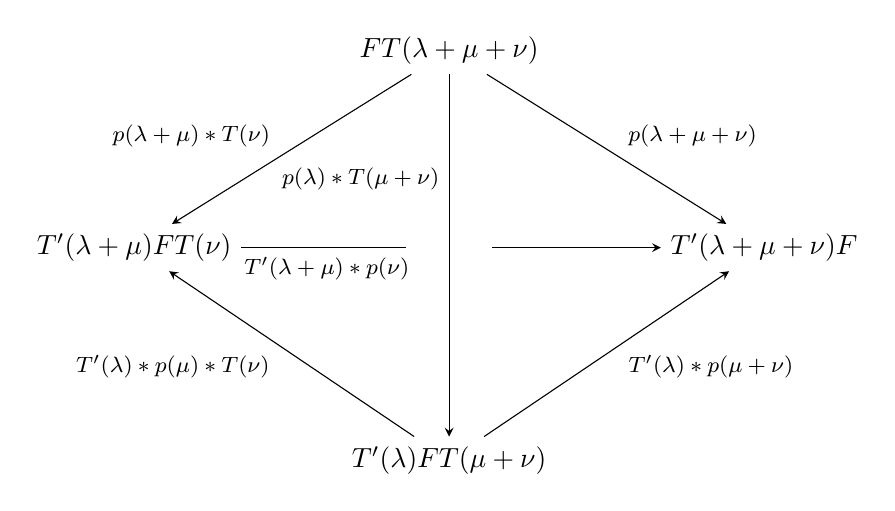
\begin{tikzpicture}[x=1cm,y=1cm,>=stealth]
    \node (a) at (0,3.2) {$FT(\lambda+\mu+\nu)$};
    \node (b) at (-4,0.7) {$T'(\lambda+\mu)FT(\nu)$};
    \node (c) at (4,0.7) {$T'(\lambda+\mu+\nu)F$};
    \node (d) at (0,-2.0) {$T'(\lambda)FT(\mu+\nu)$};
    \draw[->] (a) -- node[above left,pos=.55,font=\footnotesize]
      {$p(\lambda+\mu)*T(\nu)$} (b);
    \draw[->] (a) -- node[above right,pos=.55,font=\footnotesize]
      {$p(\lambda+\mu+\nu)$} (c);
    \draw[->] (a) -- node[left,pos=.29,font=\footnotesize]
      {$p(\lambda)*T(\mu+\nu)$} (d);
    \coordinate (bc-left) at (-0.55,0.7);
    \coordinate (bc-right) at (0.55,0.7);
    \draw (b) -- node[below,pos=.52,font=\footnotesize]
      {$T'(\lambda+\mu)*p(\nu)$} (bc-left);
    \draw[->] (bc-right) -- (c);
    \draw[->] (d) -- node[below left,pos=.55,font=\footnotesize]
      {$T'(\lambda)*p(\mu)*T(\nu)$} (b);
    \draw[->] (d) -- node[below right,pos=.55,font=\footnotesize]
      {$T'(\lambda)*p(\mu+\nu)$} (c);
  \end{tikzpicture}
\end{center}

\VerdierSemanticAnchor{ch1-1-5-5-faces}
此图呈四面体形，其四个面分别为图
$D(\lambda,\mu+\nu)$、$D(\lambda+\mu,\nu)$、
$D(\lambda,\mu)T(\nu)$ 与 $T'(\lambda)D(\mu,\nu)$。
于是考察四种可能情形并使用余循环关系，即可证明 (1.5.4.5)。

\VerdierSemanticAnchor{ch1-1-5-5-reduction}
在一般情形中，需要引入的图稍复杂一些；但利用恒等式 (1.2.1.3)，
论证可归结为上面所概述的论证。要得到 (1.5.3.5) 的证明，只需在同一图中置
\[
  \lambda=qe_1,\qquad \mu=q'e_1,\qquad \nu=q''e_1.
\]

\VerdierSourcePageBlock{0056}%
\VerdierSemanticAnchor{ch1-1-5-6}
\noindent\textbf{图 1.5.6.}\quad
现在证明断言 (1.5.4.3)。证明基于下图；为简便起见，我们仍把它写在
过渡同构 $c,c'$ 都是恒等态射的情形：

\VerdierSemanticAnchor{ch1-1-5-7}
\noindent\textbf{1.5.7.}

\VerdierSemanticAnchor{ch1-1-5-7-diagram}
\begin{center}
  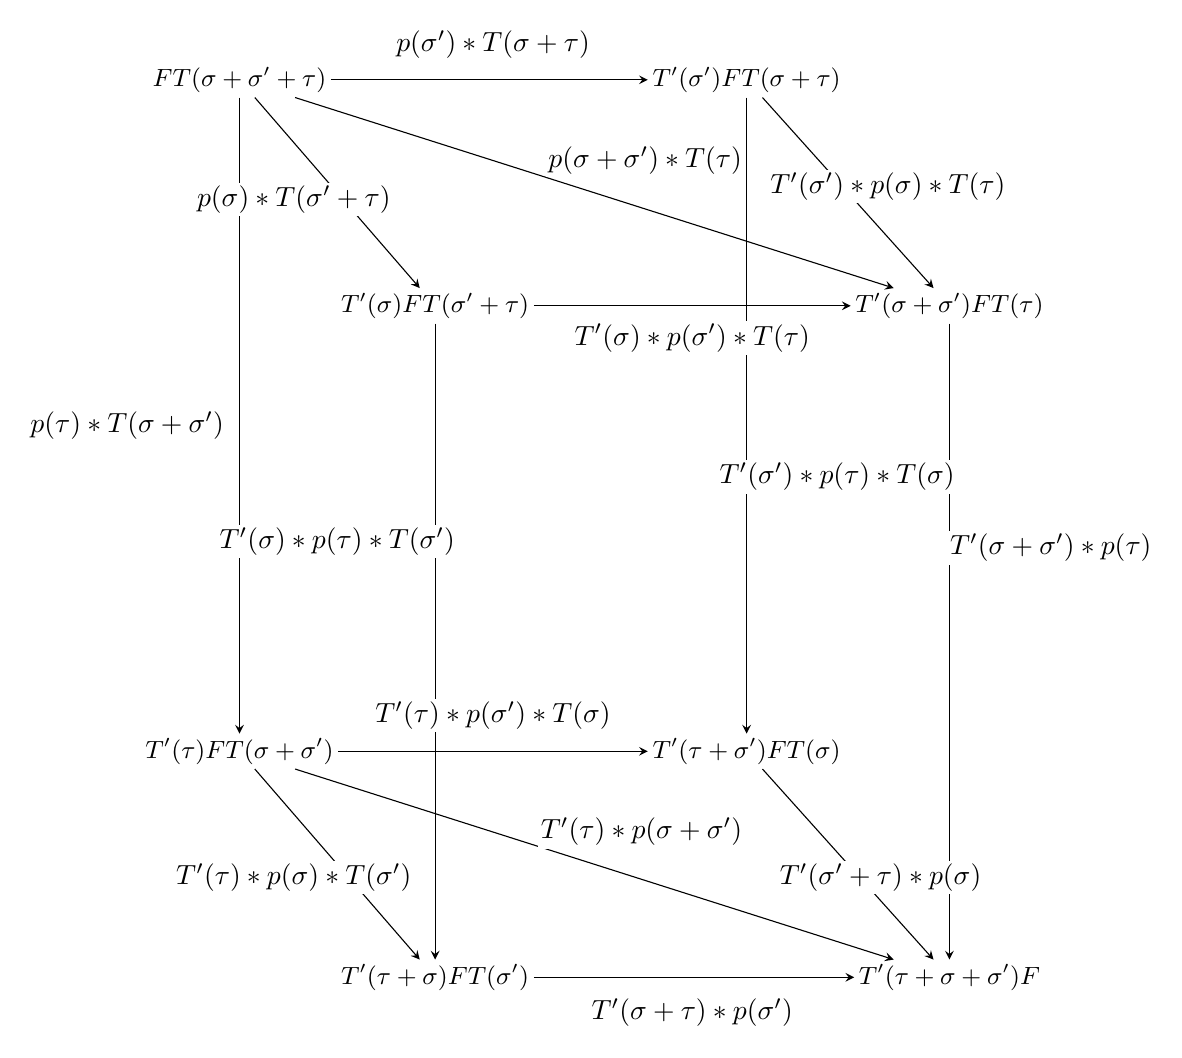
\begin{tikzpicture}[x=.92cm,y=.82cm,>=stealth,
      object/.style={inner sep=1.5pt,font=\small},
      lab/.style={font=\normalsize,fill=white,inner sep=1pt}]
    \node[object] (a) at (-5.8,13.0) {$FT(\sigma+\sigma'+\tau)$};
    \node[object] (b) at (1.2,13.0) {$T'(\sigma')FT(\sigma+\tau)$};
    \node[object] (c) at (-3.1,9.5) {$T'(\sigma)FT(\sigma'+\tau)$};
    \node[object] (d) at (4.0,9.5) {$T'(\sigma+\sigma')FT(\tau)$};
    \node[object] (e) at (-5.8,2.6) {$T'(\tau)FT(\sigma+\sigma')$};
    \node[object] (f) at (1.2,2.6) {$T'(\tau+\sigma')FT(\sigma)$};
    \node[object] (g) at (-3.1,-0.9) {$T'(\tau+\sigma)FT(\sigma')$};
    \node[object] (h) at (4.0,-0.9) {$T'(\tau+\sigma+\sigma')F$};

    \draw[->] (a) -- (b);
    \draw[->] (a) -- (c);
    \draw[->] (a) -- (d);
    \draw[->] (a) -- (e);
    \draw[->] (b) -- (d);
    \draw[->] (b) -- (f);
    \draw[->] (c) -- (d);
    \draw[->] (c) -- (g);
    \draw[->] (d) -- (h);
    \draw[->] (e) -- (f);
    \draw[->] (e) -- (g);
    \draw[->] (e) -- (h);
    \draw[->] (f) -- (h);
    \draw[->] (g) -- (h);

    \node[lab] at (-2.3,13.55) {$p(\sigma')*T(\sigma+\tau)$};
    \node[lab] at (-5.05,11.15) {$p(\sigma)*T(\sigma'+\tau)$};
    \node[lab] at (-0.2,11.75) {$p(\sigma+\sigma')*T(\tau)$};
    \node[lab] at (-7.35,7.65) {$p(\tau)*T(\sigma+\sigma')$};
    \node[lab] at (3.15,11.35) {$T'(\sigma')*p(\sigma)*T(\tau)$};
    \node[lab] at (2.45,6.85) {$T'(\sigma')*p(\tau)*T(\sigma)$};
    \node[lab] at (0.45,9.00) {$T'(\sigma)*p(\sigma')*T(\tau)$};
    \node[lab] at (-4.45,5.85) {$T'(\sigma)*p(\tau)*T(\sigma')$};
    \node[lab] at (5.40,5.75) {$T'(\sigma+\sigma')*p(\tau)$};
    \node[lab] at (-2.3,3.15) {$T'(\tau)*p(\sigma')*T(\sigma)$};
    \node[lab] at (-5.05,0.65) {$T'(\tau)*p(\sigma)*T(\sigma')$};
    \node[lab] at (-0.25,1.35) {$T'(\tau)*p(\sigma+\sigma')$};
    \node[lab] at (3.05,0.65) {$T'(\sigma'+\tau)*p(\sigma)$};
    \node[lab] at (0.45,-1.45) {$T'(\sigma+\tau)*p(\sigma')$};
  \end{tikzpicture}
\end{center}

\VerdierSemanticAnchor{ch1-1-5-7-delta-intro}
以 $\Delta(\sigma,\tau)$ 表示图
$\textup{(1.5.4.2)}_{\sigma,\tau}$。上图%
\VerdierSourcePageContinue{0057}%
\VerdierSemanticAnchor{ch1-1-5-7-continuation}
显现出五个竖直图，依次为：

\VerdierSemanticAnchor{ch1-1-5-7-vertical}
\[
  T'(\sigma')\Delta(\sigma,\tau),\quad
  T'(\sigma)\Delta(\sigma',\tau),\quad
  \Delta(\sigma,\tau)T(\sigma'),\quad
  \Delta(\sigma',\tau)T(\sigma),\quad
  \Delta(\sigma+\sigma',\tau).
\]

同样，它还显现出四个水平图，依次为：

\VerdierSemanticAnchor{ch1-1-5-7-horizontal}
\[
  D(\sigma,\sigma')T(\tau),\quad
  D(\sigma',\sigma)T(\tau),\quad
  T'(\tau)D(\sigma,\sigma'),\quad
  T'(\tau)D(\sigma',\sigma).
\]

\VerdierSemanticAnchor{ch1-1-5-7-conclusion}
由归纳假设，图 $D(\sigma,\sigma')$ 与 $D(\sigma',\sigma)$ 分别为
$\alpha(\sigma,\sigma')$-交换和 $\alpha(\sigma',\sigma)$-交换的。
考察三种可能情形，便得到断言 (1.5.4.3) 的第一部分。交换 $\sigma$ 与
$\tau$ 的角色即可得到其第二部分。在一般情形中，需要引入的图更复杂；
但利用恒等式 (1.2.1.3)，论证可归结为上面给出的论证。

\VerdierSemanticAnchor{ch1-1-5-8}
\noindent\textbf{注 1.5.8.}\quad
命题 (1.5.2) 特别适用于余循环 $\alpha$ 平凡的情形。这时可以验证，
即使范畴 $\mathcal C'$ 不再必为加法范畴，该命题及其证明仍可逐字照搬。

\VerdierSemanticAnchor{ch1-1-5-9}
\noindent\textbf{1.5.9.}\quad
设

\VerdierSemanticAnchor{ch1-1-5-9-functors}
\[
  (F_1,p_1),(F_2,p_2)\colon
  (\mathcal C,\mathbb Z^n,T,c)
  \longrightarrow
  (\mathcal C',\mathbb Z^n,T',c')
\]
为分别由两个正规化余循环
$\alpha_1,\alpha_2\in Z^2(\mathbb Z^n,\mathbb Z/2\mathbb Z)$
扭曲的两个 $\mathbb Z^n$-函子，并设
$\beta\colon\mathbb Z^n\to\mathbb Z/2\mathbb Z$ 为满足

\VerdierSemanticAnchor{ch1-1-5-9-eq1}
\begin{equation}
  \alpha_2(\sigma_1,\sigma_2)\alpha_1^{-1}(\sigma_1,\sigma_2)
  =\beta(\sigma_2)\beta(\sigma_1\sigma_2)^{-1}\beta(\sigma_1),
  \qquad \sigma_1,\sigma_2\in\mathbb Z^n,
  \tag{1.5.9.1}
\end{equation}
的映射，又设 $u\colon(F_1,p_1)\to(F_2,p_2)$ 为函子的一个
$\beta$-态射 (1.4.6)。令 $e_1,\ldots,e_n$ 为 $\mathbb Z^n$ 的典范基。
对每个 $i\in[1,n]$，下图为 $\beta(e_i)$-交换的：

\VerdierSemanticAnchor{ch1-1-5-9-eq2}
\begin{equation}
  \mbox{%
    $\begin{tikzcd}[ampersand replacement=\&,column sep=6em,row sep=4em]
      F_1T(e_i)
        \arrow[r,"{p_1(e_i)}"]
        \arrow[d,"{u*T(e_i)}"']
        \& T'(e_i)F_1
          \arrow[d,"{T'(e_i)*u}"] \\
      F_2T(e_i)
        \arrow[r,"{p_2(e_i)}"]
        \& T'(e_i)F_2
    \end{tikzcd}$%
  }\;.
  \tag{1.5.9.2}
\end{equation}

\VerdierSourcePageBlock{0058}%
\VerdierSemanticAnchor{ch1-1-5-10-converse}
\noindent\textbf{反过来：}\par

\VerdierSemanticAnchor{ch1-1-5-10}
\VerdierSemanticAnchor{ch1-1-5-10-proposition}
\noindent\textbf{命题 1.5.10.}\quad
\emph{设 $u\colon F_1\to F_2$ 为底层函子之间的一个态射；若对每个
$i\in[1,n]$，图 (1.5.9.2) 都为 $\beta(e_i)$-交换的，
则 $u$ 是函子的一个 $\beta$-态射。}

\VerdierSemanticAnchor{ch1-1-5-10-proof}
事实上，对每个 $\sigma\in\mathbb Z^n$，以 $R(\sigma)$ 表示性质：

\VerdierSemanticAnchor{ch1-1-5-10-property}
\noindent\emph{$(R(\sigma))$\qquad 下图为 $\beta(\sigma)$-交换的：}

\VerdierSemanticAnchor{ch1-1-5-10-eq1}
\begin{equation}
  \mbox{%
    $\begin{tikzcd}[ampersand replacement=\&,column sep=6em,row sep=4em]
      F_1T(\sigma)
        \arrow[r,"{p_1(\sigma)}"]
        \arrow[d,"{u*T(\sigma)}"']
        \& T'(\sigma)F_1
          \arrow[d,"{T'(\sigma)*u}"] \\
      F_2T(\sigma)
        \arrow[r,"{p_2(\sigma)}"]
        \& T'(\sigma)F_2
    \end{tikzcd}$%
  }\;.
  \tag*{\ensuremath{(1.5.10.1)_{\sigma}}}
\end{equation}

考察各图 $(1.5.10.1)_{\sigma_1}$、$(1.5.10.1)_{\sigma_2}$ 与
$(1.5.10.1)_{\sigma_1+\sigma_2}$，立即得到：

\VerdierSemanticAnchor{ch1-1-5-10-closure}
\noindent\emph{若性质 $R(\sigma_1)$、$R(\sigma_2)$、
$R(\sigma_1+\sigma_2)$ 中有两个成立，则第三个也成立。}

\VerdierSemanticAnchor{ch1-1-5-10-conclusion}
此外，由假设，性质 $R(e_i)$（$i\in[1,n]$）与 $R(0)$ 均成立。
由此立即可知，$R(\sigma)$ 对每个 $\sigma\in\mathbb Z^n$ 都成立。

\VerdierSemanticAnchor{ch1-1-5-11}
\noindent\textbf{1.5.11.}\quad
一个严格 $\mathbb Z^n$-范畴，是一个装备了 $\mathbb Z^n$ 到其自同构群
的表示的范畴。要定义这样的表示，当然只需给出 $n$ 个两两交换的自同构
$T(e_1),\ldots,T(e_n)$。

\VerdierSemanticAnchor{ch1-1-5-12}
\noindent\textbf{1.5.12.}\quad
在一个给定范畴上确定（不必严格的）$\mathbb Z^n$-范畴结构，问题要复杂得多。
例如，只考虑范畴 $\mathcal C$ 上满足每个 $\sigma\in\mathbb Z^n$ 都有
$T(\sigma)=\text{$\mathcal C$ 上的恒等函子}$ 的 $\mathbb Z^n$-范畴结构。
这时必须对每一对 $\sigma_1,\sigma_2\in\mathbb Z^n$，给出
$\mathcal C$ 的恒等函子的自同构群中的一个元素
$c(\sigma_1,\sigma_2)$（该群为交换群），并要求这些数据满足恒等式
(1.2.1.3)。因此，要给出这样的结构，就必须给出一个取值于
$\mathcal C$ 的恒等函子自同构群的、$\mathbb Z^n$ 上的正规化非齐次
2-余循环。还可立即验证：两个这样的结构可由一个满足
$F=\text{$\mathcal C$ 上的恒等函子}$ 的 $\mathbb Z^n$-函子 $(F,m)$
同构，当且仅当相应余循环属于同一上同调类。

\VerdierSourcePageBlock{0059}%
\VerdierSemanticAnchor{ch1-1-5-13}
\noindent\textbf{1.5.13.}\quad
本书将使用的 $\mathbb Z^n$-范畴都是严格范畴。因此，我们不打算在一般情形下
讨论 (1.5.12) 所指出的问题。不过，(1.5.12) 的例子表明，在一个范畴
$\mathcal C$ 上确定 $\mathbb Z$-范畴结构格外简单。事实确实如此。
以 $E\text{-}\operatorname{Cat}$ 表示如下 $U$-范畴：其对象是属于 $U$
且装备了一个等价

\VerdierSemanticAnchor{ch1-1-5-13-eq1}
\begin{equation}
  T\colon\mathcal C\longrightarrow\mathcal C
  \tag{1.5.13.1}
\end{equation}
的范畴；其态射是装备了同构

\VerdierSemanticAnchor{ch1-1-5-13-eq2}
\begin{equation}
  m\colon FT\longrightarrow T'F
  \tag{1.5.13.2}
\end{equation}
的函子 $F\colon\mathcal C\to\mathcal C'$。

于是显然有从 $U$-范畴 $\mathbb Z\text{-}\operatorname{Cat}$ 到
$U$-范畴 $E\text{-}\operatorname{Cat}$ 的函子

\VerdierSemanticAnchor{ch1-1-5-13-eq3}
\begin{equation}
  R\colon \mathbb Z\text{-}\operatorname{Cat}
  \longrightarrow E\text{-}\operatorname{Cat}.
  \tag{1.5.13.3}
\end{equation}

\VerdierSemanticAnchor{ch1-1-5-13-action}
函子 $R$ 把 $\mathbb Z$-范畴 $(\mathcal C,\mathbb Z,T,c)$ 映到装备了等价
$T(1)\colon\mathcal C\to\mathcal C$ 的范畴 $\mathcal C$，并把每个
$\mathbb Z$-函子
\[
  (F,m)\colon(\mathcal C,\mathbb Z,T,c)
  \longrightarrow(\mathcal C',\mathbb Z,T',c')
\]
映到装备了同构 $m(1)\colon FT(1)\to T'(1)F$ 的函子 $F$。

\VerdierSemanticAnchor{ch1-1-5-14}
\VerdierSemanticAnchor{ch1-1-5-14-proposition}
\noindent\textbf{命题 1.5.14.}\quad
\emph{函子 $R$ 是范畴的等价。}

\VerdierSemanticAnchor{ch1-1-5-14-proof}
我们只给出证明的若干说明。命题 (1.5.2) 与注 (1.5.8) 表明 $R$ 充分忠实，
因此只需证明 $R$ 本质满。设
$(\mathcal C,T\colon\mathcal C\to\mathcal C)$ 为装备了一个等价的范畴。
取 $T$ 的一个拟逆函子 $T^{-1}\colon\mathcal C\to\mathcal C$，并令

\VerdierSemanticAnchor{ch1-1-5-14-eq1}
\begin{equation}
  \begin{aligned}
    u&\colon\operatorname{id}_{\mathcal C}\longrightarrow TT^{-1},\\
    v&\colon\operatorname{id}_{\mathcal C}\longrightarrow T^{-1}T
  \end{aligned}
  \tag{1.5.14.1}
\end{equation}
为伴随同构。

对每个整数 $n>0$，函子 $T^n$ 与 $(T^{-1})^n$ 互为伴随，因而有伴随同构

\VerdierSemanticAnchor{ch1-1-5-14-eq2}
\begin{equation}
  \begin{aligned}
    u^{(n)}&\colon\operatorname{id}_{\mathcal C}
      \longrightarrow T^n(T^{-1})^n,\\
    v^{(n)}&\colon\operatorname{id}_{\mathcal C}
      \longrightarrow (T^{-1})^nT^n.
  \end{aligned}
  \tag{1.5.14.2}
\end{equation}%
\VerdierSourcePageContinue{0060}%
\VerdierSemanticAnchor{ch1-1-5-14-continuation}
然后令：

\VerdierSemanticAnchor{ch1-1-5-14-eq3}
\begin{equation}
  \begin{aligned}
    T(0)&=\operatorname{id}_{\mathcal C},\\
    T(n)&=T^n, && n>0,\\
    T(n)&=(T^{-1})^{-n}, && n<0.
  \end{aligned}
  \tag{1.5.14.3}
\end{equation}

\VerdierSemanticAnchor{ch1-1-5-14-cocycle-data}
再对每一对整数 $(n,n')$，如下定义同构
\[
  c(n',n)\colon T(n+n')\longrightarrow T(n)T(n')
\]
：

\VerdierSemanticAnchor{ch1-1-5-14-eq4}
\begin{equation}
  \begin{aligned}
    n,n'&\geq 0,
      &c(n',n)&=\operatorname{id},\\
    n,n'&\leq 0,
      &c(n',n)&=\operatorname{id},\\
    n'&\leq 0, n\geq 0, n+n'\leq 0,
      &c(n',n)&=u^{(n)}\mathbin{*}T(n+n'),\\
    n'&\leq 0, n\geq 0, n+n'\geq 0,
      &c(n',n)&=T(n+n')\mathbin{*}u^{(-n')},\\
    n'&\geq 0, n\leq 0, n+n'\leq 0,
      &c(n',n)&=T(n+n')\mathbin{*}v^{(n')},\\
    n'&\geq 0, n\leq 0, n+n'\geq 0,
      &c(n',n)&=v^{(-n)}\mathbin{*}T(n+n').
  \end{aligned}
  \tag{1.5.14.4}
\end{equation}

\VerdierSemanticAnchor{ch1-1-5-14-conclusion}
为了确认这样确实定义了一个 $\mathbb Z$-范畴，还需验证 (1.2.1.3) 型的
恒等式成立。该验证建立在态射 $u^{(n)}$ 与 $v^{(n)}$ 所满足的经典恒等式上。
我们把细节留给读者。

\VerdierSemanticAnchor{ch1-1-6}
\subsection{Koszul 余循环与符号规则}

\VerdierSemanticAnchor{ch1-1-6-1}
\noindent\textbf{1.6.1.}\quad
设 $e_1,\ldots,e_n$ 为 $\mathbb Z^n$ 的一组基。对
$i,j\in[1,n]$ 且 $i\neq j$，以 $\mathbb Z^n_{i,j}$ 表示由 $e_i$ 与
$e_j$ 生成的 $\mathbb Z^n$ 的子群。限制同态给出同态

\VerdierSemanticAnchor{ch1-1-6-1-eq1}
\begin{equation}
  H^2(\mathbb Z^n,\mathbb Z/2\mathbb Z)
  \longrightarrow
  \bigoplus_{\substack{i,j\in[1,n]\\ i<j}}
    H^2(\mathbb Z^n_{i,j},\mathbb Z/2\mathbb Z).
  \tag{1.6.1.1}
\end{equation}

我们有（典范）同构

\VerdierSemanticAnchor{ch1-1-6-1-eq2}
\begin{equation}
  H^2(\mathbb Z^n_{i,j},\mathbb Z/2\mathbb Z)
  \simeq \mathbb Z/2\mathbb Z.
  \tag{1.6.1.2}
\end{equation}

\VerdierSemanticAnchor{ch1-1-6-1-conclusion}
同态 (1.6.1.1) 是同构。

\VerdierSourcePageBlock{0061}%
\VerdierSemanticAnchor{ch1-1-6-2}
\VerdierSemanticAnchor{ch1-1-6-2-proposition}
\noindent\textbf{命题 1.6.2.}\quad

\VerdierSemanticAnchor{ch1-1-6-2-part1}
\noindent\emph{1) 设
$\alpha\in Z^2(\mathbb Z^n,\mathbb Z/2\mathbb Z)$ 为正规化非齐次余循环，
$\dot\alpha\in H^2(\mathbb Z^n,\mathbb Z/2\mathbb Z)$ 为其上同调类，
$\dot\alpha_{i,j}\in H^2(\mathbb Z^n_{i,j},\mathbb Z/2\mathbb Z)$ 为其
各分量。则（利用 (1.6.1.2)）：}

\VerdierSemanticAnchor{ch1-1-6-2-eq1}
\begin{equation}
  \dot\alpha_{i,j}
  =\alpha(e_i,e_j)^{-1}\alpha(e_j,e_i).
  \tag{1.6.2.1}
\end{equation}

\VerdierSemanticAnchor{ch1-1-6-2-convention}
\noindent\emph{（$\mathbb Z/2\mathbb Z$ 的群运算采用乘法记号。）}

\VerdierSemanticAnchor{ch1-1-6-2-part2}
\noindent\emph{2) 设 $\alpha_1$ 与 $\alpha_2$ 是
$Z^2(\mathbb Z^n,\mathbb Z/2\mathbb Z)$ 中两个上同调等价的元素，并对每个
$i\in[1,n]$ 给定元素 $\beta_i\in\mathbb Z/2\mathbb Z$。则存在唯一映射}

\VerdierSemanticAnchor{ch1-1-6-2-beta-map}
\begin{equation*}
  \beta\colon\mathbb Z^n\longrightarrow\mathbb Z/2\mathbb Z
\end{equation*}
\noindent\emph{满足：}

\VerdierSemanticAnchor{ch1-1-6-2-eq2}
\begin{equation}
  \begin{aligned}
    \alpha_2(\sigma_1,\sigma_2)\alpha_1^{-1}(\sigma_1,\sigma_2)
      &=\beta(\sigma_2)\beta(\sigma_1+\sigma_2)^{-1}\beta(\sigma_1),\\[-1mm]
    &\hspace{7em}\text{其中 }\sigma_1,\sigma_2\in\mathbb Z^n,
  \end{aligned}
  \tag{1.6.2.2}
\end{equation}

\VerdierSemanticAnchor{ch1-1-6-2-eq3}
\begin{equation}
  \beta(e_i)=\beta_i.
  \tag{1.6.2.3}
\end{equation}

\VerdierSemanticAnchor{ch1-1-6-2-proof}
\VerdierSemanticAnchor{ch1-1-6-2-proof-first}
为证明第一个断言，我们归约到 $n=2$ 的情形，并直接验证当 $\alpha$ 加上一个
余边界时，量 $\alpha(e_i,e_j)^{-1}\alpha(e_j,e_i)$ 不变。当 $\alpha$ 是
余边界时，它是对称的，因此公式 (1.6.2.1) 在此情形成立。另一方面，余循环

\VerdierSemanticAnchor{ch1-1-6-2-alpha0}
\begin{equation*}
  \alpha_0(p_1e_i+q_1e_j,p_2e_i+q_2e_j)=(-1)^{q_1p_2}
\end{equation*}
不与 $0$ 上同调等价，因为

\VerdierSemanticAnchor{ch1-1-6-2-alpha0-test}
\begin{equation*}
  \alpha_0(e_i,e_j)^{-1}\alpha_0(e_j,e_i)=-1,
\end{equation*}
并且每个不与零上同调等价的余循环都与 $\alpha_0$ 上同调等价。

\VerdierSemanticAnchor{ch1-1-6-2-proof-second}
为证明第二个断言，注意 (1.6.2.2) 的任意两个解之差是一个群同态。因此总能
唯一地用一个群同态修正 (1.6.2.2) 的一个解，使它在各 $e_i$ 上取预先指定的值。

\VerdierSemanticAnchor{ch1-1-6-3}
\VerdierSemanticAnchor{ch1-1-6-3-definition}
\noindent\textbf{定义 1.6.3.}\quad
设 $e_1,\ldots,e_n$ 为 $\mathbb Z^n$ 的一组基。\emph{相对于基
$e_1,\ldots,e_n$ 的 Koszul 类}，是
$H^2(\mathbb Z^n,\mathbb Z/2\mathbb Z)$ 中唯一一个在各群
$H^2(\mathbb Z^n_{i,j},\mathbb Z/2\mathbb Z)$ 上的限制均非零的元素。

\VerdierSemanticAnchor{ch1-1-6-3-basis-dependence}
注意，Koszul 类的定义涉及 $\mathbb Z^n$ 的一组基的选择。一般而言，与两组
不同基相联系的 Koszul 类也不同。

\VerdierSemanticAnchor{ch1-1-6-3-filtration}
设 $e_1,\ldots,e_n$ 为一组按照 $[1,n]$ 上自然次序排列的基。以
$\mathbb Z^n(\leq i)$（分别以 $\mathbb Z^n(\geq i)$）表示由满足
$j\leq i$（分别满足 $j\geq i$）的 $e_j$ 生成的 $\mathbb Z^n$ 的子群。

\VerdierSourcePageBlock{0062}%
\VerdierSemanticAnchor{ch1-1-6-4}
\VerdierSemanticAnchor{ch1-1-6-4-definition}
\noindent\textbf{定义 1.6.4.}\quad
\emph{相对于 $\mathbb Z^n$ 的一组有序基 $e_1,\ldots,e_n$ 的 Koszul
余循环}，是相对于基 $e_1,\ldots,e_n$ 的 Koszul 类中满足下式的唯一余循环
$\alpha$：

\VerdierSemanticAnchor{ch1-1-6-4-eq1}
\begin{equation}
  \alpha(\sigma_1,\sigma_2)=1
  \quad
  \forall\sigma_1\in\mathbb Z^n(\leq i),\quad
  \forall\sigma_2\in\mathbb Z^n(\geq i),\quad
  \forall i\in[1,n].
  \tag{1.6.4.1}
\end{equation}

\VerdierSemanticAnchor{ch1-1-6-4-coordinate-intro}
设
$\sigma_1=\sum_{i=1}^{n}p_i e_i$ 与
$\sigma_2=\sum_{i=1}^{n}q_i e_i$
为 $\mathbb Z^n$ 的两个元素，则：

\VerdierSemanticAnchor{ch1-1-6-4-eq2}
\begin{equation}
  \alpha(\sigma_1,\sigma_2)
  =(-1)^{\left(\sum_{i<j}q_i p_j\right)}.
  \tag{1.6.4.2}
\end{equation}

\VerdierSemanticAnchor{ch1-1-6-4-justification}
这个定义需要说明。满足 (1.6.4.1) 的 Koszul 类中的余循环显然存在：直接计算
可知余循环 (1.6.4.2) 满足 (1.6.4.1)，并且属于 Koszul 类 (1.6.2)。为验证
唯一性，只需注意每个与余循环 $\alpha$ 上同调等价的余循环都形如

\VerdierSemanticAnchor{ch1-1-6-4-cohomologous-form}
\begin{equation*}
  \alpha_1(\sigma_1,\sigma_2)
  =\alpha(\sigma_1,\sigma_2)
   \beta(\sigma_2)\beta(\sigma_1+\sigma_2)^{-1}\beta(\sigma_1)
\end{equation*}
并且这样的余循环具有性质 (1.6.4.1)，当且仅当

\VerdierSemanticAnchor{ch1-1-6-4-condition}
\begin{equation*}
  \beta(\sigma_1+\sigma_2)=\beta(\sigma_1)\beta(\sigma_2)
  \quad
  \forall i,\quad
  \forall\sigma_1\in\mathbb Z^n(\leq i),\quad
  \forall\sigma_2\in\mathbb Z^n(\geq i).
\end{equation*}

\VerdierSemanticAnchor{ch1-1-6-4-uniqueness}
由此立即得到 $\beta\colon\mathbb Z^n\to\mathbb Z/2\mathbb Z$ 是群同态，
因而 $\alpha_1=\alpha$。

\VerdierSemanticAnchor{ch1-1-6-5}
\VerdierSemanticAnchor{ch1-1-6-5-order-dependence}
\noindent\textbf{1.6.5.}\quad
Koszul 余循环的定义本质上依赖于赋予 $\mathbb Z^n$ 的基
$e_1,\ldots,e_n$ 的全序。以 $\leq$ 表示 $[1,n]$ 上的自然次序，以
$\leq_s$ 表示 $[1,n]$ 上的一个全序。设 $s$ 为 $[1,n]$ 上唯一满足下式的置换：

\VerdierSemanticAnchor{ch1-1-6-5-eq1}
\begin{equation}
  i\leq_s j\quad\Longleftrightarrow\quad s(i)\leq s(j).
  \tag{1.6.5.1}
\end{equation}

\VerdierSemanticAnchor{ch1-1-6-5-cocycles}
设 $\alpha$ 与 $\alpha_s$ 分别为相对于次序 $\leq$ 与 $\leq_s$ 的 Koszul
余循环。则：

\VerdierSemanticAnchor{ch1-1-6-5-eq2}
\VerdierSemanticAnchor{ch1-1-6-5-eq2-natural}
\VerdierSemanticAnchor{ch1-1-6-5-eq2-coordinates}
\VerdierSemanticAnchor{ch1-1-6-5-eq2-permuted}
\begin{equation}
  \begin{aligned}
    \alpha(\sigma_1,\sigma_2)
      &=(-1)^{\left(\sum_{i<j}q_i p_j\right)},\\
    \sigma_1&=\sum_i p_i e_i,
      \qquad \sigma_2=\sum_i q_i e_i,\\
    \alpha_s(\sigma_1,\sigma_2)
      &=(-1)^{\left(\sum_{s(i)<s(j)}q_i p_j\right)},
  \end{aligned}
  \tag{1.6.5.2}
\end{equation}
\VerdierSemanticAnchor{ch1-1-6-5-open}%
\VerdierSourcePageContinue{0063}%
\VerdierSemanticAnchor{ch1-1-6-5-continuation}
由此立即得到：

\VerdierSemanticAnchor{ch1-1-6-5-deduction}
\VerdierSemanticAnchor{ch1-1-6-5-beta-s-coboundary}
\begin{equation*}
  \alpha_s(\sigma_1,\sigma_2)\alpha(\sigma_1,\sigma_2)^{-1}
  =\beta_s(\sigma_2)\beta_s(\sigma_1+\sigma_2)^{-1}\beta_s(\sigma_1),
\end{equation*}

\VerdierSemanticAnchor{ch1-1-6-5-eq3}
\VerdierSemanticAnchor{ch1-1-6-5-eq3-beta}
\VerdierSemanticAnchor{ch1-1-6-5-eq3-basis}
\begin{equation}
  \begin{aligned}
    \beta_s(\sigma_1)
      &=(-1)^{\left(
          \sum_{\substack{i<j\\s(i)>s(j)}}p_i p_j
        \right)},\\
    \beta_s(e_i)&=1,
      \qquad \forall i\in[1,n].
  \end{aligned}
  \tag{1.6.5.3}
\end{equation}

\VerdierSemanticAnchor{ch1-1-6-5-application}
因此，由 (1.6.2)，每个满足下式的映射
$\beta\colon\mathbb Z^n\to\mathbb Z/2\mathbb Z$

\VerdierSemanticAnchor{ch1-1-6-5-eq4}
\begin{equation}
  \alpha_s(\sigma_1,\sigma_2)\alpha(\sigma_1,\sigma_2)^{-1}
  =\beta(\sigma_2)\beta(\sigma_1+\sigma_2)^{-1}\beta(\sigma_1)
  \tag{1.6.5.4}
\end{equation}

\VerdierSemanticAnchor{ch1-1-6-5-eq5-intro}
都形如

\VerdierSemanticAnchor{ch1-1-6-5-eq5}
\begin{equation}
  \beta=\beta_s\eta,
  \tag{1.6.5.5}
\end{equation}

\VerdierSemanticAnchor{ch1-1-6-5-closure}
其中 $\eta\colon\mathbb Z^n\to\mathbb Z/2\mathbb Z$ 是唯一一个在
$e_j\in\mathbb Z^n$ 上取值为 $\beta(e_j)$ 的群同态。

\VerdierSemanticAnchor{ch1-1-6-6}
\VerdierSemanticAnchor{ch1-1-6-6-product-setup}
\noindent\textbf{1.6.6.}\quad
设 $(C_i,\mathbb Z,T_i,c_i)$，$1\leq i\leq n$，为 $\mathbb Z$-范畴，
并设 $(D,\mathbb Z,T,c)$ 为加法 $\mathbb Z$-范畴。以
$(C,\mathbb Z^n,T,c)$ 表示各 $(C_i,\mathbb Z,T_i,c_i)$ 的乘积范畴。
群 $\mathbb Z^n$ 自然装备了有序基 $e_1,\ldots,e_n$。它依下式在同构意义下
作用于 $C$（这里采用 (1.3.12) 引入的右侧记号）：

\VerdierSemanticAnchor{ch1-1-6-6-eq1}
\begin{equation}
  (X_1,\ldots,X_n)[\sigma]
  =(X_1[l_1],\ldots,X_n[l_n]),
  \qquad
  \sigma=\sum_{i=1}^{n}l_i e_i.
  \tag{1.6.6.1}
\end{equation}

\VerdierSemanticAnchor{ch1-1-6-6-phi-action}
设 $\varphi\colon\mathbb Z^n\to\mathbb Z$ 为同态
$\varphi(\sum_{i=1}^{n}l_i e_i)=\sum_{i=1}^{n}l_i$。
让 $\mathbb Z^n$ 通过 $\varphi$ 作用于 $D$（1.4.1）。在此情形中，我们总采用
以下约定：

\VerdierSemanticAnchor{ch1-1-6-6-sign-rule-1}
\noindent\textbf{符号规则 I：}
\emph{除非另有明确说明，从 $C$ 到 $D$ 的函子总是相对于有序基
$e_1,\ldots,e_n$ 的 Koszul 余循环所扭曲的 $\mathbb Z^n$-函子。}

\VerdierSemanticAnchor{ch1-1-6-6-sign-rule-2}
\noindent\textbf{符号规则 II：}
\emph{除非另有明确说明，函子的态射总是相对于平凡同态
$\beta\colon\mathbb Z^n\to\mathbb Z/2\mathbb Z$ 的 $\mathbb Z^n$-函子态射
（1.4.6）。}

\VerdierSourcePageBlock{0064}%
\VerdierSemanticAnchor{ch1-1-6-6-functor-characterization}
由命题 (1.5.2)，给定一个从 $C$ 到 $D$ 的函子，等价于给定一个函子

\VerdierSemanticAnchor{ch1-1-6-6-eq2}
\begin{equation}
  (X_1,\ldots,X_n)\longmapsto F(X_1,\ldots,X_n)
  \tag{1.6.6.2}
\end{equation}

\VerdierSemanticAnchor{ch1-1-6-6-transition-isomorphisms}
以及函子同构

\VerdierSemanticAnchor{ch1-1-6-6-eq3}
\begin{equation}
  p_i\colon
  F(X_1,\ldots,X_i[1],\ldots,X_n)
  \xrightarrow{\ \sim\ }
  F(X_1,\ldots,X_n)[1]
  \tag{1.6.6.3}
\end{equation}

\VerdierSemanticAnchor{ch1-1-6-6-anticommutativity}
并要求图 (1.5.1.2)

\VerdierSemanticAnchor{ch1-1-6-6-anticommutativity-diagram}
\begin{equation*}
  \mbox{%
    $\begin{tikzcd}[ampersand replacement=\&,column sep=2.8em,row sep=3.8em]
      F(X_1,\ldots,X_i[1],\ldots,X_j[1],\ldots,X_n)
        \arrow[r,"{p_i}"]
        \arrow[d,"{p_j}"]
        \& F(X_1,\ldots,X_i,\ldots,X_j[1],\ldots,X_n)[1]
          \arrow[d,"{p_j[1]}"] \\
      F(X_1,\ldots,X_i[1],\ldots,X_j,\ldots,X_n)[1]
        \arrow[r,"{p_i[1]}"]
        \& F(X_1,\ldots,X_i,\ldots,X_j,\ldots,X_n)[2]
    \end{tikzcd}$%
  }
\end{equation*}

对 $i<j$ 是反交换的。（为简化图 (1.5.1.2)，我们假定 $D$ 的过渡同构为
恒等态射；本书中始终如此。）

\VerdierSemanticAnchor{ch1-1-6-6-morphism-characterization}
同样，由命题 (1.5.10)，我们所考察的函子态射
$u\colon F\to F'$ 必须满足以下条件：下图交换：

\VerdierSemanticAnchor{ch1-1-6-6-eq4}
\begin{equation}
  \mbox{%
    $\begin{tikzcd}[ampersand replacement=\&,column sep=5.0em,row sep=3.8em]
      F(X_1,\ldots,X_i[1],\ldots,X_n)
        \arrow[r,"u"]
        \arrow[d,"{p_i}"]
        \& F'(X_1,\ldots,X_i[1],\ldots,X_n)
          \arrow[d,"{p'_i}"] \\
      F(X_1,\ldots,X_i,\ldots,X_n)[1]
        \arrow[r,"{u[1]}"]
        \& F'(X_1,\ldots,X_i,\ldots,X_n)[1]
    \end{tikzcd}$%
  }
  \tag{1.6.6.4}
\end{equation}

\VerdierSemanticAnchor{ch1-1-6-6-underlying-convention}
当上下文不会造成混淆时，我们用底层范畴表示 $\mathbb Z$-范畴，并用底层函子
表示扭曲的 $\mathbb Z^n$-函子。

\VerdierSourcePageSilent{0065}%

\clearpage
\VerdierSourcePageBlock{0066}%
\VerdierSemanticAnchor{ch1-2}
\section{加法范畴中的复形}

\VerdierSemanticAnchor{ch1-2-1}
\subsection{\texorpdfstring{$n$}{n}-重复形}

\VerdierSemanticAnchor{ch1-2-1-1}
\noindent\textbf{2.1.1.}\quad
先固定一些记号。以 $[n]$ 表示集合

\VerdierSemanticAnchor{ch1-2-1-1-set}
\begin{equation*}
  [n]=\{p\in\mathbb Z\mid 1\leq p\leq n\}.
\end{equation*}

\VerdierSemanticAnchor{ch1-2-1-1-free-group}
以 $\mathbb Z[n]$ 表示由集合 $[n]$ 生成的自由阿贝尔群，并对每个
$i\in[n]$，以 $e_i$ 表示 $\mathbb Z[n]$ 中与 $i$ 对应的生成元。设
$\varphi\colon[n]\to[m]$ 为映射；相应的群同态
$\mathbb Z[n]\to\mathbb Z[m]$ 也记作 $\varphi$。本节中，$C$ 表示一个
加法范畴。

\VerdierSemanticAnchor{ch1-2-1-2}
\VerdierSemanticAnchor{ch1-2-1-2-definition}
\noindent\textbf{定义 2.1.2.}\quad
$C$ 中对象的一个\emph{$n$-重复形}，是由下列数据组成的对象：

\begin{enumerate}
\renewcommand{\labelenumi}{\arabic{enumi})}
\item \VerdierSemanticAnchor{ch1-2-1-2-objects}%
  对每个 $\sigma\in\mathbb Z[n]$，给定 $C$ 的一个对象 $X^\sigma$；
\item \VerdierSemanticAnchor{ch1-2-1-2-differentials}%
  对每个 $\sigma\in\mathbb Z[n]$ 与每个 $i\in[n]$，给定态射
  \VerdierSemanticAnchor{ch1-2-1-2-differential-map}%
  \begin{equation*}
    d^{\sigma,i}\colon X^\sigma\longrightarrow X^{\sigma+e_i},
  \end{equation*}
  并要求这些态射满足以下条件：
\end{enumerate}

\VerdierSemanticAnchor{ch1-2-1-2-eq1}
\begin{equation}
  \begin{aligned}
    d^{\sigma+e_i,i}d^{\sigma,i}&=0
      &&\forall\sigma\in\mathbb Z[n],\ \forall i\in[n],\\
    d^{\sigma+e_j,i}d^{\sigma,j}
      &=d^{\sigma+e_i,j}d^{\sigma,i}
      &&\forall\sigma\in\mathbb Z[n],\ \forall i,j\in[n].
  \end{aligned}
  \tag{2.1.2.1}
\end{equation}

\VerdierSemanticAnchor{ch1-2-1-3}
\noindent\textbf{2.1.3.}\quad
$C$ 中对象的 $n$-重复形通常简称为 $C$ 中的\emph{$n$-重复形}。设
$(X^\sigma,d^{\sigma,i})$ 为 $C$ 中的一个 $n$-重复形。
\VerdierSemanticAnchor{ch1-2-1-3-component}
对象 $X^\sigma$ 称为复形 $(X^\sigma,d^{\sigma,i})$ 的\emph{$\sigma$ 次分量}。
\VerdierSemanticAnchor{ch1-2-1-3-differential}
态射 $d^{\sigma,i}$ 称为复形 $(X^\sigma,d^{\sigma,i})$ 的
\emph{$i$ 方向上的 $\sigma$ 次微分}。
\VerdierSemanticAnchor{ch1-2-1-3-notation}
设 $Y$ 为 $C$ 中的一个 $n$-重复形。$Y$ 的 $\sigma$ 次分量记作
$Y^\sigma$，$Y$ 的 $i$ 方向上的 $\sigma$ 次微分记作 $d_Y^{\sigma,i}$。

\VerdierSemanticAnchor{ch1-2-1-4}
\VerdierSemanticAnchor{ch1-2-1-4-definition}
\noindent\textbf{定义 2.1.4.}\quad
设 $Y$ 与 $Y'$ 为 $C$ 中两个 $n$-重复形。从 $Y$ 到 $Y'$ 的一个
\emph{复形态射}是 $C$ 中的一族态射

\VerdierSemanticAnchor{ch1-2-1-4-family}
\begin{equation*}
  \bigl(f^\sigma\colon Y^\sigma\longrightarrow Y'^{\sigma}\bigr)_{
    \sigma\in\mathbb Z[n]}
\end{equation*}
它们与微分交换，即满足

\VerdierSemanticAnchor{ch1-2-1-4-eq1}
\begin{equation}
  f^{\sigma+e_i}d_Y^{\sigma,i}
  =d_{Y'}^{\sigma,i}f^\sigma.
  \tag{2.1.4.1}
\end{equation}

\VerdierSourcePageBlock{0067}%
\VerdierSemanticAnchor{ch1-2-1-5}
\noindent\textbf{2.1.5.}\quad
态射 $f^\sigma\colon Y^\sigma\to Y'^\sigma$ 称为态射 $(f^\sigma)$ 的
\emph{$\sigma$ 次分量}。设 $f\colon Y\to Y'$ 为 $n$-重复形的态射，
$f$ 的 $\sigma$ 次分量记作 $f^\sigma$。
\VerdierSemanticAnchor{ch1-2-1-5-composition}
$n$-重复形的态射以显然的方式逐分量复合。
\VerdierSemanticAnchor{ch1-2-1-5-category}
$C$ 中对象的 $n$-重复形组成一个范畴，记作 $\operatorname{comp}^{n}(C)$。
当 $n=1$ 时，我们采用简化记号
$\operatorname{comp}^{1}(C)=\operatorname{comp}(C)$。
$\operatorname{comp}(C)$ 的对象称为 $C$ 中的\emph{单复形}；在不会混淆时，
也简称为 $C$ 中的\emph{复形}。各范畴 $\operatorname{comp}^{n}(C)$ 都是
加法范畴。

\VerdierSemanticAnchor{ch1-2-1-6}
\noindent\textbf{2.1.6.}\quad
设 $Y$ 为 $C$ 中的一个 $n$-重复形。我们有时以 $Y_{-\sigma}$ 表示 $Y$ 的
$\sigma$ 次分量，并以 $d^Y_{-\sigma,i}$ 表示 $Y$ 的 $i$ 方向上的
$\sigma$ 次微分。
\VerdierSemanticAnchor{ch1-2-1-6-positive-finite}
当 $Y$ 是单复形，且其正次数分量除有限多个外都为零时，尤其使用这种记号。
同样，设 $f\colon Y\to Y'$ 为 $n$-重复形的态射；我们有时以
$f_{-\sigma}$ 表示态射 $f$ 的 $\sigma$ 次分量。

\VerdierSemanticAnchor{ch1-2-1-7}
\noindent\textbf{2.1.7.}\quad
设 $\varphi\colon[n]\to[m]$ 为一个映射。
\VerdierSemanticAnchor{ch1-2-1-7-summable}
若对每个 $\tau\in\mathbb Z[m]$，满足 $\varphi(\sigma)=\tau$ 且
$Y^\sigma\neq0$ 的 $\sigma\in\mathbb Z[n]$ 只有有限多个，则称 $C$ 中的
$n$-重复形 $Y$ 为\emph{$\varphi$-可求和的}。当 $\varphi$ 是唯一的映射
$[n]\to[1]$ 时，简称 $Y$ 为\emph{可求和的}。
\VerdierSemanticAnchor{ch1-2-1-7-composition}
设 $[n]\xrightarrow{\varphi}[m]\xrightarrow{\psi}[p]$ 为两个映射。
每个 $\psi\varphi$-可求和的 $n$-重复形 $Y$ 也都是 $\varphi$-可求和的。
特别地，每个可求和的 $n$-重复形，对任意映射
$[n]\xrightarrow{\varphi}[m]$ 都是 $\varphi$-可求和的。
\VerdierSemanticAnchor{ch1-2-1-7-injective}
当 $\varphi$ 为单射时，所有复形都是 $\varphi$-可求和的。
\VerdierSemanticAnchor{ch1-2-1-7-category}
\emph{$\varphi$-可求和 $n$-重复形的范畴}，是
$\operatorname{comp}^{n}(C)$ 中由 $\varphi$-可求和复形所确定的全子范畴。

\VerdierSemanticAnchor{ch1-2-2}
\subsection{关联单复形}

\VerdierSemanticAnchor{ch1-2-2-1}
\noindent\textbf{2.2.1.}\quad
对每个 $\sigma\in\mathbb Z[n]$，写作
$\sigma=\sum_{j\in[n]}l_je_j$，$l_j\in\mathbb Z$，并对每个
$i\in[n]$，令

\VerdierSemanticAnchor{ch1-2-2-1-eq1}
\begin{equation}
  \varepsilon(\sigma,i)=(-1)^{\left(\sum_{j<i}l_j\right)}.
  \tag{2.2.1.1}
\end{equation}

\VerdierSemanticAnchor{ch1-2-2-1-sign-map}
公式 (2.2.1.1) 定义了从 $\mathbb Z[n]\times[n]$ 到符号群
$\{-1,1\}$ 的映射
\begin{equation*}
  (\sigma,i)\longmapsto\varepsilon(\sigma,i).
\end{equation*}
立即可验证，对每个 $i\in[n]$，映射
$\sigma\longmapsto\varepsilon(\sigma,i)$ 是群同态，并且%
\VerdierSourcePageContinue{0068}%
\VerdierSemanticAnchor{ch1-2-2-1-continuation}%
$j<i$ 时 $\varepsilon(e_j,i)=-1$，$i\leq j$ 时
$\varepsilon(e_j,i)=1$。而且，映射
$(\sigma,i)\mapsto\varepsilon(\sigma,i)$ 由这些性质唯一确定。由此立即得到关系

\VerdierSemanticAnchor{ch1-2-2-1-eq2}
\begin{equation}
  \varepsilon(\sigma,i)\varepsilon(\sigma+e_i,j)
  =-\varepsilon(\sigma,j)\varepsilon(\sigma+e_j,i)
  \tag{2.2.1.2}
\end{equation}
它对每个 $\sigma\in\mathbb Z[n]$ 与每一对
$(i,j)\in[n]\times[n]$，$i\neq j$ 都成立。

\VerdierSemanticAnchor{ch1-2-2-2}
\noindent\textbf{2.2.2.}\quad
设 $Y$ 为 $C$ 中的一个 $n$-重复形。令

\VerdierSemanticAnchor{ch1-2-2-2-eq1}
\begin{equation}
  \delta_Y^{\sigma,i}=\varepsilon(\sigma,i)d_Y^{\sigma,i}.
  \tag{2.2.2.1}
\end{equation}

\VerdierSemanticAnchor{ch1-2-2-2-eq2}
由 (2.2.1.2)，关系 (2.1.2.1) 等价于关系
\begin{equation}
  \begin{aligned}
    \delta_Y^{\sigma+e_i,i}\delta_Y^{\sigma,i}
      &=0,
      &&\forall\sigma\in\mathbb Z[n],\quad\forall i\in[n],\\
    \delta_Y^{\sigma+e_j,i}\delta_Y^{\sigma,j}
      +\delta_Y^{\sigma+e_i,j}\delta_Y^{\sigma,i}
      &=0,
      &&\forall\sigma\in\mathbb Z[n],\quad\forall i,j\in[n].
  \end{aligned}
  \tag{2.2.2.2}
\end{equation}

\VerdierSemanticAnchor{ch1-2-2-2-pushforward}
现设 $\varphi\colon[n]\to[m]$ 为映射，并设 $Y$ 是
$\varphi$-可求和的。我们用下列公式定义一个 $m$-重复形 $\int_\varphi Y$：

\VerdierSemanticAnchor{ch1-2-2-2-eq3}
\begin{equation}
  \left(\int_\varphi Y\right)^\tau
  =\bigoplus_{\varphi(\sigma)=\tau}Y^\sigma,
  \qquad \forall\tau\in\mathbb Z[m],
  \tag{2.2.2.3}
\end{equation}

\VerdierSemanticAnchor{ch1-2-2-2-eq4}
\begin{equation}
  \begin{aligned}
    \delta_{\int_\varphi Y}^{\tau,i}(y_\sigma)
      &=\sum_{\varphi(j)=i}\delta_Y^{\sigma,j}(y_\sigma),\\[-1mm]
    &\hspace{-18mm}
      \sigma\in\mathbb Z[n],\quad i\in[m],\quad
      y_\sigma\in Y^\sigma,\quad\tau=\varphi(\sigma).
  \end{aligned}
  \tag{2.2.2.4}
\end{equation}

\VerdierSemanticAnchor{ch1-2-2-2-additive-interpretation}
当 $C$ 是阿贝尔群范畴时，公式 (2.2.2.4) 定义了态射
\[
  \left(\int_\varphi Y\right)^\tau
  =\bigoplus_{\varphi(\sigma)=\tau}Y^\sigma
  \longrightarrow
  \left(\int_\varphi Y\right)^{\tau+e_i}
  =\bigoplus_{\varphi(\sigma)=\tau+e_i}Y^\sigma.
\]
当 $C$ 是加法范畴时，
它也能定义从 $\left(\int_\varphi Y\right)^\tau$ 到
$\left(\int_\varphi Y\right)^{\tau+e_i}$ 的态射：只需在 $C$ 上取值于阿贝尔群
范畴的反变函子范畴中工作，即把 $y_\sigma$ 解释为从 $C$ 中任意对象到
$Y^\sigma$ 的态射。

\VerdierSemanticAnchor{ch1-2-2-2-verification}
直接计算可知 $\delta_{\int_\varphi Y}^{\tau,i}$ 满足关系 (2.2.2.2)。因此回到
微分后，由 (2.2.2.3) 定义的对象配以下列态射：

\VerdierSemanticAnchor{ch1-2-2-2-eq5}
\begin{equation}
  \begin{aligned}
    d_{\int_\varphi Y}^{\tau,i}(y_\sigma)
      &=\varepsilon(\tau,i)
        \sum_{\varphi(j)=i}
          \varepsilon(\sigma,j)d_Y^{\sigma,j}(y_\sigma),\\[-1mm]
    &\hspace{-18mm}
      \tau\in\mathbb Z[m],\quad i\in[m],\quad
      \sigma\in\mathbb Z[n],\quad\varphi(\sigma)=\tau
  \end{aligned}
  \tag{2.2.2.5}
\end{equation}%
\VerdierSourcePageContinue{0069}%
\VerdierSemanticAnchor{ch1-2-2-2-continuation}%
构成 $C$ 中的一个 $m$-重复形。

\VerdierSemanticAnchor{ch1-2-2-2-morphism}
现设 $f\colon Y\to Y'$ 为 $C$ 中 $\varphi$-可求和 $n$-重复形的态射。令

\VerdierSemanticAnchor{ch1-2-2-2-eq6}
\begin{equation}
  \left(\int_\varphi f\right)^\tau
  =\bigoplus_{\varphi(\sigma)=\tau}f^\sigma\colon
  \left(\int_\varphi Y\right)^\tau
  \longrightarrow
  \left(\int_\varphi Y'\right)^\tau.
  \tag{2.2.2.6}
\end{equation}

\VerdierSemanticAnchor{ch1-2-2-2-functoriality}
显然，$\left(\int_\varphi f\right)^\tau$ 与 $\int_\varphi Y$ 和
$\int_\varphi Y'$ 的微分交换。因此，这样的一族态射定义了 $m$-重复形的态射
$\int_\varphi f\colon\int_\varphi Y\to\int_\varphi Y'$。还显然有
$\int_\varphi fg=\int_\varphi f\,\int_\varphi g$ 以及
$\int_\varphi\operatorname{id}_Y=\operatorname{id}_{\int_\varphi Y}$。
因此，$\int_\varphi$ 是从 $\varphi$-可求和 $n$-重复形范畴到 $m$-重复形
范畴的函子；这个函子是加法的。

\VerdierSemanticAnchor{ch1-2-2-3}
\noindent\textbf{2.2.3.}\quad
设 $\varphi\colon[n]\to[m]$ 为映射，$\tau\in\mathbb Z[m]$，并设
$i\in[m]$。令 $E_1$（分别 $E_2$）为集合

\VerdierSemanticAnchor{ch1-2-2-3-fibers}
\[
  \begin{aligned}
    E_1&=\{\sigma_1\in\mathbb Z[n]\mid\varphi(\sigma_1)=\tau\},\\
    \text{（分别 }E_2
      &=\{\sigma_2\in\mathbb Z[n]\mid
          \varphi(\sigma_2)=\tau+e_i\}\text{）。}
  \end{aligned}
\]
最后，设 $Y$ 为 $C$ 中的一个 $n$-重复形。对
$\sigma_1\in E_1$、$\sigma_2\in E_2$，令

\VerdierSemanticAnchor{ch1-2-2-3-eq1}
\begin{equation}
  u_{\sigma_2,\sigma_1}(Y)
  =\begin{cases}
    \varepsilon(\tau,i)\varepsilon(\sigma_1,j)d_Y^{\sigma_1,j},
      &\text{若 }\sigma_2-\sigma_1=e_j,\\
    0,&\text{否则},
  \end{cases}
  \tag{2.2.3.1}
\end{equation}
从而得到一个 $E_2\times E_1$ 型矩阵

\VerdierSemanticAnchor{ch1-2-2-3-eq2}
\begin{equation}
  M(\tau,i,Y)
  =\bigl(u_{\sigma_2,\sigma_1}(Y)\bigr)_{
    \sigma_2\in E_2,\,\sigma_1\in E_1}.
  \tag{2.2.3.2}
\end{equation}

\VerdierSemanticAnchor{ch1-2-2-3-matrix-identification}
当 $Y$ 为 $\varphi$-可求和时，这就是态射
$d_{\int_\varphi Y}^{\tau,i}$ 的矩阵。

\VerdierSemanticAnchor{ch1-2-2-3-extensions}
注意，一般而言，这个矩阵的每一行与每一列都只有有限多个非零项。因此，当
$C$ 中可数乘积与直和都可表示时，函子 $\int_\varphi$ 至少有两种先验可能的
扩张到任意复形的方法：%
\VerdierSourcePageContinue{0070}%
\VerdierSemanticAnchor{ch1-2-2-3-continuation}%

\VerdierSemanticAnchor{ch1-2-2-3-eq3}
\begin{equation}
  \begin{aligned}
    \left(\int_{\varphi}^{\Pi}Y\right)^{\tau}
      &=\prod_{\varphi(\sigma)=\tau}Y^{\sigma},\\
    d_{\int_{\varphi}^{\Pi}Y}^{\tau,i}
      &\quad\text{由矩阵 }M(\tau,i,Y)\text{ 定义},\\[2pt]
    \left(\int_{\varphi}^{\Sigma}Y\right)^{\tau}
      &=\bigoplus_{\varphi(\sigma)=\tau}Y^{\sigma},\\
    d_{\int_{\varphi}^{\Sigma}Y}^{\tau,i}
      &\quad\text{由矩阵 }M(\tau,i,Y)\text{ 定义}.
  \end{aligned}
  \tag{2.2.3.3}
\end{equation}

\VerdierSemanticAnchor{ch1-2-2-3-pi-extension}
函子 $\int_{\varphi}^{\Pi}$ 称为函子 $\int_\varphi$ 的
$\Pi$-\emph{扩张}。

\VerdierSemanticAnchor{ch1-2-2-3-sigma-extension}
函子 $\int_{\varphi}^{\Sigma}$ 称为函子 $\int_\varphi$ 的
$\Sigma$-\emph{扩张}。下文将使用这两种扩张。

\VerdierSemanticAnchor{ch1-2-2-3-natural-map}
此外，还有函子的自然态射
$\int_{\varphi}^{\Sigma}\to\int_{\varphi}^{\Pi}$，它对应于从直和到乘积的
函子性态射。

\VerdierSemanticAnchor{ch1-2-2-4}
\noindent\textbf{2.2.4.}\quad
设 $[n]\xrightarrow{\varphi}[m]\xrightarrow{\psi}[r]$ 为两个映射，并为明确
起见假定 $C$ 中可数乘积可表示。于是有关系

\VerdierSemanticAnchor{ch1-2-2-4-eq1}
\begin{equation}
  \int_{\psi}^{\Pi}\int_{\varphi}^{\Pi}
  =\int_{\psi\varphi}^{\Pi},
  \tag{2.2.4.1}
\end{equation}

\VerdierSemanticAnchor{ch1-2-2-4-eq2}
\begin{equation}
  \int_{\operatorname{id}}^{\Pi}=\operatorname{id}.
  \tag{2.2.4.2}
\end{equation}

\VerdierSemanticAnchor{ch1-2-2-4-editorial-caveat}
编者在这里痛苦地不得不再次搬出那个惯常而恼人的把戏。公式 (2.2.4.1) 中的
等号只有在具有满足适当结合律性质的乘积函子时才成立，而实践中从来不是如此。

\VerdierSemanticAnchor{ch1-2-2-4-canonical-isomorphism}
一般而言，必须把“$=$”替换为满足 (1.2.1.3) 型通常相容性条件的典范同构。

\VerdierSemanticAnchor{ch1-2-2-4-sigma-analogue}
函子 $\int_{\varphi}^{\Sigma}$ 满足与 (2.2.4.1) 类似的关系。

\VerdierSemanticAnchor{ch1-2-2-4-summable-restriction}
当可数乘积与直和未必可表示时，把范围限制在 $\psi\varphi$-可求和复形上，
公式 (2.2.4.1) 仍成立。

\VerdierSemanticAnchor{ch1-2-2-4-simple-complex}
当 $\psi$ 是唯一的态射 $[n]\to[1]$ 时，采用记号 $\int_n$。对每个可求和的
$n$-重复形 $Y$，复形 $\int_nY$ 称为\emph{与 $Y$ 关联的单复形}。

\VerdierSourcePageBlock{0071}%
\VerdierSemanticAnchor{ch1-2-3}
\subsection{复形范畴上的分次结构}

\VerdierSemanticAnchor{ch1-2-3-1}
\noindent\textbf{2.3.1.}\quad
设 $Y$ 为一个 $n$-重复形，且 $i\in[n]$。规定：

\VerdierSemanticAnchor{ch1-2-3-1-eq1}
\begin{equation}
  \begin{aligned}
    (T_iY)^\sigma&=Y^{\sigma+e_i},
      &&\sigma\in\mathbb Z[n],\\
    d_{T_iY}^{\sigma,j}&=\nu(i,j)d_Y^{\sigma+e_i,j},
      &&j\in[n],
  \end{aligned}
  \tag{2.3.1.1}
\end{equation}
其中，当 $i\ne j$ 时 $\nu(i,j)=1$，当 $i=j$ 时 $\nu(i,j)=-1$。

\VerdierSemanticAnchor{ch1-2-3-1-morphism-shift}
对于 $n$-重复形的任一态射
$f\colon Y\longrightarrow Y'$，规定：

\VerdierSemanticAnchor{ch1-2-3-1-eq2}
\begin{equation}
  (T_if)^\sigma=f^{\sigma+e_i},
  \qquad \sigma\in\mathbb Z[n].
  \tag{2.3.1.2}
\end{equation}

\VerdierSemanticAnchor{ch1-2-3-1-translation-functor}
由此定义一个函子
$T_i\colon\operatorname{comp}^{n}(C)\longrightarrow
\operatorname{comp}^{n}(C)$，称为\emph{方向 $i$ 上的平移函子}。

\VerdierSemanticAnchor{ch1-2-3-1-n-equals-one}
当 $n=1$ 时，使用记号 $TY$、$Tf$，或 $Y[1]$、$f[1]$。
方向 $i$ 上的平移函子是 $\operatorname{comp}^{n}(C)$ 的一个自同构。

\VerdierSemanticAnchor{ch1-2-3-1-eq3}
函子 $T_i$（$i\in[n]$）两两交换：
\begin{equation}
  T_iT_j=T_jT_i,
  \qquad \forall i,j\in[n].
  \tag{2.3.1.3}
\end{equation}

\VerdierSemanticAnchor{ch1-2-3-1-action}
因此，可以定义群 $\mathbb Z[n]$ 在范畴
$\operatorname{comp}^{n}(C)$ 上的作用：

\VerdierSemanticAnchor{ch1-2-3-1-eq4}
\begin{equation}
  \sigma=\sum_{i\in[n]}l_ie_i,
  \qquad
  T(\sigma)=T_1^{l_1}\cdots T_n^{l_n}.
  \tag{2.3.1.4}
\end{equation}

\VerdierSemanticAnchor{ch1-2-3-1-strict-graded-category}
今后，记号 $\operatorname{comp}^{n}(C)$ 表示范畴
$\operatorname{comp}^{n}(C)$ 连同上述严格 $\mathbb Z[n]$-范畴结构。

\VerdierSemanticAnchor{ch1-2-3-2}
\noindent\textbf{2.3.2.}\quad
设 $\varphi\colon[n]\longrightarrow[m]$ 为一个映射，$Y$ 为 $C$ 中的一个
$n$-重复形，且 $i\in[n]$。为明确起见，假定 $C$ 中可数直和可表示。

\VerdierSemanticAnchor{ch1-2-3-2-equal-objects}
首先注意，对象
$\left(\int_\varphi^\Sigma T_iY\right)^\tau$ 与
$\left(T_{\varphi(i)}\int_\varphi^\Sigma Y\right)^\tau$ 相等。
事实上，按定义，它们都等于：

\VerdierSemanticAnchor{ch1-2-3-2-direct-sum}
\begin{equation*}
  \bigoplus_{\varphi(\sigma)=\tau+e_{\varphi(i)}}Y^\sigma.
\end{equation*}
于是规定：

\VerdierSemanticAnchor{ch1-2-3-2-eq1}
\begin{equation}
  \begin{aligned}
    \bigl(p_{i,\varphi}(Y)\bigr)^\tau\colon
    \left(\int_\varphi^\Sigma T_iY\right)^\tau
      &\longrightarrow
    \left(T_{\varphi(i)}\int_\varphi^\Sigma Y\right)^\tau,
      &&\tau\in\mathbb Z[m],\\[2pt]
    \bigl(p_{i,\varphi}(Y)\bigr)^\tau
      &=\bigoplus_{\varphi(\sigma)=\tau+e_{\varphi(i)}}
        \varepsilon(\sigma,i)\varepsilon(\varphi(\sigma),\varphi(i))
        \operatorname{id}_{Y^\sigma}.
  \end{aligned}
  \tag{2.3.2.1}
\end{equation}

\VerdierSourcePageBlock{0072}%
\VerdierSemanticAnchor{ch1-2-3-2-proof}
直接计算表明，族
$\bigl((p_{i,\varphi}(Y))^\tau,\ \tau\in\mathbb Z[m]\bigr)$
与 $\int_\varphi^\Sigma T_iY$ 及
$T_{\varphi(i)}\int_\varphi^\Sigma Y$ 的微分可换，因而定义了一个态射：

\VerdierSemanticAnchor{ch1-2-3-2-eq2}
\begin{equation}
  p_{i,\varphi}(Y)\colon
  \int_\varphi^\Sigma T_iY
  \longrightarrow
  T_{\varphi(i)}\int_\varphi^\Sigma Y.
  \tag{2.3.2.2}
\end{equation}

\VerdierSemanticAnchor{ch1-2-3-2-functorial-isomorphism}
该态射是关于 $Y$ 的函子性同构，从而得到函子同构：

\VerdierSemanticAnchor{ch1-2-3-2-eq3}
\begin{equation}
  p_{i,\varphi}\colon
  \int_\varphi^\Sigma T_i
  \xrightarrow{\ \sim\ }
  T_{\varphi(i)}\int_\varphi^\Sigma.
  \tag{2.3.2.3}
\end{equation}

\VerdierSemanticAnchor{ch1-2-3-3}
\noindent\textbf{命题 2.3.3.}\quad
\emph{1) 对任意 $i,j\in[n]$ 且 $i\ne j$，图式：}

\VerdierSemanticAnchor{ch1-2-3-3-eq1}
\begin{equation}
  \mbox{%
    $\begin{tikzcd}[ampersand replacement=\&,column sep=4.2em,row sep=4.8em]
      \displaystyle\int_\varphi^\Sigma T_iT_j
        \arrow[r,"{p_{i,\varphi}\star T_j}"]
        \arrow[d,"{p_{j,\varphi}\star T_i}"']
        \& \displaystyle T_{\varphi(i)}\int_\varphi^\Sigma T_j
          \arrow[d,"{T_{\varphi(i)}\star p_{j,\varphi}}"] \\
      \displaystyle T_{\varphi(j)}\int_\varphi^\Sigma T_i
        \arrow[r,"{T_{\varphi(j)}\star p_{i,\varphi}}"]
        \& \displaystyle T_{\varphi(i)}T_{\varphi(j)}\int_\varphi^\Sigma
    \end{tikzcd}$%
  }
  \tag{2.3.3.1}
\end{equation}

\VerdierSemanticAnchor{ch1-2-3-3-commutation-dichotomy}
\emph{当 $\varphi(i)\ne\varphi(j)$ 时交换，而当
$\varphi(i)=\varphi(j)$ 时反交换。}

\VerdierSemanticAnchor{ch1-2-3-3-composition}
\emph{2) 设 $\psi\colon[m]\longrightarrow[r]$ 为一个映射。图式：}

\VerdierSemanticAnchor{ch1-2-3-3-composition-diagram}
\begin{equation*}
  \mbox{%
    $\begin{tikzcd}[ampersand replacement=\&,column sep=2.8em,row sep=5.0em]
      \displaystyle\int_\psi^\Sigma\int_\varphi^\Sigma T_i
        \arrow[rr,"{\int_\psi^\Sigma\star p_{i,\varphi}}"]
        \arrow[d,equal]
        \& {}
        \& \displaystyle\int_\psi^\Sigma T_{\varphi(i)}\int_\varphi^\Sigma
          \arrow[d,"{p_{\varphi(i),\psi}\star\int_\varphi^\Sigma}"] \\
      \displaystyle\int_{\psi\varphi}^\Sigma T_i
        \arrow[r,"{p_{i,\psi\varphi}}"']
        \& \displaystyle T_{\psi\varphi(i)}\int_{\psi\varphi}^\Sigma
          \arrow[r,equal]
        \& \displaystyle T_{\psi\varphi(i)}\int_\psi^\Sigma\int_\varphi^\Sigma
    \end{tikzcd}$%
  }
\end{equation*}

\VerdierSemanticAnchor{ch1-2-3-3-canonical-isomorphism-caveat}
\emph{是交换的。}（不愿取巧的读者应以典范同构替代符号“$=$”。）

\VerdierSemanticAnchor{ch1-2-3-3-proof}
证明是直接的，留给读者。第一个断言由 (2.2.1.2) 得出。

\VerdierSourcePageBlock{0073}%
\VerdierSemanticAnchor{ch1-2-3-4}
\noindent\textbf{2.3.4.}\quad
取 $\varphi$ 为唯一的映射 $[n]\xrightarrow{\varphi}[1]$，并令群
$\mathbb Z[n]$ 通过
$\varphi\colon\mathbb Z[n]\longrightarrow\mathbb Z$ 作用在
$\operatorname{comp}(C)$ 上。根据 (1.5.2)，此时存在唯一的由
Koszul 余循环扭曲的 $\mathbb Z[n]$-函子：

\VerdierSemanticAnchor{ch1-2-3-4-eq1}
\begin{equation}
  \left(\int_n^\Sigma,p_n\right)\colon
  \operatorname{comp}^{n}(C)\longrightarrow\operatorname{comp}(C)
  \tag{2.3.4.1}
\end{equation}

\VerdierSemanticAnchor{ch1-2-3-4-characterization}
使得：
\begin{equation*}
  p_n(e_i)=p_{i,\varphi}.
\end{equation*}

\VerdierSemanticAnchor{ch1-2-3-4-notation}
今后，记号 $\int_n^\Sigma$ 表示函子
$\int_n^\Sigma$ 连同上述扭曲 $\mathbb Z[n]$-函子结构。

\VerdierSemanticAnchor{ch1-2-3-5}
\noindent\textbf{2.3.5.}\quad
在 (2.3.2)、(2.3.3) 和 (2.3.4) 中展开的讨论，经过显然的修改后，
同样适用于函子 $\int_\varphi^\Pi$。

\VerdierSemanticAnchor{ch1-2-3-5-summability-restriction}
当可数直和与直积在 $C$ 中不一定可表示时，只要将范围限制在具有适当
可求和性的复形上，上述结果仍适用于函子 $\int_\varphi$。

\VerdierSemanticAnchor{ch1-2-4}
\subsection{函子到复形的延拓}

\VerdierSemanticAnchor{ch1-2-4-1}
\noindent\textbf{2.4.1.}\quad
存在一个典范函子：

\VerdierSemanticAnchor{ch1-2-4-1-eq1}
\begin{equation}
  \iota_n\colon
  \operatorname{comp}^{n}(C)^\circ
  \longrightarrow
  \operatorname{comp}^{n}(C^\circ)
  \tag{2.4.1.1}
\end{equation}
它由下列公式定义：

\VerdierSemanticAnchor{ch1-2-4-1-object-formula}
\begin{equation*}
  (\iota_nX)^\sigma=X^{-\sigma},
  \qquad X\in\operatorname{Ob}\bigl(\operatorname{comp}^{n}(C)\bigr),
\end{equation*}

\VerdierSemanticAnchor{ch1-2-4-1-eq2}
\begin{equation}
  d_{\iota_nX}^{\sigma,i}=d_X^{-\sigma-e_i,i},
  \tag{2.4.1.2}
\end{equation}

\VerdierSemanticAnchor{ch1-2-4-1-morphism-formula}
\begin{equation*}
  (\iota_nf)^\sigma=f^{-\sigma},
  \qquad f\in\operatorname{Fl}\bigl(\operatorname{comp}^{n}(C)\bigr).
\end{equation*}

\VerdierSemanticAnchor{ch1-2-4-1-graded-isomorphism}
函子 $\iota_n$ 是 $\mathbb Z[n]$-范畴的一个同构
（$\operatorname{comp}^{n}(C^\circ)$ 的 $\mathbb Z[n]$-范畴结构由 (2.3.1) 定义；
$\operatorname{comp}^{n}(C)^\circ$ 的分次结构由 (2.3.1) 和 (1.3.9) 定义）。

\VerdierSemanticAnchor{ch1-2-4-1-sigma-opposite-setup}
假定可数直和在 $C$ 中可表示，并设
$\varphi\colon[n]\longrightarrow[m]$ 为一个映射。记：

\VerdierSemanticAnchor{ch1-2-4-1-eq3}
\begin{equation}
  \left(\int_{\varphi,C}^{\Sigma}\right)^\circ\colon
  \operatorname{comp}^{n}(C)^\circ
  \longrightarrow
  \operatorname{comp}^{m}(C)^\circ,
  \tag{2.4.1.3}
\end{equation}%
\VerdierSourcePageContinue{0074}%
\VerdierSemanticAnchor{ch1-2-4-1-pi-opposite}
它是 (2.2.3) 和 (2.2.4) 中所定义函子的反函子。同样，记：

\VerdierSemanticAnchor{ch1-2-4-1-eq4}
\begin{equation}
  \int_{\varphi,C^\circ}^{\Pi}\colon
  \operatorname{comp}^{n}(C^\circ)
  \longrightarrow
  \operatorname{comp}^{m}(C^\circ),
  \tag{2.4.1.4}
\end{equation}

\VerdierSemanticAnchor{ch1-2-4-1-pi-definition}
为 (2.2.3) 和 (2.2.4) 中所定义的函子。直接验证可知，图式：

\VerdierSemanticAnchor{ch1-2-4-1-eq5}
\begin{equation}
  \mbox{%
    $\begin{tikzcd}[ampersand replacement=\&,column sep=6.5em,row sep=5.2em]
      \operatorname{comp}^{n}(C)^\circ
        \arrow[r,"\iota_n"]
        \arrow[d,"{\left(\int_{\varphi,C}^{\Sigma}\right)^\circ}"']
        \& \operatorname{comp}^{n}(C^\circ)
          \arrow[d,"{\int_{\varphi,C^\circ}^{\Pi}}"] \\
      \operatorname{comp}^{m}(C)^\circ
        \arrow[r,"\iota_m"]
        \& \operatorname{comp}^{m}(C^\circ)
    \end{tikzcd}$%
  }
  \tag{2.4.1.5}
\end{equation}

\VerdierSemanticAnchor{ch1-2-4-1-eq5-commutative}
是交换的。特别地，当 $\varphi$ 是唯一的映射
$[n]\longrightarrow[1]$ 时，有交换图式：

\VerdierSemanticAnchor{ch1-2-4-1-eq6}
\begin{equation}
  \mbox{%
    $\begin{tikzcd}[ampersand replacement=\&,column sep=6.5em,row sep=5.2em]
      \operatorname{comp}^{n}(C)^\circ
        \arrow[r,"\iota_n"]
        \arrow[d,"{\left(\int_{n,C}^{\Sigma}\right)^\circ}"']
        \& \operatorname{comp}^{n}(C^\circ)
          \arrow[d,"{\int_{n,C^\circ}^{\Pi}}"] \\
      \operatorname{comp}(C)^\circ
        \arrow[r,"\iota_1"]
        \& \operatorname{comp}(C^\circ)
    \end{tikzcd}$%
  }
  \tag{2.4.1.6}
\end{equation}

\VerdierSemanticAnchor{ch1-2-4-1-twisted-isomorphism}
并且可立即验证，同构对 $(\iota_1,\iota_n)$ 是扭曲
$\mathbb Z[n]$-函子 $\left(\int_{n,C}^{\Sigma}\right)^\circ$ 到扭曲
$\mathbb Z[n]$-函子 $\int_{n,C^\circ}^{\Pi}$ 的一个同构
（$\int_{n,C^\circ}^{\Pi}$ 的分次结构在 (2.3.4) 中描述；
$\left(\int_{n,C}^{\Sigma}\right)^\circ$ 的分次结构在 (2.3.4) 和
(1.4.8) 中描述）。

\VerdierSemanticAnchor{ch1-2-4-1-identification}
今后，我们通过同构 $\iota_n$ 将范畴
$\operatorname{comp}^{n}(C)^\circ$ 与
$\operatorname{comp}^{n}(C^\circ)$，以及函子
$\left(\int_{\varphi,C}^{\Sigma}\right)^\circ$ 与
$\int_{\varphi,C^\circ}^{\Pi}$ 相互识别。

\VerdierSemanticAnchor{ch1-2-4-2}
\noindent\textbf{2.4.2.}\quad
设 $C_i$（$i\in[n]$）为一族加法范畴，
$\prod_{i\in[n]}C_i$ 为它们的积。以 $(X_1,X_2,\ldots,X_n)$ 表示
$\prod_{i\in[n]}C_i$ 的对象，并使用记号
$(X_1,X_2,\ldots,f_i,\ldots,X_n)$ 表示态射：

\VerdierSemanticAnchor{ch1-2-4-2-component-morphism}
\begin{equation*}
  (\operatorname{id}_{X_1},\operatorname{id}_{X_2},\ldots,
  f_i,\ldots,\operatorname{id}_{X_n}).
\end{equation*}%
\VerdierSourcePageContinue{0075}%
\VerdierSemanticAnchor{ch1-2-4-2-continuation}
上述约定特别适用于范畴
$\prod_{i\in[n]}\operatorname{comp}(C_i)$。

\VerdierSemanticAnchor{ch1-2-4-2-graded-product-category}
注意，范畴
$\prod_{i\in[n]}\operatorname{comp}(C_i)$ 被赋予一个
$\mathbb Z[n]$-范畴结构 (1.3.11)。对任意
$\sigma=\sum_{i\in[n]}l_i e_i$，$\sigma\in\mathbb Z[n]$，有：

\VerdierSemanticAnchor{ch1-2-4-2-eq1}
\begin{equation}
  T(\sigma)(X_1,X_2,\ldots,X_n)
  = (X_1[l_1],X_2[l_2],\ldots,X_n[l_n]).
  \tag{2.4.2.1}
\end{equation}

\VerdierSemanticAnchor{ch1-2-4-2-summable-object}
范畴 $\prod_{i\in[n]}\operatorname{comp}(C_i)$ 的一个对象
$(X_1,\ldots,X_n)$ 称为\emph{可求和的}，如果对每个
$l\in\mathbb Z$，所有满足
$\sum_{i\in[n]}l_i=l$ 且至少对一个 $i\in[n]$ 有
$X_i^{l_i}\neq0$ 的
$\sigma=\sum_{i\in[n]}l_i e_i\in\mathbb Z[n]$ 所成之集合是有限的。

\VerdierSemanticAnchor{ch1-2-4-2-multiadditive-functor}
现设
$F\colon\prod_{i\in[n]}C_i\longrightarrow C$ 为一个多加法（协变）函子。
对任意对象 $(X_1,\ldots,X_n)$
属于 $\prod_{i\in[n]}\operatorname{comp}(C_i)$，规定：

\VerdierSemanticAnchor{ch1-2-4-2-eq2}
\begin{equation}
  F^{[n]}(X_1,\ldots,X_n)^\sigma
  =F(X_1^{l_1},\ldots,X_n^{l_n}),
  \tag{2.4.2.2}
\end{equation}
其中 $\sigma=\sum_{i\in[n]}l_i e_i\in\mathbb Z[n]$，
\VerdierSemanticAnchor{ch1-2-4-2-eq2-differential}
\begin{equation*}
  d^{\sigma,i}_{F^{[n]}(X_1,\ldots,X_n)}
  =F(X_1^{l_1},\ldots,d_{X_i}^{l_i},\ldots,X_n^{l_n}),
  \qquad \forall i\in[n].
\end{equation*}

\VerdierSemanticAnchor{ch1-2-4-2-nfold-complex}
由此定义了 $C$ 中的一个 $n$-重复形。

\VerdierSemanticAnchor{ch1-2-4-2-eq3}
对 $\prod_{i\in[n]}\operatorname{comp}(C_i)$ 的任意态射
$(f_1,\ldots,f_n)$，规定：
\begin{equation}
  F^{[n]}(f_1,\ldots,f_n)^\sigma
  =F(f_1^{l_1},\ldots,f_n^{l_n}),
  \tag{2.4.2.3}
\end{equation}
其中 $\sigma=\sum_{i\in[n]}l_i e_i\in\mathbb Z[n]$。

\VerdierSemanticAnchor{ch1-2-4-2-morphism-of-complexes}
由此定义了 $n$-重复形的一个态射。

\VerdierSemanticAnchor{ch1-2-4-2-eq4}
上述定义显然给出一个函子：
\begin{equation}
  F^{[n]}\colon
  \prod_{i\in[n]}\operatorname{comp}(C_i)
  \longrightarrow \operatorname{comp}^{n}(C).
  \tag{2.4.2.4}
\end{equation}

\VerdierSemanticAnchor{ch1-2-4-2-eq5}
注意，对任意 $\sigma\in\mathbb Z[n]$，有：
\begin{equation}
  F^{[n]}T(\sigma)=T(\sigma)F^{[n]}.
  \tag{2.4.2.5}
\end{equation}

\VerdierSemanticAnchor{ch1-2-4-2-strict-graded-functor}
因此，函子 $F^{[n]}$ 是一个严格 $\mathbb Z[n]$-函子。

\VerdierSemanticAnchor{ch1-2-4-2-preserves-summability}
函子 $F^{[n]}$ 将
$\prod_{i\in[n]}\operatorname{comp}(C_i)$ 中的可求和对象送到
$\operatorname{comp}^{n}(C)$ 中的可求和对象。

\VerdierSourcePageBlock{0076}%
\VerdierSemanticAnchor{ch1-2-4-2-countable-products-sums}
现在假设 $C$ 中的可数乘积（相应地，可数直和）可表示。规定：

\VerdierSemanticAnchor{ch1-2-4-2-eq6}
\begin{equation}
  \begin{aligned}
    \operatorname{comp}_{\Pi}F
      &=\int_n^{\Pi}F^{[n]},\\
    \text{（相应地，}\operatorname{comp}_{\Sigma}F
      &=\int_n^{\Sigma}F^{[n]}\text{）}.
  \end{aligned}
  \tag{2.4.2.6}
\end{equation}

\VerdierSemanticAnchor{ch1-2-4-2-pi-sigma-extension}
函子
$\operatorname{comp}_{\Pi}F$（相应地，$\operatorname{comp}_{\Sigma}F$）：
$\prod_{i\in[n]}\operatorname{comp}(C_i)\longrightarrow
\operatorname{comp}(C)$ 称为函子 $F$ 在复形上的 $\Pi$-扩张
（相应地，$\Sigma$-扩张）。

\VerdierSemanticAnchor{ch1-2-4-2-koszul-twist}
由于 $F$ 是严格 $\mathbb Z[n]$-函子，而函子
$\int_n^{\Pi}$（相应地，$\int_n^{\Sigma}$）是由
$\mathbb Z[n]$ 的有序基 $e_1,\ldots,e_n$ 所对应的 Koszul 余循环扭曲的
$\mathbb Z[n]$-函子，函子
$\operatorname{comp}_{\Pi}F$（相应地，$\operatorname{comp}_{\Sigma}F$）
也是由同一有序基所对应的 Koszul 余循环扭曲的
$\mathbb Z[n]$-函子，这与符号规则 I (1.6.6) 一致。因此，对每个
$i\in[n]$，都有典范同构：

\VerdierSemanticAnchor{ch1-2-4-2-eq7}
\begin{equation}
  \begin{aligned}
    \operatorname{comp}_{\Pi}F(X_1,\ldots,X_i[1],\ldots,X_n)
      &\xrightarrow{\sim}
      \operatorname{comp}_{\Pi}F(X_1,\ldots,X_i,\ldots,X_n)[1],\\
    \text{（相应地，}\operatorname{comp}_{\Sigma}F(X_1,\ldots,X_i[1],\ldots,X_n)
      &\xrightarrow{\sim}
      \operatorname{comp}_{\Sigma}F(X_1,\ldots,X_i,\ldots,X_n)[1]\text{）}
  \end{aligned}
  \tag{2.4.2.7}
\end{equation}

\VerdierSemanticAnchor{ch1-2-4-2-canonical-pi}
并将它们记为 $p_i$。

\VerdierSemanticAnchor{ch1-2-4-2-anticommutativity}
这些同构具有 (1.6.6.3) 所述的反交换性质。

\VerdierSemanticAnchor{ch1-2-4-2-summable-restriction-equality}
函子 $\operatorname{comp}_{\Pi}F$ 与
$\operatorname{comp}_{\Sigma}F$ 在
$\prod_{i\in[n]}\operatorname{comp}(C_i)$ 的可求和对象上的限制相等；
这一限制总能定义，而无须对范畴 $C$ 作任何假设。

\VerdierSemanticAnchor{ch1-2-4-3}
\subsection*{2.4.3.}
现设
$F,F'\colon\prod_{i\in[n]}C_i\longrightarrow C$ 为两个多加法函子，
$h\colon F\longrightarrow F'$ 为一个函子态射。由此得到一个函子态射：

\VerdierSemanticAnchor{ch1-2-4-3-induced-morphism}
\begin{equation*}
  h^{[n]}\colon F^{[n]}\longrightarrow F'^{[n]},
\end{equation*}
其定义为：

\VerdierSemanticAnchor{ch1-2-4-3-eq1}
\begin{equation}
  \begin{aligned}
    h^{[n]}(X_1,\ldots,X_n)^{\sigma}
      &=h(X_1^{l_1},\ldots,X_n^{l_n}),\\
    \sigma&=\sum_{i\in[n]}l_i e_i\in\mathbb Z[n],\\
    (X_1,\ldots,X_n)&\in
      \operatorname{Ob}\!\left(\prod_{i\in[n]}\operatorname{comp}(C_i)\right).
  \end{aligned}
  \tag{2.4.3.1}
\end{equation}%
\VerdierSourcePageContinue{0077}%
\VerdierSemanticAnchor{ch1-2-4-3-simple-complex-morphisms}
于是，取单复形后，得到两个函子态射：

\VerdierSemanticAnchor{ch1-2-4-3-eq2}
\begin{equation}
  \begin{aligned}
    \operatorname{comp}_{\Pi}h\colon
      \operatorname{comp}_{\Pi}F
      &\longrightarrow \operatorname{comp}_{\Pi}F',\\
    \operatorname{comp}_{\Sigma}h\colon
      \operatorname{comp}_{\Sigma}F
      &\longrightarrow \operatorname{comp}_{\Sigma}F'.
  \end{aligned}
  \tag{2.4.3.2}
\end{equation}

\VerdierSemanticAnchor{ch1-2-4-3-composition}
若 $h$ 与 $h'$ 是多加法函子的两个可复合态射，则有：
\begin{equation*}
  \begin{aligned}
    \operatorname{comp}_{\Pi}hh'
      &=\operatorname{comp}_{\Pi}h\,\operatorname{comp}_{\Pi}h',\\
    \operatorname{comp}_{\Sigma}hh'
      &=\operatorname{comp}_{\Sigma}h\,\operatorname{comp}_{\Sigma}h'.
  \end{aligned}
\end{equation*}

\VerdierSemanticAnchor{ch1-2-4-3-sign-rule-ii}
态射 $\operatorname{comp}_{\Pi}h$（相应地，
$\operatorname{comp}_{\Sigma}h$）是遵循符号规则 II (1.6.6) 的
$\mathbb Z[n]$-函子态射。

\VerdierSemanticAnchor{ch1-2-4-4}
\noindent\textbf{2.4.4.}\quad
当函子 $F$ 在某些变量上反变，即对 $i\in J\subset[n]$ 有等式
$C_i=(C_i')^\circ$ 时，模去 (2.4.1) 中所作的识别，函子
$\operatorname{comp}_{\Pi}F$ 与 $\operatorname{comp}_{\Sigma}F$
在相应变量上反变。

\VerdierSemanticAnchor{ch1-2-5}
\subsection{同伦}

\VerdierSemanticAnchor{ch1-2-5-1}
\noindent\textbf{2.5.1.}\quad
设 $X$ 与 $Y$ 是 $C$ 中的两个 $n$-重复形，
$f,g\colon X\rightrightarrows Y$ 是两个复形态射。连接 $f$ 与 $g$
的一个\emph{同伦}，是如下的一族态射

\VerdierSemanticAnchor{ch1-2-5-1-family}
\begin{equation*}
  a=\bigl(a^{\sigma,i}\colon X^{\sigma+e_i}\longrightarrow Y^\sigma,
    \ \sigma\in\mathbb Z[n],\ i\in[n]\bigr)
\end{equation*}
使得：

\VerdierSemanticAnchor{ch1-2-5-1-eq1}
\begin{equation}
  \begin{aligned}
    a^{\sigma+e_i-e_j,j}d_X^{\sigma,i}
      &=d_Y^{\sigma-e_j,i}a^{\sigma-e_j,j},
      &&\forall\sigma\in\mathbb Z[n],\
        \ \forall i,j\in[n],\ i\ne j,\\
    g^\sigma-f^\sigma
      &=\sum_{i\in[n]}\Bigl(
          a^{\sigma,i}d_X^{\sigma,i}
          +d_Y^{\sigma-e_i,i}a^{\sigma-e_i,i}\Bigr),
      &&\forall\sigma\in\mathbb Z[n].
  \end{aligned}
  \tag{2.5.1.1}
\end{equation}

\VerdierSemanticAnchor{ch1-2-5-1-notation}
用记号 $a\colon f\rightsquigarrow g$ 表示连接 $f$ 与 $g$ 的同伦 $a$。

\VerdierSemanticAnchor{ch1-2-5-2}
\noindent\textbf{2.5.2.}\quad
设 $f,g,h\colon X\longrightarrow Y$ 是三个态射，
$a\colon f\rightsquigarrow g$ 与 $b\colon g\rightsquigarrow h$ 是两个同伦。
用 $b+a\colon f\rightsquigarrow h$ 表示同伦

\VerdierSemanticAnchor{ch1-2-5-2-sum}
\begin{equation*}
  (b+a)^{\sigma,i}=b^{\sigma,i}+a^{\sigma,i},
  \qquad \sigma\in\mathbb Z[n],\ i\in[n].
\end{equation*}

\VerdierSemanticAnchor{ch1-2-5-3}
\noindent\textbf{2.5.3.}\quad
设 $f,g\colon X\rightrightarrows Y$ 是两个复形态射，
$a\colon f\rightsquigarrow g$ 是一个同伦，而
$u\colon Y\longrightarrow Y'$（相应地，$v\colon X'\longrightarrow X$）
是一个复形态射。用
$u\star a\colon uf\rightsquigarrow ug$（相应地，
$a\star v\colon fv\rightsquigarrow gv$）表示同伦

\VerdierSemanticAnchor{ch1-2-5-3-whiskering}
\begin{equation*}
  (u\star a)^{\sigma,i}=u^\sigma a^{\sigma,i}
  \qquad
  \text{（相应地，}(a\star v)^{\sigma,i}
    =a^{\sigma,i}v^{\sigma+e_i}\text{）}.
\end{equation*}

\VerdierSourcePageBlock{0078}%
\VerdierSemanticAnchor{ch1-2-5-4}
\noindent\textbf{2.5.4.}\quad
运算 $\star$ 与“同伦之和”具有下列性质：

\VerdierSemanticAnchor{ch1-2-5-4-eq1}
\begin{equation}
  \begin{aligned}
    u\star(b+a) &= u\star b+u\star a,\\
    (b+a)\star v &= b\star v+a\star v,\\
    uu'\star a &= u\star(u'\star a),\\
    a\star vv' &= (a\star v)\star v'.
  \end{aligned}
  \tag{2.5.4.1}
\end{equation}

\VerdierSemanticAnchor{ch1-2-5-5}
\noindent\textbf{2.5.5.}\quad
若存在一个连接两个态射 $f,g\colon X\rightrightarrows Y$ 的同伦，
则称 $f$ 与 $g$ \emph{同伦}。

\VerdierSemanticAnchor{ch1-2-5-5-difference-criterion}
若态射 $f-g$ 同伦于零，则态射 $f,g$ 同伦。

\VerdierSemanticAnchor{ch1-2-5-5-shift-stability}
设 $f\colon X\longrightarrow Y$ 是一个同伦于零的态射。对任意
$\sigma\in\mathbb Z[n]$，态射 $T(\sigma)f$ 同伦于零。

\VerdierSemanticAnchor{ch1-2-5-5-null-homotopic-ideal}
所有同伦于零的态射构成 $\operatorname{comp}^{n}(C)$ 的一个理想，
即一个同伦于零的态射与任意态射无论按哪种次序复合，所得态射都同伦于零，
而两个同伦于零的态射之直和也同伦于零。

\VerdierSemanticAnchor{ch1-2-5-6}
\noindent\textbf{2.5.6.}\quad
设 $\varphi\colon[n]\longrightarrow[m]$ 是一个映射。

\VerdierSemanticAnchor{ch1-2-5-6-integration-preserves-homotopy}
函子 $\int_\varphi^\Sigma$ 与 $\int_\varphi^\Pi$ 将
$\operatorname{comp}^{n}(C)$ 中的每对同伦态射送到
$\operatorname{comp}^{m}(C)$ 中的一对同伦态射。

\VerdierSemanticAnchor{ch1-2-5-6-multiadditive-setup}
同样，设
$F\colon\prod_{i\in[n]}C_i\longrightarrow C$ 为一个多加法函子，

\VerdierSemanticAnchor{ch1-2-5-6-fn-functor}
\begin{equation*}
  F^{[n]}\colon
  \prod_{i\in[n]}\operatorname{comp}(C_i)
  \longrightarrow \operatorname{comp}^{n}(C)
\end{equation*}
为 (2.4.2.4) 中所述的函子；设 $X_i$ 是
$\operatorname{comp}(C_i)$ 的对象 $(i\ne j)$，并设
$f,g\colon X\rightrightarrows Y$ 是 $\operatorname{comp}(C_j)$
中的两个同伦态射。

\VerdierSemanticAnchor{ch1-2-5-6-fn-preserves-homotopy}
$\operatorname{comp}^{n}(C)$ 中的态射
\begin{equation*}
  F^{[n]}(X_1,\ldots,f,\ldots,X_n)
  \quad\text{与}\quad
  F^{[n]}(X_1,\ldots,g,\ldots,X_n)
\end{equation*}
彼此同伦。

\VerdierSemanticAnchor{ch1-2-5-6-totalizations-preserve-homotopy}
因此，$\operatorname{comp}(C)$ 中的态射
\begin{equation*}
  \operatorname{comp}_{\Pi}F(X_1,\ldots,f,\ldots,X_n)
  \quad\text{与}\quad
  \operatorname{comp}_{\Pi}F(X_1,\ldots,g,\ldots,X_n)
\end{equation*}
彼此同伦（对 $\operatorname{comp}_{\Sigma}F$ 也有相同结论）。

\VerdierSemanticAnchor{ch1-2-5-6-reference}
我们把所有这些断言的验证留给读者，读者也可参见 [1]。

\VerdierSemanticAnchor{ch1-2-5-7}
\noindent\textbf{2.5.7.}\quad
用 $K(C)$ 表示下列范畴：

\VerdierSemanticAnchor{ch1-2-5-7-objects}
\noindent\hspace*{2em}--\ $K(C)$ 的对象是 $\operatorname{comp}(C)$ 的对象。%
\VerdierSourcePageContinue{0079}%
\VerdierSemanticAnchor{ch1-2-5-7-morphisms}
\noindent\hspace*{2em}--\ 设 $X$ 与 $Y$ 是 $K(C)$ 的两个对象，
$f,g\colon X\rightrightarrows Y$ 是 $\operatorname{comp}(C)$ 的两个态射。
“$f$ 与 $g$ 同伦”是
$\operatorname{Hom}_{\operatorname{comp}(C)}(X,Y)$ 上的一个等价关系，
并将 $\operatorname{Hom}_{K(C)}(X,Y)$ 定义为
$\operatorname{Hom}_{\operatorname{comp}(C)}(X,Y)$ 对这一等价关系的商。

\VerdierSemanticAnchor{ch1-2-5-7-composition}
\noindent\hspace*{2em}--\ 由 (2.5.5) 立即可知，
$\operatorname{comp}(C)$ 的态射复合法则可传递到商上，
并定义 $K(C)$ 的态射复合法则。

\VerdierSemanticAnchor{ch1-2-5-7-additive-category}
由 (2.5.5) 还立即可知，上述定义确实给出一个范畴，且该范畴是加法范畴。

\VerdierSemanticAnchor{ch1-2-5-7-quotient-functor}
典范函子
$\operatorname{comp}(C)\xrightarrow{Q}K(C)$ 在对象上为恒等，
并把 $\operatorname{comp}(C)$ 的每个态射 $f$ 送到其等价类 $\dot f$；
这个函子是加法函子。

\VerdierSemanticAnchor{ch1-2-5-7-homotopy-class}
$K(C)$ 的态射 $\dot f$，即 $\operatorname{comp}(C)$ 的态射 $f$
在典范函子下的像，称为 $f$ 的\emph{同伦类}。

\VerdierSemanticAnchor{ch1-2-5-7-name}
范畴 $K(C)$ 称为 $C$ 的\emph{复形同伦范畴}。

\VerdierSemanticAnchor{ch1-2-5-8}
\noindent\textbf{2.5.8.}\quad
典范函子 $\operatorname{comp}(C)\xrightarrow{Q}K(C)$ 具有下列性质：
从 $K(C)$ 到一个范畴 $A$ 的每个函子，与 $Q$ 复合后都给出一个从
$\operatorname{comp}(C)$ 到 $A$ 的函子。因此，对任意范畴 $A$，得到一个函子：

\VerdierSemanticAnchor{ch1-2-5-8-hom-functor}
\begin{equation*}
  \mathcal H\!om(Q,A)\colon
  \mathcal H\!om(K(C),A)
  \longrightarrow
  \mathcal H\!om(\operatorname{comp}(C),A)
\end{equation*}
（$\mathcal H\!om$ 表示函子范畴）。

\VerdierSemanticAnchor{ch1-2-5-8-fully-faithful}
这个函子充分忠实，在对象上单射；其像是下列范畴的充分子范畴：

\VerdierSemanticAnchor{ch1-2-5-8-essential-image}
\begin{equation*}
  \mathcal H\!om(\operatorname{comp}(C),A),
\end{equation*}
该充分子范畴由把 $\operatorname{comp}(C)$ 中每对同伦态射送到相等态射的
所有函子 $\operatorname{comp}(C)\longrightarrow A$ 所定义。

\VerdierSemanticAnchor{ch1-2-5-8-uniqueness}
带有典范函子 $\operatorname{comp}(C)\xrightarrow{Q}K(C)$ 的范畴
$K(C)$，由这一性质在唯一同构意义下确定。

\VerdierSemanticAnchor{ch1-2-5-9}
\noindent\textbf{2.5.9.}\quad
由 (2.5.5) 与 (2.5.8) 立即可知，$K(C)$ 上存在唯一的平移函子，
使得典范函子

\VerdierSemanticAnchor{ch1-2-5-9-translation}
\begin{equation*}
  \operatorname{comp}(C)\longrightarrow K(C)
\end{equation*}
与平移严格交换。

\VerdierSemanticAnchor{ch1-2-5-9-strict-z-category}
这个平移函子是 $K(C)$ 的一个自同构，因而在 $K(C)$ 上定义了一个
严格 $\mathbb Z$-范畴结构。

\VerdierSemanticAnchor{ch1-2-5-9-strict-z-functor}
典范函子 $\operatorname{comp}(C)\longrightarrow K(C)$ 是严格
$\mathbb Z$-函子。

\VerdierSourcePageBlock{0080}%
\VerdierSemanticAnchor{ch1-2-5-10}
\noindent\textbf{2.5.10.}\quad
\VerdierSemanticAnchor{ch1-2-5-10-multiadditive-setup}
设
$F\colon\prod_{i\in[n]}C_i\longrightarrow C$ 是一个多加法函子。记

\VerdierSemanticAnchor{ch1-2-5-10-quotient-functors}
\begin{equation*}
  Q_i\colon\operatorname{comp}(C_i)\longrightarrow K(C_i)
\end{equation*}
为典范函子。由 (2.5.6) 与 (2.5.7) 可知，当 $C$ 中的可数乘积可表示时，
存在唯一的函子

\VerdierSemanticAnchor{ch1-2-5-10-pi-extension}
\begin{equation*}
  K_{\Pi}(F)\colon
  \prod_{i\in[n]}K(C_i)\longrightarrow K(C)
\end{equation*}
使下图交换：

\VerdierSemanticAnchor{ch1-2-5-10-eq1}
\begin{equation}
  \mbox{%
    $\begin{tikzcd}[ampersand replacement=\&,column sep=6.8em,row sep=5.0em]
      \displaystyle\prod_{i\in[n]}\operatorname{comp}(C_i)
        \arrow[r,"{\operatorname{comp}_{\Pi}F}"]
        \arrow[d,"{\prod_{i\in[n]}Q_i}"']
        \& \operatorname{comp}(C)
          \arrow[d,"Q"] \\
      \displaystyle\prod_{i\in[n]}K(C_i)
        \arrow[r,"{K_{\Pi}F}"]
        \& K(C)\mathpunct{.}
    \end{tikzcd}$%
  }
  \tag{2.5.10.1}
\end{equation}

\VerdierSemanticAnchor{ch1-2-5-10-twisted-structure}
此外，由于函子 $\prod_{i\in[n]}Q_i$ 是严格 $\mathbb Z[n]$-函子，
函子 $K_{\Pi}F$ 上存在唯一的、由 $\mathbb Z[n]$ 的有序基
$e_1,\ldots,e_n$ 所对应的 Koszul 余循环扭曲的分次
$\mathbb Z[n]$-函子结构，使下列扭曲 $\mathbb Z[n]$-函子之间的等式成立：

\VerdierSemanticAnchor{ch1-2-5-10-eq2}
\begin{equation}
  K_{\Pi}F\prod_{i\in[n]}Q_i
  =Q\operatorname{comp}_{\Pi}F.
  \tag{2.5.10.2}
\end{equation}

\VerdierSemanticAnchor{ch1-2-5-10-morphism-setup}
最后，设 $F$ 与 $F'$ 是两个多加法函子，
$m\colon F\longrightarrow F'$ 是一个函子态射。由 (2.5.7) 可知，
存在唯一的函子态射：

\VerdierSemanticAnchor{ch1-2-5-10-eq3}
\begin{equation}
  K_{\Pi}m\colon K_{\Pi}F\longrightarrow K_{\Pi}F'
  \tag{2.5.10.3}
\end{equation}
使得：

\VerdierSemanticAnchor{ch1-2-5-10-eq4}
\begin{equation}
  K_{\Pi}m\star\prod_{i\in[n]}Q_i
  =Q\star\operatorname{comp}_{\Pi}m.
  \tag{2.5.10.4}
\end{equation}

\VerdierSemanticAnchor{ch1-2-5-10-pi-terminology}
函子 $K_{\Pi}F$ 称为函子 $F$ 在复形同伦范畴上的
$\Pi$-\emph{扩张}。态射 $K_{\Pi}m$ 称为态射 $m$
在复形同伦范畴上的 $\Pi$-\emph{扩张}。

\VerdierSemanticAnchor{ch1-2-5-10-sigma-analogue}
当 $C$ 中的可数直和可表示时，以类似方式定义函子 $K_{\Sigma}F$，
即函子 $F$ 在复形同伦范畴上的 $\Sigma$-\emph{扩张}；以及态射
$K_{\Sigma}m$，即态射 $m$ 在复形同伦范畴上的
$\Sigma$-\emph{扩张}。

\VerdierSourcePageBlock{0081}%
\VerdierSemanticAnchor{ch1-2-5-11}
\noindent\textbf{2.5.11.}\quad
\VerdierSemanticAnchor{ch1-2-5-11-homotopism}
设 $X$ 和 $Y$ 是 $C$ 的两个复形。若 $\operatorname{comp}(C)$ 中的态射
$f\colon X\longrightarrow Y$ 在 $K(C)$ 中的像 $\dot f$ 是同构，则称
$f$ 为\emph{同伦等价}。
\VerdierSemanticAnchor{ch1-2-5-11-homotopic-complexes}
若复形 $X$ 和 $Y$ 在 $K(C)$ 中同构，则称它们\emph{同伦等价}。

\VerdierSemanticAnchor{ch1-2-5-12}
\noindent\textbf{2.5.12.}\quad
\VerdierSemanticAnchor{ch1-2-5-12-setup}
设 $X$ 和 $Y$ 是 $C$ 的两个复形，
$f,g\colon X\rightrightarrows Y$ 是 $\operatorname{comp}(C)$ 中的两个态射，
$a,b\colon f\rightsquigarrow g$ 是连接 $f$ 与 $g$ 的两个同伦。
\VerdierSemanticAnchor{ch1-2-5-12-second-order-homotopy}
连接 $a$ 与 $b$ 的一个\emph{二阶同伦}，记作
$\alpha\colon a\rightsquigarrow b$，是一个态射族
\[
  \alpha=(\alpha^i\colon X^{i+2}\longrightarrow Y^i,\ i\in\mathbb Z)
\]
并满足：

\VerdierSemanticAnchor{ch1-2-5-12-eq1}
\begin{equation}
  b^i-a^i
  =\alpha^i d_X^{i+1}-d_Y^{i-1}\alpha^{i-1}.
  \tag{2.5.12.1}
\end{equation}

\VerdierSemanticAnchor{ch1-2-5-13}
\noindent\textbf{2.5.13.}\quad
最后指出，同构 (2.4.1)

\VerdierSemanticAnchor{ch1-2-5-13-complex-opposite-isomorphism}
\begin{equation*}
  \iota_1\colon
  \operatorname{comp}(C)^\circ
  \longrightarrow
  \operatorname{comp}(C^\circ)
\end{equation*}
由 (2.5.7) 唯一确定一个同构

\VerdierSemanticAnchor{ch1-2-5-13-homotopy-opposite-isomorphism}
\begin{equation*}
  \iota_1\colon
  K(C)^\circ
  \longrightarrow
  K(C^\circ),
\end{equation*}
\VerdierSemanticAnchor{ch1-2-5-13-z-category-isomorphism}
它是 $\mathbb Z$-范畴的同构。
\VerdierSemanticAnchor{ch1-2-5-13-identification}
今后我们通常借此同构将范畴 $K(C)^\circ$ 与 $K(C^\circ)$ 视为同一范畴。

\VerdierSourcePageBlock{0082}%
\VerdierSemanticAnchor{ch1-3}
\section{特异三角}

\VerdierSemanticAnchor{ch1-3-1}
\subsection{态射的映射锥}

\VerdierSemanticAnchor{ch1-3-1-1}
\noindent\textbf{3.1.1.}\quad
\VerdierSemanticAnchor{ch1-3-1-1-tr1-category}
设 $C$ 是加法范畴。以 $\operatorname{tr}_1(C)$ 表示如下范畴：

\VerdierSemanticAnchor{ch1-3-1-1-objects}
\noindent--\quad $\operatorname{tr}_1(C)$ 的对象是 $C$ 中对象的复形之间的
（零次）态射 $X\xrightarrow{f}Y$。

\VerdierSemanticAnchor{ch1-3-1-1-morphisms}
\noindent--\quad 设 $X\xrightarrow{f}Y$ 和 $X'\xrightarrow{f'}Y'$ 是
$\operatorname{tr}_1(C)$ 的两个对象。从 $X\xrightarrow{f}Y$ 到
$X'\xrightarrow{f'}Y'$ 的一个态射是三元组 $(g,h,a)$，其中
$g\colon X\longrightarrow X'$ 与 $h\colon Y\longrightarrow Y'$ 是零次复形态射，
而
\VerdierSemanticAnchor{ch1-3-1-1-homotopy-data}
$a\colon f'g\rightsquigarrow hf$ 是连接 $f'g$ 与 $hf$ 的同伦。

\VerdierSemanticAnchor{ch1-3-1-1-composition}
\noindent--\quad 设
\begin{equation*}
  \begin{aligned}
    (g,h,a)\colon (X\xrightarrow{f}Y)
      &\longrightarrow (X'\xrightarrow{f'}Y'),\\
    (g',h',a')\colon (X'\xrightarrow{f'}Y')
      &\longrightarrow (X''\xrightarrow{f''}Y'')
  \end{aligned}
\end{equation*}
是 $\operatorname{tr}_1(C)$ 的两个态射。其复合态射
\begin{equation*}
  (g'',h'',a'')\colon
  (X\xrightarrow{f}Y)\longrightarrow(X''\xrightarrow{f''}Y'')
\end{equation*}
由下列等式定义：

\VerdierSemanticAnchor{ch1-3-1-1-eq1}
\begin{equation}
  \begin{aligned}
    g''&=g'g,\\
    h''&=h'h,\\
    a''&=a'\star g+h'\star a.
  \end{aligned}
  \tag{3.1.1.1}
\end{equation}

\VerdierSemanticAnchor{ch1-3-1-1-category-verification}
立即可验证，这样确实定义了一个范畴。
\VerdierSemanticAnchor{ch1-3-1-1-diagram-representation}
我们通常用下图表示 $\operatorname{tr}_1(C)$ 的态射
$(g,h,a)\colon(X\xrightarrow{f}Y)\longrightarrow(X'\xrightarrow{f'}Y')$：

\VerdierSemanticAnchor{ch1-3-1-1-eq2}
\begin{equation}
  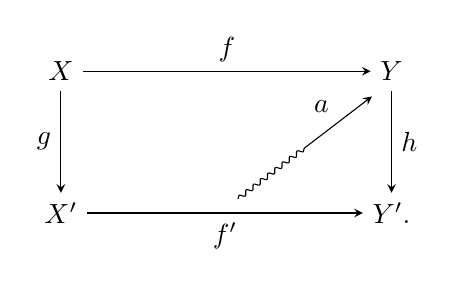
\begin{tikzpicture}[>=stealth,baseline=(current bounding box.center)]
    \node (X)  at (0,1.8) {$X$};
    \node (Y)  at (4.2,1.8) {$Y$};
    \node (Xp) at (0,0) {$X'$};
    \node (Yp) at (4.2,0) {$Y'\mathpunct{.}$};
    \draw[->] (X) -- node[above] {$f$} (Y);
    \draw[->] (X) -- node[left] {$g$} (Xp);
    \draw[->] (Y) -- node[right] {$h$} (Yp);
    \draw[->] (Xp) -- node[below] {$f'$} (Yp);
    \draw[decorate,decoration={snake,amplitude=0.8pt,segment length=3.3pt}]
      (2.25,0.18) -- (3.10,0.83);
    \draw[->] (3.10,0.83) -- node[above left] {$a$} (3.95,1.48);
  \end{tikzpicture}
  \tag{3.1.1.2}
\end{equation}

\VerdierSourcePageBlock{0083}%
\VerdierSemanticAnchor{ch1-3-1-1-additivity}
范畴 $\operatorname{tr}_1(C)$ 是加法范畴。$X\xrightarrow{f}Y$ 与
$X'\xrightarrow{f'}Y'$ 的直和为：

\VerdierSemanticAnchor{ch1-3-1-1-direct-sum}
\begin{equation*}
  X\oplus X'
  \xrightarrow{\left(\begin{smallmatrix}f&0\\0&f'\end{smallmatrix}\right)}
  Y\oplus Y'.
\end{equation*}

\VerdierSemanticAnchor{ch1-3-1-2}
\noindent\textbf{3.1.2.}\quad
设 $X\xrightarrow{f}Y$ 是 $\operatorname{tr}_1(C)$ 的对象。规定：

\VerdierSemanticAnchor{ch1-3-1-2-cone-object}
\begin{equation*}
  c(f)^i=Y^i\oplus X^{i+1},
\end{equation*}

\VerdierSemanticAnchor{ch1-3-1-2-eq1}
\begin{equation}
  d_{c(f)}^i=
  \begin{pmatrix}
    d_Y^i & f^{i+1}\\
    0 & -d_X^{i+1}
  \end{pmatrix}
  \colon Y^i\oplus X^{i+1}\longrightarrow Y^{i+1}\oplus X^{i+2}.
  \tag{3.1.2.1}
\end{equation}

\VerdierSemanticAnchor{ch1-3-1-2-cone-verification}
可验证，这样定义了一个 $C$ 中对象的复形。
\VerdierSemanticAnchor{ch1-3-1-2-cone-name}
此复形记作 $c(f)$，称为态射 $f$ 的\emph{映射锥}。现设

\VerdierSemanticAnchor{ch1-3-1-2-morphism-setup}
\begin{equation*}
  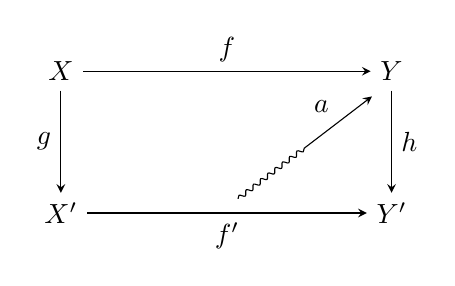
\begin{tikzpicture}[>=stealth,baseline=(current bounding box.center)]
    \node (X)  at (0,1.8) {$X$};
    \node (Y)  at (4.2,1.8) {$Y$};
    \node (Xp) at (0,0) {$X'$};
    \node (Yp) at (4.2,0) {$Y'$};
    \draw[->] (X) -- node[above] {$f$} (Y);
    \draw[->] (X) -- node[left] {$g$} (Xp);
    \draw[->] (Y) -- node[right] {$h$} (Yp);
    \draw[->] (Xp) -- node[below] {$f'$} (Yp);
    \draw[decorate,decoration={snake,amplitude=0.8pt,segment length=3.3pt}]
      (2.25,0.18) -- (3.10,0.83);
    \draw[->] (3.10,0.83) -- node[above left] {$a$} (3.95,1.48);
  \end{tikzpicture}
\end{equation*}
是 $\operatorname{tr}_1(C)$ 的一个态射。规定：

\VerdierSemanticAnchor{ch1-3-1-2-eq2}
\begin{equation}
  c((g,h,a))^i=
  \begin{pmatrix}
    h^i & a^i\\
    0 & g^{i+1}
  \end{pmatrix}
  \colon Y^i\oplus X^{i+1}\longrightarrow Y'^i\oplus X'^{i+1}.
  \tag{3.1.2.2}
\end{equation}

\VerdierSemanticAnchor{ch1-3-1-2-complex-morphism}
这些态射与 $c(f)$ 和 $c(f')$ 的微分交换，因而定义复形态射：

\VerdierSemanticAnchor{ch1-3-1-2-eq3}
\begin{equation}
  c((g,h,a))\colon c(f)\longrightarrow c(f').
  \tag{3.1.2.3}
\end{equation}

\VerdierSemanticAnchor{ch1-3-1-2-cone-functor}
可验证，这样定义了函子
$c\colon\operatorname{tr}_1(C)\longrightarrow\operatorname{comp}(C)$，
称为\emph{映射锥函子}。

\VerdierSemanticAnchor{ch1-3-1-2-s-functor}
以 $s\colon\operatorname{comp}(C)\longrightarrow\operatorname{tr}_1(C)$
表示函子 $X\longmapsto(0\longrightarrow X)$。
\VerdierSemanticAnchor{ch1-3-1-2-phi-setup}
对 $\operatorname{tr}_1(C)$ 的每个对象 $X\xrightarrow{f}Y$，以
$\Phi(f)\colon(X\xrightarrow{f}Y)\longrightarrow s c(f)$ 表示%
\VerdierSourcePageContinue{0084}%
\VerdierSemanticAnchor{ch1-3-1-2-phi-definition-continuation}
$\operatorname{tr}_1(C)$ 的下述态射：

\VerdierSemanticAnchor{ch1-3-1-2-phi-diagram}
\begin{equation*}
  \Phi(f)=(0,p(f),a(f))
  \qquad
  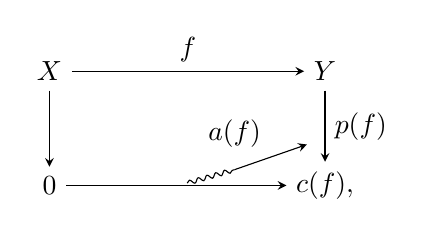
\begin{tikzpicture}[>=stealth,baseline=(current bounding box.center)]
    \node (X)  at (0,1.45) {$X$};
    \node (Y)  at (3.5,1.45) {$Y$};
    \node (Z)  at (0,0) {$0$};
    \node (Cf) at (3.5,0) {$c(f)\mathpunct{,}$};
    \draw[->] (X) -- node[above] {$f$} (Y);
    \draw[->] (X) -- (Z);
    \draw[->] (Y) -- node[right] {$p(f)$} (Cf);
    \draw[->] (Z) -- (Cf);
    \draw[decorate,decoration={snake,amplitude=0.8pt,segment length=3.3pt}]
      (1.75,0.03) -- (2.35,0.20);
    \draw[->] (2.35,0.20) -- node[above left] {$a(f)$} (3.27,0.52);
  \end{tikzpicture}
\end{equation*}

\VerdierSemanticAnchor{ch1-3-1-2-eq4}
\begin{equation}
  \begin{aligned}
    p(f)^i&=
      \begin{pmatrix}
        \operatorname{id}_{Y^i}\\[1mm]
        0
      \end{pmatrix}
      \colon Y^i\longrightarrow Y^i\oplus X^{i+1},\\[2mm]
    a(f)^i&=
      \begin{pmatrix}
        0\\[1mm]
        \operatorname{id}_{X^{i+1}}
      \end{pmatrix}
      \colon X^{i+1}\longrightarrow Y^i\oplus X^{i+1}.
  \end{aligned}
  \tag{3.1.2.4}
\end{equation}

\VerdierSemanticAnchor{ch1-3-1-2-phi-naturality}
直接计算表明，$\Phi$ 是从 $\operatorname{tr}_1(C)$ 的恒等函子到函子 $sc$
的一个函子态射。

\VerdierSemanticAnchor{ch1-3-1-3}
\noindent\textbf{命题 3.1.3.}\quad
\emph{态射 $\Phi$ 使映射锥函子成为函子 $s$ 的左伴随；即对
$\operatorname{tr}_1(C)$ 的任一对象 $X\xrightarrow{f}Y$ 和
$\operatorname{comp}(C)$ 的任一对象 $W$，由态射 $\Phi$ 定义的典范映射}

\VerdierSemanticAnchor{ch1-3-1-3-hom-isomorphism}
\begin{equation*}
  \operatorname{Hom}_{\operatorname{comp}(C)}(c(f),W)
  \longrightarrow
  \operatorname{Hom}_{\operatorname{tr}_1(C)}
    \bigl((X\xrightarrow{f}Y),sW\bigr)
\end{equation*}
\emph{是同构。}

\VerdierSemanticAnchor{ch1-3-1-3-verification}
验证留给读者。
\VerdierSemanticAnchor{ch1-3-1-3-s-fully-faithful}
注意，函子 $s$ 充分忠实，因而函子 $cs$ 典范同构于恒等函子。
\VerdierSemanticAnchor{ch1-3-1-3-cs-identity}
事实上，在所选的函子 $c$ 构造下，函子 $cs$ 等于恒等函子。
\VerdierSemanticAnchor{ch1-3-1-3-adjunction-reformulation}
(3.1.3) 的伴随性质也可表述如下：由函子定义的映射

\VerdierSemanticAnchor{ch1-3-1-3-c-hom-isomorphism}
\begin{equation*}
  c\colon
  \operatorname{Hom}_{\operatorname{tr}_1(C)}
    \bigl((X\xrightarrow{f}Y),sW\bigr)
  \longrightarrow
  \operatorname{Hom}_{\operatorname{comp}(C)}(c(f),W)
\end{equation*}
是同构。

\VerdierSemanticAnchor{ch1-3-1-4}
\noindent\textbf{3.1.4.}\quad
我们将在 $\operatorname{tr}_1(C)$ 中定义同伦的概念。设

\VerdierSemanticAnchor{ch1-3-1-4-homotopy-setup}
\begin{equation*}
  (g,h,a),(g',h',a')\colon
  (X\xrightarrow{f}Y)
  \rightrightarrows
  (X'\xrightarrow{f'}Y')
\end{equation*}%
\VerdierSourcePageContinue{0085}%
\VerdierSemanticAnchor{ch1-3-1-4-homotopy-definition-continuation}
是 $\operatorname{tr}_1(C)$ 的两个态射。连接 $(g,h,a)$ 与
$(g',h',a')$ 的一个\emph{同伦}是三元组 $(b,b',\alpha)$，其中
$b\colon g\rightsquigarrow g'$ 与 $b'\colon h\rightsquigarrow h'$ 是同伦，而

\VerdierSemanticAnchor{ch1-3-1-4-second-order-condition}
\begin{equation*}
  \alpha\colon f'\star b+a'\rightsquigarrow b'\star f+a
\end{equation*}
是二阶同伦 (2.5.12)。

\VerdierSemanticAnchor{ch1-3-1-4-homotopic-morphisms}
若存在连接 $\operatorname{tr}_1(C)$ 中两个态射的同伦，则称它们\emph{同伦}。
\VerdierSemanticAnchor{ch1-3-1-4-equivalence-relation}
“$(g,h,a)$ 与 $(g',h',a')$ 同伦”是一个与态射的直和及复合相容的等价关系。
\VerdierSemanticAnchor{ch1-3-1-4-tr1-homotopy-category}
因此可引入范畴 $\operatorname{Tr}_1(C)$：其对象是
$\operatorname{tr}_1(C)$ 的对象，其态射是 $\operatorname{tr}_1(C)$ 的态射模同伦。

\VerdierSemanticAnchor{ch1-3-1-5}
\noindent\textbf{命题 3.1.5.}\quad
\emph{设
$D,D'\colon (X\xrightarrow{f}Y)\rightrightarrows
(X'\xrightarrow{f'}Y')$ 是 $\operatorname{tr}_1(C)$ 的两个态射。若
$D$ 与 $D'$ 在 $\operatorname{tr}_1(C)$ 中同伦，则 $c(D)$ 与 $c(D')$
在 $\operatorname{comp}(C)$ 中同伦。}

\VerdierSemanticAnchor{ch1-3-1-5-proof-setup}
令 $D=(g,h,a)$、$D'=(g',h',a')$。假定 $D$ 与 $D'$ 在
$\operatorname{tr}_1(C)$ 中同伦。于是存在同伦 $b$ 与 $b'$，使得：

\VerdierSemanticAnchor{ch1-3-1-5-eq1}
\begin{equation}
  \begin{aligned}
    g'-g&=bd+db,\\
    h'-h&=b'd+db'.
  \end{aligned}
  \tag{3.1.5.1}
\end{equation}

（为简化记号，此计算省略了表示各分量次数的上标。）
\VerdierSemanticAnchor{ch1-3-1-5-second-order-homotopy}
此外，存在二阶同伦 $\alpha$，使得
\begin{equation*}
  \alpha d-d\alpha=b'f+a-(f'b+a').
\end{equation*}

\VerdierSemanticAnchor{ch1-3-1-5-cone-homotopy}
直接计算表明
\begin{equation*}
  \begin{pmatrix}
    b' & \alpha\\
    0  & -b
  \end{pmatrix}
\end{equation*}
是连接 $c(D)$ 与 $c(D')$ 的同伦。

\VerdierSemanticAnchor{ch1-3-1-6}
\noindent\textbf{推论 3.1.6.}\quad
\emph{函子}
\begin{equation*}
  c\colon\operatorname{tr}_1(C)\longrightarrow\operatorname{comp}(C)
  \qquad\text{和}\qquad
  s\colon\operatorname{comp}(C)\longrightarrow\operatorname{tr}_1(C)
\end{equation*}
\emph{与 $\operatorname{tr}_1(C)$ 和 $\operatorname{comp}(C)$ 中的同伦相容；
取商后，它们定义仍记作}

\VerdierSemanticAnchor{ch1-3-1-6-descended-functors}
\begin{equation*}
  c\colon\operatorname{Tr}_1(C)\longrightarrow K(C)
  \qquad\text{和}\qquad
  s\colon K(C)\longrightarrow\operatorname{Tr}_1(C)
\end{equation*}
\emph{的函子。}
\VerdierSemanticAnchor{ch1-3-1-6-adjunction}
\emph{函子 $c\colon\operatorname{Tr}_1(C)\longrightarrow K(C)$ 是函子
$s\colon K(C)\longrightarrow\operatorname{Tr}_1(C)$ 的左伴随。}

\VerdierSemanticAnchor{ch1-3-1-6-proof}
这由 (3.1.5) 和 (3.1.3) 形式地推出。

\VerdierSemanticAnchor{ch1-3-1-7}
\noindent\textbf{3.1.7.}\quad
\VerdierSemanticAnchor{ch1-3-1-7-s-prime}
以 $s'\colon\operatorname{comp}(C)\longrightarrow\operatorname{tr}_1(C)$
表示函子 $X\longmapsto(X\longrightarrow 0)$。
\VerdierSemanticAnchor{ch1-3-1-7-comp-translation}
函子 $cs'\colon\operatorname{comp}(C)\longrightarrow\operatorname{comp}(C)$
等于 $\operatorname{comp}(C)$ 的平移函子。
\VerdierSemanticAnchor{ch1-3-1-7-descended-s-prime}
函子 $s'$ 将 $\operatorname{comp}(C)$ 的同伦态射映为
$\operatorname{tr}_1(C)$ 的同伦态射，因而定义函子
$s'\colon K(C)\longrightarrow\operatorname{Tr}_1(C)$，仍以 $s'$ 表示。
\VerdierSemanticAnchor{ch1-3-1-7-k-translation}
函子 $cs'\colon K(C)\longrightarrow K(C)$ 等于 $K(C)$ 的平移函子。

\VerdierSourcePageBlock{0086}%
\VerdierSemanticAnchor{ch1-3-2}
\subsection{映射锥函子的性质}

\VerdierSemanticAnchor{ch1-3-2-1}
\noindent\textbf{3.2.1.}\quad
\VerdierSemanticAnchor{ch1-3-2-1-triangle-definition}
在一个 $\mathbb Z$-范畴中，任何如下形式的图都称为一个\emph{三角}：

\VerdierSemanticAnchor{ch1-3-2-1-eq1}
\begin{equation}
  X\xrightarrow{u}Y\xrightarrow{v}Z\xrightarrow{w}X[1].
  \tag{3.2.1.1}
\end{equation}

\VerdierSemanticAnchor{ch1-3-2-1-notation}
为表示三角 (3.2.1.1)，我们使用记号 $(X,Y,Z,u,v,w)$，或使用图：

\VerdierSemanticAnchor{ch1-3-2-1-eq2}
\begin{equation}
  \begin{tikzpicture}[>=stealth,baseline=(current bounding box.center)]
    \node (X) at (0,0) {$X$};
    \node (Y) at (4.2,0) {$Y\mathpunct{,}$};
    \node (Z) at (2.1,1.65) {$Z$};
    \draw[->] (X) -- node[above] {$u$} (Y);
    \draw[->] (Y) -- node[right] {$v$} (Z);
    \draw[->] (Z) -- node[left] {$w$} (X);
    \draw[line width=0.45pt] (1.91,1.50) -- (1.91,1.67);
  \end{tikzpicture}
  \tag{3.2.1.2}
\end{equation}

\VerdierSemanticAnchor{ch1-3-2-1-pusher-mark}
其中带有短划标记的箭头表示三角中次数为 $1$ 的态射。
\VerdierSemanticAnchor{ch1-3-2-1-triangle-morphism}
设 $(X,Y,Z,u,v,w)$ 和 $(X',Y',Z',u',v',w')$ 是两个三角。
一个\emph{三角的态射}是一个交换图：

\VerdierSemanticAnchor{ch1-3-2-1-eq3}
\begin{equation}
  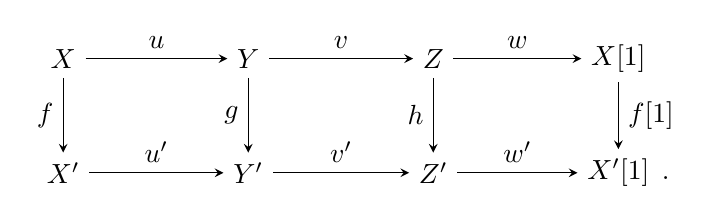
\begin{tikzpicture}[>=stealth,baseline=(current bounding box.center)]
    \node (X)  at (0,1.45) {$X$};
    \node (Y)  at (2.35,1.45) {$Y$};
    \node (Z)  at (4.70,1.45) {$Z$};
    \node (Xs) at (7.05,1.45) {$X[1]$};
    \node (Xp) at (0,0) {$X'$};
    \node (Yp) at (2.35,0) {$Y'$};
    \node (Zp) at (4.70,0) {$Z'$};
    \node (Xps) at (7.05,0) {$X'[1]$};
    \node[anchor=base west,inner sep=0pt,xshift=.08em] at (Xps.base east) {$.$};
    \draw[->] (X) -- node[above] {$u$} (Y);
    \draw[->] (Y) -- node[above] {$v$} (Z);
    \draw[->] (Z) -- node[above] {$w$} (Xs);
    \draw[->] (Xp) -- node[above] {$u'$} (Yp);
    \draw[->] (Yp) -- node[above] {$v'$} (Zp);
    \draw[->] (Zp) -- node[above] {$w'$} (Xps);
    \draw[->] (X) -- node[left] {$f$} (Xp);
    \draw[->] (Y) -- node[left] {$g$} (Yp);
    \draw[->] (Z) -- node[left] {$h$} (Zp);
    \draw[->] (Xs) -- node[right] {$f[1]$} (Xps);
  \end{tikzpicture}
  \tag{3.2.1.3}
\end{equation}

\VerdierSemanticAnchor{ch1-3-2-1-morphism-composition}
三角的态射以显然的方式复合。
\VerdierSemanticAnchor{ch1-3-2-1-triangle-category}
这些三角组成一个范畴。

\VerdierSemanticAnchor{ch1-3-2-2}
\noindent\textbf{3.2.2.}\quad
\VerdierSemanticAnchor{ch1-3-2-2-source-morphism}
设 $X\xrightarrow{f}Y$ 是 $\operatorname{tr}_1(C)$ 的一个对象。下述
$\operatorname{tr}_1(C)$ 的态射（关于 $f$ 函子性）：

\VerdierSemanticAnchor{ch1-3-2-2-eq1}
\begin{equation}
  \begin{tikzpicture}[>=stealth,baseline=(current bounding box.center)]
    \node (X)  at (0,1.35) {$X$};
    \node (Y)  at (3.6,1.35) {$Y$};
    \node (Xp) at (0,0) {$X$};
    \node (Z)  at (3.6,0) {$0$};
    \node[anchor=base west,inner sep=0pt,xshift=.08em] at (Z.base east) {$,$};
    \draw[->] (X) -- node[above] {$f$} (Y);
    \draw[->] (X) -- node[left] {$\operatorname{id}_X$} (Xp);
    \draw[->] (Y) -- (Z);
    \draw[->] (Xp) -- (Z);
  \end{tikzpicture}
  \tag{3.2.2.1}
\end{equation}

\VerdierSemanticAnchor{ch1-3-2-2-cone-application}
经映射锥函子作用后，得到 $\operatorname{comp}(C)$ 中关于
$X\xrightarrow{f}Y$ 函子性的态射 (3.1.7)：

\VerdierSemanticAnchor{ch1-3-2-2-eq2}
\begin{equation}
  q(f)\colon c(f)\longrightarrow X[1].
  \tag{3.2.2.2}
\end{equation}

\VerdierSourcePageBlock{0087}%
\VerdierSemanticAnchor{ch1-3-2-2-dual-morphism}
类似地，$\operatorname{tr}_1(C)$ 的态射：

\VerdierSemanticAnchor{ch1-3-2-2-eq3}
\begin{equation}
  \begin{tikzpicture}[>=stealth,baseline=(current bounding box.center)]
    \node (Z)  at (0,1.35) {$0$};
    \node (Y)  at (3.6,1.35) {$Y$};
    \node (X)  at (0,0) {$X$};
    \node (Yp) at (3.6,0) {$Y$};
    \draw[->] (Z) -- (Y);
    \draw[->] (Z) -- (X);
    \draw[->] (Y) -- node[right] {$\operatorname{id}_Y$} (Yp);
    \draw[->] (X) -- node[above] {$f$} (Yp);
  \end{tikzpicture}
  \tag{3.2.2.3}
\end{equation}

\VerdierSemanticAnchor{ch1-3-2-2-cone-entry-p}
经映射锥函子作用后，得到 $\operatorname{comp}(C)$ 中关于
$X\xrightarrow{f}Y$ 函子性的态射 (3.1.2.4)：

\VerdierSemanticAnchor{ch1-3-2-2-eq4}
\begin{equation}
  p(f)\colon Y\longrightarrow c(f).
  \tag{3.2.2.4}
\end{equation}

\VerdierSemanticAnchor{ch1-3-2-2-comp-triangle}
因此，可对 $\operatorname{tr}_1(C)$ 的每个对象 $X\xrightarrow{f}Y$
配以 $\operatorname{comp}(C)$ 的一个三角：

\VerdierSemanticAnchor{ch1-3-2-2-eq5}
\begin{equation}
  X\xrightarrow{f}Y\xrightarrow{p(f)}c(f)\xrightarrow{q(f)}X[1].
  \tag{3.2.2.5}
\end{equation}

\VerdierSemanticAnchor{ch1-3-2-2-nonfunctoriality}
注意，这个三角并不以函子方式依赖于 $\operatorname{tr}_1(C)$ 的对象
$X\xrightarrow{f}Y$。
\VerdierSemanticAnchor{ch1-3-2-2-morphism-d-setup}
事实上，设
$D=(g,h,a)\colon(X\xrightarrow{f}Y)\longrightarrow
(X'\xrightarrow{f'}Y')$
是 $\operatorname{tr}_1(C)$ 的一个态射。于是得到图：

\VerdierSemanticAnchor{ch1-3-2-2-eq6}
\begin{equation}
  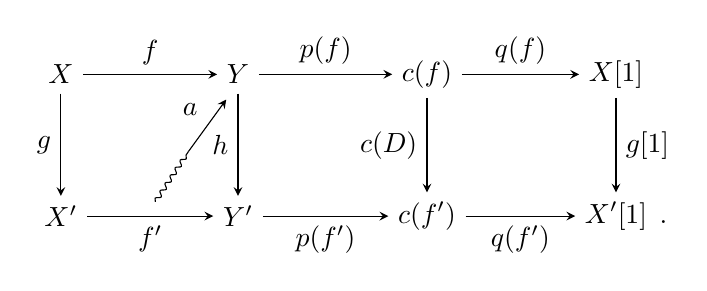
\begin{tikzpicture}[>=stealth,baseline=(current bounding box.center)]
    \node (X)   at (0,1.8) {$X$};
    \node (Y)   at (2.25,1.8) {$Y$};
    \node (C)   at (4.65,1.8) {$c(f)$};
    \node (Xs)  at (7.05,1.8) {$X[1]$};
    \node (Xp)  at (0,0) {$X'$};
    \node (Yp)  at (2.25,0) {$Y'$};
    \node (Cp)  at (4.65,0) {$c(f')$};
    \node (Xps) at (7.05,0) {$X'[1]$};
    \node[anchor=base west,inner sep=0pt,xshift=.08em] at (Xps.base east) {$.$};
    \draw[->] (X) -- node[above] {$f$} (Y);
    \draw[->] (Y) -- node[above] {$p(f)$} (C);
    \draw[->] (C) -- node[above] {$q(f)$} (Xs);
    \draw[->] (Xp) -- node[below] {$f'$} (Yp);
    \draw[->] (Yp) -- node[below] {$p(f')$} (Cp);
    \draw[->] (Cp) -- node[below] {$q(f')$} (Xps);
    \draw[->] (X) -- node[left] {$g$} (Xp);
    \draw[->] (Y) -- node[left] {$h$} (Yp);
    \draw[->] (C) -- node[left] {$c(D)$} (Cp);
    \draw[->] (Xs) -- node[right] {$g[1]$} (Xps);
    \draw[decorate,decoration={snake,amplitude=0.8pt,segment length=3.3pt}]
      (1.20,0.18) -- (1.62,0.82);
    \draw[->] (1.62,0.82) -- node[above left] {$a$} (2.10,1.48);
  \end{tikzpicture}
  \tag{3.2.2.6}
\end{equation}

\VerdierSemanticAnchor{ch1-3-2-2-square-commutativity}
由于态射 $p(f)$ 和 $q(f)$ 关于 $f$ 函子性，此图的后两个方块交换，
而第一个方块只在同伦意义下交换。
\VerdierSemanticAnchor{ch1-3-2-2-quotient-triangle}
对同伦取商后，可对 $\operatorname{Tr}_1(C)$ 的每个对象
$X\xrightarrow{f}Y$ 配以 $K(C)$ 的一个三角：

\VerdierSemanticAnchor{ch1-3-2-2-eq7}
\begin{equation}
  X\xrightarrow{\dot f}Y\xrightarrow{\dot p(f)}c(f)
  \xrightarrow{\dot q(f)}X[1]
  \tag{3.2.2.7}
\end{equation}

\VerdierSemanticAnchor{ch1-3-2-2-homotopy-class-notation}
它以函子方式依赖于 $X\xrightarrow{f}Y$。（这里 $\dot f$、
$\dot p(f)$、$\dot q(f)$ 分别表示态射 $f$、$p(f)$、$q(f)$ 的同伦类。）
\VerdierSemanticAnchor{ch1-3-2-2-triangle-functor}
于是得到一个从范畴 $\operatorname{Tr}_1(C)$ 到 $K(C)$ 中三角所成范畴的函子。

\VerdierSourcePageBlock{0088}%
\VerdierSemanticAnchor{ch1-3-2-3}
\noindent\textbf{3.2.3.}\quad
\VerdierSemanticAnchor{ch1-3-2-3-translation-automorphism}
$\operatorname{comp}(C)$ 的平移自同构自然延拓为自同构
$T\colon\operatorname{tr}_1(C)\longrightarrow\operatorname{tr}_1(C)$：

\VerdierSemanticAnchor{ch1-3-2-3-eq1}
\begin{equation}
  \begin{aligned}
    T\bigl(X\xrightarrow{f}Y\bigr)
      &=X[1]\xrightarrow{f[1]}Y[1],\\
    T((g,h,a))&=(g[1],h[1],-a[1]).
  \end{aligned}
  \tag{3.2.3.1}
\end{equation}

\VerdierSemanticAnchor{ch1-3-2-3-cone-z-functor}
于是，通过定义同构
\VerdierSemanticAnchor{ch1-3-2-3-psi-isomorphism}
$\Psi(f)\colon c(f[1])\xrightarrow{\sim}c(f)[1]$，使映射锥函子成为一个
$\mathbb Z$-函子 (1.5.2)：

\VerdierSemanticAnchor{ch1-3-2-3-eq2}
\begin{equation}
  \Psi(f)^i=
  \begin{pmatrix}
    \operatorname{id}_{Y^{i+1}} & 0\\
    0 & -\operatorname{id}_{X^{i+2}}
  \end{pmatrix}
  \colon Y^{i+1}\oplus X^{i+2}
  \longrightarrow Y^{i+1}\oplus X^{i+2}.
  \tag{3.2.3.2}
\end{equation}

\VerdierSemanticAnchor{ch1-3-2-3-reader-verification}
读者将验证 (3.2.3.2) 确实定义了复形的同构，并证明下述命题：

\VerdierSemanticAnchor{ch1-3-2-4}
\noindent\textbf{命题 3.2.4.}\quad
\VerdierSemanticAnchor{ch1-3-2-4-zero-source}
\emph{当 $f=0\longrightarrow Y$ 时，典范同构}
\begin{equation*}
  c(f[n])\xrightarrow{\sim}c(f)[n]
\end{equation*}
\emph{就是 $Y[n]$ 的恒等映射。当 $f=X\longrightarrow0$ 时，典范同构}
\VerdierSemanticAnchor{ch1-3-2-4-zero-target}
\begin{equation*}
  c(f[n])\xrightarrow{\sim}c(f)[n]
\end{equation*}
\emph{就是同构}
\begin{equation*}
  X[n+1]\xrightarrow{(-1)^n\operatorname{id}_{X[n+1]}}X[n+1].
\end{equation*}

\VerdierSemanticAnchor{ch1-3-2-5}
\noindent\textbf{3.2.5.}\quad
设 $X\xrightarrow{f}Y$ 是 $\operatorname{tr}_1(C)$ 的一个对象。
可对其配以 $\operatorname{comp}(C)$ 的一个三角：

\VerdierSemanticAnchor{ch1-3-2-5-triangle}
\VerdierSemanticAnchor{ch1-3-2-5-eq1}
\begin{equation}
  Y\xrightarrow{p(f)}c(f)\xrightarrow{q(f)}X[1]
  \xrightarrow{f[1]}Y[1].
  \tag{3.2.5.1}
\end{equation}

\VerdierSemanticAnchor{ch1-3-2-5-composite}
态射 $q(f)p(f)\colon Y\longrightarrow X[1]$ 是下述态射在映射锥函子下的像：

\VerdierSemanticAnchor{ch1-3-2-5-cone-morphism-diagram}
\begin{equation*}
  \begin{tikzpicture}[>=stealth,baseline=(current bounding box.center)]
    \node (Z1) at (0,1.45) {$0$};
    \node (Y)  at (3.5,1.45) {$Y$};
    \node (X)  at (0,0) {$X$};
    \node (Z2) at (3.5,0) {$0$};
    \node[anchor=base west,inner sep=0pt,xshift=.08em] at (Z2.base east) {$.$};
    \draw[->] (Z1) -- (Y);
    \draw[->] (Z1) -- (X);
    \draw[->] (Y) -- (Z2);
    \draw[->] (X) -- (Z2);
  \end{tikzpicture}
\end{equation*}%
\VerdierSourcePageContinue{0089}%
\VerdierSemanticAnchor{ch1-3-2-5-composite-zero-conclusion}
因此它为零。由映射锥函子的伴随性质 (3.1.3)，存在唯一态射：

\VerdierSemanticAnchor{ch1-3-2-5-eq2}
\begin{equation}
  J\colon c(p(f))\longrightarrow X[1],
  \tag{3.2.5.2}
\end{equation}

\noindent 使得下图交换：

\VerdierSemanticAnchor{ch1-3-2-5-eq3}
\VerdierSemanticAnchor{ch1-3-2-5-j-comparison-diagram}
\begin{equation}
  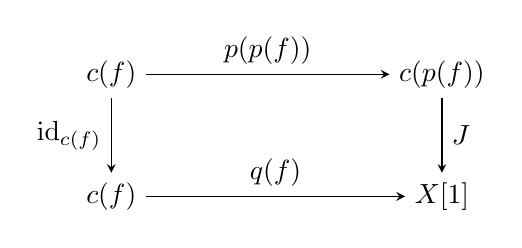
\begin{tikzpicture}[>=stealth,baseline=(current bounding box.center)]
    \node (Cf1) at (0,1.55) {$c(f)$};
    \node (Cpf) at (4.2,1.55) {$c(p(f))$};
    \node (Cf2) at (0,0) {$c(f)$};
    \node (Xs)  at (4.2,0) {$X[1]$};
    \draw[->] (Cf1) -- node[above] {$p(p(f))$} (Cpf);
    \draw[->] (Cf1) -- node[left] {$\operatorname{id}_{c(f)}$} (Cf2);
    \draw[->] (Cpf) -- node[right] {$J$} (Xs);
    \draw[->] (Cf2) -- node[above] {$q(f)$} (Xs);
  \end{tikzpicture}
  \tag{3.2.5.3}
\end{equation}

\noindent 并且 $Ja(p(f))=0$ (3.1.2.4)。

\VerdierSemanticAnchor{ch1-3-2-6}
\noindent\textbf{命题 3.2.6.}\quad
\VerdierSemanticAnchor{ch1-3-2-6-a}
\emph{a) 态射 $J$ 是同伦等价；即它在同伦意义下是同构。}

\VerdierSemanticAnchor{ch1-3-2-6-b}
\emph{b) 下图}

\VerdierSemanticAnchor{ch1-3-2-6-eq1}
\begin{equation}
  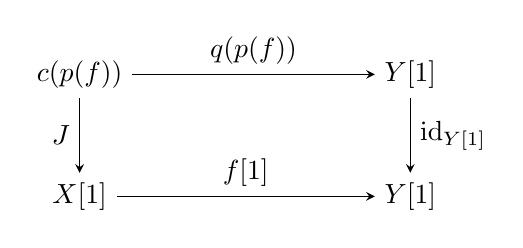
\begin{tikzpicture}[>=stealth,baseline=(current bounding box.center)]
    \node (Cpf) at (0,1.55) {$c(p(f))$};
    \node (Ys1) at (4.2,1.55) {$Y[1]$};
    \node (Xs)  at (0,0) {$X[1]$};
    \node (Ys2) at (4.2,0) {$Y[1]$};
    \draw[->] (Cpf) -- node[above] {$q(p(f))$} (Ys1);
    \draw[->] (Cpf) -- node[left] {$J$} (Xs);
    \draw[->] (Ys1) -- node[right] {$\operatorname{id}_{Y[1]}$} (Ys2);
    \draw[->] (Xs) -- node[above] {$f[1]$} (Ys2);
  \end{tikzpicture}
  \tag{3.2.6.1}
\end{equation}

\noindent\emph{在同伦意义下反交换。}

\VerdierSemanticAnchor{ch1-3-2-7}
\noindent\textbf{3.2.7. 证明。}\quad
\VerdierSemanticAnchor{ch1-3-2-7-h-construction}
首先构造一个态射 $H\colon X[1]\longrightarrow c(p(f))$。
\VerdierSemanticAnchor{ch1-3-2-7-representing-functors}
为此，只需构造这两个对象所表示的两个函子之间的态射。设 $W$ 是
$\operatorname{comp}(C)$ 的一个对象。
\VerdierSemanticAnchor{ch1-3-2-7-pair}
由映射锥函子的伴随性质 (3.1.3)，从 $c(p(f))$ 到 $W$ 的一个态射无非是
一对 $(u,a)$，其中 $u\colon c(f)\longrightarrow W$ 是复形态射，
$a\colon0\rightsquigarrow up(f)$ 是一个同伦。
\VerdierSemanticAnchor{ch1-3-2-7-triple}
再次使用 (3.1.3)，可见从 $c(p(f))$ 到 $W$ 的一个态射就是一个三元组
\begin{equation*}
  \bigl(m\colon Y\longrightarrow W,\quad
  a\colon0\rightsquigarrow m,\quad
  b\colon0\rightsquigarrow mf\bigr).
\end{equation*}
对这个三元组配以下图：

\VerdierSemanticAnchor{ch1-3-2-7-eq1}
\begin{equation}
  \begin{gathered}
    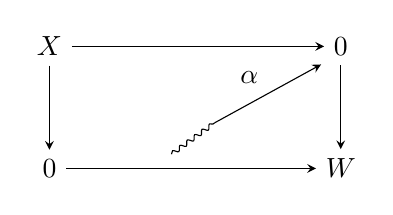
\begin{tikzpicture}[>=stealth,baseline=(current bounding box.center)]
      \node (X)  at (0,1.55) {$X$};
      \node (Z1) at (3.7,1.55) {$0$};
      \node (Z2) at (0,0) {$0$};
      \node (W)  at (3.7,0) {$W$};
      \draw[->] (X) -- (Z1);
      \draw[->] (X) -- (Z2);
      \draw[->] (Z1) -- (W);
      \draw[->] (Z2) -- (W);
      \draw[decorate,decoration={snake,amplitude=0.8pt,segment length=3.3pt}]
        (1.55,0.18) -- (2.10,0.58);
      \draw[->] (2.10,0.58) -- node[above left] {$\alpha$} (3.45,1.32);
    \end{tikzpicture}
    \qquad \alpha=b-a\star f ,
  \end{gathered}
  \tag{3.2.7.1}
\end{equation}%
\VerdierSourcePageContinue{0090}%
\VerdierSemanticAnchor{ch1-3-2-7-representing-functor-continuation}
即由 (3.1.3) 和 (3.1.7) 得到一个从 $X[1]$ 到 $W$ 的态射。这样，我们以
关于 $W$ 函子性的方式，把从 $c(p(f))$ 到 $W$ 的每个态射配到从 $X[1]$
到 $W$ 的一个态射，从而定义了态射
\VerdierSemanticAnchor{ch1-3-2-7-h-defined}
$H\colon X[1]\longrightarrow c(p(f))$。

为证明命题 (3.2.6) 的 a) 部分，只需证明：

\VerdierSemanticAnchor{ch1-3-2-7-eq2}
\begin{equation}
  \textit{态射 }JH\colon X[1]\longrightarrow X[1]
  \textit{ 是恒等态射。}
  \tag{3.2.7.2}
\end{equation}

\VerdierSemanticAnchor{ch1-3-2-7-eq3}
\begin{equation}
  \textit{态射 }HJ\colon c(p(f))\longrightarrow c(p(f))
  \textit{ 同伦于恒等态射。}
  \tag{3.2.7.3}
\end{equation}

为证明命题 (3.2.6) 的 b) 部分，还只需证明：

\VerdierSemanticAnchor{ch1-3-2-7-eq4}
\begin{equation}
  \begin{gathered}
    \textit{下图：}\\[0.35em]
    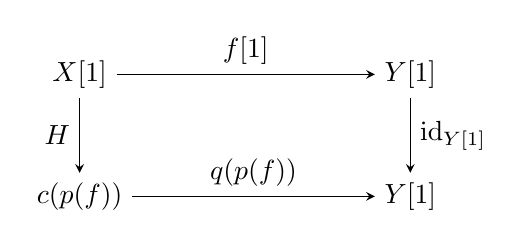
\begin{tikzpicture}[>=stealth,baseline=(current bounding box.center)]
      \node (Xs)  at (0,1.55) {$X[1]$};
      \node (Ys1) at (4.2,1.55) {$Y[1]$};
      \node (Cpf) at (0,0) {$c(p(f))$};
      \node (Ys2) at (4.2,0) {$Y[1]$};
      \draw[->] (Xs) -- node[above] {$f[1]$} (Ys1);
      \draw[->] (Xs) -- node[left] {$H$} (Cpf);
      \draw[->] (Ys1) -- node[right] {$\operatorname{id}_{Y[1]}$} (Ys2);
      \draw[->] (Cpf) -- node[above] {$q(p(f))$} (Ys2);
    \end{tikzpicture}\\[-0.15em]
    \textit{反交换。}
  \end{gathered}
  \tag{3.2.7.4}
\end{equation}

\VerdierSemanticAnchor{ch1-3-2-8}
\noindent\textbf{3.2.8. 断言 (3.2.7.2) 的证明。}\quad
\VerdierSemanticAnchor{ch1-3-2-8-jh-identity-proof}
证明态射 $JH\colon X[1]\longrightarrow X[1]$ 是恒等态射。为此，只需说明
态射 $JH$ 在由 $X[1]$ 表示的函子上诱导恒等自同态。
\VerdierSemanticAnchor{ch1-3-2-8-represented-hom-functor}
由 (3.1.3) 和 (3.1.7)，函子
\begin{equation*}
  W\longmapsto
  \operatorname{Hom}_{\operatorname{comp}(C)}(X[1],W)
\end{equation*}
就是函子：

\VerdierSemanticAnchor{ch1-3-2-8-eq1}
\begin{equation}
  W\longmapsto
  \left\{\,
  \vcenter{\hbox{%
    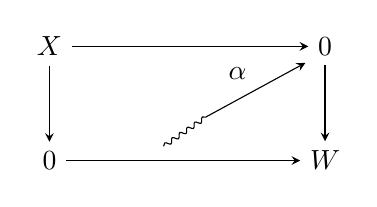
\begin{tikzpicture}[>=stealth,baseline=(current bounding box.center)]
      \node (X)  at (0,1.45) {$X$};
      \node (Z1) at (3.5,1.45) {$0$};
      \node (Z2) at (0,0) {$0$};
      \node (W)  at (3.5,0) {$W$};
      \draw[->] (X) -- (Z1);
      \draw[->] (X) -- (Z2);
      \draw[->] (Z1) -- (W);
      \draw[->] (Z2) -- (W);
      \draw[decorate,decoration={snake,amplitude=0.8pt,segment length=3.3pt}]
        (1.45,0.18) -- (2.00,0.56);
      \draw[->] (2.00,0.56) -- node[above left] {$\alpha$} (3.25,1.24);
    \end{tikzpicture}%
  }}\,\right\}.
  \tag{3.2.8.1}
\end{equation}

\VerdierSemanticAnchor{ch1-3-2-8-cpf-represented-functor}
另一方面，由 (3.2.7)，$\operatorname{comp}(C)$ 的对象 $c(p(f))$ 表示函子：

\VerdierSemanticAnchor{ch1-3-2-8-eq2}
\begin{equation}
  W\longmapsto
  \left\{\,
  \bigl(m\colon Y\longrightarrow W,\quad
  a\colon0\rightsquigarrow m,\quad
  b\colon0\rightsquigarrow mf\bigr)
  \,\right\}.
  \tag{3.2.8.2}
\end{equation}%
\VerdierSourcePageContinue{0091}%
\VerdierSemanticAnchor{ch1-3-2-8-j-induced-functorial-map}
态射 $J\colon c(p(f))\longrightarrow X[1]$ 对应于如下函子态射，
这一点可立即验证：

\VerdierSemanticAnchor{ch1-3-2-8-eq3}
\begin{equation}
  \begin{gathered}
    D=
    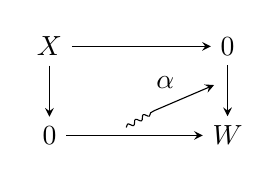
\begin{tikzpicture}[>=stealth,baseline=(current bounding box.center),
      scale=0.78,every node/.style={}]
      \node (X)  at (0,1.45) {$X$};
      \node (Z1) at (2.9,1.45) {$0$};
      \node (Z2) at (0,0) {$0$};
      \node (W)  at (2.9,0) {$W$};
      \draw[->] (X) -- (Z1);
      \draw[->] (X) -- (Z2);
      \draw[->] (Z1) -- (W);
      \draw[->] (Z2) -- (W);
      \draw[decorate,decoration={snake,amplitude=0.8pt,segment length=3.3pt}]
        (1.25,0.13) -- (1.70,0.40);
      \draw[->] (1.70,0.40) -- node[above left] {$\alpha$} (2.68,0.82);
    \end{tikzpicture}
    \quad\longmapsto\quad
    JD=\bigl(0\colon Y\longrightarrow W,\;
      0\colon0\rightsquigarrow0,\;
      \alpha\colon0\rightsquigarrow0\bigr).
  \end{gathered}
  \tag{3.2.8.3}
\end{equation}

\VerdierSemanticAnchor{ch1-3-2-8-h-induced-functorial-map}
依定义 (3.2.7)，态射 $H\colon X[1]\longrightarrow c(p(f))$
对应于如下函子态射：

\VerdierSemanticAnchor{ch1-3-2-8-eq4}
\begin{equation}
  \begin{aligned}
    t={}&\bigl(m\colon Y\longrightarrow W,\;
      a\colon0\rightsquigarrow m,\;
      b\colon0\rightsquigarrow mf\bigr)\\[-0.2em]
    &\longmapsto\quad Ht=
    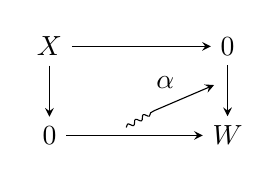
\begin{tikzpicture}[>=stealth,baseline=(current bounding box.center),
      scale=0.78,every node/.style={}]
      \node (X)  at (0,1.45) {$X$};
      \node (Z1) at (2.9,1.45) {$0$};
      \node (Z2) at (0,0) {$0$};
      \node (W)  at (2.9,0) {$W$};
      \draw[->] (X) -- (Z1);
      \draw[->] (X) -- (Z2);
      \draw[->] (Z1) -- (W);
      \draw[->] (Z2) -- (W);
      \draw[decorate,decoration={snake,amplitude=0.8pt,segment length=3.3pt}]
        (1.25,0.13) -- (1.70,0.40);
      \draw[->] (1.70,0.40) -- node[above left] {$\alpha$} (2.68,0.82);
    \end{tikzpicture}
    ,\qquad \alpha=b-a\star f.
  \end{aligned}
  \tag{3.2.8.4}
\end{equation}

\VerdierSemanticAnchor{ch1-3-2-8-composite-identity}
这两个函子态射的复合确为恒等，从而证明了断言 (3.2.7.2)。

\VerdierSemanticAnchor{ch1-3-2-9}
\noindent\textbf{3.2.9. 断言 (3.2.7.3) 的证明。}\quad
\VerdierSemanticAnchor{ch1-3-2-9-hj-functorial-map}
由 (3.2.8)，态射
$HJ\colon c(p(f))\longrightarrow c(p(f))$ 对应于如下函子态射：

\VerdierSemanticAnchor{ch1-3-2-9-eq1}
\begin{equation}
  \begin{aligned}
    t={}&\bigl(m\colon Y\longrightarrow W,\;
      a\colon0\rightsquigarrow m,\;
      b\colon0\rightsquigarrow mf\bigr)
      \longmapsto HJt\\
    ={}&\bigl(0\colon Y\longrightarrow W,\;
      0\colon0\rightsquigarrow0,\;
      b-a\star f\colon0\rightsquigarrow0\bigr)
  \end{aligned}
  \tag{3.2.9.1}
\end{equation}
因此：

\VerdierSemanticAnchor{ch1-3-2-9-eq2}
\begin{equation}
  t-HJt=\bigl(m\colon Y\longrightarrow W,\;
    a\colon0\rightsquigarrow m,\;
    a\star f\colon0\rightsquigarrow mf\bigr).
  \tag{3.2.9.2}
\end{equation}

\VerdierSemanticAnchor{ch1-3-2-9-null-homotopy-reduction}
为证明断言 (3.2.7.3)，只需证明每个形如
$\bigl(m\colon Y\longrightarrow W,\;a\colon0\rightsquigarrow m,\;
a\star f\colon0\rightsquigarrow mf\bigr)$ 的三元组，都对应于一个从
$c(p(f))$ 到 $W$ 的同伦于零的态射。利用 (3.1.3)，这样的三元组定义一个态射：

\VerdierSemanticAnchor{ch1-3-2-9-eq3}
\begin{equation}
  v\colon c(f)\longrightarrow W,
  \qquad
  v=\bigl(m\colon Y\longrightarrow W,\;
    a\star f\colon0\rightsquigarrow mf\bigr)
  \tag{3.2.9.3}
\end{equation}
以及一个同伦：

\VerdierSemanticAnchor{ch1-3-2-9-eq4}
\begin{equation}
  a\colon0\rightsquigarrow vp(f)=m,
  \tag{3.2.9.4}
\end{equation}%
\VerdierSourcePageContinue{0092}%
\VerdierSemanticAnchor{ch1-3-2-9-eq5}
从而得到图：
\begin{equation}
  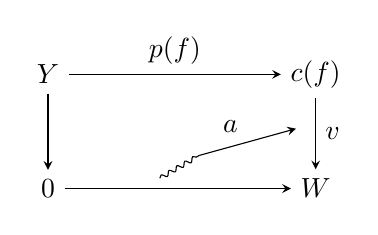
\begin{tikzpicture}[>=stealth,baseline=(current bounding box.center)]
    \node (Y)  at (0,1.45) {$Y$};
    \node (Cf) at (3.4,1.45) {$c(f)$};
    \node (Z)  at (0,0) {$0$};
    \node (W)  at (3.4,0) {$W$};
    \draw[->] (Y) -- node[above] {$p(f)$} (Cf);
    \draw[->] (Y) -- (Z);
    \draw[->] (Cf) -- node[right] {$v$} (W);
    \draw[->] (Z) -- (W);
    \draw[decorate,decoration={snake,amplitude=0.8pt,segment length=3.3pt}]
      (1.42,0.13) -- (1.92,0.42);
    \draw[->] (1.92,0.42) -- node[above left] {$a$} (3.15,0.76);
  \end{tikzpicture}
  \tag{3.2.9.5}
\end{equation}

\VerdierSemanticAnchor{ch1-3-2-9-n-morphism}
依 (3.1.3)，此图定义了与三元组
$\bigl(m\colon Y\longrightarrow W,\;a\colon0\rightsquigarrow m,\;
a\star f\colon0\rightsquigarrow mf\bigr)$ 相对应的态射
$n\colon c(p(f))\longrightarrow W$。为证明态射 $n$ 同伦于零，依 (3.1.5)，
只需证明图 (3.2.9.5) 是 $\operatorname{tr}_1(C)$ 中一个同伦于零的态射；
为此，只需证明存在同伦 $\beta\colon0\rightsquigarrow v$，使得
$\beta\star p(f)=a$。态射 $v\colon c(f)\longrightarrow W$ 的分量为：

\VerdierSemanticAnchor{ch1-3-2-9-eq6}
\begin{equation}
  v^i=(m^i,a^if^{i+1})\colon Y^i\oplus X^{i+1}\longrightarrow W^i
  \tag{3.2.9.6}
\end{equation}
而且可立即验证，分量为

\VerdierSemanticAnchor{ch1-3-2-9-eq7}
\begin{equation}
  \beta^i=(a^i,0)\colon Y^{i+1}\oplus X^{i+2}\longrightarrow W^i
  \tag{3.2.9.7}
\end{equation}

\VerdierSemanticAnchor{ch1-3-2-9-conclusion}
的同伦 $\beta$ 联结 $0$ 与 $v$，且满足 $\beta\star p(f)=a$。
这就完成了断言 (3.2.7.3) 的证明。

\VerdierSemanticAnchor{ch1-3-2-10}
\noindent\textbf{3.2.10. 断言 (3.2.7.4) 的证明。}\quad
\VerdierSemanticAnchor{ch1-3-2-10-y1-represented-functor}
对象 $Y[1]$ 表示函子：

\VerdierSemanticAnchor{ch1-3-2-10-eq1}
\begin{equation}
  W\longmapsto
  \left\{\,
  \vcenter{\hbox{%
    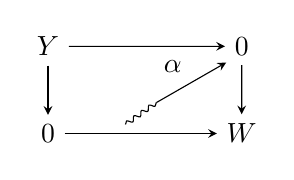
\begin{tikzpicture}[>=stealth,baseline=(current bounding box.center),scale=0.82,
      every node/.style={}]
      \node (Y) at (0,1.35) {$Y$};
      \node (ZT) at (3.0,1.35) {$0$};
      \node (ZB) at (0,0) {$0$};
      \node (W) at (3.0,0) {$W$};
      \draw[->] (Y) -- (ZT);
      \draw[->] (Y) -- (ZB);
      \draw[->] (ZT) -- (W);
      \draw[->] (ZB) -- (W);
      \draw[decorate,decoration={snake,amplitude=0.8pt,segment length=3.3pt}]
        (1.20,0.14) -- (1.68,0.48);
      \draw[->] (1.68,0.48) -- node[above left] {$\alpha$} (2.76,1.10);
    \end{tikzpicture}%
  }}\,\right\}.
  \tag{3.2.10.1}
\end{equation}

\VerdierSemanticAnchor{ch1-3-2-10-f1-functorial-map}
而态射 $f[1]\colon X[1]\longrightarrow Y[1]$ 表示函子态射：

\VerdierSemanticAnchor{ch1-3-2-10-eq2}
\begin{equation}
  \begin{gathered}
    D=
    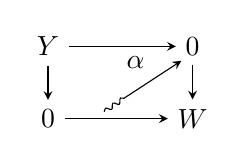
\begin{tikzpicture}[>=stealth,baseline=(current bounding box.center),scale=0.68,
      every node/.style={}]
      \node (Y) at (0,1.35) {$Y$};
      \node (ZT) at (2.7,1.35) {$0$};
      \node (ZB) at (0,0) {$0$};
      \node (W) at (2.7,0) {$W$};
      \draw[->] (Y) -- (ZT); \draw[->] (Y) -- (ZB);
      \draw[->] (ZT) -- (W); \draw[->] (ZB) -- (W);
      \draw[decorate,decoration={snake,amplitude=0.8pt,segment length=3.3pt}]
        (1.05,0.13) -- (1.48,0.42);
      \draw[->] (1.48,0.42) -- node[above left] {$\alpha$} (2.49,1.08);
    \end{tikzpicture}
    \quad\longmapsto\quad f[1]D=
    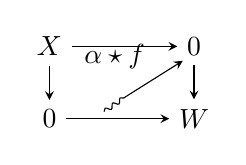
\begin{tikzpicture}[>=stealth,baseline=(current bounding box.center),scale=0.68,
      every node/.style={}]
      \node (X) at (0,1.35) {$X$};
      \node (ZT) at (2.7,1.35) {$0$};
      \node (ZB) at (0,0) {$0$};
      \node (W) at (2.7,0) {$W$};
      \draw[->] (X) -- (ZT); \draw[->] (X) -- (ZB);
      \draw[->] (ZT) -- (W); \draw[->] (ZB) -- (W);
      \draw[decorate,decoration={snake,amplitude=0.8pt,segment length=3.3pt}]
        (1.02,0.13) -- (1.44,0.42);
      \draw[->] (1.44,0.42) -- node[above left] {$\alpha\star f$} (2.49,1.08);
    \end{tikzpicture}
  \end{gathered}
  \tag{3.2.10.2}
\end{equation}%
\VerdierSourcePageContinue{0093}%
\begingroup
\setlength{\abovedisplayskip}{5pt plus 2pt minus 2pt}%
\setlength{\belowdisplayskip}{5pt plus 2pt minus 2pt}%
\VerdierSemanticAnchor{ch1-3-2-10-qpf-functorial-map}
同样，态射 $q(p(f))\colon c(p(f))\longrightarrow Y[1]$
表示函子态射：

\VerdierSemanticAnchor{ch1-3-2-10-eq3}
\begin{equation}
  \begin{gathered}
    D=
    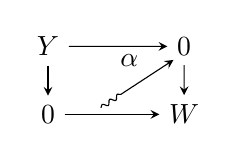
\begin{tikzpicture}[>=stealth,baseline=(current bounding box.center),scale=0.64,
      every node/.style={}]
      \node (Y) at (0,1.35) {$Y$};
      \node (ZT) at (2.7,1.35) {$0$};
      \node (ZB) at (0,0) {$0$};
      \node (W) at (2.7,0) {$W$};
      \draw[->] (Y) -- (ZT); \draw[->] (Y) -- (ZB);
      \draw[->] (ZT) -- (W); \draw[->] (ZB) -- (W);
      \draw[decorate,decoration={snake,amplitude=0.8pt,segment length=3.3pt}]
        (1.05,0.13) -- (1.48,0.42);
      \draw[->] (1.48,0.42) -- node[above left] {$\alpha$} (2.49,1.08);
    \end{tikzpicture}
    \quad\longmapsto\quad
    q(p(f))D=
    \bigl(0\colon Y\longrightarrow W,\;
      \alpha\colon0\rightsquigarrow0,\;
      0\colon0\rightsquigarrow0\bigr).
  \end{gathered}
  \tag{3.2.10.3}
\end{equation}

\VerdierSemanticAnchor{ch1-3-2-10-conclusion}
因此，利用 (3.2.8.4)，为证明 (3.2.7.4)，只需注意，对每个图
\[
  D=
  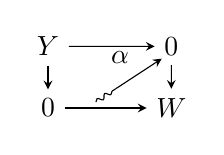
\begin{tikzpicture}[>=stealth,baseline=(current bounding box.center),scale=0.58,
    every node/.style={}]
    \node (Y) at (0,1.35) {$Y$};
    \node (ZT) at (2.7,1.35) {$0$};
    \node (ZB) at (0,0) {$0$};
    \node (W) at (2.7,0) {$W$};
    \draw[->] (Y) -- (ZT); \draw[->] (Y) -- (ZB);
    \draw[->] (ZT) -- (W); \draw[->] (ZB) -- (W);
    \draw[decorate,decoration={snake,amplitude=0.8pt,segment length=3.3pt}]
      (1.05,0.13) -- (1.48,0.42);
    \draw[->] (1.48,0.42) -- node[above left] {$\alpha$} (2.49,1.08);
  \end{tikzpicture}
  \qquad Hq(p(f))D+f[1]D=0.
\]

\VerdierSemanticAnchor{ch1-3-2-11}
\noindent\textbf{3.2.11.}
\VerdierSemanticAnchor{ch1-3-2-11-composable-morphisms}
设 $X\xrightarrow{f}Y\xrightarrow{g}Z$ 是 $\operatorname{comp}(C)$ 中
两个态射。置 $gf=h$。利用这些数据，可以构造两个交换图：

\VerdierSemanticAnchor{ch1-3-2-11-eq1}
\begin{equation}
  \begin{gathered}
  D=
  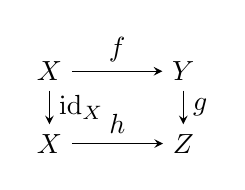
\begin{tikzpicture}[>=stealth,baseline=(current bounding box.center),scale=0.68,
    every node/.style={}]
    \node (X1) at (0,1.35) {$X$}; \node (Y) at (2.5,1.35) {$Y$};
    \node (X2) at (0,0) {$X$}; \node (Z) at (2.5,0) {$Z$};
    \draw[->] (X1) -- node[above] {$f$} (Y);
    \draw[->] (X1) -- node[right] {$\operatorname{id}_X$} (X2);
    \draw[->] (Y) -- node[right] {$g$} (Z);
    \draw[->] (X2) -- node[above] {$h$} (Z);
  \end{tikzpicture},
  \qquad
  D'=
  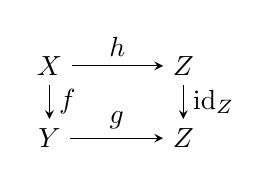
\begin{tikzpicture}[>=stealth,baseline=(current bounding box.center),scale=0.68,
    every node/.style={}]
    \node (X) at (0,1.35) {$X$}; \node (Z1) at (2.5,1.35) {$Z$};
    \node (Y) at (0,0) {$Y$}; \node (Z2) at (2.5,0) {$Z$};
    \draw[->] (X) -- node[above] {$h$} (Z1);
    \draw[->] (X) -- node[right] {$f$} (Y);
    \draw[->] (Z1) -- node[right] {$\operatorname{id}_Z$} (Z2);
    \draw[->] (Y) -- node[above] {$g$} (Z2);
  \end{tikzpicture}
  \end{gathered}
  \tag{3.2.11.1}
\end{equation}

\VerdierSemanticAnchor{ch1-3-2-11-cone-images}
我们把它们解释为 $\operatorname{tr}_1(C)$ 的态射。因此，应用映射锥函子，
得到两个图：
\[
  c(f)\xrightarrow{c(D)}c(h)\xrightarrow{c(D')}c(g)
\]

\VerdierSemanticAnchor{ch1-3-2-11-eq2}
\begin{equation}
  I=
  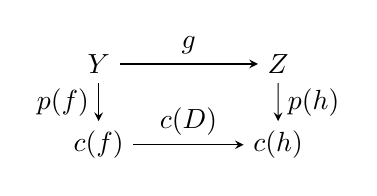
\begin{tikzpicture}[>=stealth,baseline=(current bounding box.center),scale=0.76,
    every node/.style={}]
    \node (Y) at (0,1.35) {$Y$}; \node (Z) at (3.0,1.35) {$Z$};
    \node (Cf) at (0,0) {$c(f)$}; \node (Ch) at (3.0,0) {$c(h)$};
    \draw[->] (Y) -- node[above] {$g$} (Z);
    \draw[->] (Y) -- node[left] {$p(f)$} (Cf);
    \draw[->] (Z) -- node[right] {$p(h)$} (Ch);
    \draw[->] (Cf) -- node[above] {$c(D)$} (Ch);
  \end{tikzpicture}
  \tag{3.2.11.2}
\end{equation}

\VerdierSemanticAnchor{ch1-3-2-11-ci-morphism}
最后这个图是一个交换方形 (3.2.2.4)，因而可以解释为
$\operatorname{tr}_1(C)$ 的一个态射。再次应用映射锥函子，得到态射：

\VerdierSemanticAnchor{ch1-3-2-11-eq3}
\begin{equation}
  c(I)\colon c(g)\longrightarrow c(c(D)).
  \tag{3.2.11.3}
\end{equation}
\endgroup

\VerdierSourcePageBlock{0094}%
\begingroup
\setlength{\abovedisplayskip}{4pt plus 2pt minus 2pt}%
\setlength{\belowdisplayskip}{4pt plus 2pt minus 2pt}%
\VerdierSemanticAnchor{ch1-3-2-12}
\noindent\textbf{命题 3.2.12.}\quad
\VerdierSemanticAnchor{ch1-3-2-12-a}
a) 态射 $c(I)\colon c(g)\longrightarrow c(c(D))$ 是同伦等价。

\VerdierSemanticAnchor{ch1-3-2-12-b}
b) 图

\VerdierSemanticAnchor{ch1-3-2-12-eq1}
\begin{equation}
  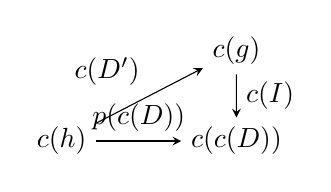
\begin{tikzpicture}[>=stealth,baseline=(current bounding box.center),scale=0.74,
    every node/.style={}]
    \node (Ch) at (0,0) {$c(h)$};
    \node (Cg) at (3.0,1.55) {$c(g)$};
    \node (CcD) at (3.0,0) {$c(c(D))$};
    \draw[->] (Ch) -- node[above left] {$c(D')$} (Cg);
    \draw[->] (Cg) -- node[right] {$c(I)$} (CcD);
    \draw[->] (Ch) -- node[above] {$p(c(D))$} (CcD);
  \end{tikzpicture}
  \tag{3.2.12.1}
\end{equation}
在同伦意义下交换。

\VerdierSemanticAnchor{ch1-3-2-12-c}
c) 图

\VerdierSemanticAnchor{ch1-3-2-12-eq2}
\begin{equation}
  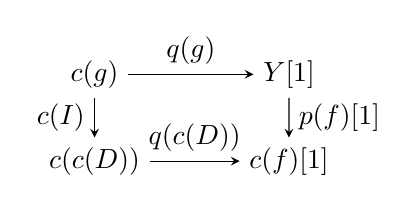
\begin{tikzpicture}[>=stealth,baseline=(current bounding box.center),scale=0.76,
    every node/.style={}]
    \node (Cg) at (0,1.45) {$c(g)$};
    \node (Y) at (3.25,1.45) {$Y[1]$};
    \node (CcD) at (0,0) {$c(c(D))$};
    \node (Cf) at (3.25,0) {$c(f)[1]$};
    \draw[->] (Cg) -- node[above] {$q(g)$} (Y);
    \draw[->] (Cg) -- node[left] {$c(I)$} (CcD);
    \draw[->] (Y) -- node[right] {$p(f)[1]$} (Cf);
    \draw[->] (CcD) -- node[above] {$q(c(D))$} (Cf);
  \end{tikzpicture}
  \tag{3.2.12.2}
\end{equation}
交换。

\VerdierSemanticAnchor{ch1-3-2-12-component-calculation}
事实上，直接计算表明，态射 $c(I)$ 的第 $i$ 个分量为

\VerdierSemanticAnchor{ch1-3-2-12-eq3}
\begin{equation}
  c(I)^i=
  \begin{pmatrix}
    \operatorname{id}&0\\
    0&0\\
    0&\operatorname{id}\\
    0&0
  \end{pmatrix}
  \colon Z^i\oplus Y^{i+1}\longrightarrow
  Z^i\oplus X^{i+1}\oplus Y^{i+1}\oplus X^{i+2}.
  \tag{3.2.12.3}
\end{equation}

\VerdierSemanticAnchor{ch1-3-2-12-inverse}
态射 $u\colon c(c(D))\longrightarrow c(g)$ 的分量为

\VerdierSemanticAnchor{ch1-3-2-12-eq4}
\begin{equation}
  u^i=
  \begin{pmatrix}
    \operatorname{id}&0&0&0\\
    0&f^{i+1}&\operatorname{id}&0
  \end{pmatrix}
  \colon Z^i\oplus X^{i+1}\oplus Y^{i+1}\oplus X^{i+2}
  \longrightarrow Z^i\oplus Y^{i+1}
  \tag{3.2.12.4}
\end{equation}
它在同伦意义下是 $c(I)$ 的逆，从而证明了第一个断言。为证明第二个断言，
只需验证图

\VerdierSemanticAnchor{ch1-3-2-12-eq5}
\begin{equation}
  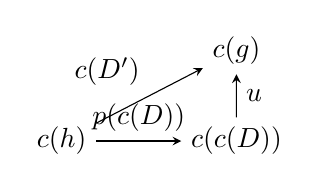
\begin{tikzpicture}[>=stealth,baseline=(current bounding box.center),scale=0.74,
    every node/.style={}]
    \node (Ch) at (0,0) {$c(h)$};
    \node (Cg) at (3.0,1.55) {$c(g)$};
    \node (CcD) at (3.0,0) {$c(c(D))$};
    \draw[->] (Ch) -- node[above left] {$c(D')$} (Cg);
    \draw[->] (CcD) -- node[right] {$u$} (Cg);
    \draw[->] (Ch) -- node[above] {$p(c(D))$} (CcD);
  \end{tikzpicture}
  \tag{3.2.12.5}
\end{equation}

\VerdierSemanticAnchor{ch1-3-2-12-conclusion}
交换；写出各分量即可验证。最后，由 (3.2.2)，态射 $q(f)$ 的函子性质
(3.2.2.2) 蕴含方形 (3.2.12.2) 交换。
\endgroup

\VerdierSourcePageBlock{0095}%
\begingroup
\setlength{\abovedisplayskip}{4pt plus 2pt minus 2pt}%
\setlength{\belowdisplayskip}{4pt plus 2pt minus 2pt}%
\VerdierSemanticAnchor{ch1-3-3}
\subsection{特异三角的性质}

\VerdierSemanticAnchor{ch1-3-3-1}
\noindent\textbf{定义 3.3.1.}\quad
\VerdierSemanticAnchor{ch1-3-3-1-distinguished-triangle}
$K(C)$ 的一个三角
$X\xrightarrow{u}Y\xrightarrow{v}Z\xrightarrow{w}X[1]$ 称为
\emph{特异三角}，如果存在 $\operatorname{Tr}_1(C)$ 的一个对象
$X'\xrightarrow{\dot f'}Y'$ 以及三角的一个同构（(3.2.1.3) 和
(3.2.2.7)）：

\VerdierSemanticAnchor{ch1-3-3-1-isomorphism-diagram}
\begin{center}
  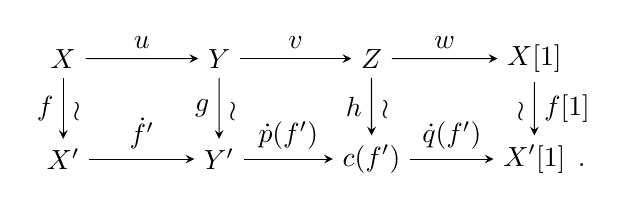
\begin{tikzpicture}[>=stealth,scale=0.88,every node/.style={}]
    \node (X)   at (0,1.45) {$X$};
    \node (Y)   at (2.25,1.45) {$Y$};
    \node (Z)   at (4.45,1.45) {$Z$};
    \node (Xs)  at (6.80,1.45) {$X[1]$};
    \node (Xp)  at (0,0) {$X'$};
    \node (Yp)  at (2.25,0) {$Y'$};
    \node (Cf)  at (4.45,0) {$c(f')$};
    \node (Xps) at (6.80,0) {$X'[1]$};
    \node[anchor=base west,inner sep=0pt,xshift=.08em] at (Xps.base east) {$.$};
    \draw[->] (X) -- node[above] {$u$} (Y);
    \draw[->] (Y) -- node[above] {$v$} (Z);
    \draw[->] (Z) -- node[above] {$w$} (Xs);
    \draw[->] (Xp) -- node[above] {$\dot f'$} (Yp);
    \draw[->] (Yp) -- node[above] {$\dot p(f')$} (Cf);
    \draw[->] (Cf) -- node[above] {$\dot q(f')$} (Xps);
    \draw[->] (X) -- node[left] {$f$} node[right,pos=.55] {$\wr$} (Xp);
    \draw[->] (Y) -- node[left] {$g$} node[right,pos=.55] {$\wr$} (Yp);
    \draw[->] (Z) -- node[left] {$h$} node[right,pos=.55] {$\wr$} (Cf);
    \draw[->] (Xs) -- node[right] {$f[1]$} node[left,pos=.55] {$\wr$} (Xps);
  \end{tikzpicture}
\end{center}

\VerdierSemanticAnchor{ch1-3-3-2}
\noindent\textbf{命题 3.3.2. (TRI)}\quad
\VerdierSemanticAnchor{ch1-3-3-2-isomorphism-invariance}
\textit{$K(C)$ 中任何与一个特异三角同构的三角都是特异三角。}
\VerdierSemanticAnchor{ch1-3-3-2-identity-triangle}
\textit{对于 $K(C)$ 的每个对象 $X$，三角
$X\xrightarrow{\operatorname{id}_X}X\longrightarrow0\longrightarrow X[1]$
是特异三角。}
\VerdierSemanticAnchor{ch1-3-3-2-completion}
\textit{$K(C)$ 的每个态射 $u\colon X\to Y$ 都包含在一个特异三角
$X\xrightarrow{u}Y\xrightarrow{v}Z\xrightarrow{w}X[1]$ 中。}

\VerdierSemanticAnchor{ch1-3-3-2-proof-first}
第一个断言是平凡的。为证明第二个断言，只需证明图

\VerdierSemanticAnchor{ch1-3-3-2-identity-comparison}
\begin{center}
  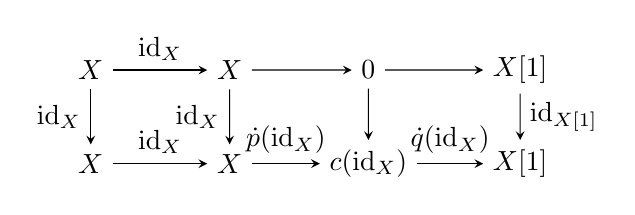
\begin{tikzpicture}[>=stealth,scale=0.82,every node/.style={}]
    \node (X1) at (0,1.45) {$X$};
    \node (X2) at (2.15,1.45) {$X$};
    \node (Z1) at (4.30,1.45) {$0$};
    \node (Xs1) at (6.65,1.45) {$X[1]$};
    \node (X3) at (0,0) {$X$};
    \node (X4) at (2.15,0) {$X$};
    \node (Cid) at (4.30,0) {$c(\operatorname{id}_X)$};
    \node (Xs2) at (6.65,0) {$X[1]$};
    \draw[->] (X1) -- node[above] {$\operatorname{id}_X$} (X2);
    \draw[->] (X2) -- (Z1);
    \draw[->] (Z1) -- (Xs1);
    \draw[->] (X3) -- node[above] {$\operatorname{id}_X$} (X4);
    \draw[->] (X4) -- node[above] {$\dot p(\operatorname{id}_X)$} (Cid);
    \draw[->] (Cid) -- node[above] {$\dot q(\operatorname{id}_X)$} (Xs2);
    \draw[->] (X1) -- node[left] {$\operatorname{id}_X$} (X3);
    \draw[->] (X2) -- node[left] {$\operatorname{id}_X$} (X4);
    \draw[->] (Z1) -- (Cid);
    \draw[->] (Xs1) -- node[right] {$\operatorname{id}_{X[1]}$} (Xs2);
  \end{tikzpicture}
\end{center}

\VerdierSemanticAnchor{ch1-3-3-2-identity-cone-null}
是 $K(C)$ 中三角的一个同构。因此只需证明
$c(\operatorname{id}_X)$ 同伦于零。由 $\operatorname{tr}_1(C)$ 中
同伦的定义 (3.1.4)，立即可知形如

\VerdierSemanticAnchor{ch1-3-3-2-tr1-null-diagram}
\begin{center}
  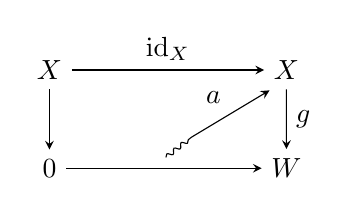
\begin{tikzpicture}[>=stealth,scale=0.86,every node/.style={}]
    \node (X1) at (0,1.45) {$X$};
    \node (X2) at (3.50,1.45) {$X$};
    \node (Z)  at (0,0) {$0$};
    \node (W)  at (3.50,0) {$W$};
    \draw[->] (X1) -- node[above] {$\operatorname{id}_X$} (X2);
    \draw[->] (X1) -- (Z);
    \draw[->] (X2) -- node[right] {$g$} (W);
    \draw[->] (Z) -- (W);
    \draw[decorate,decoration={snake,amplitude=0.8pt,segment length=3.3pt}]
      (1.72,0.16) -- (2.10,0.46);
    \draw[->] (2.10,0.46) -- node[above left] {$a$} (3.25,1.15);
  \end{tikzpicture}
\end{center}

\VerdierSemanticAnchor{ch1-3-3-2-tr1-null-conclusion}
的 $\operatorname{tr}_1(C)$ 的每个态射都同伦于零。
\VerdierSemanticAnchor{ch1-3-3-2-adjunction}
于是锥函子的伴随性质 (3.1.6) 表明
$c(\operatorname{id}_X)$ 同伦于零。
\VerdierSemanticAnchor{ch1-3-3-2-open-morphism}
设 $f\colon X\to Y$ 是一个态射
\endgroup%
\VerdierSourcePageContinue{0096}%
\begingroup
\setlength{\abovedisplayskip}{3pt plus 2pt minus 2pt}%
\setlength{\belowdisplayskip}{3pt plus 2pt minus 2pt}%
\VerdierSemanticAnchor{ch1-3-3-2-open-morphism-continuation}
此态射在 $\operatorname{comp}(C)$ 中属于态射 $u\colon X\to Y$ 的同伦类。
\VerdierSemanticAnchor{ch1-3-3-2-representative}
于是得到 $\operatorname{Tr}_1(C)$ 的一个对象：
$X\xrightarrow{\dot f}Y$。
\VerdierSemanticAnchor{ch1-3-3-2-completion-cone}
特异三角
\begin{equation*}
  X\xrightarrow{u}Y\xrightarrow{\dot p(f)}c(f)
  \xrightarrow{\dot q(f)}X[1]
\end{equation*}
\VerdierSemanticAnchor{ch1-3-3-2-completion-conclusion}
包含态射 $u$。

\VerdierSemanticAnchor{ch1-3-3-3}
\noindent\textbf{命题 3.3.3. (TRII)}\quad
\VerdierSemanticAnchor{ch1-3-3-3-trii}
\textit{$K(C)$ 的三角
$X\xrightarrow{u}Y\xrightarrow{v}Z\xrightarrow{w}X[1]$ 是特异三角，
当且仅当三角
$Y\xrightarrow{v}Z\xrightarrow{w}X[1]\xrightarrow{-u[1]}Y[1]$
是特异三角。}

\VerdierSemanticAnchor{ch1-3-3-3-proof-forward}
设三角 $X\xrightarrow{u}Y\xrightarrow{v}Z\xrightarrow{w}X[1]$
是特异三角。于是它同构于一个如下形式的三角：

\VerdierSemanticAnchor{ch1-3-3-3-cone-model}
\begin{equation*}
  X'\xrightarrow{\dot f}Y'\xrightarrow{\dot p(f)}c(f)
  \xrightarrow{\dot q(f)}X'[1],
\end{equation*}
其中 $X'\xrightarrow{\dot f}Y'$ 是 $\operatorname{Tr}_1(C)$ 的一个对象。
因此只需证明三角

\VerdierSemanticAnchor{ch1-3-3-3-rotated-model}
\begin{equation*}
  Y'\xrightarrow{\dot p(f)}c(f)\xrightarrow{\dot q(f)}X'[1]
  \xrightarrow{-\dot f[1]}Y'[1],
\end{equation*}
是特异三角。由 (3.2.6)，图

\VerdierSemanticAnchor{ch1-3-3-3-comparison}
\begin{center}
  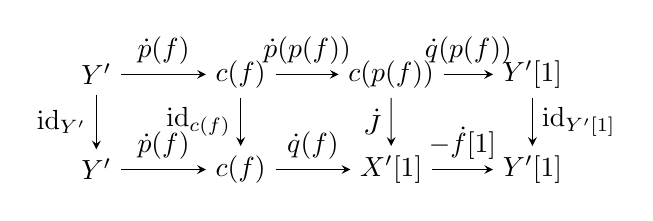
\begin{tikzpicture}[>=stealth,scale=0.78,every node/.style={}]
    \node (Y1)  at (0,1.55) {$Y'$};
    \node (Cf1) at (2.35,1.55) {$c(f)$};
    \node (Cpf) at (4.80,1.55) {$c(p(f))$};
    \node (Ys1) at (7.10,1.55) {$Y'[1]$};
    \node (Y2)  at (0,0) {$Y'$};
    \node (Cf2) at (2.35,0) {$c(f)$};
    \node (Xs)  at (4.80,0) {$X'[1]$};
    \node (Ys2) at (7.10,0) {$Y'[1]$};
    \draw[->] (Y1) -- node[above] {$\dot p(f)$} (Cf1);
    \draw[->] (Cf1) -- node[above] {$\dot p(p(f))$} (Cpf);
    \draw[->] (Cpf) -- node[above] {$\dot q(p(f))$} (Ys1);
    \draw[->] (Y2) -- node[above] {$\dot p(f)$} (Cf2);
    \draw[->] (Cf2) -- node[above] {$\dot q(f)$} (Xs);
    \draw[->] (Xs) -- node[above] {$-\dot f[1]$} (Ys2);
    \draw[->] (Y1) -- node[left] {$\operatorname{id}_{Y'}$} (Y2);
    \draw[->] (Cf1) -- node[left] {$\operatorname{id}_{c(f)}$} (Cf2);
    \draw[->] (Cpf) -- node[left] {$\dot J$} (Xs);
    \draw[->] (Ys1) -- node[right] {$\operatorname{id}_{Y'[1]}$} (Ys2);
  \end{tikzpicture}
\end{center}

\VerdierSemanticAnchor{ch1-3-3-3-forward-conclusion}
是 $K(C)$ 中三角的一个同构。

\VerdierSemanticAnchor{ch1-3-3-3-proof-reverse}
现在设三角
$Y\xrightarrow{v}Z\xrightarrow{w}X[1]\xrightarrow{-u[1]}Y[1]$
是特异三角。由 (3.2.4) 可知三角

\VerdierSemanticAnchor{ch1-3-3-3-shifted-triangle}
\begin{equation*}
  Y[-1]\xrightarrow{v[-1]}Z[-1]\xrightarrow{w[-1]}X
  \xrightarrow{u}Y
\end{equation*}
是特异三角，并且，
\VerdierSemanticAnchor{ch1-3-3-3-double-rotation}
将前述论证应用两次，可知三角
\begin{equation*}
  X\xrightarrow{u}Y\xrightarrow{v}Z\xrightarrow{w}X[1]
\end{equation*}
\VerdierSemanticAnchor{ch1-3-3-3-conclusion}
是特异三角，证明完毕。
\endgroup

\VerdierSourcePageBlock{0097}%
\begingroup
\setlength{\abovedisplayskip}{3pt plus 2pt minus 2pt}%
\setlength{\belowdisplayskip}{3pt plus 2pt minus 2pt}%
\setlength{\jot}{2pt}%
\VerdierSemanticAnchor{ch1-3-3-4}
\noindent\textbf{命题 3.3.4. (TRIII)}\quad
\begingroup\itshape
\VerdierSemanticAnchor{ch1-3-3-4-triii}
设

\VerdierSemanticAnchor{ch1-3-3-4-source-triangles}
\begin{equation*}
  X\xrightarrow{u}Y\xrightarrow{v}Z\xrightarrow{w}X[1],
  \qquad
  X'\xrightarrow{u'}Y'\xrightarrow{v'}Z'\xrightarrow{w'}X'[1]
\end{equation*}
为 $K(C)$ 的两个特异三角，并设

\VerdierSemanticAnchor{ch1-3-3-4-eq1}
\begin{equation}
  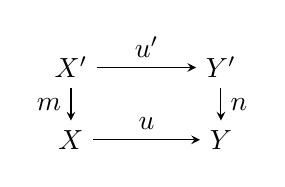
\begin{tikzpicture}[>=stealth,baseline=(current bounding box.center),scale=0.68,
    every node/.style={}]
    \node (Xp) at (0,1.35) {$X'$}; \node (Yp) at (2.8,1.35) {$Y'$};
    \node (X)  at (0,0) {$X$};   \node (Y)  at (2.8,0) {$Y$};
    \draw[->] (Xp) -- node[above] {$u'$} (Yp);
    \draw[->] (Xp) -- node[left] {$m$} (X);
    \draw[->] (Yp) -- node[right] {$n$} (Y);
    \draw[->] (X) -- node[above] {$u$} (Y);
  \end{tikzpicture}
  \tag{3.3.4.1}
\end{equation}
为 $K(C)$ 中的交换方形。
\VerdierSemanticAnchor{ch1-3-3-4-filler}
存在态射 $r\colon Z'\longrightarrow Z$，使得图

\VerdierSemanticAnchor{ch1-3-3-4-morphism-diagram}
\begin{center}
  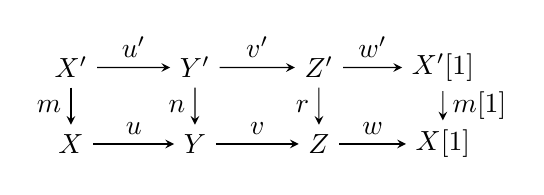
\begin{tikzpicture}[>=stealth,scale=0.67,every node/.style={}]
    \node (Xp)  at (0,1.45) {$X'$};
    \node (Yp)  at (2.35,1.45) {$Y'$};
    \node (Zp)  at (4.70,1.45) {$Z'$};
    \node (Xps) at (7.05,1.45) {$X'[1]$};
    \node (X)   at (0,0) {$X$};
    \node (Y)   at (2.35,0) {$Y$};
    \node (Z)   at (4.70,0) {$Z$};
    \node (Xs)  at (7.05,0) {$X[1]$};
    \draw[->] (Xp) -- node[above] {$u'$} (Yp);
    \draw[->] (Yp) -- node[above] {$v'$} (Zp);
    \draw[->] (Zp) -- node[above] {$w'$} (Xps);
    \draw[->] (X) -- node[above] {$u$} (Y);
    \draw[->] (Y) -- node[above] {$v$} (Z);
    \draw[->] (Z) -- node[above] {$w$} (Xs);
    \draw[->] (Xp) -- node[left] {$m$} (X);
    \draw[->] (Yp) -- node[left] {$n$} (Y);
    \draw[->] (Zp) -- node[left] {$r$} (Z);
    \draw[->] (Xps) -- node[right] {$m[1]$} (Xs);
  \end{tikzpicture}
\end{center}
\VerdierSemanticAnchor{ch1-3-3-4-morphism-conclusion}
是三角的态射。
\endgroup

\VerdierSemanticAnchor{ch1-3-3-4-proof}
按定义，所给三角同构于如下形式的三角：

\VerdierSemanticAnchor{ch1-3-3-4-cone-models}
\begin{align*}
  V&\xrightarrow{\dot f}W\xrightarrow{\dot p(f)}c(f)
     \xrightarrow{\dot q(f)}V[1],\\
  V'&\xrightarrow{\dot f'}W'\xrightarrow{\dot p(f')}c(f')
     \xrightarrow{\dot q(f')}V'[1],
\end{align*}
\VerdierSemanticAnchor{ch1-3-3-4-square-reduction}
因此方形 (3.3.4.1) 同构于方形

\VerdierSemanticAnchor{ch1-3-3-4-homotopy-class-square}
\begin{center}
  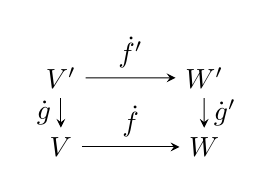
\begin{tikzpicture}[>=stealth,scale=0.65,every node/.style={}]
    \node (Vp) at (0,1.35) {$V'$}; \node (Wp) at (2.8,1.35) {$W'$};
    \node (V)  at (0,0) {$V$};   \node (W)  at (2.8,0) {$W$};
    \draw[->] (Vp) -- node[above] {$\dot f'$} (Wp);
    \draw[->] (Vp) -- node[left] {$\dot g$} (V);
    \draw[->] (Wp) -- node[right] {$\dot g'$} (W);
    \draw[->] (V) -- node[above] {$\dot f$} (W);
  \end{tikzpicture},
\end{center}
\VerdierSemanticAnchor{ch1-3-3-4-representatives}
其中 $g\colon V'\longrightarrow V$ 和 $g'\colon W'\longrightarrow W$
是 $\operatorname{comp}(C)$ 的态射。$\operatorname{comp}(C)$ 中的方形

\VerdierSemanticAnchor{ch1-3-3-4-comp-square}
\begin{center}
  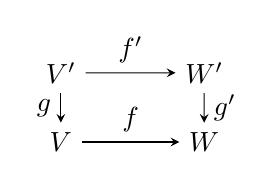
\begin{tikzpicture}[>=stealth,scale=0.65,every node/.style={}]
    \node (Vp) at (0,1.35) {$V'$}; \node (Wp) at (2.8,1.35) {$W'$};
    \node (V)  at (0,0) {$V$};   \node (W)  at (2.8,0) {$W$};
    \draw[->] (Vp) -- node[above] {$f'$} (Wp);
    \draw[->] (Vp) -- node[left] {$g$} (V);
    \draw[->] (Wp) -- node[right] {$g'$} (W);
    \draw[->] (V) -- node[above] {$f$} (W);
  \end{tikzpicture}
\end{center}
\VerdierSemanticAnchor{ch1-3-3-4-open-conclusion}
\endgroup%
\VerdierSourcePageContinue{0098}%
\begingroup
\setlength{\abovedisplayskip}{3pt plus 2pt minus 2pt}%
\setlength{\belowdisplayskip}{3pt plus 2pt minus 2pt}%
\setlength{\jot}{2pt}%
\VerdierSemanticAnchor{ch1-3-3-4-open-conclusion-continuation}
在同伦意义下交换。
\VerdierSemanticAnchor{ch1-3-3-4-homotopy}
取一个同伦 $a\colon fg\rightsquigarrow g'f'$。图

\VerdierSemanticAnchor{ch1-3-3-4-tr1-morphism}
\begin{center}
  $D={}$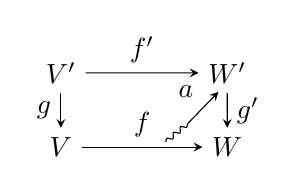
\begin{tikzpicture}[>=stealth,baseline=(current bounding box.center),
    scale=0.65,every node/.style={}]
    \node (Vp) at (0,1.45) {$V'$}; \node (Wp) at (3.25,1.45) {$W'$};
    \node (V)  at (0,0) {$V$};   \node (W)  at (3.25,0) {$W$};
    \draw[->] (Vp) -- node[above] {$f'$} (Wp);
    \draw[->] (Vp) -- node[left] {$g$} (V);
    \draw[->] (Wp) -- node[right] {$g'$} (W);
    \draw[->] (V) -- node[above] {$f$} (W);
    \draw[decorate,decoration={snake,amplitude=0.8pt,segment length=3.3pt}]
      (2.05,0.10) -- (2.48,0.46);
    \draw[->] (2.48,0.46) -- node[above left] {$a$} (3.08,1.08);
  \end{tikzpicture}
\end{center}
是 $\operatorname{tr}_1(C)$ 的态射。由 (3.2.2.7) 可知图

\VerdierSemanticAnchor{ch1-3-3-4-cone-morphism-diagram}
\begin{center}
  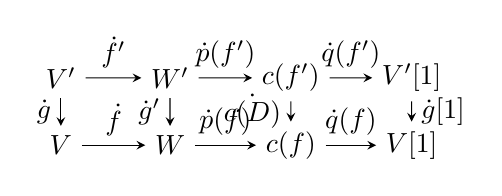
\begin{tikzpicture}[>=stealth,scale=0.59,every node/.style={}]
    \node (Vp)  at (0,1.45) {$V'$};
    \node (Wp)  at (2.35,1.45) {$W'$};
    \node (Cfp) at (4.95,1.45) {$c(f')$};
    \node (Vps) at (7.55,1.45) {$V'[1]$};
    \node (V)   at (0,0) {$V$};
    \node (W)   at (2.35,0) {$W$};
    \node (Cf)  at (4.95,0) {$c(f)$};
    \node (Vs)  at (7.55,0) {$V[1]$};
    \draw[->] (Vp) -- node[above] {$\dot f'$} (Wp);
    \draw[->] (Wp) -- node[above] {$\dot p(f')$} (Cfp);
    \draw[->] (Cfp) -- node[above] {$\dot q(f')$} (Vps);
    \draw[->] (V) -- node[above] {$\dot f$} (W);
    \draw[->] (W) -- node[above] {$\dot p(f)$} (Cf);
    \draw[->] (Cf) -- node[above] {$\dot q(f)$} (Vs);
    \draw[->] (Vp) -- node[left] {$\dot g$} (V);
    \draw[->] (Wp) -- node[left] {$\dot g'$} (W);
    \draw[->] (Cfp) -- node[left] {$\dot{c(D)}$} (Cf);
    \draw[->] (Vps) -- node[right] {$\dot g[1]$} (Vs);
  \end{tikzpicture}
\end{center}
是 $K(C)$ 中三角的态射，从而存在态射

\VerdierSemanticAnchor{ch1-3-3-4-r-conclusion}
\[
  r\colon Z'\longrightarrow Z.
\]

\VerdierSemanticAnchor{ch1-3-3-5}
\noindent\textbf{命题 3.3.5. (TRIV)}\quad
\begingroup\itshape
\VerdierSemanticAnchor{ch1-3-3-5-triv}
设

\VerdierSemanticAnchor{ch1-3-3-5-input-triangle}
\begin{center}
  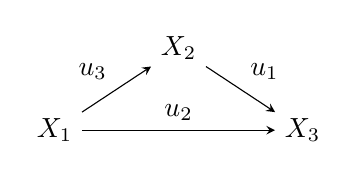
\begin{tikzpicture}[>=stealth,scale=0.67,every node/.style={}]
    \node (X1) at (0,0) {$X_1$};
    \node (X2) at (2.35,1.55) {$X_2$};
    \node (X3) at (4.70,0) {$X_3$};
    \draw[->] (X1) -- node[above left] {$u_3$} (X2);
    \draw[->] (X2) -- node[above right] {$u_1$} (X3);
    \draw[->] (X1) -- node[above] {$u_2$} (X3);
  \end{tikzpicture}
\end{center}
为 $K(C)$ 中的交换图。存在三个特异三角

\VerdierSemanticAnchor{ch1-3-3-5-triangle-3}
\[
  X_1\xrightarrow{u_3}X_2\xrightarrow{v_3}Z_3
  \xrightarrow{w_3}X_1[1],
\]
\VerdierSemanticAnchor{ch1-3-3-5-triangle-1}
\[
  X_2\xrightarrow{u_1}X_3\xrightarrow{v_1}Z_1
  \xrightarrow{w_1}X_2[1],
\]
\VerdierSemanticAnchor{ch1-3-3-5-triangle-2}
\[
  X_1\xrightarrow{u_2}X_3\xrightarrow{v_2}Z_2
  \xrightarrow{w_2}X_1[1]
\]
\VerdierSemanticAnchor{ch1-3-3-5-morphisms}
以及两个态射

\VerdierSemanticAnchor{ch1-3-3-5-m1}
\[
  m_1\colon Z_3\longrightarrow Z_2,
\]
\VerdierSemanticAnchor{ch1-3-3-5-m3}
\[
  m_3\colon Z_2\longrightarrow Z_1,
\]
\VerdierSemanticAnchor{ch1-3-3-5-open-conditions}
使得：
\endgroup
\endgroup%
\VerdierSourcePageContinue{0099}%
\begingroup
\setlength{\abovedisplayskip}{3pt plus 2pt minus 2pt}%
\setlength{\belowdisplayskip}{3pt plus 2pt minus 2pt}%
\setlength{\jot}{2pt}%
\VerdierSemanticAnchor{ch1-3-3-5-condition-a}
\noindent\textit{a) 令图}

\VerdierSemanticAnchor{ch1-3-3-5-morphism-triangles-first}
\begin{center}
  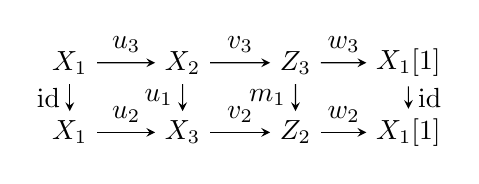
\begin{tikzpicture}[>=stealth,scale=0.61,every node/.style={}]
    \node (X1t) at (0,1.45) {$X_1$};
    \node (X2t) at (2.35,1.45) {$X_2$};
    \node (Z3t) at (4.70,1.45) {$Z_3$};
    \node (X1st) at (7.05,1.45) {$X_1[1]$};
    \node (X1b) at (0,0) {$X_1$};
    \node (X3b) at (2.35,0) {$X_3$};
    \node (Z2b) at (4.70,0) {$Z_2$};
    \node (X1sb) at (7.05,0) {$X_1[1]$};
    \draw[->] (X1t) -- node[above] {$u_3$} (X2t);
    \draw[->] (X2t) -- node[above] {$v_3$} (Z3t);
    \draw[->] (Z3t) -- node[above] {$w_3$} (X1st);
    \draw[->] (X1b) -- node[above] {$u_2$} (X3b);
    \draw[->] (X3b) -- node[above] {$v_2$} (Z2b);
    \draw[->] (Z2b) -- node[above] {$w_2$} (X1sb);
    \draw[->] (X1t) -- node[left] {$\mathrm{id}$} (X1b);
    \draw[->] (X2t) -- node[left] {$u_1$} (X3b);
    \draw[->] (Z3t) -- node[left] {$m_1$} (Z2b);
    \draw[->] (X1st) -- node[right] {$\mathrm{id}$} (X1sb);
  \end{tikzpicture}
\end{center}
\VerdierSemanticAnchor{ch1-3-3-5-morphism-triangles-second}
\begin{center}
  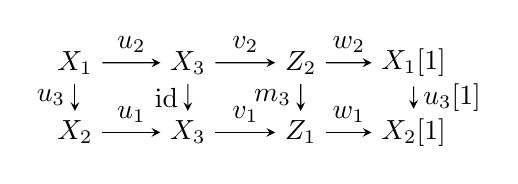
\begin{tikzpicture}[>=stealth,scale=0.61,every node/.style={}]
    \node (X1t) at (0,1.45) {$X_1$};
    \node (X3t) at (2.35,1.45) {$X_3$};
    \node (Z2t) at (4.70,1.45) {$Z_2$};
    \node (X1st) at (7.05,1.45) {$X_1[1]$};
    \node (X2b) at (0,0) {$X_2$};
    \node (X3b) at (2.35,0) {$X_3$};
    \node (Z1b) at (4.70,0) {$Z_1$};
    \node (X2sb) at (7.05,0) {$X_2[1]$};
    \draw[->] (X1t) -- node[above] {$u_2$} (X3t);
    \draw[->] (X3t) -- node[above] {$v_2$} (Z2t);
    \draw[->] (Z2t) -- node[above] {$w_2$} (X1st);
    \draw[->] (X2b) -- node[above] {$u_1$} (X3b);
    \draw[->] (X3b) -- node[above] {$v_1$} (Z1b);
    \draw[->] (Z1b) -- node[above] {$w_1$} (X2sb);
    \draw[->] (X1t) -- node[left] {$u_3$} (X2b);
    \draw[->] (X3t) -- node[left] {$\mathrm{id}$} (X3b);
    \draw[->] (Z2t) -- node[left] {$m_3$} (Z1b);
    \draw[->] (X1st) -- node[right] {$u_3[1]$} (X2sb);
  \end{tikzpicture}
\end{center}
\VerdierSemanticAnchor{ch1-3-3-5-condition-a-conclusion}
\textit{为三角的态射。}

\VerdierSemanticAnchor{ch1-3-3-5-condition-b}
\noindent\textit{b) 令三角}
\VerdierSemanticAnchor{ch1-3-3-5-z-triangle}
\[
  Z_3\xrightarrow{m_1}Z_2\xrightarrow{m_3}Z_1
  \xrightarrow{v_3[1]w_1}Z_3[1]
\]
\VerdierSemanticAnchor{ch1-3-3-5-condition-b-conclusion}
\textit{为特异三角。}

\VerdierSemanticAnchor{ch1-3-3-5-proof}
取 $\operatorname{comp}(C)$ 的态射
$f\colon X_1\longrightarrow X_2$（分别地，
$g\colon X_2\longrightarrow X_3$），使其属于类 $\dot u_3$
（分别地，$\dot u_1$）。
\VerdierSemanticAnchor{ch1-3-3-5-composite}
令 $h=gf\colon X_1\longrightarrow X_3$。态射 $h$ 属于类
$\dot u_2$。为证明该命题，只需取 (3.2.2) 中的三角为特异三角：

\VerdierSemanticAnchor{ch1-3-3-5-cone-triangles}
\begin{align*}
  X_1&\xrightarrow{\dot f}X_2\xrightarrow{\dot p(f)}c(f)
       \xrightarrow{\dot q(f)}X_1[1],\\
  X_2&\xrightarrow{\dot g}X_3\xrightarrow{\dot p(g)}c(g)
       \xrightarrow{\dot q(g)}X_2[1],\\
  X_1&\xrightarrow{\dot h}X_3\xrightarrow{\dot p(h)}c(h)
       \xrightarrow{\dot q(h)}X_1[1]
\end{align*}
\VerdierSemanticAnchor{ch1-3-3-5-cone-morphisms}
并取下列态射为相应的态射：
\[
  c(D)\colon c(f)\longrightarrow c(h),
  \qquad
  c(D')\colon c(h)\longrightarrow c(g),
\]
其中 $D$ 与 $D'$ 是图

\VerdierSemanticAnchor{ch1-3-3-5-d-squares}
\begin{center}
  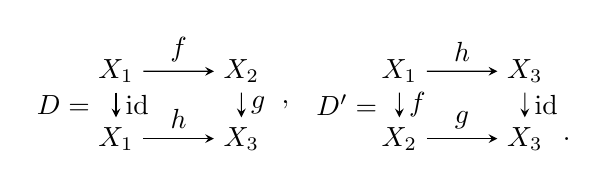
\begin{tikzpicture}[>=stealth,scale=0.59,every node/.style={}]
    \node at (-1.05,0.73) {$D={}$};
    \node (X1t) at (0,1.45) {$X_1$}; \node (X2t) at (2.70,1.45) {$X_2$};
    \node (X1b) at (0,0) {$X_1$};    \node (X3b) at (2.70,0) {$X_3$};
    \draw[->] (X1t) -- node[above] {$f$} (X2t);
    \draw[->] (X1t) -- node[right] {$\mathrm{id}$} (X1b);
    \draw[->] (X2t) -- node[right] {$g$} (X3b);
    \draw[->] (X1b) -- node[above] {$h$} (X3b);
    \node at (3.65,0.73) {$,$};
    \node at (5.05,0.73) {$D'={}$};
    \node (Y1t) at (6.10,1.45) {$X_1$}; \node (Y3t) at (8.80,1.45) {$X_3$};
    \node (Y2b) at (6.10,0) {$X_2$};    \node (Y3b) at (8.80,0) {$X_3$};
    \draw[->] (Y1t) -- node[above] {$h$} (Y3t);
    \draw[->] (Y1t) -- node[right] {$f$} (Y2b);
    \draw[->] (Y3t) -- node[right] {$\mathrm{id}$} (Y3b);
    \draw[->] (Y2b) -- node[above] {$g$} (Y3b);
    \node at (9.70,0.00) {$.$};
  \end{tikzpicture}
\end{center}
\endgroup

\VerdierSourcePageBlock{0100}%
\begingroup
\VerdierSemanticAnchor{ch1-3-3-5-proof-completion}
事实上，第一项断言是 (3.2.2) 的直接推论；由命题 (3.2.12)，存在态射
$c(I)\colon c(g)\longrightarrow c(c(D))$，使得下图

\VerdierSemanticAnchor{ch1-3-3-5-isomorphism-diagram}
\begin{center}
  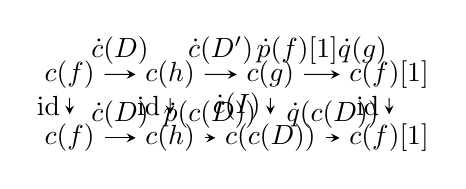
\begin{tikzpicture}[>=stealth,scale=0.52,every node/.style={}]
    \node (cf1) at (0,1.55) {$c(f)$};
    \node (ch1) at (2.45,1.55) {$c(h)$};
    \node (cg1) at (4.90,1.55) {$c(g)$};
    \node (cfs1) at (7.80,1.55) {$c(f)[1]$};
    \node (cf2) at (0,0) {$c(f)$};
    \node (ch2) at (2.45,0) {$c(h)$};
    \node (ccd) at (4.90,0) {$c(c(D))$};
    \node (cfs2) at (7.80,0) {$c(f)[1]$};
    \draw[->] (cf1) -- node[above] {$\dot c(D)$} (ch1);
    \draw[->] (ch1) -- node[above] {$\dot c(D')$} (cg1);
    \draw[->] (cg1) -- node[above] {$\dot p(f)[1]\dot q(g)$} (cfs1);
    \draw[->] (cf2) -- node[above] {$\dot c(D)$} (ch2);
    \draw[->] (ch2) -- node[above] {$\dot p(c(D))$} (ccd);
    \draw[->] (ccd) -- node[above] {$\dot q(c(D))$} (cfs2);
    \draw[->] (cf1) -- node[left] {$\mathrm{id}$} (cf2);
    \draw[->] (ch1) -- node[left] {$\mathrm{id}$} (ch2);
    \draw[->] (cg1) -- node[left] {$\dot c(I)$} (ccd);
    \draw[->] (cfs1) -- node[left] {$\mathrm{id}$} (cfs2);
  \end{tikzpicture}
\end{center}
\VerdierSemanticAnchor{ch1-3-3-5-proof-complete}
是三角的同构。

\VerdierSemanticAnchor{ch1-3-3-6}
\noindent\textbf{3.3.6.} 设
$F\colon \mathcal{J}\longrightarrow\operatorname{comp}(C)$ 为函子。以
$\mathcal{F}\ell_n(\mathcal{J})$ 表示 $\mathcal{J}$ 中由 $n$ 个可复合态射组成的
序列所构成的范畴：$\mathcal{F}\ell_n(\mathcal{J})$ 的对象是 $\mathcal{J}$ 中的图式

\VerdierSemanticAnchor{ch1-3-3-6-object-diagram}
\[
  i_1\xrightarrow{f_1}i_2\xrightarrow{f_2}i_3
  \longrightarrow\cdots\xrightarrow{f_n}i_{n+1}.
\]
\VerdierSemanticAnchor{ch1-3-3-6-morphism}
设 $(i_p,f_p)$ 和 $(j_p,g_p)$ 是 $\mathcal{J}$ 中两个由 $n$ 个可复合态射组成的
序列。$\mathcal{F}\ell_n(\mathcal{J})$ 中从 $(i_p,f_p)$ 到 $(j_p,g_p)$ 的一个
态射是交换图式

\VerdierSemanticAnchor{ch1-3-3-6-morphism-diagram}
\begin{center}
  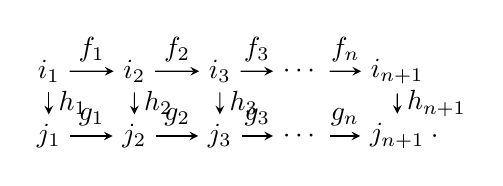
\begin{tikzpicture}[>=stealth,scale=0.53,every node/.style={}]
    \node (i1) at (0,1.55) {$i_1$};
    \node (i2) at (2.05,1.55) {$i_2$};
    \node (i3) at (4.10,1.55) {$i_3$};
    \node (idots) at (6.05,1.55) {$\cdots$};
    \node (in) at (8.35,1.55) {$i_{n+1}$};
    \node (j1) at (0,0) {$j_1$};
    \node (j2) at (2.05,0) {$j_2$};
    \node (j3) at (4.10,0) {$j_3$};
    \node (jdots) at (6.05,0) {$\cdots$};
    \node (jn) at (8.35,0) {$j_{n+1}$};
    \draw[->] (i1) -- node[above] {$f_1$} (i2);
    \draw[->] (i2) -- node[above] {$f_2$} (i3);
    \draw[->] (i3) -- node[above] {$f_3$} (idots);
    \draw[->] (idots) -- node[above] {$f_n$} (in);
    \draw[->] (j1) -- node[above] {$g_1$} (j2);
    \draw[->] (j2) -- node[above] {$g_2$} (j3);
    \draw[->] (j3) -- node[above] {$g_3$} (jdots);
    \draw[->] (jdots) -- node[above] {$g_n$} (jn);
    \draw[->] (i1) -- node[right] {$h_1$} (j1);
    \draw[->] (i2) -- node[right] {$h_2$} (j2);
    \draw[->] (i3) -- node[right] {$h_3$} (j3);
    \draw[->] (in) -- node[right] {$h_{n+1}$} (jn);
    \node at (9.25,0) {$.$};
  \end{tikzpicture}
\end{center}
\VerdierSemanticAnchor{ch1-3-3-6-composition}
态射的复合以显然的方式定义。以 $\mathrm{Fl}_n(\mathcal{J})$ 表示
$\mathcal{F}\ell_n(\mathcal{J})$ 的对象集。

\VerdierSemanticAnchor{ch1-3-3-6-cone-functor}
设 $i\xrightarrow{f}j$ 是 $\mathcal{F}\ell_1(\mathcal{J})$ 的对象。应用函子 $F$
得到 $\operatorname{comp}(C)$ 中的态射
\[
  F(i)\xrightarrow{F(f)}F(j),
\]
它可视为 $\operatorname{Tr}_1(C)$ 的对象；于是应用映射锥函子得到函子
$S\colon\mathcal{F}\ell_1(\mathcal{J})\longrightarrow\mathrm{K}(C)$：

\VerdierSemanticAnchor{ch1-3-3-6-1}
\begin{equation}
  S(f)=S\bigl(i\xrightarrow{f}j\bigr)
  =c\bigl(F(i)\xrightarrow{F(f)}F(j)\bigr).
  \tag{3.3.6.1}
\end{equation}
\endgroup

\VerdierSourcePageBlock{0101}%
\begingroup
\VerdierSemanticAnchor{ch1-3-3-6-two-arrow-object}
现在设 $i\xrightarrow{f}j\xrightarrow{g}k$ 是
$\mathcal{F}\ell_2(\mathcal{J})$ 的对象。将其对应于 $\operatorname{Tr}_1(C)$ 中的
下图：

\VerdierSemanticAnchor{ch1-3-3-6-2}
\begin{equation}
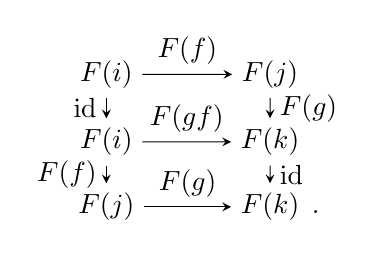
\begin{tikzpicture}[>=stealth,baseline=(current bounding box.center),scale=0.66,
  every node/.style={}]
  \node (Fi1) at (0,2.55) {$F(i)$};
  \node (Fj1) at (3.15,2.55) {$F(j)$};
  \node (Fi2) at (0,1.25) {$F(i)$};
  \node (Fk1) at (3.15,1.25) {$F(k)$};
  \node (Fj2) at (0,0) {$F(j)$};
  \node (Fk2) at (3.15,0) {$F(k)$};
  \draw[->] (Fi1) -- node[above] {$F(f)$} (Fj1);
  \draw[->] (Fi2) -- node[above] {$F(gf)$} (Fk1);
  \draw[->] (Fj2) -- node[above] {$F(g)$} (Fk2);
  \draw[->] (Fi1) -- node[left] {$\mathrm{id}$} (Fi2);
  \draw[->] (Fj1) -- node[right] {$F(g)$} (Fk1);
  \draw[->] (Fi2) -- node[left] {$F(f)$} (Fj2);
  \draw[->] (Fk1) -- node[right] {$\mathrm{id}$} (Fk2);
  \node[anchor=base west,inner sep=0pt,xshift=.08em] at (Fk2.base east) {$.$};
\end{tikzpicture}
\tag{3.3.6.2}
\end{equation}

\VerdierSemanticAnchor{ch1-3-3-6-delta}
定义
\begin{equation}
\begin{aligned}
  \delta(f,g)&\colon S(g)\longrightarrow S(f)[1],\\
  \delta(f,g)&=\dot p(F(f))[1]\dot q(F(g)).
\end{aligned}
\tag{3.3.6.3}
\end{equation}
对图 (3.3.6.2) 应用映射锥函子，得到从
$\mathcal{F}\ell_2(\mathcal{J})$ 到 $K(C)$ 中三角范畴的函子：

\VerdierSemanticAnchor{ch1-3-3-6-4}
\begin{equation}
  \bigl(i\xrightarrow{f}j\xrightarrow{g}k\bigr)
  \longmapsto
  S(f)\longrightarrow S(gf)\longrightarrow S(g)
  \xrightarrow{\delta(f,g)}S(f)[1].
  \tag{3.3.6.4}
\end{equation}
\VerdierSemanticAnchor{ch1-3-3-6-distinguished-conclusion}
(3.3.5) 证明的末尾表明三角
\[
  S(f)\longrightarrow S(gf)\longrightarrow S(g)
  \xrightarrow{\delta(f,g)}S(f)[1]
\]
是特异三角。

\VerdierSemanticAnchor{ch1-3-4}
\subsection{特异三角的函子性质}

\VerdierSemanticAnchor{ch1-3-4-1}
\noindent\textbf{命题 3.4.1.}\quad
设 $\iota_1\colon K(C)^{\circ}\longrightarrow K(C^{\circ})$ 是典范同构
(2.5.13)，并设
\[
  X\xrightarrow{u}Y\xrightarrow{v}Z\xrightarrow{w}X[1]
\]
是 $K(C)$ 中的特异三角。则 $K(C^{\circ})$ 中的三角
\VerdierSemanticAnchor{ch1-3-4-1-opposite-triangle}
\[
  (\iota_1X)[-1]\xrightarrow{\iota_1w}\iota_1Z
  \xrightarrow{\iota_1v}\iota_1Y
  \xrightarrow{-\iota_1u}\iota_1X
\]
是特异三角。
\endgroup

\VerdierSourcePageBlock{0102}%
\begingroup
\VerdierSemanticAnchor{ch1-3-4-1-proof}
由 (3.3.1)，总可以假定所给三角具有如下形式：

\VerdierSemanticAnchor{ch1-3-4-1-cone-model}
\[
  X\xrightarrow{\dot f}Y\xrightarrow{\dot p(f)}c(f)
  \xrightarrow{\dot q(f)}X[1]
\]
其中 $f\colon X\longrightarrow Y$ 是 $\operatorname{comp}(C)$ 中的态射。
只需证明三角

\VerdierSemanticAnchor{ch1-3-4-1-goal-triangle}
\[
  (\iota_1X)[-1]\xrightarrow{\iota_1\dot q(f)}\iota_1c(f)
  \xrightarrow{\iota_1\dot p(f)}\iota_1Y
  \xrightarrow{-(\iota_1\dot f)}\iota_1X
\]
是特异三角（$\iota_1f$ 是态射 $f$ 在
$\iota_1\colon\operatorname{comp}(C)^{\circ}\longrightarrow
\operatorname{comp}(C^{\circ})$ 下的像）。由 $\iota_1$ 的定义 (2.4.1) 以及
映射锥函子的定义 (3.1.2)，立即可知复形 $\iota_1c(f)$ 的分量和微分为

\VerdierSemanticAnchor{ch1-3-4-1-components}
\[
  \iota_1c(f)^i=(\iota_1X)^{i-1}\oplus(\iota_1Y)^i,
\]
\VerdierSemanticAnchor{ch1-3-4-1-1}
\begin{equation}
  d_{\iota_1c(f)}^i=
  \begin{pmatrix}
    -d_{\iota_1X}^{i-1} & (\iota_1f)^i\\
    0 & d_{\iota_1Y}^{i}
  \end{pmatrix}.
  \tag{3.4.1.1}
\end{equation}
\VerdierSemanticAnchor{ch1-3-4-1-cone-identity}
因此
\[
  \iota_1c(f)=c(-\iota_1f)[-1],
\]
并且可验证下图交换：

\VerdierSemanticAnchor{ch1-3-4-1-comparison}
\begin{center}
  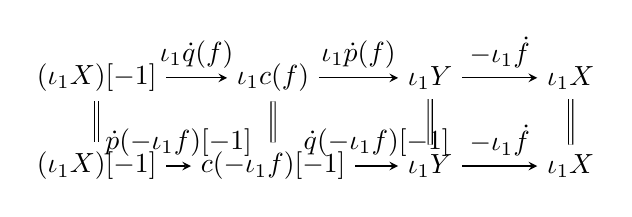
\begin{tikzpicture}[>=stealth,scale=0.70,every node/.style={}]
    \node (x1) at (0,1.60) {$(\iota_1X)[-1]$};
    \node (c1) at (3.20,1.60) {$\iota_1c(f)$};
    \node (y1) at (6.05,1.60) {$\iota_1Y$};
    \node (z1) at (8.60,1.60) {$\iota_1X$};
    \node (x2) at (0,0) {$(\iota_1X)[-1]$};
    \node (c2) at (3.20,0) {$c(-\iota_1f)[-1]$};
    \node (y2) at (6.05,0) {$\iota_1Y$};
    \node (z2) at (8.60,0) {$\iota_1X$};
    \draw[->] (x1) -- node[above] {$\iota_1\dot q(f)$} (c1);
    \draw[->] (c1) -- node[above] {$\iota_1\dot p(f)$} (y1);
    \draw[->] (y1) -- node[above] {$-\iota_1\dot f$} (z1);
    \draw[->] (x2) -- node[above] {$\dot p(-\iota_1f)[-1]$} (c2);
    \draw[->] (c2) -- node[above] {$\dot q(-\iota_1f)[-1]$} (y2);
    \draw[->] (y2) -- node[above] {$-\iota_1\dot f$} (z2);
    \draw[double,double distance=1.1pt] (x1) -- (x2);
    \draw[double,double distance=1.1pt] (c1) -- (c2);
    \draw[double,double distance=1.1pt] (y1) -- (y2);
    \draw[double,double distance=1.1pt] (z1) -- (z2);
  \end{tikzpicture}
\end{center}
\VerdierSemanticAnchor{ch1-3-4-1-proof-complete}
于是应用 (3.3.3) 即完成证明。

\VerdierSemanticAnchor{ch1-3-4-2}
\noindent\textbf{3.4.2.}\quad
\VerdierSemanticAnchor{ch1-3-4-2-multiadditive-functor}
设 $F\colon\prod_{i\in[n]}C_i\longrightarrow C$ 为多加法函子。为具体起见，
假定 $C$ 中可数乘积可表示。设
\[
  K_{\Pi}F\colon\prod_{i\in[n]}K(C_i)\longrightarrow K(C)
\]
\VerdierSemanticAnchor{ch1-3-4-2-homotopy-extension}
为 $F$ 在复形同伦范畴上的 $\Pi$-扩张，并设

\VerdierSemanticAnchor{ch1-3-4-2-shift-isomorphisms}
\[
  p_i\colon K_{\Pi}F(X_1,\ldots,X_i[1],\ldots,X_n)
  \longrightarrow K_{\Pi}F(X_1,\ldots,X_i,\ldots,X_n)[1]
\]
为典范函子同构。
\endgroup

\VerdierSourcePageBlock{0103}%
\begingroup
\VerdierSemanticAnchor{ch1-3-4-2-variable-specialization}
设 $j\in[n]$，并对每个 $i\neq j$ 设 $X_i$ 为 $K(C_i)$ 的对象。以
\[
  G\colon K(C_j)\longrightarrow K(C)
\]
表示函子

\VerdierSemanticAnchor{ch1-3-4-2-1}
\begingroup
\makeatletter
\tagsleft@true
\let\veqno\@@leqno
\makeatother
\begin{equation}
  X\longmapsto G(X)=K_{\Pi}F(X_1,\ldots,X,\ldots,X_n),
  \tag{3.4.2.1}
\end{equation}
\endgroup
\VerdierSemanticAnchor{ch1-3-4-2-translation-isomorphism}
并以
\[
  m\colon G(X[1])\xrightarrow{\sim}G(X)[1]
\]
表示由 $p_j$ 导出的函子同构。

\VerdierSemanticAnchor{ch1-3-4-3}
\noindent\textbf{命题 3.4.3.}\quad
\emph{设 $K(C_j)$ 中任一特异三角为}
\VerdierSemanticAnchor{ch1-3-4-3-input-triangle}
\[
  X\xrightarrow{u}Y\xrightarrow{v}Z\xrightarrow{w}X[1]
\]
\emph{则 $K(C)$ 中的三角}
\VerdierSemanticAnchor{ch1-3-4-3-image-triangle}
\[
  G(X)\xrightarrow{G(u)}G(Y)\xrightarrow{G(v)}G(Z)
  \xrightarrow{mG(w)}G(X)[1]
\]
\emph{是特异三角。}

\VerdierSemanticAnchor{ch1-3-4-3-proof}
首先可以假定 $K(C_j)$ 中的特异三角具有 (3.3.1) 的形式：
\VerdierSemanticAnchor{ch1-3-4-3-cone-model}
\[
  X\xrightarrow{\dot f}Y\xrightarrow{\dot p(f)}c(f)
  \xrightarrow{\dot q(f)}X[1],
\]
其中 $f\colon X\longrightarrow Y$ 是 $\operatorname{comp}(C_j)$ 中的态射。
以
\VerdierSemanticAnchor{ch1-3-4-3-complex-functor}
\[
  H\colon\operatorname{comp}(C_j)\longrightarrow\operatorname{comp}(C)
\]
表示函子
\[
  X\longmapsto H(X)=\operatorname{comp}_{\Pi}F
  (X_1,\ldots,X,\ldots,X_n),
\]
\VerdierSemanticAnchor{ch1-3-4-3-complex-translation-isomorphism}
并以
\[
  m\colon H(X[1])\xrightarrow{\sim}H(X)[1]
\]
表示在方向 $j$ 上与平移交换的函子同构。函子 $(G,m)$ 是由函子 $(H,m)$
传至复形同伦范畴而得。为证明命题，只需证明
$\operatorname{comp}(C)$ 中存在复形同构

\VerdierSemanticAnchor{ch1-3-4-3-cone-isomorphism}
\[
  J\colon H(c(f))\xrightarrow{\sim}c(H(f))
\]
使下图交换：

\VerdierSemanticAnchor{ch1-3-4-3-1}
\begin{equation}
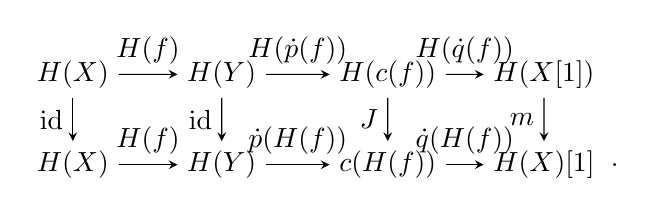
\begin{tikzpicture}[>=stealth,scale=0.62,every node/.style={}]
  \node (x1) at (0,1.85) {$H(X)$};
  \node (y1) at (3.05,1.85) {$H(Y)$};
  \node (c1) at (6.45,1.85) {$H(c(f))$};
  \node (s1) at (9.65,1.85) {$H(X[1])$};
  \node (x2) at (0,0) {$H(X)$};
  \node (y2) at (3.05,0) {$H(Y)$};
  \node (c2) at (6.45,0) {$c(H(f))$};
  \node (s2) at (9.65,0) {$H(X)[1]$};
  \draw[->] (x1) -- node[above] {$H(f)$} (y1);
  \draw[->] (y1) -- node[above] {$H(\dot p(f))$} (c1);
  \draw[->] (c1) -- node[above] {$H(\dot q(f))$} (s1);
  \draw[->] (x2) -- node[above] {$H(f)$} (y2);
  \draw[->] (y2) -- node[above] {$\dot p(H(f))$} (c2);
  \draw[->] (c2) -- node[above] {$\dot q(H(f))$} (s2);
  \draw[->] (x1) -- node[left] {$\mathrm{id}$} (x2);
  \draw[->] (y1) -- node[left] {$\mathrm{id}$} (y2);
  \draw[->] (c1) -- node[left] {$J$} (c2);
  \draw[->] (s1) -- node[left] {$m$} (s2);
  \node[anchor=west,inner sep=0pt] at ([xshift=0.35em]s2.east) {$.$};
\end{tikzpicture}
\tag{3.4.3.1}
\end{equation}
\endgroup

\VerdierSourcePageBlock{0104}%
\begingroup
\VerdierSemanticAnchor{ch1-3-4-3-zero-differential-complex}
对每个复形 $X$，以 $\overline{X}$ 表示保留 $X$ 的各分量而将微分置零所得的
复形。由 $H$ 的定义立即可得
$\overline{H(X)}=H(\overline{X})$。同样，对每个复形态射
$f\colon X\longrightarrow Y$，以
$\overline{f}\colon\overline{X}\longrightarrow\overline{Y}$ 表示保留 $f$ 的各分量
所得的态射。由映射锥函子的定义可知
$c(\overline{f})=\overline{Y}\oplus\overline{X[1]}$，且
$p(\overline{f})\colon\overline{Y}\longrightarrow c(\overline{f})$ 是第一分量的
典范包含态射，
$q(\overline{f})\colon c(\overline{f})\longrightarrow\overline{X[1]}$ 是到第二分量
的典范投影。

\VerdierSemanticAnchor{ch1-3-4-3-cone-graded-splitting}
由于函子 $H$ 和函子“$\overline{\phantom{X}}$”均为加性函子，故
$\overline{H(c(f))}=\overline{H(Y)}\oplus\overline{H(X[1])}$，且
$\overline{H(p(f))}\colon\overline{H(Y)}\longrightarrow\overline{H(c(f))}$ 是第一
分量的典范包含态射，
$\overline{H(q(f))}\colon\overline{H(c(f))}\longrightarrow\overline{H(X[1])}$ 是到
第二分量的典范投影。因此
\[
  H(c(f))^l=H(Y)^l\oplus H(X[1])^l,
\]

\VerdierSemanticAnchor{ch1-3-4-3-2}
\begin{equation}
  d_{H(c(f))}^{,l}=
  \begin{pmatrix}
    d_{H(Y)}^{,l} & \Phi^l\\
    0 & d_{H(X[1])}^{,l}
  \end{pmatrix},
  \tag{3.4.3.2}
\end{equation}

\VerdierSemanticAnchor{ch1-3-4-3-phi-map}
\[
  \Phi^l\colon H(X[1])^l\longrightarrow H(Y)^{l+1}.
\]
$H(c(f))$ 的微分写成这一形式，只是表达 $H(p(f))$ 和 $H(q(f))$ 是复形态射。
为计算 $\Phi^l$，须回到函子 $H$ 的定义，从而回到关联单复形函子的定义
(2.2.2.5)。有

\VerdierSemanticAnchor{ch1-3-4-3-x-shift-components}
\[
  H(X[1])^l=
  \prod_{\substack{\sigma=\sum_i l_i e_i\\ \sum_i l_i=l}}
  F(X_1^{l_1},\ldots,X^{l_j+1},\ldots,X_n^{l_n}),
\]

\VerdierSemanticAnchor{ch1-3-4-3-3}
\begin{equation}
  H(Y)^{l+1}=
  \prod_{\substack{\sigma=\sum_i l_i e_i\\ \sum_i l_i=l}}
  F(X_1^{l_1},\ldots,Y^{l_j+1},\ldots,X_n^{l_n}),
  \tag{3.4.3.3}
\end{equation}

\VerdierSemanticAnchor{ch1-3-4-3-phi-components}
\[
  \Phi^l=
  \prod_{\substack{\sigma=\sum_i l_i e_i\\ \sum_i l_i=l}}
  \varepsilon(\sigma,j)
  F(X_1^{l_1},\ldots,f^{l_j+1},\ldots,X_n^{l_n}).
\]
\endgroup

\VerdierSourcePageBlock{0105}%
\begingroup
\VerdierSemanticAnchor{ch1-3-4-3-cone-of-hf}
另一方面，由映射锥函子的定义可得
\[
  c(H(f))^l=H(Y)^l\oplus(H(X)[1])^l,
\]

\VerdierSemanticAnchor{ch1-3-4-3-4}
\begin{equation}
  d_{c(H(f))}^{,l}=
  \begin{pmatrix}
    d_{H(Y)}^{,l} & H(f)^{l+1}\\
    0 & d_{H(X)[1]}^{,l}
  \end{pmatrix},
  \tag{3.4.3.4}
\end{equation}
其中态射 $H(f)$ 由 (2.4.2.6)、(2.4.2.3) 和 (2.2.2.6) 定义：

\VerdierSemanticAnchor{ch1-3-4-3-5}
\begin{equation}
  H(f)^{l+1}=
  \prod_{\substack{\sigma=\sum_i l_i e_i\\ \sum_i l_i=l}}
  F(X_1^{l_1},\ldots,f^{l_j+1},\ldots,X_n^{l_n}).
  \tag{3.4.3.5}
\end{equation}

\VerdierSemanticAnchor{ch1-3-4-3-j-map}
现定义
\[
  J^l\colon H(Y)^l\oplus H(X[1])^l
  \longrightarrow H(Y)^l\oplus(H(X)[1])^l,
\]

\VerdierSemanticAnchor{ch1-3-4-3-6}
\begin{equation}
  J^l=
  \begin{pmatrix}
    \operatorname{id}_{H(Y)^l} & 0\\
    0 & \Psi^l
  \end{pmatrix},
  \qquad
  \Psi^l=
  \prod_{\substack{\sigma=\sum_i l_i e_i\\ \sum_i l_i=l}}
  \varepsilon(\sigma,j)
  \operatorname{id}_{F(X_1^{l_1},\ldots,X^{l_j+1},\ldots,X_n^{l_n})}.
  \tag{3.4.3.6}
\end{equation}

\VerdierSemanticAnchor{ch1-3-4-3-7}
为验证各 $J^l$ 是一个复形态射的分量，只需验证
\begin{equation}
  \Phi^l=H(f)^{l+1}\Psi^l,
  \qquad
  \Psi^{l+1}d_{H(X[1])}^{l}=d_{H(X)[1]}^{l}\Psi^l.
  \tag{3.4.3.7}
\end{equation}

\VerdierSemanticAnchor{ch1-3-4-3-8}
为验证图 (3.4.3.1) 交换，只需验证
\begin{equation}
  \Psi^l=m^l.
  \tag{3.4.3.8}
\end{equation}
\endgroup

\VerdierSourcePageBlock{0106}%
\begingroup


\VerdierSemanticAnchor{ch1-3-4-3-verification}
(3.4.3.7) 中的第一个等式是显然的（(3.4.3.3) 与 (3.4.3.5)）。
(3.4.3.7) 中的第二个等式由 (3.4.3.8) 得出。为验证 (3.4.3.8)，
只需参照态射 $m$ 的定义 (2.3.2.1)。

\VerdierSemanticAnchor{ch1-3-4-4}
\noindent\textbf{3.4.4.}\quad
当 $C$ 中可数直和可表示时，对函子 $K_{\Sigma}F$ 有一个与命题 (3.4.3)
类似的命题。其证明只需在命题 (3.4.3) 的证明中以直和代替乘积。
\endgroup

\VerdierSourcePageSilent{0107}%

\clearpage
\VerdierSourcePageBlock{0108}%
\begingroup
\VerdierSemanticAnchor{ch1-app-signs}
\section*{附录：关于符号选择的说明}
\addcontentsline{toc}{section}{附录：关于符号选择的说明}

\VerdierSemanticAnchor{ch1-app-signs-cone}
映射锥函子由其伴随性质 (3.1.3) 在唯一同构的意义下所确定。为了便于把
$\operatorname{tr}_1(C)$ 的一个态射关联到 $\operatorname{comp}(C)$ 的一个三角，
我们选择“态射 $X\longrightarrow 0$ 的映射锥”作为平移函子（(3.1.7) 和
(3.2.2.7)），也就是说，平移次数并改变微分的符号。

\VerdierSemanticAnchor{ch1-app-signs-strict}
设 $F\colon\prod_{i\in[n]}C_i\longrightarrow C$ 是一个多加法函子。范畴
$\prod_{i\in[n]}\operatorname{comp}(C_i)$ 自然带有一个 $\mathbb Z[n]$-范畴结构。
如果要求函子
\[
  F^{[n]}\colon\prod_{i\in[n]}\operatorname{comp}(C_i)
  \longrightarrow\operatorname{comp}^{n}(C)
\]
是一个严格 $\mathbb Z[n]$-函子，就会得到我们所采用的平移约定：沿一个方向
平移次数，并改变相应微分的符号。

\VerdierSemanticAnchor{ch1-app-signs-simple-complex}
关于关联单复形函子的选择，我们采用了 [1] 的约定（但在我们的多重复形中，
各微分彼此交换）。这使得可以定义函子
$K_{\Pi}F\colon\prod_i K(C_i)\longrightarrow K(C)$。此时
$K_{\Pi}F(X_1,\ldots,X_i[1],\ldots,X_n)$ 与
$K_{\Pi}F(X_1,\ldots,X_i,\ldots,X_n)[1]$ 不同。为了仍能断言函子
$K_{\Pi}F$ 把特异三角送到特异三角，我们必须定义同构

\VerdierSemanticAnchor{ch1-app-signs-shift-isomorphism}
\[
  p_i\colon K_{\Pi}F(X_1,\ldots,X_i[1],\ldots,X_n)
  \xrightarrow{\ \sim\ }
  K_{\Pi}F(X_1,\ldots,X_i,\ldots,X_n)[1]
\]
（见 (3.4.3) 的证明）。

\VerdierSemanticAnchor{ch1-app-signs-anticommutativity}
于是，当 $i\ne j$ 时，得到反交换图：

\VerdierSemanticAnchor{ch1-app-signs-diagram}
\begin{center}
  \mbox{%
    $\begin{tikzcd}[ampersand replacement=\&,column sep=3.2em,row sep=4.3em]
      K_{\Pi}F(X_1,\ldots,X_i[1],\ldots,X_j[1],\ldots)
        \arrow[r,"p_j"]
        \arrow[d,"p_i"']
        \& K_{\Pi}F(X_1,\ldots,X_i[1],\ldots,X_j,\ldots)[1]
          \arrow[d,"p_i"] \\
      K_{\Pi}F(X_1,\ldots,X_i,\ldots,X_j[1],\ldots)[1]
        \arrow[r,"p_j"]
        \& K_{\Pi}F(X_1,\ldots,X_i,\ldots,X_j,\ldots)[2].
    \end{tikzcd}$%
  }
\end{center}

\VerdierSemanticAnchor{ch1-app-signs-koszul-choice}
随后我们在 (1.5.2) 中说明了如何把这些同构相容地扩张为同构 $p(\sigma)$，
它对每个 $\sigma\in\mathbb Z[n]$ 都有定义。这里包含一个任意选择：需要在
一个本身已确定的上同调类，即 Koszul 类 (1.6.3) 中选择一个余循环。为了符合
通常接受的规则（例如 [1]），我们在所有情形下都选择 Koszul 余循环 (1.6.6)。
\endgroup

\VerdierSourcePageSilent{0109}%

\clearpage
\chapter{三角范畴}
\VerdierSourcePageBlock{0110}%
\VerdierSemanticAnchor{ch2}
\begingroup
\VerdierSemanticAnchor{ch2-1}
\section{定义与初步性质}

\VerdierSemanticAnchor{ch2-1-1}
\subsection{三角范畴的定义}

\VerdierSemanticAnchor{ch2-1-1-1}
\noindent\textbf{定义 1.1.1.}\quad
一个\emph{三角范畴} $\mathcal D$ 是一个严格加法 $\mathbb Z$-范畴
（第一章，1.5.11），并配有一族三角（第一章，3.2.1），称为\emph{特异三角}，
它们具有下列性质：

\VerdierSemanticAnchor{ch2-1-1-1-tri}
\smallskip
\noindent\textbf{TRI:}
$\mathcal D$ 中任何与一个特异三角同构的三角都是特异三角。对于每个对象
$X$（属于 $\mathcal D$），三角
\[
  X\xrightarrow{\operatorname{id}_X}X\longrightarrow 0
  \longrightarrow X[1]
\]
是特异三角。每个态射 $u\colon X\longrightarrow Y$（属于 $\mathcal D$）都包含在
如下特异三角中：
\[
  X\xrightarrow{u}Y\xrightarrow{v}Z\xrightarrow{w}X[1].
\]

\VerdierSemanticAnchor{ch2-1-1-1-trii}
\noindent\textbf{TRII:}
$\mathcal D$ 中的三角
\[
  X\xrightarrow{u}Y\xrightarrow{v}Z\xrightarrow{w}X[1]
\]
是特异三角，当且仅当三角
\[
  Y\xrightarrow{v}Z\xrightarrow{w}X[1]
  \xrightarrow{-u[1]}Y[1]
\]
是特异三角。

\VerdierSemanticAnchor{ch2-1-1-1-triii}
\noindent\textbf{TRIII:}
对于任意一对特异三角

\VerdierSemanticAnchor{ch2-1-1-1-triii-triangles}
\[
  \begin{aligned}
    X  &\xrightarrow{u}  Y  \xrightarrow{v}  Z  \xrightarrow{w}  X[1],\\
    X' &\xrightarrow{u'} Y' \xrightarrow{v'} Z' \xrightarrow{w'} X'[1]
  \end{aligned}
\]
以及任意交换图

\VerdierSemanticAnchor{ch2-1-1-1-triii-square}
\begin{center}
  \begin{tikzcd}[column sep=4.5em,row sep=3em]
    X \arrow[r,"u"] \arrow[d,"f"'] & Y \arrow[d,"g"] \\
    X' \arrow[r,"u'"] & Y'\,,
  \end{tikzcd}
\end{center}
\endgroup%
\VerdierSourcePageContinue{0111}%
\begingroup
\VerdierSemanticAnchor{ch2-1-1-1-triii-filler}
\noindent 存在态射 $h\colon Z\longrightarrow Z'$，使得 $(f,g,h)$ 是三角的态射，
也就是说，下图交换：

\VerdierSemanticAnchor{ch2-1-1-1-triii-morphism-diagram}
\begin{center}
  \begin{tikzcd}[column sep=3.6em,row sep=2.8em]
    X \arrow[r,"u"] \arrow[d,"f"']
      & Y \arrow[r,"v"] \arrow[d,"g"']
      & Z \arrow[r,"w"] \arrow[d,"h"']
      & X[1] \arrow[d,"{f[1]}"] \\
    X' \arrow[r,"u'"]
      & Y' \arrow[r,"v'"]
      & Z' \arrow[r,"w'"]
      & X'[1] .
\end{tikzcd}
\end{center}

\VerdierSemanticAnchor{ch2-1-1-1-triv}
\noindent\textbf{TRIV:}
对于任意交换图

\VerdierSemanticAnchor{ch2-1-1-1-triv-input}
\begin{center}
  \begin{tikzcd}[column sep=4.3em,row sep=2.7em]
    & X_2 \arrow[dr,"u_1"] & \\
    X_1 \arrow[ur,"u_3"] \arrow[rr,"u_2"] && X_3
  \end{tikzcd}
\end{center}
以及任意三个特异三角

\VerdierSemanticAnchor{ch2-1-1-1-triv-triangles}
\[
  \begin{aligned}
    X_1 &\xrightarrow{u_3} X_2 \xrightarrow{v_3} Z_3
        \xrightarrow{w_3} X_1[1],\\
    X_2 &\xrightarrow{u_1} X_3 \xrightarrow{v_1} Z_1
        \xrightarrow{w_1} X_2[1],\\
    X_1 &\xrightarrow{u_2} X_3 \xrightarrow{v_2} Z_2
        \xrightarrow{w_2} X_1[1],
  \end{aligned}
\]

\VerdierSemanticAnchor{ch2-1-1-1-triv-fillers}
存在两个态射
\[
  \begin{aligned}
    m_1 &\colon Z_3\longrightarrow Z_2,\\
    m_3 &\colon Z_2\longrightarrow Z_1,
  \end{aligned}
\]

\VerdierSemanticAnchor{ch2-1-1-1-triv-morphisms}
使得 $(\operatorname{id}_{X_1},u_1,m_1)$ 和
$(u_3,\operatorname{id}_{X_3},m_3)$ 都是三角的态射，并且三角

\VerdierSemanticAnchor{ch2-1-1-1-triv-distinguished-triangle}
\[
  Z_3\xrightarrow{m_1}Z_2\xrightarrow{m_3}Z_1
  \xrightarrow{v_3[1]w_1}Z_3[1]
\]
是特异三角。

\VerdierSemanticAnchor{ch2-1-1-2}
\medskip
\noindent\textbf{注 1.1.2.}\quad
设 $(X,Y,Z,u,v,w)$ 是一个特异三角。由 TRII 可知，在无界序列

\VerdierSemanticAnchor{ch2-1-1-2-translation-sequence}
\[
  \cdots\longrightarrow X[n]
  \xrightarrow{(-1)^n u[n]}Y[n]
  \xrightarrow{(-1)^n v[n]}Z[n]
  \xrightarrow{(-1)^n w[n]}X[n+1]
  \longrightarrow\cdots
\]
中，每三个连续态射构成一个特异三角。

\VerdierSemanticAnchor{ch2-1-1-2-translation-automorphisms}
$\mathcal D\colon X\longmapsto X[n]$ 的自同构称为\emph{平移自同构}。
\endgroup

\VerdierSourcePageBlock{0112}%
\begingroup
\VerdierSemanticAnchor{ch2-1-1-3}
\noindent\textbf{定义 1.1.3.}\quad
设 $\mathcal D$ 与 $\mathcal D'$ 为两个三角范畴。从 $\mathcal D$ 到
$\mathcal D'$ 的一个\emph{正合函子}，是一个（不必严格的）$\mathbb Z$-函子
（第一章，1.2.4）
$(F,p)\colon\mathcal D\longrightarrow\mathcal D'$，使得对于
$\mathcal D$ 中的每个特异三角

\VerdierSemanticAnchor{ch2-1-1-3-source-triangle}
\[
  X\xrightarrow{u}Y\xrightarrow{v}Z\xrightarrow{w}X[1]
\]
三角

\VerdierSemanticAnchor{ch2-1-1-3-image-triangle}
\[
  FX\xrightarrow{Fu}FY\xrightarrow{Fv}FZ
  \xrightarrow{p(X)Fw}(FX)[1]
\]
是特异三角 (1.1.4.2)。

\VerdierSemanticAnchor{ch2-1-1-4}
\medskip
\noindent\textbf{定义 1.1.4.}\quad
设 $\mathcal D_i$（$1\leq i\leq n$）与 $\mathcal D$ 共为 $n+1$ 个
三角范畴。从 $\prod_i\mathcal D_i$ 到 $\mathcal D$ 的一个
\emph{多正合函子}，是一个扭曲的 $\mathbb Z^n$-函子（第一章，1.4.4）
$(F,p)\colon\prod_i\mathcal D_i\longrightarrow\mathcal D$，使得对于分别
属于范畴 $\mathcal D_i$ 的任意一族对象 $X_i$（$i\ne j$），
$\mathbb Z$-函子

\VerdierSemanticAnchor{ch2-1-1-4-partial-functor}
\[
  X\longmapsto F(X_1,\ldots,X,\ldots,X_n)\colon
  \mathcal D_j\longrightarrow\mathcal D
\]
是正合函子。

\VerdierSemanticAnchor{ch2-1-1-4-1}
\medskip
\noindent\textbf{1.1.4.1.}\quad
在定义 (1.1.4) 中，范畴 $\prod_i\mathcal D_i$ 配备其典范
$\mathbb Z^n$-结构，而群 $\mathbb Z^n$ 通过同态

\VerdierSemanticAnchor{ch2-1-1-4-1-group-action}
\[
  \mathbb Z^n\longrightarrow\mathbb Z,
\]
即坐标之和，作用在范畴 $\mathcal D$ 上（第一章，1.6.6）。

\VerdierSemanticAnchor{ch2-1-1-4-2}
\medskip
\noindent\textbf{1.1.4.2.}\quad
依照符号规则 I（第一章，1.6.6），除非另有明确说明，多正合函子总是由
$\mathbb Z^n$ 的典范基 $e_1,\ldots,e_n$ 所对应的 Koszul 余循环扭曲
（第一章，1.6.4）。

\VerdierSemanticAnchor{ch2-1-1-4-2-trivial-cocycle}
特别地，这意味着从 $\mathcal D$ 到 $\mathcal D'$ 的正合函子由平凡余循环
扭曲。

\VerdierSemanticAnchor{ch2-1-1-5}
\medskip
\noindent\textbf{定义 1.1.5.}\quad
设 $\mathcal D$ 为三角范畴，$\mathcal A$ 为阿贝尔范畴。函子
$H\colon\mathcal D\longrightarrow\mathcal A$ 称为一个
\emph{上同调函子}，如果对于每个特异三角

\VerdierSemanticAnchor{ch2-1-1-5-source-triangle}
\[
  X\xrightarrow{u}Y\xrightarrow{v}Z\xrightarrow{w}X[1],
\]
图式

\VerdierSemanticAnchor{ch2-1-1-5-image-sequence}
\[
  HX\xrightarrow{Hu}HY\xrightarrow{Hv}HZ\xrightarrow{Hw}H(X[1])
\]
是 $\mathcal A$ 中的正合列。
\endgroup

\VerdierSourcePageBlock{0113}%
\begingroup
\VerdierSemanticAnchor{ch2-1-1-5-additivity-announcement}
\noindent 我们将在 (1.2.7) 证明，上同调函子是加性函子，而多正合函子是
多加法函子。

\VerdierSemanticAnchor{ch2-1-1-5-cohomology-notation}
设 $H\colon\mathcal D\longrightarrow\mathcal A$ 为一个上同调函子。我们通常
采用记号 $H^0(X)=H(X)$、$H^n(X)=H(X[n])$。利用公理 TRII 可见，一个
上同调函子把每个特异三角

\VerdierSemanticAnchor{ch2-1-1-5-long-exact-setup}
\[
  X\xrightarrow{u}Y\xrightarrow{v}Z\xrightarrow{w}X[1]
\]
对应到一个长正合列：

\VerdierSemanticAnchor{ch2-1-1-5-1}
\begin{equation}
  \cdots\longrightarrow H^{-1}(Z)
  \xrightarrow{H^{-1}(-w)}H^0(X)
  \xrightarrow{H^0(u)}H^0(Y)
  \xrightarrow{H^0(v)}H^0(Z)
  \xrightarrow{H^0(w)}\cdots
  \tag{1.1.5.1}
\end{equation}

\VerdierSemanticAnchor{ch2-1-1-6}
\medskip
\noindent\textbf{1.1.6.}\quad
设 $\mathcal D$ 为一个三角范畴。我们通常采用下列术语：$\mathcal D$ 中的三角

\VerdierSemanticAnchor{ch2-1-1-6-antidistinguished-triangle}
\[
  X\xrightarrow{u}Y\xrightarrow{v}Z\xrightarrow{w}X[1]
\]
称为\emph{反特异的}，如果三角
\[
  X\xrightarrow{u}Y\xrightarrow{v}Z\xrightarrow{-w}X[1]
\]
是特异三角。

\VerdierSemanticAnchor{ch2-1-1-6-antiexact-functor}
从三角范畴 $\mathcal D'$ 到 $\mathcal D$ 的一个 $\mathbb Z$-函子称为
\emph{反正合的}，如果它把 $\mathcal D'$ 的特异三角变为 $\mathcal D$ 的
反特异三角。

\VerdierSemanticAnchor{ch2-1-1-6-exact-functor-notation}
通常，在记述从 $\mathcal D'$ 到 $\mathcal D$ 的正合函子时，我们从记号中
省略与平移交换的同构。

\VerdierSemanticAnchor{ch2-1-1-7}
\medskip
\noindent\textbf{1.1.7.}\quad
设 $\mathcal C$ 为一个严格 $\mathbb Z$-范畴（第一章，1.2.2），并以

\VerdierSemanticAnchor{ch2-1-1-7-translations}
\[
  X\longmapsto X[n],\qquad n\in\mathbb Z,
\]
表示 $\mathcal C$ 的平移函子。设 $\mathcal C^\circ$ 为其反
$\mathbb Z$-范畴（第一章，1.3.9）。

\VerdierSemanticAnchor{ch2-1-1-7-opposite-morphism}
对于 $\mathcal C$ 的每个态射 $u$，以 $((u))$ 表示 $\mathcal C^\circ$ 中
对应的态射。严格说来，这一记号有所滥用，因为 $\mathcal C^\circ$ 的对象集
和态射集分别等于 $\mathcal C$ 的对象集和态射集。以

\VerdierSemanticAnchor{ch2-1-1-7-opposite-translations}
\[
  X\longmapsto X[[n]],\qquad n\in\mathbb Z,
\]
表示 $\mathcal C^\circ$ 的平移函子。

\VerdierSemanticAnchor{ch2-1-1-7-translation-identity}
回忆：对于 $\mathcal C$ 的每个对象 $X$ 和每个整数
$n\in\mathbb Z$（第一章，1.3.9），
\[
  X[-n]=X[[n]].
\]

\VerdierSemanticAnchor{ch2-1-1-7-opposite-category}
一个三角范畴 $\mathcal D$ 的\emph{反三角范畴}，定义为范畴 $\mathcal D$ 的
严格反 $\mathbb Z$-范畴 $\mathcal D^\circ$（第一章，1.3.9），并配以下列
特异三角类。$\mathcal D^\circ$ 中的三角

\VerdierSemanticAnchor{ch2-1-1-7-opposite-triangle}
\[
  X[[-1]]\xrightarrow{((w))}Z\xrightarrow{((v))}Y
  \xrightarrow{((u))}X
\]
是特异三角，当且仅当范畴 $\mathcal D$ 中对应的三角

\VerdierSemanticAnchor{ch2-1-1-7-corresponding-antitriangle}
\[
  X\xrightarrow{u}Y\xrightarrow{v}Z\xrightarrow{w}X[1]
\]
是反特异三角。

\VerdierSemanticAnchor{ch2-1-1-7-triangulated-axioms}
容易证明，如此定义的 $\mathcal D^\circ$ 中的三角族满足三角范畴的各条公理。
\endgroup

\VerdierSourcePageBlock{0114}%
\begingroup
\VerdierSemanticAnchor{ch2-1-2}
\medskip
\noindent\textbf{1.2. 三角范畴的初步性质。}

\VerdierSemanticAnchor{ch2-1-2-1}
\medskip
\noindent\textbf{命题 1.2.1.}\quad
设 $\mathcal D$ 为一个三角范畴。对于 $\mathcal D$ 的每个对象 $X$，函子
$\operatorname{Hom}_{\mathcal D}(X,\mathord\cdot)$ 与
$\operatorname{Hom}_{\mathcal D}(\mathord\cdot,X)$ 都是取值于阿贝尔群范畴的
上同调函子。

\VerdierSemanticAnchor{ch2-1-2-1-hom-functors}
\noindent\emph{证明。}\quad
先证明函子 $\operatorname{Hom}_{\mathcal D}(X,\mathord\cdot)$ 是上同调函子
就够了。另一个断言随后可由取反范畴 $\mathcal D^\circ$ (1.1.7) 得到。
因此，设

\VerdierSemanticAnchor{ch2-1-2-1-source-triangle}
\[
  X'\xrightarrow{u'}Y'\xrightarrow{v'}Z'\xrightarrow{w'}X'[1]
\]
为一个特异三角。只需证明在图式

\VerdierSemanticAnchor{ch2-1-2-1-1}
\begin{equation}
  \mbox{$
    \operatorname{Hom}_{\mathcal D}(X,X')
    \xrightarrow{\operatorname{Hom}_{\mathcal D}(X,u')}
    \operatorname{Hom}_{\mathcal D}(X,Y')
    \xrightarrow{\operatorname{Hom}_{\mathcal D}(X,v')}
    \operatorname{Hom}_{\mathcal D}(X,Z')
    \xrightarrow{\operatorname{Hom}_{\mathcal D}(X,w')}
    \operatorname{Hom}_{\mathcal D}(X,X'[1])
  $}
  \tag{1.2.1.1}
\end{equation}

\VerdierSemanticAnchor{ch2-1-2-1-exactness-reduction}
中有
\[
  \operatorname{Hom}_{\mathcal D}(X,v')
  \operatorname{Hom}_{\mathcal D}(X,u')=0
\]
并且该图式在 $\operatorname{Hom}_{\mathcal D}(X,Y')$ 处正合。事实上，公理
TRII 随后会在 $\operatorname{Hom}_{\mathcal D}(X,Z')$ 处给出同一结论。
设 $f\colon X\longrightarrow X'$。由 TRI，三角

\VerdierSemanticAnchor{ch2-1-2-1-identity-triangle}
\[
  X\xrightarrow{\operatorname{id}_X}X\longrightarrow0\longrightarrow X[1]
\]
是特异三角；由 TRII 与 TRIII，存在态射 $g\colon X\longrightarrow Y'$，使下图
交换：

\VerdierSemanticAnchor{ch2-1-2-1-2}
\begin{equation}
  \begin{tikzcd}[column sep=3.2em,row sep=2.5em]
    X \arrow[r,"{\operatorname{id}_X}"] \arrow[d,"f"']
      & X \arrow[r] \arrow[d,"g"']
      & 0 \arrow[r] \arrow[d]
      & X[1] \arrow[d,"{f[1]}"] \\
    X' \arrow[r,"u'"']
      & Y' \arrow[r,"v'"']
      & Z' \arrow[r,"w'"']
      & X'[1]
  \end{tikzcd}
  \tag{1.2.1.2}
\end{equation}

\VerdierSemanticAnchor{ch2-1-2-1-zero-composite}
由此得到 $u'f=g$ 以及 $v'u'f=v'g=0$，从而证明
$\operatorname{Hom}_{\mathcal D}(X,v')
\operatorname{Hom}_{\mathcal D}(X,u')=0$。

\VerdierSemanticAnchor{ch2-1-2-1-lifting}
现设 $g\colon X\longrightarrow Y'$ 为满足 $v'g=0$ 的态射。由 TRII 与
TRIII，存在态射 $f\colon X\longrightarrow X'$，使图 (1.2.1.2) 交换。
于是 $g=u'f$，因此列 (1.2.1.1) 在
$\operatorname{Hom}_{\mathcal D}(X,Y')$ 处正合。

\VerdierSemanticAnchor{ch2-1-2-2}
\medskip
\noindent\textbf{推论 1.2.2.}\quad
在一个特异三角
$X'\xrightarrow{u'}Y'\xrightarrow{v'}Z'\xrightarrow{w'}X'[1]$ 中，
任意两个相继态射的复合为零。

\VerdierSemanticAnchor{ch2-1-2-2-proof}
\noindent\emph{证明。}\quad
由 TRII，只需证明 $v'u'=0$。为此，在正合列 (1.2.1.1) 中取
$X=X'$，并考察
$\operatorname{id}_{X'}\in\operatorname{Hom}_{\mathcal D}(X',X')$ 的
相继像即可。

\VerdierSemanticAnchor{ch2-1-2-3}
\medskip
\noindent\textbf{推论 1.2.3.}\quad
设 $(X,Y,Z,u,v,w)$ 与 $(X',Y',Z',u',v',w')$ 为 $\mathcal D$ 中两个
特异三角，$(f_1,f_2,f_3)$ 为三角的一个态射。如果三个 $f_i$ 中的两个
（$1\leq i\leq3$）是同构，则第三个也是同构。
\endgroup

\VerdierSourcePageBlock{0115}%
\begingroup
\VerdierSemanticAnchor{ch2-1-2-3-proof-f1-f2}
不妨设 $f_1\colon X\longrightarrow X'$ 与
$f_2\colon Y\longrightarrow Y'$ 是同构。对于 $\mathcal D$ 的任意对象 $W$，
都有交换图式：

\VerdierSemanticAnchor{ch2-1-2-3-five-lemma-diagram}
\begin{equation*}
  \mbox{%
    $\begin{tikzcd}[ampersand replacement=\&,column sep=2.15em,row sep=3em]
      \cdots \arrow[r]
        \& \operatorname{Hom}_{\mathcal D}(W,X) \arrow[r] \arrow[d,"{\operatorname{Hom}_{\mathcal D}(W,f_1)}"']
        \& \operatorname{Hom}_{\mathcal D}(W,Y) \arrow[r] \arrow[d,"{\operatorname{Hom}_{\mathcal D}(W,f_2)}"']
        \& \operatorname{Hom}_{\mathcal D}(W,Z) \arrow[r] \arrow[d,"{\operatorname{Hom}_{\mathcal D}(W,f_3)}"']
        \& \operatorname{Hom}_{\mathcal D}(W,X[1]) \arrow[r] \arrow[d,"{\operatorname{Hom}_{\mathcal D}(W,f_1[1])}"']
        \& \cdots \\
      \cdots \arrow[r]
        \& \operatorname{Hom}_{\mathcal D}(W,X') \arrow[r]
        \& \operatorname{Hom}_{\mathcal D}(W,Y') \arrow[r]
        \& \operatorname{Hom}_{\mathcal D}(W,Z') \arrow[r]
        \& \operatorname{Hom}_{\mathcal D}(W,X'[1]) \arrow[r]
        \& \cdots
    \end{tikzcd}$%
  }\,.
\end{equation*}

\VerdierSemanticAnchor{ch2-1-2-3-five-lemma}
两行均正合。由五引理，
$\operatorname{Hom}_{\mathcal D}(W,f_3)$ 对每个 $W$ 都是同构，因而 $f_3$
是同构。推论的另外两个断言可由这一断言结合公理 TRII 得到。

\VerdierSemanticAnchor{ch2-1-2-4}
\medskip
\noindent\textbf{推论 1.2.4.}\quad
设
$X\xrightarrow{u}Y\xrightarrow{v}Z\xrightarrow{w}X[1]$ 与
$X\xrightarrow{u}Y\xrightarrow{v'}Z'\xrightarrow{w'}X[1]$
为两个特异三角。存在一个同构 $f\colon Z\xrightarrow{\sim}Z'$，使下图交换：

\VerdierSemanticAnchor{ch2-1-2-4-1}
\begin{equation}
  \begin{tikzcd}[column sep=2.8em,row sep=1.7em]
    && Z \arrow[dr,"w"] \arrow[dd,"f"',"\sim"] & \\
    X \arrow[r,"u"] & Y \arrow[ur,"v"] \arrow[dr,"v'"'] && X[1] \\
    && Z' \arrow[ur,"w'"'] &
  \end{tikzcd}
  \tag{1.2.4.1}
\end{equation}

\VerdierSemanticAnchor{ch2-1-2-4-proof}
事实上，由公理 TRIII，存在态射 $f\colon Z\longrightarrow Z'$ 使图
(1.2.4.1) 交换。由 (1.2.3)，这个态射是同构。

\VerdierSemanticAnchor{ch2-1-2-4-essential-uniqueness}
因此，推论 (1.2.4) 表明，包含给定态射的特异三角在本质上唯一：它们在同构
意义下确定。不过应当注意，这个同构并不唯一。我们将在 (1.2.12) 精确说明
这一点。

\VerdierSemanticAnchor{ch2-1-2-5}
\medskip
\noindent\textbf{推论 1.2.5.}\quad
两个特异三角的直和是一个特异三角。

\VerdierSemanticAnchor{ch2-1-2-5-proof-start}
设：

\VerdierSemanticAnchor{ch2-1-2-5-input-triangles}
\[
  \begin{gathered}
    X\xrightarrow{u}Y\xrightarrow{v}Z\xrightarrow{w}X[1],\\
    X'\xrightarrow{u'}Y'\xrightarrow{v'}Z'\xrightarrow{w'}X'[1]
  \end{gathered}
\]
\endgroup%
\VerdierSourcePageContinue{0116}%
\begingroup
\VerdierSemanticAnchor{ch2-1-2-5-input-triangles-complete}
为两个特异三角，并另设

\VerdierSemanticAnchor{ch2-1-2-5-sum-triangle}
\[
  X\oplus X'\xrightarrow{u\oplus u'}Y\oplus Y'
  \xrightarrow{m}L\xrightarrow{n}(X\oplus X')[1]
\]
为一个包含态射 $u\oplus u'$ 的特异三角 (TRI)。下列图式：

\VerdierSemanticAnchor{ch2-1-2-5-first-inclusion-square}
\begin{equation*}
  \begin{tikzcd}[column sep=4.2em,row sep=3.2em]
    X \arrow[r,"u"] \arrow[d,"{\binom{\operatorname{id}_X}{0}}"']
      & Y \arrow[d,"{\binom{\operatorname{id}_Y}{0}}"] \\
    X\oplus X' \arrow[r,"{u\oplus u'}"']
      & Y\oplus Y'
  \end{tikzcd}
  \,,
\end{equation*}

\VerdierSemanticAnchor{ch2-1-2-5-second-inclusion-square}
\begin{equation*}
  \begin{tikzcd}[column sep=4.2em,row sep=3.2em]
    X' \arrow[r,"{u'}"] \arrow[d,"{\binom{0}{\operatorname{id}_{X'}}}"']
      & Y' \arrow[d,"{\binom{0}{\operatorname{id}_{Y'}}}"] \\
    X\oplus X' \arrow[r,"{u\oplus u'}"']
      & Y\oplus Y'
  \end{tikzcd}
\end{equation*}

\VerdierSemanticAnchor{ch2-1-2-5-triii-completions}
都交换，因而由 (TRIII) 可补成下列交换图：

\VerdierSemanticAnchor{ch2-1-2-5-first-triangle-morphism}
\begin{equation*}
  \mbox{%
    $\begin{tikzcd}[ampersand replacement=\&,column sep=2.25em,row sep=3.1em]
      X \arrow[r,"u"] \arrow[d,"{\binom{\operatorname{id}_X}{0}}"']
        \& Y \arrow[r,"v"] \arrow[d,"{\binom{\operatorname{id}_Y}{0}}"']
        \& Z \arrow[r,"w"] \arrow[d,"f"']
        \& X[1] \arrow[d,"{\binom{\operatorname{id}_{X[1]}}{0}}"] \\
      X\oplus X' \arrow[r,"{u\oplus u'}"']
        \& Y\oplus Y' \arrow[r,"m"']
        \& L \arrow[r,"n"']
        \& (X\oplus X')[1]
    \end{tikzcd}$%
  }\,.
\end{equation*}

\VerdierSemanticAnchor{ch2-1-2-5-second-triangle-morphism}
\begin{equation*}
  \mbox{%
    $\begin{tikzcd}[ampersand replacement=\&,column sep=2.25em,row sep=3.1em]
      X' \arrow[r,"{u'}"] \arrow[d,"{\binom{0}{\operatorname{id}_{X'}}}"']
        \& Y' \arrow[r,"{v'}"] \arrow[d,"{\binom{0}{\operatorname{id}_{Y'}}}"']
        \& Z' \arrow[r,"{w'}"] \arrow[d,"{f'}"']
        \& X'[1] \arrow[d,"{\binom{0}{\operatorname{id}_{X'[1]}}}"] \\
      X\oplus X' \arrow[r,"{u\oplus u'}"']
        \& Y\oplus Y' \arrow[r,"m"']
        \& L \arrow[r,"n"']
        \& (X\oplus X')[1]
    \end{tikzcd}$%
  }\,.
\end{equation*}
\endgroup

\VerdierSourcePageBlock{0117}%
\begingroup
\VerdierSemanticAnchor{ch2-1-2-5-combined-diagram}
由此可知下图交换：
\begin{equation*}
  \mbox{%
    $\begin{tikzcd}[ampersand replacement=\&,column sep=2.1em,row sep=3.1em]
      X\oplus X' \arrow[r,"{u\oplus u'}"] \arrow[d,"{\operatorname{id}}"']
        \& Y\oplus Y' \arrow[r,"{v\oplus v'}"] \arrow[d,"{\operatorname{id}}"']
        \& Z\oplus Z' \arrow[r,"{w\oplus w'}"] \arrow[d,"{(f,f')}"']
        \& (X\oplus X')[1] \arrow[d,"{\operatorname{id}}"] \\
      X\oplus X' \arrow[r,"{u\oplus u'}"']
        \& Y\oplus Y' \arrow[r,"m"']
        \& L \arrow[r,"n"']
        \& (X\oplus X')[1]
    \end{tikzcd}$%
  }\,.
\end{equation*}

\VerdierSemanticAnchor{ch2-1-2-5-sum-cone-map}
为证明该推论，只需证明态射
\[
  (f,f')\colon Z\oplus Z'\longrightarrow L
\]
是同构。因此只需证明，对于任意对象 $M$，态射

\VerdierSemanticAnchor{ch2-1-2-5-hom-test}
\[
  \operatorname{Hom}_{\mathcal D}\bigl(M,(f,f')\bigr)
\]
是阿贝尔群的同构；这立即由 (1.2.1) 与五引理得到。

\VerdierSemanticAnchor{ch2-1-2-5-proof-complete}

\VerdierSemanticAnchor{ch2-1-2-6}
\medskip
\noindent\textbf{推论 1.2.6.}\quad
设 $X\xrightarrow{u}Y\xrightarrow{v}Z\xrightarrow{w}X[1]$ 为
$\mathcal D$ 中满足 $w=0$ 的特异三角。那么态射 $v$ 存在一个截面
$s\colon Z\longrightarrow Y$。每个截面 $s\colon Z\longrightarrow Y$
都定义一个同构：

\VerdierSemanticAnchor{ch2-1-2-6-split-isomorphism}
\[
  X\oplus Z\xrightarrow[\sim]{(u,s)}Y\,.
\]

\VerdierSemanticAnchor{ch2-1-2-6-converse}
反之，任何形如

\VerdierSemanticAnchor{ch2-1-2-6-1}
\begin{equation}
  X\xrightarrow{\binom{\operatorname{id}}{0}}X\oplus Z
  \xrightarrow{(0,\operatorname{id})}Z\xrightarrow{0}X[1]
  \tag{1.2.6.1}
\end{equation}
的三角都是特异三角。

\VerdierSemanticAnchor{ch2-1-2-6-third-assertion}
第三个断言立即由 TRI、TRII 与 (1.2.5) 得到。

\VerdierSemanticAnchor{ch2-1-2-6-first-assertion}
下面证明第一个断言。由 (1.2.1)，对于每个 $W$，列

\VerdierSemanticAnchor{ch2-1-2-6-2}
\begin{equation}
  0\longrightarrow\operatorname{Hom}_{\mathcal D}(W,X)
  \longrightarrow\operatorname{Hom}_{\mathcal D}(W,Y)
  \longrightarrow\operatorname{Hom}_{\mathcal D}(W,Z)
  \longrightarrow0
  \tag{1.2.6.2}
\end{equation}
\endgroup%
\VerdierSourcePageContinue{0118}%
\begingroup
\VerdierSemanticAnchor{ch2-1-2-6-exactness-complete}
是正合的。取 $W=Z$ 可见，恒等态射
$\operatorname{id}_Z\in\operatorname{Hom}_{\mathcal D}(Z,Z)$ 来自某个态射
$s\colon Z\longrightarrow Y$，因而存在该截面。此截面给出交换图：

\VerdierSemanticAnchor{ch2-1-2-6-section-diagram}
\begin{equation*}
  \begin{tikzcd}[column sep=3.5em,row sep=3.0em]
    X \arrow[r,"{\binom{\operatorname{id}}{0}}"]
      \arrow[d,"{\operatorname{id}}"']
      & X\oplus Z \arrow[r,"{(0,\operatorname{id})}"]
        \arrow[d,"{(u,s)}"]
      & Z \arrow[d,"{\operatorname{id}}"] \\
    X \arrow[r,"u"'] & Y \arrow[r,"v"'] & Z
  \end{tikzcd}\,.
\end{equation*}

\VerdierSemanticAnchor{ch2-1-2-6-hom-five-lemma}
应用函子 $\operatorname{Hom}_{\mathcal D}(W,\mathord\cdot)$，列
(1.2.6.2) 的正合性与五引理推出态射

\VerdierSemanticAnchor{ch2-1-2-6-hom-isomorphism}
\[
  \operatorname{Hom}_{\mathcal D}\bigl(W,(u,s)\bigr)\colon
  \operatorname{Hom}_{\mathcal D}(W,X\oplus Z)
  \longrightarrow \operatorname{Hom}_{\mathcal D}(W,Y)
\]
是同构。\space 因此，态射 $(u,s)$ 是同构。

\VerdierSemanticAnchor{ch2-1-2-7}
\medskip
\noindent\textbf{注 1.2.7.}\quad
推论 (1.2.6) 可用来证明每个正合函子
$\mathcal D'\xrightarrow{F}\mathcal D$ 都是加性函子。首先，三角
$0\longrightarrow0\longrightarrow0\longrightarrow0$ 在 $\mathcal D'$ 中
是特异三角；因此，三角

\VerdierSemanticAnchor{ch2-1-2-7-zero-triangle}
\[
  F(0)\xrightarrow{\operatorname{id}_{F(0)}}F(0)
  \xrightarrow{\operatorname{id}_{F(0)}}F(0)
  \longrightarrow F(0)[1]
\]
在 $\mathcal D$ 中是特异三角。由 (1.2.2) 得 $F(0)=0$。把 $F$
应用于形如 (1.2.6.1) 的特异三角，再应用 (1.2.6)，便知 $F$ 是
加性函子。类似论证表明每个上同调函子都是加性函子。

\VerdierSemanticAnchor{ch2-1-2-8}
\medskip
\noindent\textbf{定义 1.2.8.}\quad
加性范畴中态射 $f\colon X\longrightarrow Y$ 的一个\emph{分解}，
是一个交换图：

\VerdierSemanticAnchor{ch2-1-2-8-decomposition-diagram}
\begin{equation*}
  \begin{tikzcd}[ampersand replacement=\&,column sep=5.2em,row sep=3.4em]
    X \arrow[r,"f"] \arrow[d,"\wr"']
      \& Y \arrow[d,"\wr"] \\
    Z\oplus W
      \arrow[r,"{\left(\begin{smallmatrix}0&\operatorname{id}_W\\0&0\end{smallmatrix}\right)}"]
      \& W\oplus Z'
  \end{tikzcd}\,.
\end{equation*}

\VerdierSemanticAnchor{ch2-1-2-8-decomposable}
一个态射称为\emph{可分解的}，如果它具有一个分解。

\VerdierSemanticAnchor{ch2-1-2-8-splitting}
态射 $f\colon X\longrightarrow Y$ 的一个\emph{分裂}，是满足下列条件的态射
$g\colon Y\longrightarrow X$：
\endgroup%
\VerdierSourcePageContinue{0119}%
\begingroup
\VerdierSemanticAnchor{ch2-1-2-8-splitting-complete}
$fgf=f$ 且 $gfg=g$。一个态射称为\emph{可分裂的}，如果它具有一个分裂。
可分解态射都是可分裂的；反之未必成立（例如：非主理想 Dedekind 环上
自由模的范畴）。

\VerdierSemanticAnchor{ch2-1-2-8-decomposable-category}
一个加性范畴称为\emph{可分解的}，如果其中每个态射都可分解。
可分解范畴是阿贝尔范畴。

\VerdierSemanticAnchor{ch2-1-2-8-triangle-decomposition}
设 $X\xrightarrow{f}Y$ 为三角范畴 $\mathcal D$ 中的态射，并设

\VerdierSemanticAnchor{ch2-1-2-8-decomposition-diagram-repeat}
\begin{equation*}
  \begin{tikzcd}[ampersand replacement=\&,column sep=5.2em,row sep=3.4em]
    X \arrow[r,"f"] \arrow[d,"\wr"']
      \& Y \arrow[d,"\wr"] \\
    Z\oplus W
      \arrow[r,"{\left(\begin{smallmatrix}0&\operatorname{id}_W\\0&0\end{smallmatrix}\right)}"]
      \& W\oplus Z'
  \end{tikzcd}\,.
\end{equation*}
为 $f$ 的一个分解。每个包含 $f$ 的特异三角都同构于三角

\VerdierSemanticAnchor{ch2-1-2-8-decomposed-triangle}
\begin{equation*}
  \begin{tikzcd}[ampersand replacement=\&,column sep=2.0em]
    Z\oplus W
      \arrow[r,"{\left(\begin{smallmatrix}0&\operatorname{id}_W\\0&0\end{smallmatrix}\right)}"]
      \& W\oplus Z'
      \arrow[r,"{\left(\begin{smallmatrix}0&\operatorname{id}_{Z'}\\0&0\end{smallmatrix}\right)}"]
      \& Z'\oplus Z[1]
      \arrow[r,"{\left(\begin{smallmatrix}0&\operatorname{id}_{Z[1]}\\0&0\end{smallmatrix}\right)}"]
      \& Z[1]\oplus W[1]
  \end{tikzcd}\,.
\end{equation*}

\VerdierSemanticAnchor{ch2-1-2-8-decomposed-triangle-derivation}
这立即由 (1.2.4)、(1.2.5) 以及公理 TRI、TRII 得到。

\VerdierSemanticAnchor{ch2-1-2-9}
\medskip
\noindent\textbf{命题 1.2.9.}\quad
\emph{设 $\mathcal D$ 为三角范畴，$f\colon X\longrightarrow Y$ 为
$\mathcal D$ 中的态射。考虑 $f$ 的下列性质：}

\VerdierSemanticAnchor{ch2-1-2-9-properties}
\begin{enumerate}
\renewcommand{\labelenumi}{\roman{enumi})}
\item \emph{态射 $f$ 有核。}
\item \emph{态射 $f$ 有余核。}
\item \emph{态射 $f$ 可分解。}
\item \emph{态射 $f$ 可分裂。}
\end{enumerate}

\noindent\emph{则有蕴含关系：}

\VerdierSemanticAnchor{ch2-1-2-9-implications}
\[
  \mathrm{i)}\Longleftrightarrow\mathrm{ii)}
  \Longleftrightarrow\mathrm{iii)}\Longrightarrow\mathrm{iv)}\,.
\]

\VerdierSemanticAnchor{ch2-1-2-9-countable-equivalence}
\emph{如果可数积或可数直和在 $\mathcal D$ 中可表示，则性质
\textnormal{i)}、\textnormal{ii)}、\textnormal{iii)}、\textnormal{iv)}
等价。}

\VerdierSemanticAnchor{ch2-1-2-9-proof-opening}
首先，显然有蕴含
$\mathrm{iii)}\Longrightarrow\mathrm{i)}$、
$\mathrm{iii)}\Longrightarrow\mathrm{ii)}$、
$\mathrm{iii)}\Longrightarrow\mathrm{iv)}$。蕴含
$\mathrm{i)}\Longrightarrow\mathrm{iii)}$ 等价于蕴含
\endgroup%
\VerdierSourcePageContinue{0120}%
\begingroup
\VerdierSemanticAnchor{ch2-1-2-9-opposite-category}
$\mathrm{ii)}\Longrightarrow\mathrm{iii)}$ 在 $\mathcal D$ 的反范畴中成立。因此，对所有三角范畴成立的
蕴含 $\mathrm{i)}\Longrightarrow\mathrm{iii)}$ 等价于对所有三角范畴成立的
蕴含 $\mathrm{ii)}\Longrightarrow\mathrm{iii)}$。为证明蕴含关系

\VerdierSemanticAnchor{ch2-1-2-9-reduction-implication}
\[
  \mathrm{i)}\Longleftrightarrow\mathrm{ii)}
  \Longleftrightarrow\mathrm{iii)}\Longrightarrow\mathrm{iv)}\,,
\]
只需证明 $\mathrm{i)}\Longrightarrow\mathrm{iii)}$。

\VerdierSemanticAnchor{ch2-1-2-10}
\medskip
\noindent\textbf{1.2.10. 命题 1.2.9 的证明（续）}\quad
先证明单态射可分解。设 $f\colon X\longrightarrow Y$ 为单态射，并设
$X\xrightarrow{f}Y\xrightarrow{v}Z\xrightarrow{w}X[1]$ 为包含 $f$
的特异三角 (TRI)。

\VerdierSemanticAnchor{ch2-1-2-10-monomorphism}
由于 $f$ 是单态射，$f[1]$ 也是单态射。由 TRII 与 (1.2.2) 得 $w=0$；
再由 (1.2.6) 得 $f$ 可分解。

\VerdierSemanticAnchor{ch2-1-2-10-kernel-decomposition}
现证明一般情形下 $\mathrm{i)}\Longrightarrow\mathrm{iii)}$。假设态射
$f\colon X\longrightarrow Y$ 有核 $\operatorname{Ker}(f)\longrightarrow X$。
态射 $\operatorname{Ker}(f)\longrightarrow X$ 是单态射，故可分解。
因此 $f$ 同构于形如

\VerdierSemanticAnchor{ch2-1-2-10-kernel-normal-form}
\[
  \operatorname{Ker}(f)\oplus X'
  \xrightarrow{(0,g)}Y\,,
\]
的态射，其核为

\VerdierSemanticAnchor{ch2-1-2-10-kernel-inclusion}
\[
  \operatorname{Ker}(f)
  \xrightarrow{\left(\begin{smallmatrix}\operatorname{id}\\0\end{smallmatrix}\right)}
  \operatorname{Ker}(f)\oplus X'.
\]
立即可知 $g$ 是单态射，因而可分解。因此 $f\colon X\longrightarrow Y$
同构于形如

\VerdierSemanticAnchor{ch2-1-2-10-final-matrix}
\[
  \operatorname{Ker}(f)\oplus X'
  \xrightarrow{\left(\begin{smallmatrix}0&\operatorname{id}\\0&0\end{smallmatrix}\right)}
  X'\oplus Y'.
\]
的态射，故可分解。

\VerdierSemanticAnchor{ch2-1-2-11}
\medskip
\noindent\textbf{1.2.11. 命题 1.2.9 的证明（完）\footnote{这里采用
Freyd 的一个论证。}}\quad
在附加假设下，还需证明 $\mathrm{iv)}\Longrightarrow\mathrm{iii)}$。

\VerdierSemanticAnchor{ch2-1-2-11-duality-reduction}
先注意：可数直和在 $\mathcal D$ 中可表示，当且仅当可数积在
$\mathcal D^{\circ}$ 中可表示。此外，范畴 $\mathcal D$ 中的蕴含
$\mathrm{iv)}\Longrightarrow\mathrm{iii)}$ 等价于 $\mathcal D$ 的反范畴中的
蕴含 $\mathrm{iv)}\Longrightarrow\mathrm{iii)}$。

\VerdierSemanticAnchor{ch2-1-2-11-product-case-boundary}
因此，只需在可数积在 $\mathcal D$ 中可表示时证明
$\mathrm{iv)}\Longrightarrow\mathrm{iii)}$；换言之，由以上讨论，只需
\endgroup%
\VerdierSourcePageContinue{0121}%
\begingroup
\VerdierSemanticAnchor{ch2-1-2-11-iv-to-i-complete}
证明蕴含 $\mathrm{iv)}\Longrightarrow\mathrm{i)}$。设
$f\colon X\longrightarrow Y$ 为配有分裂 $g\colon Y\longrightarrow X$
的态射。此时 $f\colon X\longrightarrow Y$ 的核函子等于
$gf\colon X\longrightarrow X$ 的核函子，而后者是 $X$ 的投影态射
（{\itshape 即} $gfgf=gf$）。

\VerdierSemanticAnchor{ch2-1-2-11-projector-reduction}
因此问题归结为证明：在可数积可表示的三角范畴中，投影态射都有核。
设 $e\colon X\longrightarrow X$ 为 $X$ 的投影态射。令 $X_i=X$
（$i\in\mathbb N$），并设

\VerdierSemanticAnchor{ch2-1-2-11-phi}
\[
  \Phi\colon\prod_{i\in\mathbb N}X_i\longrightarrow
  \prod_{i\in\mathbb N}X_i, ,
\]
为由下式定义的态射：

\VerdierSemanticAnchor{ch2-1-2-11-1}
\begin{equation}
  \Phi(x_0,x_1,x_2,\ldots)
  =\bigl(ex_0+(1-e)x_1,ex_1+(1-e)x_2,\ldots\bigr)\,.
  \tag{1.2.11.1}
\end{equation}
把符号 $x_0,x_1,\ldots$ 解释为从 $\mathcal D$ 的任意对象到各 $X_i$
的态射，公式 (1.2.11.1) 即定义了一个态射。类似地，设

\VerdierSemanticAnchor{ch2-1-2-11-psi}
\[
  \Psi\colon\prod_{i\in\mathbb N}X_i\longrightarrow
  \prod_{i\in\mathbb N}X_i, ,
\]
为由下式定义的态射：

\VerdierSemanticAnchor{ch2-1-2-11-2}
\begin{equation}
  \Psi(x_0,x_1,x_2,\ldots)
  =\bigl(x_0,(1-e)x_0+ex_1,(1-e)x_1+ex_2,\ldots\bigr)\,.
  \tag{1.2.11.2}
\end{equation}

\VerdierSemanticAnchor{ch2-1-2-11-kernel-conclusion}
显然 $\Phi\Psi=\operatorname{id}$，故 $\Phi$ 是满态射。由已证明的蕴含关系，
它有一个可表示的核。另一方面，$\Phi$ 的核函子典范同构于
$e\colon X\longrightarrow X$ 的核函子。因此该函子可表示，从而投影态射
$e$ 有核。这就完成了命题 (1.2.9) 的证明。

\VerdierSemanticAnchor{ch2-1-2-12}
\medskip
\noindent\textbf{1.2.12.}\quad
推论 (1.2.4) 表明，包含给定态射的特异三角在非唯一同构意义下唯一。

\VerdierSemanticAnchor{ch2-1-2-12-functorial-question}
此外，公理 TRIII 要求每个态射范畴中的态射都能扩张为三角的态射。
因此可以问：是否能够这样定义三角结构——函子性地给范畴中的每个态射配
一个特异三角。我们将证明，若可以，则在某些附加假设下该范畴可分解。

\VerdierSemanticAnchor{ch2-1-2-13}
\medskip
\noindent\textbf{命题 1.2.13.}\quad
\textit{设 $\mathcal D$ 为三角范畴，$\operatorname{Tr}$ 为从
$\mathrm{Fl}_1(\mathcal D)$（第一章，3.3.6），即 $\mathcal D$ 的态射范畴，
到特异三角范畴（即 $\mathcal D$ 的三角范畴中由特异三角构成的满子范畴）的函子：}

\VerdierSemanticAnchor{ch2-1-2-13-tr-assignment}
\[
  \operatorname{Tr}\!\left(X\xrightarrow{f}Y\right)
  =X\xrightarrow{f}Y\xrightarrow{a(f)}\tau(f)
  \xrightarrow{b(f)}X[1], .
\]
\endgroup%
\VerdierSourcePageContinue{0122}%
\begingroup
\VerdierSemanticAnchor{ch2-1-2-13-countability-hypothesis}
\textit{如果可数积或可数直和在 $\mathcal D$ 中可表示，则范畴
$\mathcal D$ 可分解。}

\VerdierSemanticAnchor{ch2-1-2-13-proof-morphism}
事实上，设 $v\colon W\longrightarrow X$ 满足 $fv=0$。于是有态射范畴中的
一个态射：

\VerdierSemanticAnchor{ch2-1-2-13-morphism-square}
\[
  \begin{tikzcd}[column sep=4em,row sep=2.5em]
    X \arrow[r,"f"] & Y \\
    W \arrow[u,"v"] \arrow[r] & 0 \arrow[u]
  \end{tikzcd}
  \,.
\]

\VerdierSemanticAnchor{ch2-1-2-13-1}
因此，应用函子 $\operatorname{Tr}$，得到交换图：
\begin{equation}
  \mbox{%
    $\begin{tikzcd}[ampersand replacement=\&,column sep=2.05em,row sep=3em]
      X \arrow[r,"f"]
        \& Y \arrow[r,"{a(f)}"]
        \& \tau(f) \arrow[r,"{b(f)}"]
        \& X[1] \\
      W \arrow[u,"v"] \arrow[r]
        \& 0 \arrow[u] \arrow[r]
        \& \tau(W\longrightarrow 0) \arrow[u,"{\operatorname{Tr}(v,0)}"]
          \arrow[r,"{b(W\longrightarrow 0)}"']
        \& W[1] \arrow[u,"{v[1]}"']
    \end{tikzcd}$%
  }\,.
  \tag{1.2.13.1}
\end{equation}

\VerdierSemanticAnchor{ch2-1-2-13-bottom-triangle}
先注意图 (1.2.13.1) 的下行是特异三角。因此，态射
$b(W\longrightarrow 0)$ 是同构 (1.2.1)。令：

\VerdierSemanticAnchor{ch2-1-2-13-alpha-definition}
\[
  \alpha(v)=\operatorname{Tr}(v,0)[-1]
  b(W\longrightarrow 0)^{-1}[-1]\,,
\]
则下图交换：

\VerdierSemanticAnchor{ch2-1-2-13-alpha-diagram}
\[
  \begin{tikzcd}[column sep=3.5em,row sep=2.4em]
    \tau(f)[-1] \arrow[r,"{b(f)[-1]}"]
      & X \arrow[r,"f"]
      & Y \\
      & W \arrow[ul,"{\alpha(v)}"'] \arrow[u,"v"] \arrow[ur,"0"']
  \end{tikzcd}
\]
立即验证可知，这样定义了一个截面：
\par

\VerdierSemanticAnchor{ch2-1-2-13-alpha-section}
\[
  \alpha\colon \operatorname{Ker}(f)\longrightarrow \tau(f)[-1]
\]
\noindent 即由 $\tau(f)[-1]$ 所表示的函子到态射 $f$ 的核函子的典范态射
$\tau(f)[-1]\longrightarrow\operatorname{Ker}(f)$ 的一个截面。

\VerdierSemanticAnchor{ch2-1-2-13-projector-kernel}
因此，$f$ 的核函子同构于 $\tau(f)[-1]$ 的某个投影态射的核函子，
故可表示 (1.2.9)。

\VerdierSemanticAnchor{ch2-1-2-13-proof-complete}
由 (1.2.9) 可知态射 $f$ 可分解，证明完毕。
\endgroup

\VerdierSourcePageBlock{0123}%
\begingroup
\VerdierSemanticAnchor{ch2-1-2-14}
\noindent\textbf{注 1.2.14.}\quad
在 1.2 中研究的性质从未用到公理 TRIV。因此，这些性质对于任何装备了一族
满足公理 TRI、TRII 与 TRIII 的三角的严格加法 $\mathbb Z$-范畴都成立。

\VerdierSemanticAnchor{ch2-1-3}
\medskip
\noindent\textbf{1.3. 三角范畴的例子。}

\VerdierSemanticAnchor{ch2-1-3-1}
\medskip
\noindent\textbf{1.3.1.}\quad
设 $C$ 为一个加法范畴，$K(C)$ 为 $C$ 的复形同伦范畴（第一章，2.5.7）。
范畴 $K(C)$ 是一个严格 $\mathbb Z$-范畴，并装备了一族三角，即特异三角
（第一章，3.3.1）；这族三角满足性质 TRI、TRII 与 TRIII（第一章，3.3）。

\VerdierSemanticAnchor{ch2-1-3-2}
\medskip
\noindent\textbf{命题 1.3.2.}\quad
\textit{范畴 $K(C)$ 连同这族特异三角构成一个三角范畴。}

\VerdierSemanticAnchor{ch2-1-3-2-triv-reduction}
只需证明 $K(C)$ 的这族特异三角具有性质 TRIV。为此，设

\VerdierSemanticAnchor{ch2-1-3-2-commutative-triangle}
\[
  \begin{tikzcd}[column sep=4.2em,row sep=2.6em]
    & X_2 \arrow[dr,"u_1"] & \\
    X_1 \arrow[ur,"u_3"] \arrow[rr,"u_2"'] && X_3
  \end{tikzcd}
\]
\noindent 为一个交换图，并设

\VerdierSemanticAnchor{ch2-1-3-2-input-triangles}
\[
  \begin{aligned}
    X_1&\xrightarrow{u_3}X_2\xrightarrow{v_3}Z_3
      \xrightarrow{w_3}X_1[1],\\
    X_2&\xrightarrow{u_1}X_3\xrightarrow{v_1}Z_1
      \xrightarrow{w_1}X_2[1],\\
    X_1&\xrightarrow{u_2}X_3\xrightarrow{v_2}Z_2
      \xrightarrow{w_2}X_1[1]
  \end{aligned}
\]
\noindent 为三个特异三角。由（第一章，3.3.5），存在三个特异三角

\VerdierSemanticAnchor{ch2-1-3-2-alternative-triangles}
\[
  \mbox{$
    (X_1,X_2,Z'_3,u_3,v'_3,w'_3),\qquad
    (X_2,X_3,Z'_1,u_1,v'_1,w'_1),\qquad
    (X_1,X_3,Z'_2,u_2,v'_2,w'_2)
  $}
\]
\noindent 以及两个态射

\VerdierSemanticAnchor{ch2-1-3-2-morphisms-boundary}
\[
  m'_1\colon Z'_3\longrightarrow Z'_2,\qquad
  m'_3\colon Z'_2\longrightarrow Z'_1,
\]
\endgroup%
\VerdierSourcePageContinue{0124}%
\begingroup
\VerdierSemanticAnchor{ch2-1-3-2-triangle-morphism-conditions}
\noindent 使得 $(\operatorname{id}_{X_1},u_1,m'_1)$ 与
$(u_3,\operatorname{id}_{X_3},m'_3)$ 都是三角的态射，并且三角

\VerdierSemanticAnchor{ch2-1-3-2-connecting-triangle}
\[
  Z'_3\xrightarrow{m'_1}Z'_2\xrightarrow{m'_3}Z'_1
  \xrightarrow{\,v'_3[1]w'_1\,}Z'_3[1]
\]
\noindent 是特异三角。

\VerdierSemanticAnchor{ch2-1-3-2-comparison-isomorphisms}
此外，由 (1.2.4) 与 (1.2.14)，存在同构
$i_j\colon Z'_j\longrightarrow Z_j$（$1\leq j\leq 3$），使得
$(\operatorname{id},\operatorname{id},i_j)$ 是三角的同构。于是只需令

\VerdierSemanticAnchor{ch2-1-3-2-transported-morphisms}
\[
  m_1=i_2m'_1i_3^{-1}\colon Z_3\longrightarrow Z_2,
  \qquad
  m_3=i_1m'_3i_2^{-1}\colon Z_2\longrightarrow Z_1.
\]

\VerdierSemanticAnchor{ch2-1-3-2-proof-complete}
态射 $m_1$ 与 $m_3$ 具有公理 TRIV 所要求的性质。

\VerdierSemanticAnchor{ch2-1-3-3}
\medskip
\noindent\textbf{1.3.3.}\quad
设 $C$ 为一个\emph{加法}范畴。对 $C$ 的每个对象 $X$，关联 $C$ 中如下复形：
除零次分量等于 $X$ 外，其余分量均为零。由此定义一个从 $C$ 到
$\operatorname{comp}(C)$ 的函子；再与典范函子
$\operatorname{comp}(C)\longrightarrow K(C)$ 复合，得到从 $C$ 到 $K(C)$
的函子。

\VerdierSemanticAnchor{ch2-1-3-3-full-embeddings}
这些函子都是全忠实的，并且在对象上单射，因而把 $C$ 实现为
$\operatorname{comp}(C)$ 与 $K(C)$ 的满子范畴。此后，总是通过这些函子把
范畴 $C$ 看作 $\operatorname{comp}(C)$ 与 $K(C)$ 的满子范畴。

\VerdierSemanticAnchor{ch2-1-3-4}
\medskip
\noindent\textbf{1.3.4.}\quad
设 $C$ 为一个\emph{阿贝尔}范畴。对于 $C$ 中每个复形 $X$，用 $H^0(X)$
表示 $C$ 中的对象

\VerdierSemanticAnchor{ch2-1-3-4-1}
\[
  H^0(X)=\operatorname{Ker}(d_X^0)/\operatorname{Im}(d_X^{-1}).
  \tag{1.3.4.1}
\]

\VerdierSemanticAnchor{ch2-1-3-4-induced-morphism}
对于每个复形态射 $X\xrightarrow{f}Y$，用
\[
  H^0(f)\colon H^0(X)\longrightarrow H^0(Y)
\]
\noindent 表示由 $f$ 诱导的态射。由此定义一个函子

\VerdierSemanticAnchor{ch2-1-3-4-comp-functor}
\[
  H^0\colon\operatorname{comp}(C)\longrightarrow C
\]
\noindent 称为\emph{第零上同调对象}。该函子把同伦态射送到相等的态射，
从而诱导出一个仍记为

\VerdierSemanticAnchor{ch2-1-3-4-k-functor}
\[
  H^0\colon K(C)\longrightarrow C.
\]
\endgroup

\VerdierSourcePageBlock{0125}%
\begingroup
\VerdierSemanticAnchor{ch2-1-3-5}
\noindent\textbf{命题 1.3.5.}\quad
\emph{设 $C$ 为一个阿贝尔范畴。函子}

\VerdierSemanticAnchor{ch2-1-3-5-h0-functor}
\[
  H^0\colon K(C)\longrightarrow C
\]
\noindent\emph{是一个上同调函子。}

\VerdierSemanticAnchor{ch2-1-3-5-first-exact-sequence}
事实上，由（第一章，3.3.1），只需证明对于 $\operatorname{tr}_1(C)$
（第一章，3.1.1）的每个对象 $X\xrightarrow{f}Y$，序列
\[
  H^0(X)\xrightarrow{H^0(f)}H^0(Y)
  \xrightarrow{H^0(p(f))}H^0(c(f))
  \xrightarrow{H^0(q(f))}H^0(X[1])
\]
\noindent 是正合的。

\VerdierSemanticAnchor{ch2-1-3-5-trii-reduction}
利用性质 TRII (1.1.1)，可见只需证明序列

\VerdierSemanticAnchor{ch2-1-3-5-reduced-exact-sequence}
\[
  H^0(Y)\xrightarrow{H^0(p(f))}H^0(c(f))
  \xrightarrow{H^0(q(f))}H^0(X[1])
\]
\noindent 是正合的；这立即由定义（第一章，3.1.2 与 3.2.2）得到。

\VerdierSemanticAnchor{ch2-1-3-5-proof-complete}
函子 $H^0\colon K(C)\longrightarrow C$ 称为\emph{典范上同调函子}。

\VerdierSemanticAnchor{ch2-1-3-5-shifted-cohomology}
按照惯例，令 $H^n(X)=H^0(X[n])$。

\VerdierSemanticAnchor{ch2-1-3-6}
\medskip
\noindent\textbf{命题 1.3.6.}\quad
\emph{设 $C$ 为一个阿贝尔范畴。下列条件等价：}

\VerdierSemanticAnchor{ch2-1-3-6-equivalent-conditions}
\begin{enumerate}
\renewcommand{\labelenumi}{\roman{enumi})}
\item \emph{范畴 $K(C)$ 是阿贝尔范畴。}
\item \emph{范畴 $K(C)$ 可分解 (1.2.8)。}
\item \emph{范畴 $C$ 可分解。}
\end{enumerate}

\VerdierSemanticAnchor{ch2-1-3-6-i-iff-ii}
等价关系 $\mathrm{i)}\Longleftrightarrow\mathrm{ii)}$ 由 (1.2.9) 得到。

\VerdierSemanticAnchor{ch2-1-3-6-ii-implies-iii}
由于 $C$ 是 $K(C)$ 的满子范畴，蕴含
$\mathrm{ii)}\Longrightarrow\mathrm{iii)}$ 是显然的。

\VerdierSemanticAnchor{ch2-1-3-6-hstar-complex}
对于 $C$ 中每个复形 $X$，用 $H^*(X)$ 表示复形
\[
  H^*(X)^l=H^l(X),\qquad l\in\mathbb Z,
\]
\[
  d_{H^*(X)}^l=0,\qquad l\in\mathbb Z.
\]

\VerdierSemanticAnchor{ch2-1-3-6-hstar-equivalence}
可以验证：当 $C$ 可分解时，函子
$H^*\colon K(C)\longrightarrow K(C)$ 是范畴等价。

\VerdierSemanticAnchor{ch2-1-3-6-proof-complete}
由此得到 $\mathrm{iii)}\Longrightarrow\mathrm{ii)}$。
\endgroup

\VerdierSourcePageBlock{0126}%
\begingroup
\VerdierSemanticAnchor{ch2-1-3-7}
\noindent\textbf{1.3.7.}\quad
\VerdierSemanticAnchor{ch2-1-3-7-multi-additive-functor}
设
$F\colon \prod_{i\in[n]} C_i\longrightarrow C$
为一个多加法函子，并假设可数积在 $C$ 中可表示。由（第一章，3.4.3 与
3.4.4）立即可知，函子 $F$ 到复形同伦范畴的 $\Pi$-扩张

\VerdierSemanticAnchor{ch2-1-3-7-pi-extension}
\[
  K_{\Pi}F\colon \prod_{i\in[n]} K(C_i)\longrightarrow K(C),
\]

\VerdierSemanticAnchor{ch2-1-3-7-multi-exact}
\noindent 是一个多正合函子。

\VerdierSemanticAnchor{ch2-1-3-7-koszul-twist}
按照符号法则（第一章，1.6.6），该函子是一个由 Koszul 余循环扭曲的
$\mathbb Z^n$-函子。

\VerdierSemanticAnchor{ch2-1-3-7-sigma-extension}
对于函子 $K_{\Sigma}F$ 有类似的结果。

\VerdierSemanticAnchor{ch2-1-3-8}
\medskip
\noindent\textbf{1.3.8.}\quad
\VerdierSemanticAnchor{ch2-1-3-8-canonical-opposite-isomorphism}
设 $C$ 为一个加法范畴，并设
$\iota\colon K(C)^\circ\longrightarrow K(C^\circ)$ 为典范同构
$\iota=\iota_1$（第一章，2.5.13）。

\VerdierSemanticAnchor{ch2-1-3-8-triangulated-opposite}
在范畴 $K(C)^\circ$ 上装备 (1.1.7) 中所述的三角结构。

\VerdierSemanticAnchor{ch2-1-3-8-exactness}
由（第一章，3.4.1）可知，$\iota$ 是三角范畴之间的正合函子。因此，
$\iota$ 是三角范畴的同构。

\VerdierSemanticAnchor{ch2-1-3-8-identification}
此后，除非另有说明，我们都借助同构 $\iota$ 识别三角范畴
$K(C)^\circ$ 与 $K(C^\circ)$。
\endgroup

\VerdierSourcePageSilent{0127}%

\clearpage
\VerdierSourcePageBlock{0128}%
\begingroup
\VerdierSemanticAnchor{ch2-2}
\section{三角范畴中的局部化。}

\VerdierSemanticAnchor{ch2-2-1}
\subsection{态射的乘法系 [16]。}

\VerdierSemanticAnchor{ch2-2-1-1}
\noindent\textbf{2.1.1.}\quad
\VerdierSemanticAnchor{ch2-2-1-1-multiplicative-system}
设 $C$ 为一个范畴（不必加性）。$C$ 的一个态射集 $S$ 称为
\emph{乘法系}，如果它具有下列性质：

\VerdierSemanticAnchor{ch2-2-1-1-sm1}
\smallskip
\noindent\textbf{SM1)} $S$ 中两个可复合态射的复合属于 $S$。对于 $C$
的每个对象 $X$，$X$ 的恒等态射属于 $S$。

\VerdierSemanticAnchor{ch2-2-1-1-sm2}
\smallskip
\noindent\textbf{SM2)} 任意图式：

\VerdierSemanticAnchor{ch2-2-1-1-sm2-right-input}
\begin{center}
  \begin{tikzcd}[column sep=4.1em,row sep=2.5em]
    & {} \arrow[d,"s\in S"] \\
    {} \arrow[r,"f"'] & {}
  \end{tikzcd}
\end{center}
\noindent 都可补成交换图：

\VerdierSemanticAnchor{ch2-2-1-1-sm2-right-completion}
\begin{center}
  \begin{tikzcd}[column sep=4.1em,row sep=2.5em]
    {} \arrow[r,dashed,"g"] \arrow[d,dashed,"t\in S"']
      & {} \arrow[d,"s\in S"] \\
    {} \arrow[r,"f"'] & {}
  \end{tikzcd}
  \quad .
\end{center}
\noindent 任意图式：

\VerdierSemanticAnchor{ch2-2-1-1-sm2-left-input}
\begin{center}
  \begin{tikzcd}[column sep=4.1em,row sep=2.5em]
    {} \arrow[r,"g"] \arrow[d,"t\in S"'] & {} \\
    {} & {}
  \end{tikzcd}
\end{center}
\noindent 都可补成交换图：

\VerdierSemanticAnchor{ch2-2-1-1-sm2-left-completion}
\begin{center}
  \begin{tikzcd}[column sep=4.1em,row sep=2.5em]
    {} \arrow[r,"g"] \arrow[d,"t\in S"']
      & {} \arrow[d,dashed,"s\in S"] \\
    {} \arrow[r,dashed,"f"'] & {}
  \end{tikzcd}
  \quad .
\end{center}

\VerdierSemanticAnchor{ch2-2-1-1-sm3-boundary}
\noindent\textbf{SM3)} 对于任意一对态射
$f,g\colon X\rightrightarrows Y$，下列性质等价：
\endgroup%
\VerdierSourcePageContinue{0129}%
\begingroup
\VerdierSemanticAnchor{ch2-2-1-1-sm3-conditions}
\VerdierSemanticAnchor{ch2-2-1-1-sm3-i}
\noindent\textit{i)} 存在 $S$ 中源为 $Y$ 的态射 $s$，使 $sf=sg$。

\VerdierSemanticAnchor{ch2-2-1-1-sm3-ii}
\noindent\textit{ii)} 存在 $S$ 中靶为 $X$ 的态射 $t$，使 $ft=gt$。

\VerdierSemanticAnchor{ch2-2-1-1-saturated}
\noindent 一个乘法系称为\emph{饱和的}，如果它具有下列性质：

\VerdierSemanticAnchor{ch2-2-1-1-sm4}
\VerdierSemanticAnchor{ch2-2-1-1-saturated-sm4}
\smallskip
\noindent\textbf{SM4)} 如果 $f,g,$ 与 $h$ 是三个可复合态射，并且 $fg$ 与 $gh$
属于 $S$，则 $g$ 属于 $S$。

\VerdierSemanticAnchor{ch2-2-1-2}
\medskip
\noindent\textbf{2.1.2.}\quad
\VerdierSemanticAnchor{ch2-2-1-2-compatible-triangulation}
\VerdierSemanticAnchor{ch2-2-1-2-compatible}
设 $\mathcal D$ 为三角范畴。$\mathcal D$ 的乘法系 $S$ 称为
\emph{与三角结构相容}，如果它具有下列性质：

\VerdierSemanticAnchor{ch2-2-1-2-sm5}
\smallskip
\noindent\textbf{SM5)} 对于 $S$ 的每个元素 $s$ 与每个整数
$n\in\mathbb Z$，态射 $s[n]$ 属于 $S$。换言之，$S$
\emph{在平移自同构下稳定}。

\VerdierSemanticAnchor{ch2-2-1-2-sm6}
\smallskip
\noindent\textbf{SM6)} 对于任意一对特异三角：

\VerdierSemanticAnchor{ch2-2-1-2-sm6-triangle-pair}
\[
  (X,Y,Z,u,v,w), \qquad (X',Y',Z',u',v',w')
\]
\noindent 以及任意交换图：

\VerdierSemanticAnchor{ch2-2-1-2-sm6-square}
\begin{center}
  \begin{tikzcd}[column sep=4.2em,row sep=2.5em]
    X \arrow[r,"u"] \arrow[d,"s"'] & Y \arrow[d,"s'"] \\
    X' \arrow[r,"u'"'] & Y'
  \end{tikzcd}
  \quad ,
\end{center}
\VerdierSemanticAnchor{ch2-2-1-2-sm6-triangle-morphism}
\VerdierSemanticAnchor{ch2-2-1-2-sm6-completion}
\noindent 其中 $s$ 与 $s'$ 都属于 $S$，存在属于 $S$ 的态射
$s''\colon Z\to Z'$，使 $(s,s',s'')$ 是三角的态射。

\VerdierSemanticAnchor{ch2-2-1-3}
\medskip
\noindent\textbf{注 2.1.3.}\quad
\VerdierSemanticAnchor{ch2-2-1-3-item1}
\VerdierSemanticAnchor{ch2-2-1-3-1}
\textbf{1)} 设 $\mathcal D$ 为三角范畴，$S$ 为 $\mathcal D$ 中与三角结构
相容的乘法系，$\mathcal D^\circ$ 为 $\mathcal D$ 的反三角范畴。把 $S$ 看作
$\mathcal D^\circ$ 的态射集时，它是 $\mathcal D^\circ$ 的乘法系，并与
$\mathcal D^\circ$ 的三角结构相容 (1.1.7)。

\VerdierSemanticAnchor{ch2-2-1-3-item2}
\VerdierSemanticAnchor{ch2-2-1-3-2}
\smallskip
\noindent\textbf{2)} 设 $\mathcal D$ 为三角范畴，$S$ 为 $\mathcal D$ 中具有
性质 SM1)、SM5)、SM6) 的态射集。那么 $S$ 也具有性质 SM2)。
\VerdierSemanticAnchor{ch2-2-1-3-2-sm2}
事实上，只需证明任意图式：

\VerdierSemanticAnchor{ch2-2-1-3-item2-input-boundary}
\VerdierSemanticAnchor{ch2-2-1-3-2-input-boundary}
\begin{center}
  \begin{tikzcd}[column sep=4.0em,row sep=2.6em]
    & X' \arrow[d,"s\in S"] \\
    Z \arrow[r,"f"] & X
  \end{tikzcd}
\end{center}
\endgroup%
\VerdierSourcePageContinue{0130}%
\begingroup
\VerdierSemanticAnchor{ch2-2-1-3-2-sm2-completion}
\noindent 都可补成交换图：

\VerdierSemanticAnchor{ch2-2-1-3-2-completion-diagram}
\begin{center}
  $t\in S$\qquad
  \begin{tikzcd}[column sep=4.0em,row sep=2.5em,baseline=(current bounding box.center)]
    Z' \arrow[r,dashed,"g"] \arrow[d,dashed,"t"'] &
    X' \arrow[d,"s"] \\
    Z \arrow[r,"f"'] & X
  \end{tikzcd}
  \quad ,
\end{center}

\VerdierSemanticAnchor{ch2-2-1-3-2-opposite-reduction}
\noindent 因为这样一来，SM2) 的第二个断言可由取反范畴得到。

\VerdierSemanticAnchor{ch2-2-1-3-2-triangle-construction}
由 TRI) 与 TRII)，存在特异三角 $(X,Y,Z[1],u,v,f[1])$；由 TRI)，
存在特异三角 $(X',Y,Z',us,v',w')$。于是有交换图：

\VerdierSemanticAnchor{ch2-2-1-3-2-us-square}
\begin{center}
  \begin{tikzcd}[column sep=4.2em,row sep=2.5em]
    X' \arrow[r,"us"] \arrow[d,"s"'] &
    Y \arrow[d,"\operatorname{id}_Y"] \\
    X \arrow[r,"u"'] & Y
  \end{tikzcd}
  \quad .
\end{center}

\VerdierSemanticAnchor{ch2-2-1-3-2-sm6-application}
\noindent 态射 $\operatorname{id}_Y$ 属于 $S$ (SM1)；由 SM6)，得到属于
$S$ 的态射 $s'\colon Z'\to Z[1]$，使 $(s,\operatorname{id}_Y,s')$ 是三角
的态射。特别地，下图交换：

\VerdierSemanticAnchor{ch2-2-1-3-2-shift-square}
\begin{center}
  \begin{tikzcd}[column sep=4.2em,row sep=2.5em]
    Z' \arrow[r,"{w'}"] \arrow[d,"{s'}"'] &
    X'[1] \arrow[d,"{s[1]}"] \\
    Z[1] \arrow[r,"{f[1]}"'] & X[1]
  \end{tikzcd}
  \quad ,
\end{center}

\VerdierSemanticAnchor{ch2-2-1-3-2-proof-complete}
\noindent 由此再利用 SM5)，便得到 SM2) 的第一个断言。

\VerdierSemanticAnchor{ch2-2-1-4}
\medskip
\noindent\textbf{2.1.4.}\quad
\VerdierSemanticAnchor{ch2-2-1-4-convention}
\emph{除非另有明确说明，三角范畴的乘法系总是与三角结构相容。因此，作为
一种术语上的简写，我们将它们简称为乘法系。}

\VerdierSemanticAnchor{ch2-2-1-5}
\medskip
\noindent\textbf{2.1.5.}\quad
\VerdierSemanticAnchor{ch2-2-1-5-full-triangulated-subcategory}
设 $\mathcal D$ 为三角范畴。$\mathcal D$ 的一个\emph{满三角子范畴}，
是在平移下稳定的 $\mathcal D$ 的满子范畴，并配有一个三角结构，使包含函子
成为正合函子（与平移严格交换）。

\VerdierSemanticAnchor{ch2-2-1-5-additive-subcategory}
$\mathcal D$ 的满三角子范畴是 $\mathcal D$ 的加性子范畴 (1.2.7)。

\VerdierSemanticAnchor{ch2-2-1-5-boundary}
$\mathcal D$ 的一个满子范畴
\endgroup%
\VerdierSourcePageContinue{0131}%
\begingroup
\VerdierSemanticAnchor{ch2-2-1-5-continuation}
\noindent 至多有一个与包含函子相容的三角结构。

\VerdierSemanticAnchor{ch2-2-1-5-criterion}
设 $\mathcal D'$ 为 $\mathcal D$ 中在平移下稳定的满子范畴。要使
$\mathcal D'$ 具有一个三角结构，并使 $\mathcal D'$ 成为 $\mathcal D$
的满三角子范畴，充要条件是：对于
$\mathcal D'$ 的任意一对对象 $X,Y$ 以及任意态射
$f\colon X\to Y$，存在 $\mathcal D$ 中的特异三角 $(X,Y,Z,f,g,h)$，其中
$Z$ 是 $\mathcal D'$ 的对象。

\VerdierSemanticAnchor{ch2-2-1-6}
\medskip
\noindent\textbf{2.1.6.}\quad
\VerdierSemanticAnchor{ch2-2-1-6-saturated}
设 $\mathcal D$ 为三角范畴。$\mathcal D$ 的满三角子范畴 $\mathcal D'$
称为\emph{饱和的}，如果它具有下列性质：

\VerdierSemanticAnchor{ch2-2-1-6-direct-summand}
\par\smallskip
\noindent\makebox[0pt][l]{(2.1.6.1)}%
\begin{minipage}[t]{\linewidth}
  \centering\itshape
  $\mathcal D'$ 的一个对象在 $\mathcal D$ 中的每个直和项\\[-1pt]
  都同构于 $\mathcal D'$ 的一个对象。
\end{minipage}
\par\smallskip

\VerdierSemanticAnchor{ch2-2-1-6-direct-summand-definition}
\noindent （对象 $Y$ 的一个直和项，是指一个对象 $X$，使得存在对象 $Z$
与同构 $X\oplus Z\xrightarrow{\sim}Y$）。

\VerdierSemanticAnchor{ch2-2-1-7}
\medskip
\noindent\textbf{2.1.7.}\quad
\VerdierSemanticAnchor{ch2-2-1-7-denominator-set}
设 $\mathcal D'$ 为三角范畴 $\mathcal D$ 的满三角子范畴。以
$S(\mathcal D')$ 表示如下定义的 $\mathcal D$ 的态射集：

\VerdierSemanticAnchor{ch2-2-1-7-characterization}
\par\smallskip
\noindent\makebox[0pt][l]{(2.1.7.1)}%
\begin{minipage}[t]{\linewidth}
  \centering\itshape
  态射 $f\colon X\to Y$ 属于 $S(\mathcal D')$，当且仅当存在\\[-1pt]
  $\mathcal D$ 中的特异三角 $(X,Y,Z,f,g,h)$，其中 $Z$ 是 $\mathcal D'$ 的对象。
\end{minipage}
\par\smallskip

\VerdierSemanticAnchor{ch2-2-1-8}
\medskip
\noindent\textbf{命题 2.1.8.}\quad
\VerdierSemanticAnchor{ch2-2-1-8-proposition}
\emph{集合 $S(\mathcal D')$ (2.1.7.1) 是 $\mathcal D$ 的乘法系 (2.1.4)。
它是饱和的，当且仅当子范畴 $\mathcal D'$ 是饱和的。}

\VerdierSemanticAnchor{ch2-2-1-8-proof-plan}
由 (2.1.3)，为证明第一个断言，只需证明 $S(\mathcal D')$ 具有性质
SM1)、SM3)、SM5)、SM6)。下面依次证明 $S(\mathcal D')$ 具有这些性质，
最后再证明末一个断言。

\VerdierSemanticAnchor{ch2-2-1-9}
\medskip
\noindent\textbf{2.1.9.}\quad
\VerdierSemanticAnchor{ch2-2-1-9-sm1}
\emph{集合 $S(\mathcal D')$ 具有性质 SM1)。}

\VerdierSemanticAnchor{ch2-2-1-9-identity}
首先，显然对于 $\mathcal D$ 的每个对象 $X$，态射
$\operatorname{id}_X$ 属于 $S(\mathcal D')$。这立即由 TRI) 以及
$\mathcal D'$ 的零对象也是 $\mathcal D$ 的零对象这一事实得到。

\VerdierSemanticAnchor{ch2-2-1-9-composition}
$S(\mathcal D')$ 对复合封闭这一事实立即由公理 TRIV) 与 (1.2.4) 得到。
验证留给读者。

\VerdierSemanticAnchor{ch2-2-1-10}
\medskip
\noindent\textbf{2.1.10.}\quad
\VerdierSemanticAnchor{ch2-2-1-10-sm3}
\emph{集合 $S(\mathcal D')$ 具有性质 SM3)。}

\VerdierSemanticAnchor{ch2-2-1-10-reduction}
首先只需证明：若有图式 $X\xrightarrow{s}Y\xrightarrow{f}Z$，其中
$s\in S(\mathcal D')$ 且 $fs=0$，则存在图式
$Y\xrightarrow{f}Z\xrightarrow{t}W$，其中 $t\in S(\mathcal D')$ 且
$tf=0$。因为这样一来，取反范畴便得到反向断言，并由此

\VerdierSemanticAnchor{ch2-2-1-10-p132-boundary}
\endgroup%
\VerdierSourcePageContinue{0132}%
\begingroup
\VerdierSemanticAnchor{ch2-2-1-10-continuation}
\noindent 得到 SM3)。
\VerdierSemanticAnchor{ch2-2-1-10-triangle-setup}%
由假设，存在特异三角 $(X,Y,N,s,h,u)$，其中 $N$ 是 $\mathcal D'$ 的对象。
由于 $fs=0$，由 (1.2.1) 得到态射 $g\colon N\to Z$，使 $f=gh$。

\VerdierSemanticAnchor{ch2-2-1-10-factorization}
设 $(N,Z,W,g,t,v)$ 为包含 $g$ 的特异三角 (TRI)。于是 $tg=0$
(1.2.2)，从而 $tf=tgh=0$。

\VerdierSemanticAnchor{ch2-2-1-10-closure-conclusion}
所以只需证明 $t$ 属于 $S(\mathcal D')$；这立即由 TRII) 得到。

\VerdierSemanticAnchor{ch2-2-1-11}
\medskip
\noindent\textbf{2.1.11.}\quad
\VerdierSemanticAnchor{ch2-2-1-11-sm5}
\emph{集合 $S(\mathcal D')$ 具有性质} SM5)。
\VerdierSemanticAnchor{ch2-2-1-11-proof}
这立即由 TRII) 以及子范畴 $\mathcal D'$ 在平移下稳定这一事实得到。

\VerdierSemanticAnchor{ch2-2-1-12}
\medskip
\noindent\textbf{2.1.12.}\quad
\VerdierSemanticAnchor{ch2-2-1-12-sm6}
\emph{集合 $S(\mathcal D')$ 具有性质} SM6)。
\VerdierSemanticAnchor{ch2-2-1-12-triangle-pair}
设 $(X,Y,Z,u,v,w)$ 与 $(X',Y',Z',u',v',w')$ 为 $\mathcal D$ 中的两个
特异三角，并设

\VerdierSemanticAnchor{ch2-2-1-12-input-square}
\begin{center}
  \begin{tikzcd}[column sep=4.2em,row sep=2.5em]
    X \arrow[r,"u"] \arrow[d,"s"'] &
    Y \arrow[d,"{s'}"] \\
    X' \arrow[r,"{u'}"] & Y'
  \end{tikzcd}
\end{center}

\VerdierSemanticAnchor{ch2-2-1-12-completion-goal}
\noindent 为交换图，其中 $s$ 与 $s'$ 属于 $S(\mathcal D')$。需要找到
$S(\mathcal D')$ 中的态射 $s''\colon Z\to Z'$，使 $(s,s',s'')$ 是三角的态射。

\VerdierSemanticAnchor{ch2-2-1-12-case-reduction}
首先可以假设处于下列两种情形之一：

\begin{enumerate}
\renewcommand{\labelenumi}{\emph{\alph{enumi})}}
  \item \VerdierSemanticAnchor{ch2-2-1-12-case-a}%
  $X=X'$ 且 $s=\operatorname{id}_X$。
  \item \VerdierSemanticAnchor{ch2-2-1-12-case-b}%
  $Y=Y'$ 且 $s'=\operatorname{id}_Y$。
\end{enumerate}

\VerdierSemanticAnchor{ch2-2-1-12-factorization}
事实上，态射范畴中的每个态射都可作如下因式分解：

\VerdierSemanticAnchor{ch2-2-1-12-factorization-diagram}
\begin{center}
  \begin{tikzcd}[column sep=4.2em,row sep=1.7em]
    X \arrow[r,"u"] \arrow[d,"\operatorname{id}_X"'] &
    Y \arrow[d,"{s'}"] \\
    X \arrow[r,"{s'u}"] \arrow[d,"s"'] &
    Y' \arrow[d,"\operatorname{id}_{Y'}"] \\
    X' \arrow[r,"{u'}"] & Y'
  \end{tikzcd}
  \quad ,
\end{center}

\VerdierSemanticAnchor{ch2-2-1-12-composition}
\noindent 而态射 $s''$ 可通过复合得到（已经证明 $S(\mathcal D')$ 对复合
封闭）。

\VerdierSemanticAnchor{ch2-2-1-12-opposite-category}
其次，取反范畴便可由情形 a) 得到情形 b)。

\VerdierSemanticAnchor{ch2-2-1-12-triv-conclusion}
因此只需处理情形 a)，而它是 TRIV) 的直接推论。

\VerdierSemanticAnchor{ch2-2-1-13-p133-boundary}
\endgroup

\VerdierSourcePageBlock{0133}%
\begingroup
\newcommand{\VerdierHatchTriangle}[3]{%
  \begin{scope}
    \clip (#1) -- (#2) -- (#3) -- cycle;
    \draw[step=.20cm,black!78,line width=.16pt] (-2,-2) grid (7,2);
  \end{scope}}

\VerdierSemanticAnchor{ch2-2-1-13}
\noindent\textbf{2.1.13.}\quad
\VerdierSemanticAnchor{ch2-2-1-13-saturation-direction}%
\emph{如果范畴 $\mathcal D'$ 是饱和的，则集合 $S(\mathcal D')$ 是饱和的。}
\VerdierSemanticAnchor{ch2-2-1-13-composable-setup}%
设 $f,g,h$ 为三个可复合态射，使 $fg$ 与 $gh$ 都属于 $S(\mathcal D')$。

\VerdierSemanticAnchor{ch2-2-1-13-triv-construction}
利用公理 TRIV，可以构造图式：

\VerdierSemanticAnchor{ch2-2-1-13-triv-diagram}
\begin{center}
  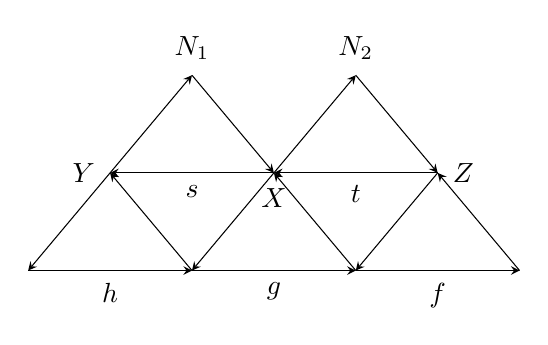
\begin{tikzpicture}[>=stealth,line width=.38pt,scale=.80]
    \coordinate (Y)  at (0,0);
    \coordinate (X)  at (2.6,0);
    \coordinate (Z)  at (5.2,0);
    \coordinate (N1) at (1.3,1.55);
    \coordinate (N2) at (3.9,1.55);
    \coordinate (A)  at (-1.3,-1.55);
    \coordinate (Q1) at (1.3,-1.55);
    \coordinate (Q2) at (3.9,-1.55);
    \coordinate (B)  at (6.5,-1.55);

    \VerdierHatchTriangle{Y}{N1}{X}
    \VerdierHatchTriangle{X}{N2}{Z}
    \VerdierHatchTriangle{Y}{A}{Q1}
    \VerdierHatchTriangle{X}{Q1}{Q2}
    \VerdierHatchTriangle{Z}{Q2}{B}

    \draw[->] (Y) -- (N1);
    \draw[->] (N1) -- (X);
    \draw[->] (X) -- node[below=1pt] {$s$} (Y);
    \draw[->] (X) -- (N2);
    \draw[->] (N2) -- (Z);
    \draw[->] (Z) -- node[below=1pt] {$t$} (X);

    \draw[->] (Y) -- (A);
    \draw[->] (A) -- node[below=1pt] {$h$} (Q1);
    \draw[->] (Q1) -- (Y);
    \draw[->] (X) -- (Q1);
    \draw[->] (Q1) -- node[below=1pt] {$g$} (Q2);
    \draw[->] (Q2) -- (X);
    \draw[->] (Z) -- (Q2);
    \draw[->] (Q2) -- node[below=1pt] {$f$} (B);
    \draw[->] (B) -- (Z);

    \node[left=2pt]  at (Y)  {$Y$};
    \node[below=2pt] at (X)  {$X$};
    \node[right=2pt] at (Z)  {$Z$};
    \node[above=2pt] at (N1) {$N_1$};
    \node[above=2pt] at (N2) {$N_2$};
  \end{tikzpicture}
  \quad ,
\end{center}

\VerdierSemanticAnchor{ch2-2-1-13-diagram-interpretation}
\noindent 其中 $N_1$ 与 $N_2$ 是 $\mathcal D'$ 的对象，五个带阴影的三角是
特异三角，两个未带阴影的三角是交换的。

\VerdierSemanticAnchor{ch2-2-1-13-shifted-zero}
由此得到 $s[1]t=0$ (1.2.2)。
\VerdierSemanticAnchor{ch2-2-1-13-shifted-membership}%
此外，由 SM1) 与 SM5)，态射 $s[1]t$ 属于 $S(\mathcal D')$。

\VerdierSemanticAnchor{ch2-2-1-13-split-triangle}
因此存在形如 $(Z,Y[2],N,0,u,v)$ 的特异三角，其中 $N$ 是 $\mathcal D'$
的对象。
\VerdierSemanticAnchor{ch2-2-1-13-direct-summand}%
由 (1.2.6) 与 TRII 可知，$Y$ 是 $\mathcal D'$ 的某个对象的直和项。
\VerdierSemanticAnchor{ch2-2-1-13-y-in-dprime}%
因此，$Y$ 同构于 $\mathcal D'$ 的一个对象。

\VerdierSemanticAnchor{ch2-2-1-13-s-triangle}
再利用 (1.2.4)、$\mathcal D'$ 是 $\mathcal D$ 的三角子范畴这一事实，以及
特异三角：

\begin{center}
  \begin{tikzpicture}[>=stealth,line width=.38pt,scale=.80]
    \coordinate (Y)  at (-2,0);
    \coordinate (X)  at (2,0);
    \coordinate (N1) at (0,1.55);
    \VerdierHatchTriangle{Y}{N1}{X}
    \draw[->] (Y) -- (N1);
    \draw[->] (N1) -- (X);
    \draw[->] (X) -- node[below=1pt] {$s$} (Y);
    \node[left=2pt]  at (Y)  {$Y$};
    \node[right=2pt] at (X)  {$X$};
    \node[above=2pt] at (N1) {$N_1$};
  \end{tikzpicture}
\end{center}

\VerdierSemanticAnchor{ch2-2-1-13-g-membership}
\noindent 可知 $X$ 同构于 $\mathcal D'$ 的一个对象。因此，态射 $g$ 属于
$S(\mathcal D')$。

\VerdierSemanticAnchor{ch2-2-1-14}
\medskip
\noindent\textbf{2.1.14.}\quad
\VerdierSemanticAnchor{ch2-2-1-14-saturation-direction}%
\emph{如果集合 $S(\mathcal D')$ 是饱和的，则子范畴 $\mathcal D'$ 是饱和的。}

\VerdierSemanticAnchor{ch2-2-1-14-direct-summand-setup}
设 $X$ 为 $\mathcal D'$ 的某个对象的直和项。
\VerdierSemanticAnchor{ch2-2-1-14-first-triangle}%
由 (1.2.6) 与 TRII 可见，存在特异三角 $(X,Y,N,0,u,v)$，其中 $N$ 是
$\mathcal D'$ 的对象。
\VerdierSemanticAnchor{ch2-2-1-14-zero-morphism}%
因此，零态射 $X\to Y$ 属于 $S(\mathcal D')$。

\VerdierSemanticAnchor{ch2-2-1-14-sm4-application}
把性质 SM4) 应用于三个态射 $0\to X\to 0\to Y$。
\VerdierSemanticAnchor{ch2-2-1-14-x-zero-membership}%
由此可知态射 $X\to 0$ 属于 $S(\mathcal D')$。

\VerdierSemanticAnchor{ch2-2-1-14-second-triangle}
因此存在特异三角 $(X,0,N,0,0,i)$，其中 $N$ 是 $\mathcal D'$ 的对象。
\VerdierSemanticAnchor{ch2-2-1-14-shift-isomorphism}%
于是态射 $N\xrightarrow{i}X[1]$ 是同构。因此 $X$ 同构于 $N[-1]$，
而后者是 $\mathcal D'$ 的对象。

\VerdierSemanticAnchor{ch2-2-1-14-proposition-complete}
这就完成了命题 (2.1.8) 的证明。

\VerdierSemanticAnchor{ch2-2-1-14-p134-boundary}
\endgroup

\VerdierSourcePageBlock{0134}%
\begingroup
\VerdierSemanticAnchor{ch2-2-1-15}
\noindent\textbf{2.1.15.}\quad
\VerdierSemanticAnchor{ch2-2-1-15-associated-system}%
设 $\mathcal D'$ 为三角范畴 $\mathcal D$ 的满三角子范畴。乘法系
$S(\mathcal D')$ (2.1.7) 称为\emph{与子范畴 $\mathcal D'$ 关联的
乘法系}。

\VerdierSemanticAnchor{ch2-2-1-16}
\smallskip
\noindent\textbf{命题 2.1.16.}\quad
\begingroup\itshape
\VerdierSemanticAnchor{ch2-2-1-16-setup}%
设 $F\colon\mathcal D_1\to\mathcal D_2$ 为两个三角范畴之间的正合
函子 (1.1.3)。以 $S(F)$ 表示 $\mathcal D_1$ 中被 $F$ 送到
$\mathcal D_2$ 的同构的态射集合。
\VerdierSemanticAnchor{ch2-2-1-16-kernel-subcategory}%
以 $\mathcal D'(F)$ 表示 $\mathcal D_1$ 的满子范畴，其对象是被
$F$ 送到 $\mathcal D_2$ 的零对象的那些 $\mathcal D_1$ 的对象。

\VerdierSemanticAnchor{ch2-2-1-16-a}
\par\noindent\hspace*{2em}a)\enspace 子范畴 $\mathcal D'(F)$ 是严格满
且饱和的三角子范畴（$\mathcal D_1$ 中每个同构于 $\mathcal D'(F)$
的某个对象的对象，都是 $\mathcal D'(F)$ 的对象）。

\VerdierSemanticAnchor{ch2-2-1-16-b}
\par\noindent\hspace*{2em}b)\enspace 集合 $S(F)$ 是 $\mathcal D_1$
的饱和乘法系。

\VerdierSemanticAnchor{ch2-2-1-16-c}
\par\noindent\hspace*{2em}c)\enspace 集合 $S(F)$ 是与子范畴
$\mathcal D'(F)$ 关联的乘法系 (2.1.15)。
\par\endgroup

\VerdierSemanticAnchor{ch2-2-1-16-proof-omitted}
\noindent 证明很容易，留给读者；读者也可用同样的方法证明下列命题：

\VerdierSemanticAnchor{ch2-2-1-17}
\smallskip
\noindent\textbf{命题 2.1.17.}\quad
\begingroup\itshape
\VerdierSemanticAnchor{ch2-2-1-17-setup}%
设 $H\colon\mathcal D\to\mathcal A$ 为从三角范畴到阿贝尔范畴的
上同调函子。以 $S(H)$ 表示 $\mathcal D$ 中连同其所有平移的像都为
$\mathcal A$ 的同构的态射集合。
\VerdierSemanticAnchor{ch2-2-1-17-kernel-subcategory}%
以 $\mathcal D'(H)$ 表示 $\mathcal D$ 的满子范畴，其对象是连同
其所有平移的像都为 $\mathcal A$ 的零对象的那些
$\mathcal D$ 的对象。

\VerdierSemanticAnchor{ch2-2-1-17-a}
\par\noindent\hspace*{2em}a)\enspace 子范畴 $\mathcal D'(H)$ 是严格满
且饱和的三角子范畴。

\VerdierSemanticAnchor{ch2-2-1-17-b}
\par\noindent\hspace*{2em}b)\enspace 集合 $S(H)$ 是 $\mathcal D$
的饱和乘法系。

\VerdierSemanticAnchor{ch2-2-1-17-c}
\par\noindent\hspace*{2em}c)\enspace 集合 $S(H)$ 是与子范畴
$\mathcal D'(H)$ 关联的乘法系 (2.1.15)。
\par\endgroup

\VerdierSemanticAnchor{ch2-2-2}
\medskip
\noindent\textbf{2.2.\quad 局部化范畴的构造。}

\VerdierSemanticAnchor{ch2-2-2-1}
\smallskip
\noindent\textbf{2.2.1.}\quad
\VerdierSemanticAnchor{ch2-2-2-1-slice-categories}%
设 $\mathcal C$ 为一个范畴（不必加性），$S$ 为 $\mathcal C$ 的乘法系。
对于 $\mathcal C$ 的每个对象 $X$，以 $S/X$（分别地，$X\backslash S$）
表示如下范畴：其对象为 $S$ 中靶为 $X$（分别地，源为 $X$）的态射，
\VerdierSemanticAnchor{ch2-2-2-1-morphism-diagrams}%
其态射为下列交换图：

\VerdierSemanticAnchor{ch2-2-2-1-s-over-x-diagram}
\begin{center}
  \begin{tikzpicture}[>=stealth,line width=.38pt,scale=.90]
    \node (Y)  at (-1.55,1.05) {$Y$};
    \node (Yp) at ( 1.55,1.05) {$Y'$};
    \node (X)  at ( 0,-.95) {$X$};
    \draw[->] (Y) -- node[above=1pt] {$u$} (Yp);
    \draw[->] (Y) -- node[left=2pt] {$s$} (X);
    \draw[->] (Yp) -- node[right=2pt] {$t$} (X);
    \node at (3.15,.05) {$s,t\in S$};
  \end{tikzpicture}
  \quad ,
\end{center}

\VerdierSemanticAnchor{ch2-2-2-1-p135-boundary}
\endgroup%
\VerdierSourcePageContinue{0135}%
\begingroup
\normalsize
\setlength{\emergencystretch}{1.5em}%
\setlength{\abovedisplayskip}{2pt plus 1pt minus 1pt}%
\setlength{\belowdisplayskip}{2pt plus 1pt minus 1pt}%

\VerdierSemanticAnchor{ch2-2-2-1-x-backslash-s-diagram}
\noindent\hspace*{.3em}（分别地\quad
\begin{tikzpicture}[>=stealth,line width=.38pt,scale=.90,
  baseline={(current bounding box.center)}]
  \node (X)  at (0,1.50) {$X$};
  \node (Y)  at (-1.30,-.55) {$Y$};
  \node (Yp) at (1.30,-.55) {$Y'$};
  \draw[->] (X) -- node[left=2pt] {$s$} (Y);
  \draw[->] (X) -- node[right=2pt] {$t$} (Yp);
  \draw[->] (Y) -- node[above=1pt] {$u$} (Yp);
  \node at (3.10,.45) {$s,t\in S$};
\end{tikzpicture}
\quad ）\,。

\VerdierSemanticAnchor{ch2-2-2-1-localized-hom-definition}
\smallskip
\noindent 对 $\mathcal C$ 的每一对对象 $X,Y$，令：

\VerdierSemanticAnchor{ch2-2-2-1-formula-2-2-1-1}
\par\smallskip
\noindent\makebox[0pt][l]{(2.2.1.1)}%
\begin{minipage}[t]{\linewidth}
  \centering
  $\displaystyle
    \operatorname{Hom}_{\mathcal C(S^{-1})}(X,Y)
    =\varinjlim_{(S/X)^{\circ}}
     \operatorname{Hom}_{\mathcal C}(\,\cdot\,,Y)\,.$
\end{minipage}
\par\smallskip

\VerdierSemanticAnchor{ch2-2-2-1-dot-explanation}
\noindent （公式 (2.2.1.1) 中的“点”表示 $S/X$ 的一个可变对象的源）。

\VerdierSemanticAnchor{ch2-2-2-1-filtered-category}
由性质 SM1)、SM2) 与 SM3) 立即可知，范畴 $(S/X)^{\circ}$ 是滤过的 [6]。
\VerdierSemanticAnchor{ch2-2-2-1-roof-class}%
因此，$\operatorname{Hom}_{\mathcal C(S^{-1})}(X,Y)$ 的一个元素是形如
下列图式的一个等价类：

\VerdierSemanticAnchor{ch2-2-2-1-roof-formula}
\[
  D=X\xleftarrow{s}X'\xrightarrow{m}Y,\qquad s\in S,
\]

\VerdierSemanticAnchor{ch2-2-2-1-equivalence-setup}
\noindent 两个图式
$D_1=X\xleftarrow{s_1}X_1\xrightarrow{m_1}Y$ 与
$D_2=X\xleftarrow{s_2}X_2\xrightarrow{m_2}Y$ 属于同一等价类，当且仅当
存在图式：

\VerdierSemanticAnchor{ch2-2-2-1-common-refinement-roof}
\[
  D_3=X\xleftarrow{s_3}X_3\xrightarrow{m_3}Y,\qquad s_3\in S,
\]

\VerdierSemanticAnchor{ch2-2-2-1-common-refinement-diagram-introduction}
\noindent 以及交换图：

\VerdierSemanticAnchor{ch2-2-2-1-common-refinement-diagram}
\begin{center}
  \begin{tikzpicture}[>=stealth,line width=.38pt,x=1.45cm,y=1.02cm,
    scale=.95]
    \node (X1) at (0,1.35) {$X_1$};
    \node (X3) at (0,0) {$X_3$};
    \node (X2) at (0,-1.35) {$X_2$};
    \node (X)  at (-2.15,0) {$X$};
    \node (Y)  at (2.15,0) {$Y$};
    \draw[->] (X1) -- node[above left=-1pt] {$s_1$} (X);
    \draw[->] (X3) -- node[above=1pt] {$s_3$} (X);
    \draw[->] (X2) -- node[below left=-1pt] {$s_2$} (X);
    \draw[->] (X3) -- node[right=1pt] {$u$} (X1);
    \draw[->] (X3) -- node[right=1pt] {$v$} (X2);
    \draw[->] (X1) -- node[above right=-1pt] {$m_1$} (Y);
    \draw[->] (X3) -- node[above=1pt] {$m_3$} (Y);
    \draw[->] (X2) -- node[below right=-1pt] {$m_2$} (Y);
  \end{tikzpicture}
  \quad .
\end{center}

\VerdierSemanticAnchor{ch2-2-2-1-q-of-f}
\noindent 对每个元素 $f\in\operatorname{Hom}_{\mathcal C}(X,Y)$，以
$Q(f)$ 表示图式 $X\xleftarrow{\operatorname{id}_X}X\xrightarrow{f}Y$
的等价类。
\VerdierSemanticAnchor{ch2-2-2-1-q-of-s-inverse}%
对每个态射 $s\colon Y\to X$，$s\in S$，以 $Q(s)^{-1}$ 表示图式
$X\xleftarrow{s}Y\xrightarrow{\operatorname{id}_Y}Y$ 的等价类。

\VerdierSemanticAnchor{ch2-2-2-1-fl-morphism-set}
再以 $\operatorname{Fl}(\mathcal C(S^{-1}))$ 表示集合：

\VerdierSemanticAnchor{ch2-2-2-1-fl-product-formula}
\[
  \prod_{(X,Y)\in\operatorname{Ob}(\mathcal C)\times\operatorname{Ob}(\mathcal C)}
  \operatorname{Hom}_{\mathcal C(S^{-1})}(X,Y),
\]

\VerdierSemanticAnchor{ch2-2-2-1-p136-boundary}
\endgroup%
\VerdierSourcePageContinue{0136}%
\begingroup
\VerdierSemanticAnchor{ch2-2-2-1-fl-source-target-maps}
\noindent 以 $\mathbf{s}$ 与 $\mathbf{b}\colon
\operatorname{Fl}(\mathcal C(S^{-1}))\rightrightarrows
\operatorname{Ob}(\mathcal C)$ 表示映射：

\VerdierSemanticAnchor{ch2-2-2-1-source-target-formula}
\[
  m\in\operatorname{Hom}_{\mathcal C(S^{-1})}(X,Y),\qquad
  \mathbf{s}(m)=X,\qquad \mathbf{b}(m)=Y,
\]

\VerdierSemanticAnchor{ch2-2-2-1-identity-map}
\noindent 并以 $\mathbf{id}\colon\operatorname{Ob}(\mathcal C)
\to\operatorname{Fl}(\mathcal C(S^{-1}))$ 表示映射
$X\mapsto Q(\mathbf{id}_X)$。
\VerdierSemanticAnchor{ch2-2-2-1-category-diagram}%
由此定义图式
\[
\mathcal C(S^{-1})=(\operatorname{Ob}(\mathcal C),
\operatorname{Fl}(\mathcal C(S^{-1})),\mathbf{s},\mathbf{b},\mathbf{id})
\]。
此外还有一对滥用记号表示为下式的映射：

\VerdierSemanticAnchor{ch2-2-2-1-q-pair}
\[
  Q=\bigl(\mathbf{id}_{\operatorname{Ob}(\mathcal C)}\colon
  \operatorname{Ob}(\mathcal C)\to\operatorname{Ob}(\mathcal C),\;
  Q\colon\operatorname{Fl}(\mathcal C)\to
  \operatorname{Fl}(\mathcal C(S^{-1}))\bigr)\,.
\]

\VerdierSemanticAnchor{ch2-2-2-2}
\smallskip
\noindent\textbf{定理 2.2.2.}\quad
\begingroup\itshape
\VerdierSemanticAnchor{ch2-2-2-2-a}%
a) 在 $\operatorname{Fl}(\mathcal C(S^{-1}))$ 上存在唯一的部分定义的
复合法则，使得：

\VerdierSemanticAnchor{ch2-2-2-2-a-1}
\par\noindent\hspace*{2em}1) $\mathcal C(S^{-1})$ 是一个范畴。

\VerdierSemanticAnchor{ch2-2-2-2-a-2}
\par\noindent\hspace*{2em}2) $Q(s)$ 是同构，且 $Q(s)^{-1}$ 是其逆
$(s\in S)$。

\VerdierSemanticAnchor{ch2-2-2-2-a-3}
\par\noindent\hspace*{2em}3) 对每个图式
$D=X\xleftarrow{s}X'\xrightarrow{m}Y$，$s\in S$，都有
$\overline D=Q(m)Q(s)^{-1}$
$(\overline D\in\operatorname{Hom}_{\mathcal C(S^{-1})}(X,Y)$ 是
$D$ 的等价类）。

\VerdierSemanticAnchor{ch2-2-2-2-a-4}
\par\noindent\hspace*{2em}4) $Q$ 是一个函子。

\VerdierSemanticAnchor{ch2-2-2-2-b}
\par\noindent b) $\mathcal C(S^{-1})$ 的每个态射都可写成复合
$Q(t)^{-1}Q(m)$，其中 $m\in\operatorname{Fl}(\mathcal C)$、$t\in S$
（分别地，写成 $Q(p)Q(s)^{-1}$，其中
$p\in\operatorname{Fl}(\mathcal C)$、$s\in S$）。

\VerdierSemanticAnchor{ch2-2-2-2-c}
\par\noindent c) 函子 $Q$ 与有限射影极限及有限归纳极限可交换。

\VerdierSemanticAnchor{ch2-2-2-2-d}
\par\noindent d) 对每个范畴 $\mathcal A$，与函子 $Q$ 的复合定义函子：

\VerdierSemanticAnchor{ch2-2-2-2-hom-q-a}
\[
  \mathcal{H}\!om(Q,\mathcal A)\colon
  \mathcal{H}\!om(\mathcal C(S^{-1}),\mathcal A)
  \longrightarrow \mathcal{H}\!om(\mathcal C,\mathcal A)
\]

\noindent\textup{（$\mathcal{H}\!om$ 表示函子范畴）。}
\VerdierSemanticAnchor{ch2-2-2-2-universal-image}%
函子 $\mathcal{H}\!om(Q,\mathcal A)$ 在对象上单射且充分忠实；
$\mathcal{H}\!om(\mathcal C(S^{-1}),\mathcal A)$ 的像，是
$\mathcal{H}\!om(\mathcal C,\mathcal A)$ 的严格满子范畴，其对象是
那些把 $S$ 中的态射送到同构的从 $\mathcal C$ 到 $\mathcal A$ 的函子。
\par\endgroup

\VerdierSemanticAnchor{ch2-2-2-2-proof-omitted}
该定理的证明留给读者；读者可参阅 [16]。
\VerdierSemanticAnchor{ch2-2-2-2-composition-setup}%
这里只描述 $\mathcal C(S^{-1})$ 中态射的复合。设
$\overline D_1\in\operatorname{Hom}_{\mathcal C(S^{-1})}(X,Y)$ 与
$\overline D_2\in\operatorname{Hom}_{\mathcal C(S^{-1})}(Y,Z)$ 为
$\mathcal C(S^{-1})$ 中两个可复合的态射。

\VerdierSemanticAnchor{ch2-2-2-2-roof-pair}
设 $D_1=X\xleftarrow{s}X'\xrightarrow{m}Y$ 与
$D_2=Y\xleftarrow{t}Y'\xrightarrow{p}Z$ 为 $\mathcal C$ 中分别属于
$\overline D_1$ 与 $\overline D_2$ 的两个图式。
\VerdierSemanticAnchor{ch2-2-2-2-sm2-completion-input}%
利用 SM2)，把图式

\begin{center}
  \begin{tikzpicture}[>=stealth,line width=.38pt,x=1.42cm,y=.90cm,
    scale=.92]
    \node (Xp) at (-1.20,1.10) {$X'$};
    \node (Yp) at ( 1.20,1.10) {$Y'$};
    \node (Y)  at ( 0,-.70) {$Y$};
    \draw[->] (Xp) -- node[left=2pt] {$m$} (Y);
    \draw[->] (Yp) -- node[right=2pt] {$t$} (Y);
    \node at (3.00,.25) {$t\in S$};
  \end{tikzpicture}
\end{center}

\VerdierSemanticAnchor{ch2-2-2-2-p137-boundary}
\endgroup%
\VerdierSourcePageContinue{0137}%
\begingroup
\VerdierSemanticAnchor{ch2-2-2-2-sm2-completion-diagram}
\noindent 补成如下交换图：

\begin{center}
  \begin{tikzpicture}[>=stealth,line width=.38pt,x=1.30cm,y=1.45cm,
    scale=.92]
    \node (Zpp) at (0,2.20) {$Z''$};
    \node (Xp)  at (-1.25,1.10) {$X'$};
    \node (Yp)  at ( 1.25,1.10) {$Y'$};
    \node (Y)   at (0,0) {$Y$};
    \draw[->] (Zpp) -- node[above left=-1pt] {$t'\in S$} (Xp);
    \draw[->] (Zpp) -- node[above right=-1pt] {$m'$} (Yp);
    \draw[->] (Xp)  -- node[below left=-1pt] {$m$} (Y);
    \draw[->] (Yp)  -- node[below right=-1pt] {$t\in S$} (Y);
    \node at (2.50,-.05) {$.$};
  \end{tikzpicture}
\end{center}

\VerdierSemanticAnchor{ch2-2-2-2-composite-roof-d3}
\noindent 于是得到图式
$D_3=X\xleftarrow{st'}Z''\xrightarrow{pm'}Z$，其中复合态射 $st'$ 属于
$S$ (SM1)。
\VerdierSemanticAnchor{ch2-2-2-2-composite-class-independence}%
可以验证，$D_3$ 在
$\operatorname{Hom}_{\mathcal C(S^{-1})}(X,Z)$ 中的类
$\overline D_3$ 只依赖于类 $\overline D_1$ 与 $\overline D_2$。
\VerdierSemanticAnchor{ch2-2-2-2-composition-conclusion}%
态射 $\overline D_3$ 就是 $\mathcal C(S^{-1})$ 中态射
$\overline D_1$ 与 $\overline D_2$ 的复合。

\VerdierSemanticAnchor{ch2-2-2-3}
\smallskip
\noindent\textbf{注 2.2.3.}
\VerdierSemanticAnchor{ch2-2-2-3-a}%
a) 由定理 (2.2.2) 的第四个断言可知，配备函子
$Q\colon\mathcal C\longrightarrow\mathcal C(S^{-1})$ 的范畴
$\mathcal C(S^{-1})$ 是一个泛问题的解：
\VerdierSemanticAnchor{ch2-2-2-3-a-universal-problem}%
函子 $Q$ 把 $S$ 中的态射送到同构；而从 $\mathcal C$ 到某个范畴
$\mathcal A$、并把 $S$ 中态射送到同构的每个函子，都唯一地通过
$Q$ 分解。
\VerdierSemanticAnchor{ch2-2-2-3-a-unique-isomorphism}%
因此，由这一性质，配备函子 $Q$ 的范畴 $\mathcal C(S^{-1})$ 在唯一
同构意义下确定。

\VerdierSemanticAnchor{ch2-2-2-3-b}
\par\noindent b) 设 $\mathcal C$ 为范畴，$S$ 为 $\mathcal C$ 的一个态射
集合，不要求它是 $\mathcal C$ 的乘法系。
\VerdierSemanticAnchor{ch2-2-2-3-b-general-localization}%
总存在范畴 $\mathcal C(S^{-1})$ 以及把 $S$ 中态射送到同构的函子
$Q\colon\mathcal C\longrightarrow\mathcal C(S^{-1})$，使得从
$\mathcal C$ 到某个范畴 $\mathcal A$、并把 $S$ 中态射送到同构的
每个函子，都唯一地通过 $Q$ 分解。
\VerdierSemanticAnchor{ch2-2-2-3-b-multiplicative-comparison}%
当 $S$ 是 $\mathcal C$ 的乘法系时，定理 (2.2.2) 给出范畴
$\mathcal C(S^{-1})$ 的一个简单描述；它还给出函子 $Q$ 的若干附加
性质（断言 b) 与 c)），这些性质在一般情形下并不成立。

\VerdierSemanticAnchor{ch2-2-2-4}
\smallskip
\noindent\textbf{推论 2.2.4.}\quad
\begingroup\itshape
设 $\mathcal C$ 为范畴，$S$ 为 $\mathcal C$ 的乘法系。

\VerdierSemanticAnchor{ch2-2-2-4-a}
\par\noindent a) 集合 $S$ 是 $\mathcal C$ 的反范畴
$\mathcal C^\circ$ 的乘法系。
\VerdierSemanticAnchor{ch2-2-2-4-a-opposite-system}%
存在范畴的典范同构：

\VerdierSemanticAnchor{ch2-2-2-4-a-canonical-isomorphism}
\[
  \bigl(\mathcal C^\circ(S^{-1})\bigr)^\circ
  \longrightarrow \mathcal C(S^{-1})\,.
\]

\VerdierSemanticAnchor{ch2-2-2-4-a-hom-colimit-isomorphism}
\noindent 特别地，该同构诱导同构：
\[
  \operatorname{Hom}_{\mathcal C(S^{-1})}(X,Y)
  \longrightarrow
  \varinjlim_{Y\backslash S}\operatorname{Hom}_{\mathcal C}(X,\mathord\cdot)\,.
\]
\endgroup

\VerdierSemanticAnchor{ch2-2-2-4-p138-boundary}
\endgroup%
\VerdierSourcePageContinue{0138}%
\begingroup
\begingroup\itshape
\VerdierSemanticAnchor{ch2-2-2-4-b}
\noindent b) 当范畴 $\mathcal C$ 是加性范畴时，范畴
$\mathcal C(S^{-1})$ 是加性范畴，且函子 $Q$ 是加性函子。

\VerdierSemanticAnchor{ch2-2-2-4-c}
\par\noindent c) 设 $\widehat S$ 为 $\mathcal C$ 中被 $Q$ 送到
$\mathcal C(S^{-1})$ 的同构的态射集合。
\VerdierSemanticAnchor{ch2-2-2-4-c-saturation}%
集合 $\widehat S$ 是 $\mathcal C$ 的饱和乘法系。$\mathcal C$ 中每个
包含 $S$ 的饱和乘法系都包含 $\widehat S$。
\endgroup

\VerdierSemanticAnchor{ch2-2-2-4-proof-b}
\par\noindent 第一个断言立即由 $\mathcal C(S^{-1})$ 的泛性质得到：
范畴 $\bigl(\mathcal C^\circ(S^{-1})\bigr)^\circ$ 是该泛问题的一个解。
第二个断言立即由定理 (2.2.2) 的断言 b) 与 c) 得到。
\VerdierSemanticAnchor{ch2-2-2-4-proof-c-characterization}%
由 $\mathcal C(S^{-1})$ 中态射的描述立即可知，$\mathcal C$ 的态射
$f$ 被 $Q$ 送到同构，当且仅当 $\mathcal C$ 中存在两个态射 $g$ 与
$h$，使得 $gf$ 与 $fh$ 有定义并且属于 $S$。
\VerdierSemanticAnchor{ch2-2-2-4-proof-c-sm2-sm3}%
由此立即可知，集合 $\widehat S$ 具有性质 SM2) 与 SM3)。
\VerdierSemanticAnchor{ch2-2-2-4-proof-c-sm1-sm4}%
此外，由 $\widehat S$ 的定义可知，该集合具有性质 SM1) 与 SM4)。
\VerdierSemanticAnchor{ch2-2-2-4-proof-c-conclusion}%
因此，$\widehat S$ 是 $\mathcal C$ 的饱和乘法系。(2.2.4) 的最后一个
断言是显然的。

\VerdierSemanticAnchor{ch2-2-2-5}
\smallskip
\noindent\textbf{2.2.5.} 设 $\mathcal C$ 为范畴，$S$ 为
$\mathcal C$ 的乘法系。
\VerdierSemanticAnchor{ch2-2-2-5-localized-category}%
范畴 $\mathcal C(S^{-1})$ 称为 $\mathcal C$ 关于乘法系 $S$ 的
\emph{局部化范畴}。
\VerdierSemanticAnchor{ch2-2-2-5-localization-functor}%
函子 $Q\colon\mathcal C\longrightarrow\mathcal C(S^{-1})$ 称为
\emph{局部化函子}。
\VerdierSemanticAnchor{ch2-2-2-5-saturation}%
乘法系 $\widehat S$ 称为乘法系 $S$ 的\emph{饱和化}。

\VerdierSemanticAnchor{ch2-2-2-6}
\smallskip
\noindent\textbf{定理 2.2.6.}\quad
\begingroup\itshape
\VerdierSemanticAnchor{ch2-2-2-6-setup}%
设 $\mathcal D$ 为三角范畴，$S$ 为 $\mathcal D$ 的乘法系 (2.1.4)。
以 $\mathcal D(S^{-1})$ 表示 $\mathcal D$ 的局部化范畴，以
$Q\colon\mathcal D\longrightarrow\mathcal D(S^{-1})$ 表示局部化函子。

\VerdierSemanticAnchor{ch2-2-2-6-a}
\par\noindent a) 在 $\mathcal D(S^{-1})$ 上存在唯一的严格
$\mathbb Z$-范畴结构，使 $Q$ 为严格 $\mathbb Z$-函子。

\VerdierSemanticAnchor{ch2-2-2-6-b}
\par\noindent b) 在 $\mathcal D(S^{-1})$ 上存在唯一的三角结构，使
$Q$ 为正合函子。该结构的特异三角，是那些同构于 $\mathcal D$ 的
特异三角在 $Q$ 下的像的三角。

\VerdierSemanticAnchor{ch2-2-2-6-c-factorization}
\par\noindent c) 到某个三角范畴（分别地，阿贝尔范畴）、并把 $S$
中态射送到同构的每个正合（分别地，上同调）函子
$F\colon\mathcal D\longrightarrow\mathcal D'$，都唯一地通过
$Q\colon\mathcal D\longrightarrow\mathcal D(S^{-1})$ 分解为正合
（分别地，上同调）函子
$G\colon\mathcal D(S^{-1})\longrightarrow\mathcal D'$。
\VerdierSemanticAnchor{ch2-2-2-6-c-morphism-lifting}%
设 $F_1,F_2\colon\mathcal D\rightrightarrows\mathcal D'$ 为两个把
$S$ 中态射送到同构的正合（分别地，上同调）函子；设
$G_1,G_2\colon\mathcal D(S^{-1})\rightrightarrows\mathcal D'$ 为它们
各自的分解，并设 $m\colon F_1\longrightarrow F_2$ 为正合（分别地，
上同调）函子的态射。存在唯一的函子态射
$p\colon G_1\longrightarrow G_2$，使 $m=p\star Q$。
\endgroup

\VerdierSemanticAnchor{ch2-2-2-6-proof-a}
\par\noindent 第一个断言立即由定理 (2.2.2) 与 SM5) 得到。
\VerdierSemanticAnchor{ch2-2-2-6-proof-c-p139-boundary}%
第三个断言立即由

\VerdierSemanticAnchor{ch2-2-2-6-p139-boundary}
\endgroup%
\VerdierSourcePageContinue{0139}%
\begingroup
\normalsize
\setlength{\parskip}{0pt}%
\setlength{\emergencystretch}{1.5em}%
\setlength{\abovedisplayskip}{1pt plus 1pt minus 1pt}%
\setlength{\belowdisplayskip}{1pt plus 1pt minus 1pt}%

\VerdierSemanticAnchor{ch2-2-2-6-proof-c-continuation}
\noindent 第二个断言与定理 (2.2.2) 得到。因此尚需证明第二个断言。
\VerdierSemanticAnchor{ch2-2-2-6-proof-b-setup}%
设 $T$ 为 $\mathcal D(S^{-1})$ 中那些同构于 $\mathcal D$ 的特异三角
在 $Q$ 下的像的三角所成的集合。
\VerdierSemanticAnchor{ch2-2-2-6-proof-b-tri-trii}%
不难验证，集合 $T$ 具有性质 TRI 与 TRII。为证明它具有性质 TRIII，
我们需要下述引理：

\VerdierSemanticAnchor{ch2-2-2-7}
\smallskip
\noindent\textbf{引理 2.2.7.}\quad
\begingroup\itshape
设 $u\colon X\longrightarrow Y$ 与 $u'\colon X'\longrightarrow Y'$ 为
$\mathcal D$ 的两个态射，并设

\VerdierSemanticAnchor{ch2-2-2-7-localized-square}
\begin{center}
  \begin{tikzpicture}[>=stealth,line width=.38pt,x=1.70cm,y=1.25cm,
    scale=.98]
    \node (QX)  at (0,1) {$Q(X)$};
    \node (QY)  at (2.35,1) {$Q(Y)$};
    \node (QXp) at (0,0) {$Q(X')$};
    \node (QYp) at (2.35,0) {$Q(Y')$};
    \draw[->] (QX) -- node[above] {$Q(u)$} (QY);
    \draw[->] (QXp) -- node[below] {$Q(u')$} (QYp);
    \draw[->] (QX) -- node[left] {$m$} (QXp);
    \draw[->] (QY) -- node[right] {$p$} (QYp);
  \end{tikzpicture}
\end{center}

\noindent 为 $\mathcal D(S^{-1})$ 中的交换图。
\VerdierSemanticAnchor{ch2-2-2-7-common-representative}%
则存在态射 $u''\colon X''\longrightarrow Y''$，以及 $\mathcal D$ 中的
两个交换图：

\begin{center}
  \VerdierSemanticAnchor{ch2-2-2-7-denominator-square}%
  \begin{tikzpicture}[>=stealth,line width=.38pt,x=1.55cm,y=1.15cm,
    scale=.95]
    \node (Xpp) at (0,1) {$X''$};
    \node (Ypp) at (2,1) {$Y''$};
    \node (X)   at (0,0) {$X$};
    \node (Y)   at (2,0) {$Y$};
    \draw[->] (Xpp) -- node[above] {$u''$} (Ypp);
    \draw[->] (X) -- node[below] {$u$} (Y);
    \draw[->] (Xpp) -- node[left] {$s$} (X);
    \draw[->] (Ypp) -- node[right] {$t$} (Y);
    \node at (3.25,.50) {$s,t\in S$};
    \node at (4.50,0) {$,$};
  \end{tikzpicture}
  \par\smallskip
  \VerdierSemanticAnchor{ch2-2-2-7-numerator-square}%
  \begin{tikzpicture}[>=stealth,line width=.38pt,x=1.55cm,y=1.15cm,
    scale=.95]
    \node (Xpp) at (0,1) {$X''$};
    \node (Ypp) at (2,1) {$Y''$};
    \node (Xp)  at (0,0) {$X'$};
    \node (Yp)  at (2,0) {$Y'$};
    \draw[->] (Xpp) -- node[above] {$u''$} (Ypp);
    \draw[->] (Xp) -- node[below] {$u'$} (Yp);
    \draw[->] (Xpp) -- node[left] {$f$} (Xp);
    \draw[->] (Ypp) -- node[right] {$g$} (Yp);
    \node at (3.10,0) {$,$};
  \end{tikzpicture}
\end{center}

\VerdierSemanticAnchor{ch2-2-2-7-fraction-identities}
\noindent 使得 $m=Q(f)Q(s)^{-1}$ 且 $p=Q(g)Q(t)^{-1}$。
\endgroup

\VerdierSemanticAnchor{ch2-2-2-6-proof-b-triii-reduction}
\par\noindent 暂且承认该引理，并证明集合 $T$ 具有性质 TRIII。利用
集合 $T$ 的定义，问题归结为证明如下断言：给定 $\mathcal D$ 的两个
特异三角：

\VerdierSemanticAnchor{ch2-2-2-6-proof-b-distinguished-triangles}
\[
  (X,Y,Z,u,v,w)\,,\qquad
  (X',Y',Z',u',v',w')
\]

\noindent 以及 $\mathcal D(S^{-1})$ 中的交换图：

\VerdierSemanticAnchor{ch2-2-2-6-proof-b-localized-square}
\begin{center}
  \begin{tikzpicture}[>=stealth,line width=.38pt,x=1.70cm,y=1.25cm,
    scale=.98]
    \node (QX)  at (0,1) {$Q(X)$};
    \node (QY)  at (2.35,1) {$Q(Y)$};
    \node (QXp) at (0,0) {$Q(X')$};
    \node (QYp) at (2.35,0) {$Q(Y')$};
    \draw[->] (QX) -- node[above] {$Q(u)$} (QY);
    \draw[->] (QXp) -- node[below] {$Q(u')$} (QYp);
    \draw[->] (QX) -- node[left] {$m$} (QXp);
    \draw[->] (QY) -- node[right] {$p$} (QYp);
    \node at (3.05,0) {$,$};
  \end{tikzpicture}
\end{center}

\VerdierSemanticAnchor{ch2-2-2-6-proof-b-p140-boundary}
\VerdierSemanticAnchor{ch2-2-2-6-p140-boundary}
\endgroup%
\VerdierSourcePageContinue{0140}%
\begingroup
\normalsize
\setlength{\parskip}{0pt}%
\setlength{\emergencystretch}{1.5em}%
\setlength{\abovedisplayskip}{1pt plus 1pt minus 1pt}%
\setlength{\belowdisplayskip}{1pt plus 1pt minus 1pt}%

\VerdierSemanticAnchor{ch2-2-2-6-proof-b-triii-completion}
\noindent 则存在态射 $r\colon Q(Z)\longrightarrow Q(Z')$，使
$(m,p,r)$ 为三角的态射。
\VerdierSemanticAnchor{ch2-2-2-6-proof-b-triii-case-reduction}%
利用引理 (2.2.7)，问题归结为考察下列两种情形：

\VerdierSemanticAnchor{ch2-2-2-6-proof-b-triii-case-a}
\noindent\textit{a)}\quad
$m=Q(s)^{-1}$，$p=Q(t)^{-1}$，$s,t\in S$，且图式：

\VerdierSemanticAnchor{ch2-2-2-6-proof-b-triii-case-a-square}
\begin{center}
  \begin{tikzpicture}[>=stealth,line width=.38pt,x=1.85cm,y=1.45cm,
    scale=1.04]
    \node (Xp) at (0,1) {$X'$};
    \node (Yp) at (2,1) {$Y'$};
    \node (X)  at (0,0) {$X$};
    \node (Y)  at (2,0) {$Y$};
    \draw[->] (Xp) -- node[above] {$u'$} (Yp);
    \draw[->] (Xp) -- node[left] {$s$} (X);
    \draw[->] (Yp) -- node[right] {$t$} (Y);
    \draw[->] (X) -- node[below] {$u$} (Y);
  \end{tikzpicture}
\end{center}

\noindent 交换。

\VerdierSemanticAnchor{ch2-2-2-6-proof-b-triii-case-b}
\noindent\textit{b)}\quad
$m=Q(f)$，$p=Q(g)$，且图式：

\VerdierSemanticAnchor{ch2-2-2-6-proof-b-triii-case-b-square}
\begin{center}
  \begin{tikzpicture}[>=stealth,line width=.38pt,x=1.85cm,y=1.45cm,
    scale=1.04]
    \node (X)  at (0,1) {$X$};
    \node (Y)  at (2,1) {$Y$};
    \node (Xp) at (0,0) {$X'$};
    \node (Yp) at (2,0) {$Y'$};
    \draw[->] (X) -- node[above] {$u$} (Y);
    \draw[->] (X) -- node[left] {$f$} (Xp);
    \draw[->] (Y) -- node[right] {$g$} (Yp);
    \draw[->] (Xp) -- node[below] {$u'$} (Yp);
  \end{tikzpicture}
\end{center}

\noindent 交换。

\VerdierSemanticAnchor{ch2-2-2-6-proof-b-triii-case-conclusion}
\noindent 在情形 \textit{a)} 中，所需性质由性质 SM6) (2.1.2) 得到。
在情形 \textit{b)} 中，所需性质由 $\mathcal D$ 的特异三角的性质
TRIII 得到。

\VerdierSemanticAnchor{ch2-2-2-8}
\smallskip
\noindent\textbf{2.2.8.\quad 引理 2.2.7 的证明。}
\VerdierSemanticAnchor{ch2-2-2-8-initial-lift}%
由定理 (2.2.2)，存在态射 $t\colon Y''\longrightarrow Y$，$t\in S$，
使 $pQ(t)=Q(g)$，其中 $g\colon Y''\longrightarrow Y'$。然后逐步构造
下列图式：

\VerdierSemanticAnchor{ch2-2-2-8-stepwise-diagram}
\begin{center}
  \begin{tikzpicture}[>=stealth,line width=.38pt,x=1.80cm,y=1.45cm,
    scale=1.04]
    \node (Xpp)  at (0,3) {$X''$};
    \node (X2pp) at (0,2) {$X_2''$};
    \node (X1pp) at (0,1) {$X_1''$};
    \node (X)    at (0,0) {$X$};
    \node (Ypp)  at (2.35,1) {$Y''$};
    \node (Y)    at (2.35,0) {$Y$};
    \draw[->] (Xpp) -- node[left] {$s_3$} (X2pp);
    \draw[->] (X2pp) -- node[left] {$s_2$} (X1pp);
    \draw[->] (X1pp) -- node[left] {$s_1$} (X);
    \draw[->] (Xpp) -- node[pos=.58,above right] {$u''$} (Ypp);
    \draw[->] (X2pp) -- node[pos=.58,above] {$u_2''$} (Ypp);
    \draw[->] (X1pp) -- node[below] {$u_1''$} (Ypp);
    \draw[->] (Ypp) -- node[right] {$t$} (Y);
    \draw[->] (X) -- node[below] {$u$} (Y);
    \node at (3.15,0) {$,$};
  \end{tikzpicture}
\end{center}

\VerdierSemanticAnchor{ch2-2-2-8-proof-p141-boundary}
\VerdierSemanticAnchor{ch2-2-2-8-p141-boundary}
\endgroup%
\VerdierSourcePageContinue{0141}%
\begingroup
\VerdierSemanticAnchor{ch2-2-2-8-stepwise-conditions}
\noindent 使得：

\VerdierSemanticAnchor{ch2-2-2-8-condition-1}
\par\noindent\makebox[1.8em][l]{1)}$us_1=tu_1''$ 且 $s_1\in S$。
这是利用 SM2) 完成的。

\VerdierSemanticAnchor{ch2-2-2-8-condition-2}
\par\noindent\makebox[1.8em][l]{2)}$mQ(s_1s_2)=Q(f')$，其中
$f'\colon X_2''\longrightarrow X'$ 是 $\mathcal D$ 的态射，
$u_2''=u_1''s_2$，且 $s_2\in S$。这是利用定理 (2.2.2) 完成的。

\VerdierSemanticAnchor{ch2-2-2-8-condition-3}
\par\noindent\makebox[1.8em][l]{3)}$u'f's_3=gu_2''s_3$，
$u''=u_2''s_3$，且 $s_3\in S$。事实上，$\mathcal D$ 中的图式：

\VerdierSemanticAnchor{ch2-2-2-8-source-square}
\begin{center}
  \begin{tikzpicture}[>=stealth,line width=.38pt,x=1.85cm,y=1.10cm,
    scale=.96]
    \node (X2pp) at (0,1) {$X_2''$};
    \node (Ypp)  at (2,1) {$Y''$};
    \node (Xp)   at (0,0) {$X'$};
    \node (Yp)   at (2,0) {$Y'$};
    \draw[->] (X2pp) -- node[above] {$u_2''$} (Ypp);
    \draw[->] (X2pp) -- node[left] {$f'$} (Xp);
    \draw[->] (Ypp)  -- node[right] {$g$} (Yp);
    \draw[->] (Xp)   -- node[below] {$u'$} (Yp);
  \end{tikzpicture}
\end{center}

\VerdierSemanticAnchor{ch2-2-2-8-localized-commutativity}
\noindent 不一定交换。然而，对上述图式应用函子 $Q$ 所得的
$\mathcal D(S^{-1})$ 中的图式是交换的。因此有
$Q(u'f')=Q(gu_2'')\colon Q(X_2'')\longrightarrow Q(Y')$。

\VerdierSemanticAnchor{ch2-2-2-8-s3-refinement}
由 $\mathcal D(S^{-1})$ 中态射的定义，存在态射
$s_3\in S\colon X''\longrightarrow X_2''$，使
$u'f's_3=gu_2''s_3$。

\VerdierSemanticAnchor{ch2-2-2-8-proof-complete}
为完成引理的证明，只需令 $f=f's_3$，$s=s_1s_2s_3$。

\VerdierSemanticAnchor{ch2-2-2-9}
\smallskip
\noindent\textbf{2.2.9. 定理 2.2.6 证明的完成。}
\VerdierSemanticAnchor{ch2-2-2-9-triv-reduction}%
尚需证明集合 $T$ 具有性质 TRIV。现在已知该集合具有性质 TRI、TRII
与 TRIII。因此可以使用 1.2 的结果 (1.2.14)。特别地，由 (1.2.4)
可知，$T$ 中所有包含给定态射的三角彼此同构。于是，利用与命题
(1.3.2) 的证明中所用的归约类似的归约，对性质 TRIV 的证明可归结为
$\mathcal D(S^{-1})$ 中那些由 $\mathcal D$ 中的类似图式在 $Q$ 下的像
所得的图式。

\VerdierSemanticAnchor{ch2-2-2-9-reader-details}
此时验证是容易的。细节留给读者。

\VerdierSemanticAnchor{ch2-2-2-10}
\smallskip
\noindent\textbf{2.2.10.}\quad
设 $\mathcal D$ 为三角范畴，
$\mathcal B\subseteq\mathcal D$ 为满三角子范畴，$S(\mathcal B)$ 为
与 $\mathcal B$ 关联的乘法系 (2.1.15)。

\VerdierSemanticAnchor{ch2-2-2-10-quotient-category}
以 $\mathcal D/\mathcal B$ 表示范畴
$\mathcal D(S(\mathcal B)^{-1})$。范畴 $\mathcal D/\mathcal B$ 称为
\emph{$\mathcal D$ 关于 $\mathcal B$ 的商范畴}。

\VerdierSemanticAnchor{ch2-2-2-10-quotient-functor}
典范函子 $Q\colon\mathcal D\longrightarrow\mathcal D/\mathcal B$ 称为
\emph{商函子}。设 $F\colon\mathcal D\longrightarrow\mathcal D'$ 为到
某个三角范畴（分别地，阿贝尔范畴）的正合（分别地，上同调）函子。

\VerdierSemanticAnchor{ch2-2-2-10-kernel}
以 $\operatorname{Ker}(F)$ 表示由那些被 $F$ 送到零对象（分别地，
其所有平移都被 $F$ 送到零对象）的对象所定义的严格满且饱和的三角
子范畴，并称之为\emph{$F$ 的核}（(2.1.16) 与 (2.1.17)）。

\VerdierSemanticAnchor{ch2-2-2-10-p142-boundary}
\endgroup

\VerdierSourcePageBlock{0142}%
\begingroup
\VerdierSemanticAnchor{ch2-2-2-11}
\noindent\textbf{推论 2.2.11.}\quad
\begingroup\itshape
\VerdierSemanticAnchor{ch2-2-2-11-setup}%
设 $\mathcal D$ 为三角范畴，
$\mathcal B\subset\mathcal D$ 为满三角子范畴。

\VerdierSemanticAnchor{ch2-2-2-11-a}
\par\noindent a) 商函子
$Q\colon\mathcal D\longrightarrow\mathcal D/\mathcal B$ 的核，是包含
$\mathcal B$ 的最小严格满且饱和的三角子范畴。

\VerdierSemanticAnchor{ch2-2-2-11-b-order-isomorphism}
\par\noindent b) 映射 $\mathcal B\longmapsto S(\mathcal B)$ 把每个
严格满且饱和的三角子范畴对应到它的饱和乘法系 (2.1.8)；它给出一个
有序集同构，把按包含关系排序的严格满且饱和三角子范畴所成的集合，
映到按包含关系排序的 $\mathcal D$ 的饱和乘法系所成的集合上。

\VerdierSemanticAnchor{ch2-2-2-11-b-inverse}
其逆映射把每个饱和乘法系对应到相应局部化函子的核。

\VerdierSemanticAnchor{ch2-2-2-11-c-factorization}
\par\noindent c) 核包含子范畴 $\mathcal B$ 的正合（分别地，上同调）
函子 $F\colon\mathcal D\longrightarrow\mathcal D'$，唯一地通过
$Q\colon\mathcal D\longrightarrow\mathcal D/\mathcal B$ 分解为正合
（分别地，上同调）函子
$G\colon\mathcal D/\mathcal B\longrightarrow\mathcal D'$。

\VerdierSemanticAnchor{ch2-2-2-11-c-morphism-lifting}
核包含子范畴 $\mathcal B$ 的正合（分别地，上同调）函子的态射，
唯一地来自它们的分解之间的态射。
\endgroup

\VerdierSemanticAnchor{ch2-2-2-11-easy-consequences}
这些都是定理 (2.2.6) 的容易推论。

\VerdierSemanticAnchor{ch2-2-2-12}
\smallskip
\noindent\textbf{2.2.12. 关于性质 TRIV 的评论。}
\VerdierSemanticAnchor{ch2-2-2-12-pretriangulated-category}%
把配备一族满足性质 TRI、TRII 与 TRIII 的三角的严格
$\mathbb Z$-范畴称为\emph{前三角范畴}。

\VerdierSemanticAnchor{ch2-2-2-12-induced-notions}
正如对三角范畴那样定义\emph{正合函子}、\emph{上同调函子}与
\emph{乘法系}的概念。

\VerdierSemanticAnchor{ch2-2-2-12-localization}
设 $S$ 为前三角范畴 $\mathcal D$ 中的乘法系 (2.1.4)。局部化范畴
$\mathcal D(S^{-1})$ 具有唯一的前三角范畴结构，使局部化函子为正合
函子。

\VerdierSemanticAnchor{ch2-2-2-12-kernel-subcategory}
$\mathcal D$ 中被局部化函子消去的对象所成的满子范畴，是满前三角
子范畴。

\VerdierSemanticAnchor{ch2-2-2-12-triv-necessity}
实际应用中，还需要知道如何反过来把合适的饱和乘法系关联到一个
前三角子范畴。编者只知道如何利用性质 TRIV 来做到这一点。

\VerdierSemanticAnchor{ch2-2-2-12-triv-role}
因此，这个本质上相当技术性的性质，到目前为止主要用于从定理
(2.2.6) 得到推论 (2.2.11)。

\VerdierSemanticAnchor{ch2-2-3}
\medskip
\noindent\textbf{2.3. 局部化函子的性质。}

\VerdierSemanticAnchor{ch2-2-3-1}
\smallskip
\noindent\textbf{命题 2.3.1.}\quad
\itshape 设 $\mathcal D$ 为三角范畴，$\mathcal B$ 为满三角子范畴。\upshape

\VerdierSemanticAnchor{ch2-2-3-1-p143-boundary}
\endgroup%
\VerdierSourcePageContinue{0143}%
\begingroup
\begingroup\itshape
\VerdierSemanticAnchor{ch2-2-3-1-continuation}%
对于每个满足
$\mathcal B\subset\mathcal A\subset\mathcal D$ 的满三角子范畴
$\mathcal A$，记 $S_{\mathcal D}(\mathcal B)$（分别地，
$S_{\mathcal A}(\mathcal B)$）为 $\mathcal D$（分别地，$\mathcal A$）中
与 $\mathcal B$ 关联的乘法系 (2.1.7)。

\VerdierSemanticAnchor{ch2-2-3-1-a-intersection}
\par\noindent a) 有
$S_{\mathcal D}(\mathcal B)\cap\operatorname{Fl}(\mathcal A)
=S_{\mathcal A}(\mathcal B)$。

\VerdierSemanticAnchor{ch2-2-3-1-b-fully-faithful}
\par\noindent b) 典范函子
$\mathcal A/\mathcal B\longrightarrow\mathcal D/\mathcal B$ 充分忠实，
并且在对象上单射。这个函子的像是 $Q(\mathcal A)$，其中
$Q\colon\mathcal D\longrightarrow\mathcal D/\mathcal B$ 是典范函子。

\VerdierSemanticAnchor{ch2-2-3-1-c-quotient-transitivity}
\par\noindent c) 典范函子
$\mathcal D/\mathcal A\longrightarrow
(\mathcal D/\mathcal B)/(\mathcal A/\mathcal B)$ 是范畴同构。

\VerdierSemanticAnchor{ch2-2-3-1-d-saturation}
\par\noindent d) 若范畴 $\mathcal A$ 是饱和的 (2.1.6)，则子范畴
$Q(\mathcal A)$ 是饱和的。

\VerdierSemanticAnchor{ch2-2-3-1-inverse-image-setup}
对于 $\mathcal D/\mathcal B$ 的每个满三角子范畴 $\mathcal C$，记
$Q^{-1}(\mathcal C)$ 为 $\mathcal D$ 的如下满子范畴：其对象是
$\mathcal D$ 中满足 $Q(X)$ 同构于范畴 $\mathcal C$ 的某个对象的对象
$X$。

\VerdierSemanticAnchor{ch2-2-3-1-a-bis}
\par\noindent a)$^{\mathrm{bis}}$ 范畴 $Q^{-1}(\mathcal C)$ 是
$\mathcal D$ 的严格满三角子范畴。

\VerdierSemanticAnchor{ch2-2-3-1-b-bis}
\par\noindent b)$^{\mathrm{bis}}$ 乘法系
$S_{\mathcal D}(Q^{-1}(\mathcal C))$ 由 $\mathcal D$ 中经 $Q$ 的像属于
$S_{\mathcal D/\mathcal B}(\mathcal C)$ 的态射组成。

\VerdierSemanticAnchor{ch2-2-3-1-c-bis}
\par\noindent c)$^{\mathrm{bis}}$ 子范畴 $Q^{-1}(\mathcal C)$ 是饱和的，
当且仅当子范畴 $\mathcal C$ 是饱和的。

\VerdierSemanticAnchor{ch2-2-3-1-d-bis}
\par\noindent d)$^{\mathrm{bis}}$ 映射
$\mathcal A\longmapsto Q(\mathcal A)$ 给出一个有序集同构：它把按包含关系
排序的、包含 $\widehat{\mathcal B}$（函子 $Q$ 的核）的 $\mathcal D$ 的严格
满三角子范畴所成的集合，映到按包含关系排序的 $\mathcal D/\mathcal B$ 的
严格满三角子范畴所成的集合。逆映射为
$\mathcal C\longmapsto Q^{-1}(\mathcal C)$。
\endgroup

\VerdierSemanticAnchor{ch2-2-3-1-proof-ab}
第一个断言是显然的。第二个断言立即由范畴
$\mathcal A/\mathcal B$ 与 $\mathcal D/\mathcal B$ 中态射的描述 (2.2.1)
得到。

\VerdierSemanticAnchor{ch2-2-3-1-proof-c}
为证明 c)，只需引用商范畴的泛性质 (2.2.11)。

\VerdierSemanticAnchor{ch2-2-3-1-proof-d}
来证明 d)。把 $\mathcal A$ 替换为它的严格满闭包只会在等价意义下改变
$Q(\mathcal A)$，因此可假设 $\mathcal A$ 严格满。这时函子
$\mathcal D\longrightarrow\mathcal D/\mathcal A$ 的核是范畴 $\mathcal A$
(2.2.11)。该函子分解为
$\mathcal D\longrightarrow\mathcal D/\mathcal B
\longrightarrow\mathcal D/\mathcal A$。由此可知，典范函子
$\mathcal D/\mathcal B\longrightarrow\mathcal D/\mathcal A$ 的核是
$Q(\mathcal A)$。因而 $Q(\mathcal A)$ 是饱和的 (2.1.16)。

\VerdierSemanticAnchor{ch2-2-3-1-proof-a-bis-b-bis}
断言 a)$^{\mathrm{bis}}$ 是显然的，断言 b)$^{\mathrm{bis}}$ 也是如此。

\VerdierSemanticAnchor{ch2-2-3-1-proof-c-bis-forward}
假设 $\mathcal C$ 是饱和的。还可假设 $\mathcal C$ 严格满，因为若以
$\widehat{\mathcal C}$ 表示 $\mathcal C$ 的严格满闭包，则范畴
$\widehat{\mathcal C}$ 严格满且饱和，并且
$Q^{-1}(\widehat{\mathcal C})=Q^{-1}(\mathcal C)$。于是范畴
$\mathcal C$ 是某个正合函子的核 (2.2.11)。因此，
$Q^{-1}(\mathcal C)$ 是某个正合函子的核，从而是饱和的 (2.1.16)。

\VerdierSemanticAnchor{ch2-2-3-1-p144-boundary}
假设 $Q^{-1}(\mathcal C)$ 是
\endgroup%
\VerdierSourcePageContinue{0144}%
\begingroup
\VerdierSemanticAnchor{ch2-2-3-1-proof-c-bis-converse}
\noindent 饱和的。由 d) 的证明，子范畴 $Q(Q^{-1}(\mathcal C))$ 严格满且
饱和。而范畴 $Q(Q^{-1}(\mathcal C))$ 是 $\mathcal C$ 的严格满闭包。因此
$\mathcal C$ 是饱和的。这就证明了断言 c)$^{\mathrm{bis}}$。

\VerdierSemanticAnchor{ch2-2-3-1-proof-d-bis}
还需证明最后一个断言。显然，当 $\mathcal C$ 严格满时，
$Q(Q^{-1}(\mathcal C))=\mathcal C$。设 $\mathcal A$ 是包含
$\widehat{\mathcal B}$ 的严格满三角子范畴。需要证明
$\mathcal A=Q^{-1}(Q(\mathcal A))$。把 $\mathcal B$ 替换为
$\widehat{\mathcal B}$ 不会改变范畴 $\mathcal D/\mathcal B$ (2.2.11)，
故可假设 $\mathcal B$ 饱和，从而 $\mathcal B=\widehat{\mathcal B}$。
显然有包含关系 $\mathcal A\subset Q^{-1}(Q(\mathcal A))$，因此只需证明：
$\mathcal D$ 中在 $\mathcal D/\mathcal B$ 里同构于 $\mathcal A$ 的某个对象
的任意对象，仍是 $\mathcal A$ 的对象。

\VerdierSemanticAnchor{ch2-2-3-1-proof-d-bis-roof-setup}
于是设 $X$ 是 $\mathcal A$ 的对象，$Y$ 是 $\mathcal D$ 的对象，并设
$m\colon Q(X)\xrightarrow{\sim}Q(Y)$ 为同构。态射 $m$ 可分解为
$m=Q(f)Q(s)^{-1}$，其中 $s\in S_{\mathcal D}(\mathcal B)$ (2.2.2)，
且 $Q(f)$ 是同构。由于 $\mathcal B$ 饱和，故
$f\in S_{\mathcal D}(\mathcal B)$（(2.1.8) 与 (2.2.4)）。因此在
$\mathcal D$ 中有图式：

\VerdierSemanticAnchor{ch2-2-3-1-proof-d-bis-roof}
\begin{center}
  \begin{tikzcd}[column sep=4.2em,row sep=2.5em,baseline=(current bounding box.center)]
    & Z \arrow[dl,"s"'] \arrow[dr,"f"] & \\
    X && Y
  \end{tikzcd}
  \qquad $s,f\in S_{\mathcal D}(\mathcal B)$\quad .
\end{center}

\VerdierSemanticAnchor{ch2-2-3-1-proof-d-bis-complete}
因 $s$ 属于 $S_{\mathcal D}(\mathcal B)$，存在特异三角
$(Z,X,W,s,u,v)$，其中 $W$ 是 $\mathcal B$ 的对象 (2.1.7)。因此 $W$
是 $\mathcal A$ 的对象；又因 $\mathcal A$ 严格满，$Z$ 也是
$\mathcal A$ 的对象 (1.2.4)。同一论证表明 $Y$ 也是 $\mathcal A$ 的对象，
命题得证。

\VerdierSemanticAnchor{ch2-2-3-2}
\medskip\noindent\textbf{2.3.2.}\quad
\VerdierSemanticAnchor{ch2-2-3-2-free-object}
设 $F\colon C\longrightarrow C'$ 为函子，$X$ 为 $C'$ 的对象。回顾：若存在
态射 $u\colon F(Y)\longrightarrow X$，使得对每个态射
$F(Z)\xrightarrow{v}X$，都存在唯一态射 $w\colon Z\longrightarrow Y$ 使下图
交换，则称 $C$ 的对象 $Y$ \emph{在 $X$ 上 $F$-右自由}，或简称
\emph{在 $X$ 上右自由}：

\VerdierSemanticAnchor{ch2-2-3-2-free-object-diagram}
\begin{center}
  \begin{tikzcd}[column sep=4.7em,row sep=2.7em]
    F(Y) \arrow[rr,"u"] && X \\
    & F(Z) \arrow[ul,"{F(w)}"] \arrow[ur,"v"'] &
  \end{tikzcd}
  \quad .
\end{center}

\VerdierSemanticAnchor{ch2-2-3-2-freedom-arrow-boundary}
箭头 $u\colon F(Y)\longrightarrow X$ 称为二元组 $(X,Y)$ 的\emph{自由箭头}
（相对于函子 $F$）。还可在取一个
\endgroup%
\VerdierSourcePageContinue{0145}%
\begingroup
\VerdierSemanticAnchor{ch2-2-3-2-free-object-continuation}
\noindent 以 $C$ 与 $C'$ 为元素的宇宙后表述为：若函子
$Z\longmapsto\operatorname{Hom}_C(Z,Y)$ 与
$Z\longmapsto\operatorname{Hom}_{C'}(F(Z),X)$ 同构，则 $Y$ 在 $X$ 上
右自由。

\VerdierSemanticAnchor{ch2-2-3-2-right-left-terminology}
若存在 $C'$ 的对象 $X$ 使 $Y$ 在 $X$ 上右自由，则称 $C$ 的对象 $Y$
\emph{$F$-右自由}。若存在 $C$ 的对象 $Y$ 在 $X$ 上右自由，则称
$C'$ 的对象 $X$ \emph{$F$-右可自由化}。通过取反范畴，以同样方式定义
\emph{左}自由对象与左可自由化对象。

\VerdierSemanticAnchor{ch2-2-3-3}
\medskip\begingroup\itshape
\noindent\textbf{命题 2.3.3.}\quad
设 $\mathcal D$ 为三角范畴，$\mathcal B$ 为满三角子范畴，
$Q\colon\mathcal D\longrightarrow\mathcal D/\mathcal B$ 为商函子
(2.2.10)，$S_{\mathcal D}(\mathcal B)$ 为 $\mathcal D$ 中与
$\mathcal B$ 关联的乘法系 (2.1.8)。

\VerdierSemanticAnchor{ch2-2-3-3-a}
\par\noindent a) 对 $\mathcal D$ 的每个对象 $Y$，下列条件等价：
\VerdierSemanticAnchor{ch2-2-3-3-a-i}
\par\noindent\hspace{1.2em}i) 对象 $Y$ 是 $Q$-右自由的。
\VerdierSemanticAnchor{ch2-2-3-3-a-ii}
\par\noindent\hspace{1.2em}ii) 对每个态射
$s\in S_{\mathcal D}(\mathcal B)$，$s\colon S\longrightarrow T$，映射
\[
  \operatorname{Hom}_{\mathcal D}(s,Y)\colon
  \operatorname{Hom}_{\mathcal D}(T,Y)\longrightarrow
  \operatorname{Hom}_{\mathcal D}(S,Y)
\]
是双射。
\VerdierSemanticAnchor{ch2-2-3-3-a-iii}
\par\noindent\hspace{1.2em}iii) 对 $\mathcal B$ 的每个对象 $B$，
$\operatorname{Hom}_{\mathcal D}(B,Y)=0$。
\VerdierSemanticAnchor{ch2-2-3-3-a-iv}
\par\noindent\hspace{1.2em}iv) 每个态射 $Y\xrightarrow{s}Z$，其中
$s\in S_{\mathcal D}(\mathcal B)$，都有收缩。
\VerdierSemanticAnchor{ch2-2-3-3-a-v}
\par\noindent\hspace{1.2em}v) 对 $\mathcal D$ 的每个对象 $X$，映射
\[
  \operatorname{Hom}_{\mathcal D}(X,Y)\longrightarrow
  \operatorname{Hom}_{\mathcal D/\mathcal B}(Q(X),Q(Y))
\]
是双射。

\VerdierSemanticAnchor{ch2-2-3-3-b}
\par\noindent b) 设 $L_R(Q)$ 为由 $Q$-右自由对象定义的
$\mathcal D$ 的满子范畴。范畴 $L_R(Q)$ 是三角、严格满且饱和的。
\VerdierSemanticAnchor{ch2-2-3-3-c}
\par\noindent c) 商函子在 $L_R(Q)$ 上的限制
\[
  Q|_{L_R(Q)}\colon L_R(Q)\longrightarrow\mathcal D/\mathcal B
  ,
\]
充分忠实，并且在对象上单射。
\VerdierSemanticAnchor{ch2-2-3-3-d}
\par\noindent d) 设
$\operatorname{Lib}_R(Q)\subset\mathcal D/\mathcal B$ 为由
$\mathcal D/\mathcal B$ 中的 $Q$-右可自由化对象定义的满子范畴。
$\operatorname{Lib}_R(Q)$ 是严格满三角子范畴。若可数积或可数直和在
$\mathcal D$ 中可表示，则 $\operatorname{Lib}_R(Q)$ 是饱和的。
\VerdierSemanticAnchor{ch2-2-3-3-e}
\par\noindent e) 函子 $Q$ 把 $L_R(Q)$ 映入 $\operatorname{Lib}_R(Q)$。
$\operatorname{Lib}_R(Q)$ 是 $L_R(Q)$ 的像的严格满闭包。自由箭头都是同构。
\endgroup
\endgroup%
\VerdierSourcePageContinue{0146}%
\begingroup
\begingroup\itshape
\VerdierSemanticAnchor{ch2-2-3-3-f}
\noindent f) $\mathcal D$ 的对象 $Z$ 属于
$Q^{-1}(\operatorname{Lib}_R(Q))$，当且仅当存在右自由对象 $Y$ 与态射
$s\colon Z\longrightarrow Y$，其中 $s$ 属于
$\widehat{S_{\mathcal D}(\mathcal B)}$，后者是
$S_{\mathcal D}(\mathcal B)$ 的饱和化 (2.2.4, (c))。
\VerdierSemanticAnchor{ch2-2-3-3-g}
\par\noindent g) 包含函子
$L_R(Q)\subset Q^{-1}(\operatorname{Lib}_R(Q))$ 有左伴随
\[
  \mathcal R\colon Q^{-1}(\operatorname{Lib}_R(Q))\longrightarrow L_R(Q).
\]
\VerdierSemanticAnchor{ch2-2-3-3-adjunction-diagram}
\begin{center}
\begin{tikzcd}[column sep=3.2em,row sep=3.1em]
L_R(Q) \arrow[r,shift left=.7ex] \arrow[dr,"{Q|_{L_R(Q)}}"'] &
Q^{-1}(\operatorname{Lib}_R(Q))
 \arrow[l,dashed,bend right=28,"{\mathcal R}"'] \arrow[r,hook]
 \arrow[d,"{Q_1}"] & \mathcal D \arrow[d,"Q"] \\
& \operatorname{Lib}_R(Q) \arrow[ul,dashed,bend left=10,"{\Psi}"']
 \arrow[r,hook] & \mathcal D/\mathcal B
\end{tikzcd}
\end{center}
\endgroup

\VerdierSemanticAnchor{ch2-2-3-3-adjunction-explanation}
设 $\Psi\colon\operatorname{Lib}_R(Q)\longrightarrow L_R(Q)$ 为
$Q|_{L_R(Q)}$ 的拟逆函子（参见 c) 与 e)）。可取
$\mathcal R=\Psi Q_1$，其中
$Q_1\colon Q^{-1}(\operatorname{Lib}_R(Q))\longrightarrow
\operatorname{Lib}_R(Q)$ 表示由 $Q$ 诱导的函子。函子 $\Psi$ 是函子
$Q_1$ 的右伴随。

\VerdierSemanticAnchor{ch2-2-3-4}
\medskip\noindent\textbf{2.3.4. 命题 2.3.3 的证明：}\quad
\VerdierSemanticAnchor{ch2-2-3-4-a-proof}
下面证明 a)。首先，若 $Y$ 是 $Q$-右自由的，则函子
$X\longmapsto\operatorname{Hom}_{\mathcal D}(X,Y)$ 同构于函子
$X\longmapsto\operatorname{Hom}_{\mathcal D/\mathcal B}(Q(X),Z)$，其中
$Z$ 是 $\mathcal D/\mathcal B$ 的某个适当对象。因此函子
$X\longmapsto\operatorname{Hom}_{\mathcal D}(X,Y)$ 把
$S_{\mathcal D}(\mathcal B)$ 中的态射变为同构。这证明了 i)
$\Rightarrow$ ii)。ii) $\Rightarrow$ iii) 由
$B\longrightarrow0$ 属于 $S_{\mathcal D}(\mathcal B)$ 得到。iii)
$\Rightarrow$ iv) 由 $S_{\mathcal D}(\mathcal B)$ 的定义与 (1.2.6)
得到。iv) $\Rightarrow$ v) 由同构 (2.2.4) 得到：
\VerdierSemanticAnchor{ch2-2-3-4-colimit-isomorphism}
\[
  \operatorname{Hom}_{\mathcal D/\mathcal B}(Q(X),Q(Y))
  \xrightarrow{\sim}
  \varinjlim_{Y\backslash S_{\mathcal D}(\mathcal B)}
  \operatorname{Hom}_{\mathcal D}(X,\mathord\cdot)\, .
\]
\VerdierSemanticAnchor{ch2-2-3-4-a-proof-complete}
最后，v) $\Rightarrow$ i) 是显然的：$Y$ 在 $Q(Y)$ 上右自由。
\VerdierSemanticAnchor{ch2-2-3-4-b-c-e-proof}
b) 由 a), iii) 得到；c) 由 a), v) 得到。a), v) 还表明，
$\mathcal D/\mathcal B$ 中的右可自由化对象，恰是 $\mathcal D/\mathcal B$ 中在
$\mathcal D/\mathcal B$ 里同构于某个
$Q$-右自由对象之 $Q$-像的对象。自由箭头是同构。这证明了 e)。因而
$\operatorname{Lib}_R(Q)$ 显然是严格满三角子范畴。
\VerdierSemanticAnchor{ch2-2-3-4-d-proof}
设 $Z=Z_1\oplus Z_2$ 是 $\operatorname{Lib}_R(Q)$ 的对象。存在
$Q$-右自由对象 $Y$ 与同构 $Q(Y)\xrightarrow{\sim}Z_1\oplus Z_2$。
因此函子 $X\longmapsto\operatorname{Hom}_{\mathcal D}(X,Y)$ 有投影态射，
从而 $Z$ 的直和分解在 $Y$ 上定义一个投影态射。$Z$ 的直和项属于
$\operatorname{Lib}_R(Q)$，当且仅当该投影态射可分解；若可数直和或可数积在
$\mathcal D$ 中可表示，这一条件成立 (1.2.9)。
\endgroup

\VerdierSourcePageBlock{0147}%
\begingroup
\VerdierSemanticAnchor{ch2-2-3-4-d-complete}
\noindent 这证明了 d)；现在证明 f)。
\VerdierSemanticAnchor{ch2-2-3-4-f}
$\mathcal D$ 的对象 $Z$ 属于 $Q^{-1}(\operatorname{Lib}_R(Q))$，当且仅当
存在 $Q$-右自由对象 $Y$ 与 $\mathcal D/\mathcal B$ 中的同构
$Q(Z)\xrightarrow[\sim]{m}Q(Y)$。
\VerdierSemanticAnchor{ch2-2-3-4-f-fraction}
这种同构形如 $m=Q(s)^{-1}Q(t)$，其中
$s\in S_{\mathcal D}(\mathcal B)$ 且
$t\in\widehat{S_{\mathcal D}(\mathcal B)}$（(2.2.2) 与 (2.2.4)）。
因此在 $\mathcal D$ 中有图式：
\VerdierSemanticAnchor{ch2-2-3-4-f-diagram}
\begin{center}
  \begin{tikzcd}[column sep=4.1em,row sep=2.5em]
    Z \arrow[r,"t"] & X & Y \arrow[l,"s"']
  \end{tikzcd}\quad .
\end{center}
\VerdierSemanticAnchor{ch2-2-3-4-f-retraction}
由 a), iv)，态射 $s$ 有收缩 $s'\colon X\longrightarrow Y$，且该收缩
属于 $S_{\mathcal D}(\mathcal B)$ (1.2.6)。因此存在态射
$t'\colon Z\longrightarrow Y$，$t'\in\widehat{S_{\mathcal D}(\mathcal B)}$。
\VerdierSemanticAnchor{ch2-2-3-4-f-converse}
反之，若存在这样的态射，则 $Q(t')\colon Q(Z)\longrightarrow Q(Y)$ 是同构。
\VerdierSemanticAnchor{ch2-2-3-4-g}
还需证明 g)。由 a), v)，有双函子同构：
\VerdierSemanticAnchor{ch2-2-3-4-g-q1-adjunction}
\[
 \operatorname{Hom}_{Q^{-1}(\operatorname{Lib}_R(Q))}(Z,\Psi(W))
 \xrightarrow{\sim}
 \operatorname{Hom}_{\operatorname{Lib}_R(Q)}(Q_1(Z),W),
\]
这表明 $\Psi$ 是 $Q_1$ 的右伴随。
\VerdierSemanticAnchor{ch2-2-3-4-g-inclusion-adjunction}
因此，若以 $i\colon L_R(Q)\lhook\joinrel\longrightarrow
Q^{-1}(\operatorname{Lib}_R(Q))$ 表示包含函子，则有双函子同构：
\[
 \operatorname{Hom}_{Q^{-1}(\operatorname{Lib}_R(Q))}(Z,i(Y))
 \xrightarrow{\sim}
 \operatorname{Hom}_{L_R(Q)}(\Psi Q_1(Z),Y)\, .
\]
\VerdierSemanticAnchor{ch2-2-3-4-g-proof-complete}
这表明 $\mathcal R=\Psi Q_1$ 是包含函子的左伴随，并完成命题 (2.3.3)
的证明。

\begingroup\itshape
\VerdierSemanticAnchor{ch2-2-3-5}
\medskip\noindent\textbf{命题 2.3.5.}\quad
\VerdierSemanticAnchor{ch2-2-3-5-setup}
设 $\mathcal D$ 为三角范畴，$\mathcal A$ 与 $\mathcal B$ 为两个满三角子范畴
（$\mathcal B$ 严格满），并设 $S_{\mathcal D}(\mathcal B)$ 与
$S_{\mathcal A}(\mathcal A\cap\mathcal B)$ 分别为 $\mathcal D$ 与
$\mathcal A$ 中与 $\mathcal B$ 和 $\mathcal A\cap\mathcal B$ 关联的乘法系。
\VerdierSemanticAnchor{ch2-2-3-5-a}
\par\noindent a) 下列条件等价：
\VerdierSemanticAnchor{ch2-2-3-5-a-i}
\par\noindent\hspace{1.2em}i) 每个态射 $X\xrightarrow{s}X'$，其中
$X\in\operatorname{Ob}(\mathcal A)$ 且 $s\in S_{\mathcal D}(\mathcal B)$，
都可嵌入交换图：
\VerdierSemanticAnchor{ch2-2-3-5-a-i-diagram}
\begin{center}
 \begin{tikzcd}[column sep=4.1em,row sep=2.6em]
 X \arrow[r,"s"] \arrow[dr,"{s'}"'] & X' \arrow[d] &
 {s'\in S_{\mathcal A}(\mathcal A\cap\mathcal B)} \\
 & X'' &
 \end{tikzcd}\quad .
\end{center}
\endgroup
\endgroup%
\VerdierSourcePageContinue{0148}%
\begingroup
\begingroup\itshape
\VerdierSemanticAnchor{ch2-2-3-5-a-ii}
\noindent\hspace{1.2em}ii) 每个态射 $B\longrightarrow X$，其中
$B\in\operatorname{Ob}(\mathcal B)$ 且 $X\in\operatorname{Ob}(\mathcal A)$，
都可嵌入交换图：
\VerdierSemanticAnchor{ch2-2-3-5-a-ii-diagram}
\begin{center}
 \begin{tikzcd}[column sep=4.2em,row sep=2.6em]
 B \arrow[r] \arrow[dr] & X & {B'\in\operatorname{Ob}(\mathcal A\cap\mathcal B)} \\
 & B' \arrow[u] &
 \end{tikzcd}\quad .
\end{center}
\VerdierSemanticAnchor{ch2-2-3-5-a-definition}
$\mathcal D$ 中满足上述两个等价性质的满三角子范畴 $\mathcal A$ 称为
\emph{右 $\mathcal B$-局部化子范畴}。
\VerdierSemanticAnchor{ch2-2-3-5-b}
\par\noindent b) 若 $\mathcal A$ 是右 $\mathcal B$-局部化的，则典范函子
\VerdierSemanticAnchor{ch2-2-3-5-b-functor}
\[
 \mathcal A/(\mathcal A\cap\mathcal B)\longrightarrow\mathcal D/\mathcal B
\]
充分忠实，并且在对象上单射。
\VerdierSemanticAnchor{ch2-2-3-5-c}
\par\noindent c) 下列条件等价：
\VerdierSemanticAnchor{ch2-2-3-5-c-i}
\par\noindent\hspace{1.2em}i) $\mathcal A$ 是右 $\mathcal B$-局部化的。
\VerdierSemanticAnchor{ch2-2-3-5-c-ii}
\par\noindent\hspace{1.2em}ii) 设
$Q\colon\mathcal D/(\mathcal A\cap\mathcal B)\longrightarrow
\mathcal D/\mathcal B$ 为典范函子。子范畴
$\mathcal A/(\mathcal A\cap\mathcal B)\longrightarrow
\mathcal D/(\mathcal A\cap\mathcal B)$ 由 $Q$-右自由对象组成。
\endgroup

\VerdierSemanticAnchor{ch2-2-3-5-proof-a}
a) 中的等价性立即由 TRIII 以及乘法系 $S_{\mathcal D}(\mathcal B)$ 与
$S_{\mathcal A}(\mathcal A\cap\mathcal B)$ 的定义 (2.1.7) 得到。
\VerdierSemanticAnchor{ch2-2-3-5-proof-b-setup}
下面证明 b)。设 $X$ 与 $Y$ 为 $\mathcal A$ 的两个对象（因而也是
$\mathcal A/(\mathcal A\cap\mathcal B)$ 的对象）。
\VerdierSemanticAnchor{ch2-2-3-5-proof-b-injectivity}
先证明同态
\[
 \operatorname{Hom}_{\mathcal A/(\mathcal A\cap\mathcal B)}(X,Y)
 \longrightarrow\operatorname{Hom}_{\mathcal D/\mathcal B}(X,Y)
\]
是单射。
\VerdierSemanticAnchor{ch2-2-3-5-proof-b-quotient-functors}
记 $Q_1\colon\mathcal A\longrightarrow\mathcal A/(\mathcal A\cap\mathcal B)$
与 $Q_2\colon\mathcal D\longrightarrow\mathcal D/\mathcal B$ 为典范商函子。
\VerdierSemanticAnchor{ch2-2-3-5-proof-b-fraction}
任意元素 $m\in\operatorname{Hom}_{\mathcal A/(\mathcal A\cap\mathcal B)}(X,Y)$
可写成 $m=Q_1(s)^{-1}Q_1(f)$，其中
$s\in S_{\mathcal A}(\mathcal A\cap\mathcal B)$ (2.2.2)。它在
$\operatorname{Hom}_{\mathcal D/\mathcal B}(X,Y)$ 中的像是
$Q_2(s)^{-1}Q_2(f)$。
\VerdierSemanticAnchor{ch2-2-3-5-proof-b-zero-criterion}
由 (2.2.4, a))，该像为零，当且仅当存在交换图：
\VerdierSemanticAnchor{ch2-2-3-5-proof-b-zero-diagram}
\begin{center}
 \begin{tikzcd}[column sep=3.7em,row sep=2.5em]
 & {} \arrow[r,"u"] & {} \\
 X \arrow[ur,"f"] && Y \arrow[ul,"s"] \arrow[u,"t"'] &
 {t\in S_{\mathcal D}(\mathcal B)}
 \end{tikzcd}
\end{center}
\endgroup%
\VerdierSourcePageContinue{0149}%
\begingroup
\VerdierSemanticAnchor{ch2-2-3-5-injectivity-p149-continuation}
\noindent 使得 $uf=0$。再用 a), i)，可知存在交换图：
\VerdierSemanticAnchor{ch2-2-3-5-injectivity-refinement-diagram}
\begin{center}
 \begin{tikzcd}[column sep=3.7em,row sep=2.3em]
 && {} \\
 & {} \arrow[ur,"v"] && {t'\in S_{\mathcal A}(\mathcal A\cap\mathcal B)} \\
 X \arrow[ur,"f"] && Y \arrow[ul,"s"] \arrow[uu,"{t'}"'] &
 \end{tikzcd}
\end{center}
\VerdierSemanticAnchor{ch2-2-3-5-injectivity-conclusion}
\noindent 使得 $vf=0$。于是 $m=Q_1(t')^{-1}Q_1(vf)=0$。
\VerdierSemanticAnchor{ch2-2-3-5-surjectivity-map}
现在证明同态
\[
 \operatorname{Hom}_{\mathcal A/(\mathcal A\cap\mathcal B)}(X,Y)
 \longrightarrow\operatorname{Hom}_{\mathcal D/\mathcal B}(X,Y)
\]
是满射。
\VerdierSemanticAnchor{ch2-2-3-5-surjectivity-roof}
任意元素 $p\in\operatorname{Hom}_{\mathcal D/\mathcal B}(X,Y)$ 可写成
\[
 p=Q_2(t)^{-1}Q_2(g),\qquad t\in S_{\mathcal D}(\mathcal B).
\]
\VerdierSemanticAnchor{ch2-2-3-5-surjectivity-refinement}
利用 a), i)，这种元素总可写成
\[
 p=Q_2(s)^{-1}Q_2(g'),\qquad
 s\in S_{\mathcal A}(\mathcal A\cap\mathcal B),
\]
\VerdierSemanticAnchor{ch2-2-3-5-surjectivity-conclusion}
\noindent 因而来自
$\operatorname{Hom}_{\mathcal A/(\mathcal A\cap\mathcal B)}(X,Y)$ 的元素。
\VerdierSemanticAnchor{ch2-2-3-5-c-proof-i-implies-ii}
还需证明 c) 中的等价性。先证明 i) $\Rightarrow$ ii)。
\VerdierSemanticAnchor{ch2-2-3-5-iterated-quotient}
由 (2.3.1)，范畴 $\mathcal D/\mathcal B$ 典范同构于
$(\mathcal D/(\mathcal A\cap\mathcal B))
/(\mathcal B/(\mathcal A\cap\mathcal B))$，且典范函子
\VerdierSemanticAnchor{ch2-2-3-5-q-functor}
\[
 Q\colon\mathcal D/(\mathcal A\cap\mathcal B)\longrightarrow\mathcal D/\mathcal B
\]
是商函子。
\VerdierSemanticAnchor{ch2-2-3-5-q-free-reduction}
因此由命题 (2.3.3, a))，为证明 i) $\Rightarrow$ ii)，只需证明：
对 $\mathcal A$ 的每个对象 $X$ 与
$\mathcal B$ 的每个对象 $B$，
$\operatorname{Hom}_{\mathcal D/(\mathcal A\cap\mathcal B)}(B,X)=0$。
\VerdierSemanticAnchor{ch2-2-3-5-m-representation}
$\operatorname{Hom}_{\mathcal D/(\mathcal A\cap\mathcal B)}(B,X)$ 的任意元素
$m$ 可写成 $Q_3(f)Q_3(s)^{-1}$，其中
\VerdierSemanticAnchor{ch2-2-3-5-q3-functor}
\[
 Q_3\colon\mathcal D\longrightarrow\mathcal D/(\mathcal A\cap\mathcal B)
\]
是典范函子，且 $s$ 属于 $S_{\mathcal D}(\mathcal A\cap\mathcal B)$；后者是
$\mathcal D$ 中与 $\mathcal A\cap\mathcal B$ 关联的乘法系 (2.2.2)。
于是 $\mathcal D$ 中有图式：
\VerdierSemanticAnchor{ch2-2-3-5-w-diagram}
\begin{center}
 \begin{tikzcd}[column sep=4em,row sep=2.4em]
 & W \arrow[dl,"s"'] \arrow[dr,"f"] & \\
 B && X
 \end{tikzcd}\quad ,
\end{center}
\endgroup%
\VerdierSourcePageContinue{0150}%
\begingroup
\VerdierSemanticAnchor{ch2-2-3-5-w-continuation}
\noindent 由于 $B$ 是 $\mathcal B$ 的对象，且 $s$ 属于
$S_{\mathcal D}(\mathcal A\cap\mathcal B)$，对象 $W$ 同构于
$\mathcal B$ 的某个对象 (1.2.4)。
\VerdierSemanticAnchor{ch2-2-3-5-i-implies-ii-conclusion}
因此由第一个断言，态射 $f$ 通过 $\mathcal A\cap\mathcal B$ 的某个对象
分解。于是 $Q_3(f)$ 为零，从而 $m=0$。
\VerdierSemanticAnchor{ch2-2-3-5-ii-implies-i}
现在证明 ii) $\Rightarrow$ i)。由 a)，只需证明：$\mathcal D$ 中的任意态射
$g\colon B\longrightarrow X$，其中 $B$ 是 $\mathcal B$ 的对象且 $X$ 是
$\mathcal A$ 的对象，都通过 $\mathcal A\cap\mathcal B$ 的某个对象分解。
\VerdierSemanticAnchor{ch2-2-3-5-q3-g-zero}
由假设，
$Q_3(g)\in\operatorname{Hom}_{\mathcal D/(\mathcal A\cap\mathcal B)}(B,X)$
为零。
\VerdierSemanticAnchor{ch2-2-3-5-t-morphism}
因此由 (2.2.4)，存在态射 $t\colon X\longrightarrow X'$，其中
$t\in S_{\mathcal D}(\mathcal A\cap\mathcal B)$，且 $tg=0$。
\VerdierSemanticAnchor{ch2-2-3-5-distinguished-triangle}
由 $S_{\mathcal D}(\mathcal A\cap\mathcal B)$ 的定义，$\mathcal D$ 中存在
形如 $(B',X,X',i,t,w)$ 的特异三角，其中 $B'$ 是
$\mathcal A\cap\mathcal B$ 的对象。
\VerdierSemanticAnchor{ch2-2-3-5-proof-complete}
由 (1.2.1)，等式 $tg=0$ 表明态射 $g$ 通过 $B'$ 分解，正合所需。命题
(2.3.5) 得证。
\VerdierSemanticAnchor{ch2-2-3-5-left-localizing-definition}
\medskip
若 $\mathcal D^\circ$ 的子范畴 $\mathcal A^\circ$ 是右
$\mathcal B^\circ$-局部化的，则称 $\mathcal D$ 的满三角子范畴
$\mathcal A$ 是\emph{左 $\mathcal B$-局部化的}。
\endgroup

\VerdierSourcePageSilent{0151}%

\clearpage
\VerdierSourcePageBlock{0152}%
\begingroup
\VerdierSemanticAnchor{ch3}
\section{三角范畴的阿贝尔化。}

\VerdierSemanticAnchor{ch3-3-1}
\subsection{范畴 \texorpdfstring{$\mathrm A(\mathcal D)$}{A(D)} 的构造。}

\VerdierSemanticAnchor{ch3-3-1-1}
\noindent\textbf{3.1.1.}\quad
设 $\mathcal D$ 为加法范畴，$\mathcal{F}\ell_1(\mathcal D)$ 为
$\mathcal D$ 的态射范畴（第一章，3.3.6）。考虑下列交换图：

\VerdierSemanticAnchor{ch3-3-1-1-square}
\[
\begin{tikzcd}[column sep=4.2em,row sep=2.5em]
X \arrow[r,"f"] \arrow[d,"g"'] & Y \arrow[d,"h"] \\
X' \arrow[r,"f'"'] & Y'
\end{tikzcd}
\]

\VerdierSemanticAnchor{ch3-3-1-1-negligible-morphism}
\noindent 上述 $\mathcal{F}\ell_1(\mathcal D)$ 中的态射在
$f'g=hf=0$ 成立时称为\emph{可忽略态射}。可忽略态射与任意态射
按任一顺序复合，所得态射仍可忽略；两个可忽略态射的直和仍可忽略。

\VerdierSemanticAnchor{ch3-3-1-1-quotient-category}
以 $\mathrm A(\mathcal D)$ 表示如下范畴：其对象就是
$\mathcal{F}\ell_1(\mathcal D)$ 的对象，其态射则是
$\mathcal{F}\ell_1(\mathcal D)$ 的态射模去可忽略态射。换言之，对
$\mathrm A(\mathcal D)$ 的任意对象 $U,V$，群
$\operatorname{Hom}_{\mathrm A(\mathcal D)}(U,V)$ 是
$\operatorname{Hom}_{\mathcal{F}\ell_1(\mathcal D)}(U,V)$ 对可忽略态射
子群的商。范畴 $\mathrm A(\mathcal D)$ 是加法范畴。

\VerdierSemanticAnchor{ch3-3-1-1-canonical-quotient}
设 $C$ 为一个范畴。与典范函子
\[
\mathcal{F}\ell_1(\mathcal D)\longrightarrow\mathrm A(\mathcal D)
\]
复合给出函子

\VerdierSemanticAnchor{ch3-3-1-1-1}
\[
\mathcal H\!om(\mathrm A(\mathcal D),C)
\longrightarrow
\mathcal H\!om(\mathcal{F}\ell_1(\mathcal D),C).
\tag{3.1.1.1}
\]
该函子充分忠实，并且在对象上单射。它的像是如下满子范畴：其对象为从
$\mathcal{F}\ell_1(\mathcal D)$ 到 $C$ 的函子，这些函子把相差一个可忽略态射的
态射送到相等的态射。

\VerdierSemanticAnchor{ch3-3-1-2}
\medskip
\noindent\textbf{3.1.2.}\quad
从 $\mathcal D$ 到 $\mathcal{F}\ell_1(\mathcal D)$ 的典范函子
$X\longmapsto(X\xrightarrow{\operatorname{id}_X}X)$ 与典范函子
$\mathcal{F}\ell_1(\mathcal D)\longrightarrow\mathrm A(\mathcal D)$ 复合，所得函子记为

\VerdierSemanticAnchor{ch3-3-1-2-1}
\[
\mathcal H\colon\mathcal D\longrightarrow\mathrm A(\mathcal D).
\tag{3.1.2.1}
\]
函子 $\mathcal H$ 是加法函子；它充分忠实，并且在对象上单射。因此，它把
$\mathcal D$ 实现为 $\mathrm A(\mathcal D)$ 的满子范畴。
\endgroup

\VerdierSourcePageBlock{0153}%
\begingroup
\VerdierSemanticAnchor{ch3-3-1-3}
\noindent\textbf{3.1.3.}\quad
假设 $\mathcal D$ 是严格 $\mathbb Z$-范畴。$\mathcal D$ 的平移函子
$X\longmapsto X[n]$（$n\in\mathbb Z$）扩张为
$\mathcal{F}\ell_1(\mathcal D)$ 的自同构：

\VerdierSemanticAnchor{ch3-3-1-3-translation-extension}
\[
\bigl(X\xrightarrow{f}Y\bigr)
\longmapsto
\bigl(X[n]\xrightarrow{f[n]}Y[n]\bigr).
\]
由 $\mathrm A(\mathcal D)$ 的泛性质 (3.1.1.1)，这些自同构立即下降到商上，
并在 $\mathrm A(\mathcal D)$ 上定义严格 $\mathbb Z$-范畴结构。函子
$\mathcal H\colon\mathcal D\to\mathrm A(\mathcal D)$ 是严格
$\mathbb Z$-函子。

\VerdierSemanticAnchor{ch3-3-1-4}
\medskip
\noindent\textbf{3.1.4.}\quad
设 $\mathcal D$ 与 $\mathcal D'$ 为两个加法严格 $\mathbb Z$-范畴，
$F\colon\mathcal D\to\mathcal D'$ 为加法 $\mathbb Z$-函子（由平凡余循环
扭曲）。以 $\mathcal{F}\ell_1(F)$ 表示 $F$ 在态射范畴上的扩张：
\[
\mathcal{F}\ell_1(F)\bigl(X\xrightarrow{f}Y\bigr)
=\bigl(FX\xrightarrow{Ff}FY\bigr).
\]
函子 $\mathcal{F}\ell_1(F)$ 把 $\mathcal{F}\ell_1(\mathcal D)$ 的可忽略
态射送到 $\mathcal{F}\ell_1(\mathcal D')$ 的可忽略态射。因此它定义函子

\VerdierSemanticAnchor{ch3-3-1-4-1}
\[
\mathrm A(F)\colon\mathrm A(\mathcal D)\longrightarrow\mathrm A(\mathcal D').
\tag{3.1.4.1}
\]
函子 $\mathrm A(F)$ 是加法函子。由 $\mathrm A(\mathcal D)$ 与
$\mathrm A(\mathcal D')$ 的泛性质，它典范地带有 $\mathbb Z$-函子结构。

\VerdierSemanticAnchor{ch3-3-1-4-composition}
设 $F'\colon\mathcal D'\to\mathcal D''$ 为加法严格 $\mathbb Z$-范畴之间的
加法 $\mathbb Z$-函子。则

\VerdierSemanticAnchor{ch3-3-1-4-2}
\[
\mathrm A(F')\mathrm A(F)=\mathrm A(F'F).
\tag{3.1.4.2}
\]

\VerdierSemanticAnchor{ch3-3-1-4-3}
下图交换：
\[
\begin{tikzcd}[column sep=5em,row sep=2.5em]
\mathcal D \arrow[r,"F"] \arrow[d,"\mathcal H"'] &
\mathcal D' \arrow[d,"\mathcal H'"] \\
\mathrm A(\mathcal D) \arrow[r,"\mathrm A(F)"'] &
\mathrm A(\mathcal D')
\end{tikzcd}
\tag{3.1.4.3}
\]
（函子 $\mathcal H$ 与 $\mathcal H'$ 定义于 (3.1.2)）。

\VerdierSemanticAnchor{ch3-3-1-4-natural-transformation}
同样，设 $m\colon F\to F''$ 是 $\mathcal D$ 与 $\mathcal D'$ 之间加法
$\mathbb Z$-函子的态射。由同样的论证得到 $\mathbb Z$-函子的态射

\VerdierSemanticAnchor{ch3-3-1-4-4}
\[
\mathrm A(m)\colon\mathrm A(F)\longrightarrow\mathrm A(F'').
\tag{3.1.4.4}
\]
若 $m$ 与 $m'$ 是两个可复合的加法 $\mathbb Z$-函子态射，则

\VerdierSemanticAnchor{ch3-3-1-4-5}
\[
\mathrm A(m')\mathrm A(m)=\mathrm A(m'm).
\tag{3.1.4.5}
\]
\endgroup

\VerdierSourcePageBlock{0154}%
\begingroup
\VerdierSemanticAnchor{ch3-3-2}
\subsection{范畴 \texorpdfstring{$\mathrm A(\mathcal D)$}{A(D)} 的性质
  （\texorpdfstring{$\mathcal D$}{D} 为三角范畴）。}

\VerdierSemanticAnchor{ch3-3-2-0}
\noindent\textbf{3.2.0.}\quad
设 $\mathcal D$ 与 $\mathcal D'$ 为两个三角范畴。以
$\mathcal E x(\mathcal D,\mathcal D')$ 表示如下范畴：其对象是从
$\mathcal D$ 到 $\mathcal D'$ 的正合函子，其态射是正合函子的态射。同样，以
$\mathbb Z\text{-}\operatorname{Add}(\mathrm A(\mathcal D),
\mathrm A(\mathcal D'))$ 表示如下范畴：其对象是从
$\mathrm A(\mathcal D)$ 到 $\mathrm A(\mathcal D')$ 的加法
$\mathbb Z$-函子，其态射是 $\mathbb Z$-函子的态射。由前文可知，我们定义了函子

\VerdierSemanticAnchor{ch3-3-2-0-1}
\[
\mathrm A_{\mathcal D,\mathcal D'}\colon
\mathcal E x(\mathcal D,\mathcal D')
\longrightarrow
\mathbb Z\text{-}\operatorname{Add}
(\mathrm A(\mathcal D),\mathrm A(\mathcal D')),
\tag{3.2.0.1}
\]
它把正合函子 $F$ 送到 $\mathrm A(F)$。

\VerdierSemanticAnchor{ch3-3-2-1}
\medskip
\noindent\textbf{定理 3.2.1.}\begingroup\renewcommand{\thefootnote}{(*)}%
\footnote{Freyd [17] 将此定理告知了我。}\endgroup\quad
\textit{a) 若 $\mathcal D$ 是三角范畴，则 $\mathrm A(\mathcal D)$ 是阿贝尔
范畴。若 $F\colon\mathcal D\to\mathcal D'$ 是三角范畴之间的正合函子，
则函子 $\mathrm A(F)$ (3.1.4.1) 正合。函子
$\mathrm A_{\mathcal D,\mathcal D'}$ (3.2.0.1) 充分忠实，并且在对象上单射。}

\VerdierSemanticAnchor{ch3-3-2-1-b}
\textit{b) $\mathcal D$ 的对象在 $\mathrm A(\mathcal D)$ 中既是内射对象又是
投射对象。$\mathrm A(\mathcal D)$ 的每个对象都同构于 $\mathcal D$ 中某个
对象的商对象（相应地，子对象）。}

\VerdierSemanticAnchor{ch3-3-2-1-c}
\textit{c) 设 $\mathcal A$ 为阿贝尔范畴。以
$\mathcal E x(\mathrm A(\mathcal D),\mathcal A)$ 表示如下范畴：其对象是从
$\mathrm A(\mathcal D)$ 到 $\mathcal A$ 的正合函子，其态射是函子的态射。
同样，以 $\mathcal H\!om(\mathcal D,\mathcal A)$ 表示如下范畴：其对象是从
$\mathcal D$ 到 $\mathcal A$ 的函子，其态射是函子的态射。与函子
$\mathcal H\colon\mathcal D\to\mathrm A(\mathcal D)$ 复合定义函子}
\[
\mathcal E x(\mathrm A(\mathcal D),\mathcal A)
\longrightarrow
\mathcal H\!om(\mathcal D,\mathcal A).
\]
\textit{该函子充分忠实；它的本质像恰由从 $\mathcal D$ 到 $\mathcal A$ 的
上同调函子组成 (1.1.5)。特别地，
$\mathcal H\colon\mathcal D\to\mathrm A(\mathcal D)$ 是上同调函子。}

\VerdierSemanticAnchor{ch3-3-2-1-proof-plan}
本定理的证明将持续到第 (3.2.9) 段。我们先证明三个中间命题。

\VerdierSemanticAnchor{ch3-3-2-2}
\medskip
\noindent\textbf{3.2.2.}\quad
设 $U$ 为使 $\mathcal D$ 是 $U$-小范畴的宇宙，也就是说，
$\mathcal D$ 是 $U$ 的一个元素。以 $\mathcal D^\wedge$
表示 $\mathcal D$ 上取值于 $U$-小阿贝尔群范畴的反变加法函子范畴。
$\mathcal D^\wedge$ 是阿贝尔范畴，而典范函子
$h\colon\mathcal D\to\mathcal D^\wedge$ 把 $\mathcal D$ 的每个对象送到它所表示的函子；
$h$ 充分忠实，并把 $\mathcal D$ 的每个对象送到
$\mathcal D^\wedge$ 中的投射对象。
\endgroup

\VerdierSourcePageBlock{0155}%
\begingroup
\setlength{\parskip}{0pt}\setlength{\emergencystretch}{1.5em}

\VerdierSemanticAnchor{ch3-3-2-2-admissible}
$\mathcal D^\wedge$ 的对象若为两个可表示函子之间某个态射的像，就称为
\emph{可容许对象}。设
$\operatorname{Im}\colon\mathcal{F}\ell_1(\mathcal D)\to\mathcal D^\wedge$
为函子
\VerdierSemanticAnchor{ch3-3-2-2-1}
\[
\operatorname{Im}\bigl(X\xrightarrow fY\bigr)=h(f)\text{ 的像}.
\tag{3.2.2.1}
\]
$\operatorname{Im}$ 是加法函子，并把可忽略态射送到零态射。因此它唯一
分解为加法函子（仍滥用记号记为）
\VerdierSemanticAnchor{ch3-3-2-2-2}
\[
\operatorname{Im}\colon\mathrm A(\mathcal D)\longrightarrow\mathcal D^\wedge.
\tag{3.2.2.2}
\]
复合函子
$\operatorname{Im}\circ\mathcal H\colon
\mathcal D\longrightarrow\mathrm A(\mathcal D)
\longrightarrow\mathcal D^\wedge$
就是函子 $h$。$\mathcal D^\wedge$ 的对象同构于
$\mathrm A(\mathcal D)$ 中某个对象在 $\operatorname{Im}$ 下的像，当且仅当它可容许。

\VerdierSemanticAnchor{ch3-3-2-3}
\medskip\noindent\textbf{命题 3.2.3.}\quad
\textit{函子 $\operatorname{Im}\colon\mathrm A(\mathcal D)\to
\mathcal D^\wedge$ 充分忠实。}

\VerdierSemanticAnchor{ch3-3-2-3-morphism-square}
设
\[
\begin{tikzcd}[column sep=4em,row sep=2.4em]
X\arrow[r,"f"]\arrow[d,"g"']&Y\arrow[d,"g'"]\\
X'\arrow[r,"f'"']&Y'
\end{tikzcd}
\qquad=(g;g')
\]
为 $\mathcal{F}\ell_1(\mathcal D)$ 中的态射，并以
$\operatorname{Im}((g;g'))$ 表示其像。图式
\VerdierSemanticAnchor{ch3-3-2-3-canonical-diagram}
\[
\begin{tikzcd}[column sep=4em,row sep=2.2em]
X\arrow[r,"\operatorname{id}_X"]\arrow[d,"\operatorname{id}_X"']&X\arrow[d,"f"]\\
X\arrow[r,"f"]\arrow[d,"f"']&Y\arrow[d,"\operatorname{id}_Y"]\\
Y\arrow[r,"\operatorname{id}_Y"']&Y
\end{tikzcd}
\]
经 $\operatorname{Im}$ 给出
\[
h(X)\xrightarrow{\operatorname{Im}((\operatorname{id}_X;f))}
\operatorname{Im}(f)\xrightarrow{\operatorname{Im}((f;\operatorname{id}_Y))}h(Y).
\]
\VerdierSemanticAnchor{ch3-3-2-3-1}
并且
\[
\operatorname{Im}((f;\operatorname{id}_Y))\circ
\operatorname{Im}((\operatorname{id}_X;f))=h(f).
\tag{3.2.3.1}
\]
\endgroup

\VerdierSourcePageBlock{0156}%
\begingroup
\setlength{\parskip}{0pt}\setlength{\emergencystretch}{1.5em}

\VerdierSemanticAnchor{ch3-3-2-3-hom-map}
设 $(X,Y,f)$ 与 $(X',Y',f')$ 为 $\mathrm A(\mathcal D)$ 的两个对象。为证明
命题 (3.2.3)，只需证明由函子 $\operatorname{Im}$ 定义的同态
\[
\operatorname{Hom}_{\mathrm A(\mathcal D)}((X,Y,f),(X',Y',f'))
\longrightarrow
\operatorname{Hom}_{\mathcal D^\wedge}(\operatorname{Im}(f),\operatorname{Im}(f'))
\tag{3.2.3.2}
\]
是同构。

\VerdierSemanticAnchor{ch3-3-2-3-injectivity}
先证单射性。若 $(g;g')\colon(X,Y,f)\to(X',Y',f')$ 是
$\mathcal{F}\ell_1(\mathcal D)$ 中的态射，并满足
$\operatorname{Im}((g;g'))=0$，则
\[
\operatorname{Im}((f';\operatorname{id}_{Y'}))\circ
\operatorname{Im}((g;g'))\circ
\operatorname{Im}((\operatorname{id}_X;f))=h(g'f)=0.
\]
因 $h$ 充分忠实，$g'f=0$，故 $(g;g')$ 可忽略。满射性归结为下述引理。

\VerdierSemanticAnchor{ch3-3-2-4}
\medskip\noindent\textbf{引理 3.2.4.}\quad
\textit{设 $\alpha\colon\operatorname{Im}(f)\to\operatorname{Im}(f')$ 为
$\mathcal D^\wedge$ 中的态射。存在 $\mathcal D$ 的两个态射 $g\colon X\to X'$ 与
$g'\colon Y\to Y'$，使下列图式交换：}
\VerdierSemanticAnchor{ch3-3-2-4-1}
\[
\begin{tikzcd}[column sep=6em,row sep=2.3em]
h(X)\arrow[r,"\operatorname{Im}((\operatorname{id}_X;f))"]\arrow[d,"h(g)"']&
\operatorname{Im}(f)\arrow[d,"\alpha"]\\
h(X')\arrow[r,"\operatorname{Im}((\operatorname{id}_{X'};f'))"']&\operatorname{Im}(f')
\end{tikzcd}\tag{3.2.4.1}
\]
\VerdierSemanticAnchor{ch3-3-2-4-2}
\[
\begin{tikzcd}[column sep=5em,row sep=2.3em]
h(X)\arrow[r,"h(f)"]\arrow[d,"h(g)"']&h(Y)\arrow[d,"h(g')"]\\
h(X')\arrow[r,"h(f')"']&h(Y')
\end{tikzcd}\tag{3.2.4.2}
\]
\VerdierSemanticAnchor{ch3-3-2-4-consequence}
事实上，由 (3.2.3.1) 以及
$\operatorname{Im}((\operatorname{id}_X;f))$ 是 $\mathcal D^\wedge$ 中的满态射，引理立即给出
$\alpha=\operatorname{Im}((g;g'))$。
\endgroup

\VerdierSourcePageBlock{0157}%
\begingroup\setlength{\parskip}{0pt}\setlength{\emergencystretch}{1.5em}
\VerdierSemanticAnchor{ch3-3-2-4-proof}
为证明引理 3.2.4，注意
$h(X')\xrightarrow{\operatorname{Im}((\operatorname{id}_{X'};f'))}
\operatorname{Im}(f')$ 是 $\mathcal D^\wedge$ 中的满态射。可表示函子在 $\mathcal D^\wedge$ 中是
投射对象，故存在 $g\colon X\to X'$ 使 (3.2.4.1) 交换。

现转而构造态射 $g'\colon Y\to Y'$。由三角范畴的公理 TRI 与 TRII，存在两个特异三角
$(Z,X,Y,u,f,v)$ 与 $(Z',X',Y',u',f',v')$。由于
对 $\mathcal D$ 的每个对象 $W$，函子
$\operatorname{Hom}_{\mathcal D}(W,\mathord\cdot)$ 是上同调函子 (1.2.1)，下列序列正合：
\VerdierSemanticAnchor{ch3-3-2-4-exact-sequences}
\[
\begin{tikzcd}[column sep=3.7em]
h(Z)\arrow[r,"h(u)"]&h(X)\arrow[r,"\operatorname{Im}((\operatorname{id}_X;f))"]&\operatorname{Im}(f)\arrow[r]&0\\
h(Z')\arrow[r,"h(u')"']&h(X')\arrow[r,"\operatorname{Im}((\operatorname{id}_{X'};f'))"']&\operatorname{Im}(f')\arrow[r]&0
\end{tikzcd}
\]
因 $h(Z)$ 在 $\mathcal D^\wedge$ 中投射，存在 $g''\colon Z\to Z'$ 使
\VerdierSemanticAnchor{ch3-3-2-4-triii-square}
\[
\begin{tikzcd}[column sep=5em,row sep=2.3em]
h(Z)\arrow[r,"h(u)"]\arrow[d,"h(g'')"']&h(X)\arrow[d,"h(g)"]\\
h(Z')\arrow[r,"h(u')"']&h(X')
\end{tikzcd}
\]
交换。公理 TRIII 给出 $g'$，使 $(g'',g,g')$ 为三角的态射；故
(3.2.4.2) 交换。引理与命题 3.2.3 得证。

\VerdierSemanticAnchor{ch3-3-2-5}
\medskip\noindent\textbf{命题 3.2.5.}\quad
\textit{设 $V$ 与 $V'$ 为 $\mathcal D^\wedge$ 的两个可容许对象，并设
$\alpha\colon V\to V'$ 为 $\mathcal D^\wedge$ 的态射。$\alpha$ 在
$\mathcal D^\wedge$ 中的核（相应地，$\alpha$ 在 $\mathcal D^\wedge$ 中的余核）
是 $\mathcal D^\wedge$ 的可容许对象。}

\VerdierSemanticAnchor{ch3-3-2-5-setup}
由 (3.2.3)，可设 $V=\operatorname{Im}(f)$、$V'=\operatorname{Im}(f')$，且
$\alpha$ 由态射 $h(f)$ 与 $h(f')$ 的像上的下列交换图诱导：
\[
\begin{tikzcd}[column sep=5em,row sep=2.4em]
h(X)\arrow[r,"h(f)"]\arrow[d,"h(g)"']&h(Y)\arrow[d,"h(g')"]\\
h(X')\arrow[r,"h(f')"']&h(Y').
\end{tikzcd}
\]
\endgroup

\VerdierSourcePageBlock{0158}%
\begingroup\setlength{\parskip}{0pt}\setlength{\emergencystretch}{1.5em}
\VerdierSemanticAnchor{ch3-3-2-5-kernel-triangle}
设 $(Z,X,Y',u,f'g,v)$ 为 $\mathcal D$ 中的特异三角。图式
\[
\begin{tikzcd}[column sep=5em,row sep=2.1em]
h(Z)\arrow[r,"h(fu)"]\arrow[d,"h(u)"']&h(Y)\arrow[d,"\operatorname{id}_{h(Y)}"]\\
h(X)\arrow[r,"h(f)"]\arrow[d,"h(g)"']&h(Y)\arrow[d,"h(g')"]\\
h(X')\arrow[r,"h(f')"']&h(Y')
\end{tikzcd}
\]
在水平方向取像后给出
\VerdierSemanticAnchor{ch3-3-2-5-1}
\[
\operatorname{Im}(fu)\xrightarrow{\beta}V\xrightarrow{\alpha}V'.
\tag{3.2.5.1}
\]
\VerdierSemanticAnchor{ch3-3-2-5-kernel-proof}
我们证明态射 $\operatorname{Im}(fu)\to V$ 是 $\alpha$ 的核。首先，
$\beta$ 是单态射：事实上，$\operatorname{Im}(fu)$ 与 $V$ 都是
$h(Y)$ 的子对象。其次，$\alpha\beta=0$：典范态射
$h(Z)\to\operatorname{Im}(fu)$ 是满态射，典范态射
$V'\to h(Y')$ 是单态射，而 $h(f'gu)$ 是 $h$ 作用于一个特异
三角中两个相继态射的复合所得的态射，故其为零 (1.2.2)。
还需证明在 $V$ 处正合。设 $W$ 为 $\mathcal D$ 的对象。任意态射
$\sigma\colon h(W)\to V$ 都来自 $h(W)$ 到 $h(X)$ 的态射，因为
$h(W)$ 在 $\mathcal D^\wedge$ 中是投射对象；也就是说，它来自一个态射
$m\colon W\to X$。它与 $\alpha$ 的复合为零，当且仅当
$f'gm=0$，因为 $V'$ 是 $h(Y')$ 的子对象。由 (1.2.1)，存在
$n\colon W\to Z$ 使 $un=m$。故 $\sigma$ 经 $\operatorname{Im}(fu)$ 分解。

\VerdierSemanticAnchor{ch3-3-2-5-cokernel-setup}
现证 $\alpha$ 在 $\mathcal D^\wedge$ 中的余核是 $\mathcal D^\wedge$ 的可容许对象。
设 $(X,Y',Z',g'f,u',v')$ 为 $\mathcal D$ 中的特异三角。图式
\[
\begin{tikzcd}[column sep=5em,row sep=2em]
h(X)\arrow[r,"h(f)"]\arrow[d,"h(g)"']&h(Y)\arrow[d,"h(g')"]\\
h(X')\arrow[r,"h(f')"]\arrow[d,"\operatorname{id}_{h(X')}"']&h(Y')\arrow[d,"h(u')"]\\
h(X')\arrow[r,"h(u'f')"']&h(Z')
\end{tikzcd}
\]
\endgroup

\VerdierSourcePageBlock{0159}%
\begingroup\setlength{\parskip}{0pt}\setlength{\emergencystretch}{1.5em}
\VerdierSemanticAnchor{ch3-3-2-5-2}
在前页图式中取像，得到
\[
V\xrightarrow{\alpha}V'\xrightarrow{\gamma}\operatorname{Im}(u'f').
\tag{3.2.5.2}
\]
\VerdierSemanticAnchor{ch3-3-2-5-cokernel-proof}
首先，$\gamma$ 是满态射，因为 $V'$ 与 $\operatorname{Im}(u'f')$ 都是
$h(X')$ 的商对象。其次，$\gamma\alpha=0$：典范态射 $h(X)\to V$ 是满态射，
典范态射 $\operatorname{Im}(u'f')\to h(Z')$ 是单态射，而 $h(u'g'f)$ 是特异
三角中两个相继态射之复合在 $h$ 下的像，故由 (1.2.2) 它为零。还需证明
(3.2.5.2) 在 $V'$ 处正合。由 $\mathcal D^\wedge$ 中正合列的性质，只需对
$\mathcal D$ 的每个对象 $W$ 证明下列序列正合：
\[
\operatorname{Hom}_{\mathcal D^\wedge}(h(W),V)\longrightarrow
\operatorname{Hom}_{\mathcal D^\wedge}(h(W),V')\longrightarrow
\operatorname{Hom}_{\mathcal D^\wedge}(h(W),\operatorname{Im}(u'f'))
\]
设 $\sigma\colon h(W)\to V'$。将它与典范态射 $V'\to h(Y')$ 复合，得到
从 $h(W)$ 到 $h(Y')$ 的态射，即一个态射 $m\colon W\to Y'$。由于
$\operatorname{Im}(u'f')$ 是 $h(Z')$ 的子对象，$\gamma\sigma=0$ 当且仅当
$u'm=0$。因此由 (1.2.1)，存在 $n\colon W\to X$ 使 $g'fn=m$。再与典范态射
$h(X)\to V$ 复合，得到 $\sigma'\colon h(W)\to V$。由于 $V'$ 是 $h(Y')$
的子对象，有 $\alpha\sigma'=\sigma$。命题 (3.2.5) 得证。

\VerdierSemanticAnchor{ch3-3-2-6}
\medskip\noindent\textbf{3.2.6.}\quad
由 (3.2.3)，$\mathrm A(\mathcal D)$ 等价于 $\mathcal D^\wedge$ 中可容许
对象的满子范畴。由 (3.2.5)，该满子范畴是阿贝尔子范畴。因此
$\mathrm A(\mathcal D)$ 是阿贝尔范畴。

\VerdierSemanticAnchor{ch3-3-2-7}
\medskip\noindent\textbf{命题 3.2.7.}\quad
\textit{$\mathrm A(\mathcal D)$ 中的每个正合列}
\[
0\longrightarrow V_1\longrightarrow V_2\longrightarrow V_3
\]
\textit{都同构于 $\mathrm A(\mathcal D)$ 中由 $\mathcal D$ 的下列交换图决定的序列：}
\VerdierSemanticAnchor{ch3-3-2-7-diagram}
\[
\begin{tikzcd}[column sep=3.3em,row sep=2.4em]
0\arrow[r]&X_1\arrow[r,"u_1"]\arrow[d,"f_1"']&X_2\arrow[r,"u_2"]\arrow[d,"f_2"']&X_3\arrow[d,"f_3"]\\
0\arrow[r]&Y_1\arrow[r,"\operatorname{id}_{Y_1}"']&Y_2=Y_1\arrow[r]&Y_3
\end{tikzcd}
\qquad
(X_i\xrightarrow{f_i}Y_i)\simeq V_i,\quad1\leq i\leq3.
\]
\endgroup%
\VerdierSourcePageContinue{0160}%
\begingroup\setlength{\parskip}{0pt}\setlength{\emergencystretch}{1.5em}
\VerdierSemanticAnchor{ch3-3-2-7-condition}
\noindent\textit{并使图式}
\[
X_1\xrightarrow{u_1}X_2\xrightarrow{f_3u_2}Y_3
\]
\textit{能嵌入特异三角 $(X_1,X_2,Y_3,u_1,f_3u_2,u_3)$。}
这立即由命题 (3.2.5) 的证明得到。

\VerdierSemanticAnchor{ch3-3-2-8}
\medskip\noindent\textbf{3.2.8. 定理 3.2.1 中 a)、b) 的证明。}\quad
我们已在 (3.2.6) 证明 $\mathrm A(\mathcal D)$ 是阿贝尔范畴。设
$F\colon\mathcal D\to\mathcal D'$ 为正合函子。由命题 (3.2.7)，函子
$\mathrm A(F)$ 立即左正合。另一方面，由 $\mathrm A(\mathcal D)$ 的构造显然可知，
$\mathrm A(\mathcal D^\circ)^\circ$ 与 $\mathrm A(\mathcal D)$ 典范同构，且
$\mathrm A(F^\circ)^\circ$ 与 $\mathrm A(F)$ 典范同构。函子 $F^\circ$ 正合
(1.1.7)，故 $\mathrm A(F^\circ)$ 左正合，因而 $\mathrm A(F)$ 也右正合，
所以它正合。

$\mathcal D^\wedge$ 的可容许对象同构于可表示函子的子对象和商对象。因此由
(3.2.3)，$\mathrm A(\mathcal D)$ 的每个对象分别同构于 $\mathcal D$ 中对象的
一个子对象与一个商对象。可表示函子是 $\mathcal D^\wedge$ 中的投射对象；
所以由 (3.2.5)，它们在 $\mathcal D^\wedge$ 的可容许对象所成的满子范畴中
也是投射对象。再由
(3.2.3)，$\mathcal D$ 的对象是 $\mathrm A(\mathcal D)$ 中的投射对象。
于是 $\mathcal D^\circ$ 的对象是 $\mathrm A(\mathcal D^\circ)$ 中的投射对象；
取反范畴便知，$\mathcal D$ 的对象是 $\mathrm A(\mathcal D)$ 中的内射对象。
关于 $\mathrm A_{\mathcal D,\mathcal D'}$ 充分忠实的完整证明可以放心留给读者：
正合函子之间的态射，一旦知道它在足够多投射对象上的取值，便被唯一确定。

\VerdierSemanticAnchor{ch3-3-2-9}
\medskip\noindent\textbf{3.2.9. 定理 3.2.1 证明的结尾。}
先证函子 $\mathcal H\colon\mathcal D\to\mathrm A(\mathcal D)$ 为上同调函子。
设 $(X,Y,Z,f,g,h)$ 为 $\mathcal D$ 中的特异三角，需证序列
\[
\mathcal H(X)\xrightarrow{\mathcal H(f)}\mathcal H(Y)
\xrightarrow{\mathcal H(g)}\mathcal H(Z).
\]
正合。由 (3.2.3)、(3.2.5)，只需证明序列
\VerdierSemanticAnchor{ch3-3-2-9-1}
\[
h(X)\xrightarrow{h(f)}h(Y)\xrightarrow{h(g)}h(Z)
\tag{3.2.9.1}
\]
\endgroup%
\VerdierSourcePageContinue{0161}%
\begingroup\setlength{\parskip}{0pt}\setlength{\emergencystretch}{1.5em}
\VerdierSemanticAnchor{ch3-3-2-9-exactness-test}
在 $\mathcal D^\wedge$ 中正合。序列 (3.2.9.1) 正合，当且仅当对
$\mathcal D$ 的每个对象 $W$，序列
\[
\operatorname{Hom}_{\mathcal D^\wedge}(h(W),h(X))\longrightarrow
\operatorname{Hom}_{\mathcal D^\wedge}(h(W),h(Y))\longrightarrow
\operatorname{Hom}_{\mathcal D^\wedge}(h(W),h(Z))
\]
正合。这由 $h$ 的充分忠实性与 (1.2.1) 得到。

\VerdierSemanticAnchor{ch3-3-2-9-factorization}
设 $\mathcal A$ 为阿贝尔范畴。与 $\mathcal H$ 复合的函子
\[
\mathcal E x(\mathrm A(\mathcal D),\mathcal A)
\longrightarrow\mathcal H\!om(\mathcal D,\mathcal A)
\]
充分忠实，这是显然的：正合函子之间的态射，一旦知道它在足够多投射对象上的
取值，便被唯一确定。还需证明每个上同调函子
$\Psi\colon\mathcal D\to\mathcal A$ 都经过
$\mathrm A(\mathcal D)$ 分解：
\VerdierSemanticAnchor{ch3-3-2-9-2}
\[
\begin{tikzcd}[column sep=5em,row sep=3em]
\mathcal D\arrow[r,"\mathcal H"]\arrow[dr,"\Psi"']&
\mathrm A(\mathcal D)\arrow[d,"\Phi"]\\
&\mathcal A
\end{tikzcd}
\tag{3.2.9.2}
\]
其中 $\Phi$ 正合。对 $\mathrm A(\mathcal D)$ 的每个对象
$X\xrightarrow fY$，令
\begingroup\renewcommand{\thefootnote}{(*)}%
\[
\Phi(X\xrightarrow fY)=
\operatorname{Image}_{\mathcal A}
(\Psi(X)\xrightarrow{\Psi(f)}\Psi(Y)).\footnote{此构造涉及在
$\mathcal A$ 中选择一个“像”函子；该选择当然在唯一同构意义下唯一。
总可以要求——下文也将如此约定——这个“像”函子把 $\mathcal A$ 中每个恒等态射
$\operatorname{id}_T$ 送到配有态射 $T\xrightarrow{\operatorname{id}_T}T$
的对象 $T$。}
\]
\endgroup
由此得到一个从 $\mathrm A(\mathcal D)$ 到 $\mathcal A$ 的函子 $\Phi$，并使图式
(3.2.9.2) 交换。我们证明 $\Phi$ 正合。由 (3.2.7)，$\Phi$ 立即左正合；
取反范畴同理可知 $\Phi$ 右正合。这就完成了定理 (3.2.1) 的证明。

\VerdierSemanticAnchor{ch3-3-2-10}
\medskip\noindent\textbf{注 3.2.10.}\quad
1) 定理 (3.2.1, c)) 所述的泛性质在等价意义下确定范畴
$\mathrm A(\mathcal D)$。

2) 若 $\mathcal D$ 中的可数直和或可数积可表示，则
$\mathrm A(\mathcal D)$ 中所有投射对象（相应地，内射对象）都同构于
$\mathcal D$ 的对象。事实上，这样的对象是 $\mathrm A(\mathcal D)$ 中
$\mathcal D$ 某个对象的直和项，因而是 $\mathcal D$ 某个对象上一个投影态射的核。
在上述假设下，投影态射在 $\mathcal D$ 中可分解 (1.2.9)。
\endgroup

\VerdierSourcePageBlock{0162}%
\begingroup\setlength{\parskip}{0pt}\setlength{\emergencystretch}{1.5em}
\VerdierSemanticAnchor{ch4}
\section*{4. 谱对象。}

我们重新采用 [1] 第 XV 章 \S 7 对谱序列的论述，并将其改写以适用于
三角范畴。

\VerdierSemanticAnchor{ch4-4-1}
\subsection*{4.1. 谱对象的定义。}

\VerdierSemanticAnchor{ch4-4-1-1}
\medskip\noindent\textbf{4.1.1.}\quad
设 $\mathcal J$ 为一个范畴，并且对每个 $n\in\mathbb N$，以
$\mathcal{F}\ell_n(\mathcal J)$ 表示由 $n$ 个 $\mathcal J$ 中可复合态射
组成的列的范畴（第 I 章，3.3.6）。我们将使用三个记为
$s_i\colon\mathcal{F}\ell_2(\mathcal J)\to\mathcal{F}\ell_1(\mathcal J)$，
$1\leq i\leq3$ 的函子：
\VerdierSemanticAnchor{ch4-4-1-1-1}
\[
\left\{
\begin{aligned}
&\bigl(\mathord\bullet\xrightarrow f\mathord\bullet\xrightarrow g\mathord\bullet\bigr)
   \in\operatorname{Ob}\mathcal{F}\ell_2(\mathcal J),\\
&s_1\bigl(\mathord\bullet\xrightarrow f\mathord\bullet\xrightarrow g\mathord\bullet\bigr)
   =\bigl(\mathord\bullet\xrightarrow f\mathord\bullet\bigr),\\
&s_2\bigl(\mathord\bullet\xrightarrow f\mathord\bullet\xrightarrow g\mathord\bullet\bigr)
   =\bigl(\mathord\bullet\xrightarrow{gf}\mathord\bullet\bigr),\\
&s_3\bigl(\mathord\bullet\xrightarrow f\mathord\bullet\xrightarrow g\mathord\bullet\bigr)
   =\bigl(\mathord\bullet\xrightarrow g\mathord\bullet\bigr).
\end{aligned}
\right.
\tag{4.1.1.1}
\]
以及两个函子态射：
\VerdierSemanticAnchor{ch4-4-1-1-2}
\[
\left\{
\begin{aligned}
&u_1\colon s_1\longrightarrow s_2,
&&u_1(f,g)=
\begin{tikzcd}[ampersand replacement=\&,column sep=2.8em,row sep=1.9em,baseline=(current bounding box.center)]
{}\arrow[r,"f"]\arrow[d,"\operatorname{id}"']\&{}\arrow[d,"g"]\\
{}\arrow[r,"gf"']\&{}
\end{tikzcd},\\[2pt]
&u_2\colon s_2\longrightarrow s_3,
&&u_2(f,g)=
\begin{tikzcd}[ampersand replacement=\&,column sep=2.8em,row sep=1.9em,baseline=(current bounding box.center)]
{}\arrow[r,"gf"]\arrow[d,"f"']\&{}\arrow[d,"\operatorname{id}"]\\
{}\arrow[r,"g"']\&{}
\end{tikzcd}.
\end{aligned}
\right.
\tag{4.1.1.2}
\]

\VerdierSemanticAnchor{ch4-4-1-2}
\medskip\noindent\textbf{4.1.2.}\quad
设 $\mathcal D$ 为三角范畴，$\mathcal J$ 为一个范畴。
一个\emph{$\mathcal J$ 型且取值于 $\mathcal D$ 的谱对象}，是由以下两个
函子组成的对象：

a) 一个函子
$X\colon\mathcal{F}\ell_1(\mathcal J)\longrightarrow\mathcal D$：
\[
\bigl(\mathord\bullet\xrightarrow f\mathord\bullet\bigr)\longmapsto X_f.
\]
\endgroup%
\VerdierSourcePageContinue{0163}%
\begingroup\setlength{\parskip}{0pt}\setlength{\emergencystretch}{1.5em}
\VerdierSemanticAnchor{ch4-4-1-2-b}
b) 一个从 $\mathcal{F}\ell_2(\mathcal J)$ 到 $\mathcal D$ 中特异三角所成范畴的
函子，其形式为
\[
\omega_2=(\mathord\bullet\xrightarrow f\mathord\bullet\xrightarrow g\mathord\bullet)
\longmapsto
X_f\xrightarrow{X*u_1(\omega_2)}X_{gf}
\xrightarrow{X*u_2(\omega_2)}X_g
\xrightarrow{\delta(\omega_2)}X_f[1].
\]
为表示 $\mathcal J$ 型谱对象，我们将使用记号
\[
(X_f, f\in\operatorname{Ob}\mathcal{F}\ell_1(\mathcal J),\
\delta(\omega_2),
\ \omega_2\in\operatorname{Ob}\mathcal{F}\ell_2(\mathcal J)),
\]
在不会产生混淆时，也简记为 $(X_f,\delta)$。

\VerdierSemanticAnchor{ch4-4-1-3}
\medskip\noindent\textbf{4.1.3.}\quad
设 $C$ 为加法范畴，且
$F\colon\mathcal J\longrightarrow\operatorname{comp}(C)$ 为一个函子。
第 I 章 (3.3.6) 已说明如何为 $F$ 配置一个 $\mathcal J$ 型且取值于
$K(C)$ 的谱对象。第 I 章 (3.3.6) 所述的谱对象称为
\emph{与函子 $F$ 关联的谱对象}。

\VerdierSemanticAnchor{ch4-4-1-4}
\medskip\noindent\textbf{4.1.4.}\quad
设 $\mathcal A$ 为阿贝尔范畴，$\mathcal J$ 为一个范畴。一个
\emph{$\mathcal J$ 型且取值于 $\mathcal A$ 的谱对象}由以下资料组成：

a) 一列函子
$H^n\colon\mathcal{F}\ell_1(\mathcal J)\longrightarrow\mathcal A$，
$n\in\mathbb Z$。

b) 对每个对象
$\omega_2=(\mathord\bullet\xrightarrow f\mathord\bullet\xrightarrow g\mathord\bullet)$，
它属于 $\mathcal{F}\ell_2(\mathcal J)$，以及每个整数 $n$，给定一个态射
$\delta^n(\omega_2)\colon H^n(g)\to H^{n+1}(f)$，它关于 $\omega_2$
为函子性的，并使图式
\[
\cdots\longrightarrow H^n(f)
\xrightarrow{H^n*u_1(\omega_2)}H^n(gf)
\xrightarrow{H^n*u_2(\omega_2)}H^n(g)
\xrightarrow{\delta^n(\omega_2)}H^{n+1}(f)
\longrightarrow\cdots
\]
成为 $\mathcal A$ 中的无界正合列。

我们将使用记号
\[
(H^n(f), f\in\operatorname{Ob}\mathcal{F}\ell_1(\mathcal J),\
\delta^n(\omega_2),
\ \omega_2\in\operatorname{Ob}\mathcal{F}\ell_2(\mathcal J))
\]
表示 $\mathcal J$ 型谱对象，在不会产生混淆时，也简记为
$(H^n(f),\delta)$。

\VerdierSemanticAnchor{ch4-4-1-5}
\medskip\noindent\textbf{4.1.5.}\quad
设 $F\colon\mathcal D\to\mathcal D'$ 为两个三角范畴之间的正合函子，
$(X_f,\delta)$ 为一个 $\mathcal J$ 型且取值于 $\mathcal D$ 的谱对象。
函子对 $(FX_f,F\delta)$ 是一个 $\mathcal J$ 型且取值于 $\mathcal D'$ 的
谱对象。类似地，从三角范畴到阿贝尔范畴的上同调函子
$H\colon\mathcal D\to\mathcal A$，把取值于 $\mathcal D$ 的谱对象变为
取值于 $\mathcal A$ 的谱对象。

\VerdierSemanticAnchor{ch4-4-1-6}
\medskip\noindent\textbf{4.1.6.}\quad
设 $\mathcal D$ 为三角范畴，$(X_f,\delta)$、$(Y_f,\delta')$ 为两个
$\mathcal J$ 型且取值于 $\mathcal D$ 的谱对象。一个\emph{谱对象的态射}
是一个函子态射
\[
m_f\colon X_f\longrightarrow Y_f,\qquad
f\in\operatorname{Ob}\mathcal{F}\ell_1(\mathcal J),
\]
\endgroup%
\VerdierSourcePageContinue{0164}%
\begingroup\setlength{\parskip}{0pt}\setlength{\emergencystretch}{1.5em}
\VerdierSemanticAnchor{ch4-4-1-6-triangulated-square}
使得对每个 $\omega_2=(\mathord\bullet\xrightarrow f\mathord\bullet\xrightarrow g\mathord\bullet)$
（$\mathcal{F}\ell_2(\mathcal J)$ 的对象），
下图交换：
\[
\begin{tikzcd}[column sep=5.2em,row sep=2.7em]
X_g\arrow[r,"{\delta(\omega_2)}"]\arrow[d,"{m_g}"']&X_f[1]\arrow[d,"{m_f[1]}"]\\
Y_g\arrow[r,"{\delta'(\omega_2)}"']&Y_f[1].
\end{tikzcd}
\]

\VerdierSemanticAnchor{ch4-4-1-6-abelian}
设 $\mathcal A$ 为阿贝尔范畴，$(H^n(f),\delta)$、
$(H'^{n}(f),\delta')$ 为两个 $\mathcal J$ 型且取值于 $\mathcal A$ 的
谱对象。一个\emph{谱对象的态射}是一列函子态射
\[
m^n(f)\colon H^n(f)\longrightarrow H'^{n}(f),\qquad
f\in\operatorname{Ob}\mathcal{F}\ell_1(\mathcal J),\quad n\in\mathbb Z,
\]
使得对每个对象
$\omega_2=(\mathord\bullet\xrightarrow f\mathord\bullet\xrightarrow g\mathord\bullet)$，
它属于 $\mathcal{F}\ell_2(\mathcal J)$，
以及每个整数 $n$，下图交换：
\[
\begin{tikzcd}[column sep=5.2em,row sep=2.7em]
H^n(g)\arrow[r,"{\delta^n(\omega_2)}"]\arrow[d,"{m^n(g)}"']&
H^{n+1}(f)\arrow[d,"{m^{n+1}(f)}"]\\
H'^{n}(g)\arrow[r,"{\delta'^{n}(\omega_2)}"']&H'^{n+1}(f).
\end{tikzcd}
\]
$\mathcal J$ 型且取值于 $\mathcal D$（相应地，$\mathcal A$）的谱对象
构成一个范畴。

\VerdierSemanticAnchor{ch4-4-2}
\subsection*{4.2. 谱序列的机制。}

\VerdierSemanticAnchor{ch4-4-2-1}
\medskip\noindent\textbf{4.2.1.}\quad
设 $\mathcal A$ 为阿贝尔范畴，$(H^n(f),\delta)$ 为一个
$\mathcal J$ 型谱对象。对每个对象
$\omega_2=(\mathord\bullet\xrightarrow f\mathord\bullet\xrightarrow g\mathord\bullet)$，
它属于 $\mathcal{F}\ell_2(\mathcal J)$，
令：
\VerdierSemanticAnchor{ch4-4-2-1-1}
\[
\left\{
\begin{aligned}
B\!\left[\begin{smallmatrix}n\\\omega_2\end{smallmatrix}\right]
&=B\!\left[\begin{smallmatrix}n\\f,g\end{smallmatrix}\right]
=\operatorname{Im}\bigl(H^{n-1}(g)
  \xrightarrow{\delta^{n-1}(\omega_2)}H^n(f)\bigr)\\
&\simeq\operatorname{Ker}\bigl(H^n(f)
  \xrightarrow{H^n*u_1(\omega_2)}H^n(gf)\bigr),\\[2pt]
Z\!\left[\begin{smallmatrix}n\\\omega_2\end{smallmatrix}\right]
&=Z\!\left[\begin{smallmatrix}n\\f,g\end{smallmatrix}\right]
=\operatorname{Ker}\bigl(H^n(g)
  \xrightarrow{\delta^n(\omega_2)}H^{n+1}(f)\bigr)\\
&\simeq\operatorname{Im}\bigl(H^n(gf)
  \xrightarrow{H^n*u_2(\omega_2)}H^n(g)\bigr).
\end{aligned}
\right.
\tag{4.2.1.1}
\]
\endgroup

\VerdierSourcePageBlock{0165}%
\begingroup\setlength{\parskip}{0pt}\setlength{\emergencystretch}{1.5em}
\VerdierSemanticAnchor{ch4-4-2-1-inclusions}
这样便定义了从 $\mathcal{F}\ell_2(\mathcal J)$ 到 $\mathcal A$ 的两个函子。
按照定义，有包含关系：
\[
B\!\left[\begin{smallmatrix}n\\f,g\end{smallmatrix}\right]\subset H^n(f),
\qquad
Z\!\left[\begin{smallmatrix}n\\f,g\end{smallmatrix}\right]\subset H^n(g).
\]
设
$\omega_3=(\mathord\bullet\xrightarrow f\mathord\bullet\xrightarrow g
\mathord\bullet\xrightarrow h\mathord\bullet)$ 为
$\mathcal{F}\ell_3(\mathcal J)$ 的一个对象。

\VerdierSemanticAnchor{ch4-4-2-2}
\medskip\noindent\textbf{命题 4.2.2.}\quad
\textit{有如下包含关系：}
\[
B\!\left[\begin{smallmatrix}n\\g,h\end{smallmatrix}\right]
\subset
Z\!\left[\begin{smallmatrix}n\\f,g\end{smallmatrix}\right]
\subset H^n(g).
\]
第二个包含关系仅为备忘而列出。为证明第一个包含关系，只需证明下列序列中
两个态射的复合为零：
\VerdierSemanticAnchor{ch4-4-2-2-proof-sequence}
\[
H^{n-1}(h)\xrightarrow{\delta_1}H^n(g)
\xrightarrow{\delta_2}H^{n+1}(f)
\]
然而，对象
$(\mathord\bullet\xrightarrow g\mathord\bullet\xrightarrow h\mathord\bullet)$
属于 $\mathcal{F}\ell_2(\mathcal J)$，并给出正合列
\[
H^{n-1}(h)\xrightarrow{\delta_1}H^n(g)
\xrightarrow u H^n(hg),
\]
而 $\mathcal{F}\ell_2(\mathcal J)$ 中的态射
\VerdierSemanticAnchor{ch4-4-2-2-fl2-morphism}
\[
\begin{tikzcd}[column sep=4em,row sep=2.2em]
{}\arrow[r,"f"]\arrow[d,"\operatorname{id}"']&{}
 \arrow[r,"g"]\arrow[d,"\operatorname{id}"']&{}\arrow[d,"h"]\\
{}\arrow[r,"f"']&{}\arrow[r,"hg"']&{}
\end{tikzcd}
\]
给出交换图
\VerdierSemanticAnchor{ch4-4-2-2-commutative-triangle}
\[
\begin{tikzcd}[column sep=5em,row sep=2.7em]
H^n(g)\arrow[r,"\delta_2"]\arrow[d,"u"']&H^{n+1}(f)\\
H^n(hg)\arrow[ur,"\delta_3"']&{}
\end{tikzcd}
\]
命题得证。
\endgroup

\VerdierSourcePageBlock{0166}%
\begingroup\setlength{\parskip}{0pt}\setlength{\emergencystretch}{1.5em}
\VerdierSemanticAnchor{ch4-4-2-3}
\medskip\noindent\textbf{4.2.3.}\quad 令：
\VerdierSemanticAnchor{ch4-4-2-3-1}
\[
E\!\left[\begin{smallmatrix}n\\\omega_3\end{smallmatrix}\right]
=E\!\left[\begin{smallmatrix}n\\f,g,h\end{smallmatrix}\right]
=Z\!\left[\begin{smallmatrix}n\\f,g\end{smallmatrix}\right]
\big/
B\!\left[\begin{smallmatrix}n\\g,h\end{smallmatrix}\right].
\tag{4.2.3.1}
\]
这样便定义了从 $\mathcal{F}\ell_3(\mathcal J)$ 到 $\mathcal A$ 的一个函子。

现在设
$\omega_3=(\mathord\bullet\xrightarrow{f_2}\mathord\bullet
\xrightarrow{f_3}\mathord\bullet\xrightarrow{f_4}\mathord\bullet)$
为 $\mathcal{F}\ell_3(\mathcal J)$ 的一个对象。
对象
$(\mathord\bullet\xrightarrow{f_3}\mathord\bullet\xrightarrow{f_4}\mathord\bullet)$
属于 $\mathcal{F}\ell_2(\mathcal J)$，并给出正合列：
\[
H^n(f_3)\xrightarrow u H^n(f_4f_3)\longrightarrow H^n(f_4)
\xrightarrow\delta H^{n+1}(f_3).
\]
此外，$\mathcal{F}\ell_2(\mathcal J)$ 中的态射：
\VerdierSemanticAnchor{ch4-4-2-3-psi-source}
\[
\begin{tikzcd}[column sep=4em,row sep=2.2em]
{}\arrow[r,"f_2"]\arrow[d,"\operatorname{id}"']&{}
 \arrow[r,"f_3"]\arrow[d,"\operatorname{id}"']&{}\arrow[d,"f_4"]\\
{}\arrow[r,"f_2"']&{}\arrow[r,"f_4f_3"']&{}
\end{tikzcd}
\]
给出交换图：
\[
\begin{tikzcd}[column sep=5.5em,row sep=2.7em]
H^n(f_4f_3)\arrow[r,"\delta"]&H^{n+1}(f_2)\\
H^n(f_3)\arrow[u,"u"]\arrow[ur,"\delta"']&{}
\end{tikzcd}
\]
因此，下图：
\VerdierSemanticAnchor{ch4-4-2-3-psi-diagrams}
\[
\begin{tikzcd}[column sep=4.5em,row sep=2.7em]
H^n(f_4f_3)\arrow[r]\arrow[dr,"\delta"']&
H^n(f_4)\arrow[r,"\delta"]&H^{n+1}(f_3)\\
H^n(f_3)\arrow[u,"u"]\arrow[r,"\delta"']&H^{n+1}(f_2)&{}
\end{tikzcd}
\]
定义了一个态射：
\VerdierSemanticAnchor{ch4-4-2-3-psi}
\[
\Psi^n(\omega_3)\colon
Z\!\left[\begin{smallmatrix}n\\f_3,f_4\end{smallmatrix}\right]
\longrightarrow
H^{n+1}(f_2)\big/
B\!\left[\begin{smallmatrix}n+1\\f_2,f_3\end{smallmatrix}\right].
\]
\endgroup

\VerdierSourcePageBlock{0167}%
\begingroup\setlength{\parskip}{0pt}\setlength{\emergencystretch}{2em}
\VerdierSemanticAnchor{ch4-4-2-3-kernel-image}
可验证：
\[
\operatorname{Ker}\bigl(\Psi^n(\omega_3)\bigr)
=Z\!\begin{bmatrix}n\\ f_3f_2,f_4\end{bmatrix},
\qquad
\operatorname{Im}\bigl(\Psi^n(\omega_3)\bigr)
=B\!\begin{bmatrix}n+1\\ f_2,f_4f_3\end{bmatrix}
 \Big/
 B\!\begin{bmatrix}n+1\\ f_2,f_3\end{bmatrix}.
\]
因此，态射 $\Psi^n(\omega_3)$ 定义了一个同构：
\VerdierSemanticAnchor{ch4-4-2-3-phi-isomorphism}
\[
\Phi^n(\omega_3)\colon
Z\!\begin{bmatrix}n\\ f_3,f_4\end{bmatrix}
 \Big/
Z\!\begin{bmatrix}n\\ f_3f_2,f_4\end{bmatrix}
\xrightarrow{\ \sim\ }
B\!\begin{bmatrix}n+1\\ f_2,f_4f_3\end{bmatrix}
 \Big/
B\!\begin{bmatrix}n+1\\ f_2,f_3\end{bmatrix}.
\]

现设
$\omega_5=(\mathord\bullet\xrightarrow{f_1}\mathord\bullet
\xrightarrow{f_2}\mathord\bullet\xrightarrow{f_3}\mathord\bullet
\xrightarrow{f_4}\mathord\bullet\xrightarrow{f_5}\mathord\bullet)$
为 $\mathcal{F}\ell_5(\mathcal J)$ 的一个对象。典范态射
\[
E\!\begin{bmatrix}n\\ f_3,f_4,f_5\end{bmatrix}
\longrightarrow
Z\!\begin{bmatrix}n\\ f_3,f_4\end{bmatrix}
 \Big/
Z\!\begin{bmatrix}n\\ f_3f_2,f_4\end{bmatrix}
\longrightarrow0,
\]
\[
0\longrightarrow
B\!\begin{bmatrix}n+1\\ f_2,f_4f_3\end{bmatrix}
 \Big/
B\!\begin{bmatrix}n+1\\ f_2,f_3\end{bmatrix}
\longrightarrow
E\!\begin{bmatrix}n+1\\ f_1,f_2,f_3\end{bmatrix},
\]
与同构 $\Phi^n(f_2,f_3,f_4)$ 复合后，定义了一个态射：
\VerdierSemanticAnchor{ch4-4-2-3-2}
\[
d^n(\omega_5)=d^n(f_1,f_2,f_3,f_4,f_5)\colon
E\!\begin{bmatrix}n\\ f_3,f_4,f_5\end{bmatrix}
\longrightarrow
E\!\begin{bmatrix}n+1\\ f_1,f_2,f_3\end{bmatrix}.
\tag{4.2.3.2}
\]
有：
\VerdierSemanticAnchor{ch4-4-2-3-3}
\[
\left\{
\begin{aligned}
\operatorname{Im}\bigl(d^n(\omega_5)\bigr)
 &=B\!\begin{bmatrix}n+1\\ f_2,f_4f_3\end{bmatrix}
   \Big/
   B\!\begin{bmatrix}n+1\\ f_2,f_3\end{bmatrix},\\[2pt]
\operatorname{Ker}\bigl(d^n(\omega_5)\bigr)
 &=Z\!\begin{bmatrix}n\\ f_3f_2,f_4\end{bmatrix}
   \Big/
   B\!\begin{bmatrix}n\\ f_4,f_5\end{bmatrix}.
\end{aligned}
\right.
\tag{4.2.3.3}
\]
态射 $d^n(\omega_5)$ 以显然的方式函子性地依赖于 $\omega_5$。

\VerdierSemanticAnchor{ch4-4-2-4}
\medskip\noindent\textbf{命题 4.2.4.}\quad
\textit{设
$\omega_7=(\mathord\bullet\xrightarrow{f_1}\mathord\bullet
\xrightarrow{f_2}\mathord\bullet\xrightarrow{f_3}\mathord\bullet
\xrightarrow{f_4}\mathord\bullet\xrightarrow{f_5}\mathord\bullet
\xrightarrow{f_6}\mathord\bullet\xrightarrow{f_7}\mathord\bullet)$
为 $\mathcal{F}\ell_7(\mathcal J)$ 的一个对象。令：}
\[
d_1=d^{n-1}(f_3,f_4,f_5,f_6,f_7),
\qquad
d_2=d^n(f_1,f_2,f_3,f_4,f_5).
\]
\endgroup

\VerdierSourcePageBlock{0168}%
\begingroup\setlength{\parskip}{0pt}\setlength{\emergencystretch}{2.5em}
\VerdierSemanticAnchor{ch4-4-2-4-sequence}
\noindent\textit{下列态射的复合：}
\[
E\!\begin{bmatrix}n-1\\ f_5,f_6,f_7\end{bmatrix}
\xrightarrow{d_1}
E\!\begin{bmatrix}n\\ f_3,f_4,f_5\end{bmatrix}
\xrightarrow{d_2}
E\!\begin{bmatrix}n+1\\ f_1,f_2,f_3\end{bmatrix}
\]
\textit{为零。并有典范同构：}
\VerdierSemanticAnchor{ch4-4-2-4-1}
\[
\operatorname{Ker}(d_2)\big/\operatorname{Im}(d_1)
\simeq
E\!\begin{bmatrix}n\\ f_3f_2,f_4,f_6f_5\end{bmatrix}.
\tag{4.2.4.1}
\]
这立即由 (4.2.3.3) 与 (4.2.3.1) 得出。

\VerdierSemanticAnchor{ch4-4-2-5}
\medskip\noindent\textbf{4.2.5.}
态射 $d^n(\omega_5)$，
$\omega_5\in\operatorname{Ob}\mathcal{F}\ell_5(\mathcal J)$，称为
（相对于所考虑的谱对象的）\textit{微分}。函子族 (4.2.3.1)
\[
\omega_3\longmapsto
E\!\begin{bmatrix}n\\ \omega_3\end{bmatrix},
\qquad
\omega_3\in\operatorname{Ob}\mathcal{F}\ell_3(\mathcal J),
\]
连同微分 (4.2.3.2) $d^n(\omega_5)$，
$\omega_5\in\operatorname{Ob}\mathcal{F}\ell_5(\mathcal J)$，称为与谱对象
$(H^n(f),\delta)$ 关联的\textit{谱族}。

\VerdierSemanticAnchor{ch4-4-2-6}
\medskip\noindent\textbf{4.2.6.}
设
$\omega_4=(\mathord\bullet\xrightarrow{f_1}\mathord\bullet
\xrightarrow{f_2}\mathord\bullet\xrightarrow{f_3}\mathord\bullet
\xrightarrow{f_4}\mathord\bullet)$
为 $\mathcal{F}\ell_4(\mathcal J)$ 的一个对象。由此得到
$\mathcal{F}\ell_3(\mathcal J)$ 中的一个图式：
\VerdierSemanticAnchor{ch4-4-2-6-fl3-diagram}
\[
\begin{tikzcd}[column sep=2.6em,row sep=2.15em]
{}\arrow[r,"\mathrm{id}"]\arrow[d,"f_1"']&
{}\arrow[r,"\mathrm{id}"]\arrow[d,"f_1"']&
{}\arrow[r,"\mathrm{id}"]\arrow[d,"f_1"']&
{}\arrow[r,"f_1"]\arrow[d,"f_2f_1"']&
{}\arrow[d,"f_2"]\\
{}\arrow[r,"\mathrm{id}"]\arrow[d,"f_2"']&
{}\arrow[r,"\mathrm{id}"]\arrow[d,"f_2"']&
{}\arrow[r,"f_2"]\arrow[d,"f_3f_2"']&
{}\arrow[r,"\mathrm{id}"]\arrow[d,"f_3"']&
{}\arrow[d,"f_3"]\\
{}\arrow[r,"\mathrm{id}"]\arrow[d,"f_3"']&
{}\arrow[r,"f_3"]\arrow[d,"f_4f_3"']&
{}\arrow[r,"\mathrm{id}"]\arrow[d,"f_4"']&
{}\arrow[r,"\mathrm{id}"]\arrow[d,"f_4"']&
{}\arrow[d,"f_4"]\\
{}\arrow[r,"f_4"]&
{}\arrow[r,"\mathrm{id}"]&
{}\arrow[r,"\mathrm{id}"]&
{}\arrow[r,"\mathrm{id}"]&{}
\end{tikzcd}
\]
因此，应用函子
$E\!\begin{bmatrix}n\\ \omega_3\end{bmatrix}$ 后，得到 $\mathcal A$ 中的
三个正合列：
\VerdierSemanticAnchor{ch4-4-2-6-exact-sequences}
\[
0\longrightarrow
B\!\begin{bmatrix}n\\ f_2,f_4f_3\end{bmatrix}
 \Big/
B\!\begin{bmatrix}n\\ f_2,f_3\end{bmatrix}
\longrightarrow
E\!\begin{bmatrix}n\\ f_1,f_2,f_3\end{bmatrix}
\longrightarrow
E\!\begin{bmatrix}n\\ f_1,f_2,f_4f_3\end{bmatrix}
\longrightarrow0,
\]
\[
0\longrightarrow
E\!\begin{bmatrix}n\\ f_1,f_2,f_4f_3\end{bmatrix}
\longrightarrow
E\!\begin{bmatrix}n\\ f_1,f_3f_2,f_4\end{bmatrix}
\longrightarrow
E\!\begin{bmatrix}n\\ f_2f_1,f_3,f_4\end{bmatrix}
\longrightarrow0,
\]
\endgroup%
\VerdierSourcePageContinue{0169}%
\begingroup\setlength{\parskip}{0pt}\setlength{\emergencystretch}{2.5em}
\VerdierSemanticAnchor{ch4-4-2-6-third-exact-sequence}
\[
0\longrightarrow
E\!\begin{bmatrix}n\\ f_2f_1,f_3,f_4\end{bmatrix}
\longrightarrow
E\!\begin{bmatrix}n\\ f_2,f_3,f_4\end{bmatrix}
\longrightarrow
Z\!\begin{bmatrix}n\\ f_2,f_3\end{bmatrix}
 \Big/
Z\!\begin{bmatrix}n\\ f_2f_1,f_3\end{bmatrix}
\longrightarrow0.
\]
现设 $f_i$，$i\in\mathbb Z$，为 $\mathcal J$ 中一个由可复合态射组成的
无界列。由前述讨论及微分的定义，得到一个无界正合列：
\VerdierSemanticAnchor{ch4-4-2-6-unbounded-exact-sequence}
\[
\begin{aligned}
\cdots\longrightarrow
E\!\begin{bmatrix}n-1\\ f_{i+3},f_{i+4},f_{i+5}\end{bmatrix}
&\xrightarrow{d^{n-1}}
E\!\begin{bmatrix}n\\ f_{i+1},f_{i+2},f_{i+3}\end{bmatrix}
\longrightarrow
E\!\begin{bmatrix}n\\ f_{i+1},f_{i+3}f_{i+2},f_{i+4}\end{bmatrix}
\longrightarrow{}\\[-1pt]
&\longrightarrow
E\!\begin{bmatrix}n\\ f_{i+2},f_{i+3},f_{i+4}\end{bmatrix}
\xrightarrow{d^n}
E\!\begin{bmatrix}n+1\\ f_i,f_{i+1},f_{i+2}\end{bmatrix}
\longrightarrow\cdots.
\end{aligned}
\]
有兴趣的读者可以阐明这个正合列与经典谱序列的低次五项正合列之间的关系。

\VerdierSemanticAnchor{ch4-4-2-7}
\medskip\noindent\textbf{4.2.7.}
$\mathcal A$ 中的任一交换图
\[
\begin{tikzcd}[column sep=4em,row sep=2.7em]
&Y\arrow[dl]\arrow[d,"\varphi"]\arrow[dr,"\psi"]&\\
X'\arrow[r,"\varphi'"']&X\arrow[r,"\eta"']&X'',
\end{tikzcd}
\]
若其中的行正合，便通过 $\eta$ 定义一个同构
（[1]，第 316 页，引理 1.1）：
\VerdierSemanticAnchor{ch4-4-2-7-image-isomorphism}
\[
\operatorname{Im}(\varphi)\big/\operatorname{Im}(\varphi')
\simeq\operatorname{Im}(\psi).
\]
设
$\omega_3=(\mathord\bullet\xrightarrow{f_1}\mathord\bullet
\xrightarrow{f_2}\mathord\bullet\xrightarrow{f_3}\mathord\bullet)$
为 $\mathcal{F}\ell_3(\mathcal J)$ 的一个对象。把前述观察应用于图式
\VerdierSemanticAnchor{ch4-4-2-7-first-diagram}
\[
\begin{tikzcd}[column sep=4.6em,row sep=2.8em]
&H^n(f_2f_1)\arrow[d]\arrow[dr]&\\
H^{n-1}(f_3)\arrow[ur,"\delta"]\arrow[r,"\delta"']&
H^n(f_2)\arrow[r]&H^n(f_3f_2),
\end{tikzcd}
\]
得到一个同构：
\VerdierSemanticAnchor{ch4-4-2-7-1}
\[
E\!\begin{bmatrix}n\\ f_1,f_2,f_3\end{bmatrix}
\xrightarrow{\ \sim\ }
\operatorname{Im}\bigl(H^n(f_2f_1)\longrightarrow H^n(f_3f_2)\bigr).
\tag{4.2.7.1}
\]
\endgroup

\VerdierSourcePageBlock{0170}%
\begingroup\setlength{\parskip}{0pt}\setlength{\emergencystretch}{2.5em}
\VerdierSemanticAnchor{ch4-4-2-7-second-diagram}
把同一个观察应用于图式
\[
\begin{tikzcd}[column sep=4.6em,row sep=2.8em]
&H^n(f_2f_1)\arrow[d]\arrow[dr]&\\
H^n(f_1)\arrow[ur]\arrow[r]&
H^n(f_3f_2f_1)\arrow[r]&H^n(f_3f_2),
\end{tikzcd}
\]
得到一个同构：
\VerdierSemanticAnchor{ch4-4-2-7-2}
\[
E\!\begin{bmatrix}n\\ f_1,f_2,f_3\end{bmatrix}
\xrightarrow{\ \sim\ }
\operatorname{Im}\bigl(H^n(f_2f_1)\longrightarrow H^n(f_3f_2f_1)\bigr)
\Big/
\operatorname{Im}\bigl(H^n(f_1)\longrightarrow H^n(f_3f_2f_1)\bigr).
\tag{4.2.7.2}
\]

\VerdierSemanticAnchor{ch4-4-3}
\medskip\noindent\textbf{4.3. 各项
$E\!\begin{bmatrix}n\\ -\infty,p,q,+\infty\end{bmatrix}$。}

\VerdierSemanticAnchor{ch4-4-3-1}
\medskip\noindent\textbf{4.3.1.}
设 $\widetilde{\mathbb Z}$ 是在有序集 $\mathbb Z$ 上增添一个初始元
$-\infty$ 和一个终元 $+\infty$ 所得到的有序集。滥用记号，我们也用
$\widetilde{\mathbb Z}$ 表示与有序集 $\widetilde{\mathbb Z}$ 关联的范畴。
$\widetilde{\mathbb Z}$ 的一个态射因而是一个数对 $p\leq q$，其中 $p$ 与
$q$ 是 $\widetilde{\mathbb Z}$ 的元素。一个有序列
$p_1\leq p_2\leq\cdots\leq p_n$ 定义了
$\mathcal{F}\ell_{n-1}(\widetilde{\mathbb Z})$ 的一个对象，记为
$(p_1,p_2,\ldots,p_n)$。若 $\widetilde{\mathbb Z}$ 的一个态射的源与靶都
属于 $\mathbb Z$，则称该态射为\textit{有限态射}。若
$\mathcal{F}\ell_n(\widetilde{\mathbb Z})$ 的一个对象所包含的各态射都是
有限态射，则称该对象为\textit{有限的}。

\VerdierSemanticAnchor{ch4-4-3-2}
\medskip\noindent\textbf{4.3.2.}
\textit{本文只使用 $\widetilde{\mathbb Z}$ 型谱对象，今后将其简称为
谱对象。}这样便重新得到 [1] 第 XV 章 §7 的概念。设
$(H^n(p,q),\delta,\ p\leq q\in\widetilde{\mathbb Z})$ 为一个取值于
阿贝尔范畴 $\mathcal A$ 的谱对象。令：
\VerdierSemanticAnchor{ch4-4-3-2-1}
\[
F^pH^n(-\infty,+\infty)
=\operatorname{Im}\bigl(H^n(-\infty,p)\longrightarrow
H^n(-\infty,+\infty)\bigr).
\tag{4.3.2.1}
\]
有 $F^{+\infty}H^n(-\infty,+\infty)=H^n(-\infty,+\infty)$ 且
$F^{-\infty}H^n(-\infty,+\infty)=0$。各
$F^pH^n(-\infty,+\infty)$ 构成一个 $\widetilde{\mathbb Z}$ 型的
$H^n(-\infty,+\infty)$ 的递增滤过。此外，对每个数对 $p\leq q$，
由 (4.2.7.2) 有同构：
\VerdierSemanticAnchor{ch4-4-3-2-filtration-quotient}
\[
E\!\begin{bmatrix}n\\ -\infty,p,q,+\infty\end{bmatrix}
\simeq
F^qH^n(-\infty,+\infty)\big/F^pH^n(-\infty,+\infty).
\]
\endgroup

\VerdierSourcePageBlock{0171}%
\begingroup\setlength{\parskip}{0pt}\setlength{\emergencystretch}{1.5em}
\VerdierSemanticAnchor{ch4-4-3-3}
\medskip\noindent\textbf{4.3.3.}\quad
我们特别关注各项
$E\!\left[\begin{smallmatrix}n\\p-r+1,p,p+1,p+r\end{smallmatrix}\right]$，
$p\in\mathbb Z$，$r\in\mathbb Z$，$r>0$，因为在适当的假设下，可以由
这些项确定 $H^n(-\infty,+\infty)$ 的关联分次对象。为了回到
\emph{同上引文}的记号，我们令：

\VerdierSemanticAnchor{ch4-4-3-3-1}
\[
\left\{
\begin{aligned}
E\!\left[\begin{smallmatrix}n\\p-r,p-1,p,p+r-1\end{smallmatrix}\right]
  &=\mathrm I_r^{-p,n+p},\\
&\textit{即}:\\[-2pt]
\mathrm I_r^{p,q}
  &=E\!\left[\begin{smallmatrix}p+q\\-p-r,-p-1,-p,-p+r-1\end{smallmatrix}\right],
  &&p,q\in\mathbb Z,\quad 1\leq r\leq+\infty,\\
&\text{相应的微分记为：}\\[-2pt]
d_r\colon\mathrm I_r^{p,q}&\longrightarrow
  \mathrm I_r^{p+r,q-r+1}.
\end{aligned}
\right.
\tag{4.3.3.1}
\]

我们将经常使用如下记号：

\VerdierSemanticAnchor{ch4-4-3-3-2}
\[
\left\{
\begin{aligned}
E\!\left[\begin{smallmatrix}n\\p-r+1,p,p+1,p+r\end{smallmatrix}\right]
  &=\mathrm{II}_{r+1}^{n-p,p},\\
&\textit{即}:\\[-2pt]
\mathrm{II}_r^{p,q}
  &=E\!\left[\begin{smallmatrix}p+q\\q-r+2,q,q+1,q+r-1\end{smallmatrix}\right],
  &&p,q\in\mathbb Z,\quad 2\leq r\leq+\infty,\\
&\text{相应的微分记为：}\\[-2pt]
d_r\colon\mathrm{II}_r^{p,q}&\longrightarrow
  \mathrm{II}_r^{p+r,q-r+1}.
\end{aligned}
\right.
\tag{4.3.3.2}
\]

我们将在每种情形中指明所使用的记号。注意，使用记号 (4.3.3.1) 时，
$\mathrm I_r^{p,q}$ 对 $r\geq1$ 有定义；而使用记号 (4.3.3.2) 时，
$\mathrm{II}_r^{p,q}$ 只对 $r\geq2$ 有定义。

\VerdierSemanticAnchor{ch4-4-3-3-spectral-sequence}
各项
$E\!\left[\begin{smallmatrix}n\\p-r+1,p,p+1,p+r\end{smallmatrix}\right]$，
$n,p\in\mathbb Z$，$1\leq r\leq+\infty$，连同相应的微分，称为
\emph{谱对象} $(H^n(p,q),\delta(p,q,r))$ \emph{所关联的谱序列}。
\endgroup

\VerdierSourcePageBlock{0172}%
\begingroup\setlength{\parskip}{0pt}\setlength{\emergencystretch}{1.5em}
\VerdierSemanticAnchor{ch4-4-4}
\medskip\noindent\textbf{4.4. 收敛。}

\VerdierSemanticAnchor{ch4-4-4-1}
\medskip\noindent\textbf{4.4.1.}\quad
关于谱序列收敛性的详细研究，我们请读者参见\emph{同上引文}。这里只使用
如下判据：

\VerdierSemanticAnchor{ch4-4-4-2}
\medskip\noindent\textbf{定义 4.4.2.}\quad
设谱对象 $(H^n(p,q),\delta)$ 取值于阿贝尔范畴 $\mathcal A$。若对每个整数
$n$，都存在两个整数 $u(n),v(n)\in\mathbb Z$，使得：
\[
\begin{aligned}
H^n(p,q)&=0,&&u(n)\leq p\leq q\leq+\infty,\\
H^n(p,q)&=0,&&-\infty\leq p\leq q\leq v(n).
\end{aligned}
\]
则称该谱对象为\emph{定常的}。

\VerdierSemanticAnchor{ch4-4-4-3}
\medskip\noindent\textbf{定理 4.4.3.}\quad
\textit{设 $(H^n(p,q),\delta)$ 为定常谱对象。}

\textit{a) 对每个 $n$，滤过
$F^pH^n(-\infty,+\infty)$，$p\in\widetilde{\mathbb Z}$，都是定常的；
即存在两个整数 $n_1\leq n_2$，它们属于 $\mathbb Z$，使得：}
\[
F^{n_1}H^n(-\infty,+\infty)=0
\quad\text{且}\quad
F^{n_2}H^n(-\infty,+\infty)=H^n(-\infty,+\infty).
\]

\textit{b) 从
$E\!\left[\begin{smallmatrix}n\\r,p,q,s\end{smallmatrix}\right]$ 出发
（相应地，以其为靶）的微分，在 $r\leq v(n+1)$（相应地，
$u(n-1)\leq s$）时为零；而且：}

\textit{c) 对每个 $n$ 及每个数对 $p\leq q$，对象
$E\!\left[\begin{smallmatrix}n\\r,p,q,s\end{smallmatrix}\right]$ 若满足}
\[
-\infty\leq r\leq v(n+1)
\quad\text{且}\quad
u(n-1)\leq s\leq+\infty
\]
\textit{则彼此典范同构。}

本定理由定义立即推出。

\VerdierSemanticAnchor{ch4-4-4-3-convergence}
一个定常谱对象给出一个在\emph{同上引文}意义下强收敛的谱序列。当与谱对象
关联的谱序列所对应的谱对象定常时，我们称该谱序列为\emph{定常的}，或宽泛
地称为\emph{收敛的}。采用 (4.3.3) 中的任一种记号，我们写成：
\[
\mathrm I_r^{p,q}\Longrightarrow H^{p+q}(-\infty,+\infty),
\qquad
\mathrm{II}_r^{p,q}\Longrightarrow H^{p+q}(-\infty,+\infty)
\]
以表示一个谱序列收敛。此时，各项 $H^{p+q}(-\infty,+\infty)$ 的全体
称为该谱序列的\emph{收敛目标}。
\endgroup

\VerdierSourcePageBlock{0173}%
\begingroup\setlength{\parskip}{0pt}\setlength{\emergencystretch}{1.5em}
\VerdierSemanticAnchor{ch4-4-4-4}
\medskip\noindent\textbf{4.4.4.}\quad
设 $(H^n(p,q),\delta)$ 与 $(H'{}^n(p,q),\delta')$ 是两个取值于
$\mathcal A$ 的谱对象，并设
$m^n(p,q)\colon H^n(p,q)\longrightarrow H'{}^n(p,q)$ 是谱对象的态射。
这样的态射诱导相应谱族之间的态射，即一族态射：
\[
m\!\left[\begin{smallmatrix}n\\p,q,r,s\end{smallmatrix}\right]
\colon
E\!\left[\begin{smallmatrix}n\\p,q,r,s\end{smallmatrix}\right]
\longrightarrow
E'\!\left[\begin{smallmatrix}n\\p,q,r,s\end{smallmatrix}\right]
\]
它们与微分交换。特别地，态射 $m(p,q)$ 诱导相应谱序列之间的态射：
\[
m_r^{p,q}\colon E_r^{p,q}\longrightarrow E'{}_{r}^{p,q}.
\]
（这里，采用 (4.3.3) 中的任一种记号，相应地令
$E_r^{p,q}=\mathrm I_r^{p,q}$ 或 $E_r^{p,q}=\mathrm{II}_r^{p,q}$。）

\VerdierSemanticAnchor{ch4-4-4-5}
\medskip\noindent\textbf{命题 4.4.5.}\quad
\textit{假设谱对象}
\[
(H^n(p,q),\delta)
\qquad\textit{与}\qquad
(H'{}^n(p,q),\delta')
\]
\textit{都是定常的，并且对某个适当的整数 $r$，态射}
\[
m_r^{p,q}\colon E_r^{p,q}\longrightarrow E'{}_{r}^{p,q}
\]
\textit{对每个数对 $p,q$ 都是同构。那么，对每个 $r'\geq r$，态射}
\[
m_{r'}^{p,q}\colon E_{r'}^{p,q}\longrightarrow E'{}_{r'}^{p,q}
\]
\textit{都是同构。态射}
\[
m^n(-\infty,+\infty)\colon H^n(-\infty,+\infty)
\longrightarrow H'{}^n(-\infty,+\infty)
\]
\textit{是滤过对象的同构。}

\VerdierSemanticAnchor{ch4-4-4-5-proof}
事实上，$m_r^{p,q}$ 给出分次微分对象 $(E_r^{p,q},d_r)$ 与
$(E'{}_{r}^{p,q},d'_r)$ 之间的同构。因此，它们在上同调对象
$E_{r+1}^{p,q}$ 与 $E'{}_{r+1}^{p,q}$ 上诱导同构；对 $r'$ 归纳，即得第一
个断言。由于这些谱对象定常，态射
\[
m_\infty^{p,q}\colon E_\infty^{p,q}\longrightarrow
E'{}_{\infty}^{p,q}
\]
是同构。$E_\infty^{p,q}$（相应地，$E'{}_{\infty}^{p,q}$）是滤过对象
$H^n(-\infty,+\infty)$（相应地，$H'{}^n(-\infty,+\infty)$）的关联分次
对象。由于这些对象的滤过是定常的，可推出
\[
m^n(-\infty,+\infty)\colon H^n(-\infty,+\infty)
\longrightarrow H'{}^n(-\infty,+\infty)
\]
是滤过对象的同构。
\endgroup

\clearpage
\chapter{导出范畴。}
\VerdierSourcePageBlock{0174}%
\VerdierSemanticAnchor{ch3d}
\begingroup
\VerdierSemanticAnchor{ch3d-1}
\section*{1. 导出范畴的定义。}

\noindent\textit{在本节中，除非另有说明，$\mathcal A$ 表示一个阿贝尔范畴。}

\VerdierSemanticAnchor{ch3d-1-1}
\subsection*{1.1. 记号与术语。}

\VerdierSemanticAnchor{ch3d-1-1-1}
\noindent\textbf{1.1.1.}\quad
设 $\mathcal A$ 为一个加法范畴（不必是阿贝尔范畴）。以
$\operatorname{comp}^{b}(\mathcal A)$（相应地，
$\operatorname{comp}^{+}(\mathcal A)$、
$\operatorname{comp}^{-}(\mathcal A)$）表示
$\operatorname{comp}(\mathcal A)$ 的如下满子范畴：其对象为满足
$X^i=0$ 的复形 $X$，其中 $|i|$ 足够大（相应地，$i$ 足够小、
$i$ 足够大）。以 $K^{b}(\mathcal A)$（相应地，
$K^{+}(\mathcal A)$、$K^{-}(\mathcal A)$）表示 $K(\mathcal A)$
的如下满子范畴：其对象为 $\operatorname{comp}^{b}(\mathcal A)$
（相应地，$\operatorname{comp}^{+}(\mathcal A)$、
$\operatorname{comp}^{-}(\mathcal A)$）的对象。

\VerdierSemanticAnchor{ch3d-1-1-2}
\noindent\textbf{1.1.2.}\quad
现在设 $\mathcal A$ 为一个（阿贝尔）范畴，并设 $*$ 为排印符号
$b$、$+$、$-$、“空”之一。以
$\operatorname{comp}^{*,b}(\mathcal A)$（相应地，
$\operatorname{comp}^{*,+}(\mathcal A)$、
$\operatorname{comp}^{*,-}(\mathcal A)$）表示
$\operatorname{comp}^{*}(\mathcal A)$ 的如下满子范畴：其对象为
$\operatorname{comp}^{*}(\mathcal A)$ 中满足 $H^i(X)=0$ 的复形 $X$，
其中 $|i|$ 足够大（相应地，$i$ 足够小、$i$ 足够大）。同样，以
$K^{*,b}(\mathcal A)$（相应地，$K^{*,+}(\mathcal A)$、
$K^{*,-}(\mathcal A)$）表示 $K^{*}(\mathcal A)$ 的如下满子范畴：
其对象为 $K^{*}(\mathcal A)$ 中满足 $H^i(X)=0$ 的复形 $X$，其中
$|i|$ 足够大（相应地，$i$ 足够小、$i$ 足够大）。由此得到
$K(\mathcal A)$ 的八个子范畴：

\VerdierSemanticAnchor{ch3d-1-1-2-diagram}
\begin{center}
  \mbox{%
    $\begin{tikzcd}[ampersand replacement=\&,column sep=3.5em,row sep=1.7em]
      \& \& K^{+}(\mathcal A) \arrow[dr] \& \& \\
      \& K^{+,b}(\mathcal A) \arrow[ur] \arrow[dr]
        \& \& K^{,+}(\mathcal A) \arrow[dr] \& \\
      K^{b}(\mathcal A) \arrow[ur] \arrow[dr]
        \& \& K^{,b}(\mathcal A) \arrow[ur] \arrow[dr]
        \& \& K(\mathcal A) \\
      \& K^{-,b}(\mathcal A) \arrow[ur] \arrow[dr]
        \& \& K^{,-}(\mathcal A) \arrow[ur] \& \\
      \& \& K^{-}(\mathcal A) \arrow[ur] \& \&
    \end{tikzcd}$%
  }\hfill\textup{(1.1.2.1)}
\end{center}
\endgroup%
\VerdierSourcePageContinue{0175}%
\begingroup\setlength{\parskip}{0pt}\setlength{\emergencystretch}{1.5em}
\VerdierSemanticAnchor{ch3d-1-1-2-cont}
由 $K(\mathcal A)$ 中特异三角的定义（第一章，3.3.1）以及典范上同调函子
$H\colon K(\mathcal A)\longrightarrow\mathcal A$ 的性质，立即可知范畴
$K^{*,*'}(\mathcal A)\subset K(\mathcal A)$ 是 $K(\mathcal A)$ 的满三角
子范畴（第二章，2.1.5；当 $*={}$“空”时为严格满），并且是饱和子范畴
（第二章，2.1.6）。

\VerdierSemanticAnchor{ch3d-1-1-3}
\medskip\noindent\textbf{1.1.3.}\quad
若对每个整数 $i$ 都有 $H^i(X)=0$，则称 $\mathcal A$ 的复形 $X$
为\emph{无环复形}。以 $\operatorname{Ac}^{*}(\mathcal A)$ 表示
$K^{*}(\mathcal A)$ 的如下满子范畴：其对象为属于
$K^{*}(\mathcal A)$ 的无环复形。若 $K(\mathcal A)$（相应地，
$\operatorname{comp}(\mathcal A)$）中的态射
$X\xrightarrow{u}Y$ 对每个整数 $i$ 所诱导的态射
$H^i(X)\xrightarrow{H^i(u)}H^i(Y)$ 都是同构，则称该态射为一个
\emph{拟同构}。以 $\operatorname{Qis}^{*}(\mathcal A)$（在不会混淆时
也简记为 $\operatorname{Qis}^{*}$）表示 $K^{*}(\mathcal A)$ 中所有
拟同构的集合。$K^{*}(\mathcal A)$ 的子范畴
$\operatorname{Ac}^{*}(\mathcal A)$ 是 $K^{*}(\mathcal A)$ 中严格满、饱和的
三角子范畴。
$\operatorname{Qis}^{*}(\mathcal A)$ 是 $K^{*}(\mathcal A)$ 的态射组成的
饱和乘法系（第二章，2.1.4）。在 $K^{*}(\mathcal A)$ 的特异三角
$(X,Y,Z,u,v,w)$ 中，态射 $u$ 是拟同构，当且仅当复形 $Z$ 无环。
换言之（第二章，2.1.15），$\operatorname{Qis}^{*}(\mathcal A)$ 是
$K^{*}(\mathcal A)$ 中与满三角子范畴
$\operatorname{Ac}^{*}(\mathcal A)$ 相联系的乘法系。

\VerdierSemanticAnchor{ch3d-1-1-4}
\medskip\noindent\textbf{1.1.4.}\quad
设 $M$ 为 $\mathcal A$ 的一族对象。若 $\mathcal A$ 的复形的每个分量都属于
$M$，则称该复形为\emph{$M$ 型复形}。若 $K^{*}(\mathcal A)$ 或
$\operatorname{comp}^{*}(\mathcal A)$ 中的态射
$u\colon X\longrightarrow Y$ 是拟同构，并且 $Y$（相应地，$X$）是
$M$ 型复形，则称 $u$ 为 $X$（相应地，$Y$）的一个\emph{$M$ 型右分解}
（相应地，\emph{左分解}）。通常，在不会引起混淆时，我们滥用语言，省略
“右”（相应地，“左”）字样。同样，通常在不会引起混淆时，我们也滥用语言，
把 $Y$ 的一个右分解（相应地，左分解）的靶（相应地，源）称为 $Y$ 的一个
右分解（相应地，左分解）。以
$\operatorname{comp}_{\mathcal A}^{*}(M)$，或简记为
$\operatorname{comp}^{*}(M)$（相应地，$K_{\mathcal A}^{*}(M)$，或简记为
$K^{*}(M)$），表示 $\operatorname{comp}^{*}(\mathcal A)$（相应地，
$K^{*}(\mathcal A)$）中由 $M$ 型复形定义的满子范畴。

\VerdierSemanticAnchor{ch3d-1-1-5}
\medskip\noindent\textbf{1.1.5.}\quad
当 $M$ 是范畴 $\mathcal A$ 的投射对象（相应地，内射对象）的集合时，分量
都是投射对象（相应地，内射对象）的复形，依照上述约定，称为\emph{投射型
复形}（相应地，\emph{内射型复形}）。读者应注意，不要把投射型复形
（相应地，内射型复形）与范畴 $\operatorname{comp}(\mathcal A)$ 的投射对象
（相应地，内射对象）混淆。容易验证，$\operatorname{comp}(\mathcal A)$ 的
对象是投射对象（相应地，内射对象），当且仅当它是投射型（相应地，内射型）
并且同伦于零。
\endgroup

\VerdierSourcePageBlock{0176}%
\begingroup\setlength{\parskip}{0pt}\setlength{\emergencystretch}{1.5em}
\VerdierSemanticAnchor{ch3d-1-2}
\subsection*{1.2. 导出范畴的若干重要子范畴。}

\VerdierSemanticAnchor{ch3d-1-2-1}
\noindent\textbf{命题 1.2.1.}\quad
\textit{a) 子范畴 $K^{,*}(\mathcal A)\subset K(\mathcal A)$ 是右、左
$\operatorname{Ac}(\mathcal A)$-局部化的（第二章，2.3.5）。}

\noindent\textit{b) 子范畴 $K^{+,*}(\mathcal A)\subset K(\mathcal A)$
是右 $\operatorname{Ac}(\mathcal A)$-局部化的。}

\noindent\textit{b)\textsuperscript{bis} 子范畴
$K^{-,*}(\mathcal A)\subset K(\mathcal A)$ 是左
$\operatorname{Ac}(\mathcal A)$-局部化的。}

\noindent\textit{c) 子范畴 $K^{b}(\mathcal A)\subset K^{+}(\mathcal A)$
是左 $\operatorname{Ac}^{+}(\mathcal A)$-局部化的。}

\noindent\textit{c)\textsuperscript{bis} 子范畴
$K^{b}(\mathcal A)\subset K^{-}(\mathcal A)$ 是右
$\operatorname{Ac}^{-}(\mathcal A)$-局部化的。}

\noindent\textit{d) $K^{,+}(\mathcal A)$ 的每个对象都有一个到
$K^{+}(\mathcal A)$ 某个对象的拟同构。}

\noindent\textit{d)\textsuperscript{bis} $K^{,-}(\mathcal A)$ 的每个对象
都从 $K^{-}(\mathcal A)$ 的某个对象接收一个拟同构。}

\noindent\textit{e) $K^{,b}(\mathcal A)$ 的每个对象都有一个到
$K^{+,b}(\mathcal A)$ 某个对象的拟同构。}

\noindent\textit{e)\textsuperscript{bis} $K^{,b}(\mathcal A)$ 的每个对象
都从 $K^{-,b}(\mathcal A)$ 的某个对象接收一个拟同构。}

\noindent\textit{f) $K^{+,b}(\mathcal A)$ 的每个对象都从
$K^{b}(\mathcal A)$ 的某个对象接收一个拟同构。}

\noindent\textit{f)\textsuperscript{bis} $K^{-,b}(\mathcal A)$ 的每个对象
都有一个到 $K^{b}(\mathcal A)$ 某个对象的拟同构。}

\VerdierSemanticAnchor{ch3d-1-2-1-truncations}
对每个复形 $X$，以 $X(n,+\infty)$（相应地，$X(-\infty,n)$）表示复形
\[
X(n,+\infty)=\cdots\longrightarrow0\longrightarrow0
\longrightarrow X^n/\operatorname{Im}(d_X^{n-1})
\longrightarrow X^{n+1}\longrightarrow\cdots
\]
（相应地，
\[
X(-\infty,n)=\cdots\longrightarrow X^{n-3}\longrightarrow X^{n-2}
\longrightarrow\operatorname{Ker}(d_X^{n-1})
\longrightarrow0\longrightarrow0\longrightarrow\cdots
\]）
并以 $p\colon X\longrightarrow X(n,+\infty)$（相应地，
$i\colon X(-\infty,n)\longrightarrow X$）表示如下复形态射：
\[
\begin{aligned}
p^q&=\operatorname{id},&&q>n,\\
p^n&\colon X^n\longrightarrow X^n/\operatorname{Im}(d_X^{n-1})
  &&\text{（典范态射）},\\
p^q&=0,&&q\leq n-1.
\end{aligned}
\]
\endgroup%
\VerdierSourcePageContinue{0177}%
\begingroup\setlength{\parskip}{0pt}\setlength{\emergencystretch}{1.5em}
\VerdierSemanticAnchor{ch3d-1-2-1-truncations-cont}
\noindent（相应地，
\[
\begin{aligned}
i^q&=\operatorname{id},&&q<n-1,\\
i^{n-1}&\colon\operatorname{Ker}(d_X^{n-1})\longrightarrow X^{n-1}
  &&\text{（典范态射）},\\
i^q&=0,&&q\geq n
\end{aligned}
\]
）。

注意，态射 $p$（相应地，$i$）在次数 $j\geq n$（相应地，$j<n$）的
上同调对象上诱导同构，并且当 $j<n$ 时 $H^j(X(n,+\infty))=0$
（相应地，当 $j\geq n$ 时 $H^j(X(-\infty,n))=0$）。利用这个构造，
命题 (1.2.1) 的所有断言都立即得到证明。详细证明留给读者。

\VerdierSemanticAnchor{ch3d-1-2-2}
\medskip\noindent\textbf{定义 1.2.2.}\quad
三角范畴
\[
D(\mathcal A)=K(\mathcal A)/\operatorname{Ac}(\mathcal A)
=K(\mathcal A)[\operatorname{Qis}(\mathcal A)^{-1}]
\]
称为 $\mathcal A$ 的\emph{导出范畴}，记为 $D(\mathcal A)$
（第二章，2.2.6 与 2.2.10）。

由定理 (2.2.6)，典范上同调函子
$H\colon K(\mathcal A)\longrightarrow\mathcal A$ 唯一地分解为一个仍用相同
记号表示的上同调函子：

\VerdierSemanticAnchor{ch3d-1-2-2-cohomology}
\begin{equation}
H\colon D(\mathcal A)\longrightarrow\mathcal A,
\tag{1.2.2.1}
\end{equation}
它仍称为\emph{典范上同调函子}。典范商函子记为
$Q\colon K(\mathcal A)\longrightarrow D(\mathcal A)$。

\VerdierSemanticAnchor{ch3d-1-2-3}
\medskip\noindent\textbf{定理 1.2.3.}\quad
\textit{a) 下图中的自然函子：}

\VerdierSemanticAnchor{ch3d-1-2-3-a-diagram}
\begin{center}
  \mbox{%
    $\begin{tikzcd}[ampersand replacement=\&,column sep=4.5em,row sep=3.0em]
      \& K^{,+}(\mathcal A)/\operatorname{Ac}(\mathcal A)
        \arrow[dr] \& \\
      K^{,b}(\mathcal A)/\operatorname{Ac}(\mathcal A)
        \arrow[ur] \arrow[dr]
        \& \& D(\mathcal A) \\
      \& K^{,-}(\mathcal A)/\operatorname{Ac}(\mathcal A)
        \arrow[ur] \&
    \end{tikzcd}$%
  }
\end{center}
\endgroup%
\VerdierSourcePageContinue{0178}%
\begingroup\setlength{\parskip}{0pt}\setlength{\emergencystretch}{1.5em}
\VerdierSemanticAnchor{ch3d-1-2-3-a-cont}
\noindent\textit{是严格充分忠实的。它们在对象上为单射，因而将诸范畴
$K^{,*}(\mathcal A)/\operatorname{Ac}(\mathcal A)$ 实现为
$D(\mathcal A)$ 的严格满三角子范畴。$D(\mathcal A)$ 的对象 $X$ 属于
$K^{,b}(\mathcal A)/\operatorname{Ac}(\mathcal A)$（相应地，属于
$K^{,+}(\mathcal A)/\operatorname{Ac}(\mathcal A)$，相应地，属于
$K^{,-}(\mathcal A)/\operatorname{Ac}(\mathcal A)$），当且仅当
$H^i(X)=0$ 对充分大的 $|i|$（相应地，对充分小的 $i$，相应地，对充分大的
$i$）成立。}

\VerdierSemanticAnchor{ch3d-1-2-3-b-diagrams}
\noindent\textit{b) 下列图式中以实线表示的自然函子：}
\begin{center}
\mbox{%
$\begin{tikzcd}[ampersand replacement=\&,column sep=4.2em,row sep=2.7em]
K^{+}(\mathcal A)/\operatorname{Ac}^{+}(\mathcal A)
  \arrow[r] \& K^{,+}(\mathcal A)/\operatorname{Ac}(\mathcal A)
  \arrow[dr,dashed] \& \\
\& \& D(\mathcal A) \\
K^{-}(\mathcal A)/\operatorname{Ac}^{-}(\mathcal A)
  \arrow[r] \& K^{,-}(\mathcal A)/\operatorname{Ac}(\mathcal A)
  \arrow[ur,dashed] \&
\end{tikzcd}$%
}

\medskip
\mbox{%
$\begin{tikzcd}[ampersand replacement=\&,column sep=3.2em,row sep=2.1em]
\& K^{+,b}(\mathcal A)/\operatorname{Ac}^{+}(\mathcal A) \arrow[dr] \& \& \\
K^{b}(\mathcal A)/\operatorname{Ac}^{b}(\mathcal A)
  \arrow[ur] \arrow[dr]
  \& \& K^{,b}(\mathcal A)/\operatorname{Ac}(\mathcal A)
  \arrow[r,dashed] \& D(\mathcal A) \\
\& K^{-,b}(\mathcal A)/\operatorname{Ac}^{-}(\mathcal A) \arrow[ur] \& \&
\end{tikzcd}$%
}
\end{center}
\noindent\textit{都是范畴等价。它们在对象集上为单射。}

\VerdierSemanticAnchor{ch3d-1-2-3-c-diagram}
\noindent\textit{c) 下列图式中以实线表示的自然函子：}
\begin{center}
\mbox{%
$\begin{tikzcd}[ampersand replacement=\&,column sep=4.0em,row sep=2.7em]
K^{+,b}(\mathcal A)/\operatorname{Ac}^{+}(\mathcal A)
  \arrow[r] \& K^{+}(\mathcal A)/\operatorname{Ac}^{+}(\mathcal A)
  \arrow[dr,dashed] \& \\
\& \& D(\mathcal A) \\
K^{-,b}(\mathcal A)/\operatorname{Ac}^{-}(\mathcal A)
  \arrow[r] \& K^{-}(\mathcal A)/\operatorname{Ac}^{-}(\mathcal A)
  \arrow[ur,dashed] \&
\end{tikzcd}$%
}
\end{center}
\noindent\textit{是严格充分忠实的，并且在对象集上为单射。}

\VerdierSemanticAnchor{ch3d-1-2-3-proof}
这立即由 (1.2.1) 和（第二章，2.3.5）推出。
\endgroup

\VerdierSourcePageBlock{0179}%
\begingroup\setlength{\parskip}{0pt}\setlength{\emergencystretch}{1.5em}
\VerdierSemanticAnchor{ch3d-1-2-4}
\noindent\textbf{1.2.4.}\quad
$D(\mathcal A)$ 的子范畴
$K^{,b}(\mathcal A)/\operatorname{Ac}(\mathcal A)$（相应地，
$K^{,+}(\mathcal A)/\operatorname{Ac}(\mathcal A)$，相应地，
$K^{,-}(\mathcal A)/\operatorname{Ac}(\mathcal A)$）记作
$D^b(\mathcal A)$（相应地，$D^+(\mathcal A)$，相应地，
$D^-(\mathcal A)$），并称为\emph{有界对象子范畴}（相应地，
\emph{下有界对象子范畴}，相应地，\emph{上有界对象子范畴}）。应当注意，
这些有界性条件仅施加于所考虑复形的上同调对象。

\VerdierSemanticAnchor{ch3d-1-2-5}
\medskip\noindent\textbf{1.2.5.}\quad
设 $X$ 和 $Y$ 是 $D(\mathcal A)$ 的两个对象。以
$\operatorname{Ext}_{\mathcal A}^{0}(X,Y)$ 表示群
$\operatorname{Hom}_{D(\mathcal A)}(X,Y)$。同样，以
$\operatorname{Ext}_{\mathcal A}^{i}(X,Y)$ 表示诸群
$\operatorname{Ext}_{\mathcal A}^{0}(X,Y[i])\simeq
\operatorname{Ext}_{\mathcal A}^{0}(X[-i],Y)$（第一章，1.3.8）。这一记号
将在后文得到说明。不过回忆，$D(\mathcal A)$ 的每个特异三角
$(X,X',X'',u,v,w)$（相应地，$(Y,Y',Y'',u,v,w)$）都给出一条无界正合列：
\[
\cdots\longrightarrow \operatorname{Ext}_{\mathcal A}^{0}(X'',Y)
\longrightarrow \operatorname{Ext}_{\mathcal A}^{0}(X',Y)
\longrightarrow \operatorname{Ext}_{\mathcal A}^{0}(X,Y)
\longrightarrow \operatorname{Ext}_{\mathcal A}^{1}(X'',Y)
\longrightarrow\cdots
\]
（相应地，
\[
\cdots\longrightarrow \operatorname{Ext}_{\mathcal A}^{0}(X,Y)
\longrightarrow \operatorname{Ext}_{\mathcal A}^{0}(X,Y')
\longrightarrow \operatorname{Ext}_{\mathcal A}^{0}(X,Y'')
\longrightarrow \operatorname{Ext}_{\mathcal A}^{1}(X,Y)
\longrightarrow\cdots )
\]
（第二章，1.2.1）。

\VerdierSemanticAnchor{ch3d-1-2-6}
\medskip\noindent\textbf{1.2.6.}\quad
设 $M$ 是 $\mathcal A$ 的一个对象集。以 $D_M(\mathcal A)$ 表示
$D(\mathcal A)$ 的满子范畴，它由上同调对象在每个次数都属于 $M$ 的复形
定义。以 $D_M^*(\mathcal A)$ 表示满子范畴
$D_M(\mathcal A)\cap D^*(\mathcal A)$。若由 $M$ 中对象定义的
$\mathcal A$ 的满子范畴是 $\mathcal A$ 的厚子范畴（\textit{即}，它是
阿贝尔范畴、包含函子正合，并且 $M$ 的对象集对扩张封闭），则诸子范畴
$D_M^*(\mathcal A)$ 是 $D(\mathcal A)$ 的满三角子范畴。

\VerdierSemanticAnchor{ch3d-1-2-7}
\medskip\noindent\textbf{1.2.7.}\quad
设 $F\colon\mathcal A\longrightarrow\mathcal B$ 是两个阿贝尔范畴之间的正合
函子，$K(F)\colon K(\mathcal A)\longrightarrow K(\mathcal B)$ 是函子 $F$
在复形同伦范畴上的延拓（第一章，2.5.10）。函子 $K(F)$ 把
$\mathcal A$ 的无环复形变为 $\mathcal B$ 的无环复形，并且是正合的
（第二章，1.3.7），因而由（第二章，2.2.6）定义一个正合函子
$D(F)\colon D(\mathcal A)\longrightarrow D(\mathcal B)$。函子 $D(F)$
把 $D(\mathcal A)$ 的有界（相应地，下有界，相应地，上有界）对象变为
$D(\mathcal B)$ 中同类的对象。在大多数情形下，我们将滥用记号
$F\colon D(\mathcal A)\longrightarrow D(\mathcal B)$ 来表示函子 $D(F)$。

\VerdierSemanticAnchor{ch3d-1-2-8}
\medskip\noindent\textbf{1.2.8.}\quad
典范同构（第二章，1.3.8）
$i\colon K(\mathcal A)^o\longrightarrow K(\mathcal A^o)$ 把
$\operatorname{Ac}(\mathcal A)^o$ 的对象变为
$\operatorname{Ac}(\mathcal A^o)$ 的对象，因而定义了一个仍记作
$i\colon D(\mathcal A)^o\longrightarrow D(\mathcal A^o)$ 的三角范畴同构。
\endgroup

\VerdierSourcePageBlock{0180}%
\begingroup\setlength{\parskip}{0pt}\setlength{\emergencystretch}{1.5em}
\VerdierSemanticAnchor{ch3d-1-2-8-duality-cont}
此后，除非另有说明，我们将借助同构 $i$ 把范畴 $D(\mathcal A)^o$ 与
$D(\mathcal A^o)$ 视为同一个范畴。注意，这一等同把范畴
$D^b(\mathcal A)^o$ 与范畴 $D^b(\mathcal A^o)$ 等同，把范畴
$D^+(\mathcal A)^o$ 与范畴 $D^-(\mathcal A^o)$ 等同，并把范畴
$D^-(\mathcal A)^o$ 与范畴 $D^+(\mathcal A^o)$ 等同。

\VerdierSemanticAnchor{ch3d-1-2-9}
\medskip\noindent\textbf{1.2.9.}\quad
典范函子 $\mathcal A\longrightarrow K(\mathcal A)$（第二章，1.3.3）与函子
$Q\colon K(\mathcal A)\longrightarrow D(\mathcal A)$ 的复合给出一个充分忠实
函子 $\mathcal A\longrightarrow D(\mathcal A)$。事实上，设 $X$ 和 $Y$ 是
$\mathcal A$ 的两个对象。$D(\mathcal A)$ 中从 $X$ 到 $Y$ 的一个态射是
（第二章，2.2.2）$K(\mathcal A)$ 中一个图式的类 $\overline D$：

\VerdierSemanticAnchor{ch3d-1-2-9-roof}
\[
\overline D=X\xleftarrow{\ s\ }Z^\bullet\xrightarrow{\ m\ }Y,
\]
其中 $s$ 是 $K(\mathcal A)$ 中的一个拟同构。因此，
$s\colon Z^\bullet\longrightarrow X$ 诱导同构
$H^0(s)\colon H^0(Z^\bullet)\xrightarrow{\sim}H(X)=X$，并且立即验证
$\overline D=Q\bigl(H^0(m)H^0(s)^{-1}\bigr)$。这表明同态
\[
\operatorname{Hom}_{\mathcal A}(X,Y)\longrightarrow
\operatorname{Hom}_{D(\mathcal A)}(X,Y)
\]
是满射。下面证明它是单射。$\mathcal A$ 中的态射
$f\colon X\longrightarrow Y$ 在范畴 $D(\mathcal A)$ 中定义零态射，当且仅当
存在 $K(\mathcal A)$ 中的拟同构 $s\colon Z^\bullet\longrightarrow X$，使得
$fs=0$。由此得到 $H^0(f)H^0(s)=0$。由于 $H^0(s)$ 是同构，遂有
$H^0(f)=f=0$。

还要注意，函子 $\mathcal A\longrightarrow D(\mathcal A)$ 在对象集上也是
单射，因而将 $\mathcal A$ 实现为 $D(\mathcal A)$ 的满子范畴。此后，始终
通过这一函子把范畴 $\mathcal A$ 看作其导出范畴的一个子范畴。典范上同调函子
$D(\mathcal A)\xrightarrow{H}\mathcal A$ 限制在子范畴 $\mathcal A$ 上就是
恒等函子。

\VerdierSemanticAnchor{ch3d-1-2-10}
\medskip\noindent\textbf{命题 1.2.10.}\quad
\textit{a) $D(\mathcal A)$ 的对象 $X$ 同构于 $\mathcal A$ 的一个对象，
当且仅当对每个 $i\neq0$ 都有 $H^i(X)=0$。此时它典范同构于 $H^0(X)$。}

\noindent\textit{b) 设 $X$ 和 $Y$ 是 $\mathcal A$ 的两个对象。则有：}
\[
\operatorname{Ext}_{\mathcal A}^{n}(X,Y)=0\quad\text{当 }n<0,
\qquad
\operatorname{Ext}_{\mathcal A}^{0}(X,Y)
=\operatorname{Hom}_{\mathcal A}(X,Y).
\]

\VerdierSemanticAnchor{ch3d-1-2-10-proof}
证明 a)。当 $X$ 是 $\mathcal A$ 的一个对象时，对 $i\neq0$ 有
$H^i(X)=0$ 是显然的。设 $X$ 是 $D(\mathcal A)$ 的一个对象，并且当
$i\neq0$ 时，$H^i(X)$ 为零。
\endgroup%
\VerdierSourcePageContinue{0181}%
\begingroup\setlength{\parskip}{0pt}\setlength{\emergencystretch}{1.5em}
\VerdierSemanticAnchor{ch3d-1-2-10-proof-cont}
于是复形 $X(0,+\infty)$（(1.2.1) 的证明）与 $X$ 拟同构，并且典范态射
$H^0(X(0,+\infty))\longrightarrow X(0,+\infty)$ 是拟同构。这表明 $X$ 在
$D(\mathcal A)$ 中同构于 $H^0(X)$。

证明 b)。第二个等式列在这里是为了备忘，它由 $\mathcal A$ 是
$D(\mathcal A)$ 的满子范畴这一事实得出。$D(\mathcal A)$ 中从 $X[-n]$ 到
$Y$ 的一个态射具有 $Q(m)Q(s)^{-1}$ 的形式，其中
$m\colon Z^\bullet\longrightarrow Y$ 是 $K(\mathcal A)$ 中的态射，而
$s\colon Z^\bullet\longrightarrow X[-n]$ 是 $K(\mathcal A)$ 中的拟同构。
这时态射 $i\colon Z^\bullet(-\infty,n+1)\longrightarrow Z^\bullet$
（(1.2.1) 的证明）是拟同构。因此
\[
Q(m)Q(s)^{-1}=Q(m)Q(i)Q(i)^{-1}Q(s)^{-1}=Q(mi)Q(si)^{-1}.
\]
当 $n$ 严格小于零时，$mi=0$。因而 $Q(m)Q(s)^{-1}=0$。

\VerdierSemanticAnchor{ch3d-1-2-11}
\medskip\noindent\textbf{定义 1.2.11.}\quad
以 $\mathcal A^{\operatorname{Ext}}$ 表示 $D(\mathcal A)$ 的满子范畴，它由
$\mathcal A$ 的对象的各个平移定义。

因此，范畴 $\mathcal A^{\operatorname{Ext}}$（与子范畴 $\mathcal A$ 不同）
是 $D(\mathcal A)$ 的一个 $\mathbb Z$-子范畴。$D(\mathcal A)$ 的一个对象
同构于 $\mathcal A^{\operatorname{Ext}}$ 的一个对象，当且仅当它只有一个
非零上同调对象。

\VerdierSemanticAnchor{ch3d-1-3}
\subsection*{1.3. 典范 \texorpdfstring{$\delta$}{delta}-函子。}

\VerdierSemanticAnchor{ch3d-1-3-1}
\noindent\textbf{1.3.1.}\quad
设 $\mathcal A$ 是阿贝尔范畴，$\mathcal D$ 是三角范畴。从 $\mathcal A$
到 $\mathcal D$ 的一个 $\delta$-函子是由以下数据组成的对象：

\noindent 1) 一个函子 $G\colon\mathcal A\longrightarrow\mathcal D$。

\noindent 2) 对 $\mathcal A$ 中的每条正合列
$S=0\longrightarrow X\longrightarrow Y\longrightarrow Z\longrightarrow0$，
给定 $\mathcal D$ 中的一个态射：
\[
\delta(S)\colon G(Z)\longrightarrow G(X)[1].
\]
这些数据须满足以下公理：

\noindent a) 对每个正合列的态射：

\VerdierSemanticAnchor{ch3d-1-3-1-exact-sequences}
\begin{center}
\mbox{%
$\begin{tikzcd}[ampersand replacement=\&,column sep=2.6em,row sep=2.2em]
S={}\&0\arrow[r]\&X\arrow[r]\arrow[d,"u"']\&Y\arrow[r]\arrow[d,"v"']\&Z\arrow[r]\arrow[d,"w"']\&0\\
S'={}\&0\arrow[r]\&X'\arrow[r]\&Y'\arrow[r]\&Z'\arrow[r]\&0
\end{tikzcd}$%
}
\end{center}
\endgroup%
\VerdierSourcePageContinue{0182}%
\begingroup\setlength{\parskip}{0pt}\setlength{\emergencystretch}{1.5em}
\VerdierSemanticAnchor{ch3d-1-3-1-naturality-cont}
下图交换：

\VerdierSemanticAnchor{ch3d-1-3-1-naturality-square}
\begin{center}
\begin{tikzcd}[column sep=4.5em,row sep=2.4em]
G(Z) \arrow[r,"{\delta(S)}"] \arrow[d,"{G(w)}"']
  & G(X)[1] \arrow[d,"{G(u)[1]}"] \\
G(Z') \arrow[r,"{\delta(S^{\prime})}"'] & G(X')[1]
\end{tikzcd}
\end{center}

\VerdierSemanticAnchor{ch3d-1-3-1-distinguished-triangle}
\noindent b) 对 $\mathcal A$ 中的每条正合列
$S=0\longrightarrow X\xrightarrow{u}Y\xrightarrow{v}Z\longrightarrow0$，
三角
$(G(X),\allowbreak G(Y),\allowbreak G(Z),\allowbreak G(u),\allowbreak
G(v),\allowbreak\delta(S))$ 是特异三角。

\VerdierSemanticAnchor{ch3d-1-3-2}
\medskip\noindent\textbf{1.3.2.}\quad
设 $\mathcal A$ 为阿贝尔范畴，$u$ 为
$\operatorname{comp}(\mathcal A)$ 的一个态射。以 $[u]$ 表示
$\dot u$ 在 $D(\mathcal A)$ 中的像。设
$S=0\longrightarrow X\xrightarrow{u}Y\xrightarrow{v}Z\longrightarrow0$
是 $\operatorname{comp}(\mathcal A)$ 中的一条正合列。映射锥函子的伴随性质
（第一章，3.1.3）定义一个态射
$\mu(S)\colon c(u)\longrightarrow Z$。下图交换
（第一章，3.2.2.4）：

\VerdierSemanticAnchor{ch3d-1-3-2-cone-square}
\begin{center}
\begin{tikzcd}[column sep=4.2em,row sep=2.8em]
Y \arrow[r,"p(u)"] \arrow[dr,"v"'] & c(u) \arrow[d,"\mu(S)"] \\
& Z
\end{tikzcd}
\end{center}

\VerdierSemanticAnchor{ch3d-1-3-2-components}
简单计算表明，态射 $\mu(S)$ 的各分量为：
\begin{equation}
\begin{aligned}
\mu(S)^i&\colon Y^i\oplus X^{i+1}\longrightarrow Z^i,\\
\mu(S)^i&=(v^i,0).
\end{aligned}
\tag{1.3.2.1}
\end{equation}
由此可知，态射 $\mu(S)\colon c(u)\longrightarrow Z$ 是一个满态射，并且有
一条正合列：

\VerdierSemanticAnchor{ch3d-1-3-2-short-exact}
\[
0\longrightarrow c(\operatorname{id}_X)\longrightarrow c(u)
\longrightarrow Z\longrightarrow0.
\]
现引入复形 $c(\mu(S))$，并令
$m\colon c(\operatorname{id}_X)\longrightarrow c(\mu(S))[-1]$ 为分量如下的
态射：

\VerdierSemanticAnchor{ch3d-1-3-2-morphism-m}
\begin{equation}
\begin{aligned}
m^i&\colon X^i\oplus X^{i+1}
  \longrightarrow Z^{i-1}\oplus Y^i\oplus X^{i+1},\\[2pt]
m^i&=
\begin{pmatrix}
0&0\\
u^i&0\\
0&\operatorname{id}
\end{pmatrix}.
\end{aligned}
\tag{1.3.2.2}
\end{equation}
\endgroup%
\VerdierSourcePageContinue{0183}%
\begingroup\setlength{\parskip}{0pt}\setlength{\emergencystretch}{1.5em}
\VerdierSemanticAnchor{ch3d-1-3-2-morphism-m-cont}
态射 $m$ 是一个单态射，并且有一条正合列：

\VerdierSemanticAnchor{ch3d-1-3-2-exact-sequence}
\begin{equation}
0\longrightarrow c(\operatorname{id}_X)
\xrightarrow{m}c(\mu(S))[-1]
\longrightarrow c(\operatorname{id}_Z)[-1]
\longrightarrow0.
\tag{1.3.2.3}
\end{equation}
复形 $c(\operatorname{id}_X)$ 和 $c(\operatorname{id}_Z)$ 都同伦于零。因此，
复形 $c(\mu(S))$ 是无环的。故态射 $\mu(S)$ 是一个拟同构。

\VerdierSemanticAnchor{ch3d-1-3-2-k-diagram}
转到范畴 $K(\mathcal A)$，得到图式（第一章，3.2.2.7）：
\begin{center}
\mbox{%
$\begin{tikzcd}[ampersand replacement=\&,column sep=3.2em,row sep=2.6em]
X \arrow[r,"\dot u"]
  \& Y \arrow[r,"\dot{p}(u)"] \arrow[dr,"\dot v"']
  \& c(\dot u) \arrow[r,"\dot{q}(u)"] \arrow[d,"\dot\mu(S)"]
  \& X[1] \\
\& \& Z \&
\end{tikzcd}$%
}
\end{center}
于是置：

\VerdierSemanticAnchor{ch3d-1-3-2-connecting}
\begin{equation}
\delta(S)=[q(u)][\mu(S)]^{-1}.
\tag{1.3.2.4}
\end{equation}
由 $K(\mathcal A)$ 的三角结构（第一章，3.3.1）和 $D(\mathcal A)$ 的三角结构
（第二章，2.2.6）的定义可知，三角
$(X,Y,Z,[u],[v],\delta(S))$ 是 $D(\mathcal A)$ 中的特异三角。此外，立即
验证态射 $\delta(S)$ 关于 $S$ 是函子性的（(1.3.1)，性质 a)）。因此，我们
赋予典范函子
$\operatorname{comp}(\mathcal A)\longrightarrow D(\mathcal A)$ 一个
$\delta$-函子结构。所得的 $\delta$-函子称为\emph{典范 $\delta$-函子}。
态射 $\delta(S)$ 称为与正合列 $S$ 相联系的\emph{连接态射}。

\VerdierSemanticAnchor{ch3d-1-3-3}
\medskip\noindent\textbf{1.3.3.}\quad
设 $\mathcal A^o$ 为 $\mathcal A$ 的反范畴。对
$\operatorname{comp}(\mathcal A^o)$ 中的每条正合列 $S$，以
$\delta^o(S)$ 表示与之相联系的连接态射。设 $C$ 为一个范畴，$X$ 为 $C$
的一个对象，$u$ 为 $C$ 的一个态射。在下一个命题中，我们滥用记号，以
$X^o$ 和 $u^o$ 表示 $C$ 的反范畴中对应的对象和态射（回忆，$C$ 的反范畴
与 $C$ 具有相同的对象集和态射集）。

\VerdierSemanticAnchor{ch3d-1-3-4}
\medskip\noindent\textbf{命题 1.3.4.}\quad
\textit{a) 对 $\operatorname{comp}(\mathcal A)$ 中的每条正合列 $S$，有：}
\[
\delta(S[1])=-\delta(S)[1].
\]
\noindent\textit{b) 对 $\operatorname{comp}(\mathcal A)$ 中的每条正合列
$S$，考虑到等同 (1.2.8)，有：}
\[
\delta^o(S^o)=\delta(S)^o[1].
\]
\endgroup%
\VerdierSourcePageContinue{0184}%
\begingroup\setlength{\parskip}{0pt}\setlength{\emergencystretch}{1.5em}
\VerdierSemanticAnchor{ch3d-1-3-4-c}
\noindent\textit{c) $D(\mathcal A)$ 的每个特异三角都同构于形如
$(X,Y,Z,[u],[v],\delta(S))$ 的特异三角，其中
$S=0\longrightarrow X\xrightarrow{u}Y\xrightarrow{v}Z\longrightarrow0$
是 $\mathcal A$ 中的一条正合列。}

\VerdierSemanticAnchor{ch3d-1-3-4-proof}
a) 和 b) 的证明留给读者。下面证明 c)。由（第二章，2.2.6），
$D(\mathcal A)$ 的每个特异三角都同构于 $K(\mathcal A)$ 的一个特异三角在
$Q\colon K(\mathcal A)\longrightarrow D(\mathcal A)$ 下的像。由
（第一章，3.3.1）和公理 TRII，$K(\mathcal A)$ 的每个特异三角都同构于
一个如下形式的三角：

\VerdierSemanticAnchor{ch3d-1-3-4-cone-triangle}
\[
Y\xrightarrow{\dot{p}(u)}c(\dot u)
\xrightarrow{\dot{q}(u)}X[1]
\xrightarrow{-\dot u[1]}Y[1].
\]
因此，$D(\mathcal A)$ 的每个特异三角都同构于一个如下形式的三角：

\VerdierSemanticAnchor{ch3d-1-3-4-derived-triangle}
\[
(Y,c(\dot u),X[1],[p(u)],[q(u)],-[u][1]).
\]
现注意到：

\VerdierSemanticAnchor{ch3d-1-3-4-cone-exact}
\[
S=0\longrightarrow Y\xrightarrow{p(u)}c(u)
\xrightarrow{q(u)}X[1]\longrightarrow0
\]
是 $\operatorname{comp}(\mathcal A)$ 中的一条正合列。于是由
（第二章，1.2.4），存在从三角
\[
(Y,c(\dot u),X[1],[p(u)],[q(u)],-[u][1])
\]
到三角
\[
(Y,c(\dot u),X[1],[p(u)],[q(u)],\delta(S)).
\]
的一个同构。

\VerdierSemanticAnchor{ch3d-1-3-5}
\medskip\noindent\textbf{命题 1.3.5.}\quad
\textit{a) 每个函子
$F\colon\operatorname{comp}(\mathcal A)\longrightarrow C$，若把拟同构变为
$C$ 中的同构，就唯一地通过函子
$\operatorname{comp}(\mathcal A)\longrightarrow D(\mathcal A)$ 分解。}

\noindent\textit{b) 从 $\operatorname{comp}(\mathcal A)$ 到阿贝尔范畴
$B$ 的每个半正合函子，若把拟同构变为同构，就唯一地分解为典范
$\delta$-函子
$\operatorname{comp}(\mathcal A)\longrightarrow D(\mathcal A)$ 与一个从
$D(\mathcal A)$ 到 $B$ 的上同调函子的复合。}

\VerdierSemanticAnchor{ch3d-1-3-5-proof}
断言 b) 由断言 a) 以及 (1.3.4) 给出的 $D(\mathcal A)$ 中特异三角的描述
推出。断言 a) 由 $D(\mathcal A)$ 的定义（第二章，2.2.6）和下面的引理推出。

\VerdierSemanticAnchor{ch3d-1-3-6}
\medskip\noindent\textbf{引理 1.3.6.}\quad
\textit{设 $\mathcal A$ 是一个加法范畴（不必是阿贝尔范畴），$F$ 是从
$\operatorname{comp}(\mathcal A)$ 到范畴 $C$ 的一个函子。下列条件等价：}
\endgroup%
\VerdierSourcePageContinue{0185}%
\begingroup\setlength{\parskip}{0pt}\setlength{\emergencystretch}{1.5em}
\VerdierSemanticAnchor{ch3d-1-3-6-conditions-cont}
\noindent\textit{i) $F$ 通过 $K(\mathcal A)$ 分解。}

\noindent\textit{ii) $F$ 把同伦等价变为 $C$ 中的同构。}

\VerdierSemanticAnchor{ch3d-1-3-6-proof}
i) $\Rightarrow$ ii) 是显然的。为证明 ii) $\Rightarrow$ i)，只须证明
$F$ 把每对相互同伦的态射变为相等的态射。设 $X$ 是
$\operatorname{comp}(\mathcal A)$ 的一个对象。$\operatorname{comp}(\mathcal A)$
上的函子
\[
Y\longmapsto
\{\text{从 $X$ 到 $Y$ 的态射对，配有一个将二者相连的同伦}\}
\]
由复形 $Z$ 表示：

\VerdierSemanticAnchor{ch3d-1-3-6-representing-complex}
\begin{equation}
\begin{aligned}
Z^i&=X^i\oplus X^i\oplus X^{i+1},\\[2pt]
d_Z^i&=
\begin{pmatrix}
d_X^i&0&\operatorname{id}_{X^{i+1}}\\
0&d_X^i&-\operatorname{id}_{X^{i+1}}\\
0&0&-d_X^{i+1}
\end{pmatrix}.
\end{aligned}
\tag{1.3.6.1}
\end{equation}
因而有两个相互同伦的态射 $p_1,p_2\colon X\longrightarrow Z$：

\VerdierSemanticAnchor{ch3d-1-3-6-morphisms}
\begin{equation}
p_1^i=
\begin{pmatrix}
\operatorname{id}_{X^i}\\0\\0
\end{pmatrix},
\qquad
p_2^i=
\begin{pmatrix}
0\\\operatorname{id}_{X^i}\\0
\end{pmatrix},
\tag{1.3.6.2}
\end{equation}
只须证明 $F(p_1)=F(p_2)$。而态射对
$(\operatorname{id}_X,\operatorname{id}_X)$ 连同平凡同伦定义一个态射
$\pi\colon Z\longrightarrow X$：

\VerdierSemanticAnchor{ch3d-1-3-6-retraction}
\begin{equation}
\pi^i=(\operatorname{id}_{X^i},\operatorname{id}_{X^i},0)
\tag{1.3.6.3}
\end{equation}
并且有 $\pi p_1=\pi p_2=\operatorname{id}_X$。此外，立即验证态射
$\pi$、$p_1$ 和 $p_2$ 都是同伦等价。因此，$F(p_1)$、$F(p_2)$ 和
$F(\pi)$ 都是同构，并且
$F(\pi)F(p_1)=F(\pi)F(p_2)=\operatorname{id}_{F(X)}$。于是
$F(p_1)=F(p_2)$，引理证毕。

\VerdierSemanticAnchor{ch3d-1-3-7}
\medskip\noindent\textbf{注 1.3.7.}\quad
由命题 (1.3.5)，$\mathcal A$ 的导出范畴是如下普遍问题的解：在
$\operatorname{comp}(\mathcal A)$ 中逆转拟同构（第二章，2.2.3，b)）。
\endgroup

\VerdierSourcePageBlock{0186}%
\begingroup\setlength{\parskip}{0pt}\setlength{\emergencystretch}{1.5em}
\VerdierSemanticAnchor{ch3d-2}
\section*{2. 分解。}

\noindent\textit{在本节中，$\mathcal A$ 表示一个阿贝尔范畴。}

\VerdierSemanticAnchor{ch3d-2-1}
\subsection*{2.1. 初等态射。}

\VerdierSemanticAnchor{ch3d-2-1-1}
\noindent\textbf{2.1.1.}\quad
设 $X$ 是 $\mathcal A$ 的一个复形，$X^i$ 是它的 $i$ 次分量。设
$u\colon Y\longrightarrow X^i$ 是 $\mathcal A$ 的一个态射。构造如下交换图：

\VerdierSemanticAnchor{ch3d-2-1-1-diagram}
\begin{equation}
\begin{tikzcd}[column sep=1.45em,row sep=2.25em]
{} & {} & X'^{i-1} \arrow[r,"v_2"] \arrow[d,"u'"']
  & Y \arrow[d,"u"] \arrow[dr,"v_3"] & {} & {} \\
X^{i-3} \arrow[r,"{d_X^{i-3}}"]
  & X^{i-2} \arrow[r,"{d_X^{i-2}}"] \arrow[ur,"v_1"]
  & X^{i-1} \arrow[r,"{d_X^{i-1}}"]
  & X^i \arrow[r,"{d_X^i}"]
  & X^{i+1} \arrow[r,"{d_X^{i+1}}"]
  & X^{i+2}
\end{tikzcd}
\tag{2.1.1.1}
\end{equation}
其中方形

\VerdierSemanticAnchor{ch3d-2-1-1-cartesian-square}
\begin{center}
\begin{tikzcd}[column sep=4.2em,row sep=2.5em]
X'^{i-1} \arrow[r,"v_2"] \arrow[d,"u'"']
  & Y \arrow[d,"u"] \\
X^{i-1} \arrow[r,"{d_X^{i-1}}"'] & X^i
\end{tikzcd}
\end{center}
是笛卡尔方形，而态射 $v_1$ 与 $v_3$ 由下列等式定义：

\VerdierSemanticAnchor{ch3d-2-1-1-relations}
\[
v_2v_1=0,
\qquad
u'v_1=d_X^{i-2},
\qquad
v_3=d_X^iu.
\]
于是以 $X(u,i)$ 表示复形

\VerdierSemanticAnchor{ch3d-2-1-1-complex}
\begin{equation}
\begin{aligned}
X(u,i)={}&\cdots\longrightarrow X^{i-3}
\xrightarrow{d_X^{i-3}}X^{i-2}
\xrightarrow{v_1}X'^{i-1}
\xrightarrow{v_2}Y\\
&
\xrightarrow{v_3}X^{i+1}
\xrightarrow{d_X^{i+1}}X^{i+2}\longrightarrow\cdots,
\end{aligned}
\tag{2.1.1.2}
\end{equation}
并以 $p(u,i)\colon X(u,i)\longrightarrow X$ 表示分量如下的复形态射：

\VerdierSemanticAnchor{ch3d-2-1-1-projection}
\begin{equation}
\begin{aligned}
p(u,i)^j&=\operatorname{id},&&j\ne i-1,i,\\
p(u,i)^{i-1}&=u',\\
p(u,i)^i&=u.
\end{aligned}
\tag{2.1.1.3}
\end{equation}
\endgroup

\VerdierSourcePageBlock{0187}%
\begingroup\setlength{\parskip}{0pt}\setlength{\emergencystretch}{1.5em}
\VerdierSemanticAnchor{ch3d-2-1-1-base-change}
现在设 $m\colon Z\longrightarrow X$ 是复形的一个态射。复形 $Z'$ 显然是
$Z$ 上由沿 $Z\xrightarrow{m}X$ 的基变换得到的对象，并由下图中左侧的竖直箭头给出：

\VerdierSemanticAnchor{ch3d-2-1-1-base-change-square}
\begin{center}
\begin{tikzcd}[column sep=4.2em,row sep=2.6em]
Z' \arrow[r] \arrow[d] & X(u,i) \arrow[d,"{p(u,i)}"] \\
Z \arrow[r,"m"'] & X
\end{tikzcd}
\end{center}
该箭头同构于一个形如 $p(w,i)\colon Z(w,i)\longrightarrow Z$ 的复形态射，其中
$w$ 是适当的态射。

\VerdierSemanticAnchor{ch3d-2-1-2}
\medskip\noindent\textbf{引理 2.1.2.}\quad
\textit{a) 态射
$H^j(p(u,i))\colon H^j(X(u,i))\longrightarrow H^j(X)$ 在
$j\neq i,i+1$ 时是同构。}

\noindent\textit{b) 有正合列：}

\VerdierSemanticAnchor{ch3d-2-1-2-exact-sequences}
\[
0\longrightarrow H^i(X(u,i))\longrightarrow H^i(X)
\longrightarrow
\frac{\operatorname{Ker}(d_X^i)+\operatorname{Im}(u)}
     {\operatorname{Im}(d_X^{i-1})+\operatorname{Im}(u)}
\longrightarrow0,
\]
\[
0\longrightarrow
\frac{\operatorname{Ker}(d_X^i)+\operatorname{Im}(u)}
     {\operatorname{Im}(d_X^{i-1})+\operatorname{Im}(u)}
\longrightarrow
\frac{X^i}{\operatorname{Im}(d_X^{i-1})+\operatorname{Im}(u)}
\longrightarrow
\frac{X^i}{\operatorname{Ker}(d_X^i)+\operatorname{Im}(u)}
\longrightarrow0,
\]
\[
0\longrightarrow
\frac{X^i}{\operatorname{Ker}(d_X^i)+\operatorname{Im}(u)}
\longrightarrow H^{i+1}(X(u,i))\longrightarrow H^{i+1}(X)
\longrightarrow0.
\]

\noindent\textit{c) $p(u,i)$ 是拟同构的充分必要条件为}
\[
\operatorname{Im}(d_X^{i-1})+\operatorname{Im}(u)=X^i.
\]
\VerdierSemanticAnchor{ch3d-2-1-2-proof}
图追逐留给读者。

\VerdierSemanticAnchor{ch3d-2-1-3}
\medskip\noindent\textbf{定义 2.1.3.}\quad
复形态射 $m\colon Z\longrightarrow X$ 称为一个\emph{高度为 $i$ 的初等态射}，
如果它在 $\mathcal{F}\ell_1(\operatorname{comp}(\mathcal A))$ 中同构于形如
$p(u,i)$ 的态射，其中 $u$ 是满态射。

\VerdierSemanticAnchor{ch3d-2-1-3-properties}
因此初等态射特别是拟同构（(2.1.2), c)）。初等态射是
$\operatorname{comp}(\mathcal A)$ 中的满态射。
$\operatorname{comp}(\mathcal A)$ 中的满态射是初等态射，当且仅当其核是
至多含有两个非零分量的无环复形。同一高度的两个初等态射的复合是
\endgroup%
\VerdierSourcePageContinue{0188}%
\begingroup\setlength{\parskip}{0pt}\setlength{\emergencystretch}{1.5em}
\VerdierSemanticAnchor{ch3d-2-1-3-properties-cont}
一个初等态射。初等态射在基变换下稳定。设

\VerdierSemanticAnchor{ch3d-2-1-3-bi-infinite-chain}
\[
\cdots\longrightarrow X_n\xrightarrow{u_n}X_{n-1}
\xrightarrow{u_{n-1}}X_{n-2}\longrightarrow\cdots
\]
是一个在两个方向上都无界的复形态射列，并且对每个整数 $n$，态射 $u_n$
都是高度为 $-n$ 的初等态射。此列在
$\operatorname{comp}(\mathcal A)$ 中有射影极限与归纳极限（它在每个给定次数的
分量上所诱导的列在两个方向上都是定常的）。

\VerdierSemanticAnchor{ch3d-2-1-4}
\medskip\noindent\textbf{引理 2.1.4.}\quad
\textit{设 $m\colon X\longrightarrow Y$ 是
$\operatorname{comp}(\mathcal A)$ 中的一个拟同构。存在态射列}
\[
u_n\colon X_n\longrightarrow X_{n-1},\qquad n\in\mathbb Z,
\]
\textit{使得对每个整数 $n$，$u_n$ 都是高度为 $-n$ 的初等态射；并且存在态射}

\VerdierSemanticAnchor{ch3d-2-1-4-limits}
\[
\varinjlim_n X_n\xleftarrow{\ \sim\ }Y,
\qquad
\varprojlim_n X_n\xleftarrow{\ v\ }X,
\quad v\text{ 为同伦等价（第一章，2.5.11），}
\]
\textit{使得图}

\VerdierSemanticAnchor{ch3d-2-1-4-square}
\begin{center}
\begin{tikzcd}[column sep=5.6em,row sep=3em]
X \arrow[r,"v"] \arrow[d,"m"']
  & \displaystyle\varprojlim_n X_n \arrow[d] \\
Y \arrow[r,"{\sim}"'] & \displaystyle\varinjlim_n X_n
\end{tikzcd}
\end{center}
\textit{在同伦意义下交换。}

\VerdierSemanticAnchor{ch3d-2-1-4-proof}
首先注意，对每个态射 $m\colon X\longrightarrow Y$，若将其视为
$\operatorname{comp}(\mathcal A)$ 中的态射，则都存在一个满态射
$m'\colon X'\longrightarrow Y$ 以及一个在同伦意义下交换的图：

\VerdierSemanticAnchor{ch3d-2-1-4-epimorphism-diagram}
\begin{center}
\begin{tikzcd}[column sep=3.5em,row sep=3.2em]
X \arrow[rr,"v"] \arrow[dr,"m"'] && X' \arrow[dl,"{m'}"] \\
& Y &
\end{tikzcd}
\end{center}
\endgroup%
\VerdierSourcePageContinue{0189}%
\begingroup\setlength{\parskip}{0pt}\setlength{\emergencystretch}{1.5em}
\VerdierSemanticAnchor{ch3d-2-1-4-proof-cont}
其中 $v$ 是同伦等价。

事实上，构造态射 $m$ 的映射锥：

\VerdierSemanticAnchor{ch3d-2-1-4-cone-m}
\[
X\xrightarrow{m}Y\xrightarrow{p(m)}c(m)\longrightarrow X[1],
\]
再构造态射 $p(m)$ 的映射锥：

\VerdierSemanticAnchor{ch3d-2-1-4-cone-pm}
\[
Y\xrightarrow{p(m)}c(m)\longrightarrow c(p(m))
\xrightarrow{q}Y[1].
\]
态射 $c(p(m))\xrightarrow{q}Y[1]$ 是满态射（第一章，3.2.2）。由特异三角的
性质（性质 TRII），存在同伦等价

\VerdierSemanticAnchor{ch3d-2-1-4-homotopy-equivalence}
\[
X\xrightarrow{v}c(p(m))[-1]
\]
使得三角

\VerdierSemanticAnchor{ch3d-2-1-4-triangle}
\begin{center}
\begin{tikzcd}[column sep=3.5em,row sep=3.2em]
X \arrow[rr,"v"] \arrow[dr,"m"']
  && c(p(m))[-1] \arrow[dl,"{q[-1]}"] \\
& Y &
\end{tikzcd}
\end{center}
在同伦意义下交换。

因此可以假定态射 $m$ 是 $\operatorname{comp}(\mathcal A)$ 中的满态射。设

\VerdierSemanticAnchor{ch3d-2-1-4-kernel}
\[
N=\cdots\longrightarrow N^i\xrightarrow{d_N^i}N^{i+1}
\xrightarrow{d_N^{i+1}}N^{i+2}\longrightarrow\cdots
\]
为态射 $m$ 的核。令

\VerdierSemanticAnchor{ch3d-2-1-4-truncation}
\[
N_{-n}=\cdots\longrightarrow N^{n-3}\longrightarrow N^{n-2}
\longrightarrow\operatorname{Im}(d_N^{n-2})
\longrightarrow0\longrightarrow0\longrightarrow\cdots.
\]
诸 $N_{-n}$ 构成 $N$ 的无环子复形的一个递减列。于是令
$X_n=X/N_n$，得到一列

\VerdierSemanticAnchor{ch3d-2-1-4-quotients}
\[
u_n\colon X_n\longrightarrow X_{n-1},\qquad n\in\mathbb Z.
\]
诸 $u_n$ 是高度为 $-n$ 的初等态射，并且

\[
\varprojlim_n X_n=X,
\qquad
\varinjlim_n X_n=Y.
\]
\endgroup

\VerdierSourcePageBlock{0190}%
\begingroup\setlength{\parskip}{0pt}\setlength{\emergencystretch}{1.5em}
\VerdierSemanticAnchor{ch3d-2-1-5}
\noindent\textbf{注 2.1.5.}\quad
仍在引理 (2.1.4) 的假设下，并进一步假设
$X,Y\in\operatorname{Ob}\operatorname{comp}^{-}(\mathcal A)$。上面的论证表明，
必要时可将 $X$ 替换为一个与之同伦等价的复形，从而假定 $m$ 是满态射。上述 $X_n$ 列的
构造于是表明，归纳系 $X_n$ 是定常的（即 $X_n=Y$ 且
$u_n=\operatorname{id}$ 对足够小的 $n$ 成立），并且对每个 $n$，
$X_n\in\operatorname{Ob}\operatorname{comp}^{-}(\mathcal A)$。

\VerdierSemanticAnchor{ch3d-2-2}
\subsection*{2.2. 某些对象集的研究。}

\VerdierSemanticAnchor{ch3d-2-2-1}
\noindent\textbf{2.2.1.}\quad
设 $M$ 是 $\mathcal A$ 的一个对象集。我们考虑下列性质：

\VerdierSemanticAnchor{ch3d-2-2-1-e1}
\noindent $(E_1)$ 零对象属于 $M$。两个属于 $M$ 的对象之直和仍属于 $M$。

\VerdierSemanticAnchor{ch3d-2-2-1-e2}
\noindent $(E_2)$ 对每个满态射 $X\xrightarrow{u}L$，其中 $X$ 是
$\mathcal A$ 的对象且 $L$ 是 $M$ 的元素，存在满态射
$v\colon L'\longrightarrow L$，其中 $L'\in M$，并且该态射通过 $u$ 分解。

\VerdierSemanticAnchor{ch3d-2-2-1-e3}
\noindent $(E_3)$ 对每个整数 $n$ 及每条正合列
\[
0\longrightarrow X\longrightarrow L_n\longrightarrow L_{n-1}
\longrightarrow\cdots\longrightarrow L_0\longrightarrow0,
\qquad L_i\in M,\quad 0\le i\le n,
\]
存在满态射 $L'\longrightarrow X$，其中 $L'\in M$。

\VerdierSemanticAnchor{ch3d-2-2-1-e4}
\noindent $(E_4)$ 对每个满态射 $u\colon L\longrightarrow L'$，其中
$L,L'\in M$，$u$ 的核属于 $M$。

\VerdierSemanticAnchor{ch3d-2-2-1-e5}
\noindent $(E_5)$ 对每个扩张
$0\longrightarrow L\longrightarrow Z\longrightarrow L'\longrightarrow0$，其中
$L,L'\in M$，对象 $Z$ 属于 $M$；$0$ 属于 $M$。

\VerdierSemanticAnchor{ch3d-2-2-1-e6}
\noindent $(E_6)$ 集合 $M$ 是正合的，即每当 $\mathcal A$ 的一条短正合列中有
两个对象属于 $M$ 时，第三个对象也如此；$0$ 属于 $M$。

\VerdierSemanticAnchor{ch3d-2-2-1-implications}
注意有蕴含 $(E_6)\Rightarrow(E_4)$ 与 $(E_5)$、
$(E_4)\Rightarrow(E_3)$ 以及 $(E_5)\Rightarrow(E_1)$。一条无界正合列

\VerdierSemanticAnchor{ch3d-2-2-1-infinite-presentation}
\[
\cdots\longrightarrow L_n\longrightarrow L_{n-1}\longrightarrow\cdots
\longrightarrow L_0\longrightarrow X\longrightarrow0,
\qquad L_i\in M,\quad i\in\mathbb N,
\]
称为一个\emph{$\infty$-$M$-表示}，其所表示的对象为 $X$。设 $M$ 是满足
性质 $(E_1)$、$(E_2)$ 与 $(E_3)$ 的对象集。以 $M^{\wedge}$ 表示如下对象集：
对象 $X$ 属于 $M^{\wedge}$，如果它具有一个 $\infty$-$M$-表示，并且对于
每个整数 $n$ 和每条正合列

\VerdierSemanticAnchor{ch3d-2-2-1-m-wedge}
\[
0\longrightarrow X'\longrightarrow L_n\longrightarrow L_{n-1}
\longrightarrow\cdots\longrightarrow L_0\longrightarrow X\longrightarrow0,
\qquad L_i\in M,\quad 0\le i\le n,
\]
对象 $X'$ 都有一个 $\infty$-$M$-表示。
\endgroup

\VerdierSourcePageBlock{0191}%
\begingroup\setlength{\parskip}{0pt}\setlength{\emergencystretch}{1.5em}
\VerdierSemanticAnchor{ch3d-2-2-2}
\noindent\textbf{引理 2.2.2.}\quad
\textit{设
$0\longrightarrow X\longrightarrow Y\longrightarrow Z\longrightarrow0$
是 $\mathcal A$ 中的正合列。}

\noindent\textit{a) 若 $X$ 与 $Y$ 是 $M^{\wedge}$ 的元素，则存在满态射
$u\colon L\longrightarrow Z$，其中 $L\in M$。}

\noindent\textit{b) 若 $X$ 与 $Z$ 是 $M^{\wedge}$ 的元素，则存在满态射
$u\colon L\longrightarrow Y$，其中 $L\in M$。}

\noindent\textit{c) 若 $Y$ 与 $Z$ 是 $M^{\wedge}$ 的元素，则存在满态射
$u\colon L\longrightarrow X$，其中 $L\in M$。}

\VerdierSemanticAnchor{ch3d-2-2-3}
\medskip\noindent\textbf{引理 2.2.3.}\quad
\textit{设
$0\longrightarrow X\longrightarrow Y\longrightarrow Z\longrightarrow0$
是 $\mathcal A$ 中的正合列。}

\noindent\textit{a) 若 $Y$ 与 $Z$ 是 $M^{\wedge}$ 的元素，则对每个满态射
$u\colon L\longrightarrow X$，其中 $L\in M$，$u$ 的核是
$M^{\wedge}$ 的两个元素之间某个满态射的核。}

\noindent\textit{b) 若 $X$ 与 $Y$ 是 $M^{\wedge}$ 的元素，则对每个满态射
$u\colon L\longrightarrow Z$，其中 $L\in M$，$u$ 的核是
$M^{\wedge}$ 的两个元素之间某个单态射的余核。}

\noindent\textit{c) 若 $X$ 与 $Z$ 是 $M^{\wedge}$ 的元素，则对每个满态射
$u\colon L\longrightarrow Y$，其中 $L\in M$，$u$ 的核是
$M^{\wedge}$ 的两个元素之间某个满态射的核。}

\VerdierSemanticAnchor{ch3d-2-2-2-3-proof}
这两个引理的证明留给读者。请注意，引理 (2.2.2) 与 (2.2.3) 的性质
(a) 和 (c) 不需要性质 $(E_2)$。

\VerdierSemanticAnchor{ch3d-2-2-4}
\medskip\noindent\textbf{命题 2.2.4.}\quad
\textit{a) 集合 $M^{\wedge}$ 具有性质 $(E_6)$ 与 $(E_2)$。集合
$M$ 包含于 $M^{\wedge}$。$M^{\wedge}$ 的每个对象都是 $M$ 中某个对象的商。}

\noindent\textit{b) 设对象集合 $M'$ 包含 $M$，且 $M'$ 的每个对象都是
$M$ 中某个对象的商，并且具有性质 $(E_3)$；则该集合包含于 $M^{\wedge}$。}

\noindent\textit{c) 特别地，
$(M^{\wedge})^{\wedge}=M^{\wedge}$。}

\VerdierSemanticAnchor{ch3d-2-2-4-proof}
性质 a) 由前两个引理推出。性质 b) 与 c) 是直接的。

\VerdierSemanticAnchor{ch3d-2-2-5}
\medskip\noindent\textbf{2.2.5.}\quad
设 $M\subset M'$ 是 $\mathcal A$ 的两个对象集合，其中 $M$ 具有性质
$(E_4)$ 与 $(E_5)$，$M'$ 具有性质 $(E_4)$，而且 $M'$ 的每个对象都是
$M$ 中某个对象的商。对于对象 $X$（属于 $M'$），称其 $M$-维数小于或等于
$n$，并记作 $M\text{-}\dim(X)\leq n$，如果存在正合列

\VerdierSemanticAnchor{ch3d-2-2-5-exact-sequence}
\[
0\longrightarrow L_n\longrightarrow L_{n-1}\longrightarrow\cdots
\longrightarrow L_0\longrightarrow X\longrightarrow0,
\qquad L_i\in M,\quad0\leq i\leq n.
\]
\endgroup

\VerdierSourcePageBlock{0192}%
\begingroup\setlength{\parskip}{0pt}\setlength{\emergencystretch}{1.5em}
\VerdierSemanticAnchor{ch3d-2-2-5-cont}
若存在整数 $n$ 使得 $M\text{-}\dim(X)\leq n$，则对象 $X$ 的 $M$-维数
（记作 $M\text{-}\dim(X)$）是满足下式的最小整数 $n$：
$M\text{-}\dim(X)\leq n$。若不存在这样的整数，则规定
$M\text{-}\dim(X)=+\infty$。

\VerdierSemanticAnchor{ch3d-2-2-6}
\medskip\noindent\textbf{引理 2.2.6.}\quad
\textit{设
$0\longrightarrow X\longrightarrow L\xrightarrow{u}Y\longrightarrow0$
是 $\mathcal A$ 中的正合列，其中 $L\in M$ 且 $X,Y\in M'$。则}
\[
M\text{-}\dim(X)=\sup\{M\text{-}\dim(Y)-1,0\}.
\]

\VerdierSemanticAnchor{ch3d-2-2-7}
\medskip\noindent\textbf{命题 2.2.7.}\quad
\textit{设
$0\longrightarrow X\longrightarrow Y\longrightarrow Z\longrightarrow0$
是正合列，且 $X,Y,Z\in M'$。}

\noindent\textit{a) 若
$M\text{-}\dim(Z)\leq
\inf\{M\text{-}\dim(X),M\text{-}\dim(Y)\}$，则
$M\text{-}\dim(X)=M\text{-}\dim(Y)$。}

\noindent\textit{b) 若
$M\text{-}\dim(Y)\leq
\inf\{M\text{-}\dim(X),M\text{-}\dim(Z)\}$，则}
\[
M\text{-}\dim(X)=
\sup\{M\text{-}\dim(Z)-1,M\text{-}\dim(Y)\}.
\]

\noindent\textit{c) 若
$M\text{-}\dim(X)\leq
\inf\{M\text{-}\dim(Y),M\text{-}\dim(Z)\}$，则
$M\text{-}\dim(Z)=M\text{-}\dim(Y)$ 或
$M\text{-}\dim(Z)=M\text{-}\dim(Y)+1$。}

\VerdierSemanticAnchor{ch3d-2-2-7-proof}
通过构造正合列之间的一个满态射，可用归纳法证明该命题：

\VerdierSemanticAnchor{ch3d-2-2-7-epimorphism-diagram}
\begin{center}
\begin{tikzcd}[column sep=2.8em,row sep=2.4em]
0 \arrow[r] & L_2 \arrow[r] \arrow[d] & L_1 \arrow[r] \arrow[d]
  & L_0 \arrow[r] \arrow[d] & 0 \\
0 \arrow[r] & X \arrow[r] & Y \arrow[r] & Z \arrow[r] & 0
\end{tikzcd}
\end{center}
\[
L_i\in M,\qquad 0\leq i\leq2,
\]
然后对核的正合列应用归纳假设；引理 (2.2.6) 提供了对此列的控制。因此只需证明该引理。

\VerdierSemanticAnchor{ch3d-2-2-6-proof}
首先，若 $M\text{-}\dim(Y)=+\infty$（分别地，$0$），则
$M\text{-}\dim(X)=+\infty$（分别地，$0$）。因此可以假设
$M\text{-}\dim(Y)$ 有限且非零；只需证明
$M\text{-}\dim(X)=M\text{-}\dim(Y)-1$。设

\VerdierSemanticAnchor{ch3d-2-2-6-resolution}
\[
0\longrightarrow L_n\longrightarrow L_{n-1}\longrightarrow\cdots
\longrightarrow L_0\xrightarrow{u}Y\longrightarrow0,
\qquad n\geq1,
\]
是 $Y$ 的一个 $M$-分解。令

\VerdierSemanticAnchor{ch3d-2-2-6-v-complex}
\[
\begin{aligned}
V^\bullet={}&0\longrightarrow0\longrightarrow\cdots\longrightarrow0
\longrightarrow L_n\longrightarrow L_{n-1}\longrightarrow\cdots\\
&\longrightarrow L_0\xrightarrow{u}Y\longrightarrow0
\longrightarrow0\longrightarrow\cdots
\end{aligned}
\]
（$L_i$ 是次数 $-i$ 的分量），并令

\VerdierSemanticAnchor{ch3d-2-2-6-u0}
\[
U_0^\bullet=V^\bullet(u,1),
\qquad
p_0=p(u,1)\colon U_0^\bullet\longrightarrow V^\bullet.
\]
\endgroup%
\VerdierSourcePageContinue{0193}%
\begingroup\setlength{\parskip}{0pt}\setlength{\emergencystretch}{1.5em}
\VerdierSemanticAnchor{ch3d-2-2-6-proof-cont}
(2.1.1)。态射 $p_0$ 是高度为 $1$ 的初等态射。复形 $U_0^\bullet$ 具有形式：

\VerdierSemanticAnchor{ch3d-2-2-6-u0-complex}
\[
\begin{aligned}
U_0^\bullet={}&0\longrightarrow0\longrightarrow\cdots\longrightarrow0
\longrightarrow L_n\longrightarrow L_{n-1}\longrightarrow\cdots\\
&\longrightarrow L_1\longrightarrow Z_0\longrightarrow L
\longrightarrow0\longrightarrow0\longrightarrow\cdots.
\end{aligned}
\]
由性质 $(E_4)$，对象 $Z_0$ 属于 $M'$。因此存在满态射
$u_0\colon L'_0\longrightarrow Z_0$，其中 $L'_0\in M$。如 (2.1.1) 那样，令
$U_1^\bullet=U_0^\bullet(u_0,0)$ 以及
$p_1=p(u_0,0)\colon U_1^\bullet\longrightarrow U_0^\bullet$。

\VerdierSemanticAnchor{ch3d-2-2-6-iterated-elementary-morphisms}
依此继续，归纳地得到一列态射
\[
p_i\colon U_i^\bullet\longrightarrow U_{i-1}^\bullet,
\qquad 1\leq i\leq n-1,
\]
\[
p_0\colon U_0^\bullet\longrightarrow V^\bullet,
\]
其中 $p_i$ 是高度为 $-i+1$ 的初等态射，而 $U_i^\bullet$ 具有形式：

\VerdierSemanticAnchor{ch3d-2-2-6-ui-complex}
\[
\begin{aligned}
U_i^\bullet={}&0\longrightarrow0\longrightarrow\cdots
\longrightarrow L_n\longrightarrow L_{n-1}\longrightarrow\cdots
\longrightarrow L_{i+1}\longrightarrow Z_i\\
&\longrightarrow L'_{i-1}\longrightarrow\cdots\longrightarrow L'_0
\longrightarrow L\longrightarrow0\longrightarrow\cdots ,
\end{aligned}
\]
其中 $L'_j\in M$，$0\leq j\leq i-1$。因此，将这些态射 $p_i$ 复合起来便得到既为满态射又为拟同构的态射

\VerdierSemanticAnchor{ch3d-2-2-6-composite}
\[
p\colon U_{n-1}^\bullet\longrightarrow V^\bullet.
\]
现在注意，在复形

\VerdierSemanticAnchor{ch3d-2-2-6-unminus1-complex}
\[
\begin{aligned}
U_{n-1}^\bullet={}&0\longrightarrow0\longrightarrow\cdots
\longrightarrow L_n\longrightarrow Z_{n-1}\longrightarrow L'_{n-2}
\longrightarrow\cdots\\
&\longrightarrow L'_0\longrightarrow L\longrightarrow0
\longrightarrow\cdots ,
\end{aligned}
\]
中，对象 $Z_{n-1}$ 由性质 $(E_4)$ 表为 $M$ 中两个对象的扩张，故它属于
$M$（由性质 $(E_5)$）。令

\VerdierSemanticAnchor{ch3d-2-2-6-l-complexes}
\[
L^\bullet=0\longrightarrow0\longrightarrow L_n\longrightarrow L_{n-1}
\longrightarrow\cdots\longrightarrow L_0\longrightarrow0
\longrightarrow0\longrightarrow\cdots ,
\]
\[
\begin{aligned}
{L'}^\bullet={}&0\longrightarrow0\longrightarrow L_n
\longrightarrow Z_{n-1}\longrightarrow L'_{n-2}
\longrightarrow\cdots\\
&\longrightarrow L'_0\longrightarrow0\longrightarrow0
\longrightarrow\cdots ,
\end{aligned}
\]
并令 $m\colon {L'}^\bullet\longrightarrow L^\bullet$ 为 $p$ 诱导的态射。
$L^\bullet$（分别地，${L'}^\bullet$）唯一非零的上同调对象是 $Y$，位于次数
$0$（分别地，是 $L$，位于次数 $0$），而 $m$ 在这些对象上诱导的态射是 $u$。
考虑态射 $m$ 的映射锥 $c(m)$：

\VerdierSemanticAnchor{ch3d-2-2-6-cone}
\[
\begin{aligned}
c(m)={}&\cdots\longrightarrow0\longrightarrow L_n
\longrightarrow L_n\oplus Z_{n-1}
\longrightarrow L_{n-1}\oplus L'_{n-2}\longrightarrow\cdots\\
&\longrightarrow L_1\oplus L'_0\longrightarrow L_0
\longrightarrow0\longrightarrow\cdots.
\end{aligned}
\]
\endgroup%
\VerdierSourcePageContinue{0194}%
\begingroup\setlength{\parskip}{0pt}\setlength{\emergencystretch}{1.5em}
\VerdierSemanticAnchor{ch3d-2-2-6-proof-cone-cont}
（$L_0$ 是 $c(m)$ 的次数 $0$ 分量。）$c(m)$ 的上同调除次数 $-1$ 外均为零，
并在次数 $-1$ 等于 $X$。态射 $L_n\longrightarrow L_n\oplus Z_{n-1}$ 的矩阵
形如 $\begin{pmatrix}\operatorname{id}\\ *\end{pmatrix}$，因而该态射有一个收缩。
所以存在态射 $v\colon Z_{n-1}\longrightarrow L_{n-1}\oplus L'_{n-2}$，使得复形

\VerdierSemanticAnchor{ch3d-2-2-6-reduced-cone}
\[
\begin{aligned}
\cdots\longrightarrow0\longrightarrow0\longrightarrow Z_{n-1}
\xrightarrow{v}L_{n-1}\oplus L'_{n-2}\longrightarrow\cdots
\longrightarrow L_1\oplus L'_0\\
\longrightarrow L_0\longrightarrow0\longrightarrow\cdots
\end{aligned}
\]
拟同构于 $c(m)$。另一方面，由性质 $(E_4)$，
$L_1\oplus L'_0\longrightarrow L_0$ 的核属于 $M$。将此核记为 $L''_1$。复形

\VerdierSemanticAnchor{ch3d-2-2-6-resolution-x}
\[
\begin{aligned}
0\longrightarrow0\longrightarrow Z_{n-1}
\longrightarrow L_{n-1}\oplus L'_{n-2}\longrightarrow\cdots
\longrightarrow L_2\oplus L'_1\\
\longrightarrow L''_1\longrightarrow X\longrightarrow0\longrightarrow\cdots
\end{aligned}
\]
因而是无环的。我们由此构造了 $X$ 的一个长度为 $n-1$ 的分解，因此
$M\text{-}\dim(X)\leq n-1$。另一方面，显然
$M\text{-}\dim(X)\geq M\text{-}\dim(Y)-1$。

\VerdierSemanticAnchor{ch3d-2-2-6-conclusion}
这就完成了引理 (2.2.6) 与命题 (2.2.7) 的证明。

\VerdierSemanticAnchor{ch3d-2-3}
\medskip\noindent\textbf{2.3. 关于分解的若干引理。}

\VerdierSemanticAnchor{ch3d-2-3-1}
\medskip\noindent\textbf{命题 2.3.1.} \textbf{[22]}\quad
\textit{a) 设 $M$ 是 $\mathcal A$ 的一个对象集合，满足性质 $(E_1)$、$(E_2)$
与 $(E_3)$（2.2.1）。设
$Y\in\operatorname{Ob}\operatorname{comp}^{-}(\mathcal A)$ 是各分量均属于
$M^\wedge$（2.2.1）的复形，并设
$m\colon X\longrightarrow Y$ 是拟同构。则存在复形
$L^\bullet\in\operatorname{Ob}\operatorname{comp}^{-}(\mathcal A)$，其各分量均属于
$M$，并存在拟同构 $w\colon L^\bullet\longrightarrow X$。}

\noindent\textit{b) 反过来，设 $M$ 是 $\mathcal A$ 的一个对象集合，满足性质
$(E_1)$。假设对每个复形
$Y\in\operatorname{Ob}\operatorname{comp}^{-}(\mathcal A)$，其各分量均属于 $M$，以及每个拟同构
$m\colon X\longrightarrow Y$，都存在复形 $L^\bullet$，其各分量均属于 $M$，并存在拟同构
$w\colon L^\bullet\longrightarrow X$。则 $M$ 满足性质 $(E_2)$ 与 $(E_3)$。}

\VerdierSemanticAnchor{ch3d-2-3-1-proof}
下面证明 a)。首先，存在复形
$X'\in\operatorname{Ob}\operatorname{comp}^{-}(\mathcal A)$ 和拟同构
$X'\longrightarrow X$（1.2.1）。因此可归结到 $X$ 是
$\operatorname{comp}^{-}(\mathcal A)$ 的对象这一情形。由 (2.1.4) 与 (2.1.5)，存在态射列

\VerdierSemanticAnchor{ch3d-2-3-1-xn-sequence}
\[
u_n\colon X_n\longrightarrow X_{n-1},
\qquad n\in\mathbf Z,
\]
\endgroup%
\VerdierSourcePageContinue{0195}%
\begingroup\setlength{\parskip}{0pt}\setlength{\emergencystretch}{1.5em}
\VerdierSemanticAnchor{ch3d-2-3-1-proof-cont}
其中 $X_n$ 是 $\operatorname{comp}^{-}(\mathcal A)$ 的对象，$u_n$ 是高度为
$-n$ 的初等态射，并且下图在同伦意义下交换：

\VerdierSemanticAnchor{ch3d-2-3-1-limits-square}
\begin{center}
\begin{tikzcd}[column sep=5.5em,row sep=3.0em]
\displaystyle\varprojlim_n X_n \arrow[r] \arrow[d]
  & X \arrow[d,"m"] \\
\displaystyle\varinjlim_n X_n \arrow[r,"\sim"'] & Y
\end{tikzcd}
\end{center}

\VerdierSemanticAnchor{ch3d-2-3-1-normalization}
因此，为证明该命题，可以假设 $X=\varprojlim_n X_n$，而且对所有充分小的 $n$，
$X_n=Y$ 且 $u_n=\operatorname{id}$。我们将对 $n$ 归纳构造：

\VerdierSemanticAnchor{ch3d-2-3-1-induction-data}
\noindent a) 一列初等态射
\[
v_n\colon L_n^\bullet\longrightarrow L_{n-1}^\bullet,
\qquad n\in\mathbf Z,\qquad
v_n\text{ 这一初等态射的高度为 }-n.
\]

\noindent b) 一列态射
\[
w_n\colon L_n^\bullet\longrightarrow X_n
\]
使得：

\VerdierSemanticAnchor{ch3d-2-3-1-induction-condition-1}
\noindent 1) 对每个 $n\in\mathbf Z$，$L_n^\bullet$ 在次数 $i$ 的分量若满足
$i\geq -n$ 则属于 $M$，而在次数 $i$ 的分量若满足 $i<-n$ 则属于 $M^\wedge$。

\VerdierSemanticAnchor{ch3d-2-3-1-induction-square}
\noindent 2) 下列图交换：
\begin{center}
\begin{tikzcd}[column sep=5.0em,row sep=2.8em]
L_n^\bullet \arrow[r,"w_n"] \arrow[d,"v_n"']
  & X_n \arrow[d,"u_n"] \\
L_{n-1}^\bullet \arrow[r,"w_{n-1}"'] & X_{n-1}
\end{tikzcd}
\end{center}
对每个 $n\in\mathbf Z$ 均成立。

\VerdierSemanticAnchor{ch3d-2-3-1-induction-condition-3}
\noindent 3) 对象 $L_n^\bullet$ 等于 $Y$，态射 $v_n$ 与 $w_n$ 都是恒等态射，
只要 $n$ 充分小。
\endgroup

\VerdierSourcePageBlock{0196}%
\begingroup\setlength{\parskip}{0pt}\setlength{\emergencystretch}{1.5em}
\VerdierSemanticAnchor{ch3d-2-3-1-construction}
完成上述构造后，只需令
$L^\bullet=\varprojlim_n L_n^\bullet$，
$w=\varprojlim_n w_n$。对充分小的 $n$，令
$L_n=Y$、$v_n=\operatorname{id}_Y$ 且
$w_n=\operatorname{id}_Y$。假设对每个整数 $n<q$（其中
$q\in\mathbf Z$），已经构造了具有上述性质 1)、2) 与 3) 的复形
$L_n^\bullet$ 以及态射 $v_n$ 和 $w_n$。复形 $X_n$ 形如

\VerdierSemanticAnchor{ch3d-2-3-1-xn-shape}
\[
X_n=\cdots\longrightarrow Y^{-n-2}\longrightarrow Z^{-n-1}
\longrightarrow X^{-n}\longrightarrow X^{-n+1}\longrightarrow\cdots
\]
而复形 $L_n^\bullet$ 形如

\VerdierSemanticAnchor{ch3d-2-3-1-ln-shape}
\[
L_n^\bullet=\cdots\longrightarrow Y^{-n-2}\longrightarrow Z'^{-n-1}
\longrightarrow L^{-n}\longrightarrow L^{-n+1}\longrightarrow\cdots,
\]
其中 $Y^i$（相应地，$X^i$）是复形 $Y$（相应地，$X$）的分量。因此有图

\VerdierSemanticAnchor{ch3d-2-3-1-degree-q-diagram}
\begin{center}
\begin{tikzcd}[column sep=5.2em,row sep=2.8em]
  & X^{-q} \arrow[d,"(\dot u_q)^{-q}"] \\
Z'^{-q} \arrow[r,"(w_{q-1})^{-q}"] & Z^{-q},
\end{tikzcd}
\end{center}
其中 $(\dot u_q)^{-q}$ 是满态射，且 $Z'^{-q}\in M^\wedge$。由于集合
$M^\wedge$ 具有性质 $(E_2)$（2.2.4），可将此图补全为交换图

\VerdierSemanticAnchor{ch3d-2-3-1-lifting-square}
\begin{center}
\begin{tikzcd}[column sep=5.2em,row sep=2.8em]
L^{-q} \arrow[r,"\beta"] \arrow[d,"\alpha"']
  & X^{-q} \arrow[d,"(\dot u_q)^{-q}"] \\
Z'^{-q} \arrow[r,"(w_{q-1})^{-q}"] & Z^{-q},
\end{tikzcd}
\end{center}
其中态射 $\alpha$ 是满态射，且对象 $L^{-q}$ 属于 $M$。使用
(2.1.1.2) 与 (2.1.1.3) 的记号，可推出下列复形的交换图：

\VerdierSemanticAnchor{ch3d-2-3-1-complex-square}
\begin{center}
\begin{tikzcd}[column sep=4.8em,row sep=3.0em]
L_{q-1}^\bullet(\alpha,-q) \arrow[r,"\varphi"]
  \arrow[d,"{p(\alpha,-q)}"']
  & X_{q-1}((\dot u_q)^{-q},-q)\simeq X_q
    \arrow[d,"{p((\dot u_q)^{-q},-q)\simeq\dot u_q}"] \\
L_{q-1}^\bullet \arrow[r,"w_{q-1}"] & X_{q-1}.
\end{tikzcd}
\end{center}
\endgroup%
\VerdierSourcePageContinue{0197}%
\begingroup\setlength{\parskip}{0pt}\setlength{\emergencystretch}{1.5em}
\VerdierSemanticAnchor{ch3d-2-3-1-induction-step-conclusion}
于是令 $L_q^\bullet=L_{q-1}^\bullet(\alpha,-q)$、
$w_q=\varphi$、$v_q=p(\alpha,-q)$。复形 $L_n^\bullet$ 与复形态射
$w_n$、$v_n$，对 $n\leq q$，具有性质 2) 与 3)。还需证明
$L_q^\bullet$ 具有上述性质 1)。这是因为集合 $M^\wedge$ 是正合的，
即满足 $(E_6)$（2.2.4）。

\VerdierSemanticAnchor{ch3d-2-3-1-proof-b}
下面证明 b)。设 $L$ 属于 $M$，且
$\dot u\colon X\longrightarrow L$ 是满态射。将 $Y$ 定义为
$\dot u$ 的核。存在拟同构

\VerdierSemanticAnchor{ch3d-2-3-1-kernel-quasi-isomorphism}
\begin{center}
\begin{tikzcd}[column sep=2.25em,row sep=2.6em]
\cdots \arrow[r] & 0 \arrow[r] \arrow[d] & Y \arrow[r] \arrow[d]
  & X \arrow[r] \arrow[d,"\dot u"] & 0 \arrow[r] \arrow[d] & \cdots \\
\cdots \arrow[r] & 0 \arrow[r] & 0 \arrow[r] & L \arrow[r] & 0 \arrow[r]
  & \cdots.
\end{tikzcd}
\end{center}
于是存在拟同构

\VerdierSemanticAnchor{ch3d-2-3-1-resolution-quasi-isomorphism}
\begin{center}
\begin{tikzcd}[column sep=2.25em,row sep=2.6em]
\cdots \arrow[r] & L^{-1} \arrow[r] \arrow[d] & L^0 \arrow[r] \arrow[d,"v"]
  & L^1 \arrow[r] \arrow[d] & L^2 \arrow[r] \arrow[d] & \cdots \\
\cdots \arrow[r] & Y \arrow[r] & X \arrow[r] & 0 \arrow[r] & 0 \arrow[r]
  & \cdots,
\end{tikzcd}
\end{center}

\VerdierSemanticAnchor{ch3d-2-3-1-e2}
其中 $L^i$ 均属于 $M$。因此态射 $\dot u v$ 是满态射，这证明了性质
$(E_2)$。现在设

\VerdierSemanticAnchor{ch3d-2-3-1-exact-resolution}
\[
0\longrightarrow X\xrightarrow{\dot u}L_n\longrightarrow L_{n-1}
\longrightarrow\cdots\longrightarrow L_0\longrightarrow0
\]
是一条正合列，其中 $L_i$ 均属于 $M$。于是有拟同构
\begin{center}
\begin{tikzcd}[column sep=1.35em,row sep=2.6em]
\cdots \arrow[r] & 0 \arrow[r] \arrow[d] & 0 \arrow[r] \arrow[d]
  & X \arrow[r] \arrow[d,"\dot u"] & 0 \arrow[r] \arrow[d]
  & \cdots \arrow[r] & 0 \arrow[r] \arrow[d] & 0 \arrow[r] \arrow[d]
  & \cdots \\
\cdots \arrow[r] & 0 \arrow[r] & 0 \arrow[r] & L_n \arrow[r]
  & L_{n-1} \arrow[r] & \cdots \arrow[r] & L_0 \arrow[r] & 0 \arrow[r]
  & \cdots.
\end{tikzcd}
\end{center}
从而存在拟同构

\VerdierSemanticAnchor{ch3d-2-3-1-e3-quasi-isomorphism}
\begin{center}
\begin{tikzcd}[column sep=2.7em,row sep=2.6em]
\cdots \arrow[r] & L^{-n-1} \arrow[r] \arrow[d]
  & L^{-n} \arrow[r] \arrow[d,"v"] & L^{-n+1} \arrow[r] \arrow[d]
  & \cdots \\
\cdots \arrow[r] & 0 \arrow[r] & X \arrow[r] & 0 \arrow[r] & \cdots
\end{tikzcd}
\end{center}
\endgroup%
\VerdierSourcePageContinue{0198}%
\begingroup\setlength{\parskip}{0pt}\setlength{\emergencystretch}{1.5em}
\VerdierSemanticAnchor{ch3d-2-3-1-proof-b-conclusion}
于是 $v$ 是满态射，这证明了性质 $(E_3)$，并完成了命题的证明。

\VerdierSemanticAnchor{ch3d-2-3-2}
\medskip\noindent\textbf{命题 2.3.2.}
\textit{设 $M$ 是 $\mathcal A$ 的一个对象集合，满足性质
$(E_1)$、$(E_2)$ 与 $(E_3)$。设
$Y\in\operatorname{Ob}\operatorname{comp}(\mathcal A)$ 是一个复形，使得对每个
整数 $n$ 都有 $H^n(Y)\in M$，并且存在整数 $n_0$，使得对
$n\geq n_0$ 有 $H^n(Y)=0$。则存在复形
$X\in\operatorname{Ob}\operatorname{comp}^{-}(\mathcal A)$，其各分量均属于
$M$，并存在拟同构}
\[
\dot u\colon X\longrightarrow Y.
\]

\VerdierSemanticAnchor{ch3d-2-3-2-proof}
首先，由 (1.2.1)，存在复形
$Y'\in\operatorname{Ob}\operatorname{comp}^{-}(\mathcal A)$ 和拟同构
$Y'\longrightarrow Y$。因此可归结到 $Y$ 是
$\operatorname{comp}^{-}(\mathcal A)$ 的对象这一情形。我们将对 $n$ 归纳构造一列态射

\VerdierSemanticAnchor{ch3d-2-3-2-induction}
\[
u_n\colon X_n\longrightarrow X_{n-1}
\]
使其具有下列性质：

\VerdierSemanticAnchor{ch3d-2-3-2-induction-properties}
\noindent 1) 对充分小的 $n$，$X_n=Y$ 且 $u_n=\operatorname{id}$。

\noindent 2) 复形 $X_n$ 的次数 $i\geq -n$ 的分量属于 $M$。
$X_n$ 的次数 $i\geq -n$ 的微分之核与像均属于 $M^\wedge$（2.1.1）。

\noindent 3) 态射 $u_n$ 是拟同构。它同构于态射
$p((\dot u_n)^{-n},-n)$（2.1.1.3）。

\VerdierSemanticAnchor{ch3d-2-3-2-limits}
完成这一构造后，只需令 $X=\varprojlim_n X_n$，并取典范态射
$\dot u$：
\[
\dot u\colon X=\varprojlim_n X_n\longrightarrow\varinjlim_n X_n=Y.
\]

\VerdierSemanticAnchor{ch3d-2-3-2-induction-step}
对充分小的 $n$，令 $X_n=Y$ 且 $\dot u_n=\operatorname{id}_Y$。
假设对每个整数 $n<q$，已经构造了复形 $X_n$ 与具有上述性质 1)、2) 和 3) 的
态射 $\dot u_n$。复形 $X_{q-1}$ 形如

\VerdierSemanticAnchor{ch3d-2-3-2-xqminus1}
\[
X_{q-1}=\cdots\longrightarrow Y^{-q-2}\longrightarrow Y^{-q-1}
\longrightarrow Z^{-q}\longrightarrow L^{-q+1}\longrightarrow L^{-q+2}
\longrightarrow\cdots,
\]
其中 $Y^i$ 是复形 $Y$ 的分量，而 $L^i$ 属于 $M$。于是有满态射

\VerdierSemanticAnchor{ch3d-2-3-2-quotient}
\[
Z^{-q}\longrightarrow
Z^{-q}/\operatorname{Im}(Y^{-q-1}\longrightarrow Z^{-q})
\longrightarrow0
\]
\endgroup%
\VerdierSourcePageContinue{0199}%
\begingroup\setlength{\parskip}{0pt}\setlength{\emergencystretch}{1.5em}
\VerdierSemanticAnchor{ch3d-2-3-2-exact-sequences}
以及下列正合列：
\[
0\longrightarrow H^{-q}(X_{q-1})\longrightarrow
\frac{Z^{-q}}{\operatorname{Im}(Y^{-q-1}\longrightarrow Z^{-q})}
\longrightarrow
\frac{Z^{-q}}{\operatorname{Ker}(Z^{-q}\longrightarrow L^{-q+1})}
\longrightarrow0,
\]
\[
0\longrightarrow
\frac{Z^{-q}}{\operatorname{Ker}(Z^{-q}\longrightarrow L^{-q+1})}
\longrightarrow L^{-q+1}\longrightarrow
\frac{L^{-q+1}}{\operatorname{Im}(Z^{-q}\longrightarrow L^{-q+1})}
\longrightarrow0,
\]
\[
0\longrightarrow H^{-q+1}(X_{q-1})\longrightarrow
\frac{L^{-q+1}}{\operatorname{Im}(Z^{-q}\longrightarrow L^{-q+1})}
\longrightarrow
\frac{L^{-q+1}}{\operatorname{Ker}(L^{-q+1}\longrightarrow L^{-q+2})}
\longrightarrow0.
\]

\VerdierSemanticAnchor{ch3d-2-3-2-mq-object}
由于复形 $X_{q-1}$ 拟同构于 $Y$，对象 $H^i(X_{q-1})$ 属于 $M$。
由上述正合列、归纳假设 2) 以及 $M^\wedge$ 的正合性质（2.2.4），可知对象
\[
Z^{-q}/\operatorname{Im}(Y^{-q-1}\longrightarrow Z^{-q})
\]
属于 $M^\wedge$。因此存在态射

\VerdierSemanticAnchor{ch3d-2-3-2-v}
\[
v\colon L^{-q}\longrightarrow Z^{-q}
\]
使得 $L^{-q}$ 属于 $M$，且复合态射

\VerdierSemanticAnchor{ch3d-2-3-2-composite}
\[
L^{-q}\xrightarrow{v}Z^{-q}\longrightarrow
Z^{-q}/\operatorname{Im}(Y^{-q-1}\longrightarrow Z^{-q})
\]
是满态射。令

\VerdierSemanticAnchor{ch3d-2-3-2-xq}
\[
X_q=X_{q-1}(v,-q),
\qquad
\dot u_q=p(v,-q)\quad(2.1.1).
\]

\VerdierSemanticAnchor{ch3d-2-3-2-verify}
由 (2.1.2)，$u_q$ 是拟同构，故性质 3) 成立。还需验证性质 2)，即验证
$L^{-q}\longrightarrow L^{-q+1}$ 的核与像均属于 $M^\wedge$；这立即由下列正合列推出：

\VerdierSemanticAnchor{ch3d-2-3-2-exact-sequences-2}
\[
0\longrightarrow\operatorname{Im}(L^{-q}\longrightarrow L^{-q+1})
\longrightarrow\operatorname{Ker}(L^{-q+1}\longrightarrow L^{-q+2})
\longrightarrow H^{-q+1}(X_q)\longrightarrow0,
\]
\[
0\longrightarrow\operatorname{Ker}(L^{-q}\longrightarrow L^{-q+1})
\longrightarrow L^{-q}\longrightarrow
\operatorname{Im}(L^{-q}\longrightarrow L^{-q+1})\longrightarrow0.
\]

\VerdierSemanticAnchor{ch3d-2-3-2-conclusion}
这就完成了命题的证明。

\VerdierSemanticAnchor{ch3d-2-3-3}
\medskip\noindent\textbf{命题 2.3.3.}
\textit{设 $M\subset M'$ 是 $\mathcal A$ 的两个对象集合。假设 $M$ 满足性质
$(E_4)$ 与 $(E_5)$，$M'$ 满足性质 $(E_1)$ 与 $(E_4)$，并且 $M'$ 的每个对象
都是 $M$ 中某个对象的商对象。设
$Y\in\operatorname{Ob}\operatorname{comp}(\mathcal A)$ 是满足下列条件的复形：}

\noindent\textit{1) $Y$ 的分量 $Y^i$，$i\in\mathbf Z$，均属于 $M'$。}
\endgroup%
\VerdierSourcePageContinue{0200}%
\begingroup\setlength{\parskip}{0pt}\setlength{\emergencystretch}{1.5em}
\VerdierSemanticAnchor{ch3d-2-3-3-condition-2}
\noindent\textit{2) 当 $i$ 趋于 $+\infty$ 时，序列
$i\longmapsto i-M\text{-}\dim(Y^i)$ 趋于 $+\infty$。}

\VerdierSemanticAnchor{ch3d-2-3-3-quasi-isomorphism}
\textit{则存在复形
$X\in\operatorname{Ob}\operatorname{comp}(\mathcal A)$，其各分量均属于
$M$，并存在拟同构}
\[
u\colon X\longrightarrow Y.
\]

\VerdierSemanticAnchor{ch3d-2-3-3-bounded-cases}
\textit{若进一步假设 $Y$ 的所有分量都有有限的 $M$-维数，并且
$Y\in\operatorname{Ob}(\operatorname{comp}^{b}(\mathcal A))$
（相应地，$\operatorname{Ob}(\operatorname{comp}^{+}(\mathcal A))$），则可取
$X$ 属于 $\operatorname{comp}^{b}(\mathcal A)$
（相应地，$\operatorname{comp}^{+}(\mathcal A)$）。}

\VerdierSemanticAnchor{ch3d-2-3-3-proof}
取整数 $n_0$，使得
$i>n_0\Rightarrow M\text{-}\dim(Y^i)<+\infty$。我们将构造：

\VerdierSemanticAnchor{ch3d-2-3-3-induction-data}
\noindent a) 一列复形 $X_i$，$i\geq n_0$。

\noindent b) 一列态射
$u_i\colon X_i\longrightarrow X_{i-1}$，$i>n_0$，以及
$u_{n_0}\colon X_{n_0}\longrightarrow Y$，使得：

\VerdierSemanticAnchor{ch3d-2-3-3-properties}
\noindent $1)_i$ 对 $j\leq i$，$(X_i)^j\in M$。

\noindent $2)_i$ 对 $j>i$，$(X_i)^j=Y^j$。

\noindent $3)_i$ 态射 $u_i$ 是拟同构。

\noindent $4)_i$ 对 $j>i$，$(u_i)^j=\operatorname{id}$。

\noindent $5)_i$ 对 $j\leq i-M\text{-}\dim(Y^i)$，
$(u_i)^j=\operatorname{id}$；最后这一性质仅对 $i>n_0$ 作要求。

\VerdierSemanticAnchor{ch3d-2-3-3-projective-limit}
完成这一构造后，注意射影系 $X_i$ 在 $\operatorname{comp}(\mathcal A)$ 中有
射影极限：它在任一固定次数的分量上所诱导的射影系都是定常的，因为
$i-M\text{-}\dim(Y^i)$ 随 $i$ 趋于 $+\infty$。因此只需令
$X=\varprojlim_i X_i$，并取典范态射 $u\colon X\longrightarrow Y$。
复形 $X$ 的各分量均属于 $M$，而 $u$ 是拟同构。

\VerdierSemanticAnchor{ch3d-2-3-3-un0}
首先构造态射 $u_{n_0}\colon X_{n_0}\longrightarrow Y$。用归纳法，假设对每个满足
$-n_0\leq i<q$ 的整数 $i$，已经构造了复形 $X_{n_0,i}$、对
$i>-n_0$ 的态射 $v_{n_0,i}\colon X_{n_0,i}\longrightarrow X_{n_0,i-1}$，以及
$v_{n_0,-n_0}\colon X_{n_0,-n_0}\longrightarrow Y$，使得：

\VerdierSemanticAnchor{ch3d-2-3-3-inner-properties}
\noindent $I)_{n_0,i}$ 对 $-i\leq j\leq n_0$，分量
$(X_{n_0,i})^j$ 属于 $M$。

\noindent $II)_{n_0,i}$ 对每个整数 $j$，分量 $(X_{n_0,i})^j$ 属于 $M'$。

\noindent $III)_{n_0,i}$ 态射 $v_{n_0,i}$ 是高度为 $-i$ 的初等态射（2.1.3）。

\VerdierSemanticAnchor{ch3d-2-3-3-xn0qminus1-shape}
复形 $X_{n_0,q-1}$ 于是形如
\[
\mbox{$\displaystyle
\cdots\longrightarrow Y^{-q-1}\longrightarrow Z^{-q}
\longrightarrow L^{-q+1}\longrightarrow L^{-q+2}\longrightarrow\cdots
\longrightarrow L^{n_0-1}\longrightarrow L^{n_0}
\longrightarrow Y^{n_0+1}\longrightarrow Y^{n_0+2}\longrightarrow\cdots,
$}
\]
\endgroup%
\VerdierSourcePageContinue{0201}%
\begingroup\setlength{\parskip}{0pt}\setlength{\emergencystretch}{1.5em}
\VerdierSemanticAnchor{ch3d-2-3-3-proof-n0-epimorphism}
其中 $Z^{-q}$ 属于 $M'$，而 $L^j$（$-q+1\leq j\leq n_0$）均属于
$M$。因此存在满态射
\[
\alpha\colon L^{-q}\longrightarrow Z^{-q},
\qquad\text{其中 }L^{-q}\in M.
\]
令
\[
X_{n_0,q}=X_{n_0,q-1}(\alpha,-q),
\qquad
v_{n_0,q}=p(\alpha,-q)\quad\text{(2.1.1)}.
\]

\VerdierSemanticAnchor{ch3d-2-3-3-proof-n0-completion}
由构造显然有性质 $I)_{n_0,q}$ 与 $III)_{n_0,q}$。性质
$II)_{n_0,q}$ 来自集合 $M'$ 具有性质 $(E_1)$ 与 $(E_4)$。因此可继续构造
$X_{n_0,i}$。令 $X_{n_0}=\varprojlim_i X_{n_0,i}$，并取典范态射
$u_{n_0}\colon X_{n_0}\longrightarrow Y$，便得到具有性质
$1)_{n_0}$、$2)_{n_0}$、$3)_{n_0}$、$4)_{n_0}$ 的复形与态射。

\VerdierSemanticAnchor{ch3d-2-3-3-proof-outer-induction}
下面用归纳法构造复形 $X_i$ 与态射
$u_i\colon X_i\longrightarrow X_{i-1}$。假设对每个满足 $n_0\leq i<q$
的整数 $i$，已经构造了复形 $X_i$ 及态射
$u_i\colon X_i\longrightarrow X_{i-1}$，并具有性质
$1)_i$、$2)_i$、$3)_i$、$4)_i$、$5)_i$，其中 $n_0\leq i<q$。
现在要构造复形 $X_q$ 与态射 $u_q\colon X_q\longrightarrow X_{q-1}$，
使其具有性质 $1)_q$、$2)_q$、$3)_q$、$4)_q$、$5)_q$。首先，若
$Y^q\in M$，则令 $X_q=X_{q-1}$ 且 $u_q=\operatorname{id}$。现设
$Y^q$ 不属于 $M$，即 $M\text{-}\dim(Y^q)>0$。

\VerdierSemanticAnchor{ch3d-2-3-3-proof-q-inner-induction}
为了构造复形 $X_q$ 与态射 $u_q\colon X_q\longrightarrow X_{q-1}$，
再次使用归纳法。设整数 $r$ 满足
\[
-q<r\leq -q+M\text{-}\dim(Y^q).
\]
假设已经确定了一列复形 $X_{q,l}$（$-q<l<r$）及态射
$v_{q,l}\colon X_{q,l}\longrightarrow X_{q,l-1}$（令
$X_{q,-q}=X_{q-1}$），使得：

\VerdierSemanticAnchor{ch3d-2-3-3-proof-q-r-conditions}
\noindent$I')_l$
对每个 $j\neq-l,-l+1$，$(X_{q,l})^j=(X_{q,l-1})^j$。

\noindent$II')_l$
$(X_{q,l})^{-l}\in M'$，且
$M\text{-}\dim((X_{q,l})^{-l})=M\text{-}\dim(Y^q)-l-q$。

\noindent$III')_l$
$(X_{q,l})^{-l+1}\in M$。

\noindent$IV')_l$
$v_{q,l}$ 是高度为 $-l+1$ 的初等态射，并且对
$j\neq-l,-l+1$，$(v_{q,l})^j=\operatorname{id}$。

\VerdierSemanticAnchor{ch3d-2-3-3-proof-q-rminus1-complex}
复形 $X_{q,r-1}$ 于是形如
\[
\cdots\longrightarrow L^{-r}\longrightarrow Z^{-r+1}
\longrightarrow L^{-r+2}\longrightarrow\cdots\longrightarrow L^q
\longrightarrow Y^{q+1}\longrightarrow Y^{q+2}\longrightarrow\cdots,
\]
其中 $L^i$ 均属于 $M$，而 $Z^{-r+1}$ 属于 $M'$，且满足
$M\text{-}\dim(Z^{-r+1})=M\text{-}\dim(Y^q)-r+1-q$。因此存在满态射
\endgroup%
\VerdierSourcePageContinue{0202}%
\begingroup\setlength{\parskip}{0pt}\setlength{\emergencystretch}{1.5em}
\VerdierSemanticAnchor{ch3d-2-3-3-proof-q-r-step}
\[
\alpha\colon L^{-r+1}\longrightarrow Z^{-r+1},
\qquad\text{其中 }L^{-r+1}\text{ 是 }M\text{ 的对象}.
\]
令 $X_{q,r}=X_{q,r-1}(\alpha,-r+1)$ 且
$v_{q,r}=p(\alpha,-r+1)$（2.1.1）。显然 $X_{q,r}$ 与 $v_{q,r}$ 具有性质
$I')_r$、$III')_r$、$IV')_r$。此外，由复形 $X_{q,r}$ 的定义
（2.1.1），有正合列
\[
0\longrightarrow (X_{q,r})^{-r}\longrightarrow
L^{-r}\oplus L^{-r+1}\longrightarrow Z^{-r+1}\longrightarrow0.
\]
由性质 $(E_4)$，$(X_{q,r})^{-r}$ 属于 $M'$；由（2.2.6），
\[
M\text{-}\dim((X_{q,r})^{-r})
=M\text{-}\dim(Z^{-r+1})-1
=M\text{-}\dim(Y^q)-r-q,
\]
这正是性质 $II')_r$。

\VerdierSemanticAnchor{ch3d-2-3-3-proof-q-completion}
因此可以继续构造。令 $X_{q,-q+M\text{-}\dim(Y^q)}=X_q$，并把复合
$v_{q,l}$ 所得的态射记为 $u_q\colon X_q\longrightarrow X_{q-1}$。
显然 $X_q$ 与 $u_q$ 具有性质 $1)_q$、$2)_q$、$3)_q$、$4)_q$、
$5)_q$。命题的第一项断言得证。为证明第二项断言，只需注意在附加假设下，
对适当的 $n_0$，可在上述构造中取 $X_{n_0}=Y$。

\VerdierSemanticAnchor{ch3d-2-3-4}
\medskip\noindent\textbf{注 2.3.4.}\quad
在复形 $X_{n_0}$ 的构造中（参见命题（2.3.3）的证明），我们实际上证明了
如下结果。设 $M\subset M'$ 是 $\mathcal A$ 的两个对象集合，并且
$0\in M$，集合 $M'$ 具有性质 $(E_1)$ 与 $(E_4)$，而 $M'$ 的每个对象
都是 $M$ 中某个对象的商对象。设
$Y\in\operatorname{Ob}\operatorname{comp}^{-}(\mathcal A)$ 是各分量均属于
$M'$ 的复形。则存在各分量均属于 $M$ 的复形
$X\in\operatorname{Ob}\operatorname{comp}^{-}(\mathcal A)$，以及拟同构
$u\colon X\longrightarrow Y$。

\VerdierSemanticAnchor{ch3d-2-3-5}
\medskip\noindent\textbf{2.3.5.}\quad
把本节结果应用于 $\mathcal A$ 的反范畴所得到的结论，留给读者陈述。若
$\mathcal A$ 的对象集合 $M$ 在被视为 $\mathcal A^o$ 的对象集合时，集合
$M$ 具有（2.2.1）中的性质 $(E_i)$，则称它具有性质 $(E_i)^o$，其中
$1\leq i\leq6$。

\VerdierSemanticAnchor{ch3d-2-4}
\subsection*{2.4. 应用。}

\VerdierSemanticAnchor{ch3d-2-4-1}
\noindent\textbf{命题 2.4.1.}\quad
\textit{a) 设 $\mathcal A$ 是阿贝尔范畴，$M$ 是 $\mathcal A$ 的对象集合，
并具有性质 $(E_1)$（2.2.1）。范畴 $K^{-}(M)$（1.1.4）关于
$\operatorname{Ac}(\mathcal A)$ 是左局部化的（第二章，2.3.5），当且仅当集合
$M$ 具有性质 $(E_2)$ 与 $(E_3)$。}

\noindent\textit{b) 设 $M$ 是具有性质 $(E_1)$、$(E_2)$、$(E_3)$ 的对象集合，
并设 $M^{\wedge}$ 是（2.2.1）中定义的与 $M$ 关联的集合。自然函子}
\[
K^{-}(M)/\operatorname{Ac}^{-}(M)
\longrightarrow
K^{-}(M^{\wedge})/\operatorname{Ac}^{-}(M^{\wedge})
\]
\endgroup%
\VerdierSourcePageContinue{0203}%
\begingroup\setlength{\parskip}{0pt}\setlength{\emergencystretch}{1.5em}
\VerdierSemanticAnchor{ch3d-2-4-1-cont}
\noindent\textit{是范畴等价。自然函子}
\[
K^{-}(M^{\wedge})/\operatorname{Ac}^{-}(M^{\wedge})
\longrightarrow D^{-}(\mathcal A)
\]
\noindent\textit{是充分忠实的。$D^{-}(\mathcal A)$ 中上同调对象均属于
$M^{\wedge}$ 的对象，同构于
$K^{-}(M^{\wedge})/\operatorname{Ac}^{-}(M^{\wedge})$ 的对象；这里
$\operatorname{Ac}^{-}(M)$ 与 $\operatorname{Ac}^{-}(M^{\wedge})$ 分别表示
分量属于 $M$ 与 $M^{\wedge}$ 的无环复形所成的范畴。}

\VerdierSemanticAnchor{ch3d-2-4-1-proof}
本命题立即由（2.3.1）、（2.3.2）及（第二章，2.3.5）推出。

\VerdierSemanticAnchor{ch3d-2-4-2}
\medskip\noindent\textbf{推论 2.4.2.}\quad
\textit{设 $U$ 是一个宇宙。假设 $\mathcal A$ 是一个 $U$-范畴，即对
$\mathcal A$ 的每一对对象 $Y$ 与 $Z$，
$\operatorname{Hom}_{\mathcal A}(Y,Z)$ 都是 $U$ 的元素，并且由 $U$ 的元素
作指标的直和在 $\mathcal A$ 中均可表示。设 $(X_i)_{i\in I\in U}$ 是
$\mathcal A$ 的一个生成元族；令 $M$ 为 $\mathcal A$ 中所有形如
$\coprod_{j\in J\in U}X_j$ 的对象所成的集合，其中 $X_j$ 属于集合
$\bigcup_{i\in I}\{X_i\}$。则自然函子}
\[
K^{-}(M)/\operatorname{Ac}^{-}(M)\longrightarrow D^{-}(\mathcal A)
\]
\noindent\textit{是范畴等价。}

\VerdierSemanticAnchor{ch3d-2-4-2-proof}
这立即由（2.4.1）推出。

\VerdierSemanticAnchor{ch3d-2-4-3}
\medskip\noindent\textbf{命题 2.4.3.}\quad
\textit{设 $\mathcal A$ 是阿贝尔范畴，$M$ 是 $\mathcal A$ 的对象集合，
具有性质 $(E_4)$ 与 $(E_5)$；假设 $\mathcal A$ 的每个对象都是 $M$ 中某个
对象的商对象，并且存在整数 $n\in\mathbb N$，使它成为 $\mathcal A$ 中每个
对象 $X$ 的 $M$-维数的上界。}

\noindent\textit{a) 范畴 $K^{*}(M)$ 关于
$\operatorname{Ac}^{*}(\mathcal A)$ 是左局部化的
（$*=-,+,b,{}$ ``空''）。}

\noindent\textit{b) 自然函子}
\[
K^{*}(M)/\operatorname{Ac}^{*}(M)\longrightarrow D^{*}(\mathcal A)
\]
\noindent\textit{是范畴等价。}

\VerdierSemanticAnchor{ch3d-2-4-3-proof}
这是命题（2.3.3）（$*=+,b,{}$ ``空''）或命题（2.3.1）（$*=-$）的改述。

\VerdierSemanticAnchor{ch3d-2-4-4}
\medskip\noindent\textbf{命题 2.4.4.}\quad
\textit{以
$Q^{*}\colon K^{*}(\mathcal A)\longrightarrow D^{*}(\mathcal A)$ 表示典范函子。}

\noindent\textit{a) 设 $X$ 是 $\mathcal A$ 的对象。对象 $X$ 是
$Q$-左自由的（第二章，2.3.2），当且仅当 $X$ 是范畴 $\mathcal A$ 的投射对象。}
\endgroup%
\VerdierSourcePageContinue{0204}%
\begingroup\setlength{\parskip}{0pt}\setlength{\emergencystretch}{1.5em}
\VerdierSemanticAnchor{ch3d-2-4-4-b}
\noindent\textit{b) 以 $P$ 表示 $\mathcal A$ 的投射对象集合。三角范畴
$K^{-}(P)$ 是 $Q$-左自由对象所成范畴的一个子范畴。自然函子}
\[
K^{-}(P)\longrightarrow D(\mathcal A)
\]
\noindent\textit{是充分忠实的。}

\VerdierSemanticAnchor{ch3d-2-4-4-c}
\noindent\textit{c) 若 $\mathcal A$ 的每个对象都是投射对象的商对象
（相应地，并且还存在整数 $n\in\mathbb N$，它是 $\mathcal A$ 中所有对象的
投射维数的上界），则：}

\noindent\textit{1) 自然函子
$K^{-}(P)\longrightarrow D^{-}(\mathcal A)$（相应地，
$K^{*}(P)\longrightarrow D^{*}(\mathcal A)$）是范畴等价。以
$L^{-}\colon D^{-}(\mathcal A)\longrightarrow K^{-}(P)$（相应地，
$L^{*}\colon D^{*}(\mathcal A)\longrightarrow K^{*}(P)$）表示一个拟逆函子。}

\noindent\textit{2) 函子
$L^{-}Q^{-}\colon K^{-}(\mathcal A)\longrightarrow K^{-}(P)$（相应地，
$L^{*}Q^{*}\colon K^{*}(\mathcal A)\longrightarrow K^{*}(P)$）是下列包含函子的右伴随：}
\[
K^{-}(P)\longrightarrow K^{-}(\mathcal A)
\qquad
(\text{相应地，}K^{*}(P)\longrightarrow K^{*}(\mathcal A)).
\]
\noindent\textit{伴随态射
$\operatorname{id}_{K^{-}(\mathcal A)}\longrightarrow L^{-}Q^{-}$
（相应地，
$\operatorname{id}_{K^{*}(\mathcal A)}\longrightarrow L^{*}Q^{*}$）是一个
``拟同构''。}

\noindent\textit{3) 函子 $L^{-}$（相应地，$L^{*}$）是函子 $Q^{-}$
（相应地，$Q^{*}$）的左伴随。}

\noindent\textit{4) $K^{-}(\mathcal A)$ 的对象（相应地，
$K^{*}(\mathcal A)$ 的对象）是 $Q$-左自由的，当且仅当它同构于
$K^{-}(P)$ 的对象（相应地，$K^{*}(P)$ 的对象）。}

\VerdierSemanticAnchor{ch3d-2-4-4-proof-a}
证明 a)。对 $\mathcal A$ 的每个对象 $Y$，有
\[
\operatorname{Hom}_{K(\mathcal A)}(X,Y[n])=0,
\qquad\text{当 }n\neq0,
\]
而由于 $X$ 是 $Q$-左自由的（第二章，2.3.3），因而有
\[
\operatorname{Hom}_{D(\mathcal A)}(X,Y[n])=0,
\qquad\text{当 }n\neq0.
\]
另一方面，
$\operatorname{Hom}_{D(\mathcal A)}(X,Y)
=\operatorname{Hom}_{\mathcal A}(X,Y)$（1.2.9）。现设

\VerdierSemanticAnchor{ch3d-2-4-4-proof-a-short-exact}
\[
S=0\longrightarrow Y'\xrightarrow{u}Y\xrightarrow{v}Y''
\longrightarrow0
\]
是 $\mathcal A$ 中的正合列。典范上同调函子
$\operatorname{comp}(\mathcal A)\longrightarrow D(\mathcal A)$（1.3.2）给出
特异三角 $(Y',Y,Y'',[u],[v],\delta(S))$。因此得到正合列
（第二章，1.2.1）：

\VerdierSemanticAnchor{ch3d-2-4-4-proof-a-hom-exact}
\[
\cdots\longrightarrow0\longrightarrow
\operatorname{Hom}_{D(\mathcal A)}(X,Y')\longrightarrow
\operatorname{Hom}_{D(\mathcal A)}(X,Y)\longrightarrow
\operatorname{Hom}_{D(\mathcal A)}(X,Y'')\longrightarrow0
\longrightarrow\cdots,
\]
即正合列

\VerdierSemanticAnchor{ch3d-2-4-4-proof-a-hom-a-exact}
\[
0\longrightarrow\operatorname{Hom}_{\mathcal A}(X,Y')
\longrightarrow\operatorname{Hom}_{\mathcal A}(X,Y)
\longrightarrow\operatorname{Hom}_{\mathcal A}(X,Y'')
\longrightarrow0,
\]
\endgroup%
\VerdierSourcePageContinue{0205}%
\begingroup\setlength{\parskip}{0pt}\setlength{\emergencystretch}{1.5em}
\VerdierSemanticAnchor{ch3d-2-4-4-proof-a-conclusion}
这表明 $X$ 是 $\mathcal A$ 的投射对象。

\VerdierSemanticAnchor{ch3d-2-4-4-proof-b}
证明 b)。设 $L^\bullet$ 是 $K^{-}(\mathcal A)$ 的一个投射型复形，并设
$u\colon L^\bullet\longrightarrow Y$ 是到无环复形的态射。假设对每个整数
$i>n$，已经构造了态射 $s^i\colon L^i\longrightarrow Y^{i-1}$，使得
$u^i=d_Y^{i-1}s^i+s^{i+1}d_{L^\bullet}^{i}$（当 $n$ 足够大时总能作此构造，
因为 $L^\bullet$ 是 $K^{-}(\mathcal A)$ 的对象）。于是
$d_Y^n\bigl(u^n-s^{n+1}d_{L^\bullet}^{n}\bigr)=0$，因此态射
$u^n-s^{n+1}d_{L^\bullet}^{n}$ 通过 $\operatorname{Ker}(d_Y^n)$ 分解。
由于复形 $Y$ 无环，态射
$Y^{n-1}\longrightarrow\operatorname{Ker}(d_Y^n)$ 是满态射；又因 $L^n$
是投射对象，存在态射 $s^n\colon L^n\longrightarrow Y^{n-1}$，使得
$d_Y^{n-1}s^n=u^n-s^{n+1}d_{L^\bullet}^{n}$。这样归纳可得：对每个整数
$i$，存在态射 $s^i$，使得
$u^i=d_Y^{i-1}s^i+s^{i+1}d_{L^\bullet}^{i}$。因此态射 $u$ 同伦于零。
由（第二章，2.3.3），对象 $L^\bullet$ 是 $Q$-左自由的。b) 的最后一项断言
也由（第二章，2.3.3）推出。

\VerdierSemanticAnchor{ch3d-2-4-4-proof-c-projective-complexes}
证明 c)。断言 1) 立即由 b) 与（2.3.1）推出。为证明断言 1) 的相应情形，
先证明每个投射型复形都是 $Q$-左自由的。设 $L^\bullet$ 是投射型复形，
$u\colon X\longrightarrow L^\bullet$ 是拟同构。只需证明 $u$ 有截面
（第二章，2.3.3）。因此只需证明存在投射型复形 ${L'}^\bullet$ 及拟同构
$v\colon {L'}^\bullet\longrightarrow X$，使复合态射
$uv\colon {L'}^\bullet\longrightarrow L^\bullet$ 是 $K(\mathcal A)$ 中的
同构。由（2.3.3），总存在投射型复形 ${L'}^\bullet$ 及拟同构
$v\colon {L'}^\bullet\longrightarrow X$。因而只需证明拟同构
$uv\colon {L'}^\bullet\longrightarrow L^\bullet$ 是同构。现在存在特异三角
$({L'}^\bullet,L^\bullet,{L''}^\bullet,uv,w,m)$，其中 ${L''}^\bullet$ 是
无环投射型复形。

\VerdierSemanticAnchor{ch3d-2-4-4-proof-c-acyclic-projective-complexes}
因此只需证明无环投射型复形都同伦于零。设 ${L''}^\bullet$ 是无环投射型复形。
由于 $\mathcal A$ 的对象的投射维数有上界，${L''}^\bullet$ 的各微分之核都是
投射对象（2.2.6）。从而 ${L''}^\bullet$ 的所有微分都是可分解态射
（第二章，1.2.8），所以 ${L''}^\bullet$ 同伦于零。

\VerdierSemanticAnchor{ch3d-2-4-4-proof-c-conclusion}
于是由（第二章，2.3.3），自然函子
$K^{*}(P)\longrightarrow D(\mathcal A)$ 是充分忠实的。因此函子
$K^{*}(P)\longrightarrow D^{*}(\mathcal A)$ 也是充分忠实的。由（2.3.3），
该函子还本质满，因而是范畴等价。断言 2) 与 3) 只是（第二章，2.3.3）的
直接应用。断言 4) 也就显然：$K^{-}(\mathcal A)$ 中（相应地，
$K^{*}(\mathcal A)$ 中）的 $Q$-左自由对象，依（2.3.1）（相应地，
（2.3.3）），有一个来自 $K^{-}(\mathcal A)$ 中（相应地，
$K^{*}(\mathcal A)$ 中）投射型复形的左分解；而 $Q$-左自由对象之间的
拟同构是 $K(\mathcal A)$ 中的同构。
\endgroup

\VerdierSourcePageBlock{0206}%
\begingroup\setlength{\parskip}{0pt}\setlength{\emergencystretch}{1.5em}
\VerdierSemanticAnchor{ch3d-2-4-5}
\noindent\textbf{注 2.4.5.}\quad
a) 设 $\mathcal A$ 是阿贝尔范畴，其每个对象都同构于投射对象的商对象。
投射型复形不一定是 $Q$-左自由的。

\VerdierSemanticAnchor{ch3d-2-4-5-example}
\emph{例}：设 $\mathcal A$ 是 $\mathbb Z/4\mathbb Z$-模范畴。复形
\[
\cdots\longrightarrow\mathbb Z/4\mathbb Z
\longrightarrow\mathbb Z/4\mathbb Z
\longrightarrow\mathbb Z/4\mathbb Z
\longrightarrow\mathbb Z/4\mathbb Z
\longrightarrow\mathbb Z/4\mathbb Z\longrightarrow\cdots
\]
的所有微分均为乘以 $2$；它无环且为投射型复形，但并不同伦于零。同一个复形
也给出了一个不同伦于零的无环内射型复形的例子。

\VerdierSemanticAnchor{ch3d-2-4-5-b}
b) 即使 $\mathcal A$ 的对象的投射维数无上界，也可能存在 $Q$-左自由的
投射型复形，其在 $D(\mathcal A)$ 中的像不属于 $D^{-}(\mathcal A)$。
例如，Cartan--Eilenberg 投射复形是 $Q$-左自由对象。更一般地，
$Q$-左自由对象的任意直和仍是 $Q$-左自由的。

\VerdierSemanticAnchor{ch3d-2-4-6}
\medskip\noindent\textbf{2.4.6.}\quad
把本节结果应用于范畴 $\mathcal A$ 的反范畴所得的陈述，留给读者表述。
\endgroup

\VerdierSourcePageSilent{0207}%

\clearpage
\VerdierSourcePageBlock{0208}%
\begingroup\setlength{\parskip}{0pt}\setlength{\emergencystretch}{1.5em}
\VerdierSemanticAnchor{ch3d-3}
\section*{3. \texorpdfstring{$\operatorname{Ext}$}{Ext} 的研究。}

\VerdierSemanticAnchor{ch3d-3-preamble}
\noindent\textit{在本节中，$\mathcal A$ 表示一个阿贝尔范畴。}

\VerdierSemanticAnchor{ch3d-3-1}
\subsection*{3.1. 不同的等价定义。}

\VerdierSemanticAnchor{ch3d-3-1-1}
\noindent\textbf{3.1.1.}\quad
若对 $\mathcal A$ 的每一对对象 $X$ 与 $Y$ 以及每个整数 $p>n$，都有
$\operatorname{Ext}_{\mathcal A}^{p}(X,Y)=0$（(1.2.5), (1.2.9)），
则称\emph{$\mathcal A$ 的上同调维数小于或等于 $n$}。
把使 $\mathcal A$ 的上同调维数小于或等于 $n$ 的最小整数 $n$ 称为
\emph{$\mathcal A$ 的上同调维数}，并记作
$\operatorname{dimcoh}(\mathcal A)$。若不存在使 $\mathcal A$ 的
上同调维数小于或等于 $n$ 的整数 $n$，则称 $\mathcal A$ 的上同调
维数为无穷，并写作
$\operatorname{dimcoh}(\mathcal A)=+\infty$。

\VerdierSemanticAnchor{ch3d-3-1-2}
\noindent\textbf{3.1.2.}\quad
回忆 (1.1.3)，以 $\operatorname{Qis}^{*}$ 表示
$K^{*}(\mathcal A)$ 的拟同构所成的集合
（$*=b,-,+,{}$“空”）。设 $X$ 是 $K^{*}(\mathcal A)$ 的一个对象，
以 $\operatorname{Qis}^{*}/X$（相应地，
$X\backslash\operatorname{Qis}^{*}$）表示靶为 $X$（相应地，源为 $X$）
的拟同构所成的范畴（第二章，2.2.1）。由于
$\operatorname{Qis}^{*}$ 是态射的一个乘法系，范畴
$\operatorname{Qis}^{*}/X$（相应地，
$X\backslash\operatorname{Qis}^{*}$）是左滤过的（相应地，右滤过的）
（第二章，2.2.1）。范畴 $\operatorname{Qis}^{*}/X$（相应地，
$X\backslash\operatorname{Qis}^{*}$）有始对象（相应地，终对象）
$u\colon Y\longrightarrow X$（相应地，$u\colon X\longrightarrow Y$）
的充分必要条件是：存在 $Q^{*}$-左自由（相应地，右自由）对象 $Y$，
以及拟同构 $u\colon Y\longrightarrow X$（相应地，
$u\colon X\longrightarrow Y$）；这由（第二章，2.3.3）立即可见。

\VerdierSemanticAnchor{ch3d-3-1-3}
\medskip\noindent\textbf{命题 3.1.3.}\quad
\textit{设 $X$ 与 $Y$ 是 $\mathcal A$ 的两个复形。}

\VerdierSemanticAnchor{ch3d-3-1-3-1}
\[
\textit{(1)}\qquad
\operatorname{Ext}_{\mathcal A}^{0}(X,Y)=
\varinjlim_{(\operatorname{Qis}/X)^o}
\operatorname{Hom}_{K(\mathcal A)}(\mathord\cdot,Y).
\]

\VerdierSemanticAnchor{ch3d-3-1-3-2}
\[
\textit{(2)}\qquad
\operatorname{Ext}_{\mathcal A}^{0}(X,Y)\simeq
\varinjlim_{Y\backslash\operatorname{Qis}}
\operatorname{Hom}_{K(\mathcal A)}(X,\mathord\cdot).
\]

\VerdierSemanticAnchor{ch3d-3-1-3-3}
\[
\textit{(3)}\qquad
\operatorname{Ext}_{\mathcal A}^{0}(X,Y)\simeq
\varinjlim_{(\operatorname{Qis}/X)^o\times
  (Y\backslash\operatorname{Qis})}
\operatorname{Hom}_{K(\mathcal A)}(\mathord\cdot,\mathord\cdot).
\]

\VerdierSemanticAnchor{ch3d-3-1-3-4}
\[
\textit{(4)}\qquad
\operatorname{Ext}_{\mathcal A}^{n}(X,Y)\simeq
\operatorname{Ext}_{\mathcal A}^{0}(X[p],Y[n+p]),
\qquad\textit{对每个整数 $p$。}
\]

\VerdierSemanticAnchor{ch3d-3-1-3-5}
\[
\textit{(5) 对 $K^{-}(\mathcal A)$ 中的每个 $X$，}\qquad
\operatorname{Ext}_{\mathcal A}^{0}(X,Y)\simeq
\varinjlim_{(\operatorname{Qis}^{-}/X)^o}
\operatorname{Hom}_{K(\mathcal A)}(\mathord\cdot,Y).
\]

\VerdierSemanticAnchor{ch3d-3-1-3-6}
\[
\textit{(6) 对 $K^{+}(\mathcal A)$ 中的每个 $Y$，}\qquad
\operatorname{Ext}_{\mathcal A}^{0}(X,Y)\simeq
\varinjlim_{Y\backslash\operatorname{Qis}^{+}}
\operatorname{Hom}_{K(\mathcal A)}(X,\mathord\cdot).
\]
\endgroup%
\VerdierSourcePageContinue{0209}%
\begingroup\setlength{\parskip}{0pt}\setlength{\emergencystretch}{1.5em}
\VerdierSemanticAnchor{ch3d-3-1-3-7}
\[
\textit{(7) 对 $K^{b}(\mathcal A)$ 中的每个 $X$ 以及
$K^{+}(\mathcal A)$ 中的每个 $Y$，}\qquad
\operatorname{Ext}_{\mathcal A}^{0}(X,Y)\simeq
\varinjlim_{(\operatorname{Qis}^{b}/X)^o}
\operatorname{Hom}_{K(\mathcal A)}(\mathord\cdot,Y).
\]

\VerdierSemanticAnchor{ch3d-3-1-3-8}
\[
\textit{(8) 对 $K^{-}(\mathcal A)$ 中的每个 $X$ 以及
$K^{b}(\mathcal A)$ 中的每个 $Y$，}\qquad
\operatorname{Ext}_{\mathcal A}^{0}(X,Y)\simeq
\varinjlim_{Y\backslash\operatorname{Qis}^{b}}
\operatorname{Hom}_{K(\mathcal A)}(X,\mathord\cdot).
\]

\VerdierSemanticAnchor{ch3d-3-1-3-proof}
公式 (1) 由局部化范畴的定义（第二章，2.2.2）得到。公式 (2) 由公式
(1) 通过转到反范畴而得到（第二章，2.2.4）。公式 (3) 随即由公式 (1)
与 (2) 得到。公式 (4) 是一个定义（第一章，1.3.8）。公式 (5) 与 (6)
由命题 (1.2.1) 的 b) 与 b)\textsuperscript{bis} 得到；公式 (7) 与 (8)
由命题 (1.2.1) 的 c) 与 c)\textsuperscript{bis} 得到。

\VerdierSemanticAnchor{ch3d-3-1-4}
\medskip\noindent\textbf{命题 3.1.4.}\quad
\textit{设范畴 $\mathcal A$ 的每个对象都同构于 $\mathcal A$ 中某个内射
对象的子对象（相应地，某个投射对象的商对象）。}

\VerdierSemanticAnchor{ch3d-3-1-4-1}
\noindent\textit{1) $K^{+}(\mathcal A)$ 中的每个对象 $Y$（相应地，
$K^{-}(\mathcal A)$ 中的每个对象 $X$）都有一个内射型的右分解
$u\colon Y\longrightarrow I^\bullet$（相应地，一个投射型的左分解
$u\colon P^\bullet\longrightarrow X$）（1.1.4）。}

\VerdierSemanticAnchor{ch3d-3-1-4-2}
\noindent\textit{2) 这个分解定义了一个同构：}
\[
\operatorname{Ext}_{\mathcal A}^{0}(X,Y)\simeq
\operatorname{Hom}_{K(\mathcal A)}(X,I^\bullet),
\qquad\textit{对 $K(\mathcal A)$ 中的每个 $X$}
\]
\noindent\textit{（相应地，}
\[
\operatorname{Ext}_{\mathcal A}^{0}(X,Y)\simeq
\operatorname{Hom}_{K(\mathcal A)}(P^\bullet,Y),
\qquad\textit{对 $K(\mathcal A)$ 中的每个 $Y$）。}
\]

\VerdierSemanticAnchor{ch3d-3-1-4-3}
\noindent\textit{3) $\mathcal A$ 的上同调维数是 $\mathcal A$ 的对象的内射维数
（相应地，投射维数）的上确界。}

\VerdierSemanticAnchor{ch3d-3-1-4-4}
\noindent\textit{4) 当 $\mathcal A$ 的上同调维数有限时，
$K(\mathcal A)$ 中的每个对象 $Y$（相应地，对象 $X$）都有一个内射型的
右分解 $u\colon Y\longrightarrow I^\bullet$（相应地，一个投射型的
左分解 $u\colon P^\bullet\longrightarrow X$）。}

\VerdierSemanticAnchor{ch3d-3-1-4-5}
\noindent\textit{5) 在 4) 的假设与记号下，这样的分解定义了一个同构：}
\[
\operatorname{Ext}_{\mathcal A}^{0}(X,Y)\simeq
\operatorname{Hom}_{K(\mathcal A)}(X,I^\bullet),
\qquad\textit{对 $K(\mathcal A)$ 中的每个 $X$}
\]
\noindent\textit{（相应地，}
\[
\operatorname{Ext}_{\mathcal A}^{0}(X,Y)\simeq
\operatorname{Hom}_{K(\mathcal A)}(P^\bullet,Y),
\qquad\textit{对 $K(\mathcal A)$ 中的每个 $Y$）。}
\]
\endgroup

\VerdierSourcePageBlock{0210}%
\begingroup\setlength{\parskip}{0pt}\setlength{\emergencystretch}{1.5em}
\VerdierSemanticAnchor{ch3d-3-1-4-proof}
只须证明第三项断言。其余断言都是命题 (2.4.4) 的直接推论。断言 2) 立即
表明，$\mathcal A$ 的上同调维数小于或等于 $\mathcal A$ 的对象的内射维数（相应地，
投射维数）的上确界。设 $\mathcal A$ 的上同调维数等于 $n$，并设

\VerdierSemanticAnchor{ch3d-3-1-4-proof-resolution}
\[
I^\bullet=\cdots\longrightarrow0\longrightarrow0\longrightarrow I^0
\longrightarrow I^1\longrightarrow I^2\longrightarrow I^3
\longrightarrow\cdots
\]
是 $\mathcal A$ 的一个对象 $Y$ 的内射型分解。对 $\mathcal A$ 的每个对象
$X$，都有
$\operatorname{Hom}_{K(\mathcal A)}(X[-n-1],I^\bullet)=0$。特别地，取
$X=\operatorname{Ker}d_{I^\bullet}^{n+1}$，立即可知典范态射
$\operatorname{Ker}d_{I^\bullet}^{n+1}\longrightarrow I^{n+1}$ 通过
$I^n$ 分解：

\VerdierSemanticAnchor{ch3d-3-1-4-proof-factorization}
\[
\begin{tikzcd}[column sep=4.8em,row sep=2.8em]
{} & \operatorname{Ker}d_{I^\bullet}^{n+1}
  \arrow[dl,dashed] \arrow[d] & {} \\
I^n \arrow[r] & I^{n+1} \arrow[r] & \cdots
\end{tikzcd}
\]

\VerdierSemanticAnchor{ch3d-3-1-4-proof-truncation}
因此，$\operatorname{Ker}d_{I^\bullet}^{n+1}$ 与
$\operatorname{Ker}d_{I^\bullet}^{n}$ 都是 $I^n$ 的直和项，因而都是
内射对象。复形
\[
\cdots\longrightarrow0\longrightarrow I^0\longrightarrow I^1
\longrightarrow\cdots\longrightarrow I^{n-1}
\longrightarrow\operatorname{Ker}d_{I^\bullet}^{n}
\longrightarrow0\longrightarrow\cdots
\]
是 $Y$ 的一个内射分解；这表明 $Y$ 的内射维数小于或等于 $n$。同理可证，
$\mathcal A$ 的每个对象 $X$ 的投射维数小于或等于 $n$。

\VerdierSemanticAnchor{ch3d-3-1-5}
\medskip\noindent\textbf{3.1.5.}\quad
设 $X$ 与 $Y$ 是 $\mathcal A$ 的两个对象。命题 (3.1.4) 表明，当范畴
$\mathcal A$ 有足够多的内射对象或投射对象时，这里定义的群
$\operatorname{Ext}_{\mathcal A}^{i}(X,Y)$ 与经典定义的群一致。

\VerdierSemanticAnchor{ch3d-3-2}
\subsection*{3.2. Yoneda 构造。}

\VerdierSemanticAnchor{ch3d-3-2-1}
\noindent\textbf{3.2.1.}\quad
设 $X$ 与 $Y$ 是 $\mathcal A$ 的两个对象。以
$E_{\mathcal A}^{n}(X,Y)$（$n\geq1$）表示正合列

\VerdierSemanticAnchor{ch3d-3-2-1-sequence}
\[
S^n(X,Y)=0\longrightarrow Y\longrightarrow Z_{n-1}
\longrightarrow Z_{n-2}\longrightarrow\cdots\longrightarrow Z_0
\xrightarrow{u_0}X\longrightarrow0.
\]
所成的集合。整数 $n$ 称为正合列 $S^n(X,Y)$ 的长度。对
$E_{\mathcal A}^{n}(X,Y)$ 的每个元素 $S^n(X,Y)$，关联如下三个复形：
\endgroup%
\VerdierSourcePageContinue{0211}%
\begingroup\setlength{\parskip}{0pt}\setlength{\emergencystretch}{1.5em}
\VerdierSemanticAnchor{ch3d-3-2-1-complex-x}
\noindent a) 复形 $X$，其唯一非零分量是次数为零的对象 $X$。

\VerdierSemanticAnchor{ch3d-3-2-1-complex-z}
\noindent b) 复形
\[
Z^\bullet=\cdots\longrightarrow0\longrightarrow Y
\longrightarrow Z_{n-1}\longrightarrow\cdots\longrightarrow Z_0
\longrightarrow0\longrightarrow0\longrightarrow\cdots
\]
（$Y$ 是次数 $-n$ 的分量，而 $Z_i$ 是次数 $-i$ 的分量）。

\VerdierSemanticAnchor{ch3d-3-2-1-complex-y-shift}
\noindent c) 复形 $Y[n]$，其唯一非零分量是次数 $-n$ 的对象 $Y$。

\VerdierSemanticAnchor{ch3d-3-2-1-morphisms}
以 $u(S^n(X,Y))\colon Z^\bullet\longrightarrow X$ 表示唯一非零分量为
次数 $0$ 上的 $u_0$ 的态射，并以
$v(S^n(X,Y))\colon Z^\bullet\longrightarrow Y[n]$ 表示唯一非零分量为
次数 $-n$ 上的 $\operatorname{id}_Y$ 的态射。态射 $u(S^n(X,Y))$ 是拟同构，
因而得到 $D(\mathcal A)$ 中的态射（采用 (1.3.2) 的记号）：

\VerdierSemanticAnchor{ch3d-3-2-1-1}
\begin{equation}
\delta_{\mathcal A}^{n}(S^n(X,Y))=
[v(S^n(X,Y))][u(S^n(X,Y))]^{-1}\colon X\longrightarrow Y[n].
\tag{3.2.1.1}
\end{equation}

\VerdierSemanticAnchor{ch3d-3-2-1-2}
由此定义一个映射：
\begin{equation}
\delta_{\mathcal A}^{n}\colon E_{\mathcal A}^{n}(X,Y)
\longrightarrow\operatorname{Ext}_{\mathcal A}^{n}(X,Y),
\tag{3.2.1.2}
\end{equation}
当不会产生混淆时，简记为 $\delta^n$。

\VerdierSemanticAnchor{ch3d-3-2-2}
\medskip\noindent\textbf{命题 3.2.2.}\quad
\textit{a) 映射 $\delta^n$ 是满射。}

\VerdierSemanticAnchor{ch3d-3-2-2-b-sequences}
\noindent\textit{b) 两个元素}
\[
S^n(X,Y)=0\longrightarrow Y\longrightarrow Z_{n-1}
\longrightarrow\cdots\longrightarrow Z_0\longrightarrow X
\longrightarrow0
\]
\noindent\textit{与}
\[
{S'}^n(X,Y)=0\longrightarrow Y\longrightarrow Z'_{n-1}
\longrightarrow\cdots\longrightarrow Z'_0\longrightarrow X
\longrightarrow0
\]
\noindent\textit{在 $\delta^n$ 下的像相同，当且仅当存在一个元素}
\[
{S''}^n(X,Y)=0\longrightarrow Y\longrightarrow Z''_{n-1}
\longrightarrow\cdots\longrightarrow Z''_0\longrightarrow X
\longrightarrow0
\]
\noindent\textit{以及一个交换图：}

\VerdierSemanticAnchor{ch3d-3-2-2-b-diagram}
\begin{center}
\mbox{%
$\begin{tikzcd}[ampersand replacement=\&,column sep=2.25em,row sep=2.5em]
0 \arrow[r] \& Y \arrow[r] \& Z_{n-1} \arrow[r] \& \cdots
  \arrow[r] \& Z_0 \arrow[r] \& X \arrow[r] \& 0 \\
0 \arrow[r] \& Y \arrow[r] \arrow[u,"{\operatorname{id}}"]
  \arrow[d,"{\operatorname{id}}"']
\& Z''_{n-1} \arrow[r] \arrow[u] \arrow[d]
\& \cdots \arrow[r]
\& Z''_0 \arrow[r] \arrow[u] \arrow[d]
\& X \arrow[r] \arrow[u,"{\operatorname{id}}"']
  \arrow[d,"{\operatorname{id}}"] \& 0 \\
0 \arrow[r] \& Y \arrow[r] \& Z'_{n-1} \arrow[r] \& \cdots
  \arrow[r] \& Z'_0 \arrow[r] \& X \arrow[r] \& 0
\end{tikzcd}$}
\end{center}
\endgroup%
\VerdierSourcePageContinue{0212}%
\begingroup\setlength{\parskip}{0pt}\setlength{\emergencystretch}{1.5em}
\VerdierSemanticAnchor{ch3d-3-2-2-c}
\noindent\textit{c) 当 $n=1$ 时，$\delta^1$ 是由典范 $\delta$-函子
$\operatorname{comp}(\mathcal A)\longrightarrow D(\mathcal A)$
所定义的态射 (1.3.2)。}

\VerdierSemanticAnchor{ch3d-3-2-2-proof}
本命题由命题 (3.1.3) 的公式 (7) 得到。我们把练习留给读者，读者可参阅 [3]。

\VerdierSemanticAnchor{ch3d-3-2-3}
\medskip\noindent\textbf{3.2.3.}\quad
设
$S^n(X,Y)=0\longrightarrow Y\xrightarrow{u_n}Z_{n-1}
\xrightarrow{u_{n-1}}Z_{n-2}\longrightarrow\cdots\longrightarrow Z_0
\xrightarrow{u_0}X\longrightarrow0$
是 $E_{\mathcal A}^{n}(X,Y)$ 的一个元素。对每个满足
$0\leq p\leq n$ 的整数 $p$，给定 $\{-1,+1\}$ 的一个元素
$\epsilon_p$。以 $S_{\epsilon}^{n}(X,Y)$ 表示正合列

\VerdierSemanticAnchor{ch3d-3-2-3-1}
\begin{equation}
\mbox{$\displaystyle
0\longrightarrow Y\xrightarrow{\epsilon_nu_n}Z_{n-1}
\xrightarrow{\epsilon_{n-1}u_{n-1}}Z_{n-2}\longrightarrow\cdots
\longrightarrow Z_0\xrightarrow{\epsilon_0u_0}X\longrightarrow0,
$}
\tag{3.2.3.1}
\end{equation}
它是 $E_{\mathcal A}^{n}(X,Y)$ 的一个元素。于是有等式

\VerdierSemanticAnchor{ch3d-3-2-3-2}
\begin{equation}
\delta^n(S_{\epsilon}^{n}(X,Y))=
\left(\prod_{i=0}^{n}\epsilon_i\right)\delta^n(S^n(X,Y)).
\tag{3.2.3.2}
\end{equation}

\VerdierSemanticAnchor{ch3d-3-2-3-proof}
利用等价关系 (3.2.2), b) 与 $\delta^n$ 的定义 (3.2.1.1)，立即得到公式
(3.2.3.2)。

\VerdierSemanticAnchor{ch3d-3-2-4}
\medskip\noindent\textbf{3.2.4.}\quad
现在设有两个正合列：
\[
S^n(X,X')=0\longrightarrow X'\xrightarrow{u_n}Z_{n-1}
\xrightarrow{u_{n-1}}\cdots\xrightarrow{u_1}Z_0
\xrightarrow{u_0}X\longrightarrow0
\]
\[
S^m(X',X'')=0\longrightarrow X''\xrightarrow{u'_m}Z'_{m-1}
\xrightarrow{u'_{m-1}}\cdots\xrightarrow{u'_1}Z'_0
\xrightarrow{u'_0}X'\longrightarrow0.
\]
以 $S^m(X',X'')*S^n(X,X')$ 表示正合列

\VerdierSemanticAnchor{ch3d-3-2-4-1}
\begin{equation}
\begin{aligned}
S^m(X',X'')*S^n(X,X')={}&
0\longrightarrow X''\xrightarrow{u'_m}Z'_{m-1}
\xrightarrow{u'_{m-1}}\cdots\longrightarrow Z'_0
\xrightarrow{u_nu'_0}Z_{n-1}\\
&\xrightarrow{u_{n-1}}\cdots\longrightarrow Z_0
\xrightarrow{u_0}X\longrightarrow0.
\end{aligned}
\tag{3.2.4.1}
\end{equation}

\VerdierSemanticAnchor{ch3d-3-2-5}
\medskip\noindent\textbf{命题 3.2.5.}\quad
\textit{有等式}
\[
\delta^{m+n}\bigl(S^m(X',X'')*S^n(X,X')\bigr)=
(-1)^{mn}\bigl(\delta^m(S^m(X',X''))\bigr)[n]
\delta^n(S^n(X,X')).
\]

\VerdierSemanticAnchor{ch3d-3-2-5-proof-start}
来确定态射
$\bigl(\delta^m(S^m(X',X''))\bigr)[n]\delta^n(S^n(X,X'))$。
采用 (3.2.1) 的记号，有两个图式：

\VerdierSemanticAnchor{ch3d-3-2-5-first-diagram}
\[
\begin{tikzcd}[column sep=4.5em]
X' & {Z'}^\bullet
  \arrow[l,"{u(S^m(X',X''))}"']
  \arrow[r,"{v(S^m(X',X''))}"]
& X''[m]
\end{tikzcd}
\quad,
\]
\endgroup%
\VerdierSourcePageContinue{0213}%
\begingroup\setlength{\parskip}{0pt}\setlength{\emergencystretch}{1.5em}
\VerdierSemanticAnchor{ch3d-3-2-5-second-diagram}
\[
\begin{tikzcd}[column sep=4.5em]
X & Z^\bullet
  \arrow[l,"{u(S^n(X,X'))}"']
  \arrow[r,"{v(S^n(X,X'))}"]
& X'[n]
\end{tikzcd}
\quad,
\]
从而得到图：

\VerdierSemanticAnchor{ch3d-3-2-5-composite-diagram}
\begin{center}
\mbox{%
$\begin{tikzcd}[ampersand replacement=\&,column sep=3.0em]
X
\& Z^\bullet
  \arrow[l,"{u(S^n)}"']
  \arrow[r,"{v(S^n)}"]
\& X'[n]
\& {Z'}^\bullet[n]
  \arrow[l,"{u(S^m)[n]}"']
  \arrow[r,"{v(S^m)[n]}"]
\& X''[m+n]
\end{tikzcd}$% 
}
\end{center}
（为简化记号，我们采用了显然的缩写。）于是，由
$D(\mathcal A)$ 中平移的定义（第二章，2.2.6），得到等式：

\VerdierSemanticAnchor{ch3d-3-2-5-1}
\begin{equation}
\begin{aligned}
&\bigl(\delta^m(S^m(X',X''))\bigr)[n]\,
  \delta^n(S^n(X,X'))\\
&\qquad={}
[v(S^m)[n]][u(S^m)[n]]^{-1}[v(S^n)][u(S^n)]^{-1}.
\end{aligned}
\tag{3.2.5.1}
\end{equation}

\VerdierSemanticAnchor{ch3d-3-2-5-2}
现置：
\begin{equation}
\begin{aligned}
Z''^\bullet={}&\cdots\longrightarrow0\longrightarrow X''
\xrightarrow{(-1)^n u'_m}Z'_{m-1}
\xrightarrow{(-1)^n u'_{m-1}}\cdots\\
&\cdots\xrightarrow{(-1)^n u'_1}Z'_0
\xrightarrow{u_nu'_0}Z_{n-1}
\xrightarrow{u_{n-1}}\cdots\xrightarrow{u_1}Z_0
\longrightarrow0\longrightarrow0\longrightarrow\cdots.
\end{aligned}
\tag{3.2.5.2}
\end{equation}
（$Z_i$ 是次数为 $-i$ 的 $Z''^\bullet$ 的分量），

\VerdierSemanticAnchor{ch3d-3-2-5-spliced-extension}
\[
\begin{aligned}
S^{m+n}(X,X'')={}&0\longrightarrow X''
\xrightarrow{(-1)^n u'_m}Z'_{m-1}
\xrightarrow{(-1)^n u'_{m-1}}\cdots\\
&\cdots\xrightarrow{(-1)^n u'_1}Z'_0
\xrightarrow{u_nu'_0}Z_{n-1}
\xrightarrow{u_{n-1}}\cdots\xrightarrow{u_1}Z_0
\xrightarrow{u_0}X\longrightarrow0.
\end{aligned}
\]
现在定义两个复形态射：

\VerdierSemanticAnchor{ch3d-3-2-5-3}
\begin{equation}
\begin{aligned}
\rho\colon Z''^\bullet\longrightarrow Z^\bullet,
&\qquad
\begin{cases}
\rho^p=\operatorname{id},&p\geq -n+1,\\
\rho^{-n}=u'_0,&\\
\rho^p=0,&p<-n;
\end{cases}\\[3pt]
\psi\colon Z''^\bullet\longrightarrow {Z'}^\bullet[n],
&\qquad
\begin{cases}
\psi^p=0,&p\geq -n+1,\\
\psi^p=\operatorname{id},&p\leq -n.
\end{cases}
\end{aligned}
\tag{3.2.5.3}
\end{equation}
立即可验证下列性质：

\VerdierSemanticAnchor{ch3d-3-2-5-a}
\noindent a) 态射
$\rho\colon Z''^\bullet\longrightarrow Z^\bullet$（3.2.5.3）是一个
拟同构。
\endgroup%
\VerdierSourcePageContinue{0214}%
\begingroup\setlength{\parskip}{0pt}\setlength{\emergencystretch}{1.5em}
\VerdierSemanticAnchor{ch3d-3-2-5-b}
\noindent b) 在下图中：

\VerdierSemanticAnchor{ch3d-3-2-5-4}
\begin{equation}
\mbox{%
$\begin{tikzcd}[ampersand replacement=\&,column sep=4.1em,row sep=3.0em]
\&\& Z''^\bullet
  \arrow[ddll,bend right=8,"{u(S^{m+n})}"']
  \arrow[dl,"\rho"']
  \arrow[dr,"\psi"]
  \arrow[ddrr,bend left=8,"{v(S^{m+n})}"]
\&\& \\
\& Z^\bullet
  \arrow[dl,"{u(S^n)}"']
  \arrow[dr,"{v(S^n)}"]
\&\& {Z'}^\bullet[n]
  \arrow[dl,"{u(S^m)[n]}"']
  \arrow[dr,"{v(S^m)[n]}"]
\& \\
X \&\& X'[n] \&\& X''[m+n]
\end{tikzcd}$%
}
\tag{3.2.5.4}
\end{equation}
中央方形与两侧三角形在 $\operatorname{comp}(\mathcal A)$ 中都是交换的。

\VerdierSemanticAnchor{ch3d-3-2-5-proof-conclusion}
转到范畴 $D(\mathcal A)$ 后，图 (3.2.5.4) 给出等式：
\[
\bigl(\delta^m(S^m(X',X''))\bigr)[n]\,
\delta^n(S^n(X,X'))
=\delta^{m+n}(S^{m+n}(X,X'')).
\]
于是只须使用 (3.2.3.2) 即可完成证明。

\VerdierSemanticAnchor{ch3d-3-2-6}
\medskip\noindent\textbf{3.2.6.}\quad
命题 (3.2.5) 的一个特别重要的应用如下。设：
\[
S^n(X,Y)=0\longrightarrow Y\xrightarrow{u_n}Z_{n-1}
\xrightarrow{u_{n-1}}\cdots\xrightarrow{u_1}Z_0
\xrightarrow{u_0}X\longrightarrow0
\]
是 $E_{\mathcal A}^{n}(X,Y)$ 的一个元素。对每个整数 $p$，
$1\leq p\leq n$，置：

\VerdierSemanticAnchor{ch3d-3-2-6-1}
\begin{equation}
S_p^1=0\longrightarrow\operatorname{Ker}(u_{p-1})
\longrightarrow Z_{p-1}\longrightarrow\operatorname{Im}(u_{p-1})
\longrightarrow0.
\tag{3.2.6.1}
\end{equation}
则有等式：

\VerdierSemanticAnchor{ch3d-3-2-6-2}
\begin{equation}
\delta^n(S^n(X,Y))=(-1)^{\frac{n(n-1)}2}
\delta^1(S_n^1)[n-1]\delta^1(S_{n-1}^1)[n-2]\cdots
\delta^1(S_1^1),
\tag{3.2.6.2}
\end{equation}
这由命题 (3.2.5) 立即得到。

\VerdierSemanticAnchor{ch3d-3-2-7}
\medskip\noindent\textbf{3.2.7.}\quad
让我们把这杯苦酒饮尽，并设 $X$ 与 $Y$ 是 $\mathcal A$ 的两个对象，
因而也是 $\mathcal A^o$（即 $\mathcal A$ 的反范畴）的对象。集合
$E_{\mathcal A}^{n}(X,Y)$ 与 $E_{\mathcal A^o}^{n}(Y,X)$ 相等，并且有
两个映射：

\VerdierSemanticAnchor{ch3d-3-2-7-1}
\begin{equation}
\mbox{%
$\begin{tikzcd}[ampersand replacement=\&,column sep=5.0em,row sep=2.8em]
E_{\mathcal A}^{n}(X,Y)
  \arrow[r,"{\delta_{\mathcal A}^{n}}"]
  \arrow[d,equal]
\& \operatorname{Ext}_{\mathcal A}^{n}(X,Y) \\
E_{\mathcal A^o}^{n}(Y,X)
  \arrow[r,"{\delta_{\mathcal A^o}^{n}}"']
\& \operatorname{Ext}_{\mathcal A^o}^{n}(Y,X)
\end{tikzcd}$%
}
\tag{3.2.7.1}
\end{equation}
\endgroup

\VerdierSourcePageBlock{0215}%
\begingroup\setlength{\parskip}{0pt}\setlength{\emergencystretch}{1.5em}
\VerdierSemanticAnchor{ch3d-3-2-7-cont}
另一方面，在 (1.2.8) 中我们已将范畴 $D(\mathcal A)^o$ 与范畴
$D(\mathcal A^o)$ 等同，因而可以等同集合
$\operatorname{Ext}_{\mathcal A^o}^{n}(Y,X)$ 与
$\operatorname{Ext}_{\mathcal A}^{n}(X,Y)$（第一章，1.3.9）。在这些
等同下，便有两个源与靶都相同的映射：

\VerdierSemanticAnchor{ch3d-3-2-7-2}
\begin{equation}
\mbox{%
$\begin{tikzcd}[ampersand replacement=\&,column sep=5.0em,row sep=2.8em]
E_{\mathcal A}^{n}(X,Y)
  \arrow[r,"{\delta_{\mathcal A}^{n}}"]
  \arrow[d,equal]
\& \operatorname{Ext}_{\mathcal A}^{n}(X,Y)
  \arrow[d,equal] \\
E_{\mathcal A^o}^{n}(Y,X)
  \arrow[r,"{\delta_{\mathcal A^o}^{n}}"']
\& \operatorname{Ext}_{\mathcal A^o}^{n}(Y,X)
\end{tikzcd}$%
}
\tag{3.2.7.2}
\end{equation}
并有关系：

\VerdierSemanticAnchor{ch3d-3-2-7-3}
\begin{equation}
\delta_{\mathcal A}^{n}=\delta_{\mathcal A^o}^{n}.
\tag{3.2.7.3}
\end{equation}

\VerdierSemanticAnchor{ch3d-3-2-7-proof}
当 $n=1$ 时，这个关系成立（1.3.4）。再利用 (3.2.5) 对 $n$ 归纳，
即可证明它。

\VerdierSemanticAnchor{ch3d-3-2-8}
\medskip\noindent\textbf{3.2.8.}\quad
设：
\[
S^n(X,Y)=0\longrightarrow Y\xrightarrow{u_n}Z_{n-1}
\xrightarrow{u_{n-1}}\cdots\xrightarrow{u_2}Z_1
\xrightarrow{u_1}Z_0\xrightarrow{u_0}X\longrightarrow0
\]
是 $E_{\mathcal A}^{n}(X,Y)$ 的一个元素，并设
$f\colon X'\longrightarrow X$ 与 $g\colon Y\longrightarrow Y''$ 是
$\mathcal A$ 的两个态射。置：

\VerdierSemanticAnchor{ch3d-3-2-8-1}
\begin{equation}
\begin{aligned}
S^n(X,Y)*f={}&0\longrightarrow Y\xrightarrow{u_n}Z_{n-1}
\xrightarrow{u_{n-1}}\cdots\xrightarrow{u_2}Z_1
\xrightarrow{u'_1}Z'_0\\
&\xrightarrow{u'_0}X'\longrightarrow0,
\end{aligned}
\tag{3.2.8.1}
\end{equation}
其中 $Z'_0$ 是纤维积：

\VerdierSemanticAnchor{ch3d-3-2-8-pullback-square}
\begin{center}
\begin{tikzcd}[column sep=4.2em,row sep=2.8em]
Z'_0 \arrow[r,"u'_0"] \arrow[d,"f'"']
  & X' \arrow[d,"f"] \\
Z_0 \arrow[r,"u_0"'] & X
\end{tikzcd}
\end{center}
而 $u'_1$ 是由等式 $f'u'_1=u_1$ 与 $u'_0u'_1=0$ 唯一确定的态射。
同样，置：

\VerdierSemanticAnchor{ch3d-3-2-8-2}
\begin{equation}
\begin{aligned}
g*S^n(X,Y)={}&0\longrightarrow Y''\xrightarrow{u''_n}Z''_{n-1}
\xrightarrow{u''_{n-1}}Z_{n-2}\xrightarrow{u_{n-2}}\cdots\\
&\cdots\xrightarrow{u_1}Z_0\xrightarrow{u_0}X\longrightarrow0.
\end{aligned}
\tag{3.2.8.2}
\end{equation}
\endgroup%
\VerdierSourcePageContinue{0216}%
\begingroup\setlength{\parskip}{0pt}\setlength{\emergencystretch}{1.5em}
\VerdierSemanticAnchor{ch3d-3-2-8-cont}
其中 $Z''_{n-1}$ 是推出：

\VerdierSemanticAnchor{ch3d-3-2-8-pushout-square}
\begin{center}
\begin{tikzcd}[column sep=4.2em,row sep=2.8em]
Y \arrow[r,"u_n"] \arrow[d,"g"']
  & Z_{n-1} \arrow[d,"g''"] \\
Y'' \arrow[r,"u''_n"'] & Z''_{n-1}
\end{tikzcd}
\end{center}
而 $u''_{n-1}$ 是由等式 $u''_{n-1}g''=u_{n-1}$ 与
$u''_{n-1}u''_n=0$ 唯一确定的态射。

\VerdierSemanticAnchor{ch3d-3-2-9}
\medskip\noindent\textbf{命题 3.2.9.}\quad
\textit{a) 有下列等式：}
\[
\delta^n(S^n(X,Y)*f)=\delta^n(S^n(X,Y))f,
\]
\[
\delta^n(g*S^n(X,Y))=g[n]\,\delta^n(S^n(X,Y)).
\]

\VerdierSemanticAnchor{ch3d-3-2-9-b-diagram}
\noindent\textit{b) 每个交换图：}
\begin{center}
\mbox{%
$\begin{tikzcd}[ampersand replacement=\&,column sep=1.75em,row sep=2.7em]
S^n(X,Y)=0 \arrow[r]
  \& Y \arrow[r] \arrow[d,"g"']
  \& Z_{n-1} \arrow[r] \arrow[d]
  \& \cdots \arrow[r]
  \& Z_1 \arrow[r] \arrow[d]
  \& Z_0 \arrow[r] \arrow[d]
  \& X \arrow[r] \arrow[d,"f"]
  \& 0 \\
{S'}^n(X',Y')=0 \arrow[r]
  \& Y' \arrow[r]
  \& Z'_{n-1} \arrow[r]
  \& \cdots \arrow[r]
  \& Z'_1 \arrow[r]
  \& Z'_0 \arrow[r]
  \& X' \arrow[r]
  \& 0
\end{tikzcd}$%
}
\end{center}
\noindent\textit{给出等式：}

\VerdierSemanticAnchor{ch3d-3-2-9-1}
\begin{equation}
\delta^n(g*S^n(X,Y))=\delta^n({S'}^n(X',Y')*f).
\tag{3.2.9.1}
\end{equation}

\VerdierSemanticAnchor{ch3d-3-2-9-proof}
当 $n=1$ 时，这些性质由典范 $\delta$-函子
$\operatorname{comp}(\mathcal A)\longrightarrow D(\mathcal A)$（1.3）的
性质得到。一般情形利用 (3.2.5) 对 $n$ 归纳即可得到。

\VerdierSemanticAnchor{ch3d-3-2-10}
\medskip\noindent\textbf{3.2.10.}\quad
设 $S^n(X,Y)$ 与 ${S'}^n(X',Y')$ 分别是集合
$E_{\mathcal A}^{n}(X,Y)$ 与 $E_{\mathcal A}^{n}(X',Y')$ 的元素，
并考虑态射：

\VerdierSemanticAnchor{ch3d-3-2-10-direct-sum-map}
\[
\delta^n\bigl(S^n(X,Y)\oplus {S'}^n(X',Y')\bigr)
\colon X\oplus X'\longrightarrow (Y\oplus Y')[n].
\]
有等式：

\VerdierSemanticAnchor{ch3d-3-2-10-1}
\begin{equation}
\delta^n\bigl(S^n(X,Y)\oplus {S'}^n(X',Y')\bigr)
=
\begin{pmatrix}
\delta^n(S^n(X,Y))&0\\
0&\delta^n({S'}^n(X',Y'))
\end{pmatrix},
\tag{3.2.10.1}
\end{equation}
这由映射 $\delta_n$ 的定义立即得到。
\endgroup

\VerdierSourcePageBlock{0217}%
\begingroup\setlength{\parskip}{0pt}\setlength{\emergencystretch}{1.5em}
\VerdierSemanticAnchor{ch3d-3-2-11}
\medskip\noindent\textbf{3.2.11.}\quad
设 $f=\delta^n(S^n(X,Y))$ 与 $g=\delta^n({S'}^n(X,Y))$ 是
$\operatorname{Ext}_{\mathcal A}^{n}(X,Y)$ 的两个元素。按照定义，态射
$f+g\in\operatorname{Ext}_{\mathcal A}^{n}(X,Y)$ 是如下复合态射：

\VerdierSemanticAnchor{ch3d-3-2-11-sum-composite}
\[
X\xrightarrow{\binom{\operatorname{id}}{\operatorname{id}}}X\oplus X
\xrightarrow{\begin{pmatrix}f&0\\0&g\end{pmatrix}}
Y[n]\oplus Y[n]
\xrightarrow{(\operatorname{id},\operatorname{id})}Y[n].
\]

\VerdierSemanticAnchor{ch3d-3-2-11-construction}
利用 (3.2.9) 与 (3.2.10)，可以从元素 $S^n(X,Y)$ 和 ${S'}^n(X,Y)$
构造元素 ${S''}^n(X,Y)\in E_{\mathcal A}^{n}(X,Y)$，使得
$\delta^n({S''}^n(X,Y))=f+g$。将这一构造的明确写法留给读者。

\VerdierSemanticAnchor{ch3d-3-2-12}
\medskip\noindent\textbf{3.2.12.}\quad
我们已经在本小节中证明，群 $\operatorname{Ext}_{\mathcal A}^{n}(X,Y)$
（$X$ 与 $Y$ 是 $\mathcal A$ 的对象）可以解释为集合
$E_{\mathcal A}^{n}(X,Y)$ 关于 (3.2.2) 所述等价关系的商。此外，扩张的
复合与其和可以用 $E_{\mathcal A}^{n}(X,Y)$ 的元素上的简单运算来描述。
由此重新得到 Yoneda [3] 的描述。

\VerdierSemanticAnchor{ch3d-3-3}
\subsection*{3.3. 范畴
\texorpdfstring{$\mathcal A^{\operatorname{Ext}}$}{A Ext}。}

\VerdierSemanticAnchor{ch3d-3-3-1}
\medskip\noindent\textbf{引理 3.3.1.}\quad
\textit{a) 设 $X$ 与 $Y$ 是 $\mathcal A$ 的两个对象，并设
$\xi\in\operatorname{Ext}_{\mathcal A}^{0}(X[p],Y[q])\simeq
\operatorname{Ext}_{\mathcal A}^{q-p}(X,Y)$，$q>p$。存在 $q-p$ 条长度为
$1$ 的正合列 $S_i^1$，$1\leq i\leq q-p$，使长度为 $n$ 的正合列
$S_{q-p}^1*S_{q-p-1}^1*\cdots*S_1^1$ 有定义 (3.2.4)，并且：}

\VerdierSemanticAnchor{ch3d-3-3-1-1}
\begin{equation}
\delta^{q-p}\bigl(S_{q-p}^1*S_{q-p-1}^1*\cdots*S_1^1\bigr)[p]=\xi.
\tag{3.3.1.1}
\end{equation}

\VerdierSemanticAnchor{ch3d-3-3-1-b-factorizations}
\noindent\textit{b) 设 $S^n$ 与 ${S'}^n$ 是
$E_{\mathcal A}^{n}(X,Y)$ 的两个元素，它们可利用 (3.2.6) 的记号写成}
\[
S^n=S_n^1*S_{n-1}^1*\cdots*S_1^1,
\]
\[
{S'}^n={S'}_n^1*{S'}_{n-1}^1*\cdots*{S'}_1^1,
\]
\noindent\textit{其中 $S_i^1$ 与 ${S'}_i^1$，$1\leq i\leq n$，都是
长度为 $1$ 的正合列。}

\VerdierSemanticAnchor{ch3d-3-3-1-b-equivalence}
\noindent\textit{下列性质等价：}

\noindent\textit{i) $\delta^n(S^n)=\delta^n({S'}^n)$。}

\noindent\textit{ii) 存在 $n$ 条长度为 $1$ 的正合列
${S''}_i^1$，$1\leq i\leq n$，以及 $2n-2$ 个 $\mathcal A$ 中的态射：
$f_i$，$1\leq i\leq n-1$，和 $g_i$，$1\leq i\leq n-1$，使得下列正合列}
\endgroup%
\VerdierSourcePageContinue{0218}%
\begingroup\setlength{\parskip}{0pt}\setlength{\emergencystretch}{1.5em}
\VerdierSemanticAnchor{ch3d-3-3-1-2}
\noindent\textit{$S_i^1*f_{i-1}$，$1<i\leq n$，
$f_i*{S''}_i^1$，$1\leq i<n$，${S'}_i^1*g_{i-1}$，$1<i\leq n$，
$g_i*{S''}_i^1$，$1\leq i<n$，均有定义（(3.2.8.1) 与 (3.2.8.2)），
并且满足：}

\begin{equation}
\left\{
\begin{aligned}
\delta^1({S''}_n^1)
  &=\delta^1(S_n^1*f_{n-1}),\\
\delta^1({S''}_n^1)
  &=\delta^1({S'}_n^1*g_{n-1}),\\
\delta^1(f_i*{S''}_i^1)
  &=\delta^1(S_i^1*f_{i-1}),&&1<i\leq n-1,\\
\delta^1(g_i*{S''}_i^1)
  &=\delta^1({S'}_i^1*g_{i-1}),&&1<i\leq n-1,\\
\delta^1(f_1*{S''}_1^1)
  &=\delta^1(S_1^1),\\
\delta^1(g_1*{S''}_1^1)
  &=\delta^1({S'}_1^1).
\end{aligned}
\right.
\tag{3.3.1.2}
\end{equation}

\VerdierSemanticAnchor{ch3d-3-3-1-proof}
事实上，断言 a) 由 (3.2.2) 与 (3.2.5) 立即得到，而断言 b) 由映射
$E_{\mathcal A}^{n}(X,Y)\longrightarrow
\operatorname{Ext}_{\mathcal A}^{n}(X,Y)$ 所诱导的等价关系之描述得到
（(3.2.2) 与 (3.2.9)）。

\VerdierSemanticAnchor{ch3d-3-3-2}
\medskip\noindent\textbf{3.3.2.}\quad
回忆 (1.2.11)，范畴 $\mathcal A^{\operatorname{Ext}}$ 是
$D(\mathcal A)$ 的满子范畴，它由 $\mathcal A$ 的对象的各个平移定义。
设 $F\colon\mathcal A^{\operatorname{Ext}}\longrightarrow\mathcal C$ 是一个
函子（取值于一个不必为加法范畴的范畴）。对每个整数 $n$，以
$F^n\colon\mathcal A\longrightarrow\mathcal C$ 表示函子
$X\longmapsto F(X[n])$。同样，对 $\mathcal A$ 的每条正合列
$S^1=0\longrightarrow X\longrightarrow Y\longrightarrow Z
\longrightarrow0$，以
$\delta_F^n(S^1)\colon F^n(Z)\longrightarrow F^{n+1}(X)$ 表示态射

\VerdierSemanticAnchor{ch3d-3-3-2-delta-definition}
\[
F\bigl(\delta^1(S^1)[n]\bigr)
\colon F(Z[n])\longrightarrow F(X[n+1]).
\]

\VerdierSemanticAnchor{ch3d-3-3-2-sfl}
函子列 $F^n$，$n\in\mathbb Z$，连同态射 $\delta_F^\ast$，具有下列性质
(3.2.9)：

\noindent\textbf{SFL I)} 每个交换图：

\VerdierSemanticAnchor{ch3d-3-3-2-sfl-i-source-diagram}
\begin{center}
\mbox{%
$\begin{tikzcd}[ampersand replacement=\&,column sep=3.0em,row sep=2.8em]
S=0 \arrow[r]
  \& X \arrow[r] \arrow[d,"f"']
  \& Y \arrow[r] \arrow[d]
  \& Z \arrow[r] \arrow[d,"g"]
  \& 0 \\
{S'}=0 \arrow[r]
  \& X' \arrow[r]
  \& Y' \arrow[r]
  \& Z' \arrow[r]
  \& 0
\end{tikzcd}$%
}
\end{center}
\endgroup%
\VerdierSourcePageContinue{0219}%
\begingroup\setlength{\parskip}{0pt}\setlength{\emergencystretch}{1.5em}
\VerdierSemanticAnchor{ch3d-3-3-2-sfl-i-induced-square}
若各行为正合列，则对每个整数 $n$ 给出交换图：
\begin{center}
\begin{tikzcd}[column sep=5.2em,row sep=3.0em]
F^n(Z) \arrow[r,"{\delta_F^n(S)}"] \arrow[d,"{F^n(g)}"']
  & F^{n+1}(X) \arrow[d,"{F^{n+1}(f)}"] \\
F^n(Z') \arrow[r,"{\delta_F^n(S')}"']
  & F^{n+1}(X')
\end{tikzcd}
\end{center}

\VerdierSemanticAnchor{ch3d-3-3-2-sfl-ii}
\noindent\textbf{SFL II)} 当
$S=0\longrightarrow0\longrightarrow0\longrightarrow0\longrightarrow0$ 时，
态射 $\delta_F^n(S)$ 对每个整数 $n$ 都是同构。

\VerdierSemanticAnchor{ch3d-3-3-2-msfl}
现在设 $m\colon F\longrightarrow F'$ 是函子
$F,F'\colon\mathcal A^{\operatorname{Ext}}\longrightarrow\mathcal C$ 的态射。
显然由此得到一列函子态射
$m^n\colon F^n\longrightarrow {F'}^n$。这列态射具有性质：

\noindent\textbf{MSFL)} 对每条正合列
$S=0\longrightarrow X\longrightarrow Y\longrightarrow Z\longrightarrow0$
以及每个整数 $n$，下图交换：

\VerdierSemanticAnchor{ch3d-3-3-2-msfl-square}
\begin{center}
\begin{tikzcd}[column sep=5.2em,row sep=3.0em]
F^n(Z) \arrow[r,"{\delta_F^n(S)}"] \arrow[d,"{m^n(Z)}"']
  & F^{n+1}(X) \arrow[d,"{m^{n+1}(X)}"] \\
{F'}^n(Z) \arrow[r,"{\delta_{F'}^n(S)}"']
  & {F'}^{n+1}(X)
\end{tikzcd}
\end{center}

\VerdierSemanticAnchor{ch3d-3-3-3}
\medskip\noindent\textbf{定义 3.3.3.}\quad
一列函子 $F^n\colon\mathcal A\longrightarrow\mathcal C$，若对每条正合列
$S=0\longrightarrow X\longrightarrow Y\longrightarrow Z\longrightarrow0$，
均给定一个态射
$\delta_F^n(S)\colon F^n(Z)\longrightarrow F^{n+1}(X)$，并且这些态射满足
性质 SFL I) 与 SFL II)，则称其为一个\emph{相联系的函子列}。设
$(F^n,\delta_F^n)$ 与 $({F'}^n,\delta_{F'}^n)$ 是两个相联系的函子列。
一列函子态射 $m^n\colon F^n\longrightarrow {F'}^n$，若满足性质 MSFL)，
则称为\emph{相联系函子列的态射}。

\VerdierSemanticAnchor{ch3d-3-3-4}
\medskip\noindent\textbf{命题 3.3.4.}\quad
\textit{设
$\mathcal H\!om(\mathcal A^{\operatorname{Ext}},\mathcal C)$ 是从
$\mathcal A^{\operatorname{Ext}}$ 到 $\mathcal C$ 的函子所成的范畴，
$\mathcal{SFL}(\mathcal A,\mathcal C)$ 是以相联系的函子列为对象、以相联系
函子列的态射为态射的范畴。前述构造定义函子：}

\VerdierSemanticAnchor{ch3d-3-3-4-functor}
\[
\Phi\colon
\mathcal H\!om(\mathcal A^{\operatorname{Ext}},\mathcal C)
\longrightarrow\mathcal{SFL}(\mathcal A,\mathcal C).
\]

\VerdierSemanticAnchor{ch3d-3-3-4-a}
\noindent\textit{a) 该函子是范畴等价。}
\endgroup%
\VerdierSourcePageContinue{0220}%
\begingroup\setlength{\parskip}{0pt}\setlength{\emergencystretch}{1.5em}
\VerdierSemanticAnchor{ch3d-3-3-4-b}
\noindent\textit{b) 当范畴 $\mathcal C$ 为加法范畴时，从
$\mathcal A^{\operatorname{Ext}}$ 到 $\mathcal C$ 的函子是预加法的，当且仅当
与之相联系的函子列中的每个函子都是加法函子。}

\VerdierSemanticAnchor{ch3d-3-3-4-proof}
我们只证明 $\Phi$ 本质满。首先，必要时以等价范畴替换所涉及的范畴，可以
假设范畴 $\mathcal A$ 只有一个零对象。立即可验证，此时范畴
$\mathcal A^{\operatorname{Ext}}$ 也只有一个零对象。设
$(F^n,\delta_F^n)$ 是一个相联系的函子列。注意，对每个整数 $n$，性质
SFL II) 定义同构 $F^n(0)\longrightarrow F^{n+1}(0)$。因此，必要时以一个
同构的函子列替换 $(F^n,\delta_F^n)$，可以假设对每个 $n$，都有
$F^n(0)=F^{n+1}(0)$ 且 $\delta_F^n(0)=\operatorname{id}$。

\VerdierSemanticAnchor{ch3d-3-3-4-object-definition}
每个非零对象 $W$ 在范畴 $\mathcal A^{\operatorname{Ext}}$ 中均可唯一写成
$X[n]$ 的形式，其中 $X$ 是 $\mathcal A$ 的对象。于是，对每个非零对象
$W$ 在 $\mathcal A^{\operatorname{Ext}}$ 中，置
$F(W)=F^n(X)$，并置 $F(0)=F^0(0)$。这样便定义了一个从
$\operatorname{Ob}(\mathcal A^{\operatorname{Ext}})$ 到
$\operatorname{Ob}(\mathcal C)$ 的映射。现在将把它延拓为函子
$F\colon\mathcal A^{\operatorname{Ext}}\longrightarrow\mathcal C$，使其诱导
相联系的函子列 $(F^n,\delta_F^n)$。设
$m\colon W\longrightarrow W'$ 是 $\mathcal A^{\operatorname{Ext}}$ 的态射。
先考察下列情形：

\VerdierSemanticAnchor{ch3d-3-3-4-morphism-cases-zero}
\noindent 1) $W=W'=0$。置 $F(m)=\operatorname{id}_{F^0(0)}$。

\noindent 2) $W=0$ 且 $W'=X[p]$，$X\neq0$。置
$F(m)=F^p(0\longrightarrow X)$。

\noindent 3) $W=Y[p]$，$Y\neq0$，且 $W'=0$。置
$F(m)=F^p(Y\longrightarrow0)$。

\VerdierSemanticAnchor{ch3d-3-3-4-degree}
现在假设 $W$ 与 $W'$ 均不同于零对象。它们可唯一写成
$W=X[p]$、$W'=Y[q]$ 的形式，其中 $X$ 与 $Y$ 是 $\mathcal A$ 的对象。
这时整数 $q-p$ 称为 $m$ 的\emph{次数}。

\VerdierSemanticAnchor{ch3d-3-3-4-morphism-cases-degree}
\noindent 4) $m<0$，即该态射的次数小于 0。置
$F(m)=F^q(0\longrightarrow Y)\,F^p(X\longrightarrow0)$。

\noindent 5) $m=0$，即该态射的次数为 0。这时态射 $m$ 可唯一写成 $f[p]$ 的形式，
其中 $f$ 是 $\mathcal A$ 的态射。置 $F(m)=F^p(f)$。

\noindent 6) $m=1$，即该态射的次数为 1。存在 $\mathcal A$ 中的正合列
\[
S=0\longrightarrow Y\longrightarrow Z\longrightarrow X\longrightarrow0
\]
使得 $m=\delta^1(S)[p]$ (3.3.1)。置 $F(m)=\delta_F^p(S)$。如此定义的
态射 $F(m)$ 不依赖于所选正合列，这由 (3.2.2) 与性质 SFL I) 得到。

\VerdierSemanticAnchor{ch3d-3-3-4-fl-le-n}
以 $\mathcal{F}\ell_{\leq n}(\mathcal A^{\operatorname{Ext}})$ 表示所有满足
下列条件的态射 $m\colon W\longrightarrow W'$ 所成的集合：$W$ 或 $W'$ 是
零对象，或者 $m$ 的次数小于或等于 $n$。函子
$F\colon\mathcal A^{\operatorname{Ext}}\longrightarrow\mathcal C$ 诱导相联系
函子列 $(F^n,\delta_F^n)$，其存在性
由下面的引理与命题得到：
\endgroup

\VerdierSourcePageBlock{0221}%
\begingroup\setlength{\parskip}{0pt}\setlength{\emergencystretch}{1.5em}
\VerdierSemanticAnchor{ch3d-3-3-5}
\medskip\noindent\textbf{引理 3.3.5.}\quad
\textit{设 $m\colon W\longrightarrow W'$、$m'\colon W'\longrightarrow W''$、
$m''=m'm$ 是 $\mathcal A^{\operatorname{Ext}}$ 的三个态射，且均属于
$\mathcal F\ell_{\leq 1}(\mathcal A^{\operatorname{Ext}})$。态射
$F(m)$、$F(m')$ 与 $F(m'')$ 已在上面的情形 1)、2)、3)、4)、5)、6) 中
定义，并且有：}

\VerdierSemanticAnchor{ch3d-3-3-5-1}
\begin{equation}
F(m'')=F(m')F(m).
\tag{3.3.5.1}
\end{equation}

\VerdierSemanticAnchor{ch3d-3-3-6}
\medskip\noindent\textbf{命题 3.3.6.}\quad
（用生成元与关系定义范畴 $\mathcal A^{\operatorname{Ext}}$）。
\textit{设 $\mathcal C$ 是一个范畴，并设}

\VerdierSemanticAnchor{ch3d-3-3-6-object-map}
\[
\operatorname{Ob}(F)\colon
\operatorname{Ob}(\mathcal A^{\operatorname{Ext}})
\longrightarrow \operatorname{Ob}(\mathcal C),
\]

\VerdierSemanticAnchor{ch3d-3-3-6-arrow-map}
\[
\mathcal F\ell_{\leq 1}(F)\colon
\mathcal F\ell_{\leq 1}(\mathcal A^{\operatorname{Ext}})
\longrightarrow \mathcal F\ell(\mathcal C)
\]
\textit{是两个映射，它们与范畴 $\mathcal A^{\operatorname{Ext}}$ 和
$\mathcal C$ 的源映射及靶映射相容，并且对每个态射三元组
$m\colon W\longrightarrow W'$、$m'\colon W'\longrightarrow W''$、
$m''=m'm$，若
$m,m',m''\in\mathcal F\ell_{\leq 1}(\mathcal A^{\operatorname{Ext}})$，
则有：}

\VerdierSemanticAnchor{ch3d-3-3-6-relation}
\[
\mathcal F\ell_{\leq 1}(F)(m')\,
\mathcal F\ell_{\leq 1}(F)(m)
=\mathcal F\ell_{\leq 1}(F)(m'').
\]

\VerdierSemanticAnchor{ch3d-3-3-6-extension}
\textit{则存在函子
$F\colon\mathcal A^{\operatorname{Ext}}\longrightarrow\mathcal C$，且仅有一个，
使得 $F$ 在对象集上诱导映射 $\operatorname{Ob}(F)$，并且对每个
$m\in\mathcal F\ell_{\leq 1}(\mathcal A^{\operatorname{Ext}})$，均有：}
\[
F(m)=\mathcal F\ell_{\leq 1}(F)(m).
\]

事实上，容易验证，与 (3.3.5) 和 (3.3.6) 所给函子相联系的函子列，
正是我们最初的列 $(F^n,\delta_F^n)$。

\VerdierSemanticAnchor{ch3d-3-3-7}
\medskip\noindent\textbf{3.3.7. 引理 3.3.5 的证明。}\quad
证明通过考察各个可能情形来进行。首先，当对象 $W$、$W'$、$W''$ 中至少
有两个是零对象时，有四种情形需要考察。此时态射 $F(m)$、$F(m')$ 与
$F(m'')$ 是在情形 1)、2) 或 3) 之一中定义的。(3.3.5.1) 的验证是立即的，
留给读者。其次，当对象 $W$、$W'$、$W''$ 中有一个是零对象时，有九种情形
需要考察。态射 $m$、$m'$、$m''$ 中的两个由 1)、2)、3) 定义，第三个则由
4)、5)、6) 定义。这里的验证同样是立即的，留给读者。还须考察
$W$、$W'$、$W''$ 均非零的情形。这样的情形共有八种：

\VerdierSemanticAnchor{ch3d-3-3-7-cases-start}
\noindent$c_1)$ $m$ 的次数小于 0，且 $m'<0$ 也表示后一态射的次数小于 0；

\noindent$c_2)$ $m<0$ 表示前一态射的次数小于 0，而 $m'=0$ 表示后一态射的次数为 0；
\endgroup%
\VerdierSourcePageContinue{0222}%
\begingroup\setlength{\parskip}{0pt}\setlength{\emergencystretch}{1.5em}
\VerdierSemanticAnchor{ch3d-3-3-7-cases-cont}
\noindent$c_3)$ $m=0$ 表示前一态射的次数为 0，而 $m'<0$ 表示后一态射的次数小于 0；

\noindent$c_4)$ $m$ 的次数为 0，且 $m'=0$ 表示后一态射的次数也为 0；

\noindent$c_5)$ $m=1$ 表示前一态射的次数为 1，而 $m'<0$ 表示后一态射的次数小于 0；

\noindent$c_6)$ $m<0$ 表示前一态射的次数小于 0，而 $m'=1$ 表示后一态射的次数为 1；

\noindent$c_7)$ $m=1$ 表示前一态射的次数为 1，而 $m'=0$ 表示后一态射的次数为 0；

\noindent$c_8)$ $m=0$ 表示前一态射的次数为 0，而 $m'=1$ 表示后一态射的次数为 1；

\VerdierSemanticAnchor{ch3d-3-3-7-c8}
我们只考察情形 $c_8)$；情形 $c_7)$ 可用同样的方法处理，而情形 $c_i)$，
$1\leq i\leq 6$，都是平凡的。设
\[
S=0\longrightarrow X''\longrightarrow Y\longrightarrow X'\longrightarrow0
\]
是一条满足 $\delta^1(S)[p]=m'$ 的正合列，并设
$f\colon X\longrightarrow X'$ 是 $\mathcal A$ 中满足 $f[p]=m$ 的态射。
于是 $F(m)=F^p(f)$、$F(m')=\delta_F^p(S)$，且
$F(m'')=\delta_F^p(S*f)$ (3.2.9)。这时有交换图：

\VerdierSemanticAnchor{ch3d-3-3-7-c8-extension-square}
\begin{center}
\mbox{%
$\begin{tikzcd}[ampersand replacement=\&,column sep=2.6em,row sep=2.7em]
{S*f=0} \arrow[r]
  \& X'' \arrow[r] \arrow[d,"{\operatorname{id}}"']
  \& Y' \arrow[r] \arrow[d]
  \& X \arrow[r] \arrow[d,"f"]
  \& 0 \\
{S=0} \arrow[r]
  \& X'' \arrow[r]
  \& Y \arrow[r]
  \& X' \arrow[r]
  \& 0
\end{tikzcd}\quad\mathpunct{.}$%
}
\end{center}
由此得到交换图 (SFL I)：

\VerdierSemanticAnchor{ch3d-3-3-7-c8-sfl-square}
\begin{center}
\begin{tikzcd}[column sep=5.5em,row sep=2.8em]
F^p(X) \arrow[r,"{\delta_F^p(S*f)}"] \arrow[d,"{F^p(f)}"']
  & F^{p+1}(X'') \arrow[d,"{\operatorname{id}}"] \\
F^p(X') \arrow[r,"{\delta_F^p(S)}"']
  & F^{p+1}(X'')
\end{tikzcd}
\hspace{1em}，
\end{center}
即
\[
F(m'')=F(m')F(m).
\]

\VerdierSemanticAnchor{ch3d-3-3-8}
\medskip\noindent\textbf{3.3.8. 命题 3.3.6 的证明。}\quad
设 $m\colon X[p]\longrightarrow Y[p+n]$，其中 $X$ 与 $Y$ 是
$\mathcal A$ 的对象且 $n>0$，是 $\mathcal A^{\operatorname{Ext}}$ 的态射。
由引理 (3.3.1)，存在 $n+1$ 个对象
$X_i[p+i]$，$0\leq i\leq n$，其中 $X_0[p]=X[p]$、
$X_n[p+n]=Y[p+n]$，以及 $n$ 个态射：

\VerdierSemanticAnchor{ch3d-3-3-8-factorization}
\[
X[p]\xrightarrow{m_1}X_1[p+1]\xrightarrow{m_2}X_2[p+2]
\xrightarrow{m_3}\cdots\xrightarrow{m_n}Y[p+n]
\]
\endgroup%
\VerdierSourcePageContinue{0223}%
\begingroup\setlength{\parskip}{0pt}\setlength{\emergencystretch}{1.5em}
\VerdierSemanticAnchor{ch3d-3-3-8-cont}
使得 $m=m_nm_{n-1}\cdots m_2m_1$。这立即给出 $F$ 的唯一性。为证明存在性，
只须注意，由引理 (3.3.1)，当 $m$ 有第二个分解
$m=m'_nm'_{n-1}\cdots m'_1$ 时，存在交换图：

\VerdierSemanticAnchor{ch3d-3-3-8-comparison-diagram}
\begin{center}
\mbox{%
$\begin{tikzcd}[ampersand replacement=\&,column sep=1.7em,row sep=3.0em]
{}
  \& X_1[p+1] \arrow[r,"m_2"]
  \& X_2[p+2] \arrow[r]
  \& \cdots \arrow[r]
  \& X_{n-1}[p+n-1] \arrow[dr,"m_n"]
  \& {} \\
X[p]
  \arrow[ur,"m_1"]
  \arrow[r,"{m''_1}"]
  \arrow[dr,"m'_1"']
  \& X''_1[p+1]
     \arrow[u,"{f_1[p+1]}"]
     \arrow[d,"{g_1[p+1]}"']
     \arrow[r,"{m''_2}"]
  \& X''_2[p+2]
     \arrow[u,"{f_2[p+2]}"]
     \arrow[d,"{g_2[p+2]}"']
     \arrow[r]
  \& \cdots \arrow[r]
  \& X''_{n-1}[p+n-1]
     \arrow[u,"{f_{n-1}[p+n-1]}"]
     \arrow[d,"{g_{n-1}[p+n-1]}"']
     \arrow[r,"{m''_n}"]
  \& Y[p+n] \\
{}
  \& X'_1[p+1] \arrow[r,"m'_2"']
  \& X'_2[p+2] \arrow[r]
  \& \cdots \arrow[r]
  \& X'_{n-1}[p+n-1] \arrow[ur,"m'_n"']
  \& {}
\end{tikzcd}\quad\mathpunct{,}$%
}
\end{center}

\VerdierSemanticAnchor{ch3d-3-3-8-conclusion}
其中 $f_i$ 与 $g_i$，$1\leq i\leq n-1$，都是 $\mathcal A$ 的态射。
\endgroup

\clearpage
\chapter{常用谱对象。}
\VerdierSourcePageBlock{0224}%
\VerdierSemanticAnchor{ch4d-4}
\begingroup
\VerdierSemanticAnchor{ch4d-4-1}
\section{第一典范谱对象。}

\VerdierSemanticAnchor{ch4d-4-1-1}
\noindent\textbf{4.1.1.}\quad
回顾，$\widetilde{\mathbb Z}$ 表示有序集
$\mathbb Z\cup\{-\infty,+\infty\}$，也表示与这个有序集相关联的范畴
（第二章，4.3.1）。设 $\mathcal A$ 是加法范畴，并设
$Y\colon\widetilde{\mathbb Z}\longrightarrow
\operatorname{comp}(\mathcal A)$ 是函子：

\VerdierSemanticAnchor{ch4d-4-1-1-1}
\begin{equation}
\begin{aligned}
q&\in\widetilde{\mathbb Z},
  &q&\longmapsto Y(q),\\
(p,q)&\in\mathcal{F}\ell_1(\widetilde{\mathbb Z}),
  &u(p,q)&\colon Y(p)\longrightarrow Y(q).
\end{aligned}
\tag{4.1.1.1}
\end{equation}

在第一章 (3.3.6) 中，已经把一个取值于 $K(\mathcal A)$ 的谱对象
（其类型为 $\widetilde{\mathbb Z}$）（第二章，4.1.2 与 4.1.3）关联给函子
$Y$；现在回顾其构造。

首先，对 $\mathcal{F}\ell_1(\widetilde{\mathbb Z})$ 的每个元素 $(p,q)$
（即对满足 $p\leq q$ 的每一对
$p,q\in\widetilde{\mathbb Z}$），令 $\mathcal Y(p,q)$ 为态射
$u(p,q)$ 的映射锥（第一章，3.1.2）：

\VerdierSemanticAnchor{ch4d-4-1-1-2}
\begin{equation}
\begin{aligned}
\mathcal Y(p,q)^i&=Y(q)^i\oplus Y(p)^{i+1},\\
d_{\mathcal Y(p,q)}^i
&=
\begin{pmatrix}
d_{Y(q)}^i & u(p,q)^{i+1}\\
0 & -d_{Y(p)}^{i+1}
\end{pmatrix}.
\end{aligned}
\tag{4.1.1.2}
\end{equation}

对 $\mathcal{F}\ell_1(\widetilde{\mathbb Z})$ 中任意两个元素 $(p,q)$ 与
$(p',q')$，当 $p\leq p'$ 且 $q\leq q'$ 时，定义

\VerdierSemanticAnchor{ch4d-4-1-1-3}
\begin{equation}
\Phi\bigl((p,q),(p',q')\bigr)\colon
\mathcal Y(p,q)\longrightarrow\mathcal Y(p',q'),
\tag{4.1.1.3}
\end{equation}
为如下复形态射的同伦类：

\VerdierSemanticAnchor{ch4d-4-1-1-4}
\begin{equation}
\Psi\bigl((p,q),(p',q')\bigr)\colon
\mathcal Y(p,q)\longrightarrow\mathcal Y(p',q'),
\tag{4.1.1.4}
\end{equation}
该态射由下式定义：

\VerdierSemanticAnchor{ch4d-4-1-1-5}
\begin{equation}
\Psi\bigl((p,q),(p',q')\bigr)^i
=
\begin{pmatrix}
u(q,q')^i & 0\\
0 & u(p,p')^{i+1}
\end{pmatrix}.
\tag{4.1.1.5}
\end{equation}
\endgroup%
\VerdierSourcePageContinue{0225}%
\begingroup\setlength{\parskip}{0pt}\setlength{\emergencystretch}{1.5em}
\VerdierSemanticAnchor{ch4d-4-1-1-cont}
这样就定义了一个函子
$\mathcal{F}\ell_1(\widetilde{\mathbb Z})\longrightarrow K(\mathcal A)$。

设 $(p,q,r)$ 是 $\mathcal{F}\ell_2(\widetilde{\mathbb Z})$ 的元素。定义

\VerdierSemanticAnchor{ch4d-4-1-1-6}
\begin{equation}
\delta(p,q,r)\colon\mathcal Y(q,r)\longrightarrow\mathcal Y(p,q)[1],
\tag{4.1.1.6}
\end{equation}
为如下复形态射的同伦类：

\VerdierSemanticAnchor{ch4d-4-1-1-7}
\begin{equation}
d(p,q,r)\colon\mathcal Y(q,r)\longrightarrow\mathcal Y(p,q)[1],
\tag{4.1.1.7}
\end{equation}
该态射由下式定义：

\VerdierSemanticAnchor{ch4d-4-1-1-8}
\begin{equation}
d(p,q,r)^i=
\begin{pmatrix}
0 & \operatorname{id}_{Y(q)}^{i+1}\\
0 & 0
\end{pmatrix}.
\tag{4.1.1.8}
\end{equation}

已知（第一章，3.3.6），$K(\mathcal A)$ 中的如下三角：

\VerdierSemanticAnchor{ch4d-4-1-1-distinguished-triangle}
\begin{center}
\mbox{%
$\bigl(\mathcal Y(p,q),\mathcal Y(p,r),\mathcal Y(q,r),
\Phi((p,q),(p,r)),\Phi((p,r),(q,r)),\delta(p,q,r)\bigr)$%
}
\end{center}
是特异三角，并函子性地依赖于 $(p,q,r)$。因此，我们构造了一个取值于
$K(\mathcal A)$ 的谱对象 $(\mathcal Y(p,q),\delta(p,q,r))$。

设 $Y\colon\widetilde{\mathbb Z}\longrightarrow
\operatorname{comp}(\mathcal A)$ 与
$Y'\colon\widetilde{\mathbb Z}\longrightarrow
\operatorname{comp}(\mathcal A)$ 是两个函子，并设
$m\colon Y\longrightarrow Y'$ 是函子态射。态射 $m$ 诱导相应谱对象之间的态射：

\VerdierSemanticAnchor{ch4d-4-1-1-9}
\begin{equation}
\mathcal M(p,q)\colon\mathcal Y(p,q)\longrightarrow\mathcal Y'(p,q).
\tag{4.1.1.9}
\end{equation}

\VerdierSemanticAnchor{ch4d-4-1-2}
\medskip\noindent\textbf{4.1.2.}\quad
设 $Y$ 是 $\operatorname{comp}(\mathcal A)$ 的对象。置

\VerdierSemanticAnchor{ch4d-4-1-2-1}
\begin{equation}
q\in\mathbb Z,\qquad
Y(q)=0\longrightarrow0\longrightarrow Y^{-q}\longrightarrow
Y^{-q+1}\longrightarrow Y^{-q+2}\longrightarrow\cdots,
\tag{4.1.2.1}
\end{equation}
其中这个复形的微分由 $Y$ 的微分诱导。类似地，置

\VerdierSemanticAnchor{ch4d-4-1-2-2}
\begin{equation}
Y(-\infty)=0,\qquad Y(+\infty)=Y.
\tag{4.1.2.2}
\end{equation}
于是有单态射：

\VerdierSemanticAnchor{ch4d-4-1-2-filtration-chain}
\[
0=Y(-\infty)\hookrightarrow\cdots\hookrightarrow Y(q)
\hookrightarrow Y(q+1)\hookrightarrow Y(q+2)\hookrightarrow\cdots
\hookrightarrow Y(+\infty)=Y,
\]
\endgroup%
\VerdierSourcePageContinue{0226}%
\begingroup\setlength{\parskip}{0pt}\setlength{\emergencystretch}{1.5em}
\VerdierSemanticAnchor{ch4d-4-1-2-cont}
这些单态射定义了 $Y$ 的一个 $\widetilde{\mathbb Z}$ 型滤过，称为
\emph{$Y$ 的第一典范滤过}，从而定义了一个从
$\widetilde{\mathbb Z}$ 到 $\operatorname{comp}(\mathcal A)$ 的函子，仍记作
$Y$。由 (4.1.1) 中回顾的构造，得到一个取值于 $K(\mathcal A)$ 的谱对象：
$(\mathcal Y(p,q),\delta(p,q,r))$。现在要描述一个与
$(\mathcal Y(p,q),\delta(p,q,r))$ 同构的谱对象。首先置

\VerdierSemanticAnchor{ch4d-4-1-2-3}
\begin{equation}
\mbox{%
$\displaystyle
\begin{aligned}
\text{a) }& -\infty<p<q<+\infty:\\[-2pt]
&Y(p,q)=\cdots\longrightarrow0\longrightarrow0\longrightarrow Y^{-q}
\longrightarrow Y^{-q+1}\longrightarrow\cdots\longrightarrow Y^{-p-2}
\longrightarrow Y^{-p-1}\longrightarrow0\longrightarrow0
\longrightarrow\cdots;\\[2pt]
\text{b) }& -\infty<p<+\infty:\\[-2pt]
&Y(p,+\infty)=\cdots\longrightarrow Y^i\longrightarrow Y^{i+1}
\longrightarrow\cdots\longrightarrow Y^{-p-2}\longrightarrow Y^{-p-1}
\longrightarrow0\longrightarrow0\longrightarrow\cdots;\\[2pt]
\text{c) }&Y(-\infty,q)=Y(q)\quad(q\in\widetilde{\mathbb Z}),\qquad
Y(p,p)=0\quad(p\in\widetilde{\mathbb Z}).
\end{aligned}$%
}
\tag{4.1.2.3}
\end{equation}
这些复形的微分由复形 $Y$ 的微分诱导。

以

\VerdierSemanticAnchor{ch4d-4-1-2-4}
\begin{equation}
\varphi\bigl((p,q),(p',q')\bigr)\colon
Y(p,q)\longrightarrow Y(p',q'),\qquad p\leq p',\quad q\leq q',
\tag{4.1.2.4}
\end{equation}
表示如下复形态射的同伦类：

\VerdierSemanticAnchor{ch4d-4-1-2-5}
\begin{equation}
\psi\bigl((p,q),(p',q')\bigr)\colon
Y(p,q)\longrightarrow Y(p',q'),
\tag{4.1.2.5}
\end{equation}
当源与靶为非零对象时，该态射的分量均为恒等态射。立即可验证，这样定义了一个
从 $\mathcal{F}\ell_1(\widetilde{\mathbb Z})$ 到 $K(\mathcal A)$ 的函子。

设 $(p,q,r)$ 是 $\mathcal{F}\ell_2(\widetilde{\mathbb Z})$ 的元素。以

\VerdierSemanticAnchor{ch4d-4-1-2-6}
\begin{equation}
\delta(p,q,r)\colon Y(q,r)\longrightarrow Y(p,q)[1]
\tag{4.1.2.6}
\end{equation}
表示如下复形态射的同伦类：

\VerdierSemanticAnchor{ch4d-4-1-2-7}
\begin{equation}
d(p,q,r)\colon Y(q,r)\longrightarrow Y(p,q)[1],
\tag{4.1.2.7}
\end{equation}
其分量为

\VerdierSemanticAnchor{ch4d-4-1-2-8}
\begin{equation}
\begin{aligned}
d(p,q,r)^i&=0,\qquad i\neq-q-1,\\
d(p,q,r)^{-q-1}&=-d_Y^{-q-1}.
\end{aligned}
\tag{4.1.2.8}
\end{equation}
\endgroup

\VerdierSourcePageBlock{0227}%
\begingroup\setlength{\parskip}{0pt}\setlength{\emergencystretch}{1.5em}
\VerdierSemanticAnchor{ch4d-4-1-2-9}
最后，对 $\mathcal{F}\ell_1(\widetilde{\mathbb Z})$ 的每个元素 $(p,q)$，以
\begin{equation}
J(p,q)\colon\mathcal Y(p,q)\longrightarrow Y(p,q)
\tag{4.1.2.9}
\end{equation}
表示如下复形态射的同伦类：

\VerdierSemanticAnchor{ch4d-4-1-2-10}
\begin{equation}
j(p,q)\colon\mathcal Y(p,q)\longrightarrow Y(p,q),
\tag{4.1.2.10}
\end{equation}
该态射由下式定义：

\VerdierSemanticAnchor{ch4d-4-1-2-11}
\begin{equation}
\begin{aligned}
j(p,q)^i&=0,
  &&i<-q\ \lor\ i>-p-1,\\
j(p,q)^i&=\operatorname{id},
  &&-q\leq i\leq-p-2,\\
j(p,q)^{-p-1}&\colon
  Y^{-p-1}\oplus Y^{-p}\longrightarrow Y^{-p-1},\\
j(p,q)^{-p-1}&=(\operatorname{id},0).
\end{aligned}
\tag{4.1.2.11}
\end{equation}

\VerdierSemanticAnchor{ch4d-4-1-3}
\medskip\noindent\textbf{命题 4.1.3.}\quad
\textit{a) 对 $\mathcal{F}\ell_1(\widetilde{\mathbb Z})$ 的每个元素
$(p,q)$，$K(\mathcal A)$ 中的态射
$J(p,q)\colon\mathcal Y(p,q)\longrightarrow Y(p,q)$ 是同构。}

\VerdierSemanticAnchor{ch4d-4-1-3-b}
\noindent\textit{b) 对 $\mathcal{F}\ell_1(\widetilde{\mathbb Z})$ 中满足
$p\leq p'$ 且 $q\leq q'$ 的每一对 $(p,q)$、$(p',q')$，
$K(\mathcal A)$ 中的如下图：}

\VerdierSemanticAnchor{ch4d-4-1-3-b-diagram}
\begin{center}
\begin{tikzcd}[column sep=7.0em,row sep=3.2em]
\mathcal Y(p,q)
  \arrow[r,"{\Phi((p,q),(p',q'))}"]
  \arrow[d,"{J(p,q)}"']
&\mathcal Y(p',q') \arrow[d,"{J(p',q')}"]\\
Y(p,q)
  \arrow[r,"{\varphi((p,q),(p',q'))}"']
&Y(p',q')
\end{tikzcd}
\end{center}
\noindent\textit{是交换的。}

\VerdierSemanticAnchor{ch4d-4-1-3-c}
\noindent\textit{c) 对 $\mathcal{F}\ell_2(\widetilde{\mathbb Z})$ 的每个元素
$(p,q,r)$，$K(\mathcal A)$ 中的如下图：}

\VerdierSemanticAnchor{ch4d-4-1-3-c-diagram}
\begin{center}
\begin{tikzcd}[column sep=7.0em,row sep=3.2em]
\mathcal Y(q,r)
  \arrow[r,"{\delta(p,q,r)}"]
  \arrow[d,"{J(q,r)}"']
&\mathcal Y(p,q)[1] \arrow[d,"{J(p,q)[1]}"]\\
Y(q,r)
  \arrow[r,"{\delta(p,q,r)}"']
&Y(p,q)[1]
\end{tikzcd}
\end{center}
\noindent\textit{是交换的。}

\VerdierSemanticAnchor{ch4d-4-1-3-proof}
验证留给读者。
\endgroup

\VerdierSourcePageBlock{0228}%
\begingroup\setlength{\parskip}{0pt}\setlength{\emergencystretch}{1.5em}
\VerdierSemanticAnchor{ch4d-4-1-4}
\medskip\noindent\textbf{4.1.4.}\quad
由 (4.1.3)，对 $\operatorname{comp}(\mathcal A)$ 的每个对象 $Y$，

\VerdierSemanticAnchor{ch4d-4-1-4-spec-k}
\[
\operatorname{Spec}_1(Y)=\bigl(Y(p,q),\delta(p,q,r)\bigr),
\]
由 (4.1.2.3)、(4.1.2.4) 与 (4.1.2.6) 定义，是取值于
$K(\mathcal A)$ 的谱对象。谱对象 $\operatorname{Spec}_1(Y)$ 函子性地依赖于
$\operatorname{comp}(\mathcal A)$ 的对象 $Y$。因此得到一个函子

\VerdierSemanticAnchor{ch4d-4-1-4-functor}
\[
Y\longmapsto\operatorname{Spec}_1(Y)
\]
从 $\mathcal A$ 的复形范畴到取值于 $K(\mathcal A)$ 的谱对象范畴。这个函子
称为\emph{取值于 $K(\mathcal A)$ 的第一典范谱对象函子}。对
$\operatorname{comp}(\mathcal A)$ 的每个对象 $Y$，谱对象
$\operatorname{Spec}_1(Y)$ 称为\emph{与复形 $Y$ 相联系的、取值于
$K(\mathcal A)$ 的第一谱对象}。应注意，当 $Y$ 是
$\operatorname{comp}^{*}(\mathcal A)$ 的对象，且 $*$ 取 $+$、$-$、$b$ 或
“空”时，与复形 $Y$ 相联系的、取值于 $K(\mathcal A)$ 的第一谱对象实际上
取值于 $K^{*}(\mathcal A)$。

\VerdierSemanticAnchor{ch4d-4-1-5}
\medskip\noindent\textbf{4.1.5.}\quad
设 $\mathcal A$ 是阿贝尔范畴，$Y$ 是 $\mathcal A$ 的一个复形。与复形
$Y$ 相联系的第一谱对象在典范函子
$K(\mathcal A)\longrightarrow D(\mathcal A)$ 下的像，是一个取值于
$D(\mathcal A)$ 的谱对象，称为\emph{与复形 $Y$ 相联系的、取值于
$D(\mathcal A)$ 的第一谱对象}。通常，我们简称为\emph{与复形 $Y$ 相联系的
第一谱对象}，并（滥用记号）写作

\VerdierSemanticAnchor{ch4d-4-1-5-spec-d}
\[
\operatorname{Spec}_1(Y)=\bigl(Y(p,q),\delta(p,q,r)\bigr)
\]
来表示与复形 $Y$ 相联系的、取值于 $D(\mathcal A)$ 的第一谱对象。第一典范
谱对象函子与典范函子 $K(\mathcal A)\longrightarrow D(\mathcal A)$（延拓到
谱对象）的复合称为\emph{取值于 $D(\mathcal A)$ 的第一典范谱对象函子}。
需要强调，这是从 $\mathcal A$ 的复形范畴到 $D(\mathcal A)$ 的谱对象范畴的
函子，并且\emph{一般而言，这个函子不通过复形同伦范畴分解}。

\VerdierSemanticAnchor{ch4d-4-1-6}
\medskip\noindent\textbf{4.1.6.}\quad
$\mathcal A$ 的对象所成的 $n$-重复形可以构造带有滤过的单复形，从而构造
取值于 $K(\mathcal A)$ 的谱对象。设 $X$ 是一个 $n$-重复形（第一章，
2.1.2），并设 $m$ 是整数，$1\leq m\leq n$。对每个
$\sigma\in\mathbb Z[n]$（记号见（第一章，2.1.1）），以 $\sigma_m$ 表示其
第 $m$ 个坐标。

\VerdierSemanticAnchor{ch4d-4-1-6-family-setup}
首先定义一族复形以及复形态射。对
$\mathcal{F}\ell_1(\widetilde{\mathbb Z})$ 的每一对 $(p,q)$，令
${}^{m}X(p,q)$ 为
\endgroup%
\VerdierSourcePageContinue{0229}%
\begingroup\setlength{\parskip}{0pt}\setlength{\emergencystretch}{1.5em}
\VerdierSemanticAnchor{ch4d-4-1-6-cont}
\noindent 如下定义的 $n$-重复形：

\VerdierSemanticAnchor{ch4d-4-1-6-1}
\begin{equation}
({}^{m}\!X(p,q))^\sigma=
\begin{cases}
X^\sigma,&-q\leq\sigma_m<-p,\\
0,&\sigma_m<-q\ \lor\ -p\leq\sigma_m,
\end{cases},
\tag{4.1.6.1}
\end{equation}

\noindent ${}^{m}\!X(p,q)$ 的微分就是 $X$ 的微分，除非所考察微分的源或靶
是零对象，在这种情形可能例外。

对 $\mathcal{F}\ell_1(\widetilde{\mathbb Z})$ 中满足 $p\leq p'$ 且
$q\leq q'$ 的任意两个元素 $(p,q)$ 与 $(p',q')$，以

\VerdierSemanticAnchor{ch4d-4-1-6-2}
\begin{equation}
f\bigl((p,q),(p',q')\bigr)\colon
{}^{m}\!X(p,q)\longrightarrow{}^{m}\!X(p',q')
\tag{4.1.6.2}
\end{equation}

表示如下 $n$-重复形态射：其分量是恒等态射，除非源或靶是零对象，在这种
情形可能例外。最后，对
$\mathcal{F}\ell_2(\widetilde{\mathbb Z})$ 的每个元素 $(p,q,r)$，以

\VerdierSemanticAnchor{ch4d-4-1-6-3}
\begin{equation}
g(p,q,r)\colon{}^{m}\!X(q,r)
\longrightarrow T_m\bigl({}^{m}\!X(p,q)\bigr)
\tag{4.1.6.3}
\end{equation}

表示如下态射（$T_m$ 表示沿方向 $m$ 的平移函子（第一章，2.3.1）），其分量为：

\VerdierSemanticAnchor{ch4d-4-1-6-4}
\begin{equation}
\left\{
\begin{aligned}
g(p,q,r)^\sigma&=0,
  &&\sigma_m\neq-q-1,\\
g(p,q,r)^\sigma&=-d_X^{\sigma,m},
  &&\sigma_m=-q-1.
\end{aligned}
\right.
\tag{4.1.6.4}
\end{equation}

现在引入新记号。首先，滥用记号，以
$\int_n\colon\operatorname{comp}^n(\mathcal A)\longrightarrow
\operatorname{comp}(\mathcal A)$ 表示关联单复形函子的 $\Pi$-扩张或
$\Sigma$-扩张（前提是 $\mathcal A$ 中存在可数积或可数和（第一章，
2.2.3））。置

\VerdierSemanticAnchor{ch4d-4-1-6-5}
\begin{equation}
\left\{
\begin{aligned}
\int_n{}^{m}\!X(p,q)
  &={}^{m}\!Y(p,q),\\
\int_n{}^{m}\!X(-\infty,q)
  &={}^{m}\!Y(-\infty,q)={}^{m}\!Y(q),\\
\int_n{}^{m}\!X(-\infty,+\infty)=\int_n X
  &={}^{m}\!Y(-\infty,+\infty)={}^{m}\!Y(+\infty)=Y.
\end{aligned}
\right.
\tag{4.1.6.5}
\end{equation}
\endgroup%
\VerdierSourcePageContinue{0230}%
\begingroup\setlength{\parskip}{0pt}\setlength{\emergencystretch}{1.5em}
\VerdierSemanticAnchor{ch4d-4-1-6-cont-2}
\noindent 然后置

\VerdierSemanticAnchor{ch4d-4-1-6-6}
\begin{equation}
\int_n f\bigl((p,q),(p',q')\bigr)
=h\bigl((p,q),(p',q')\bigr).
\tag{4.1.6.6}
\end{equation}

并且令

\VerdierSemanticAnchor{ch4d-4-1-6-7}
\begin{equation}
{}^{m}\!d(p,q,r)\colon{}^{m}\!Y(q,r)
\longrightarrow{}^{m}\!Y(p,q)[1]
\tag{4.1.6.7}
\end{equation}

为复合态射

\VerdierSemanticAnchor{ch4d-4-1-6-8}
\begin{equation}
\begin{aligned}
{}^{m}\!Y(q,r)
&\xrightarrow{\int_n g(p,q,r)}
\int_n T_m\bigl({}^{m}\!X(p,q)\bigr)
\xrightarrow{(*)}
\left(\int_n{}^{m}\!X(p,q)\right)[1]\\
&=Y(p,q)[1].
\end{aligned}
\tag{4.1.6.8}
\end{equation}

其中态射 $(*)$ 是关联单复形函子与平移交换的同构（第一章，2.3.2.1）。

由此得到单复形 $Y=\int_n X$ 的一个滤过：

\VerdierSemanticAnchor{ch4d-4-1-6-9}
\begin{equation}
0={}^{m}\!Y(-\infty)\subset\cdots\subset{}^{m}\!Y(q)
\subset\cdots\subset{}^{m}\!Y(+\infty)=Y
\tag{4.1.6.9}
\end{equation}

称为\emph{由 $X$ 的第 $m$ 个次数定义的滤过}。

通过 (4.1.1) 中回顾的方法，可以把一个取值于 $K(\mathcal A)$ 的谱对象
关联给滤过复形 (4.1.6.9)，记作

\VerdierSemanticAnchor{ch4d-4-1-6-10}
\begin{equation}
\bigl(\mathcal Y(p,q),\delta(p,q,r)\bigr).
\tag{4.1.6.10}
\end{equation}

最后，在下面的命题中，我们将滥用记号，以同一记号表示
$\operatorname{comp}(\mathcal A)$ 的一个态射及其在 $K(\mathcal A)$ 中的像。

\VerdierSemanticAnchor{ch4d-4-1-7}
\medskip\noindent\textbf{命题 4.1.7.}\quad

\VerdierSemanticAnchor{ch4d-4-1-7-a}
\noindent\textit{a) 对象 ${}^{m}\!Y(p,q)$ (4.1.6.5)、态射
$h\bigl((p,q),(p',q')\bigr)$ (4.1.6.6) 以及态射
${}^{m}\!d(p,q,r)$ (4.1.6.7) 定义了一个取值于 $K(\mathcal A)$ 的谱对象，
它函子性地依赖于 $n$-重复形 $X$。}

\noindent\textit{这个谱对象称为由按第 $m$ 个次数滤过的复形 $X$ 所定义的、
取值于 $K(\mathcal A)$ 的谱对象。}

\VerdierSemanticAnchor{ch4d-4-1-7-b}
\noindent\textit{b) 谱对象
$\bigl(\mathcal Y(p,q),\delta(p,q,r)\bigr)$ (4.1.6.10) 与
$\bigl({}^{m}\!Y(p,q),{}^{m}\!d(p,q,r)\bigr)$ 之间存在典范同构（即关于
$\operatorname{comp}^n(\mathcal A)$ 的对象 $X$ 函子性的同构）。}
\endgroup

\VerdierSourcePageBlock{0231}%
\begingroup\setlength{\parskip}{0pt}\setlength{\emergencystretch}{1.5em}
\VerdierSemanticAnchor{ch4d-4-1-7-proof}
首先假设，当 $X$ 是双复形且整数 $m=1$ 时命题已经得到证明，并说明如何归约到
这一情形。设 $\varphi\colon[n]\longrightarrow[2]$ 为映射

\VerdierSemanticAnchor{ch4d-4-1-7-1}
\begin{equation}
\left\{
\begin{aligned}
\varphi(m)&=1,\\
\varphi(i)&=2,\qquad i\in[n],\quad i\neq m.
\end{aligned}
\right.
\tag{4.1.7.1}
\end{equation}

置 $\int_\varphi X=Z$（第一章，2.2.2）。于是可对双复形 $Z$ 施行
(4.1.6.$i$) 所述的构造，其中 $1\leq i\leq4$。得到双复形

\VerdierSemanticAnchor{ch4d-4-1-7-2}
\begin{equation}
{}^{1}\!Z(p,q),\qquad
(p,q)\in\mathcal{F}\ell_1(\widetilde{\mathbb Z}),
\tag{4.1.7.2}
\end{equation}

以及双复形之间的态射

\VerdierSemanticAnchor{ch4d-4-1-7-3}
\begin{equation}
\begin{aligned}
f_Z\bigl((p,q),(p',q')\bigr)&\colon
{}^{1}\!Z(p,q)\longrightarrow{}^{1}\!Z(p',q'),\\
g_Z(p,q,r)&\colon
{}^{1}\!Z(q,r)\longrightarrow T_1\bigl({}^{1}\!Z(p,q)\bigr).
\end{aligned}
\tag{4.1.7.3}
\end{equation}

于是可见

\VerdierSemanticAnchor{ch4d-4-1-7-4}
\begin{equation}
\left\{
\begin{aligned}
\int_\varphi{}^{m}\!X(p,q)
  &={}^{1}\!Z(p,q),
  &&(p,q)\in\mathcal{F}\ell_1(\widetilde{\mathbb Z}),\\
\int_\varphi f\bigl((p,q),(p',q')\bigr)
  &=f_Z\bigl((p,q),(p',q')\bigr),
\end{aligned}
\right.
\tag{4.1.7.4}
\end{equation}

（这可直接验证），并且态射 $g_Z(p,q,r)$ 是复合态射

\VerdierSemanticAnchor{ch4d-4-1-7-5}
\begin{equation}
\int_\varphi{}^{m}\!X(q,r)
\xrightarrow{\int_\varphi g(p,q,r)}
\int_\varphi T_m\bigl({}^{m}\!X(p,q)\bigr)
\xrightarrow{(**)}
T_1\left(\int_\varphi{}^{m}\!X(p,q)\right)
\tag{4.1.7.5}
\end{equation}

其中 $(**)$ 是函子 $\int_\varphi$ 与平移交换的同构（第一章，2.3.2.1）
（要验证这一点，要使用 $Z$ 的微分的明确定义（第一章，2.2.2.5）以及交换
同构的定义（第一章，2.3.2.1））。现在构造由按第一次数滤过的 $Z$ 所定义的
谱对象。由等式 $\int_2\int_\varphi=\int_n$、(4.1.7.4)、(4.1.7.5) 以及
（第一章，2.3.3）可知，
$\bigl({}^{m}\!Y(p,q),{}^{m}\!d(p,q,r)\bigr)$ 等于这个谱对象。
\endgroup

\VerdierSourcePageBlock{0232}%
\begingroup\setlength{\parskip}{0pt}\setlength{\emergencystretch}{1.5em}
\VerdierSemanticAnchor{ch4d-4-1-7-double-complex-case}
现在假设 $X$ 是双复形且 $m=1$。为证明 a)，只须证明：对
$\mathcal{F}\ell_2(\widetilde{\mathbb Z})$ 中的每个 $(p,q,r)$，
$\operatorname{comp}(\mathcal A)$ 中的如下图

\VerdierSemanticAnchor{ch4d-4-1-7-6}
\begin{equation}
\mbox{$
\displaystyle
\int_2{}^{1}\!X(p,q)\longrightarrow
\int_2{}^{1}\!X(p,r)\longrightarrow
\int_2{}^{1}\!X(q,r)
\xrightarrow{{}^{1}\!d(p,q,r)}
\int_2T_1\bigl({}^{1}\!X(p,q)\bigr)
=\left(\int_2{}^{1}\!X(p,q)\right)[1]
$}
\tag{4.1.7.6}
\end{equation}

在 $K(\mathcal A)$ 中定义一个特异三角（注意，在此情形，与平移交换的同构
$\int_2T_1({}^{1}\!X(p,q))\xrightarrow{\sim}
(\int_2{}^{1}\!X(p,q))[1]$ 是恒等态射）。a) 中的其他断言是显然的。
为证明图 (4.1.7.6) 在 $K(\mathcal A)$ 中定义一个特异三角，由性质 (TRII)
（第二章，1.1.1），只须证明如下图

\VerdierSemanticAnchor{ch4d-4-1-7-7}
\begin{equation}
\mbox{$
\displaystyle
\left(\int_2{}^{1}\!X(q,r)\right)[-1]
\xrightarrow{-{}^{1}\!d(p,q,r)[-1]}
\int_2{}^{1}\!X(p,q)\longrightarrow
\int_2{}^{1}\!X(p,r)\longrightarrow
\int_2{}^{1}\!X(q,r)
$}
\tag{4.1.7.7}
\end{equation}

在 $K(\mathcal A)$ 中定义一个特异三角。立即可见，单复形
$\int_2{}^{1}\!X(p,r)$ 等于态射 $-{}^{1}\!d(p,q,r)[-1]$ 的映射锥
（第一章，3.1.2），并且 (4.1.7.7) 中出现的态射
$\int_2{}^{1}\!X(p,q)\longrightarrow\int_2{}^{1}\!X(p,r)$ 与
$\int_2{}^{1}\!X(p,r)\longrightarrow\int_2{}^{1}\!X(q,r)$，正是研究映射锥
函子时引入的态射（第一章，3.2.2.2 与 3.2.2.4）。因此，图 (4.1.7.7)
所定义的 $K(\mathcal A)$ 中的三角，按照定义（第一章，3.3.1），是特异三角。
现在证明 b)。使用 (4.1.6.5) 中引入的记号，刚才已经证明，在图

\VerdierSemanticAnchor{ch4d-4-1-7-8}
\begin{equation}
{}^{1}\!Y(q,r)[-1]
\xrightarrow{-{}^{1}\!d(-\infty,q,r)}
{}^{1}\!Y(q)\longrightarrow{}^{1}\!Y(r)\longrightarrow{}^{1}\!Y(q,r),
\tag{4.1.7.8}
\end{equation}

中，复形 ${}^{1}\!Y(r)$ 是态射 $-{}^{1}\!d(-\infty,q,r)$ 的映射锥
（在图 (4.1.7.7) 中置 $p=-\infty$）。此外，在 (4.1.1) 中，对象
$\mathcal Y(q,r)$ 被定义为如下态射的映射锥：

\VerdierSemanticAnchor{ch4d-4-1-7-9}
\begin{equation}
{}^{1}\!Y(q)\longrightarrow{}^{1}\!Y(r).
\tag{4.1.7.9}
\end{equation}

于是在这种情形下（第一章，3.2.5.2）定义了一个同伦等价（从而定义了
$K(\mathcal A)$ 中的同构）：

\VerdierSemanticAnchor{ch4d-4-1-7-10}
\begin{equation}
J(q,r)\colon\mathcal Y(q,r)\longrightarrow{}^{1}\!Y(q,r).
\tag{4.1.7.10}
\end{equation}

\VerdierSemanticAnchor{ch4d-4-1-7-proof-end}
留给读者验证，这个同伦等价关于
$\mathcal{F}\ell_1(\widetilde{\mathbb Z})$ 中的指标 $(q,r)$ 以及关于双复形
$X$ 都是函子性的，并且定义了从谱对象
$\bigl(\mathcal Y(p,q),\delta(p,q,r)\bigr)$ 到谱对象
$\bigl({}^{1}\!Y(p,q),{}^{1}\!d(p,q,r)\bigr)$ 的典范同构。
\endgroup

\VerdierSourcePageBlock{0233}%
\begingroup\setlength{\parskip}{0pt}\setlength{\emergencystretch}{1.5em}
\VerdierSemanticAnchor{ch4d-4-1-8}
\noindent\textbf{4.1.8.}\quad
当 $X$ 是单复形时，由按第一次数滤过的复形 $X$ 所定义的、取值于
$K(\mathcal A)$ 的谱对象 (4.1.7)，正是与复形 $X$ 相联系的、取值于
$K(\mathcal A)$ 的第一谱对象。

\VerdierSemanticAnchor{ch4d-4-1-8-degree-support}
类似地，设 $X$ 是 $n$-重复形，$m$ 是整数，$1\leq m\leq n$。假设 $X$
的分量 $X^\sigma$ 在下列条件成立时为零：
\[
\sigma-\sigma_m e_m\neq0.
\]
这里，$\sigma_m$ 表示第 $m$ 个坐标。于是可验证，由按第 $m$ 个次数滤过的
复形 $X$ 所定义的谱对象等于单复形 $\int_m X$ 的第一典范谱对象。

\VerdierSemanticAnchor{ch4d-4-1-8-derived-image}
最后，当范畴 $\mathcal A$ 是阿贝尔范畴时，典范函子
\[
K(\mathcal A)\longrightarrow D(\mathcal A)
\]
把由按第 $m$ 个次数滤过的 $n$-重复形 $X$ 所定义的、取值于
$K(\mathcal A)$ 的谱对象变为取值于 $D(\mathcal A)$ 的谱对象。如此得到的
谱对象称为\emph{由按第 $m$ 个次数滤过的 $X$ 所定义的、取值于
$D(\mathcal A)$ 的谱对象}。不会导致混淆时，省略“取值于 $D(\mathcal A)$”
这句话。

\VerdierSemanticAnchor{ch4d-4-1-9}
\medskip\noindent\textbf{4.1.9.}\quad
设 $X^{\bullet\bullet}$ 是 $\mathcal A$ 中的双复形。

\VerdierSemanticAnchor{ch4d-4-1-9-row-complexes}
对每个整数 $q$，以 $X^{q,\bullet}$（相应地，$X^{\bullet,q}$）表示单复形
\[
\begin{aligned}
X^{q,\bullet}
&=\cdots\xrightarrow{d_2^{q,i-1}}X^{q,i}
  \xrightarrow{d_2^{q,i}}X^{q,i+1}
  \xrightarrow{d_2^{q,i+1}}\cdots,\\[3pt]
(\text{resp.}\quad X^{\bullet,q}
&=\cdots\longrightarrow X^{i,q}
  \xrightarrow{(-1)^q d_1^{i,q}}X^{i+1,q}
  \xrightarrow{(-1)^q d_1^{i+1,q}}X^{i+2,q}
  \longrightarrow\cdots\quad),
\end{aligned}
\]
其次数 $i$ 的分量为 $X^{q,i}$（相应地，$X^{i,q}$）。

\VerdierSemanticAnchor{ch4d-4-1-9-direction-morphisms}
$X^{\bullet\bullet}$ 在第一方向（相应地，第二方向）上的微分诱导态射
（在 $K(\mathcal A)$ 中）：
\[
\begin{aligned}
d_1^{q,\bullet}&\colon X^{q,\bullet}\longrightarrow X^{q+1,\bullet}\\
(\text{resp.}\quad
d_2^{\bullet,q}&\colon X^{\bullet,q}\longrightarrow X^{\bullet,q+1}\quad),
\end{aligned}
\]

\VerdierSemanticAnchor{ch4d-4-1-9-components}
其分量为
\[
\begin{aligned}
(d_1^{q,\bullet})^i&=d_1^{q,i}\\
(\text{resp.}\quad(d_2^{\bullet,q})^i&=(-1)^i d_2^{i,q}\quad).
\end{aligned}
\]
\endgroup%
\VerdierSourcePageContinue{0234}%
\begingroup\setlength{\parskip}{0pt}\setlength{\emergencystretch}{1.5em}
\VerdierSemanticAnchor{ch4d-4-1-9-cont}
\noindent 以
$\bigl({}^{1}\!Y(p,q),{}^{1}\!\delta(p,q,r)\bigr)$（相应地，
$\bigl({}^{2}\!Y(p,q),{}^{2}\!\delta(p,q,r)\bigr)$）表示由复形 $X$ 按第一次数
（相应地，第二次数）滤过而定义的、取值于 $K(\mathcal A)$ 的谱对象
(4.1.7)。由定义立即得到下列关系：

\VerdierSemanticAnchor{ch4d-4-1-9-1}
\begin{equation}
\left\{
\begin{aligned}
{}^{1}\!Y(q-1,q)&=X^{-q,\bullet}[q],\\
{}^{2}\!Y(q-1,q)&=X^{\bullet,-q}[q],\\
{}^{1}\!\delta(q-1,q,q+1)&=-\bigl(d_1^{-q-1,\bullet}\bigr)[q+1],\\
{}^{2}\!\delta(q-1,q,q+1)&=-\bigl(d_2^{\bullet,-q-1}\bigr)[q+1].
\end{aligned}
\right.
\tag{4.1.9.1}
\end{equation}
这些公式将在 (4.6) 中使用。

\VerdierSemanticAnchor{ch4d-4-2}
\medskip\noindent\textbf{4.2. 与 $\operatorname{comp}(\mathcal A)$
的滤过对象相联系的、取值于 $D(\mathcal A)$ 的谱对象。}

\VerdierSemanticAnchor{ch4d-4-2-scope}
\begin{center}\itshape
在本目以及本节以下各目中，$\mathcal A$ 表示阿贝尔范畴。
\end{center}

\VerdierSemanticAnchor{ch4d-4-2-1}
\noindent\textbf{4.2.1.}\quad
设 $X$ 是 $\operatorname{comp}(\mathcal A)$ 的对象，并设
$X(q)$，$q\in\mathbb Z$，是复形 $X$ 的
$\widetilde{\mathbb Z}$ 型递增滤过：

\VerdierSemanticAnchor{ch4d-4-2-1-1}
\begin{equation}
0=X(-\infty)\subset\cdots\subset X(q)\subset X(q+1)
\subset\cdots\subset X(+\infty)=X.
\tag{4.2.1.1}
\end{equation}

\VerdierSemanticAnchor{ch4d-4-2-1-associated-object}
由 (4.1.1) 所回顾的构造，得到一个取值于 $K(\mathcal A)$ 的谱对象
$\bigl(\mathcal X(p,q),\delta(p,q,r)\bigr)$；再应用典范函子
$K(\mathcal A)\longrightarrow D(\mathcal A)$，便得到一个取值于
$D(\mathcal A)$ 的谱对象，仍滥用记号写作
$\bigl(\mathcal X(p,q),\delta(p,q,r)\bigr)$。下面将描述一个取值于
$D(\mathcal A)$ 且与这个谱对象同构的谱对象。

\VerdierSemanticAnchor{ch4d-4-2-2}
\noindent\textbf{4.2.2.}\quad
因此，设
$0=X(-\infty)\subset\cdots\subset X(q)\subset\cdots\subset
X(+\infty)=X$ 是 $\operatorname{comp}(\mathcal A)$ 的滤过对象。
令：

\VerdierSemanticAnchor{ch4d-4-2-2-1}
\begin{equation}
X(p,q)=X(q)/X(p),
\tag{4.2.2.1}
\end{equation}
其中 $(p,q)$ 是 $\mathcal{F}\ell_1(\widetilde{\mathbb Z})$ 的任意元素。
（这里的商显然是在阿贝尔范畴 $\operatorname{comp}(\mathcal A)$ 的意义下
取得的。）记

\VerdierSemanticAnchor{ch4d-4-2-2-2}
\begin{equation}
\varphi\bigl((p,q),(p',q')\bigr)\colon
X(p,q)\longrightarrow X(p',q'),
\tag{4.2.2.2}
\end{equation}
\endgroup%
\VerdierSourcePageContinue{0235}%
\begingroup\setlength{\parskip}{0pt}\setlength{\emergencystretch}{1.5em}
\VerdierSemanticAnchor{ch4d-4-2-2-cont}
\noindent 其中 $(p,q)$ 与 $(p',q')$ 是
$\mathcal{F}\ell_1(\widetilde{\mathbb Z})$ 的元素，且 $p\leq p'$、
$q\leq q'$；上式表示 $\operatorname{comp}(\mathcal A)$ 中典范态射

\VerdierSemanticAnchor{ch4d-4-2-2-3}
\begin{equation}
\psi\bigl((p,q),(p',q')\bigr)\colon
X(p,q)\longrightarrow X(p',q').
\tag{4.2.2.3}
\end{equation}
在 $D(\mathcal A)$ 中的像。这样就确定了一个从
$\mathcal{F}\ell_1(\widetilde{\mathbb Z})$ 到 $D(\mathcal A)$ 的函子。
对 $\mathcal{F}\ell_2(\widetilde{\mathbb Z})$ 的每个元素 $(p,q,r)$，令

\VerdierSemanticAnchor{ch4d-4-2-2-4}
\begin{equation}
S(p,q,r)\colon
0\longrightarrow X(p,q)\longrightarrow X(p,r)
\longrightarrow X(q,r)\longrightarrow0
\tag{4.2.2.4}
\end{equation}
为 $\operatorname{comp}(\mathcal A)$ 中的正合列，其中的态射都是由 $X$ 的
滤过所导出的典范态射。最后，对
$\mathcal{F}\ell_1(\widetilde{\mathbb Z})$ 的每个元素 $(p,q)$，令

\VerdierSemanticAnchor{ch4d-4-2-2-5}
\begin{equation}
J(p,q)\colon\mathcal X(p,q)\longrightarrow X(p,q)
\tag{4.2.2.5}
\end{equation}
为 $\operatorname{comp}(\mathcal A)$ 中态射

\VerdierSemanticAnchor{ch4d-4-2-2-6}
\begin{equation}
j(p,q)\colon\mathcal X(p,q)\longrightarrow X(p,q),
\tag{4.2.2.6}
\end{equation}
在 $D(\mathcal A)$ 中的像；其分量为：

\VerdierSemanticAnchor{ch4d-4-2-2-7}
\begin{equation}
\left\{
\begin{aligned}
j(p,q)^i\colon\mathcal X(p,q)^i
 &=X(q)^i\oplus X(p)^{i+1}
   \longrightarrow X(q)^i/X(p)^i=X(p,q)^i,\\
j(p,q)^i&=(\pi^i,0),\\
&\text{其中 $\pi^i$ 是典范满态射：}\\
\pi^i\colon X(q)^i&\longrightarrow X(q)^i/X(p)^i.
\end{aligned}
\right.
\tag{4.2.2.7}
\end{equation}

\VerdierSemanticAnchor{ch4d-4-2-3}
\medskip\noindent\textbf{命题 4.2.3.}\quad
\textit{对 $\mathcal{F}\ell_2(\widetilde{\mathbb Z})$ 的每个元素 $(p,q,r)$，记}
\[
\delta(p,q,r)\colon X(q,r)\longrightarrow X(p,q)[1]
\]
\noindent\textit{为 $D(\mathcal A)$ 中的态射}

\VerdierSemanticAnchor{ch4d-4-2-3-1}
\begin{equation}
\delta(p,q,r)=\delta\bigl(S(p,q,r)\bigr),
\tag{4.2.3.1}
\end{equation}
\noindent\textit{其中 $\delta\bigl(S(p,q,r)\bigr)$ 是典范 $\delta$-函子
$\operatorname{comp}(\mathcal A)\longrightarrow D(\mathcal A)$ (1.3.2)
关联给正合列 $S(p,q,r)$ (4.2.2.4) 的 $D(\mathcal A)$ 中的态射。}

\VerdierSemanticAnchor{ch4d-4-2-3-ab}
\noindent\textit{a) 对象 $X(p,q)$ (4.2.2.1)、态射
$\varphi\bigl((p,q),(p',q')\bigr)$ (4.2.2.2) 和态射
$\delta(p,q,r)$ (4.2.3.1) 定义了一个取值于 $D(\mathcal A)$ 的谱对象。}

\noindent\textit{b) 态射 $J(p,q)$ (4.2.2.5) 定义了从谱对象
$\bigl(\mathcal X(p,q),\delta(p,q,r)\bigr)$ 到谱对象
$\bigl(X(p,q),\delta(p,q,r)\bigr)$ 的同构。}

\VerdierSemanticAnchor{ch4d-4-2-3-proof}
a) 由典范 $\delta$-函子
$\operatorname{comp}(\mathcal A)\longrightarrow D(\mathcal A)$ 的性质
(1.3.1) 立即得出。为证明 b)，读者可参阅 (1.3.2)。
\endgroup

\VerdierSourcePageBlock{0236}%
\begingroup\setlength{\parskip}{0pt}\setlength{\emergencystretch}{1.5em}
\VerdierSemanticAnchor{ch4d-4-2-4}
\noindent\textbf{4.2.4.}\quad
$\operatorname{comp}(\mathcal A)$ 中 $\widetilde{\mathbb Z}$ 型滤过对象的态射，
以显然的方式诱导命题 (4.2.3) a) 所述的相应谱对象之间的态射。因此，命题
(4.2.3) 定义了从 $\operatorname{comp}(\mathcal A)$ 的滤过对象范畴到
取值于 $D(\mathcal A)$ 的谱对象范畴的函子。

\VerdierSemanticAnchor{ch4d-4-2-4-first-canonical}
设 $X$ 是 $\operatorname{comp}(\mathcal A)$ 的对象，并设
$X(q)\subset X$，$q\in\mathbb Z$，是它的第一典范滤过。
在这种情形下，命题 (4.2.3) 关联给滤过对象
$\bigl(X,X(q),q\in\mathbb Z\bigr)$ 的谱对象，正是与复形 $X$ 相联系的、
取值于 $D(\mathcal A)$ 的第一谱对象 (4.1.5)。

\VerdierSemanticAnchor{ch4d-4-2-4-nfold}
同样，设 $X$ 是 $\mathcal A$ 中的 $n$-重复形，$\int_n X=Y$ 是其关联单复形，
$m$ 是整数，$1\leq m\leq n$，并设
\[
0={}^{m}\!Y(-\infty)\subset\cdots\subset{}^{m}\!Y(q)
\subset\cdots\subset{}^{m}\!Y(+\infty)=Y
\]
是由 $X$ 的第 $m$ 个次数所定义的滤过 (4.1.6.9)。在这种情形下，命题
(4.2.3) 关联给滤过对象
$\bigl(Y,{}^{m}\!Y(q),q\in\mathbb Z\bigr)$ 的谱对象，正是由按第 $m$ 个次数
滤过的 $X$ 所定义的、取值于 $D(\mathcal A)$ 的谱对象 (4.1.8)。

\VerdierSemanticAnchor{ch4d-4-3}
\medskip\noindent\textbf{4.3. 第二典范谱对象。}

\VerdierSemanticAnchor{ch4d-4-3-1}
\noindent\textbf{4.3.1.}\quad
设 $X$ 是 $\operatorname{comp}(\mathcal A)$ 的对象。令：

\VerdierSemanticAnchor{ch4d-4-3-1-1}
\begin{equation}
\begin{aligned}
X(-\infty)&=0,\qquad X(+\infty)=X,\\
X(q)&=\cdots\longrightarrow X^{q-3}\longrightarrow X^{q-2}
\longrightarrow\operatorname{Ker}(d_X^{q-1})
\longrightarrow0\longrightarrow0\longrightarrow\cdots,
\qquad q\in\mathbb Z,
\end{aligned}
\tag{4.3.1.1}
\end{equation}
后一个复形的微分由 $X$ 的微分诱导。存在典范单态射：

\VerdierSemanticAnchor{ch4d-4-3-1-2}
\begin{equation}
0=X(-\infty)\subset\cdots\subset X(q)\subset X(q+1)
\subset\cdots\subset X(+\infty)=X
\tag{4.3.1.2}
\end{equation}
它们在 $X$ 上定义了一个 $\widetilde{\mathbb Z}$ 型滤过，称为 $X$ 的
\emph{第二典范滤过}。由命题 (4.2.3) 得到一个谱对象
$\bigl(X(p,q),\delta(p,q,r)\bigr)$，称为与复形 $X$ 相联系的、取值于
$D(\mathcal A)$ 的\emph{第二谱对象}。

\VerdierSemanticAnchor{ch4d-4-3-1-associated-functor}
$\operatorname{comp}(\mathcal A)$ 中的态射 $X\longrightarrow Y$ 保持第二典范滤过，
因而函子
\[
X\longmapsto\bigl(X(p,q),\delta(p,q,r)\bigr)
\]
是从 $\operatorname{comp}(\mathcal A)$ 到取值于 $D(\mathcal A)$ 的谱对象
范畴的函子。这个函子称为\emph{第二典范谱对象函子}。
\endgroup

\VerdierSourcePageBlock{0237}%
\begingroup\setlength{\parskip}{0pt}\setlength{\emergencystretch}{1.5em}
\VerdierSemanticAnchor{ch4d-4-3-2}
\noindent\textbf{命题 4.3.2.}\quad
\textit{设 $X$ 是 $\operatorname{comp}(\mathcal A)$ 的对象，
$\bigl(X(p,q),\delta(p,q,r)\bigr)$ 是与 $X$ 相联系的第二谱对象，并设
$H\colon D(\mathcal A)\longrightarrow\mathcal A$ 是典范上同调函子。}

\VerdierSemanticAnchor{ch4d-4-3-2-a}
\noindent\textit{a) 对每个整数 $r<p$ 或 $r\geq q$，有
$H^r\bigl(X(p,q)\bigr)=0$。}

\VerdierSemanticAnchor{ch4d-4-3-2-b}
\noindent\textit{b) 设 $r$ 是整数。对
$\mathcal{F}\ell_1(\widetilde{\mathbb Z})$ 中满足 $p\leq r<q$ 的每个元素
$(p,q)$，存在唯一同构}
\[
i_{p,q}^r(X)\colon H^r(X)\xrightarrow{\sim}H^r\bigl(X(p,q)\bigr)
\]
\noindent\textit{使得 $i_{-\infty,+\infty}^r(X)$ 是恒等态射，并且对每一对
$(p,q)$ 与 $(p',q')$，若 $p\leq p'$、$q\leq q'$、$p\leq r<q$ 且
$p'\leq r<q'$，下图交换：}

\VerdierSemanticAnchor{ch4d-4-3-2-b-diagram}
\begin{center}
\begin{tikzpicture}[>=stealth,line width=.38pt,x=2.35cm,y=1.15cm,
  scale=.92]
  \node (HX)  at (1.55,1.25) {$H^r(X)$};
  \node (Hpq) at (0,0) {$H^r\bigl(X(p,q)\bigr)$};
  \node (Hpp) at (3.10,0) {$H^r\bigl(X(p',q')\bigr)$};
  \draw[->] (HX) -- node[above left=-1pt] {$i_{p,q}^r(X)$} (Hpq);
  \draw[->] (HX) -- node[above right=-1pt] {$i_{p',q'}^r(X)$} (Hpp);
  \draw[->] (Hpq) -- node[above]
    {$H^r\!\left(\varphi\bigl((p,q),(p',q')\bigr)\right)$} (Hpp);
\end{tikzpicture}
\end{center}

\VerdierSemanticAnchor{ch4d-4-3-2-c}
\noindent\textit{c) 设 $m\colon X\longrightarrow Y$ 是
$\operatorname{comp}(\mathcal A)$ 中的态射，并设}
\[
m(p,q)\colon X(p,q)\longrightarrow Y(p,q)
\]
\noindent\textit{是相应的两个关联第二谱对象之间的态射。对
$\mathcal{F}\ell_1(\widetilde{\mathbb Z})$ 的每个元素 $(p,q)$ 以及满足
$p\leq r<q$ 的每个整数 $r$，下图交换：}

\VerdierSemanticAnchor{ch4d-4-3-2-c-diagram}
\begin{center}
\begin{tikzpicture}[>=stealth,line width=.38pt,x=2.55cm,y=1.10cm,
  scale=.92]
  \node (HX)  at (0,1.15) {$H^r(X)$};
  \node (HY)  at (2.65,1.15) {$H^r(Y)$};
  \node (Hpq) at (0,0) {$H^r\bigl(X(p,q)\bigr)$};
  \node (HpY) at (2.65,0) {$H^r\bigl(Y(p,q)\bigr)$};
  \draw[->] (HX) -- node[above] {$H^r(m)$} (HY);
  \draw[->] (Hpq) -- node[below] {$H^r\bigl(m(p,q)\bigr)$} (HpY);
  \draw[->] (HX) -- node[left] {$i_{p,q}^r(X)$} (Hpq);
  \draw[->] (HY) -- node[right] {$i_{p,q}^r(Y)$} (HpY);
\end{tikzpicture}
\end{center}

\noindent 此命题由定义立即得出。

\VerdierSemanticAnchor{ch4d-4-3-3}
\medskip\noindent\textbf{推论 4.3.3.}\quad
\textit{第二典范谱对象函子 (4.3.1) 唯一地通过典范函子}
\[
\operatorname{comp}(\mathcal A)\longrightarrow D(\mathcal A).
\]
\noindent\textit{分解。}

\VerdierSemanticAnchor{ch4d-4-3-3-proof}
事实上，由 (4.3.2)，此函子把拟同构 $m\colon X\longrightarrow Y$ 变为
谱对象的同构。因此，该推论由 (1.3.5) 得出。
\endgroup

\VerdierSourcePageBlock{0238}%
\begingroup\setlength{\parskip}{0pt}\setlength{\emergencystretch}{1.5em}
\VerdierSemanticAnchor{ch4d-4-3-4}
\noindent\textbf{4.3.4.}\quad
从 $D(\mathcal A)$ 到 $D(\mathcal A)$ 的谱对象范畴的函子，仍滥用术语称为
\emph{第二典范谱对象函子}。

设 $X$ 是 $\mathcal A$ 中的复形，
$\bigl(X(p,q),\delta(p,q,r)\bigr)$ 是与 $X$ 相联系的第二谱对象。
由 (4.3.2) 和 (1.2.10)，在 $D(\mathcal A)$ 中有典范同构：

\VerdierSemanticAnchor{ch4d-4-3-4-1}
\begin{equation}
X(p,p+1)\xrightarrow{\sim}H^p(X)[-p].
\tag{4.3.4.1}
\end{equation}

\VerdierSemanticAnchor{ch4d-4-3-4-boundedness}
还要注意，当 $X$ 是 $D^*(\mathcal A)$ 的对象
（$*=-,+,b,$ 或“空白”）时，与 $X$ 相联系的第二谱对象事实上取值于
$D^*(\mathcal A)$。

\VerdierSemanticAnchor{ch4d-4-4}
\medskip\noindent\textbf{4.4. 通常的谱序列。}

\VerdierSemanticAnchor{ch4d-4-4-1}
\noindent\textbf{4.4.1.}\quad
设 $\mathcal A$ 是加法范畴，不一定是阿贝尔范畴；设
$F\colon K(\mathcal A)\longrightarrow\mathcal B$ 是到阿贝尔范畴
$\mathcal B$ 的上同调函子，并设
$F^p\colon K(\mathcal A)\longrightarrow\mathcal B$ 是由 $F$ 与
$K(\mathcal A)$ 的平移函子复合所得的函子
（$F^p(X)=F(X[p])$）。此外，设 $Y$ 是 $\mathcal A$ 中的复形。
函子 $F$ 把与 $Y$ 相联系的、取值于 $K(\mathcal A)$ 的第一谱对象
(4.1.4) 变为取值于 $\mathcal B$ 的谱对象。由此得到（第二章 4.3.3）一个
取值于 $\mathcal B$ 的谱序列，它对 $F$ 和 $Y$ 都是函子性的（当后者在
$\operatorname{comp}(\mathcal A)$ 中变化时），称为\emph{函子 $F$ 相对于
复形 $Y$ 的第一谱序列}。对此谱序列，我们始终采用（第二章 4.3.3.1）所引入
的指标方式。

\VerdierSemanticAnchor{ch4d-4-4-2}
\medskip\noindent\textbf{命题 4.4.2.}\quad

\VerdierSemanticAnchor{ch4d-4-4-2-a}
\noindent\textit{a) 函子 $F$ 相对于复形 $Y$ 的第一谱序列的项
$\mathrm I_1^{p,q}$ 由下式给出：}
\[
\mathrm I_1^{p,q}=F^q(Y^p)
\]
\noindent\textit{（这里 $Y^p$ 表示只有一个非零分量的复形；该分量位于
零次，且等于复形 $Y$ 的第 $p$ 个分量）。相应的微分是：}

\VerdierSemanticAnchor{ch4d-4-4-2-a-differential}
\[
\begin{aligned}
d_1&\colon\mathrm I_1^{p,q}\longrightarrow\mathrm I_1^{p+1,q},\\
d_1&=F^q(-d_Y^p)\colon F^q(Y^p)\longrightarrow F^q(Y^{p+1}).
\end{aligned}
\]

\VerdierSemanticAnchor{ch4d-4-4-2-b}
\noindent\textit{b) 因而，同一谱序列的项 $\mathrm I_2^{p,q}$ 可如下描述：
记 $F^{q,\bullet}\colon\operatorname{comp}(K(\mathcal A))
\longrightarrow\operatorname{comp}(\mathcal B)$ 为 $F^q$ 到复形的扩张，
$H_{\mathcal B}^p\colon\operatorname{comp}(\mathcal B)
\longrightarrow\mathcal B$ 为第 $p$ 个上同调对象函子，并记 $Y^\bullet$ 为
$\operatorname{comp}(K(\mathcal A))$ 的下列对象：}

\VerdierSemanticAnchor{ch4d-4-4-2-b-complex}
\[
Y^\bullet=\cdots\longrightarrow Y^{p-1}
\xrightarrow{d_Y^{p-1}}Y^p\xrightarrow{d_Y^p}Y^{p+1}
\longrightarrow\cdots.
\]
\endgroup%
\VerdierSourcePageContinue{0239}%
\begingroup\setlength{\parskip}{0pt}\setlength{\emergencystretch}{1.5em}
\VerdierSemanticAnchor{ch4d-4-4-2-b-cont}
\noindent\textit{于是有：}
\[
\mathrm I_2^{p,q}=H_{\mathcal B}^pF^{q,\bullet}(Y^\bullet).
\]

\VerdierSemanticAnchor{ch4d-4-4-2-c}
\noindent\textit{c) 各项 $\mathrm I_\infty^{p,q}$ 是适当滤过的对象
$F^{p+q}(Y)$ 的关联分次对象。}

\VerdierSemanticAnchor{ch4d-4-4-2-proof}
证明 a)。设 $\bigl(Y(p,q),\delta(p,q,r)\bigr)$ 是与复形 $Y$ 相联系的、
取值于 $K(\mathcal A)$ 的第一谱对象。由该对象的定义立即得到
(4.1.2.3)：
\[
Y(-p-1,-p)=Y^p[-p].
\]
因此（第二章 4.3.3.1）：
\[
\mathrm I_1^{p,q}=F^{p+q}\bigl(Y^p[-p]\bigr)=F^q(Y^p).
\]
微分 $d_1\colon\mathrm I_1^{p,q}\longrightarrow\mathrm I_1^{p+1,q}$ 的描述
随即由 (4.1.2.6) 直接得出。断言 b) 立即由 a) 得出。最后一个断言由
（第二章 4.3.2）得出。

\VerdierSemanticAnchor{ch4d-4-4-3}
\medskip\noindent\textbf{注 4.4.3.}\quad
用 $\bigl(\mathrm I_r^{p,q}(Y),d_r,r\geq1\bigr)$ 表示函子 $F$ 相对于复形
$Y$ 的第一谱序列。函子
\[
Y\longmapsto\bigl(\mathrm I_r^{p,q}(Y),d_r,r\geq1\bigr)
\]
是从范畴 $\operatorname{comp}(\mathcal A)$ 到取值于 $\mathcal B$ 的谱序列
范畴的函子。一般而言，此函子不能通过范畴 $K(\mathcal A)$ 分解。另一方面，
函子

\VerdierSemanticAnchor{ch4d-4-4-3-r-ge-2}
\[
Y\longmapsto\bigl(\mathrm I_r^{p,q}(Y),d_r,r\geq2\bigr)
\]
由命题 (4.4.2) b)，可通过复形同伦范畴分解。

\VerdierSemanticAnchor{ch4d-4-4-4}
\medskip\noindent\textbf{4.4.4.}\quad
现在设 $\mathcal A$ 是阿贝尔范畴，
$F\colon D(\mathcal A)\longrightarrow\mathcal B$ 是取值于阿贝尔范畴
$\mathcal B$ 的上同调函子，并设 $F^p$，$p\in\mathbb Z$，是由 $F$ 与
$D(\mathcal A)$ 的平移复合所得的函子（$F^p(X)=F(X[p])$）。此外，设 $Y$
是 $\operatorname{comp}(\mathcal A)$ 的对象，并设
$\bigl(Y(p,q),\delta(p,q,r)\bigr)$ 是与复形 $Y$ 相联系的、取值于
$D(\mathcal A)$ 的第一谱对象。函子 $F$ 把该谱对象变为取值于
$\mathcal B$ 的谱对象。由此得到一个取值于 $\mathcal B$ 的谱序列，仍称为
\emph{函子 $F$ 相对于复形 $Y$ 的第一谱序列}。这个谱序列在本质上由命题
(4.4.2) 描述（只须在命题 (4.4.2) 中把范畴 $K(\mathcal A)$ 换成范畴
$D(\mathcal A)$）。函子 $F$ 相对于复形 $Y$ 的第一谱序列，对 $F$ 以及
当论元 $Y$ 在 $\operatorname{comp}(\mathcal A)$ 中变化时的该论元都是函子性的。
对此谱序列，我们始终采用（第二章 4.3.3.1）所引入的指标方式。
\endgroup

\VerdierSourcePageBlock{0240}%
\begingroup\setlength{\parskip}{0pt}\setlength{\emergencystretch}{1.5em}
\VerdierSemanticAnchor{ch4d-4-4-5}
\noindent\textbf{4.4.5.}\quad
数据与 (4.4.4) 相同，但另给定 $D(\mathcal A)$ 的一个对象 $X$。设
$\bigl(X(p,q),\delta(p,q,r)\bigr)$ 为与复形 $X$ 关联的、取值于
$D(\mathcal A)$ 的第二谱对象 (4.3.1)。函子 $F$ 把这个谱对象变为取值于
$\mathcal B$ 的谱对象。由此得到一个关于 $F$ 以及关于自变量 $X$ 都是函子性的
谱序列，其中该自变量在范畴 $D(\mathcal A)$ 中变化 (4.3.3)。这个谱序列称为
\emph{函子 $F$ 关于复形 $X$ 的第二谱序列}。对于这个谱序列，始终使用
（第二章，4.3.3.2）中引入的指标法。

\VerdierSemanticAnchor{ch4d-4-4-6}
\medskip\noindent\textbf{命题 4.4.6.}\quad

\VerdierSemanticAnchor{ch4d-4-4-6-a}
\noindent\textit{a) 函子 $F$ 关于复形 $X$ 的第二谱序列的项
$\mathrm{II}_2^{p,q}$ 由下式给出：}
\[
\mathrm{II}_2^{p,q}=F^p\bigl(H^q(X)\bigr).
\]

\VerdierSemanticAnchor{ch4d-4-4-6-b}
\noindent\textit{b) 各项 $\mathrm{II}_{\infty}^{p,q}$ 是适当滤过的对象
$F^{p+q}(X)$ 的关联分次对象。}

\VerdierSemanticAnchor{ch4d-4-4-6-proof}
事实上，由 (4.3.4.1)，有典范同构：
\[
X(p,p+1)\xrightarrow{\sim}H^p(X)[-p],
\]
从而利用（第二章，4.3.3.2），有
\[
\mathrm{II}_2^{p,q}
=F^{p+q}\bigl(H^q(X)[-q]\bigr)
=F^p\bigl(H^q(X)\bigr),
\]
由此得到 a) 中（滥用记号的）等式。断言 b) 由（第二章，4.3.2）得到。

\VerdierSemanticAnchor{ch4d-4-5}
\medskip\noindent\textbf{4.5. 收敛问题。}

\VerdierSemanticAnchor{ch4d-4-5-1}
\noindent\textbf{定义 4.5.1.}\quad
设 $\mathcal A$ 与 $\mathcal B$ 是两个阿贝尔范畴。一个上同调函子
$F\colon D^*(\mathcal A)\longrightarrow\mathcal B$
（$*=+,-,b,{}$ ``空''）称为\emph{右定常的}（相应地，\emph{左定常的}），
如果存在整数 $n_0$，使得对 $D^*(\mathcal A)$ 中每个满足
$H^i(X)=0$ 对所有 $i<0$（相应地，$>0$）成立的对象 $X$，都有
$F^n(X)=0$ 对所有 $n<n_0$（相应地，$n>n_0$）成立。若函子 $F$ 既右定常
又左定常，则称其为\emph{定常的}。一个正合函子
$G\colon D^*(\mathcal A)\longrightarrow D^{*'}(\mathcal B)$ 称为
\emph{右定常的}（相应地，\emph{左定常的}，相应地，\emph{定常的}），
如果将函子 $G$ 与典范上同调函子
$D^{*'}(\mathcal B)\longrightarrow\mathcal B$ 复合所得的上同调函子是右定常的
（相应地，左定常的，相应地，定常的）。
\endgroup

\VerdierSourcePageBlock{0241}%
\begingroup\setlength{\parskip}{0pt}\setlength{\emergencystretch}{1.5em}
\VerdierSemanticAnchor{ch4d-4-5-2}
\noindent\textbf{4.5.2.}\quad
设 $F\colon D(\mathcal A)\longrightarrow\mathcal B$ 是右定常的上同调函子，
$p$ 是整数，$X$ 是 $\operatorname{comp}(\mathcal A)$ 的对象，并设

\VerdierSemanticAnchor{ch4d-4-5-2-second-filtration}
\[
0=X(-\infty)\longrightarrow\cdots\longrightarrow X(q)
\longrightarrow X(q+1)\longrightarrow\cdots
\longrightarrow X(+\infty)=X
\]
为 $X$ 的第二典范滤过 (4.3.1)。归纳系 $F^p(X(q))$ 是定常的，即存在整数
$q_0$，使得对每个满足 $q_0\leq q\leq+\infty$ 的 $q$，态射
\[
F^p(X(q))\longrightarrow F^p(X)
\]
都是同构。事实上，使用 (4.2.3) 的记号，有正合列
\[
F^{p-1}\bigl(X(q,+\infty)\bigr)\longrightarrow F^p(X(q))
\longrightarrow F^p(X)\longrightarrow F^p\bigl(X(q,+\infty)\bigr),
\]
而函子 $F$ 右定常，所以存在整数 $q_0$，使得对每个 $q>q_0$，对象
$F^p(X(q,+\infty))$ 与 $F^{p-1}(X(q,+\infty))$ 都为零。

\VerdierSemanticAnchor{ch4d-4-5-2-first-filtration}
同样地，设 $F\colon D(\mathcal A)\longrightarrow\mathcal B$ 是右定常的
上同调函子，$p$ 是整数，$Y$ 是 $\operatorname{comp}(\mathcal A)$ 的对象，
并设
\[
0=Y(-\infty)\longrightarrow\cdots\longrightarrow Y(q)
\longrightarrow Y(q+1)\longrightarrow\cdots
\longrightarrow Y(+\infty)=Y,
\]
为 $Y$ 的第一滤过 (4.1.2)。存在整数 $q_0$，使得对每个 $q<q_0$，对象
$F^p(Y(q))$ 都为零。与前面类似的验证留给读者；读者也可以转到反范畴，
研究左定常函子的类似性质。

\VerdierSemanticAnchor{ch4d-4-5-3}
\medskip\noindent\textbf{命题 4.5.3.}\quad

\VerdierSemanticAnchor{ch4d-4-5-3-a}
\noindent\textit{a) 设 $Y$ 是 $\operatorname{comp}^{*}(\mathcal A)$ 的对象
(1.1.1)（$*=+,-,b,{}$ ``空''）。设
$F\colon D^*(\mathcal A)\longrightarrow\mathcal B$ 是上同调函子。函子
$F$ 关于复形 $Y$ 的第一谱序列 (4.4.1) 的初始项为 (4.4.2)：}
\[
\textit{$\mathrm{I}_1^{p,q}=F^q(Y^p)$}
\]
\textit{它在下列情形中是定常的（第二章，4.4.2）：}

\begin{enumerate}
\item[1)] \textit{$Y$ 是 $\operatorname{comp}^{b}(\mathcal A)$ 的对象。}
\item[2)] \textit{$Y$ 是 $\operatorname{comp}^{+}(\mathcal A)$ 的对象，
且 $F$ 右定常。}
\item[3)] \textit{$Y$ 是 $\operatorname{comp}^{-}(\mathcal A)$ 的对象，
且 $F$ 左定常。}
\item[4)] \textit{函子 $F$ 定常。}
\end{enumerate}

\VerdierSemanticAnchor{ch4d-4-5-3-b}
\noindent\textit{b) 设 $X$ 是 $D^*(\mathcal A)$ 的对象 (1.2.4)，且
$F\colon D^*(\mathcal A)\longrightarrow\mathcal B$ 是上同调函子。函子
$F$ 关于复形 $X$ 的第二谱序列 (4.4.5) 在下列情形中是定常的：}
\endgroup%
\VerdierSourcePageContinue{0242}%
\begingroup\setlength{\parskip}{0pt}\setlength{\emergencystretch}{1.5em}
\VerdierSemanticAnchor{ch4d-4-5-3-b-cont}
\begin{enumerate}
\item[1)] \textit{$X$ 是 $D^b(\mathcal A)$ 的对象。}
\item[2)] \textit{$X$ 是 $D^+(\mathcal A)$ 的对象，且 $F$ 右定常。}
\item[3)] \textit{$X$ 是 $D^-(\mathcal A)$ 的对象，且 $F$ 左定常。}
\item[4)] \textit{函子 $F$ 定常。}
\end{enumerate}

\VerdierSemanticAnchor{ch4d-4-5-3-proof}
这个命题立即由 (4.5.2) 与定义（第二章，4.4.2）得到。

\VerdierSemanticAnchor{ch4d-4-5-4}
\medskip\noindent\textbf{定理 4.5.4.}\quad
\textit{设
$F_1,F_2\colon D^*(\mathcal A)\longrightarrow\mathcal B$
（$*=+,-,b,{}$ ``空''）是两个上同调函子（相应地，
$G_1,G_2\colon D^*(\mathcal A)\longrightarrow D^{*'}(\mathcal B)$ 是两个
正合函子），并且 $m\colon F_1\longrightarrow F_2$（相应地，
$m\colon G_1\longrightarrow G_2$）是函子的态射（相应地，是正合函子的态射
（第一章，1.6.6.4））。由 $D^*(\mathcal A)$ 中所有满足如下条件的对象
$X$ 定义的 $D^*(\mathcal A)$ 的满子范畴：对每个整数 $p$，$m(X[p])$
都是同构；它是
$D^*(\mathcal A)$ 的严格满且饱和的三角子范畴（第二章，2.1.6），记作
$\operatorname{Is}(m)$。}

\VerdierSemanticAnchor{ch4d-4-5-4-a}
\noindent\textit{a) 若 $\mathcal A$ 的每个对象都是
$\operatorname{Is}(m)$ 的对象，则
$D^b(\mathcal A)\subset\operatorname{Is}(m)$。}

\VerdierSemanticAnchor{ch4d-4-5-4-b}
\noindent\textit{b) 若 $\mathcal A$ 的每个对象都是
$\operatorname{Is}(m)$ 的对象，且函子 $F_1$ 与 $F_2$（相应地，$G_1$ 与
$G_2$）右定常，则
$D^+(\mathcal A)\cap D^*(\mathcal A)\subset\operatorname{Is}(m)$。}

\VerdierSemanticAnchor{ch4d-4-5-4-c}
\noindent\textit{c) 若 $\mathcal A$ 的每个对象都是
$\operatorname{Is}(m)$ 的对象，且函子 $F_1$ 与 $F_2$（相应地，$G_1$ 与
$G_2$）左定常，则
$D^-(\mathcal A)\cap D^*(\mathcal A)\subset\operatorname{Is}(m)$。}

\VerdierSemanticAnchor{ch4d-4-5-4-d}
\noindent\textit{d) 若 $\mathcal A$ 的每个对象都是
$\operatorname{Is}(m)$ 的对象，且函子 $F_1$ 与 $F_2$（相应地，$G_1$ 与
$G_2$）定常，则
$D^*(\mathcal A)=\operatorname{Is}(m)$。}

\VerdierSemanticAnchor{ch4d-4-5-4-e}
\noindent\textit{e) 若存在 $\operatorname{Ob}(\mathcal A)$ 的子集 $M$，
使得：}

\noindent\textit{$\alpha$) $\mathcal A$ 的每个对象都同构于 $M$ 中某个
对象的商对象；}

\noindent\textit{$\beta$) $M$ 中的每个对象都是
$\operatorname{Is}(m)$ 的对象；}

\noindent\textit{并且函子 $F_1$ 与 $F_2$（相应地，$G_1$ 与 $G_2$）
左定常，则
$D^-(\mathcal A)\cap D^*(\mathcal A)\subset\operatorname{Is}(m)$。}

\VerdierSemanticAnchor{ch4d-4-5-4-f}
\noindent\textit{f) 若存在 $\operatorname{Ob}(\mathcal A)$ 的子集 $M$，
使得：}

\noindent\textit{$\alpha$) $\mathcal A$ 的每个对象都同构于 $M$ 中某个
对象的子对象；}

\noindent\textit{$\beta$) $M$ 中的每个对象都是
$\operatorname{Is}(m)$ 的对象；}

\noindent\textit{并且函子 $F_1$ 与 $F_2$（相应地，$G_1$ 与 $G_2$）
右定常，则
$D^+(\mathcal A)\cap D^*(\mathcal A)\subset\operatorname{Is}(m)$。}

\VerdierSemanticAnchor{ch4d-4-5-4-proof-start}
先注意，定理 (4.5.4) 中相应的括号内断言可由不带括号的断言推出：只须将函子
$G_1$ 与 $G_2$ 同典范上同调函子
$D^{*'}(\mathcal B)\longrightarrow\mathcal B$ 复合。证明 a)。设 $X$ 是
\endgroup%
\VerdierSourcePageContinue{0243}%
\begingroup\setlength{\parskip}{0pt}\setlength{\emergencystretch}{1.5em}
\VerdierSemanticAnchor{ch4d-4-5-4-proof-a-bcd}
\noindent $D^b(\mathcal A)$ 的对象。态射 $m$ 诱导函子 $F_1$ 与 $F_2$
关于复形 $X$ 的第二典范谱序列之间的态射。在初始项之间诱导的态射
\[
m_2^{p,q}(X)\colon F_1^p\bigl(H^q(X)\bigr)
\longrightarrow F_2^p\bigl(H^q(X)\bigr)
\]
依假设是同构。此外，两个谱序列都是定常的 (4.5.3)。由此可知（第二章，
4.4.5），态射 $m$ 诱导两个谱序列的收敛目标之间的同构，因而 $m(X)$ 是
同构。断言 b)、c)、d) 的证明类似：只须注意，在所作假设下，第二典范谱序列
都是定常的 (4.5.3)。

\VerdierSemanticAnchor{ch4d-4-5-4-proof-e}
证明 e)。根据 c)，只须证明 $\mathcal A$ 的每个对象都是
$\operatorname{Is}(m)$ 的对象。设 $X$ 是 $\mathcal A$ 的对象，$p$ 是整数，
并证明态射
\[
m(X[p])\colon F_1^p(X)\longrightarrow F_2^p(X)
\]
是同构。函子 $F_1$ 与 $F_2$ 左定常，所以存在整数 $r$，使得对
$i=1,2$、$\mathcal A$ 的每个对象 $Y$ 以及每个整数 $q\geq p+r-1$，都有
$F_i^q(Y)=0$。性质 $\alpha$) 蕴涵 $X$ 拟同构于复形

\VerdierSemanticAnchor{ch4d-4-5-4-proof-e-complex-w}
\[
W^\bullet=
\cdots\longrightarrow0\longrightarrow Y\longrightarrow L^{-r+1}
\longrightarrow L^{-r+2}\longrightarrow\cdots\longrightarrow L^{-1}
\longrightarrow L^0\longrightarrow0\longrightarrow\cdots,
\]
其中分量 $L^i$，$-r+1\leq i\leq0$，都是 $M$ 的元素。以 $L^\bullet$
表示复形

\VerdierSemanticAnchor{ch4d-4-5-4-proof-e-complex-l}
\[
\cdots\longrightarrow0\longrightarrow L^{-r+1}
\longrightarrow L^{-r+2}\longrightarrow\cdots\longrightarrow L^{-1}
\longrightarrow L^0\longrightarrow0\longrightarrow\cdots.
\]
有复形的正合列

\VerdierSemanticAnchor{ch4d-4-5-4-proof-e-exact-sequence}
\[
0\longrightarrow L^\bullet\longrightarrow W^\bullet
\longrightarrow Y[r]\longrightarrow0,
\]
从而由 (1.3.2) 得到 $D^*(\mathcal A)$ 中的特异三角：

\VerdierSemanticAnchor{ch4d-4-5-4-proof-e-triangle}
\[
\begin{tikzcd}[column sep=5.2em,row sep=2.8em]
{} & Y[r] \arrow[dl] \\
L^\bullet \arrow[r] & X \arrow[u]
\end{tikzcd}
\]
\endgroup%
\VerdierSourcePageContinue{0244}%
\begingroup\setlength{\parskip}{0pt}\setlength{\emergencystretch}{1.5em}
\VerdierSemanticAnchor{ch4d-4-5-4-proof-e-exact-diagram}
由此得到交换图，其行都是正合的：
\[
\begin{tikzcd}[column sep=2.7em,row sep=2.8em]
F_1^{p+r-1}(Y) \arrow[r] \arrow[d] &
F_1^p(L^\bullet) \arrow[r] \arrow[d,"{m(L^\bullet[p])}"'] &
F_1^p(X) \arrow[r] \arrow[d,"{m(X[p])}"'] &
F_1^{p+r}(Y) \arrow[d] \\
F_2^{p+r-1}(Y) \arrow[r] &
F_2^p(L^\bullet) \arrow[r] &
F_2^p(X) \arrow[r] &
F_2^{p+r}(Y).
\end{tikzcd}
\]
整数 $r$ 的选择使得对 $i=1,2$ 与 $q\geq p+r-1$，对象 $F_i^q(Y)$ 都为
零。因此，一切都归结为证明：对于 $\operatorname{comp}^{b}(\mathcal A)$
中每个分量均为 $M$ 的元素的对象 $L^\bullet$，$m(L^\bullet)$ 都是同构。

\VerdierSemanticAnchor{ch4d-4-5-4-proof-e-spectral-sequence}
而态射 $m$ 诱导函子 $F_1$ 与 $F_2$ 关于复形 $L^\bullet$ 的第一谱序列
之间的态射。在初始项上，这个态射
\[
m_1^{p,q}(L^\bullet)\colon F_1^q(L^p)\longrightarrow F_2^q(L^p),
\]
依假设是同构。由于这些谱序列是定常的 (4.5.3)，态射 $m$ 在收敛目标上
诱导同构（第二章，4.4.5），因而由 (4.4.2)，态射 $m(L^\bullet)$ 是同构。

\VerdierSemanticAnchor{ch4d-4-5-4-proof-end}
这完成了断言 e) 的证明。转到反范畴，即由断言 e) 得到断言 f)。定理得证。

\VerdierSemanticAnchor{ch4d-4-6}
\medskip\noindent\textbf{4.6. Cartan--Eilenberg 谱对象。}

\VerdierSemanticAnchor{ch4d-4-6-1}
\noindent\textbf{定义 4.6.1.}\quad
若对每个整数 $i$，对象 $\operatorname{Im}(d_{I^\bullet}^{i})$ 与
$H^i(I^\bullet)$ 都是内射对象，则称 $\mathcal A$ 的复形 $I^\bullet$ 为
\emph{Cartan--Eilenberg 内射复形}。

\VerdierSemanticAnchor{ch4d-4-6-2}
\noindent\textbf{4.6.2.}\quad
注意，Cartan--Eilenberg 内射复形 $I^\bullet$ 是内射型的 (1.1.5)，即它的
各分量都是 $\mathcal A$ 的内射对象，并且对每个整数 $i$，对象
$\operatorname{Ker}(d_{I^\bullet}^{i})$ 都是 $\mathcal A$ 的内射对象。
使用连接这些不同对象的三项正合列，即可立即验证这一点。

\VerdierSemanticAnchor{ch4d-4-6-3-a}
\medskip\noindent\textbf{命题 4.6.3.}\quad
\textit{设 $I^\bullet$ 是 Cartan--Eilenberg 内射复形。}

\noindent\textit{a) 对每个复形 $Y$，典范态射}
\[
\operatorname{Hom}_{K(\mathcal A)}(Y,I^\bullet)
\longrightarrow
\prod_{p\in\mathbb Z}
\operatorname{Hom}_{\mathcal A}\bigl(H^p(Y),H^p(I^\bullet)\bigr)
\]
\textit{是同构。}
\endgroup%
\VerdierSourcePageContinue{0245}%
\begingroup\setlength{\parskip}{0pt}\setlength{\emergencystretch}{1.5em}
\VerdierSemanticAnchor{ch4d-4-6-3-b}
\noindent\textit{b) 设
$Q\colon K(\mathcal A)\longrightarrow D(\mathcal A)$ 是商函子。复形
$I^\bullet$ 是 $Q$-右自由的（第二章，2.3.3），即对每个复形 $Y$，典范态射}
\[
\operatorname{Hom}_{K(\mathcal A)}(Y,I^\bullet)
\longrightarrow\operatorname{Hom}_{D(\mathcal A)}(Y,I^\bullet)
\]
\textit{是同构。}

\VerdierSemanticAnchor{ch4d-4-6-3-c}
\noindent\textit{c) 设}
\[
H^*(I^\bullet)\colon\cdots\longrightarrow H^p(I^\bullet)
\longrightarrow H^{p+1}(I^\bullet)\longrightarrow\cdots
\]
\textit{为分量是 $H^p(I^\bullet)$、$p\in\mathbb Z$，且微分均为零的复形。
$K(\mathcal A)$ 中存在唯一的同构
$I^\bullet\longrightarrow H^*(I^\bullet)$，它在上同调对象上诱导恒等态射。}

\VerdierSemanticAnchor{ch4d-4-6-3-d}
\noindent\textit{d) 典范态射
$H^*(I^\bullet)\longrightarrow H^p(I^\bullet)[-p]$ 在 $K(\mathcal A)$ 与
$D(\mathcal A)$ 中定义同构：}
\[
H^*(I^\bullet)\xrightarrow{\sim}
\prod_{p\in\mathbb Z}H^p(I^\bullet)[-p].
\]

\VerdierSemanticAnchor{ch4d-4-6-3-proof-abcd}
证明 a) 蕴涵 b)。事实上，只须证明（第二章，2.3.3）：对每个无环复形 $Y$，
$\operatorname{Hom}_{K(\mathcal A)}(Y,I^\bullet)=0$；这由 a) 得到。证明 a)
蕴涵 c)。事实上，只须在 a) 的同构中，把复形 $Y$ 替换为 $I^\bullet$，
并把复形 $I^\bullet$ 替换为 $H^*(I^\bullet)$。类似地，在 a) 的同构中
把复形 $I^\bullet$ 替换为复形 $H^*(I^\bullet)$，即可看出 a) 蕴涵 d)。
证明 a)。由定义立即可知，复形 $I^\bullet$ 同构于如下类型的复形：

\VerdierSemanticAnchor{ch4d-4-6-3-proof-a-decomposition}
\[
\mbox{$
\displaystyle
\cdots\longrightarrow
J^{n-2}\oplus H^{n-1}\oplus J^{n-1}
\xrightarrow{\left(\begin{smallmatrix}
0&0&\mathrm{id}\\0&0&0\\0&0&0
\end{smallmatrix}\right)}
J^{n-1}\oplus H^n\oplus J^n
\xrightarrow{\left(\begin{smallmatrix}
0&0&\mathrm{id}\\0&0&0\\0&0&0
\end{smallmatrix}\right)}
J^n\oplus H^{n+1}\oplus J^{n+1}
\longrightarrow\cdots
$}.
\]

\VerdierSemanticAnchor{ch4d-4-6-3-proof-a-homotopy}
因此，$I^\bullet$ 与复形 $H^*(I^\bullet)$ 之间存在同伦等价。为证明 a)，
可假设 $I^\bullet=H^*(I^\bullet)$。这时显然有同构：

\VerdierSemanticAnchor{ch4d-4-6-3-proof-a-hom}
\[
\operatorname{Hom}_{K(\mathcal A)}\bigl(Y,H^*(I^\bullet)\bigr)
\xrightarrow{\sim}
\prod_{p\in\mathbb Z}
\operatorname{Hom}_{K(\mathcal A)}
\bigl(Y,H^p(I^\bullet)[-p]\bigr).
\]
此外，由于对象 $H^p(I^\bullet)$ 是内射对象，典范态射
\[
\operatorname{Hom}_{K(\mathcal A)}
\bigl(Y,H^p(I^\bullet)[-p]\bigr)
\longrightarrow
\operatorname{Hom}_{\mathcal A}\bigl(H^p(Y),H^p(I^\bullet)\bigr)
\]
是同构。
\endgroup

\VerdierSourcePageBlock{0246}%
\begingroup\setlength{\parskip}{0pt}\setlength{\emergencystretch}{1.5em}
\VerdierSemanticAnchor{ch4d-4-6-4}
\noindent\textbf{4.6.4.}\quad
设 $X^{\bullet\bullet}$ 是 $\mathcal A$ 的一个双复形（第一章，2.1.2）。
双复形 $X^{\bullet\bullet}$ 定义了
$\operatorname{comp}(\operatorname{comp}(\mathcal A))$ 的一个对象：

\VerdierSemanticAnchor{ch4d-4-6-4-double-complex}
\[
X^{\bullet\bullet}\colon\quad
\cdots\longrightarrow X^{\bullet,n-1}
\xrightarrow{d_2^{\bullet,n-1}}X^{\bullet,n}
\xrightarrow{d_2^{\bullet,n}}X^{\bullet,n+1}
\longrightarrow\cdots.
\]
（采用 (4.1.9) 的记号。注意符号！）

\VerdierSemanticAnchor{ch4d-4-6-4-b1}
以 $B_1^p(X^{\bullet\bullet})$ 表示如下单复形：

\VerdierSemanticAnchor{ch4d-4-6-4-1}
\[
\left\{
\begin{aligned}
B_1^p(X^{\bullet\bullet})^i
  &=\operatorname{Im}(d_1^{p-1,i}),\\
d_{B_1^p(X^{\bullet\bullet})}^{i}
  &\text{由以下微分诱导： }d_2^{p,i}.
\end{aligned}
\right.
\tag{4.6.4.1}
\]

\VerdierSemanticAnchor{ch4d-4-6-4-z1}
以 $Z_1^p(X^{\bullet\bullet})$ 表示如下单复形：

\VerdierSemanticAnchor{ch4d-4-6-4-2}
\[
\left\{
\begin{aligned}
Z_1^p(X^{\bullet\bullet})^i
  &=\operatorname{Ker}(d_1^{p,i}),\\
d_{Z_1^p(X^{\bullet\bullet})}^{i}
  &\text{由以下微分诱导： }d_2^{p,i}.
\end{aligned}
\right.
\tag{4.6.4.2}
\]

\VerdierSemanticAnchor{ch4d-4-6-4-h1}
以 $H_1^p(X^{\bullet\bullet})$ 表示如下单复形：

\VerdierSemanticAnchor{ch4d-4-6-4-3}
\[
\left\{
\begin{aligned}
H_1^p(X^{\bullet\bullet})^i
  &=Z_1^p(X^{\bullet\bullet})^i/B_1^p(X^{\bullet\bullet})^i,\\
d_{H_1^p(X^{\bullet\bullet})}^{i}
  &\text{由以下微分诱导： }d_2^{p,i}.
\end{aligned}
\right.
\tag{4.6.4.3}
\]

\VerdierSemanticAnchor{ch4d-4-6-4-simple-as-double}
最后，若 $Y$ 是 $\mathcal A$ 的一个单复形，我们仍以 $Y$ 表示如下双复形：
其第二次数非零时的分量均为零，而第二次数为零时的分量及第一微分就是 $Y$
的分量及微分。

\VerdierSemanticAnchor{ch4d-4-6-5}
\medskip\noindent\textbf{定义 4.6.5.}\quad
设 $Y$ 是 $\mathcal A$ 的一个单复形。$Y$ 的一个
\emph{Cartan--Eilenberg 内射分解}是一个双复形

\VerdierSemanticAnchor{ch4d-4-6-5-double-complex}
\[
I^{\bullet\bullet}\colon\quad
\cdots\longrightarrow0\longrightarrow I^{\bullet,0}
\longrightarrow I^{\bullet,1}\longrightarrow I^{\bullet,2}
\longrightarrow\cdots,
\]
并配有一个称为\emph{增广}的态射

\VerdierSemanticAnchor{ch4d-4-6-5-augmentation}
\[
\varepsilon\colon Y\longrightarrow I^{\bullet\bullet}
\]
使得对每个整数 $p$，单复形
$B_1^p(I^{\bullet\bullet})$ (4.6.4.1) 和
$H_1^p(I^{\bullet\bullet})$ (4.6.4.3)，连同增广

\VerdierSemanticAnchor{ch4d-4-6-5-augmentations}
\[
B_1^p(\varepsilon)\colon
\operatorname{Im}(d_Y^{p-1})\longrightarrow B_1^p(I^{\bullet\bullet}),
\]
\[
H_1^p(\varepsilon)\colon
H^p(Y)\longrightarrow H_1^p(I^{\bullet\bullet})
\]
\endgroup%
\VerdierSourcePageContinue{0247}%
\begingroup\setlength{\parskip}{0pt}\setlength{\emergencystretch}{1.5em}
\VerdierSemanticAnchor{ch4d-4-6-5-resolution-type}
\noindent 是内射型分解 (1.1.4)。

\VerdierSemanticAnchor{ch4d-4-6-5-terminology}
因此，我们所谓的\emph{复形 $Y$ 的 Cartan--Eilenberg 内射分解}，就是这些作者
简称为\emph{复形 $Y$ 的内射分解}的对象（[1]，第 XVII 章）；本书不采用
后一术语。$Y$ 的一个 Cartan--Eilenberg 内射分解诱导出复形 $Y$ 各分量
以及 $Y$ 各微分之核的内射型分解［\emph{同上引文}］。

\VerdierSemanticAnchor{ch4d-4-6-5-finite-length}
若存在整数 $n_0$，使得当 $n>n_0$ 时 $I^{\bullet,n}=0$，则称
Cartan--Eilenberg 分解
$\varepsilon\colon Y\longrightarrow I^{\bullet\bullet}$ 具有
\emph{有限长度}。复形 $Y$ 存在有限长度的 Cartan--Eilenberg 内射分解的
充要条件是：$Y$ 的上同调对象和 $Y$ 的各微分之像的内射维数有上界。
回顾\emph{同上引文}中建立的结果：

\VerdierSemanticAnchor{ch4d-4-6-6-a}
\medskip\noindent\textbf{命题 4.6.6.}\quad
\textit{a) 当范畴 $\mathcal A$ 有足够多的内射对象 (3.1.5) 时，
$\mathcal A$ 的每个单复形 $Y$ 都有 Cartan--Eilenberg 内射分解。}

\VerdierSemanticAnchor{ch4d-4-6-6-b}
\noindent\textit{b) 设
$f\colon X\longrightarrow Y$ 是单复形的一个态射，
$\varepsilon\colon X\longrightarrow I^{\bullet\bullet}$ 和
$\varepsilon'\colon Y\longrightarrow J^{\bullet\bullet}$ 是两个
Cartan--Eilenberg 内射分解。存在双复形的一个态射}

\VerdierSemanticAnchor{ch4d-4-6-6-b-morphism}
\[
\textit{$g\colon I^{\bullet\bullet}\longrightarrow J^{\bullet\bullet}$}
\]
\textit{位于 $f$ 之上；即双复形态射的图}

\VerdierSemanticAnchor{ch4d-4-6-6-b-diagram}
\[
\begin{tikzcd}[column sep=5.0em,row sep=3.0em]
X \arrow[r,"f"] \arrow[d,"\varepsilon"'] &
Y \arrow[d,"\varepsilon'"] \\
I^{\bullet\bullet} \arrow[r,"g"'] &
J^{\bullet\bullet}
\end{tikzcd}
\]
\textit{交换。}

\VerdierSemanticAnchor{ch4d-4-6-6-c}
\noindent\textit{c) 位于 $f$ 之上的两个态射
$g,g'\colon I^{\bullet\bullet}\longrightarrow J^{\bullet\bullet}$ 同伦
（这里所用的是双复形态射的同伦，见第一章，2.5.1）。}

\VerdierSemanticAnchor{ch4d-4-6-6-proof}
证明参见\emph{同上引文}。

\VerdierSemanticAnchor{ch4d-4-6-7}
\medskip\noindent\textbf{4.6.7.}\quad
设 $Y$ 是 $\operatorname{comp}(\mathcal A)$ 的一个对象，且
$Y\longrightarrow I^{\bullet\bullet}$ 是 $Y$ 的一个
Cartan--Eilenberg 内射分解。双复形 $I^{\bullet\bullet}$ 按其第一次数或
第二次数滤过时，分别产生两个取值于 $D(\mathcal A)$ 的谱对象 (4.1.7)。
由按第二次数滤过的 $I^{\bullet\bullet}$ 所定义的、取值于
$D(\mathcal A)$ 的谱对象称为\emph{$Y$ 的 Cartan--Eilenberg 谱对象}
（相对于所考察的 Cartan--Eilenberg 分解）。
\endgroup

\VerdierSourcePageBlock{0248}%
\begingroup\setlength{\parskip}{0pt}\setlength{\emergencystretch}{1.5em}
\VerdierSemanticAnchor{ch4d-4-6-8}
\noindent\textbf{命题 4.6.8.}\quad
\textit{设 $Y$ 是 $\mathcal A$ 的一个复形，且
$\varepsilon\colon Y\longrightarrow I^{\bullet\bullet}$ 是 $Y$ 的一个
Cartan--Eilenberg 内射分解。当 $Y$ 是
$\operatorname{comp}^{+}(\mathcal A)$ 的对象，或者当分解
$I^{\bullet\bullet}$ 具有有限长度时，单复形
$\int_2 I^{\bullet\bullet}$ 是一个内射型复形，并且复形态射}

\VerdierSemanticAnchor{ch4d-4-6-8-morphism}
\[
\textit{$\int_2\varepsilon\colon
Y\longrightarrow\int_2 I^{\bullet\bullet}$}
\]
\textit{是拟同构。}

\VerdierSemanticAnchor{ch4d-4-6-8-proof-spectral-objects}
事实上，态射 $\varepsilon$ 诱导了 $Y$ 的、取值于
$D(\mathcal A)$ 的第一谱对象 (4.1.5) 与由按第一次数滤过的
$I^{\bullet\bullet}$ 所定义的、取值于 $D(\mathcal A)$ 的谱对象
((4.1.7), (4.1.8)) 之间的一个态射。典范上同调函子
$H\colon D(\mathcal A)\longrightarrow\mathcal A$ 把这两个谱对象变为取值于
阿贝尔范畴 $\mathcal A$ 的谱对象。只须证明 $\varepsilon$ 诱导这两个谱对象
之间的同构。由 $Y$ 定义的谱对象总是定常的（第二章，4.4.2），而在上述假设下，
由 $I^{\bullet\bullet}$ 定义的谱对象也是定常的。因此只须证明
$\varepsilon$ 在初始项上诱导同构。这些初始项一方面是

\VerdierSemanticAnchor{ch4d-4-6-8-initial-y}
\[
\mathrm I_1^{p,q}=H^q(Y^p),
\]
另一方面是

\VerdierSemanticAnchor{ch4d-4-6-8-initial-i}
\[
{}'\mathrm I_1^{p,q}=H^q(I^{p,\bullet}).
\]
此外，$\varepsilon$ 在初始项上诱导的态射，是由复形态射

\VerdierSemanticAnchor{ch4d-4-6-8-epsilon-p}
\[
\varepsilon^p\colon Y^p\longrightarrow I^{p,\bullet}.
\]
取上同调而得到的。

\VerdierSemanticAnchor{ch4d-4-6-8-proof-end}
但这个态射是拟同构，这就证明了命题。

\VerdierSemanticAnchor{ch4d-4-6-9}
\medskip\noindent\textbf{4.6.9.}\quad
设 $F\colon D(\mathcal A)\longrightarrow\mathcal B$ 是上同调函子，
$Y$ 是 $\operatorname{comp}(\mathcal A)$ 的一个对象，并且
$Y\longrightarrow I^{\bullet\bullet}$ 是一个 Cartan--Eilenberg 内射分解。
函子 $F$ 把相应的 Cartan--Eilenberg 谱对象 (4.6.7) 变为取值于
$\mathcal B$ 的谱对象，从而得到称为\emph{Cartan--Eilenberg 谱序列}的
一个谱序列。以 $(\mathrm{C.E.})_r^{p,q}$ 表示此谱序列的各项
（第二章，4.3.3.1）。此谱序列的初始项为 (4.1.9.1)

\VerdierSemanticAnchor{ch4d-4-6-9-initial-terms}
\[
(\mathrm{C.E.})_1^{p,q}
=F^{p+q}\bigl(I^{\bullet,p}[-p]\bigr)
=F^q(I^{\bullet,p}),
\]
\endgroup%
\VerdierSourcePageContinue{0249}%
\begingroup\setlength{\parskip}{0pt}\setlength{\emergencystretch}{1.5em}
\VerdierSemanticAnchor{ch4d-4-6-9-first-differentials}
\noindent 而第一微分为 (4.1.9.1)
\[
\begin{aligned}
d_1^{p,q}\colon(\mathrm{C.E.})_1^{p,q}
  &\longrightarrow(\mathrm{C.E.})_1^{p+1,q},\\
d_1^{p,q}&=F^q(-d_2^{\bullet,p}).
\end{aligned}
\]

\VerdierSemanticAnchor{ch4d-4-6-9-column-decomposition}
复形 $I^{\bullet,p}$ 是 Cartan--Eilenberg 内射复形 (4.6.1)，因此由 (4.6.3)，
$D(\mathcal A)$ 中存在典范同构
\[
I^{\bullet,p}\xrightarrow{\sim}
\prod_{r\in\mathbb Z}H^r(I^{\bullet,p})[-r].
\]

\VerdierSemanticAnchor{ch4d-4-6-9-h1-components}
现在采用 (4.6.4.3) 中引入的复形 $H_1^r(I^{\bullet\bullet})$。
对每个整数 $r$，都有
\[
H_1^r(I^{\bullet\bullet})^p=H^r(I^{\bullet,p}),
\]
因而 $D(\mathcal A)$ 中存在典范同构

\VerdierSemanticAnchor{ch4d-4-6-9-h1-decomposition}
\[
I^{\bullet,p}\xrightarrow{\sim}
\prod_{r\in\mathbb Z}H_1^r(I^{\bullet\bullet})^p[-r],
\]
并且，在这个同构之下，复形态射
\[
d_2^{\bullet,p}\colon
I^{\bullet,p}\longrightarrow I^{\bullet,p+1}
\]
同构于态射

\VerdierSemanticAnchor{ch4d-4-6-9-d2-decomposition}
\[
\prod_{r\in\mathbb Z}
d_{H_1^r(I^{\bullet\bullet})}^{p}[-r],
\]
由此得到初始项的最终表达式

\VerdierSemanticAnchor{ch4d-4-6-9-1}
\[
(\mathrm{C.E.})_1^{p,q}
=F^q\left(
\prod_{r\in\mathbb Z}H_1^r(I^{\bullet\bullet})^p[-r]
\right),
\tag{4.6.9.1}
\]
以及第一微分的最终表达式

\VerdierSemanticAnchor{ch4d-4-6-9-2}
\[
d_1^{p,q}
=-F^q\left(
\prod_{r\in\mathbb Z}d_{H_1^r(I^{\bullet\bullet})}^{p}[-r]
\right).
\tag{4.6.9.2}
\]

\VerdierSemanticAnchor{ch4d-4-6-9-3-prelude}
设 $F^{q,\bullet}(H_1^r(I^{\bullet\bullet}))$ 是把函子 $F^q$ 施于复形
$H_1^r(I^{\bullet\bullet})$ 的各分量和微分而得到的 $\mathcal B$ 中对象的
复形。公式 (4.6.9.1) 与 (4.6.9.2) 定义了一个态射

\VerdierSemanticAnchor{ch4d-4-6-9-3}
\[
(\mathrm{C.E.})_2^{p,q}\longrightarrow
\prod_{r\in\mathbb Z}
H_{\mathcal B}^{p}\left(
F^{q-r,\bullet}(H_1^r(I^{\bullet\bullet}))
\right).
\tag{4.6.9.3}
\]
\endgroup

\VerdierSourcePageBlock{0250}%
\begingroup\setlength{\parskip}{0pt}\setlength{\emergencystretch}{1.5em}
\VerdierSemanticAnchor{ch4d-4-6-9-3-isomorphism}
\noindent 例如，当复形 $Y$ 是 $\operatorname{comp}^{+}(\mathcal A)$ 的对象且
函子 $F$ 右定常时，这个态射是同构；或者，不对 $Y$ 作任何假设而函子 $F$
定常时，这个态射也是同构 (4.5.1)。

\VerdierSemanticAnchor{ch4d-4-6-9-derived-functors}
由于双复形 $I^{\bullet\bullet}$ 是 $Y$ 的一个 Cartan--Eilenberg 内射分解，
复形 $H_1^r(I^{\bullet\bullet})$ 是对象 $H^r(Y)$ 的一个内射分解；因此存在同构

\VerdierSemanticAnchor{ch4d-4-6-9-4}
\[
H_{\mathcal B}^{p}\left(
F^{q-r,\bullet}(H_1^r(I^{\bullet\bullet}))
\right)
\xrightarrow{\sim}
R^pF^{q-r}(H^r(Y)),
\tag{4.6.9.4}
\]
其中 $R^pF^{q-r}\colon\mathcal A\longrightarrow\mathcal B$ 表示函子
$F^{q-r}$ 限制在范畴 $\mathcal A$ 上的第 $p$ 个右导出函子（在 [1] 的意义下）。
因此，当态射 (4.6.9.3) 是同构时，存在同构

\VerdierSemanticAnchor{ch4d-4-6-9-5}
\[
(\mathrm{C.E.})_2^{p,q}\xrightarrow{\sim}
\prod_{r\in\mathbb Z}R^pF^{q-r}(H^r(Y)).
\tag{4.6.9.5}
\]

\VerdierSemanticAnchor{ch4d-4-6-10}
\medskip\noindent\textbf{4.6.10.}\quad
考察如下情形：范畴 $\mathcal B$ 是属于某个合适宇宙的阿贝尔群所成的范畴
$\mathbf{Ab}$，而函子

\[
F\colon D(\mathcal A)\longrightarrow\mathbf{Ab}
\]
是函子

\VerdierSemanticAnchor{ch4d-4-6-10-ext0}
\[
Y\longmapsto F(Y)=\operatorname{Ext}^{0}(Z,Y),
\]
其中 $Z$ 是 $D(\mathcal A)$ 的一个对象。设 $Y$ 是 $\mathcal A$ 的一个复形，
且 $\varepsilon\colon Y\longrightarrow I^{\bullet\bullet}$ 是一个
Cartan--Eilenberg 内射分解。于是态射 (4.6.9.3) 是同构 (4.6.3)，因而存在同构

\VerdierSemanticAnchor{ch4d-4-6-10-1}
\[
(\mathrm{C.E.})_2^{p,q}\xrightarrow{\sim}
\prod_{r\in\mathbb Z}
\operatorname{Ext}^{p}\bigl(H^{r-q}(Z),H^r(Y)\bigr).
\tag{4.6.10.1}
\]

\VerdierSemanticAnchor{ch4d-4-6-10-stationarity}
此外，相对于 $F$ 的 Cartan--Eilenberg 谱序列，在 $Y$ 是
$\operatorname{comp}^{+}(\mathcal A)$ 的对象且 $Z$ 是
$D^{-}(\mathcal A)$ 的对象时定常；或者，在 Cartan--Eilenberg 内射分解具有
有限长度时定常。并且在这些假设下，由 (4.6.8)，这个谱序列的收敛目标是

\VerdierSemanticAnchor{ch4d-4-6-10-abutment}
\[
\prod_{r\in\mathbb Z}
\operatorname{Ext}^{p}\bigl(H^{r-q}(Z),H^r(Y)\bigr)
\Longrightarrow
\operatorname{Ext}^{p+q}(Z,Y).
\]
\endgroup

\VerdierSourcePageSilent{0251}%

\clearpage
\VerdierSourcePageBlock{0252}%
\begingroup\scriptsize\setlength{\parskip}{0pt}\setlength{\tabcolsep}{0pt}%
\renewcommand{\arraystretch}{1.08}%

\VerdierSemanticAnchor{idxn-title}
\begin{center}
  {\Large\bfseries 记号索引}
\end{center}

\noindent\begin{tabular*}{\linewidth}{@{}l@{\extracolsep{\fill}}r@{}}
\VerdierSemanticAnchor{idxn-p252-r01}$\operatorname{Ob}(\mathcal G),\operatorname{Fl}(\mathcal G)$ & 第一章，1.1.1\\
\VerdierSemanticAnchor{idxn-p252-r02}$\operatorname{deg}$ & 第一章，1.1.1\\
\VerdierSemanticAnchor{idxn-p252-r03}$\mathcal C_e,F_e$ & 第一章，1.1.1\\
\VerdierSemanticAnchor{idxn-p252-r04}$\operatorname{Hom}^{g}(X,Y)$ & 第一章，1.1.2\\
\VerdierSemanticAnchor{idxn-p252-r05}$\mathcal C_{\mathrm{add}},F_{\mathrm{add}}$ & 第一章，1.1.3\\
\VerdierSemanticAnchor{idxn-p252-r06}$T(g),c(h,g)$ & 第一章，1.2.1\\
\VerdierSemanticAnchor{idxn-p252-r07}$(\mathcal C_e,G^\circ,T,c)$ & 第一章，1.2.2\\
\VerdierSemanticAnchor{idxn-p252-r08}$(F_e,m)$ & 第一章，1.2.4\\
\VerdierSemanticAnchor{idxn-p252-r09}$\operatorname{Grad}(G),G^\circ\text{-}\operatorname{Cat},\Psi$ & 第一章，1.3.1\\
\VerdierSemanticAnchor{idxn-p252-r10}$\mathcal C[G]$ & 第一章，1.3.2\\
\VerdierSemanticAnchor{idxn-p252-r11}$\begin{gathered}\mathcal H\!om_{\operatorname{Grad}(G)}(\mathcal C,\mathcal C'),\\[-2pt]\mathcal H\!om_{G^\circ\text{-}\operatorname{Cat}}(\mathcal C,\mathcal C'),\ \Psi\end{gathered}$ & 第一章，1.3.3\\
\VerdierSemanticAnchor{idxn-p252-r12}$(\widetilde{\mathcal C},G^\circ,\widetilde T)$ & 第一章，1.3.6\\
\VerdierSemanticAnchor{idxn-p252-r13}$i_g(h,h')$ & 第一章，1.3.8\\
\VerdierSemanticAnchor{idxn-p252-r14}$(\mathcal C^\circ,G^\circ,T^\circ,c^\circ)$ & 第一章，1.3.9\\
\VerdierSemanticAnchor{idxn-p252-r15}$\perp$ & 第一章，1.3.9\\
\VerdierSemanticAnchor{idxn-p252-r16}$X[g],\dot u[g]$ & 第一章，1.3.12\\
\VerdierSemanticAnchor{idxn-p252-r17}$(\mathcal C,H,T_f,c_f),(F,m_f)$ & 第一章，1.4.1\\
\VerdierSemanticAnchor{idxn-p252-r18}$f^*,\underline{f^*(\mathcal C,\mathcal C')}$ & 第一章，1.4.1\\
\VerdierSemanticAnchor{idxn-p252-r19}$\dot\alpha,\alpha_s,\delta\alpha_s$ & 第一章，1.4.3\\
\VerdierSemanticAnchor{idxn-p252-r20}$(F,p)$ & 第一章，1.4.4\\
\VerdierSemanticAnchor{idxn-p252-r21}$(F^\circ,p^\circ),\alpha^\circ$ & 第一章，1.4.8\\
\VerdierSemanticAnchor{idxn-p252-r22}$E\text{-}\operatorname{Cat}$ & 第一章，1.5.13\\
\VerdierSemanticAnchor{idxn-p252-r23}$\mathbb Z^n_{i,j}$ & 第一章，1.6.1\\
\VerdierSemanticAnchor{idxn-p252-r24}$\mathbb Z^n(\leq i),\mathbb Z^n(\geq i)$ & 第一章，1.6.3
\end{tabular*}
\endgroup%
\VerdierSourcePageContinue{0253}%
\begingroup\scriptsize\setlength{\parskip}{0pt}\setlength{\tabcolsep}{0pt}%
\renewcommand{\arraystretch}{1.08}%

\noindent\begin{tabular*}{\linewidth}{@{}l@{\extracolsep{\fill}}r@{}}
\VerdierSemanticAnchor{idxn-p253-r01}$\alpha$ & 第一章，1.6.4\\
\VerdierSemanticAnchor{idxn-p253-r02}$\leq_s,\alpha_s,\beta_s$ & 第一章，1.6.5\\
\VerdierSemanticAnchor{idxn-p253-r03}$[n],\mathbb Z[n],e_i$ & 第一章，2.1.1\\
\VerdierSemanticAnchor{idxn-p253-r04}$Y^\sigma,d_Y^{\sigma,i}$ & 第一章，2.1.3\\
\VerdierSemanticAnchor{idxn-p253-r05}$f^\sigma$ & 第一章，2.1.5\\
\VerdierSemanticAnchor{idxn-p253-r06}$\operatorname{comp}^{n}(C),\operatorname{comp}(C)$ & 第一章，2.1.5\\
\VerdierSemanticAnchor{idxn-p253-r07}$Y_\sigma,d_{\sigma,i}^{Y},f_\sigma$ & 第一章，2.1.6\\
\VerdierSemanticAnchor{idxn-p253-r08}$\varepsilon(\sigma,i)$ & 第一章，2.2.1\\
\VerdierSemanticAnchor{idxn-p253-r09}$\delta_Y^{\sigma,i}$ & 第一章，2.2.2\\
\VerdierSemanticAnchor{idxn-p253-r10}$\int_\varphi Y,\int_\varphi f$ & 第一章，2.2.2\\
\VerdierSemanticAnchor{idxn-p253-r11}$\dot u_{\sigma_2,\sigma_1},M(\tau,i,Y)$ & 第一章，2.2.3\\
\VerdierSemanticAnchor{idxn-p253-r12}$\int_\varphi^\Pi Y,\int_\varphi^\Sigma Y$ & 第一章，2.2.3\\
\VerdierSemanticAnchor{idxn-p253-r13}$\int_n$ & 第一章，2.2.4\\
\VerdierSemanticAnchor{idxn-p253-r14}$T_i,T,Y[1],f[1],\nu(i,j)$ & 第一章，2.3.1\\
\VerdierSemanticAnchor{idxn-p253-r15}$p_{i,\varphi}$ & 第一章，2.3.2\\
\VerdierSemanticAnchor{idxn-p253-r16}$p_n$ & 第一章，2.3.4\\
\VerdierSemanticAnchor{idxn-p253-r17}$\iota_n$ & 第一章，2.4.1\\
\VerdierSemanticAnchor{idxn-p253-r18}$\begin{gathered}\int_{\varphi,C}^{\Sigma},\ \int_{\varphi,C}^{\Pi},\\[-2pt]\int_{n,C}^{\Sigma},\ \int_{n,C}^{\Pi}\end{gathered}$ & 第一章，2.4.1\\
\VerdierSemanticAnchor{idxn-p253-r19}$\begin{gathered}(X_1,X_2,\ldots,X_n),\\[-2pt](X_1,X_2,\ldots,f_i,\ldots,X_n)\end{gathered}$ & 第一章，2.4.2\\
\VerdierSemanticAnchor{idxn-p253-r20}$F^{[n]},\operatorname{comp}_{\Pi}F,\operatorname{comp}_{\Sigma}F,p_i$ & 第一章，2.4.2\\
\VerdierSemanticAnchor{idxn-p253-r21}$h^{[n]},\operatorname{comp}_{\Pi}h,\operatorname{comp}_{\Sigma}h$ & 第一章，2.4.3\\
\VerdierSemanticAnchor{idxn-p253-r22}$a\colon f\rightsquigarrow g$ & 第一章，2.5.1\\
\VerdierSemanticAnchor{idxn-p253-r23}$b+a$ & 第一章，2.5.2\\
\VerdierSemanticAnchor{idxn-p253-r24}$u\star a,a\star v$ & 第一章，2.5.3\\
\VerdierSemanticAnchor{idxn-p253-r25}$K(C),\operatorname{comp}(C)\xrightarrow{Q}K(C),\dot f$ & 第一章，2.5.7\\
\VerdierSemanticAnchor{idxn-p253-r26}$K_{\Pi}(F),K_{\Pi}m,K_{\Sigma}F,K_{\Sigma}m$ & 第一章，2.5.10\\
\VerdierSemanticAnchor{idxn-p253-r27}$\operatorname{tr}_1(C)$ & 第一章，3.1.1\\
\VerdierSemanticAnchor{idxn-p253-r28}$c(f),c((g,h,a)),s$ & 第一章，3.1.2\\
\VerdierSemanticAnchor{idxn-p253-r29}$\Phi(f),p(f),a(f)$ & 第一章，3.1.2\\
\VerdierSemanticAnchor{idxn-p253-r30}$\operatorname{Tr}_1(C)$ & 第一章，3.1.4\\
\VerdierSemanticAnchor{idxn-p253-r31}$s'$ & 第一章，3.1.7\\
\VerdierSemanticAnchor{idxn-p253-r32}$(X,Y,Z,u,v,w),$ & 第一章，3.2.1
\end{tabular*}
\endgroup%
\VerdierSourcePageContinue{0254}%
\begingroup\scriptsize\setlength{\parskip}{0pt}\setlength{\tabcolsep}{0pt}%
\renewcommand{\arraystretch}{1.08}%

\noindent\begin{tabular*}{\linewidth}{@{}l@{\extracolsep{\fill}}r@{}}
\VerdierSemanticAnchor{idxn-p254-r01}%
\begin{tikzpicture}[>=stealth,baseline=(current bounding box.center)]
  \node (X) at (0,0) {$X$};
  \node (Y) at (4.2,0) {$Y\mathpunct{,}$};
  \node (Z) at (2.1,1.65) {$Z$};
  \draw[->] (X) -- node[above] {$u$} (Y);
  \draw[->] (Y) -- node[right] {$v$} (Z);
  \draw[->] (Z) -- node[left] {$w$} (X);
  \draw[line width=0.45pt] (1.91,1.50) -- (1.91,1.67);
\end{tikzpicture} & 第一章，3.2.1\\
\VerdierSemanticAnchor{idxn-p254-r02}$q(f)$ & 第一章，3.2.2\\
\VerdierSemanticAnchor{idxn-p254-r03}$\Psi(f)$ & 第一章，3.2.3\\
\VerdierSemanticAnchor{idxn-p254-r04}$J$ & 第一章，3.2.5\\
\VerdierSemanticAnchor{idxn-p254-r05}$H$ & 第一章，3.2.7\\
\VerdierSemanticAnchor{idxn-p254-r06}$\mathcal F\ell_n(\mathcal J),\operatorname{Fl}_n(\mathcal J)$ & 第一章，3.3.6\\
\VerdierSemanticAnchor{idxn-p254-r07}$S(f),\delta(f,g)$ & 第一章，3.3.6\\
\VerdierSemanticAnchor{idxn-p254-r08}$H^n(X)$ & 第二章，1.1.5\\
\VerdierSemanticAnchor{idxn-p254-r09}$((u)),X[[n]]$ & 第二章，1.1.7\\
\VerdierSemanticAnchor{idxn-p254-r10}$H^0(X)$ & 第二章，1.3.4\\
\VerdierSemanticAnchor{idxn-p254-r11}$H^n(X)$ & 第二章，1.3.5\\
\VerdierSemanticAnchor{idxn-p254-r12}$H^*(X)$ & 第二章，1.3.6\\
\VerdierSemanticAnchor{idxn-p254-r13}$S(\mathcal D')$ & 第二章，2.1.7\\
\VerdierSemanticAnchor{idxn-p254-r14}$S(F),\mathcal D'(F)$ & 第二章，2.1.16\\
\VerdierSemanticAnchor{idxn-p254-r15}$S(H),\mathcal D'(H)$ & 第二章，2.1.17\\
\VerdierSemanticAnchor{idxn-p254-r16}$S/X,X\backslash S$ & 第二章，2.2.1\\
\VerdierSemanticAnchor{idxn-p254-r17}$\mathcal C(S^{-1}),Q$ & 第二章，2.2.1\\
\VerdierSemanticAnchor{idxn-p254-r18}$\widehat S$ & 第二章，2.2.4\\
\VerdierSemanticAnchor{idxn-p254-r19}$\mathcal D/\mathcal B$ & 第二章，2.2.10\\
\VerdierSemanticAnchor{idxn-p254-r20}$\operatorname{Ker}(F)$ & 第二章，2.2.10\\
\VerdierSemanticAnchor{idxn-p254-r21}$S_{\mathcal D}(\mathcal B),Q^{-1}(\mathcal C),\widehat{\mathcal B}$ & 第二章，2.3.1\\
\VerdierSemanticAnchor{idxn-p254-r22}$L_R(Q),\operatorname{Lib}_R(Q)$ & 第二章，2.3.3\\
\VerdierSemanticAnchor{idxn-p254-r23}$\mathrm A(\mathcal D)$ & 第二章，3.1.1\\
\VerdierSemanticAnchor{idxn-p254-r24}$\mathcal H$ & 第二章，3.1.2\\
\VerdierSemanticAnchor{idxn-p254-r25}$\mathcal F\ell_1(F),\mathrm A(F),\mathrm A(m)$ & 第二章，3.1.4\\
\VerdierSemanticAnchor{idxn-p254-r26}$\begin{gathered}\mathcal E x(\mathcal D,\mathcal D'),\ \mathbb Z\text{-}\operatorname{Add}(\mathrm A(\mathcal D),\mathrm A(\mathcal D')),\\[-2pt]\mathrm A_{\mathcal D,\mathcal D'}\end{gathered}$ & 第二章，3.2.0\\
\VerdierSemanticAnchor{idxn-p254-r27}$\mathcal E x(\mathrm A(\mathcal D),\mathcal A)$ & 第二章，3.2.1\\
\VerdierSemanticAnchor{idxn-p254-r28}$\operatorname{Im},h,\mathcal D^\wedge$ & 第二章，3.2.2\\
\VerdierSemanticAnchor{idxn-p254-r29}$s_1,s_2,s_3,\dot u_1,\dot u_2$ & 第二章，4.1.1\\
\VerdierSemanticAnchor{idxn-p254-r30}$\begin{gathered}(X_f,f\in\operatorname{Ob}\mathcal F\ell_1(\mathcal J),\delta(\omega_2),\\[-2pt]\omega_2\in\operatorname{Ob}\mathcal F\ell_2(\mathcal J)),(X_f,\delta)\end{gathered}$ & 第二章，4.1.3
\end{tabular*}
\endgroup%
\VerdierSourcePageContinue{0255}%
\begingroup\scriptsize\setlength{\parskip}{0pt}\setlength{\tabcolsep}{0pt}%
\renewcommand{\arraystretch}{1.08}%

\noindent\begin{tabular*}{\linewidth}{@{}l@{\extracolsep{\fill}}r@{}}
\VerdierSemanticAnchor{idxn-p255-r01}$\begin{gathered}(H^n(f),f\in\operatorname{Ob}\mathcal F\ell_1(\mathcal J),\delta^n(\omega_2),\\[-2pt]\omega_2\in\operatorname{Ob}\mathcal F\ell_2(\mathcal J)),(H^n(f),\delta)\end{gathered}$ & 第二章，4.1.4\\
\VerdierSemanticAnchor{idxn-p255-r02}$B\!\begin{bmatrix}n\\\omega_2\end{bmatrix},B\!\begin{bmatrix}n\\f,g\end{bmatrix}$ & 第二章，4.2.1\\
\VerdierSemanticAnchor{idxn-p255-r03}$Z\!\begin{bmatrix}n\\\omega_2\end{bmatrix},Z\!\begin{bmatrix}n\\f,g\end{bmatrix}$ & 第二章，4.2.1\\
\VerdierSemanticAnchor{idxn-p255-r04}$E\!\begin{bmatrix}n\\\omega_3\end{bmatrix},E\!\begin{bmatrix}n\\f,g,h\end{bmatrix}$ & 第二章，4.2.3\\
\VerdierSemanticAnchor{idxn-p255-r05}$\Psi^n(\omega_3),\Phi^n(\omega_3)$ & 第二章，4.2.3\\
\VerdierSemanticAnchor{idxn-p255-r06}$d^n(\omega_5),d^n(f_1,f_2,f_3,f_4,f_5)$ & 第二章，4.2.3\\
\VerdierSemanticAnchor{idxn-p255-r07}$\widetilde{\mathbb Z}$ & 第二章，4.3.1\\
\VerdierSemanticAnchor{idxn-p255-r08}$F^pH^n(-\infty,+\infty)$ & 第二章，4.3.2\\
\VerdierSemanticAnchor{idxn-p255-r09}$\mathrm I_r^{p,q},\mathrm{II}_r^{p,q},d_r,E\!\begin{bmatrix}n\\p,q,r,s\end{bmatrix}$ & 第二章，4.3.3\\
\VerdierSemanticAnchor{idxn-p255-r10}$u(n),v(n)$ & 第二章，4.4.2\\
\VerdierSemanticAnchor{idxn-p255-r11}$\mathrm I_r^{p,q}\Rightarrow H^{p+q}(-\infty,+\infty)$ & 第二章，4.4.3\\
\VerdierSemanticAnchor{idxn-p255-r12}$\mathrm{II}_r^{p,q}\Rightarrow H^{p+q}(-\infty,+\infty)$ & 第二章，4.4.3\\
\VerdierSemanticAnchor{idxn-p255-r13}$\operatorname{comp}^{b}(\mathcal A),\operatorname{comp}^{+}(\mathcal A),\operatorname{comp}^{-}(\mathcal A)$ & 第三章，1.1.1\\
\VerdierSemanticAnchor{idxn-p255-r14}$K^{b}(\mathcal A),K^{+}(\mathcal A),K^{-}(\mathcal A)$ & 第三章，1.1.1\\
\VerdierSemanticAnchor{idxn-p255-r15}$\begin{gathered}\operatorname{comp}^{*,b}(\mathcal A),\operatorname{comp}^{*,+}(\mathcal A),\operatorname{comp}^{*,-}(\mathcal A),\\[-2pt]*\in\{b,+,-,\text{``vide''}\}\end{gathered}$ & 第三章，1.1.2\\
\VerdierSemanticAnchor{idxn-p255-r16}$\begin{gathered}K^{*,b}(\mathcal A),K^{*,+}(\mathcal A),K^{*,-}(\mathcal A),\\[-2pt]*\in\{b,+,-,\text{``vide''}\}\end{gathered}$ & 第三章，1.1.2\\
\VerdierSemanticAnchor{idxn-p255-r17}$\operatorname{Ac}^{*}(\mathcal A),\operatorname{Qis}^{*}(\mathcal A),\operatorname{Qis}^{*}$ & 第三章，1.1.3\\
\VerdierSemanticAnchor{idxn-p255-r18}$\operatorname{comp}_{\mathcal A}^{*}(M),\operatorname{comp}^{*}(M)$ & 第三章，1.1.4\\
\VerdierSemanticAnchor{idxn-p255-r19}$K_{\mathcal A}^{*}(M),K^{*}(M)$ & 第三章，1.1.4\\
\VerdierSemanticAnchor{idxn-p255-r20}$X(n,+\infty),p\colon X\longrightarrow X(n,+\infty)$ & 第三章，1.2.1\\
\VerdierSemanticAnchor{idxn-p255-r21}$X(-\infty,n),i\colon X(-\infty,n)\longrightarrow X$ & 第三章，1.2.1\\
\VerdierSemanticAnchor{idxn-p255-r22}$\begin{gathered}D(\mathcal A),H\colon D(\mathcal A)\longrightarrow\mathcal A,\\[-2pt]Q\colon K(\mathcal A)\longrightarrow D(\mathcal A)\end{gathered}$ & 第三章，1.2.2\\
\VerdierSemanticAnchor{idxn-p255-r23}$D^{b}(\mathcal A),D^{+}(\mathcal A),D^{-}(\mathcal A)$ & 第三章，1.2.4\\
\VerdierSemanticAnchor{idxn-p255-r24}$\operatorname{Ext}_{\mathcal A}^{i}(X,Y)$ & 第三章，1.2.5\\
\VerdierSemanticAnchor{idxn-p255-r25}$D_M(\mathcal A),D_M^{*}(\mathcal A)$ & 第三章，1.2.6\\
\VerdierSemanticAnchor{idxn-p255-r26}$D(F)$ & 第三章，1.2.7\\
\VerdierSemanticAnchor{idxn-p255-r27}$\iota$ & 第三章，1.2.8\\
\VerdierSemanticAnchor{idxn-p255-r28}$\mathcal A^{\operatorname{Ext}}$ & 第三章，1.2.11\\
\VerdierSemanticAnchor{idxn-p255-r29}$[u],\delta(S)$ & 第三章，1.3.2\\
\VerdierSemanticAnchor{idxn-p255-r30}$X(u,i),p(u,i)$ & 第三章，2.1.1\\
\VerdierSemanticAnchor{idxn-p255-r31}$M^\wedge$ & 第三章，2.2.1
\end{tabular*}
\endgroup%
\VerdierSourcePageContinue{0256}%
\begingroup\scriptsize\setlength{\parskip}{0pt}\setlength{\tabcolsep}{0pt}%
\renewcommand{\arraystretch}{1.08}%

\noindent\begin{tabular*}{\linewidth}{@{}l@{\extracolsep{\fill}}r@{}}
\VerdierSemanticAnchor{idxn-p256-r01}$M\text{-}\dim(X)\leq n,M\text{-}\dim(X)$ & 第三章，2.2.5\\
\VerdierSemanticAnchor{idxn-p256-r02}$\operatorname{dimcoh}(\mathcal A)$ & 第三章，3.1.1\\
\VerdierSemanticAnchor{idxn-p256-r03}$\begin{gathered}E_{\mathcal A}^{n}(X,Y),u(S^n(X,Y)),v(S^n(X,Y)),\\[-2pt]\delta_{\mathcal A}^{n},\delta^n\end{gathered}$ & 第三章，3.2.1\\
\VerdierSemanticAnchor{idxn-p256-r04}$S_{\varepsilon}^{n}(X,Y)$ & 第三章，3.2.3\\
\VerdierSemanticAnchor{idxn-p256-r05}$S^m(X',X'')\star S^n(X,X')$ & 第三章，3.2.4\\
\VerdierSemanticAnchor{idxn-p256-r06}$S^n(X,Y)\star f,g\star S^n(X,Y)$ & 第三章，3.2.8\\
\VerdierSemanticAnchor{idxn-p256-r07}$F^n,\delta_F^n(S^1)$ & 第三章，3.3.2\\
\VerdierSemanticAnchor{idxn-p256-r08}$\begin{gathered}\mathcal{SFL}(\mathcal A,\mathcal C),\\[-2pt]\Phi\colon\mathcal H\!om(\mathcal A^{\operatorname{Ext}},\mathcal C)\longrightarrow\mathcal{SFL}(\mathcal A,\mathcal C)\end{gathered}$ & 第三章，3.3.4\\
\VerdierSemanticAnchor{idxn-p256-r09}$\mathcal F\ell_{\leq n}(\mathcal A^{\operatorname{Ext}})$ & 第三章，3.3.4\\
\VerdierSemanticAnchor{idxn-p256-r10}$\begin{gathered}\mathcal Y(p,q),\Phi((p,q),(p',q')),\\[-2pt]\delta(p,q,r),\mathcal M(p,q)\end{gathered}$ & 第三章，4.1.1\\
\VerdierSemanticAnchor{idxn-p256-r11}$\begin{gathered}Y(q),Y(p,q),\varphi((p,q),(p',q')),\\[-2pt]J(p,q)\end{gathered}$ & 第三章，4.1.2\\
\VerdierSemanticAnchor{idxn-p256-r12}$\operatorname{Spec}_1(Y)$ & 第三章，4.1.4 和 4.1.5\\
\VerdierSemanticAnchor{idxn-p256-r13}$\begin{gathered}{}^{m}\!X(p,q),f((p,q),(p',q')),\\[-2pt]g(p,q,r)\end{gathered}$ & 第三章，4.1.6\\
\VerdierSemanticAnchor{idxn-p256-r14}$\begin{gathered}{}^{m}\!Y(p,q),{}^{m}\!Y(q),h((p,q),(p',q')),\\[-2pt]{}^{m}\!d(p,q,r)\end{gathered}$ & 第三章，4.1.6\\
\VerdierSemanticAnchor{idxn-p256-r15}$(\mathcal Y(p,q),\delta(p,q,r))$ & 第三章，4.1.6\\
\VerdierSemanticAnchor{idxn-p256-r16}$X^{q,\bullet},X^{\bullet,q},d_1^{q,\bullet},d_2^{\bullet,q}$ & 第三章，4.1.9\\
\VerdierSemanticAnchor{idxn-p256-r17}$(\mathcal X(p,q),\delta(p,q,r))$ & 第三章，4.2.1\\
\VerdierSemanticAnchor{idxn-p256-r18}$X(p,q),\varphi((p,q),(p',q')),J(p,q)$ & 第三章，4.2.2\\
\VerdierSemanticAnchor{idxn-p256-r19}$H^*(I^\bullet)$ & 第三章，4.6.3\\
\VerdierSemanticAnchor{idxn-p256-r20}$B_1^p(X^{\bullet\bullet}),Z_1^p(X^{\bullet\bullet}),H_1^p(X^{\bullet\bullet})$ & 第三章，4.6.4
\end{tabular*}
\endgroup

\VerdierSourcePageSilent{0257}%

\clearpage
\VerdierSourcePageBlock{0258}%
\begingroup
\small
\setlength{\parindent}{0pt}%
\setlength{\parskip}{0pt}%
\setlength{\emergencystretch}{2em}%
\newcommand{\VerdierTermRow}[3]{%
  \VerdierSemanticAnchor{#1}%
  \par\noindent\hangindent=1.5em\hangafter=1
  #2。\enspace\textup{#3。}\par\smallskip}

\VerdierSemanticAnchor{idxt-title}
\vspace*{2.5em}
\begin{center}
  {\Large\bfseries 术语索引}
\end{center}
\vspace{2em}

\VerdierTermRow{idxt-p258-r01}{谱序列的收敛目标}{第二章，4.4.3}
\VerdierTermRow{idxt-p258-r02}{平移自同构}{第二章，1.1.2}
\VerdierTermRow{idxt-p258-r03}{$\beta$-态射（扭曲 $G$-函子之间）}{第一章，1.4.6}
\VerdierTermRow{idxt-p258-r04}{可分解范畴}{第二章，1.2.8}
\VerdierTermRow{idxt-p258-r05}{阿贝尔范畴的导出范畴}{第三章，1.2.2}
\VerdierTermRow{idxt-p258-r06}{$C$ 的复形同伦范畴}{第一章，2.5.7}
\VerdierTermRow{idxt-p258-r07}{$n$-重复形中 $\varphi$-可求和者的范畴}{第一章，2.1.7}
\VerdierTermRow{idxt-p258-r08}{加法分次范畴}{第一章，1.1.3}
\VerdierTermRow{idxt-p258-r09}{$G$ 型分次范畴}{第一章，1.1.1}
\VerdierTermRow{idxt-p258-r10}{关于一个乘法系局部化的范畴}{第二章，2.2.5}
\VerdierTermRow{idxt-p258-r11}{$G$-范畴的反范畴}{第一章，1.3.9}
\VerdierTermRow{idxt-p258-r12}{前三角范畴}{第二章，2.2.12}
\VerdierTermRow{idxt-p258-r13}{三角范畴对三角子范畴的商范畴}{第二章，2.2.10}
\VerdierTermRow{idxt-p258-r14}{三角范畴}{第二章，1.1.1}
\VerdierTermRow{idxt-p258-r15}{反三角范畴}{第二章，1.1.7}
\VerdierTermRow{idxt-p258-r16}{$f$ 的同伦类}{第一章，2.5.7}
\VerdierTermRow{idxt-p258-r17}{关于一个基的 Koszul 类}{第一章，1.6.3}
\VerdierTermRow{idxt-p258-r18}{关于一个有序基的 Koszul 余循环}{第一章，1.6.4}
\VerdierTermRow{idxt-p258-r19}{无环复形}{第三章，1.1.3}
\endgroup%
\VerdierSourcePageContinue{0259}%
\begingroup
\small
\setlength{\parindent}{0pt}%
\setlength{\parskip}{0pt}%
\setlength{\emergencystretch}{2em}%
\newcommand{\VerdierTermRow}[3]{%
  \VerdierSemanticAnchor{#1}%
  \par\noindent\hangindent=1.5em\hangafter=1
  #2。\enspace\textup{#3。}\par\smallskip}

\VerdierTermRow{idxt-p259-r01}{$M$ 型复形}{第三章，1.1.4}
\VerdierTermRow{idxt-p259-r02}{内射型（相应地，投射型）复形}{第三章，1.1.5}
\VerdierTermRow{idxt-p259-r03}{加法范畴的复形}{第一章，2.1.5}
\VerdierTermRow{idxt-p259-r04}{Cartan--Eilenberg 内射复形}{第三章，4.6.1}
\VerdierTermRow{idxt-p259-r05}{加法范畴中对象的 $n$-重复形}{第一章，2.1.2}
\VerdierTermRow{idxt-p259-r06}{加法范畴的 $n$-重复形}{第一章，2.1.3}
\VerdierTermRow{idxt-p259-r07}{$n$-重复形（$\varphi$-可求和）}{第一章，2.1.7}
\VerdierTermRow{idxt-p259-r08}{可求和 $n$-重复形}{第一章，2.1.7}
\VerdierTermRow{idxt-p259-r09}{$n$-重复形的关联单复形}{第一章，2.2.4}
\VerdierTermRow{idxt-p259-r10}{加法范畴的单复形}{第一章，2.1.5}
\VerdierTermRow{idxt-p259-r11}{同伦的复形}{第一章，2.5.11}
\VerdierTermRow{idxt-p259-r12}{次数 $\sigma$ 分量（$n$-重复形）}{第一章，2.1.3}
\VerdierTermRow{idxt-p259-r13}{次数 $\sigma$ 分量（$n$-重复形的态射）}{第一章，2.1.5}
\VerdierTermRow{idxt-p259-r14}{$\beta$-态射的复合（扭曲 $G$-函子）}{第一章，1.4.7}
\VerdierTermRow{idxt-p259-r15}{复形态射的锥}{第一章，3.1.2}
\VerdierTermRow{idxt-p259-r16}{$\delta$-函子}{第三章，1.3.1}
\VerdierTermRow{idxt-p259-r17}{典范 $\delta$-函子}{第三章，1.3.2}
\VerdierTermRow{idxt-p259-r18}{态射的分解}{第二章，1.2.8}
\VerdierTermRow{idxt-p259-r19}{态射的次数}{第一章，1.1.1}
\VerdierTermRow{idxt-p259-r20}{复形的第二典范滤过}{第三章，4.3.1}
\VerdierTermRow{idxt-p259-r21}{复形所关联的取值于 $D(\mathcal A)$ 的第二谱对象}{第三章，4.3.1}
\VerdierTermRow{idxt-p259-r22}{第二典范谱对象}{第三章，4.3.1、4.3.4}
\VerdierTermRow{idxt-p259-r23}{函子关于一个复形的第二谱序列}{第三章，4.4.5}
\VerdierTermRow{idxt-p259-r24}{$\varepsilon$-交换图}{第一章，1.4.3}
\VerdierTermRow{idxt-p259-r25}{次数 $\sigma$ 的微分，沿方向 $i$（$n$-重复形）}{第一章，2.1.3}
\VerdierTermRow{idxt-p259-r26}{相对于谱对象的微分}{第二章，4.2.5}
\endgroup%
\VerdierSourcePageContinue{0260}%
\begingroup
\small
\setlength{\parindent}{0pt}%
\setlength{\parskip}{0pt}%
\setlength{\emergencystretch}{2em}%
\newcommand{\VerdierTermRow}[3]{%
  \VerdierSemanticAnchor{#1}%
  \par\noindent\hangindent=1.5em\hangafter=1
  #2。\enspace\textup{#3。}\par\smallskip}

\VerdierTermRow{idxt-p260-r01}{阿贝尔范畴的上同调维数}{第三章，3.1.1}
\VerdierTermRow{idxt-p260-r02}{函子到复形范畴的扩张}{第一章，2.4.2}
\VerdierTermRow{idxt-p260-r03}{与谱对象关联的谱族}{第二章，4.2.5}
\VerdierTermRow{idxt-p260-r04}{由第 $m$ 次定义的滤过}{第三章，4.1.6}
\VerdierTermRow{idxt-p260-r05}{反正合函子}{第二章，1.1.6}
\VerdierTermRow{idxt-p260-r06}{上同调函子}{第二章，1.1.5}
\VerdierTermRow{idxt-p260-r07}{典范上同调函子}{第二章，1.3.5；第三章，1.2.2}
\VerdierTermRow{idxt-p260-r08}{两个 $G$-函子的复合}{第一章，1.2.6}
\VerdierTermRow{idxt-p260-r09}{映射锥函子}{第一章，3.1.2}
\VerdierTermRow{idxt-p260-r10}{换群函子}{第一章，1.4.1}
\VerdierTermRow{idxt-p260-r11}{局部化函子}{第二章，2.2.5}
\VerdierTermRow{idxt-p260-r12}{商函子}{第二章，2.2.10}
\VerdierTermRow{idxt-p260-r13}{沿方向 $i$ 的平移函子}{第一章，2.3.1}
\VerdierTermRow{idxt-p260-r14}{次数函子}{第一章，1.1.1}
\VerdierTermRow{idxt-p260-r15}{正合函子}{第二章，1.1.3}
\VerdierTermRow{idxt-p260-r16}{定常正合（相应地，上同调）函子（相应地，左定常、右定常）}{第三章，4.5.1}
\VerdierTermRow{idxt-p260-r17}{分次函子}{第一章，1.1.1}
\VerdierTermRow{idxt-p260-r18}{加法分次函子}{第一章，1.1.3}
\VerdierTermRow{idxt-p260-r19}{扭曲 $G$-函子的反扭曲分次函子}{第一章，1.4.8}
\VerdierTermRow{idxt-p260-r20}{多正合函子}{第二章，1.1.4}
\VerdierTermRow{idxt-p260-r21}{$G$-范畴}{第一章，1.2.2}
\VerdierTermRow{idxt-p260-r22}{加法 $G$-范畴}{第一章，1.2.8}
\VerdierTermRow{idxt-p260-r23}{严格 $G$-范畴}{第一章，1.2.2}
\VerdierTermRow{idxt-p260-r24}{$G$-函子}{第一章，1.2.4}
\VerdierTermRow{idxt-p260-r25}{严格 $G$-函子}{第一章，1.2.4}
\VerdierTermRow{idxt-p260-r26}{被余循环扭曲的 $G$-函子}{第一章，1.4.4}
\VerdierTermRow{idxt-p260-r27}{连接两个同伦的二阶同伦}{第一章，2.5.12}
\endgroup%
\VerdierSourcePageContinue{0261}%
\begingroup
\small
\setlength{\parindent}{0pt}%
\setlength{\parskip}{0pt}%
\setlength{\emergencystretch}{2em}%
\newcommand{\VerdierTermRow}[3]{%
  \VerdierSemanticAnchor{#1}%
  \par\noindent\hangindent=1.5em\hangafter=1
  #2。\enspace\textup{#3。}\par\smallskip}

\VerdierTermRow{idxt-p261-r01}{连接两个 $n$-重复形态射的同伦}{第一章，2.5.1}
\VerdierTermRow{idxt-p261-r02}{连接 $\operatorname{tr}_1(C)$ 的两个态射的同伦}{第一章，3.1.4}
\VerdierTermRow{idxt-p261-r03}{同伦等价}{第一章，2.5.11}
\VerdierTermRow{idxt-p261-r04}{过渡同构}{第一章，1.2.2}
\VerdierTermRow{idxt-p261-r05}{对象的 $M$-维数}{第三章，2.2.5}
\VerdierTermRow{idxt-p261-r06}{$n$-重复形的态射}{第一章，2.1.4}
\VerdierTermRow{idxt-p261-r07}{次数 $g$ 的态射（$G$-范畴中）}{第一章，1.3.8}
\VerdierTermRow{idxt-p261-r08}{与分次相容的分次函子态射}{第一章，1.1.1}
\VerdierTermRow{idxt-p261-r09}{与 $G$ 的作用相容的 $G$-函子态射}{第一章，1.2.8}
\VerdierTermRow{idxt-p261-r10}{与正合列相联系的连接态射}{第三章，1.3.2}
\VerdierTermRow{idxt-p261-r11}{相联系函子列的态射}{第三章，3.3.3}
\VerdierTermRow{idxt-p261-r12}{三角的态射}{第一章，3.2.1}
\VerdierTermRow{idxt-p261-r13}{可分解态射}{第二章，1.2.8}
\VerdierTermRow{idxt-p261-r14}{谱对象的态射}{第二章，4.1.6}
\VerdierTermRow{idxt-p261-r15}{给定高度的初等态射}{第三章，2.1.3}
\VerdierTermRow{idxt-p261-r16}{$\widetilde{\mathbb Z}$ 的有限态射}{第二章，4.3.1}
\VerdierTermRow{idxt-p261-r17}{$\mathcal{F}\ell_1(\mathcal D)$ 的可忽略态射}{第二章，3.1.1}
\VerdierTermRow{idxt-p261-r18}{可分裂态射}{第二章，1.2.8}
\VerdierTermRow{idxt-p261-r19}{$n$-重复形的同伦态射}{第一章，2.5.5}
\VerdierTermRow{idxt-p261-r20}{$\operatorname{tr}_1(C)$ 的同伦态射}{第一章，3.1.4}
\VerdierTermRow{idxt-p261-r21}{正合函子或上同调函子的核}{第二章，2.2.10}
\VerdierTermRow{idxt-p261-r22}{$\mathcal D^\wedge$ 的可容许对象}{第二章，3.2.2}
\VerdierTermRow{idxt-p261-r23}{$M$-维数不大于 $n$ 的对象}{第三章，2.2.5}
\VerdierTermRow{idxt-p261-r24}{$F$-右（或左）可自由化对象}{第二章，2.3.2}
\VerdierTermRow{idxt-p261-r25}{$F$-右（或左）自由对象}{第二章，2.3.2}
\VerdierTermRow{idxt-p261-r26}{在另一对象上的 $F$-右（或左）自由对象}{第二章，2.3.2}
\endgroup%
\VerdierSourcePageContinue{0262}%
\begingroup
\small
\setlength{\parindent}{0pt}%
\setlength{\parskip}{0pt}%
\setlength{\emergencystretch}{2em}%
\newcommand{\VerdierTermRow}[3]{%
  \VerdierSemanticAnchor{#1}%
  \par\noindent\hangindent=1.5em\hangafter=1
  #2。\enspace\textup{#3。}\par\smallskip}

\VerdierTermRow{idxt-p262-r01}{$\mathcal{F}\ell_n(\widetilde{\mathbb Z})$ 的有限对象}{第二章，4.3.1}
\VerdierTermRow{idxt-p262-r02}{$\operatorname{comp}^{n}(C)$ 的可求和对象}{第一章，2.1.7}
\VerdierTermRow{idxt-p262-r03}{$\displaystyle\prod_{i\in[n]}\operatorname{comp}(C_i)$ 的可求和对象}{第一章，2.4.2}
\VerdierTermRow{idxt-p262-r04}{谱对象}{第二章，4.3.2}
\VerdierTermRow{idxt-p262-r05}{取值于 $D(\mathcal A)$ 的谱对象，由按第 $m$ 次滤过的复形定义}{第三章，4.1.8}
\VerdierTermRow{idxt-p262-r06}{取值于 $K(\mathcal A)$ 的谱对象，由按第 $m$ 次滤过的复形定义}{第三章，4.1.7}
\VerdierTermRow{idxt-p262-r07}{与取值于加法范畴复形范畴的函子关联的谱对象}{第二章，4.1.3}
\VerdierTermRow{idxt-p262-r08}{Cartan--Eilenberg 谱对象}{第三章，4.6.7}
\VerdierTermRow{idxt-p262-r09}{取值于阿贝尔范畴的 $\mathcal J$ 型谱对象}{第二章，4.1.4}
\VerdierTermRow{idxt-p262-r10}{取值于三角范畴的 $\mathcal J$ 型谱对象}{第二章，4.1.2}
\VerdierTermRow{idxt-p262-r11}{定常谱对象}{第二章，4.4.2}
\VerdierTermRow{idxt-p262-r12}{符号群在取值于加法范畴的函子上的典范作用}{第一章，1.4.3}
\VerdierTermRow{idxt-p262-r13}{$\Pi$-扩张（函子 $\int_\varphi$）}{第一章，2.2.3}
\VerdierTermRow{idxt-p262-r14}{函子到复形同伦范畴的 $\Pi$-扩张}{第一章，2.5.10}
\VerdierTermRow{idxt-p262-r15}{多加法函子的 $\Pi$-扩张}{第一章，2.4.2}
\VerdierTermRow{idxt-p262-r16}{函子态射到复形同伦范畴的 $\Pi$-扩张}{第一章，2.5.10}
\VerdierTermRow{idxt-p262-r17}{复形所关联的取值于 $D(\mathcal A)$ 的第一谱对象}{第三章，4.1.5}
\VerdierTermRow{idxt-p262-r18}{复形所关联的取值于 $K(\mathcal A)$ 的第一谱对象}{第三章，4.1.4}
\VerdierTermRow{idxt-p262-r19}{与复形关联的第一谱对象}{第三章，4.1.5}
\VerdierTermRow{idxt-p262-r20}{取值于 $D(\mathcal A)$ 的第一典范谱对象}{第三章，4.1.5}
\VerdierTermRow{idxt-p262-r21}{取值于 $K(\mathcal A)$ 的第一典范谱对象}{第三章，4.1.4}
\endgroup%
\VerdierSourcePageContinue{0263}%
\begingroup
\small
\setlength{\parindent}{0pt}%
\setlength{\parskip}{0pt}%
\setlength{\emergencystretch}{2em}%
\newcommand{\VerdierTermRow}[3]{%
  \VerdierSemanticAnchor{#1}%
  \par\noindent\hangindent=1.5em\hangafter=1
  #2。\enspace\textup{#3。}\par\smallskip}

\VerdierTermRow{idxt-p263-r01}{复形的第一典范滤过}{第三章，4.1.2}
\VerdierTermRow{idxt-p263-r02}{函子关于一个复形的第一谱序列}{第三章，4.4.1、4.4.4}
\VerdierTermRow{idxt-p263-r03}{$G$-范畴与 $G'$-范畴的积}{第一章，1.3.11}
\VerdierTermRow{idxt-p263-r04}{拟同构}{第三章，1.1.3}
\VerdierTermRow{idxt-p263-r05}{符号规则}{第一章，1.6.6}
\VerdierTermRow{idxt-p263-r06}{$M$ 型右分解（相应地，左分解）}{第三章，1.1.4}
\VerdierTermRow{idxt-p263-r07}{Cartan--Eilenberg 内射分解}{第三章，4.6.5}
\VerdierTermRow{idxt-p263-r08}{有限长度的 Cartan--Eilenberg 内射分解}{第三章，4.6.5}
\VerdierTermRow{idxt-p263-r09}{$\Sigma$-扩张（函子 $\int_\varphi$）}{第一章，2.2.3}
\VerdierTermRow{idxt-p263-r10}{函子到复形同伦范畴的 $\Sigma$-扩张}{第一章，2.5.10}
\VerdierTermRow{idxt-p263-r11}{多加法函子的 $\Sigma$-扩张}{第一章，2.4.2}
\VerdierTermRow{idxt-p263-r12}{函子态射到复形同伦范畴的 $\Sigma$-扩张}{第一章，2.5.10}
\VerdierTermRow{idxt-p263-r13}{乘法系的饱和化}{第二章，2.2.5}
\VerdierTermRow{idxt-p263-r14}{态射的分裂}{第二章，1.2.8}
\VerdierTermRow{idxt-p263-r15}{两个同伦之和}{第一章，2.5.4}
\VerdierTermRow{idxt-p263-r16}{右（或左）$\mathcal B$-局部化子范畴}{第二章，2.3.5}
\VerdierTermRow{idxt-p263-r17}{阿贝尔范畴的导出范畴中有界（相应地，下有界、上有界）对象的子范畴}{第三章，1.2.4}
\VerdierTermRow{idxt-p263-r18}{三角子范畴}{第二章，2.1.5}
\VerdierTermRow{idxt-p263-r19}{饱和三角子范畴}{第二章，2.1.6}
\VerdierTermRow{idxt-p263-r20}{相联系的函子列}{第三章，3.3.3}
\VerdierTermRow{idxt-p263-r21}{与谱对象关联的谱序列}{第二章，4.3.3}
\VerdierTermRow{idxt-p263-r22}{收敛谱序列}{第二章，4.4.3}
\VerdierTermRow{idxt-p263-r23}{Cartan--Eilenberg 谱序列}{第三章，4.6.9}
\VerdierTermRow{idxt-p263-r24}{定常谱序列}{第二章，4.4.3}
\VerdierTermRow{idxt-p263-r25}{与三角子范畴关联的乘法系}{第二章，2.1.15}
\endgroup%
\VerdierSourcePageContinue{0264}%
\begingroup
\small
\setlength{\parindent}{0pt}%
\setlength{\parskip}{0pt}%
\setlength{\emergencystretch}{2em}%
\newcommand{\VerdierTermRow}[3]{%
  \VerdierSemanticAnchor{#1}%
  \par\noindent\hangindent=1.5em\hangafter=1
  #2。\enspace\textup{#3。}\par\smallskip}

\VerdierTermRow{idxt-p264-r01}{与三角结构相容的乘法系}{第二章，2.1.2}
\VerdierTermRow{idxt-p264-r02}{态射的乘法系}{第二章，2.1.1、2.1.4}
\VerdierTermRow{idxt-p264-r03}{饱和乘法系}{第二章，2.1.1}
\VerdierTermRow{idxt-p264-r04}{反特异三角}{第二章，1.1.6}
\VerdierTermRow{idxt-p264-r05}{$\mathbb Z$-范畴中的三角}{第一章，3.2.1}
\VerdierTermRow{idxt-p264-r06}{特异三角}{第二章，1.1.1}
\VerdierTermRow{idxt-p264-r07}{$K(C)$ 的特异三角}{第一章，3.3.1}
\VerdierTermRow{idxt-p264-r08}{$\mathbb Z$-范畴（相应地，$\mathbb Z[n]$-范畴）}{第一章，1.2.2}
\VerdierTermRow{idxt-p264-r09}{严格 $\mathbb Z$-范畴（相应地，严格 $\mathbb Z[n]$-范畴）}{第一章，1.2.2}
\VerdierTermRow{idxt-p264-r10}{$\mathbb Z$-函子、$\mathbb Z[n]$-函子（相应地，严格函子）}{第一章，1.2.4}
\VerdierTermRow{idxt-p264-r11}{扭曲 $\mathbb Z[n]$-函子}{第一章，1.4.4 和第一章，1.6.6}
\VerdierTermRow{idxt-p264-r12}{第零上同调对象}{第二章，1.3.4}
\VerdierTermRow{idxt-p264-r13}{阿贝尔范畴中对象的 $\infty$-$M$-表示}{第三章，2.2.1}
\endgroup

\VerdierSourcePageSilent{0265}%

\clearpage
\VerdierSourcePageBlock{0266}%
\begingroup
\small
\setlength{\parindent}{0pt}%
\setlength{\parskip}{0pt}%
\setlength{\emergencystretch}{2em}%
\newcommand{\VerdierBibRow}[3]{%
  \VerdierSemanticAnchor{#1}%
  \par\noindent\hangindent=3em\hangafter=1
  \makebox[3em][l]{[#2]}#3\par\smallskip}

\vspace*{4.5\baselineskip}
\VerdierSemanticAnchor{bib-title}%
\begin{center}
  {\Large\bfseries 参考文献}
\end{center}
\vspace{2.5\baselineskip}

\VerdierBibRow{bib-001}{1}{H. Cartan 与 S. Eilenberg，“同调代数”，
  Princeton University Press (1956)。}

\VerdierBibRow{bib-002}{2}{D. Puppe，\emph{论稳定同伦论的形式结构}，
  Colloquium on Algebraic Topology, Aarhus Universitet, pp. 65-71 (1962)。}

\VerdierBibRow{bib-003}{3}{N. Yoneda，\emph{论 \textup{Ext} 与正合列}，
  J. Fac. Sci. Univ. Tokyo. Sec. I, Vol. VIII, pp. 507-576 (1960)。}

% Source-fidelity note: the printed authority reads "Harsthorne".
\VerdierBibRow{bib-004}{4}{R. Hartshorne，“留数与对偶”，Lecture Notes in
  Mathematics n° 20, Springer-Verlag (1966)。}

\VerdierBibRow{bib-005}{5}{J.-L. Verdier，\emph{概形的 étale 上同调中的一个
  对偶定理}，Lecture Notes of the Woods Hole Conference,
  American Mathematical Society (1964)。}

\VerdierBibRow{bib-006}{6}{M. Artin、A. Grothendieck、J.-L. Verdier，
  “拓扑斯理论与概形的 étale 上同调” (S.G.A. 4)，Séminaire de Géométrie
  Algébrique du Bois-Marie (1963-1964), Lecture Notes in Mathematics n° 269,
  Springer-Verlag (1972)。}

\VerdierBibRow{bib-007}{7}{J.-P. Serre，“Galois 上同调”，Lecture Notes in
  Mathematics n° 5, Springer-Verlag (1964)。}

\VerdierBibRow{bib-008}{8}{M. Artin 与 J.-L. Verdier，“数域的 étale 上同调
  讨论班”，Lecture Notes of the Woods Hole Conference,
  American Mathematical Society (1964)。}

\VerdierBibRow{bib-009}{9}{J.-L. Verdier，\emph{局部紧空间上同调中的对偶性}，
  Séminaire Bourbaki, exposé n° 300 (1965-1966)。}

\VerdierBibRow{bib-010}{10}{J.-L. Verdier 与 M. Zisman，\emph{Poincaré 对偶}，
  Séminaire Heidelberg-Strasbourg (1966-1967), Publ. I.R.M.A. Strasbourg
  n° 3 (1969)。}
\endgroup%
\VerdierSourcePageContinue{0267}%
\begingroup
\small
\setlength{\parindent}{0pt}%
\setlength{\parskip}{0pt}%
\setlength{\emergencystretch}{2em}%
\newcommand{\VerdierBibRow}[3]{%
  \VerdierSemanticAnchor{#1}%
  \par\noindent\hangindent=3em\hangafter=1
  \makebox[3em][l]{[#2]}#3\par\smallskip}

\VerdierBibRow{bib-011}{11}{A. Grothendieck，\emph{Lefschetz 公式与 L 函数的
  有理性}，Séminaire Bourbaki, exposé n° 279 (1964-1965)。}

\VerdierBibRow{bib-012}{12}{J.-L. Verdier，\emph{étale 上同调中的 Lefschetz
  不动点公式}，Proceedings of a Conference on Local Fields,
  Nuffic Summer School held at Driebergen in 1966, pp. 199-214,
  T. A. Springer Ed., Springer-Verlag (1967)。}

% Entry [13] is intentionally empty in the printed authority.
\VerdierBibRow{bib-013}{13}{}

\VerdierBibRow{bib-014}{14}{P. Berthelot、A. Grothendieck、L. Illusie，
  “相交理论与 Riemann-Roch 定理” (S.G.A. 6)，Séminaire de Géométrie
  Algébrique du Bois-Marie (1966-1967), Lecture Notes in Mathematics n° 225,
  Springer-Verlag (1971)。}

\VerdierBibRow{bib-015}{15}{R. L. Knighten，“导出函子”，Thèse M.I.T.
  (1966)。}

\VerdierBibRow{bib-016}{16}{P. Gabriel 与 M. Zisman，“分式演算与同伦论”，
  Ergebnisse der Mathematik, Band 35, Springer-Verlag (1967)。}

\VerdierBibRow{bib-017}{17}{P. Freyd，\emph{阿贝尔范畴中的表示}，
  Proceedings of the Conference on Categorical Algebra, La Jolla 1965,
  pp. 95-120, S. Eilenberg, D. K. Harrison, S. MacLane, H. Röhrl Eds.,
  Springer-Verlag (1966)。}

\VerdierBibRow{bib-018}{18}{A. Grothendieck，\emph{纤维化范畴与下降}，
  “étale 覆盖与基本群” (S.G.A. 1) Séminaire de Géométrie Algébrique du
  Bois-Marie (1960-1961), exposé n° VI, pp. 145-194,
  Lecture Notes in Mathematics n° 224, Springer-Verlag (1971)。}

\VerdierBibRow{bib-019}{19}{J. Giraud，\emph{下降法}，Bull. Soc. Math.\ de
  France, Mémoire n° 2 (1964)}

\VerdierBibRow{bib-020}{20}{P. Gabriel，\emph{论阿贝尔范畴}，Bull. Soc.
  Math.\ de France, Tome 90, pp. 323-448 (1962)。}

\VerdierBibRow{bib-021}{21}{P. Freyd，\emph{同伦幂等元的分裂}，
  Proceedings of the Conference on Categorical Algebra, La Jolla 1965,
  pp. 173-176, S. Eilenberg, D. K. Harrison, S. MacLane, H. Röhrl Eds.,
  Springer-Verlag (1966)。}

\VerdierBibRow{bib-022}{22}{L. Gruson，\emph{阿贝尔完备化}，Bull. Sciences
  Math., Tome 90, pp. 17-40 (1966)。}

\VerdierBibRow{bib-023}{23}{R. Godement，“层论”，Actualités scientifiques
  et industrielles 1252, Hermann (1958)。}

% Source-fidelity note: the printed authority reads "homologiqùe"; the
% localized title remains idiomatic.
\VerdierBibRow{bib-024}{24}{A. Grothendieck，\emph{论同调代数的若干问题}，
  Tôhoku Math. J., vol. 9, pp. 119-221 (1957)。}
\endgroup

\clearpage
\VerdierSourcePageBlock{0268}%
\begingroup
\small
\setlength{\parindent}{0pt}%
\setlength{\parskip}{0pt}%
\setlength{\emergencystretch}{3em}%
\newcommand{\VerdierContentsRow}[3]{%
  \par\noindent
  \hangindent=#1\relax\hangafter=1
  \hspace*{#1}#2\nobreak
  \leaders\hbox{\kern.32em.\kern.32em}\hfill
  \nobreak\hbox{\kern.65em #3}\par}
\newcommand{\VerdierContentsChapter}[1]{%
  \par\addvspace{.55\baselineskip}\noindent\textbf{#1}\par\smallskip}
\newcommand{\VerdierContentsSection}[2]{%
  \par\addvspace{.45\baselineskip}\noindent
  \hfill\textbf{#1.}\enspace #2\hfill\mbox{}\par\smallskip}

\vspace*{4.25\baselineskip}
\VerdierSemanticAnchor{toc-title}%
\begin{center}
  {\Large\bfseries 目录}
\end{center}
\vspace{2.5\baselineskip}

\VerdierSemanticAnchor{toc-introduction}%
\VerdierContentsRow{0pt}{\textbf{引言}}{1}
\VerdierSemanticAnchor{toc-acknowledgments}%
\VerdierContentsRow{0pt}{\textbf{致谢}}{15}

\VerdierSemanticAnchor{toc-ch1}%
\VerdierContentsChapter{第一章：加性范畴中的复形范畴}
\VerdierSemanticAnchor{toc-ch1-sec1}%
\VerdierContentsSection{1}{分次范畴}
\VerdierSemanticAnchor{toc-ch1-sec1-1}%
\VerdierContentsRow{.5em}{\textbf{1.1.}\enspace $G$-分次范畴}{17}
\VerdierSemanticAnchor{toc-ch1-sec1-2}%
\VerdierContentsRow{.5em}{\textbf{1.2.}\enspace 群在范畴上的同构意义下作用}{19}
\VerdierSemanticAnchor{toc-ch1-sec1-3}%
\VerdierContentsRow{.5em}{\textbf{1.3.}\enspace 两种语言的等价}{22}
\VerdierSemanticAnchor{toc-ch1-sec1-4}%
\VerdierContentsRow{.5em}{\textbf{1.4.}\enspace 群的变换}{27}
\VerdierSemanticAnchor{toc-ch1-sec1-5}%
\VerdierContentsRow{.5em}{\textbf{1.5.}\enspace $\mathbb Z^n$-范畴}{34}
\VerdierSemanticAnchor{toc-ch1-sec1-6}%
\VerdierContentsRow{.5em}{\textbf{1.6.}\enspace Koszul 余循环与符号规则}{43}

\VerdierSemanticAnchor{toc-ch1-sec2}%
\VerdierContentsSection{2}{加法范畴中的复形}
\VerdierSemanticAnchor{toc-ch1-sec2-1}%
\VerdierContentsRow{.5em}{\textbf{2.1.}\enspace $n$-重复形}{49}
\VerdierSemanticAnchor{toc-ch1-sec2-2}%
\VerdierContentsRow{.5em}{\textbf{2.2.}\enspace 关联单复形}{50}
\VerdierSemanticAnchor{toc-ch1-sec2-3}%
\VerdierContentsRow{.5em}{\textbf{2.3.}\enspace 复形范畴上的分次结构}{54}
\VerdierSemanticAnchor{toc-ch1-sec2-4}%
\VerdierContentsRow{.5em}{\textbf{2.4.}\enspace 函子到复形的延拓}{56}
\VerdierSemanticAnchor{toc-ch1-sec2-5}%
\VerdierContentsRow{.5em}{\textbf{2.5.}\enspace 同伦}{60}

\VerdierSemanticAnchor{toc-ch1-sec3}%
\VerdierContentsSection{3}{特异三角}
\VerdierSemanticAnchor{toc-ch1-sec3-1}%
\VerdierContentsRow{.5em}{\textbf{3.1.}\enspace 态射的映射锥}{65}
\VerdierSemanticAnchor{toc-ch1-sec3-2}%
\VerdierContentsRow{.5em}{\textbf{3.2.}\enspace 映射锥函子的性质}{69}
\VerdierSemanticAnchor{toc-ch1-sec3-3}%
\VerdierContentsRow{.5em}{\textbf{3.3.}\enspace 特异三角的性质}{78}
\VerdierSemanticAnchor{toc-ch1-sec3-4}%
\VerdierContentsRow{.5em}{\textbf{3.4.}\enspace 特异三角的函子性质}{84}
\VerdierSemanticAnchor{toc-ch1-appendix}%
\VerdierContentsRow{0pt}{\textbf{附录：关于符号选择的说明}}{91}
\endgroup%
\VerdierSourcePageContinue{0269}%
\begingroup
\small
\setlength{\parindent}{0pt}%
\setlength{\parskip}{0pt}%
\setlength{\emergencystretch}{3em}%
\newcommand{\VerdierContentsRow}[3]{%
  \par\noindent
  \hangindent=#1\relax\hangafter=1
  \hspace*{#1}#2\nobreak
  \leaders\hbox{\kern.32em.\kern.32em}\hfill
  \nobreak\hbox{\kern.65em #3}\par}
\newcommand{\VerdierContentsChapter}[1]{%
  \par\addvspace{.55\baselineskip}\noindent\textbf{#1}\par\smallskip}
\newcommand{\VerdierContentsSection}[2]{%
  \par\addvspace{.45\baselineskip}\noindent
  \hfill\textbf{#1.}\enspace #2\hfill\mbox{}\par\smallskip}

\VerdierSemanticAnchor{toc-ch2}%
\VerdierContentsChapter{第二章：三角范畴}
\VerdierSemanticAnchor{toc-ch2-sec1}%
\VerdierContentsSection{1}{定义与初步性质}
\VerdierSemanticAnchor{toc-ch2-sec1-1}%
\VerdierContentsRow{.5em}{\textbf{1.1.}\enspace 三角范畴的定义}{93}
\VerdierSemanticAnchor{toc-ch2-sec1-2}%
\VerdierContentsRow{.5em}{\textbf{1.2.}\enspace 三角范畴的初步性质。}{97}
\VerdierSemanticAnchor{toc-ch2-sec1-3}%
\VerdierContentsRow{.5em}{\textbf{1.3.}\enspace 三角范畴的例子。}{106}

\VerdierSemanticAnchor{toc-ch2-sec2}%
\VerdierContentsSection{2}{三角范畴中的局部化。}
\VerdierSemanticAnchor{toc-ch2-sec2-1}%
\VerdierContentsRow{.5em}{\textbf{2.1.}\enspace 态射的乘法系。}{111}
\VerdierSemanticAnchor{toc-ch2-sec2-2}%
\VerdierContentsRow{.5em}{\textbf{2.2.}\enspace 局部化范畴的构造。}{117}
\VerdierSemanticAnchor{toc-ch2-sec2-3}%
\VerdierContentsRow{.5em}{\textbf{2.3.}\enspace 局部化函子的性质。}{125}

\VerdierSemanticAnchor{toc-ch2-sec3}%
\VerdierContentsSection{3}{三角范畴的阿贝尔化。}
\VerdierSemanticAnchor{toc-ch2-sec3-1}%
\VerdierContentsRow{.5em}{\textbf{3.1.}\enspace 范畴 $\mathrm A(\mathcal D)$ 的构造。}{135}
\VerdierSemanticAnchor{toc-ch2-sec3-2}%
\VerdierContentsRow{.5em}{\textbf{3.2.}\enspace 范畴 $\mathrm A(\mathcal D)$ 的性质。}{137}

\VerdierSemanticAnchor{toc-ch2-sec4}%
\VerdierContentsSection{4}{谱对象。}
\VerdierSemanticAnchor{toc-ch2-sec4-1}%
\VerdierContentsRow{.5em}{\textbf{4.1.}\enspace 谱对象的定义。}{145}
\VerdierSemanticAnchor{toc-ch2-sec4-2}%
\VerdierContentsRow{.5em}{\textbf{4.2.}\enspace 谱序列的机制。}{147}
\VerdierSemanticAnchor{toc-ch2-sec4-3}%
\VerdierContentsRow{.5em}{\textbf{4.3.}\enspace 各项 $E\!\begin{bmatrix}n\\-\infty,p,q,+\infty\end{bmatrix}$。}{153}
\VerdierSemanticAnchor{toc-ch2-sec4-4}%
\VerdierContentsRow{.5em}{\textbf{4.4.}\enspace 收敛。}{155}

\VerdierSemanticAnchor{toc-ch3}%
\VerdierContentsChapter{第三章：导出范畴。}
\VerdierSemanticAnchor{toc-ch3-sec1}%
\VerdierContentsSection{1}{导出范畴的定义。}
\VerdierSemanticAnchor{toc-ch3-sec1-1}%
\VerdierContentsRow{.5em}{\textbf{1.1.}\enspace 记号与术语。}{157}
\VerdierSemanticAnchor{toc-ch3-sec1-2}%
\VerdierContentsRow{.5em}{\textbf{1.2.}\enspace 导出范畴的若干重要子范畴。}{159}
\VerdierSemanticAnchor{toc-ch3-sec1-3}%
\VerdierContentsRow{.5em}{\textbf{1.3.}\enspace 典范 $\delta$-函子。}{164}

\VerdierSemanticAnchor{toc-ch3-sec2}%
\VerdierContentsSection{2}{分解。}
\VerdierSemanticAnchor{toc-ch3-sec2-1}%
\VerdierContentsRow{.5em}{\textbf{2.1.}\enspace 初等态射。}{169}
\VerdierSemanticAnchor{toc-ch3-sec2-2}%
\VerdierContentsRow{.5em}{\textbf{2.2.}\enspace 某些对象集的研究。}{173}
\VerdierSemanticAnchor{toc-ch3-sec2-3}%
\VerdierContentsRow{.5em}{\textbf{2.3.}\enspace 关于分解的若干引理。}{177}
\VerdierSemanticAnchor{toc-ch3-sec2-4}%
\VerdierContentsRow{.5em}{\textbf{2.4.}\enspace 应用。}{185}

\VerdierSemanticAnchor{toc-ch3-sec3}%
\VerdierContentsSection{3}{$\operatorname{Ext}$ 的研究。}
\VerdierSemanticAnchor{toc-ch3-sec3-1}%
\VerdierContentsRow{.5em}{\textbf{3.1.}\enspace 不同的等价定义。}{191}
\endgroup%
\VerdierSourcePageContinue{0270}%
\begingroup
\small
\setlength{\parindent}{0pt}%
\setlength{\parskip}{0pt}%
\setlength{\emergencystretch}{3em}%
\newcommand{\VerdierContentsRow}[3]{%
  \par\noindent
  \hangindent=#1\relax\hangafter=1
  \hspace*{#1}#2\nobreak
  \leaders\hbox{\kern.32em.\kern.32em}\hfill
  \nobreak\hbox{\kern.65em #3}\par}
\newcommand{\VerdierContentsWrappedRow}[3]{%
  \par\noindent\hspace*{.5em}#1\par\nobreak
  \noindent\hspace*{3.15em}#2\nobreak
  \leaders\hbox{\kern.32em.\kern.32em}\hfill
  \nobreak\hbox{\kern.65em #3}\par}
\newcommand{\VerdierContentsSection}[2]{%
  \par\addvspace{.55\baselineskip}\noindent
  \hfill\textbf{#1.}\enspace #2\hfill\mbox{}\par\smallskip}

\VerdierSemanticAnchor{toc-ch3-sec3-2}%
\VerdierContentsRow{.5em}{\textbf{3.2.}\enspace Yoneda 构造。}{193}
\VerdierSemanticAnchor{toc-ch3-sec3-3}%
\VerdierContentsRow{.5em}{\textbf{3.3.}\enspace 范畴 $\mathcal A^{\operatorname{Ext}}$。}{200}

\VerdierSemanticAnchor{toc-ch3-sec4}%
\VerdierContentsSection{4}{常用谱对象。}
\VerdierSemanticAnchor{toc-ch3-sec4-1}%
\VerdierContentsRow{.5em}{\textbf{4.1.}\enspace 第一典范谱对象。}{207}
\VerdierSemanticAnchor{toc-ch3-sec4-2}%
\VerdierContentsWrappedRow{\textbf{4.2.}\enspace 与 $\operatorname{comp}(\mathcal A)$ 的滤过对象相联系的、}{取值于 $D(\mathcal A)$ 的谱对象。}{217}
\VerdierSemanticAnchor{toc-ch3-sec4-3}%
\VerdierContentsRow{.5em}{\textbf{4.3.}\enspace 第二典范谱对象。}{219}
\VerdierSemanticAnchor{toc-ch3-sec4-4}%
\VerdierContentsRow{.5em}{\textbf{4.4.}\enspace 通常的谱序列。}{221}
\VerdierSemanticAnchor{toc-ch3-sec4-5}%
\VerdierContentsRow{.5em}{\textbf{4.5.}\enspace 收敛问题。}{223}
\VerdierSemanticAnchor{toc-ch3-sec4-6}%
\VerdierContentsRow{.5em}{\textbf{4.6.}\enspace Cartan--Eilenberg 谱对象。}{227}

\vspace{1.2\baselineskip}
\VerdierSemanticAnchor{toc-index-notation}%
\VerdierContentsRow{0pt}{\textbf{记号索引}}{235}
\vspace{.8\baselineskip}
\VerdierSemanticAnchor{toc-index-terminological}%
\VerdierContentsRow{0pt}{\textbf{术语索引}}{241}
\vspace{.8\baselineskip}
\VerdierSemanticAnchor{toc-bibliography}%
\VerdierContentsRow{0pt}{\textbf{参考文献}}{249}
\vspace{.8\baselineskip}
\VerdierSemanticAnchor{toc-contents}%
\VerdierContentsRow{0pt}{\textbf{目录}}{251}
\endgroup

\end{document}
